% !TEX root = main.tex
% !TEX program = pdflatex
% !BIB program = biber
% Template KLTN cho SV trường ĐHKHTN
% Liên hệ: bhthong@fit.hcmus.edu.vn
% Last update: 

% Chú ý: đọc các phần chú ý đóng khung của file này và chỉnh lại cho phù hợp.
% Trước khi build, xóa hết các file được tạo ra trong quá trình build trước đó, và build theo thứ tự: BIB > PDF > PDF.
% Nếu cập nhật tài liệu tham khảo, cũng cần build lại theo cách trên.

\documentclass[oneside,a4paper,14pt]{extreport}

% \documentclass[oneside,a4paper,14pt,draft]{extreport}

% Font tiếng Việt
\usepackage[T5]{fontenc}
\usepackage[utf8]{inputenc}
\DeclareTextSymbolDefault{\DH}{T1}

% Tài liệu tham khảo
%\usepackage[
%	sorting=nty,
%	backend=biber,
%    style=ieee
%	defernumbers=true]{biblatex}
\usepackage[style=ieee]{biblatex}
\usepackage[unicode,hypertexnames=false]{hyperref} % Bookmark tiếng Việt
\addbibresource{References/references.bib}
%\bibliographystyle{IEEEtran}
%\bibliography{IEEEabrv,references}



\makeatletter
\def\blx@maxline{77}
\makeatother

% Chèn hình, các hình trong luận văn được để trong thư mục Images/
\usepackage{graphicx}
\graphicspath{ {Images/} }

% Chèn và định dạng mã nguồn
\usepackage{listings}
\usepackage{color}
\definecolor{codegreen}{rgb}{0,0.6,0}
\definecolor{codegray}{rgb}{0.5,0.5,0.5}
\definecolor{codepurple}{rgb}{0.58,0,0.82}
\definecolor{backcolour}{rgb}{0.95,0.95,0.92}
\lstdefinestyle{mystyle}{
    backgroundcolor=\color{backcolour},   
    commentstyle=\color{codegreen},
    keywordstyle=\color{magenta},
    numberstyle=\tiny\color{codegray},
    stringstyle=\color{codepurple},
    basicstyle=\footnotesize,
    breakatwhitespace=false,         
    breaklines=true,                 
    captionpos=b,                    
    keepspaces=true,                 
    numbers=left,                    
    numbersep=5pt,                  
    showspaces=false,                
    showstringspaces=false,
    showtabs=false,                  
    tabsize=2
}
\lstset{style=mystyle}

% Chèn và định dạng mã giả
\usepackage{amsmath}
\usepackage{algorithm}
\usepackage[noend]{algpseudocode}
\makeatletter
\def\BState{\State\hskip-\ALG@thistlm}
\makeatother

% Bảng biểu
\usepackage{float}
\usepackage{multirow}
\usepackage{array}
\usepackage{tabularx}
\usepackage{longtable}
\usepackage{capt-of}
\usepackage{caption}
\usepackage{etoolbox}
\usepackage{seqsplit}
\usepackage{ragged2e}
\newcolumntype{L}[1]{>{\raggedright\let\newline\\\arraybackslash\hspace{0pt}}m{#1}}
\newcolumntype{P}[1]{>{\RaggedRight\arraybackslash}m{#1}}
\newcolumntype{Y}{>{\RaggedRight\arraybackslash}X}
\newcolumntype{C}[1]{>{\centering\arraybackslash}m{#1}}
\newcolumntype{R}[1]{>{\raggedleft\let\newline\\\arraybackslash\hspace{0pt}}m{#1}}
\newcommand{\CodeBreak}[1]{\textit{\seqsplit{#1}}}
\newcommand{\TableHeader}[1]{\centering\arraybackslash\textbf{#1}}
% Template bảng dùng lại:
% - PrismTableCenter: bảng thường dùng với \captionof{table}, \TableCaptionSpace và tabular full border.
% - PrismLongTable: bảng dài dùng với longtable, \LongTableCaptionSpace, \LongTableHeaderBorder và \LongTableFooterBorder.
\newcommand{\TableCaptionSpace}{\vspace{0.5\baselineskip}}
\newcommand{\LongTableCaptionSpace}{\\[0.5\baselineskip]}
\newcommand{\LongTableHeaderBorder}{\hline}
\newcommand{\LongTableFooterBorder}{\hline}
\newenvironment{PrismFigure}{%
  \begin{figure}[H]
  \centering
}{%
  \end{figure}%
}
\newenvironment{PrismTableCenter}{%
  \begin{center}
  \setlength{\tabcolsep}{2pt}%
  \renewcommand{\arraystretch}{1.15}%
}{%
  \end{center}%
}
\newenvironment{PrismLongTable}{%
  \begingroup
  \setlength{\tabcolsep}{2pt}%
  \setlength{\LTleft}{0pt}%
  \setlength{\LTright}{0pt}%
}{%
  \endgroup%
}
\captionsetup[figure]{position=bottom,justification=centering,singlelinecheck=false}
\captionsetup[table]{justification=centering,singlelinecheck=false}

% Đổi tên mặc định
\renewcommand{\chaptername}{Chương}
\renewcommand{\figurename}{Hình}
\renewcommand{\tablename}{Bảng}
\renewcommand{\contentsname}{Mục lục}
\renewcommand{\listfigurename}{Danh sách hình}
\renewcommand{\listtablename}{Danh sách bảng}
\renewcommand{\appendixname}{Phụ lục}


% Kích thước Chapter
\usepackage{titlesec}
\titleformat{\chapter}[display]
  {\LARGE\bfseries}
  {\chaptertitlename\ \thechapter}{18pt}{\huge}


% Dãn dòng 1.5
\usepackage{setspace}
\onehalfspacing

% Thụt vào đầu dòng
\usepackage{indentfirst}

% Canh lề
\usepackage[
  top=30mm,
  bottom=25mm,
  left=30mm,
  right=20mm,
  includefoot]{geometry}

\usepackage{fancyhdr}
\pagestyle{fancy}
\fancyhf{} % xóa header/footer mặc định
\fancyfoot[R]{\thepage}
\renewcommand{\headrulewidth}{0pt}
\renewcommand{\footrulewidth}{0pt}
% Trang mở đầu chapter cũng dùng cùng style
\fancypagestyle{plain}{%
  \fancyhf{}%
  \fancyfoot[R]{\thepage}%
  \renewcommand{\headrulewidth}{0pt}%
  \renewcommand{\footrulewidth}{0pt}%
}
  
% Trang bìa
\usepackage{tikz}
\usepackage{adjustbox}
\usetikzlibrary{arrows.meta,backgrounds,calc,fit,positioning,shapes.geometric}
\newcommand\HRule{\rule{\textwidth}{1pt}}
\tikzset{
  prismNode/.style={draw, rounded corners=2pt, fill=blue!4, align=center, font=\scriptsize, inner sep=4pt, text width=34mm, minimum height=8mm},
  prismDecision/.style={draw, diamond, aspect=2.2, fill=orange!8, align=center, font=\scriptsize, inner sep=2pt, text width=30mm},
  prismEntity/.style={draw, rounded corners=2pt, fill=green!5, align=center, font=\scriptsize\itshape, inner sep=4pt, text width=35mm, minimum height=8mm},
  prismArrow/.style={->, thick},
  prismDashedArrow/.style={->, thick, dashed},
  prismEdgeLabel/.style={midway, fill=white, inner sep=1pt, font=\scriptsize, align=center},
  prismSeqParticipant/.style={draw, rounded corners=2pt, fill=gray!10, align=center, font=\scriptsize\bfseries, inner sep=4pt, text width=28mm},
  prismSeqLabel/.style={midway, fill=white, inner sep=1pt, font=\scriptsize, align=center},
  prismSeqNote/.style={draw, rounded corners=2pt, fill=yellow!12, align=center, font=\scriptsize, inner sep=3pt, text width=55mm},
  prismLifeline/.style={densely dashed, gray}
}

% ========================================================================================= %
% CHÚ Ý: Thông tin chung về KLTN - sinh viên điền vào đây để tự động update các trang khác  %
% ========================================================================================= %
\newcommand{\tenSV}{Nguyễn~Văn~A~-~Trần~Văn~B} % Dấu ~ là khoảng trắng không được tách (các chữ nối với nhau bằng dấu ~ sẽ nằm cùng 1 dòng
\newcommand{\mssv}{1234567}
\newcommand{\tenKL}{Sử~dụng~LaTeX trong Khoá~luận~tốt~nghiệp} % Chú ý dấu ~ trong tên khóa luận
\newcommand{\tenGVHD}{Tên~Giáo~Viên}
\newcommand{\tenBM}{Công nghệ tri thức}

\begin{document}

\ifdefined\ChapterTwoOnly
  \pagenumbering{arabic}
  \setcounter{chapter}{1}
  \chapter{Khảo sát nhu cầu, hiện trạng và định hướng thiết kế}
\label{Chapter2}

Chương 1 đặt vấn đề sử dụng AI trong xét duyệt bài báo dưới các ràng buộc về liêm chính, quyền hạn và trách nhiệm học thuật. Chương 2 xem xét vấn đề này dựa trên ba nguồn: nhu cầu người dùng, quy trình nghiệp vụ của các nền tảng hiện có và xu hướng phát triển nền tảng lấy AI làm trọng tâm, tức xem AI là một năng lực cốt lõi của sản phẩm. Mục tiêu của chương không phải chứng minh ConferenceSpace ưu việt hơn các hệ thống được khảo sát, mà xác định tác vụ nào phải dựa trên quy trình nghiệp vụ ổn định, tác vụ nào cần được xử lý bằng thuật toán cố định, có thể kiểm chứng và tác vụ nào phù hợp với luồng AI hỗ trợ có kiểm soát.

Mạch lập luận của chương gồm bốn bước. Mục 2.1 trình bày khảo sát nhu cầu theo ba vai trò Tác giả, Phản biện viên và Chủ tọa. Mục 2.2 đối chiếu hai nhóm nền tảng: nhóm đã hoàn thiện quy trình nghiệp vụ, được dùng để xác lập chuẩn tham chiếu cho vòng đời xét duyệt, và nhóm lấy AI làm trọng tâm, được dùng để nhận diện các khâu tích hợp AI cùng ranh giới trách nhiệm đã công bố. Mục 2.3 chuyển kết quả khảo sát thành các vấn đề thiết kế theo mức độ nghiêm trọng của hậu quả do từng tác vụ có thể gây ra. Cuối cùng, Mục 2.4 đặc tả yêu cầu và quy ước trách nhiệm, sau đó chỉ ra bằng chứng tương ứng ở Chương 4. Mô hình ba lớp là một lựa chọn thiết kế của đề tài, không phải kiến trúc tối ưu đã được các tài liệu khảo sát chứng minh.

\section{Khảo sát nhu cầu người dùng}

\subsection{Mục tiêu khảo sát}

Nhóm thực hiện khảo sát nhu cầu để xác định những khó khăn thực tế của người dùng khi tham gia quy trình hội nghị khoa học, đặc biệt trong các hoạt động nộp bài, theo dõi trạng thái, phản biện và điều phối hội nghị. Khảo sát không đại diện cho toàn bộ cộng đồng học thuật mà cung cấp dữ liệu định hướng để nhận diện những vấn đề có thể ảnh hưởng trực tiếp đến thiết kế sản phẩm.

Khảo sát tập trung vào ba câu hỏi:

\begin{itemize}
    \item Người dùng đang gặp khó khăn gì khi sử dụng các nền tảng như EasyChair, Microsoft CMT hoặc OpenReview?
    \item Những chức năng nào được người dùng kỳ vọng nhất trong một nền tảng quản lý hội nghị mới?
    \item Người dùng chấp nhận AI ở mức nào, và họ muốn giữ quyền kiểm soát ra sao khi AI tham gia vào quy trình học thuật?
\end{itemize}

Cách đặt câu hỏi này bám sát ranh giới đã nêu ở Chương 1: AI có thể hỗ trợ nhập liệu, kiểm tra, đọc hiểu và tổng hợp thông tin, nhưng không được thay thế quyết định học thuật của con người.

\subsection{Đối tượng và đặc điểm mẫu khảo sát}

Khảo sát thu được 71 phản hồi từ những người đang học tập, nghiên cứu hoặc làm việc trong môi trường có liên quan đến hội nghị khoa học. Các nhóm chính gồm sinh viên đại học và học viên cao học, giảng viên và nhà nghiên cứu, cùng người làm việc tại doanh nghiệp có tham gia hoạt động nghiên cứu.

\begin{figure}[htbp]
    \centering
    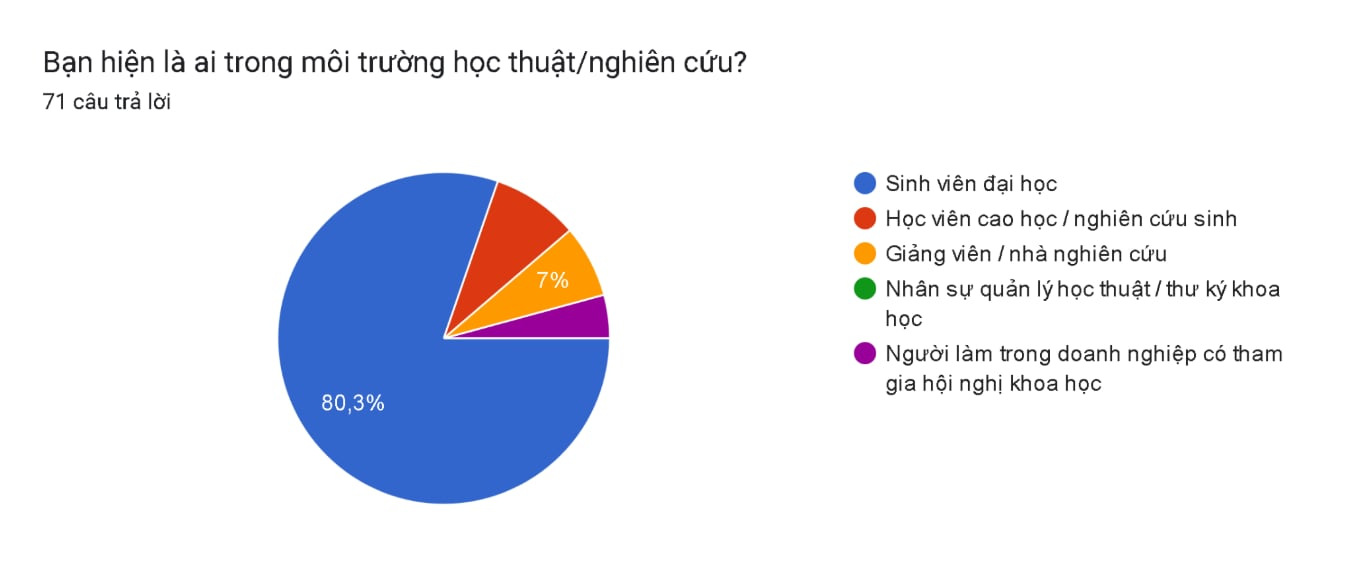
\includegraphics[width=0.9\textwidth]{images/chapter_2_picture_1.jpg}
    \caption{Phân bố đối tượng tham gia khảo sát}
    \label{fig:ch2-survey-participants}
\end{figure}

Hình~\ref{fig:ch2-survey-participants} trình bày phân bố mẫu khảo sát theo vai trò hoặc nhóm nghề nghiệp. Thành phần mẫu là cơ sở để xác định phạm vi diễn giải kết quả.

Trong phạm vi đề tài, ba nhóm vai trò được quan tâm nhất là:

\begin{itemize}
    \item \textbf{Tác giả:} người nộp bài, cần quy trình nộp bài dễ hiểu, giảm nhập liệu lặp lại, kiểm tra lỗi sớm và theo dõi trạng thái rõ ràng.
    \item \textbf{Phản biện viên:} người đọc và đánh giá bài báo, cần truy cập bài được phân công, nhanh chóng nắm được bối cảnh bài viết, viết nhận xét có chất lượng và giữ quyền tự quyết chuyên môn.
    \item \textbf{Chủ tọa/Đồng chủ tọa:} người có thẩm quyền cấu hình hội nghị, điều phối bài nộp, phân công phản biện viên, kiểm soát xung đột lợi ích và tổng hợp bằng chứng trước khi ra quyết định.
\end{itemize}

Cần lưu ý rằng số lượng phản hồi theo từng vai trò không đồng đều. Một số phân tích theo nhóm nhỏ như Chủ tọa hoặc Phản biện viên chỉ nên được đọc như tín hiệu định hướng, không phải kết luận thống kê đại diện cho toàn bộ cộng đồng học thuật.

\subsection{Phương pháp khảo sát}

Nhóm thực hiện khảo sát bằng biểu mẫu trực tuyến. Bộ câu hỏi gồm câu hỏi chọn một phương án, chọn nhiều phương án, câu hỏi theo thang Likert từ 1 đến 5 và câu hỏi mở. Cách thiết kế này vừa giúp lượng hóa mức độ phổ biến của các vấn đề, vừa thu thập lý do người dùng tin tưởng hoặc chưa tin tưởng các tính năng AI.

Các nhóm câu hỏi chính gồm:

\begin{itemize}
    \item Trải nghiệm với các nền tảng hiện có như EasyChair, Microsoft CMT và OpenReview.
    \item Các khó khăn thường gặp trong quy trình nộp bài, phản biện và quản lý hội nghị.
    \item Mức độ hữu ích của các tính năng dự kiến cho từng vai trò.
    \item Mức độ chấp nhận AI trong các tác vụ như tự động điền thông tin, kiểm tra sơ bộ bài nộp, hỗ trợ đọc bài, rà soát chất lượng phản biện và tổng hợp thông tin cho Chủ tọa.
\end{itemize}

Do khảo sát sử dụng mẫu thuận tiện, nhóm chỉ dùng kết quả để định hướng thiết kế và ưu tiên tính năng, không dùng để khẳng định xu hướng chung của toàn bộ cộng đồng nghiên cứu. Vì vậy, Chương 2 kết hợp dữ liệu khảo sát nội bộ với nguồn bên ngoài về áp lực xét duyệt học thuật và các hệ thống quản lý hội nghị hiện có.

\subsection{Kết quả khảo sát theo các vấn đề nổi bật}

Kết quả khảo sát cho thấy các khó khăn tập trung vào năm nhóm: thiếu chỉ dẫn về bước tiếp theo, biểu mẫu nhập liệu dài, phải đọc nhiều hướng dẫn dài, thiếu kiểm tra lỗi sớm, cùng tình trạng thông báo và hạn chót bị phân tán.

\begin{figure}[htbp]
    \centering
    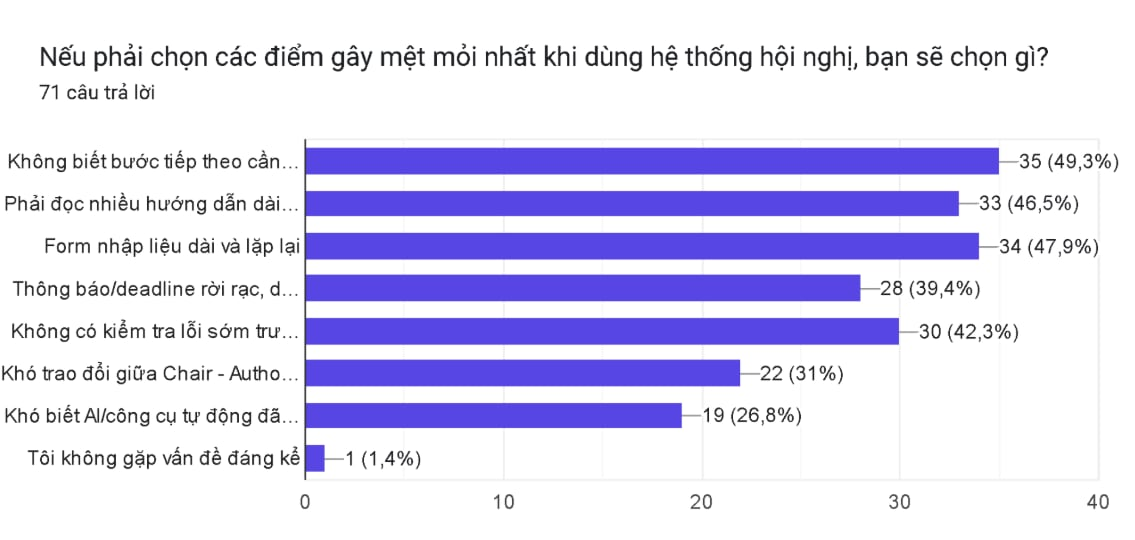
\includegraphics[width=0.9\textwidth]{images/chapter_2_picture_2.jpg}
    \caption{Các vấn đề người dùng gặp phải khi tham gia quy trình hội nghị khoa học}
    \label{fig:ch2-user-pain-points}
\end{figure}

Hình~\ref{fig:ch2-user-pain-points} minh họa phân bố các vấn đề nổi bật. Bảng dưới đây trình bày số liệu thu được từ khảo sát của nhóm.

\begin{center}
\small
\begin{tabular}{|P{0.23\textwidth}|P{0.23\textwidth}|P{0.23\textwidth}|P{0.23\textwidth}|}
\hline
Vấn đề nổi bật & Số người chọn & Tỷ lệ trên 71 phản hồi & Diễn giải thiết kế \\ \hline
Không biết bước tiếp theo cần làm là gì & 35 & 49,3\% & Hệ thống cần bảng điều khiển và lời nhắc hành động theo trạng thái, tránh để người dùng tự dò quy trình. \\ \hline
Biểu mẫu nhập liệu dài và lặp lại & 34 & 47,9\% & Quy trình nộp bài cần hỗ trợ trích xuất siêu dữ liệu từ tệp bài báo và cho phép người dùng chỉnh sửa trước khi gửi. \\ \hline
Phải đọc nhiều hướng dẫn dài trước khi thao tác & 33 & 46,5\% & Giao diện cần tổ chức thao tác theo từng bước, sử dụng ngôn ngữ rõ ràng và cung cấp trợ lý theo ngữ cảnh. \\ \hline
Không có kiểm tra lỗi sớm trước khi nộp chính thức & 30 & 42,3\% & Hệ thống cần kiểm tra sơ bộ trước khi bài nộp đi vào quy trình phản biện chính thức. \\ \hline
Thông báo và hạn chót bị phân tán, dễ bỏ sót & 28 & 39,4\% & Hệ thống cần tập trung thông báo và cập nhật trạng thái, thay vì phụ thuộc hoàn toàn vào thư điện tử. \\ \hline
\end{tabular}
\end{center}

Những số liệu này cho thấy khó khăn của người dùng không chỉ bắt nguồn từ việc thiếu chức năng nghiệp vụ. Nhiều hệ thống hiện có đã hỗ trợ nộp bài, phản biện và ra quyết định, nhưng quy trình thao tác vẫn phức tạp, phân tán và khó theo dõi. Vì vậy, ConferenceSpace không chỉ cần bao phủ các nghiệp vụ quản lý hội nghị mà còn phải giảm số bước và lượng thông tin người dùng phải nhập hoặc kiểm tra nhiều lần.

\subsection{Kết quả theo vai trò}

\subsubsection{a) Nhóm Chủ tọa/Ban tổ chức}

Trong nhóm người tham gia với vai trò Chủ tọa, các tính năng được quan tâm gồm cảnh báo xung đột lợi ích, bảng điều khiển trạng thái hội nghị và hỗ trợ phân công Phản biện viên. Tuy nhiên, số lượng Chủ tọa trong mẫu còn nhỏ nên các tỷ lệ của nhóm này chỉ có giá trị định hướng ưu tiên ban đầu.

\begin{center}
\small
\begin{tabular}{|P{0.31\textwidth}|P{0.31\textwidth}|P{0.31\textwidth}|}
\hline
Tính năng & Kết quả ghi nhận & Diễn giải \\ \hline
Cảnh báo xung đột lợi ích & 5/7 Chủ tọa đánh giá cao & Chủ tọa cần cơ chế cảnh báo sớm để tránh phân công sai người, nhưng kết quả cuối cùng vẫn cần người có thẩm quyền xác nhận. \\ \hline
Bảng điều khiển tóm tắt tình trạng hội nghị & 4/7 Chủ tọa đánh giá cao & Nhu cầu chính là giảm tải việc theo dõi thủ công qua nhiều bảng, thư điện tử và trang trạng thái rời rạc. \\ \hline
Gợi ý Phản biện viên theo chuyên môn & 2/7 Chủ tọa đánh giá cao & Tín hiệu này cho thấy Chủ tọa có thể thận trọng với việc tự động hóa phân công Phản biện viên; vì vậy, hệ thống nên trình bày gợi ý dưới dạng danh sách có điểm số và lý do rõ ràng, thay vì đưa ra quyết định tự động. \\ \hline
\end{tabular}
\end{center}

Tính năng đối sánh phản biện trong ConferenceSpace thuộc lớp thuật toán xác định, không phải luồng AI tạo sinh. Chủ tọa cần biết căn cứ xếp hạng phản biện viên, xung đột lợi ích nào đang ngăn việc phân công và có quyền ghi đè kết quả khi có căn cứ nghiệp vụ.

\subsubsection{b) Nhóm Tác giả}

Đối với Tác giả, nhu cầu nổi bật nhất là giảm lượng thông tin phải nhập trong quy trình nộp bài. Có 21 người chọn phương án ``tự điền và cho phép tôi sửa nhanh những mục sai'' cho chức năng Submission Autofill. Kết quả này cho thấy người dùng muốn hệ thống thực hiện các thao tác lặp lại nhưng không tự gửi bài thay họ; bước xác nhận vẫn thuộc trách nhiệm của Tác giả.

\begin{center}
\small
\begin{tabular}{|P{0.31\textwidth}|P{0.31\textwidth}|P{0.31\textwidth}|}
\hline
Tính năng & Kết quả ghi nhận & Diễn giải \\ \hline
Submission Autofill & Lựa chọn phổ biến nhất là tự điền nhưng cho phép sửa & Tính năng này nên tạo dữ liệu nháp, hiển thị các trường đã trích xuất và cho phép Tác giả chỉnh sửa. \\ \hline
Submission Gating & Người tham gia đánh giá tính năng này là hữu ích & Submission Gating nên cảnh báo lỗi sớm, nhưng không được tự động loại bài khi chưa có chính sách rõ ràng. \\ \hline
\end{tabular}
\end{center}

Xét về thiết kế, đây là nhóm tính năng ảnh hưởng trực tiếp nhất đến trải nghiệm ban đầu của Tác giả với hệ thống. Quy trình nộp bài cần giúp người dùng hoàn thành đúng yêu cầu, hiểu rõ trạng thái và sửa lỗi trước hạn chót.

\subsubsection{c) Nhóm Phản biện viên}

\begin{figure}[htbp]
    \centering
    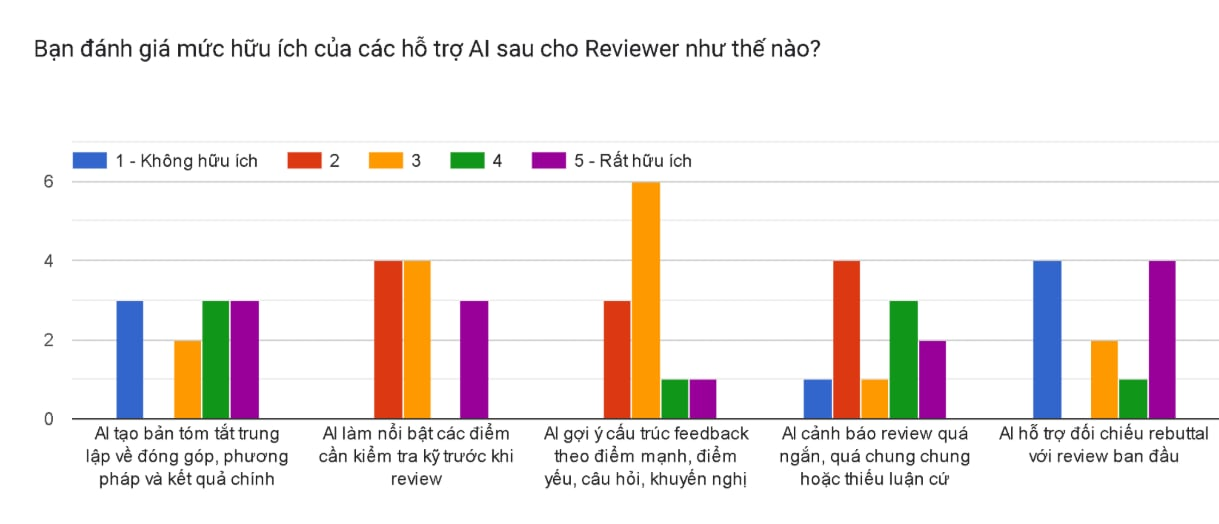
\includegraphics[width=0.9\textwidth]{images/chapter_2_picture_3.jpg}
    \caption{Mức độ ủng hộ AI của Phản biện viên theo từng tác vụ}
    \label{fig:ch2-reviewer-ai-acceptance}
\end{figure}

Hình~\ref{fig:ch2-reviewer-ai-acceptance} thể hiện mức độ chấp nhận AI của Phản biện viên theo từng tác vụ. Trong dữ liệu khảo sát, 6/11 Phản biện viên đánh giá cao tính năng dùng AI để tạo bản tóm tắt trung lập, trong khi chỉ 3/11 đánh giá cao tính năng dùng AI để nêu bật những điểm cần kiểm tra kỹ.

\begin{center}
\small
\begin{tabular}{|P{0.31\textwidth}|P{0.31\textwidth}|P{0.31\textwidth}|}
\hline
Tính năng & Kết quả ghi nhận & Diễn giải \\ \hline
Tóm tắt trung lập bài báo & 6/11 Phản biện viên đánh giá cao & AI có thể giúp Phản biện viên nắm bối cảnh ban đầu, nhưng bản tóm tắt không thay thế việc đọc bài. \\ \hline
Nêu bật điểm cần kiểm tra kỹ & 3/11 Phản biện viên đánh giá cao & Phản biện viên thận trọng với việc AI định hướng đánh giá học thuật; đầu ra nên là gợi ý kiểm tra, không phải kết luận chuyên môn. \\ \hline
\end{tabular}
\end{center}

Kết quả này phù hợp với các chính sách gần đây của những hội nghị lớn: AI có thể hỗ trợ Phản biện viên trong điều kiện được kiểm soát, nhưng Phản biện viên vẫn chịu trách nhiệm cuối cùng về nội dung bản phản biện, tính bảo mật của bản thảo và tính trung thực của đánh giá \cite{ch2ref15,ch2ref16}.

Do đó, AI chỉ nên hỗ trợ Phản biện viên định hướng việc đọc, không thay con người đọc và đánh giá bài báo. Khảo sát chưa đo khối lượng ghi chú, số lần đối chiếu hoặc thời gian rà soát; kết quả chỉ cho thấy người tham gia có xu hướng chấp nhận AI ở vai trò tạo bản tóm tắt và nêu những điểm cần kiểm tra.

\subsection{Diễn giải kết quả và giới hạn khảo sát}

Tổng hợp các phản hồi cho thấy bốn nhu cầu nền tảng:

\begin{enumerate}
    \item \textbf{Giảm thao tác thủ công:} người dùng muốn hệ thống xử lý phần nhập liệu và kiểm tra lặp lại, đặc biệt ở bước nộp bài.
    \item \textbf{Giảm tải nhận thức:} người dùng cần biết trạng thái hiện tại, việc tiếp theo cần làm và hạn chót liên quan mà không phải tự dò nhiều trang hoặc thư điện tử.
    \item \textbf{Tăng khả năng kiểm soát rủi ro:} Chủ tọa cần công cụ hỗ trợ phát hiện xung đột lợi ích và theo dõi tiến độ phản biện; Tác giả cần phát hiện lỗi trước khi gửi chính thức.
    \item \textbf{Bảo đảm tính minh bạch của AI:} người dùng chấp nhận AI khi công nghệ này chỉ đóng vai trò hỗ trợ, đưa ra kết quả có căn cứ và cho phép con người kiểm tra lại.
\end{enumerate}

Những kết luận này cần được diễn giải trong ba giới hạn. Thứ nhất, khảo sát sử dụng mẫu thuận tiện gồm 71 phản hồi nên không thể đại diện cho toàn bộ cộng đồng học thuật. Thứ hai, nhóm Chủ tọa và nhóm Phản biện viên có quy mô nhỏ; do đó, phân tích theo vai trò chỉ mang tính định hướng. Thứ ba, khảo sát này đo nhu cầu trước khi người tham gia sử dụng hệ thống, khác với khảo sát sau trải nghiệm được trình bày trong chương đánh giá.

\section{Khảo sát hiện trạng các hệ thống quản lý hội nghị}

\subsection{Đối tượng, tiêu chí và giới hạn khảo sát}

Nhóm chia các hệ thống khảo sát thành hai nhóm với mục đích đối chiếu khác nhau. Nhóm thứ nhất gồm EasyChair, HotCRP, OpenReview và Microsoft CMT. Các nền tảng này đã hoàn thiện quy trình nghiệp vụ và cung cấp chuẩn tham chiếu về vòng đời xét duyệt, vai trò, phân quyền, phân công, xung đột lợi ích, phản biện, phản hồi của tác giả và ra quyết định. Nhóm thứ hai gồm PeerSubmit, nền tảng lấy AI làm trọng tâm, và Morressier, đối tượng tham khảo bổ sung. PeerSubmit minh họa chiến lược đưa AI vào nhiều công đoạn của vòng đời; Morressier bổ sung góc nhìn về sàng lọc liêm chính, khai báo xung đột lợi ích và phân công phản biện có sự xác nhận của ban tổ chức.

Nhóm đối chiếu các nền tảng theo tám tiêu chí:

\begin{itemize}
    \item Mức bao phủ vòng đời xét duyệt và các vai trò được hỗ trợ;
    \item Các khâu tích hợp AI hoặc thuật toán trong vòng đời;
    \item Loại đầu ra được tạo và mức độ gần với quyết định học thuật;
    \item Cơ chế xác nhận, ghi đè hoặc chặn hành động;
    \item Khả năng giải thích, truy vết và kiểm tra lại kết quả;
    \item Phạm vi phân quyền đối với dữ liệu bài nộp và dữ liệu người dùng;
    \item Loại bằng chứng hỗ trợ cho từng nhận định;
    \item Các chức năng ngoài xét duyệt như đăng ký, thanh toán và trang thông tin sự kiện; tiêu chí này chỉ dùng để xác định phạm vi sản phẩm, không dùng để kết luận về chất lượng học thuật.
\end{itemize}

\subsection{Tổng quan các hệ thống hiện có}

\subsubsection{a) EasyChair}

EasyChair là hệ thống quản lý hội nghị có phạm vi sử dụng lớn theo số liệu do nhà cung cấp công bố. Trang chính thức của EasyChair nêu hơn 4,8 triệu người dùng và hơn 124.000 hội nghị đã sử dụng nền tảng này \cite{ch2ref1}. Hệ thống hỗ trợ nhiều thành phần của vòng đời hội nghị, bao gồm nộp bài, quản lý phản biện, quản lý quyền truy cập, xung đột lợi ích, phân công phản biện theo nguyện vọng, phản hồi của tác giả, thư điện tử, phân tích dữ liệu và xuất bản kỷ yếu \cite{ch2ref2}.

Bằng chứng từ cộng đồng hội nghị xác nhận EasyChair có thể vận hành một quy trình phản biện nhiều giai đoạn. ITiCSE 2025 sử dụng EasyChair cho phản biện kín hai chiều, đăng ký nguyện vọng phản biện, khai báo xung đột lợi ích, phân công bằng thuật toán, thảo luận và tổng hợp nhận xét của phản biện viên cấp cao \cite{ch2ref57}. Ở chiều ngược lại, một báo cáo kinh nghiệm công bố năm 2013 của thành viên ban tổ chức hội nghị ghi nhận rằng một số tùy chọn cấu hình khi đó khó tìm và phải thử nhiều lần mới hiểu, dù quy trình trở nên hữu ích sau khi người dùng đã làm quen \cite{ch2ref22}. Đây là một trường hợp sử dụng cụ thể, không đủ để kết luận EasyChair nhìn chung dễ hay khó sử dụng. Vì vậy, bài học phù hợp cho ConferenceSpace là tham khảo phạm vi quy trình của EasyChair, đồng thời đánh giá khả năng hướng dẫn theo ngữ cảnh bằng thử nghiệm người dùng của chính hệ thống thay vì suy diễn từ tài liệu hướng dẫn của EasyChair.

\subsubsection{b) HotCRP}

HotCRP hỗ trợ nhiều thành phần của quy trình phản biện và hoạt động điều phối của Chủ tọa. Theo tài liệu của HotCRP, hệ thống hỗ trợ phân công bài, đăng ký nguyện vọng phản biện, xung đột lợi ích, Chủ tọa ra quyết định, vai trò người điều phối thảo luận (lead), người hướng dẫn hoàn thiện bản sửa (shepherd), phân công tự động và chế độ chạy thử để kiểm tra kết quả trước khi áp dụng \cite{ch2ref3}. Tài liệu hướng dẫn dành cho Chủ tọa cũng mô tả cơ chế xử lý xung đột của Chủ tọa, quản trị viên phụ trách từng bài và có sử dụng cơ chế mã cấp quyền phản biện dùng để giới hạn quyền truy cập khi có xung đột \cite{ch2ref4}.

Báo cáo của hai đồng Chủ tọa chương trình USENIX ATC 2020 cung cấp bằng chứng vận hành cụ thể hơn. HotCRP hỗ trợ phân công hàng trăm bài cho hơn 100 thành viên ban chương trình; kết quả phân công tự động ban đầu được đánh giá là hữu ích nhưng vẫn cần Chủ tọa rà soát và điều chỉnh đáng kể. Báo cáo cũng ghi nhận danh mục chủ đề quá chi tiết làm tăng gánh nặng khai báo và có thể làm giảm chất lượng phân công ban đầu, trong khi cơ chế xung đột lợi ích ngăn thành viên có xung đột truy cập bài, điểm số và thảo luận liên quan \cite{ch2ref58}. Bằng chứng này xác nhận HotCRP đã được dùng để thực thi quy tắc truy cập và hỗ trợ Chủ tọa giám sát phân công, nhưng không chứng minh nền tảng chỉ phù hợp với người dùng có kinh nghiệm. ConferenceSpace vì vậy tham khảo nguyên tắc kiểm soát quyền và xác nhận phân công, còn mức độ dễ tiếp cận phải được đánh giá riêng trên người dùng của hệ thống.

\subsubsection{c) OpenReview}

OpenReview là nền tảng quản lý phản biện có khả năng cấu hình nhiều mức độ công khai. Trang giới thiệu chính thức mô tả đây là nền tảng đám mây cung cấp giao diện lập trình để truy cập dữ liệu theo quyền đọc và quyền ghi, hỗ trợ thảo luận mở, quản lý thông tin phục vụ xác định xung đột lợi ích và đối sánh bài báo với phản biện viên cho các hội nghị có hàng nghìn bài nộp \cite{ch2ref5}.

Các Chủ tọa chương trình NeurIPS 2021 đã chuyển toàn bộ quy trình sang OpenReview nhưng vẫn áp dụng phản biện kín hai chiều: trong thời gian xét duyệt, bài nộp chỉ hiển thị cho thành viên ban chương trình được phân công và các thảo luận nội bộ tiếp tục được giữ kín; chỉ bài được chấp nhận cùng các bản phản biện ẩn danh mới được công khai sau thời điểm thông báo \cite{ch2ref59}. Báo cáo sau hội nghị của các Chủ tọa chương trình ACT 2023 cũng cho thấy OpenReview phiên bản 1 có thể thích nghi với quy trình phản biện kín một chiều, nhưng một số xung đột lợi ích đặc thù, quyền xem thảo luận và việc thêm phản biện viên phụ vẫn cần cấu hình qua giao diện lập trình hoặc xử lý thủ công \cite{ch2ref60}. Vì vậy, điểm tham khảo có bằng chứng của OpenReview là khả năng cấu hình mức độ công khai và quyền truy cập; ConferenceSpace cần bảo đảm tính minh bạch có kiểm soát thay vì mặc định công khai toàn bộ quy trình.

\subsubsection{d) Microsoft CMT}

Microsoft CMT hỗ trợ nhiều vai trò, nhiều tiểu ban chuyên môn, toàn bộ vòng đời nộp bài, biểu mẫu tùy chỉnh, quản lý xung đột, đăng ký nguyện vọng phản biện, gợi ý phản biện viên, thảo luận, phản hồi của tác giả và phân công tích hợp với TPMS \cite{ch2ref6}. Tài liệu CMT về quản lý xung đột nêu hai cơ chế chính: xung đột theo cá nhân và xung đột theo miền thư điện tử; các xung đột này được xét trong quá trình phân công \cite{ch2ref7}. Theo tài liệu TPMS, điểm TPMS nằm trong khoảng từ 0 đến 1; điểm càng cao thì mức độ phù hợp giữa bài báo và phản biện viên càng lớn \cite{ch2ref8}.

Báo cáo của các Chủ tọa CVPR 2013 cho biết CMT đã quản lý toàn bộ quá trình nộp và xét duyệt 1.798 bài được phản biện đầy đủ. TPMS cung cấp gợi ý đối sánh; CMT chọn ba phản biện viên không có xung đột cho mỗi bài từ danh sách ứng viên; sau đó các Chủ tọa và Chủ tọa lĩnh vực vẫn thực hiện nhiều điều chỉnh thủ công để cải thiện mức độ phù hợp dưới ràng buộc về khối lượng công việc. Báo cáo kết luận trách nhiệm phân công thuộc về các Chủ tọa, còn CMT và TPMS đóng vai trò hỗ trợ \cite{ch2ref61}. Bằng chứng vận hành này củng cố cách ConferenceSpace thiết kế đối sánh như một chức năng hỗ trợ có thể kiểm tra, kết hợp điểm phù hợp chuyên môn, xung đột lợi ích, khối lượng công việc và quyền xác nhận của Chủ tọa, thay vì tự động ra quyết định cuối cùng.

\subsubsection{e) PeerSubmit: nền tảng lấy AI làm trọng tâm}

PeerSubmit tự định vị là nền tảng lấy AI làm trọng tâm trong quản lý bài nộp và xét duyệt. Tài liệu sản phẩm công bố một vòng đời chung gồm cấu hình hội nghị hoặc tạp chí, tiếp nhận bài, phân công phản biện viên, phản biện và ra quyết định. Nền tảng hỗ trợ nhiều tiểu ban chuyên môn, các chế độ phản biện kín một chiều, kín hai chiều và công khai, biểu mẫu chấm điểm, phản hồi của tác giả, nhiều vòng chỉnh sửa, phân quyền theo vai trò và nhật ký hoạt động \cite{ch2ref48}.

Danh mục chức năng AI trên trang sản phẩm gồm đối sánh phản biện theo chuyên môn kèm điểm tin cậy và kiểm tra xung đột lợi ích, tóm tắt bài nộp, sàng lọc chất lượng và mức độ phù hợp với phạm vi hội nghị, cùng bản tóm lược hỗ trợ quyết định (decision brief) tổng hợp điểm và nhận xét \cite{ch2ref48}. Bài viết kỹ thuật của nhà cung cấp mô tả phương pháp đối sánh bằng biểu diễn nhúng cho bài báo và hồ sơ phản biện viên, chỉ mục HNSW, truy vấn $K$ kết quả gần nhất, xếp hạng theo độ tương đồng cosine, sau đó lọc theo xung đột lợi ích và tình trạng sẵn sàng \cite{ch2ref53}. Đây là kiến trúc do nhà cung cấp mô tả; nguồn không công bố mô hình nhúng, dữ liệu đánh giá hoặc kết quả kiểm chứng độc lập, nên báo cáo không kết luận về việc triển khai thực tế hoặc chất lượng đối sánh.

Ranh giới trách nhiệm trong tài liệu PeerSubmit chưa hoàn toàn nhất quán. Trang sản phẩm mô tả Chủ tọa sử dụng bảng điều khiển quyết định để chấp nhận, từ chối hoặc yêu cầu sửa bài, còn bản tóm lược hỗ trợ quyết định chỉ tổng hợp điểm phản biện \cite{ch2ref48}. Bài viết về AI trong xét duyệt cũng khẳng định AI không đưa ra quyết định chấp nhận hoặc từ chối và phán đoán của con người vẫn giữ vai trò trung tâm \cite{ch2ref54}. Tuy nhiên, trang thông tin đồng thời quảng bá chức năng AI hỗ trợ chấm điểm bản phản biện và chức năng tạo phán quyết cuối cùng kèm điểm tin cậy \cite{ch2ref52}. Báo cáo xem sự khác biệt này là một giới hạn của tài liệu do nhà cung cấp công bố; nhóm không suy diễn rằng PeerSubmit hoàn toàn tự động ra quyết định, đồng thời không xem quyền ghi đè của con người là đặc điểm riêng của ConferenceSpace.

PeerSubmit tự công bố mức giảm 70\% đối với chu kỳ xét duyệt, 99\% đối với thời gian phân công và 40\% đối với thời gian phản biện, cùng tỷ lệ phù hợp giữa bài báo và phản biện viên là 96\% \cite{ch2ref48}. Trong phạm vi khảo sát, nhóm chưa tìm thấy báo cáo vận hành của một hội nghị, đánh giá cộng đồng hoặc nghiên cứu độc lập công bố dữ liệu nguồn, cỡ mẫu, tập tham chiếu, định nghĩa chỉ số và phương pháp đo tương ứng. Vì vậy, báo cáo chỉ xem các tỷ lệ này là tuyên bố của nhà cung cấp, không dùng làm kết quả thực nghiệm hoặc đường cơ sở cho ConferenceSpace. Tài liệu PeerSubmit cho thấy tự động hóa tại nhiều công đoạn là một chiến lược định vị sản phẩm. Do đó, câu hỏi có ý nghĩa đối với ConferenceSpace không còn là ``có tích hợp AI hay không'', mà là ``tác vụ nào nên dùng AI, tác vụ nào phải cho kết quả có thể tái tạo, ai xác nhận đầu ra và cần bằng chứng nào để đánh giá từng lựa chọn''.

\subsubsection{f) Morressier: tham khảo về liêm chính và phân công có xác nhận}

Morressier thể hiện một chiến lược khác: tích hợp kiểm tra đạo văn, trùng lặp hình ảnh và dấu hiệu của "cơ sở sản xuất bài báo hàng loạt" (paper mill) vào quy trình Integrity Manager để nhóm biên tập xem báo cáo trước khi ra quyết định \cite{ch2ref47}. Tài liệu Auto-Assign mô tả việc phân phối bài đều nhất có thể giữa các phản biện viên đã chấp nhận và tạo danh sách gợi ý để người tổ chức sửa trước khi xác nhận. Các điều kiện chặn được nêu cụ thể gồm phản biện viên đã được phân công cho bài, đã từ chối bài, là đồng tác giả của bài hoặc đã quá hạn phản biện \cite{ch2ref55}; phạm vi này không đủ để kết luận chức năng tự động phát hiện mọi dạng xung đột lợi ích. Từ phía cộng đồng xuất bản, IOP Publishing xác nhận đã hợp tác với Morressier để tích hợp luồng tiếp nhận, phản biện và xuất bản kỷ yếu cho các đơn vị tổ chức hội nghị mà IOP phục vụ \cite{ch2ref62}. Tuy nhiên, thông báo này được công bố năm 2021, trước khi Integrity Manager ra mắt, và không đánh giá Auto-Assign. Do đó, báo cáo chỉ dùng Morressier để tham khảo hai mẫu thiết kế cần được kiểm chứng thêm là sàng lọc liêm chính chuyên biệt và phân công có bước xác nhận, chứ không dùng làm bằng chứng về chất lượng hoặc hiệu quả của hai chức năng.

\subsection{So sánh phạm vi nghiệp vụ}

Bảng dưới đây xem xét liệu ConferenceSpace có đặt các thử nghiệm thuật toán và AI trong một vòng đời xét duyệt thống nhất hay chỉ ghép các luồng xử lý rời rạc. Mức hỗ trợ của các nền tảng đối chiếu được tổng hợp từ tài liệu công khai; cột ConferenceSpace chỉ mô tả phạm vi đề tài, không đánh giá chất lượng.

\begingroup
\small
\setlength{\tabcolsep}{2pt}
\setlength{\LTleft}{0pt}
\setlength{\LTright}{0pt}
\begin{longtable}{|P{0.17\textwidth}|P{0.20\textwidth}|P{0.20\textwidth}|P{0.20\textwidth}|P{0.17\textwidth}|}
  \caption{So sánh phạm vi nghiệp vụ của các nhóm nền tảng}\\
\hline
Nhóm nghiệp vụ & EasyChair/HotCRP & OpenReview/CMT & PeerSubmit & ConferenceSpace \\ \hline
\endfirsthead
\hline
Nhóm nghiệp vụ & EasyChair/HotCRP & OpenReview/CMT & PeerSubmit & ConferenceSpace \\ \hline
\endhead
\hline
\endfoot
Cấu hình hội nghị và chuyên đề & Có, với mức cấu hình khác nhau & Có & Có & Có trong phạm vi đề tài \\ \hline
Nộp bài, sửa bài và theo dõi trạng thái & Có & Có & Có & Có \\ \hline
Vai trò và phân quyền & Có & Có & Có, công bố cơ chế phân quyền theo vai trò & Có theo các vai trò Tác giả, Phản biện viên và Chủ tọa/Đồng chủ tọa \\ \hline
Phân công phản biện và xung đột lợi ích & Có cơ chế đăng ký nguyện vọng, ràng buộc hoặc khai báo xung đột & Có đối sánh, đăng ký nguyện vọng, TPMS và kiểm tra xung đột lợi ích & Có đối sánh kèm điểm tin cậy và kiểm tra xung đột lợi ích theo công bố của nhà cung cấp & Có thuật toán đối sánh xác định, cung cấp điểm và thông tin xung đột lợi ích để Chủ tọa xác nhận \\ \hline
Biểu mẫu, bản nháp và gửi bản phản biện & Có & Có & Có & Có \\ \hline
Phản hồi của tác giả, thảo luận và vòng chỉnh sửa & Có tùy cấu hình & Có & Có theo tài liệu sản phẩm & Có trong phạm vi luồng đã xây dựng \\ \hline
Quyết định và thông báo & Có & Có & Có bảng điều khiển quyết định và thư thông báo & Chủ tọa ra quyết định; hệ thống quản lý trạng thái và thông báo \\ \hline
Bản hoàn thiện sau chấp nhận & Có ở một số nền tảng & Có tùy quy trình & Có bước chấp nhận cuối cùng và công bố theo mô tả sản phẩm & Chỉ hỗ trợ tải lên và truy xuất tệp sau khi bài được chấp nhận; chưa có bước phê duyệt, thực thi hạn chót hoặc yêu cầu nộp lại \\ \hline
Đăng ký, thanh toán và trang thông tin sự kiện & Có ở một số gói hoặc qua tích hợp & Không phải trọng tâm chung & Có các chức năng sự kiện theo trang thông tin giá & Nằm ngoài phạm vi đề tài \\ \hline
\end{longtable}
\endgroup

Kết quả so sánh cho thấy ConferenceSpace tổ chức các thành phần nộp bài, phân công, xung đột lợi ích, phản biện, phản hồi của tác giả, ra quyết định và tải bản hoàn thiện sau chấp nhận trong cùng một mô hình trạng thái và quyền hạn. Vì vậy, các luồng hỗ trợ không phải những bản minh họa độc lập. Bảng chỉ xác nhận phạm vi đã xây dựng theo mô tả thiết kế, không xác nhận các chức năng vận hành đúng trong toàn bộ quy trình.

\subsection{So sánh với nền tảng có chiến lược lấy AI làm trọng tâm và quy ước trách nhiệm}

Bảng sau đối chiếu cách các nền tảng tích hợp cơ chế tự động hóa hoặc AI vào vòng đời xét duyệt. Mỗi ô mô tả quy ước được công bố về tác vụ, đầu ra và người xác nhận; bảng không nhằm xếp hạng chất lượng. Nội dung về PeerSubmit và Morressier dựa trên tuyên bố của nhà cung cấp, còn cột ConferenceSpace trình bày quy ước thiết kế. Mức độ triển khai và bằng chứng được đánh giá riêng ở Chương 4.

\begingroup
\small
\setlength{\tabcolsep}{2pt}
\setlength{\LTleft}{0pt}
\setlength{\LTright}{0pt}
\begin{longtable}{|P{0.16\textwidth}|P{0.24\textwidth}|P{0.27\textwidth}|P{0.27\textwidth}|}
  \caption{So sánh chiến lược AI và quy ước trách nhiệm}\\
\hline
Tác vụ & Nền tảng đã hoàn thiện nghiệp vụ/Morressier & PeerSubmit theo tài liệu nhà cung cấp & ConferenceSpace \\ \hline
\endfirsthead
\hline
Tác vụ & Nền tảng đã hoàn thiện nghiệp vụ/Morressier & PeerSubmit theo tài liệu nhà cung cấp & ConferenceSpace \\ \hline
\endhead
\hline
\endfoot
Nhập liệu và sàng lọc & Các nền tảng đã hoàn thiện nghiệp vụ sử dụng biểu mẫu; Morressier công bố chức năng kiểm tra trước khi nộp và kiểm tra liêm chính chuyên biệt & Công bố chức năng sàng lọc chất lượng và mức độ phù hợp với phạm vi hội nghị, trích xuất chủ đề và từ khóa & Submission Autofill tạo bản nháp để Tác giả sửa và xác nhận; Submission Gating tách lỗi theo quy tắc khỏi cảnh báo về nội dung do AI phát hiện \\ \hline
Đối sánh phản biện & CMT sử dụng TPMS; Morressier phân công tự động theo chủ đề, tải và xung đột, sau đó người tổ chức xác nhận & Sử dụng biểu diễn nhúng, HNSW, truy vấn $K$ kết quả gần nhất, độ tương đồng cosin và bộ lọc xung đột lợi ích; Chủ tọa có thể phê duyệt hoặc ghi đè gợi ý & Sử dụng Jaccard cùng ràng buộc về khối lượng công việc và xung đột lợi ích để cho kết quả xác định; Chủ tọa xác nhận hoặc ghi đè quyết định \\ \hline
Phát hiện xung đột lợi ích & Nhiều nền tảng có cơ chế khai báo hoặc quy tắc xung đột; Morressier chặn một số trường hợp phân công & Công bố chức năng tự động kiểm tra xung đột lợi ích trong quá trình đối sánh & Kết hợp tự kiểm tra, khai báo và đồ thị đồng tác giả; hiển thị bằng chứng nhưng không tuyên bố phát hiện đầy đủ \\ \hline
Tóm tắt bài nộp & Không phải năng lực cốt lõi chung của nhóm nền tảng đã hoàn thiện nghiệp vụ & Công bố chức năng tóm tắt phương pháp, đóng góp và cảnh báo các vấn đề về chất lượng & Reviewer Initial Analysis tạo bản tóm tắt, nêu điểm mạnh, điểm yếu, gợi ý; không tự điền, gửi, chấm điểm hoặc đưa ra khuyến nghị cuối cùng trong biểu mẫu phản biện \\ \hline
Rà soát bản phản biện & Sử dụng biểu mẫu và quy tắc nghiệp vụ; Morressier tập trung vào tính liêm chính của bài nộp & Trang thông tin giá công bố chức năng AI hỗ trợ chấm điểm bản phản biện và phát hiện nội dung không nhất quán & Review Quality Auditor rà soát bản phản biện nháp trước khi gửi để  \\ \hline
Tổng hợp thông tin trước quyết định & Cung cấp bảng điểm, thảo luận và chức năng ra quyết định của Chủ tọa tùy nền tảng & Công bố bản tóm lược hỗ trợ quyết định; trang thông tin giá còn quảng bá chức năng tạo phán quyết cuối cùng, trong khi bài viết khác vẫn giao quyền chấp nhận hoặc từ chối cho con người & Chair Decision Copilot tổng hợp bằng chứng và bất đồng; chức năng này không tạo phán quyết chấp nhận hoặc từ chối bài báo \\ \hline
Trợ lý cho nhiều vai trò & Chưa ghi nhận đây là năng lực cốt lõi chung & Chưa đủ tài liệu công khai để kết luận về quy ước truy cập tài nguyên theo từng vai trò & Chatbot Agent chỉ gọi công cụ trong phạm vi quyền và từ chối yêu cầu ngoài phạm vi, ngoài quyền truy cập \\ \hline
Loại bằng chứng & Tài liệu sản phẩm và hỗ trợ; một số cơ chế có nghiên cứu riêng & Chủ yếu là tài liệu và số liệu do nhà cung cấp công bố; nhóm chưa xác nhận được đánh giá độc lập & Mã nguồn, kết quả kiểm thử, đánh giá theo tác vụ và kiểm thử chấp nhận của người dùng ở Chương 4; mức độ bằng chứng khác nhau giữa các luồng \\ \hline
\end{longtable}
\endgroup


\subsection{Đối chiếu kết quả khảo sát với bằng chứng bên ngoài và chính sách học thuật}

Khảo sát nhu cầu sử dụng mẫu thuận tiện, trong đó số người tham gia với vai trò Chủ tọa và Phản biện viên còn nhỏ. Vì vậy, nhóm đối chiếu các nguyên tắc rút ra từ khảo sát với nguồn bên ngoài để kiểm tra tính phù hợp với thực tiễn vận hành và chính sách học thuật. Bước đối chiếu này không nhằm ước lượng tỷ lệ nhu cầu trong toàn bộ cộng đồng, xác lập khoảng trống thị trường hoặc chứng minh hiệu quả của ConferenceSpace.

Nhóm phân biệt bốn loại nguồn theo phạm vi có thể kết luận. Tài liệu sản phẩm chỉ xác nhận chức năng được công bố; báo cáo của Chủ tọa hoặc ban chương trình cung cấp bằng chứng về cách một hội nghị cụ thể đã vận hành; chính sách của hội nghị, hiệp hội và nhà xuất bản xác định trách nhiệm cùng giới hạn sử dụng AI; nghiên cứu có công bố phương pháp cung cấp bằng chứng thực nghiệm trong phạm vi mẫu và thiết kế nghiên cứu. Nhóm ưu tiên nguồn chính thức và nghiên cứu gốc, đồng thời giữ lại các trường hợp khác biệt giữa chính sách thay vì xem một quy định đơn lẻ là đồng thuận của toàn cộng đồng.

Đối với phân công phản biện, các báo cáo vận hành củng cố yêu cầu kết hợp thuật toán với quyền kiểm soát của con người. Tại USENIX ATC 2020, kết quả phân công ban đầu của HotCRP được các đồng Chủ tọa đánh giá là hữu ích nhưng vẫn cần rà soát và điều chỉnh đáng kể \cite{ch2ref58}. Tại CVPR 2013, TPMS cung cấp kết quả đối sánh, CMT chọn các Phản biện viên không có xung đột từ danh sách ứng viên, sau đó Chủ tọa và Chủ tọa lĩnh vực tiếp tục điều chỉnh dưới ràng buộc về khối lượng công việc \cite{ch2ref61}. Hai trường hợp không chứng minh một thuật toán cụ thể tốt hơn các phương pháp khác, nhưng xác nhận rằng điểm phù hợp, xung đột lợi ích, khối lượng công việc và bước xác nhận là các thành phần riêng biệt của quy trình phân công.

Yêu cầu phát hiện xung đột lợi ích qua nhiều nguồn cũng phù hợp với chính sách học thuật. ACM quy định người tham gia phải khai báo xung đột tiềm ẩn, nhưng đồng thời nhấn mạnh một chính sách đáng tin cậy không thể chỉ dựa vào việc mỗi cá nhân tự xác định xung đột của mình; người phụ trách như Chủ tọa hoặc biên tập viên vẫn phải đánh giá và xử lý trường hợp được báo cáo \cite{ch2ref12}. Do đó, kết quả từ quy tắc, đồ thị đồng tác giả hoặc dữ liệu học thuật bên ngoài trong ConferenceSpace chỉ nên được trình bày như bằng chứng hỗ trợ để Chủ tọa xem xét, không phải kết luận tự động rằng một cặp bài báo-Phản biện viên chắc chắn có hoặc không có xung đột.

Nhu cầu kiểm tra liêm chính có bằng chứng khảo sát bên ngoài, nhưng phạm vi trách nhiệm còn chưa thống nhất. Nghiên cứu của Calamur và Ghosh phân tích khảo sát năm 2022 với 852 người tham gia; sau khi loại 22 người không đồng ý tham gia và 145 người không trả lời câu hỏi nào, phân tích còn 685 phiếu có dữ liệu. Trong 401 người từng thực hiện phản biện, 174 người (43,39\%) cho biết đã gặp bản thảo bị nghi ngờ vi phạm liêm chính; 540 người trong mẫu phân tích (78,83\%) kỳ vọng quy trình phản biện có khả năng nhận diện đạo văn \cite{ch2ref56}. Các tác giả đồng thời đặt vấn đề liệu trách nhiệm này thuộc về Phản biện viên, nhóm biên tập hay công cụ chuyên biệt. Vì vậy, các tỷ lệ trên củng cố nhu cầu có bước sàng lọc và chuyển bằng chứng cho người có thẩm quyền, nhưng không chứng minh AI có thể tự xác định hành vi vi phạm.

Các chính sách AI được khảo sát hội tụ ở hai yêu cầu: bảo mật bản thảo và giữ trách nhiệm ở con người; tuy nhiên, phạm vi sử dụng được phép khác nhau đáng kể. ICLR 2026 cho phép dùng mô hình ngôn ngữ lớn để cải thiện ngữ pháp và độ rõ của bản phản biện nếu khai báo, nhưng Phản biện viên vẫn chịu trách nhiệm về nội dung và không được vi phạm tính bảo mật của bài chưa công bố \cite{ch2ref15}. Ngược lại, ICML 2025 cấm Phản biện viên dùng AI tạo sinh để viết bản phản biện hoặc đưa bất kỳ nội dung nào của bài nộp hay bản phản biện vào công cụ AI tạo sinh \cite{ch2ref16}. ACM cho phép dùng công cụ để cải thiện văn bản do Phản biện viên viết nếu trước đó đã loại toàn bộ thông tin có thể nhận diện bài nộp, Tác giả và Phản biện viên. ACM cũng cho phép dùng hệ thống có cam kết duy trì tính bảo mật của thông tin được tải lên; trong cả hai trường hợp, Phản biện viên vẫn chịu trách nhiệm về thiên lệch và nội dung được tạo \cite{ch2ref40}. Nature Portfolio yêu cầu Phản biện viên không tải bản thảo lên công cụ AI tạo sinh và phải khai báo nếu AI hỗ trợ bất kỳ phần nào của việc đánh giá các tuyên bố trong bài \cite{ch2ref41}. Sự khác biệt này cho thấy chức năng AI cho Phản biện viên phải có khả năng bật, tắt hoặc giới hạn theo chính sách của từng hội nghị; một cấu hình chung không thể mặc nhiên phù hợp với mọi nơi.

Bằng chứng thực nghiệm hiện có cũng ủng hộ cách tiếp cận thử nghiệm có kiểm soát thay vì giả định AI luôn cải thiện phản biện. Tại ICLR 2025, Review Feedback Agent chỉ cung cấp góp ý tùy chọn trên bản phản biện do con người đã viết và không trực tiếp sửa nội dung. Trong thử nghiệm ngẫu nhiên quy mô lớn, 26,6\% Phản biện viên nhận góp ý đã cập nhật bản phản biện; nhóm nghiên cứu còn báo cáo bản phản biện được sửa dài hơn và được đánh giá cao hơn trong phép đánh giá mù, nhưng thừa nhận cần tiếp tục nghiên cứu giới hạn của phản hồi do AI tạo \cite{ch2ref17,ch2ref18}. NeurIPS 2026 tiếp tục khảo sát một phạm vi rộng hơn bằng thử nghiệm tự nguyện: Tác giả và Phản biện viên phải đồng ý tham gia, các phân công được chia ngẫu nhiên giữa điều kiện không dùng AI và hai điều kiện hỗ trợ, dữ liệu không được nhà cung cấp lưu giữ, còn Chủ tọa lĩnh vực đánh giá bản phản biện mà không biết điều kiện thử nghiệm. Công cụ được định vị để hỗ trợ hiểu và phân tích bài, không viết bản phản biện hoặc thay thế phán đoán của Phản biện viên \cite{ch2ref19}. Vì thử nghiệm NeurIPS chưa công bố kết quả tại thời điểm khảo sát, báo cáo chỉ dùng thiết kế này làm tham chiếu về biện pháp kiểm soát, không dùng làm bằng chứng về hiệu quả.

Việc đối chiếu vì vậy củng cố ba yêu cầu cho ConferenceSpace: phân công và phát hiện xung đột lợi ích phải cung cấp căn cứ để Chủ tọa xác nhận; chức năng AI phải tuân theo chính sách bảo mật và trách nhiệm của từng hội nghị; hiệu quả của mỗi luồng AI phải được đo riêng trong điều kiện sử dụng xác định. Các nhu cầu về giảm nhập liệu, chỉ dẫn bước tiếp theo và thông báo tập trung vẫn chủ yếu bắt nguồn từ khảo sát nội bộ và không được khái quát bằng các nguồn bên ngoài nêu trên. Chương 4 đánh giá mức độ đáp ứng của ConferenceSpace trong phạm vi dữ liệu, phép thử và kiểm thử chấp nhận của người dùng đã thực hiện.

\section{Vấn đề thực tiễn và nguyên tắc giải pháp}

\subsection{Các vấn đề thiết kế rút ra từ khảo sát}

Các nền tảng đã hoàn thiện phần lớn nghiệp vụ cốt lõi, còn PeerSubmit và Morressier cho thấy AI hoặc cơ chế tự động hóa đã xuất hiện ở nhiều công đoạn. Vì vậy, vấn đề của đề tài không còn là thị trường ``thiếu AI tích hợp'', mà là cách xử lý các tác vụ khác nhau về mức độ nghiêm trọng của hậu quả, yêu cầu đối với tính ổn định và chủ thể chịu trách nhiệm. Từ đó, nhóm xác định năm vấn đề thiết kế.

\textbf{Thứ nhất, giảm nhập liệu không được loại bỏ bước xác nhận của Tác giả.} Gần một nửa số người tham gia khảo sát chọn biểu mẫu dài và lặp lại là vấn đề nổi bật. Submission Autofill có thể tạo siêu dữ liệu nháp, nhưng Tác giả phải có quyền sửa từng trường và quyết định thời điểm gửi bài.

\textbf{Thứ hai, đối sánh phản biện và phát hiện xung đột lợi ích cần cho kết quả ổn định, có căn cứ.} TPMS, PeerSubmit và Morressier cho thấy nhiều chiến lược đối sánh đã được triển khai \cite{ch2ref8,ch2ref53,ch2ref55}. Tuy nhiên, phân công sai có thể ảnh hưởng đến tính công bằng và bảo mật. Vì vậy, ConferenceSpace sử dụng thuật toán xác định, hiển thị điểm số, lý do và ràng buộc, sau đó để Chủ tọa xác nhận. Lựa chọn này không hàm ý Domain Jaccard tốt hơn phương pháp đối sánh theo ngữ nghĩa.

\textbf{Thứ ba, nội dung hỗ trợ đọc và tổng hợp phải bám sát bằng chứng, đồng thời đi kèm phân tích.} Tóm tắt, cảnh báo hoặc nội dung tổng hợp có thể giảm tải nhận thức, nhưng đầu ra không cố định có thể bỏ sót thông tin, suy diễn thiếu căn cứ hoặc gây nhiễu. Mỗi luồng cần được đánh giá bằng chỉ số riêng, có phân tích các trường hợp sai và chỉ được kết luận trong phạm vi dữ liệu đã đo.

\textbf{Thứ tư, các luồng xử lý gần bước ra quyết định phải công khai mức độ ảnh hưởng đến quyền tác giả của Phản biện viên và phán quyết học thuật.} Chính sách ICLR yêu cầu người tham gia chịu trách nhiệm về nội dung của mình; ICML cấm Phản biện viên dùng AI tạo sinh để viết bản phản biện hoặc đưa nội dung mật vào công cụ AI \cite{ch2ref15,ch2ref16}. Nghiên cứu Review Feedback Agent chỉ hỗ trợ góp ý trên bản nháp do con người viết \cite{ch2ref17,ch2ref18}. ConferenceSpace không cho phép AI tự điền hoặc gửi biểu mẫu, chấm điểm hay tạo phán quyết chấp nhận hoặc từ chối.

\textbf{Thứ năm, trợ lý phục vụ nhiều vai trò phải giữ đúng ranh giới truy cập tài nguyên.} Chatbot Agent chỉ được truy vấn dữ liệu mà người dùng hiện tại có quyền xem; hệ thống phải từ chối yêu cầu ngoài phạm vi thay vì trả lời bằng suy đoán. Cơ chế phân quyền ở cấp ứng dụng không có nghĩa là hệ thống đã kiểm toán toàn bộ vòng đời lưu giữ, sử dụng để huấn luyện hoặc vị trí lưu trữ dữ liệu của nhà cung cấp AI.

Mô hình ba lớp là lựa chọn thiết kế để xử lý năm vấn đề trên: lớp nghiệp vụ cốt lõi quản lý trạng thái và quyền hạn; lớp thuật toán xác định và có thể kiểm chứng xử lý đối sánh, xung đột lợi ích và các quy tắc; lớp AI hỗ trợ có kiểm soát tạo bản nháp, phân tích, cảnh báo hoặc tổng hợp. Báo cáo không xem mô hình này là điểm mới của thị trường hay kiến trúc tối ưu duy nhất.

\subsection{Liên kết vấn đề với định hướng giải pháp}

ConferenceSpace được thiết kế để xử lý năm vấn đề trên trong phạm vi một vòng đời xét duyệt chung. Bảng sau liên kết từng vấn đề với chức năng liên quan và ranh giới trách nhiệm; mối liên kết này giải thích lựa chọn thiết kế, không thay thế bằng chứng đánh giá ở Chương 4.

\begingroup
\small
\setlength{\tabcolsep}{2pt}
\setlength{\LTleft}{0pt}
\setlength{\LTright}{0pt}
\begin{longtable}{|P{0.31\textwidth}|P{0.31\textwidth}|P{0.31\textwidth}|}
  \caption{Liên kết vấn đề thiết kế với định hướng giải pháp ConferenceSpace}\\
\hline
Vấn đề thiết kế & Định hướng trong ConferenceSpace & Ranh giới trách nhiệm \\ \hline
\endfirsthead
\hline
Vấn đề thiết kế & Định hướng trong ConferenceSpace & Ranh giới trách nhiệm \\ \hline
\endhead
\hline
\endfoot
Nộp bài thủ công, biểu mẫu dài & Submission Autofill trích xuất siêu dữ liệu từ tệp PDF và gợi ý chuyên đề trong phạm vi hội nghị & Đầu ra là bản nháp có thể chỉnh sửa; Tác giả xác nhận trước khi gửi \\ \hline
Thiếu kiểm tra lỗi sớm & Submission Gating kiểm tra các điều kiện cơ bản trước khi bài nộp đi vào quy trình phản biện & Cảnh báo hoặc chặn theo chính sách đã cấu hình; không tự động loại bài ngoài các quy tắc của hệ thống \\ \hline
Khó kiểm soát việc đối sánh phản biện và xung đột lợi ích & Thuật toán đối sánh cung cấp điểm số và kết hợp nhiều lớp phát hiện xung đột lợi ích & Đối sánh phản biện thuộc lớp thuật toán xác định; Chủ tọa ra quyết định cuối cùng \\ \hline
Phản biện viên thiếu công cụ hỗ trợ đọc hiểu ban đầu và phải tự ghi chú nhiều điểm cần kiểm tra & Reviewer Initial Analysis cung cấp bản tóm tắt, các điểm cần kiểm tra và căn cứ liên quan & AI hỗ trợ định hướng đọc; khảo sát chưa đo mức giảm thao tác, thời gian rà soát hoặc ảnh hưởng đến đánh giá chuyên môn \\ \hline
Phản biện viên cần hỗ trợ rà soát bản nháp; Chủ tọa khó tổng hợp nhiều bản phản biện và phản hồi của tác giả & Review Quality Auditor cảnh báo vấn đề trong bản nháp; Chair Decision Copilot tổng hợp điểm đồng thuận, bất đồng và rủi ro & Không tự động sửa hoặc gửi bản phản biện, cũng không tạo quyết định chấp nhận hoặc từ chối; chỉ cung cấp thông tin để người có thẩm quyền xem xét \\ \hline
Người dùng khó tìm hướng dẫn thao tác & Chatbot Agent truy vấn dữ liệu hệ thống trong phạm vi quyền truy cập & Câu trả lời phải bám dữ liệu hệ thống và không vượt quá quyền của người dùng \\ \hline
Thông báo và trạng thái phân tán & Bảng điều khiển và thông báo trong hệ thống & Tập trung trạng thái và giảm phụ thuộc vào thư điện tử \\ \hline
\end{longtable}
\endgroup

Mối liên hệ này ngăn các chức năng AI trở thành phần bổ sung không gắn với nhu cầu. Trong ConferenceSpace, mỗi luồng AI phải xử lý một vấn đề cụ thể, dừng trước hành động thuộc trách nhiệm con người và được đánh giá riêng ở Chương 4.

\subsection{Nguyên tắc thiết kế từ các vấn đề đã xác định}

Từ phân tích trên, nhóm xác định bốn nguyên tắc thiết kế cho ConferenceSpace.

\textbf{Nguyên tắc 1: Tách lớp nghiệp vụ cốt lõi, thuật toán xác định và AI hỗ trợ.} Hệ thống không giao các hoạt động nộp bài, phân công, phản biện và ra quyết định cho AI tạo sinh. Đối sánh phản biện và phát hiện xung đột lợi ích thuộc lớp thuật toán xác định vì cần bảo đảm tính nhất quán, khả năng giải thích và khả năng kiểm tra. AI chỉ tham gia các tác vụ trích xuất, tóm tắt, rà soát và tổng hợp. Thiết kế cung cấp luồng thao tác thủ công khi không dùng AI.

\textbf{Nguyên tắc 2: Con người giữ quyền quyết định học thuật và quyền thực hiện hành động nghiệp vụ.} AI không quyết định chấp nhận hay từ chối bài, không tự phân công Phản biện viên và không chấm điểm thay Phản biện viên. Kết quả do AI tạo chỉ được dùng để cảnh báo; chỉ các quy tắc xác định đối với trường bắt buộc hoặc trạng thái nghiệp vụ mới được phép chặn thao tác. Review Quality Auditor hiện chưa tuân thủ phần sau của nguyên tắc này vì kết quả cảnh báo nghiêm trọng có thể ngăn thao tác gửi nhưng chưa cho phép người dùng ghi đè. Chương 4 phải đánh giá ranh giới này là chưa đáp ứng, thay vì xem đây là cơ chế kiểm soát hoàn thiện của con người.

\textbf{Nguyên tắc 3: Mọi gợi ý quan trọng cần có căn cứ.} Gợi ý Phản biện viên cần kèm điểm phù hợp và lý do; cảnh báo xung đột lợi ích cần nêu quan hệ hoặc nguồn dữ liệu; Chair Decision Copilot cần chỉ ra bản phản biện hoặc phản hồi nào là căn cứ của nhận định tổng hợp. Đây là điều kiện để người dùng có thể đánh giá, kiểm tra và ghi đè kết quả.

\textbf{Nguyên tắc 4: Đánh giá AI theo đúng bản chất từng luồng xử lý.} Các luồng tạo dữ liệu nháp, kiểm tra sơ bộ, hỗ trợ đọc hiểu và tổng hợp bằng chứng cần được đánh giá bằng tiêu chí khác nhau. Nguyên tắc này giúp chương đánh giá về sau tránh dùng một thước đo chung cho mọi đầu ra AI hoặc diễn giải quá mức vai trò của hệ thống.

\section{Tổng hợp yêu cầu hệ thống từ khảo sát}

Mục 2.4 chuyển kết quả khảo sát và các vấn đề thiết kế thành yêu cầu hệ thống. Đây là điểm nối giữa Chương 2 và Chương 3: mỗi nhóm yêu cầu dưới đây bắt nguồn từ nhu cầu người dùng, chuẩn nghiệp vụ, xu hướng lấy AI làm trọng tâm hoặc nguyên tắc trách nhiệm đã phân tích ở trên.

\subsection{Yêu cầu chức năng theo vai trò}

\subsubsection{a) Yêu cầu cho Tác giả}

\begingroup
\small
\setlength{\tabcolsep}{2pt}
\setlength{\LTleft}{0pt}
\setlength{\LTright}{0pt}
\begin{longtable}{|P{0.31\textwidth}|P{0.31\textwidth}|P{0.31\textwidth}|}
  \caption{Yêu cầu chức năng dành cho Tác giả}\\
\hline
Mã & Yêu cầu & Cơ sở \\ \hline
\endfirsthead
\hline
Mã & Yêu cầu & Cơ sở \\ \hline
\endhead
\hline
\endfoot
F-AUTHOR-01 & Tác giả có thể tìm kiếm và xem thông tin về hội nghị, chuyên đề, hạn chót và lời mời nộp bài (CFP). & Nhu cầu theo dõi tập trung hạn chót và trạng thái. \\ \hline
F-AUTHOR-02 & Tác giả có thể nộp bài theo quy trình nhiều bước gồm khai báo thông tin bài báo, tác giả, tệp, xung đột lợi ích, xem lại và gửi. & Các hệ thống hiện có đều chuẩn hóa vòng đời nộp bài; ConferenceSpace cần bao phủ nghiệp vụ cốt lõi. \\ \hline
F-AUTHOR-03 & Submission Autofill hỗ trợ trích xuất siêu dữ liệu từ bản thảo PDF, gồm tiêu đề, tóm tắt, tác giả, cơ quan công tác, địa chỉ thư điện tử và từ khóa khi có thể. & Vấn đề nổi bật là biểu mẫu nhập liệu dài và lặp lại. \\ \hline
F-AUTHOR-04 & Submission Autofill gợi ý chuyên đề dựa trên danh sách chuyên đề đang hoạt động của hội nghị và siêu dữ liệu bài nộp. & Nhu cầu giảm thao tác chọn chuyên đề; gợi ý này hiện là một đầu ra của Submission Autofill. \\ \hline
F-AUTHOR-05 & Hệ thống kiểm tra sơ bộ bài nộp trước khi gửi chính thức và hiển thị các lỗi hoặc cảnh báo mà Tác giả có thể xử lý. & Vấn đề nổi bật là thiếu kiểm tra lỗi sớm. \\ \hline
F-AUTHOR-06 & Tác giả có thể lưu bản nháp, chỉnh sửa trước hạn chót, rút bài, xem bản phản biện, gửi phản hồi và tải bản hoàn thiện sau khi bài được chấp nhận. Luồng xử lý bản hoàn thiện chưa có bước phê duyệt, thực thi hạn chót hoặc yêu cầu nộp lại. & Yêu cầu nghiệp vụ của vòng đời xét duyệt; chức năng xử lý bản hoàn thiện mới được xây dựng một phần. \\ \hline
\end{longtable}
\endgroup

\subsubsection{b) Yêu cầu cho Phản biện viên}

\begin{table}[H]
\centering
\caption{Yêu cầu chức năng dành cho Phản biện viên}
\small
\begin{tabular}{|P{0.31\textwidth}|P{0.31\textwidth}|P{0.31\textwidth}|}
\hline
Mã & Yêu cầu & Cơ sở \\ \hline
F-REVIEWER-01 & Phản biện viên có thể chấp nhận hoặc từ chối lời mời và xem danh sách bài được phân công. & Nghiệp vụ phản biện cơ bản. \\ \hline
F-REVIEWER-02 & Phản biện viên có thể xem bài báo, tệp, siêu dữ liệu, hạn chót và trạng thái phản biện. & Nhu cầu biết rõ bước tiếp theo trong quy trình. \\ \hline
F-REVIEWER-03 & Phản biện viên có thể nhập điểm, nhận xét và mức độ tự tin, đồng thời lưu bản nháp và gửi bản phản biện chính thức. & Nghiệp vụ phản biện. \\ \hline
F-REVIEWER-04 & Hệ thống có thể cung cấp bản tóm tắt, các điểm cần kiểm tra và căn cứ liên quan để hỗ trợ bước đọc ban đầu. & Phản biện viên trong khảo sát có xu hướng chấp nhận AI ở vai trò hỗ trợ đọc; khảo sát chưa đo mức giảm thao tác hoặc thời gian rà soát. \\ \hline
F-REVIEWER-05 & AI không tự điền hoặc gửi biểu mẫu, chấm điểm hay đưa ra khuyến nghị cuối cùng. Reviewer Initial Analysis vẫn tạo nội dung có thể ảnh hưởng đến nhận định và chỉ được bật khi chính sách hội nghị cho phép. & Giới hạn các hành động thuộc trách nhiệm của Phản biện viên và công khai giới hạn chính sách của nội dung hỗ trợ \cite{ch2ref15,ch2ref16}. \\ \hline
\end{tabular}
\end{table}

\subsubsection{c) Yêu cầu cho Chủ tọa/Ban tổ chức}

\begingroup
\small
\setlength{\tabcolsep}{2pt}
\setlength{\LTleft}{0pt}
\setlength{\LTright}{0pt}
\begin{longtable}{|P{0.31\textwidth}|P{0.31\textwidth}|P{0.31\textwidth}|}
  \caption{Yêu cầu chức năng dành cho Chủ tọa và Ban tổ chức}\\
\hline
Mã & Yêu cầu & Cơ sở \\ \hline
\endfirsthead
\hline
Mã & Yêu cầu & Cơ sở \\ \hline
\endhead
\hline
\endfoot
F-CHAIR-01 & Chủ tọa có thể tạo và cấu hình hội nghị, chuyên đề, hạn chót, biểu mẫu phản biện, hội đồng chương trình và chính sách. & Nghiệp vụ cốt lõi của EasyChair, CMT và OpenReview. \\ \hline
F-CHAIR-02 & Chủ tọa có bảng điều khiển để theo dõi số bài nộp, tiến độ phản biện, hạn chót, xung đột lợi ích và các công việc cần xử lý. & Nhu cầu khắc phục tình trạng thông báo và hạn chót rời rạc; bảng điều khiển cũng được nhóm Chủ tọa quan tâm. \\ \hline
F-CHAIR-03 & Hệ thống gợi ý Phản biện viên bằng thuật toán xác định, đồng thời hiển thị điểm phù hợp, lý do và các ràng buộc. & Phân công phản biện là tác vụ quan trọng, chịu ràng buộc về tải phản biện và xung đột lợi ích \cite{ch2ref11}. \\ \hline
F-CHAIR-04 & Hệ thống phát hiện xung đột lợi ích qua nhiều lớp: trường hợp tự phản biện, khai báo thủ công, đồ thị đồng tác giả và dữ liệu học thuật bên ngoài khi phù hợp. & Không nên chỉ dựa vào khai báo của người dùng để phát hiện xung đột lợi ích \cite{ch2ref12}; dữ liệu từ các nguồn như Semantic Scholar Academic Graph API có thể bổ sung hồ sơ học thuật nhưng không thay thế bước xác nhận của Chủ tọa \cite{ch2ref13}. \\ \hline
F-CHAIR-05 & Chủ tọa có thể phân công thủ công, chấp nhận hoặc ghi đè gợi ý và theo dõi tiến độ phản biện. & Con người giữ quyền quyết định cuối cùng. \\ \hline
F-CHAIR-06 & Hệ thống hỗ trợ rà soát các bản phản biện thiếu căn cứ, quá ngắn hoặc có điểm số mâu thuẫn với nhận xét. & Nhu cầu kiểm soát chất lượng bản phản biện trong bối cảnh quá tải. \\ \hline
F-CHAIR-07 & Chair Decision Copilot chỉ tổng hợp bằng chứng, điểm đồng thuận, bất đồng, vấn đề còn bỏ ngỏ và câu hỏi cần xem xét. & Không để AI trở thành cơ chế phân loại bài được chấp nhận hay từ chối. \\ \hline
\end{longtable}
\endgroup

\subsubsection{d) Yêu cầu chung}

\begin{center}
\small
\begin{tabular}{|P{0.31\textwidth}|P{0.31\textwidth}|P{0.31\textwidth}|}
\hline
Mã & Yêu cầu & Cơ sở \\ \hline
F-COMMON-01 & Người dùng có thể sử dụng Chatbot Agent để được hỗ trợ thao tác theo ngữ cảnh và trong phạm vi quyền truy cập. & Vấn đề nổi bật là phải đọc hướng dẫn dài và không biết bước tiếp theo. \\ \hline
F-COMMON-02 & Hệ thống cung cấp thông báo trong ứng dụng và cập nhật trạng thái kịp thời. & Vấn đề nổi bật là hạn chót và thông báo bị phân tán. \\ \hline
F-COMMON-03 & Hệ thống phân quyền theo vai trò và ngăn người dùng truy cập dữ liệu ngoài phạm vi được cấp. & Yêu cầu bảo mật bản thảo và quyền riêng tư trong quy trình bình duyệt học thuật. \\ \hline
\end{tabular}
\end{center}

\subsection{Yêu cầu phi chức năng}

\begingroup
\small
\setlength{\tabcolsep}{2pt}
\setlength{\LTleft}{0pt}
\setlength{\LTright}{0pt}
\begin{longtable}{|P{0.31\textwidth}|P{0.63\textwidth}|}
  \caption{Yêu cầu phi chức năng của ConferenceSpace}\\
\hline
Nhóm yêu cầu & Nội dung \\ \hline
\endfirsthead
\hline
Nhóm yêu cầu & Nội dung \\ \hline
\endhead
\hline
\endfoot
Giảm phụ thuộc vào AI & Các thao tác nghiệp vụ cốt lõi cần có luồng thực hiện không phụ thuộc vào đầu ra AI; Chương 4 phải nêu rõ rằng khả năng cô lập lỗi đầu cuối chưa được kiểm chứng nếu chưa có thử nghiệm tương ứng. \\ \hline
Hiệu năng & Các giao diện lập trình nghiệp vụ thông thường cần phản hồi trong khoảng thời gian phù hợp với thao tác tương tác; những luồng AI có thời gian xử lý dài cần được xác định rõ là chạy đồng bộ hay chạy nền. \\ \hline
Bảo mật và dữ liệu & Hệ thống cần sử dụng HTTPS/TLS, xác thực và phân quyền theo vai trò, bảo vệ tệp bản thảo, đồng thời không đưa dữ liệu ngoài quyền truy cập vào Chatbot Agent hoặc các luồng AI. Yêu cầu này chỉ bao phủ cơ chế kiểm soát ở cấp ứng dụng; chính sách lưu giữ, sử dụng dữ liệu để huấn luyện và vị trí lưu trữ dữ liệu của nhà cung cấp cần được đánh giá riêng. \\ \hline
Khả năng giải thích & Gợi ý Phản biện viên, cảnh báo xung đột lợi ích và nội dung tổng hợp của AI cần hiển thị đủ căn cứ để người dùng kiểm tra. \\ \hline
Mức độ dễ sử dụng & Quy trình cần được tổ chức theo vai trò, có bảng điều khiển trạng thái, thông báo lỗi rõ ràng và cho phép người dùng quay lại chỉnh sửa trước khi gửi. \\ \hline
Khả năng mở rộng & Thiết kế cần hỗ trợ nhiều hội nghị, nhiều chuyên đề, số lượng bài nộp và Phản biện viên ngày càng tăng, đồng thời cho phép tích hợp dữ liệu học thuật bên ngoài. \\ \hline
Khả năng đánh giá & Các luồng xử lý quan trọng cần lưu đầu vào, đầu ra, trạng thái hoàn tất, thời gian xử lý và chỉ số phù hợp để phục vụ đánh giá ở chương tiếp theo. \\ \hline
\end{longtable}
\endgroup

\subsection{Nguyên tắc sử dụng AI có trách nhiệm}

Từ khảo sát người dùng và bối cảnh chính sách học thuật hiện nay, nhóm xác định các nguyên tắc bắt buộc khi đưa AI vào ConferenceSpace:

\begin{itemize}
    \item \textbf{AI hỗ trợ, không thay thế:} AI không ra quyết định chấp nhận hoặc từ chối, không tự điền hoặc gửi biểu mẫu phản biện, không chấm điểm thay Phản biện viên, không tự phân công Phản biện viên và không tự loại bài ngoài chính sách đã cấu hình. Nội dung do Reviewer Initial Analysis tạo vẫn có thể ảnh hưởng đến nhận định; hệ thống phải công khai giới hạn trách nhiệm này.
    \item \textbf{Con người giữ quyền kiểm soát:} người dùng có thẩm quyền phải xem lại và xác nhận mọi đầu ra có thể ảnh hưởng đến việc nộp bài, phản biện hoặc ra quyết định; thực nghiệm phải phân biệt điểm kiểm soát được thiết kế với hiệu lực kiểm soát đã được đo.
    \item \textbf{Minh bạch nguồn gốc:} hệ thống cần phân biệt rõ dữ liệu do người dùng nhập, dữ liệu trích xuất từ tệp, dữ liệu lấy từ nguồn học thuật và nhận định do AI tổng hợp.
    \item \textbf{Có quyền ghi đè:} Tác giả có thể sửa kết quả của Submission Autofill; Chủ tọa có thể ghi đè gợi ý Phản biện viên; Phản biện viên có thể bỏ qua bản phân tích do Reviewer Initial Analysis tạo. Kết quả do AI tạo không được chặn hành động khi hệ thống chưa cung cấp quyền ghi đè và chưa có bằng chứng về tỷ lệ chặn sai.
    \item \textbf{Bảo mật bản thảo:} trong thực nghiệm, các luồng AI chỉ sử dụng dữ liệu nghiên cứu được phép xử lý cho mục đích thử nghiệm. ConferenceSpace chưa được chứng minh là phù hợp để gửi bản thảo hoặc nội dung phản biện mật đến nhà cung cấp AI bên ngoài; mặc định, các luồng này phải bị vô hiệu hóa cho đến khi chính sách hội nghị và thỏa thuận xử lý dữ liệu của nhà cung cấp cho phép rõ ràng.
    \item \textbf{Đánh giá theo luồng xử lý:} không dùng một chỉ số chung cho mọi đầu ra AI; mỗi luồng xử lý phải có tiêu chí và giới hạn diễn giải riêng.
\end{itemize}

Các nguyên tắc này phù hợp với xu hướng thận trọng của cộng đồng. Trong thử nghiệm hỗ trợ phản biện bằng AI năm 2026, NeurIPS nêu rõ công cụ AI chỉ nhằm hỗ trợ Phản biện viên suy nghĩ và hiểu bài nộp, không thay thế phán đoán chuyên môn hoặc viết bản phản biện thay họ. Thử nghiệm cũng áp dụng các cơ chế kiểm soát gồm tự nguyện tham gia, không lưu dữ liệu và giám sát tự động hoặc bán tự động \cite{ch2ref19}.

\subsection{Quy ước trách nhiệm của các chức năng hỗ trợ}

\begingroup
\scriptsize
\setlength{\tabcolsep}{1.5pt}
\setlength{\LTleft}{0pt}
\setlength{\LTright}{0pt}
\begin{longtable}{|P{0.12\textwidth}|P{0.19\textwidth}|P{0.28\textwidth}|P{0.18\textwidth}|P{0.17\textwidth}|}
  \caption{Ma trận phân bổ trách nhiệm và bằng chứng bắt buộc}\\
\hline
Chức năng & Hồ sơ rủi ro & Chủ thể và quy ước hành động & Bằng chứng bắt buộc & Mức độ đáp ứng hiện tại \\ \hline
\endfirsthead
\hline
Chức năng & Hồ sơ rủi ro & Chủ thể và quy ước hành động & Bằng chứng bắt buộc & Mức độ đáp ứng hiện tại \\ \hline
\endhead
\hline
\endfoot
Submission Autofill & \textbf{Hậu quả:} sai siêu dữ liệu; \textbf{khả năng tái tạo:} đầu ra không cố định; \textbf{bảo mật:} đọc tệp bài nộp & \textbf{Chịu trách nhiệm:} Tác giả. \textbf{Được phép:} tạo bản nháp. \textbf{Bắt buộc:} hiển thị nguồn và cho phép chỉnh sửa. \textbf{Cấm:} tự nộp bài hoặc khóa trường dữ liệu. & Độ khớp của từng trường, các trường hợp trích xuất sai và hành vi kiểm tra, chỉnh sửa của Tác giả & Có bằng chứng trực tiếp về siêu dữ liệu; chưa đo hành vi chỉnh sửa và tác động đến bảo mật dữ liệu tại nhà cung cấp \\ \hline
Submission Gating & \textbf{Hậu quả:} cảnh báo hoặc chặn nộp; \textbf{khả năng tái tạo:} quy tắc cho kết quả xác định, cảnh báo AI cho kết quả không cố định; \textbf{bảo mật:} đọc bản thảo & \textbf{Chịu trách nhiệm:} lớp nghiệp vụ đối với quy tắc, Tác giả đối với cảnh báo. \textbf{Được phép:} quy tắc chặn trường bắt buộc, AI tạo cảnh báo. \textbf{Bắt buộc:} tách hai loại kết quả. \textbf{Cấm:} AI tự loại bài. & Bộ trường hợp kiểm tra quy tắc; nhãn chuyên gia cho cảnh báo mềm; tỷ lệ cảnh báo sai & Có bằng chứng trực tiếp cho 8 trường hợp kiểm tra quy tắc; cảnh báo AI chỉ có chỉ số gián tiếp \\ \hline
Reviewer Matching & \textbf{Hậu quả:} phân công sai chuyên môn hoặc tải; \textbf{khả năng tái tạo:} điểm Jaccard cho kết quả xác định, quy trình phân công chưa được kiểm chứng về khả năng tái tạo; \textbf{bảo mật:} hồ sơ chuyên môn và xung đột lợi ích & \textbf{Chịu trách nhiệm:} Chủ tọa. \textbf{Được phép:} xếp hạng và đề xuất. \textbf{Bắt buộc:} hiển thị điểm, tải, xung đột lợi ích và các bài chưa đủ Phản biện viên. \textbf{Cấm:} tự xác nhận phân công. & Nhãn về mức độ phù hợp do Chủ tọa cung cấp, tỷ lệ chấp nhận đề xuất, độ phủ, tải và xung đột lợi ích & Chỉ có chỉ số gián tiếp về khả năng truy hồi chủ đề và hành vi phân công \\ \hline
Xung đột lợi ích & \textbf{Hậu quả:} vi phạm tính công bằng hoặc bảo mật; \textbf{khả năng tái tạo:} quy tắc xác định dựa trên dữ liệu hiện có; \textbf{bảo mật:} quan hệ cá nhân và học thuật & \textbf{Chịu trách nhiệm:} Chủ tọa. \textbf{Được phép:} chặn trường hợp tự phân công hoặc có khai báo xung đột rõ ràng, đồng thời cung cấp bằng chứng về quan hệ. \textbf{Bắt buộc:} công khai nguồn dữ liệu và giới hạn độ phủ. \textbf{Cấm:} tuyên bố phát hiện đầy đủ mọi xung đột. & Tập cặp có và không có xung đột thuộc nhiều loại do chuyên gia gán nhãn; độ chính xác và độ bao phủ theo từng nguồn & Chưa đo chất lượng của cơ chế phát hiện xung đột lợi ích nhiều lớp \\ \hline
Reviewer Initial Analysis & \textbf{Hậu quả:} định hướng nhận định và ảnh hưởng đến quyền tác giả của Phản biện viên; \textbf{khả năng tái tạo:} đầu ra không cố định; \textbf{bảo mật:} toàn văn bản thảo mật & \textbf{Chịu trách nhiệm:} Phản biện viên. \textbf{Được phép:} tạo bản phân tích để đối chiếu khi chính sách cho phép. \textbf{Bắt buộc:} ghi rõ nguồn AI và yêu cầu đọc bài gốc. \textbf{Cấm:} tự điền, gửi, chấm điểm hoặc đưa ra khuyến nghị cuối cùng. & Đánh giá của chuyên gia về mức bám nguồn, tính hữu ích, ảnh hưởng đến phán đoán và mức độ phù hợp với chính sách & Chỉ có điểm chấm tự động mang tính thăm dò; ranh giới về quyền tác giả chưa được xác nhận \\ \hline
Review Quality Auditor & \textbf{Hậu quả:} cản trở quyền gửi bản phản biện; \textbf{khả năng tái tạo:} kết quả phát hiện không cố định; \textbf{bảo mật:} bản thảo và bản phản biện mật & \textbf{Chịu trách nhiệm:} Phản biện viên trước khi gửi. \textbf{Được phép:} AI tạo cảnh báo. \textbf{Bắt buộc:} chỉ quy tắc cố định, có thể kiểm chứng mới được chặn thao tác. \textbf{Cấm:} kết quả do AI tạo chuyển thao tác sang trạng thái chặn. & Nhãn chuyên gia, tỷ lệ chặn sai, khả năng bỏ qua hoặc ghi đè và hành vi hoàn tất nhiệm vụ & Chưa đáp ứng: chức năng hiện tại cho phép kết quả do AI tạo chặn thao tác nhưng chưa cung cấp quyền ghi đè \\ \hline
Chair Decision Copilot & \textbf{Hậu quả:} ảnh hưởng đến phán quyết; \textbf{khả năng tái tạo:} đầu ra không cố định; \textbf{bảo mật:} toàn bộ dữ liệu phản biện & \textbf{Chịu trách nhiệm:} Chủ tọa. \textbf{Được phép:} tổng hợp bằng chứng và điểm bất đồng. \textbf{Bắt buộc:} liên kết nhận định với nguồn. \textbf{Cấm:} tạo hoặc lưu phán quyết thay người dùng. & Đánh giá của Chủ tọa về độ đầy đủ, tính hữu ích, sai lệch và ảnh hưởng đến quyết định & Điểm chấm tự động mang tính thăm dò và kết quả kiểm thử chấp nhận của Chủ tọa theo câu hỏi gộp; chưa đo riêng luồng hoặc ảnh hưởng đến quyết định \\ \hline
Chatbot Agent & \textbf{Hậu quả:} lộ dữ liệu hoặc thực hiện hành động ngoài phạm vi; \textbf{khả năng tái tạo:} nội dung hội thoại không cố định, công cụ được kiểm soát; \textbf{bảo mật:} dữ liệu phân theo vai trò & \textbf{Chịu trách nhiệm:} lớp trung gian đối với việc kiểm soát quyền, người dùng đối với hành động cần xác nhận. \textbf{Được phép:} hướng dẫn và gọi công cụ đã được cấp quyền. \textbf{Bắt buộc:} từ chối yêu cầu ngoài quyền hoặc phạm vi. \textbf{Cấm:} nghiên cứu trên web hoặc truy cập tài nguyên trái quyền. & Kịch bản kiểm tra quyền, phạm vi nội dung, lỗi công cụ và kiểm toán bảo mật độc lập & Có bằng chứng theo kịch bản kiểm tra quyền; một biến thể kiểm soát nội dung ngoài phạm vi đã thất bại \\ \hline
\end{longtable}
\endgroup

\subsection{Ma trận truy vết từ vấn đề đến bằng chứng}

\begingroup
\scriptsize
\setlength{\tabcolsep}{1.5pt}
\setlength{\LTleft}{0pt}
\setlength{\LTright}{0pt}
\begin{longtable}{|P{0.16\textwidth}|P{0.17\textwidth}|P{0.18\textwidth}|P{0.20\textwidth}|P{0.18\textwidth}|}
  \caption{Ma trận truy vết từ vấn đề đến thiết kế và bằng chứng}\\
\hline
Nhu cầu/vấn đề & Yêu cầu và quy ước trách nhiệm & Thiết kế Chương 3 & Bằng chứng Chương 4 & Trạng thái \\ \hline
\endfirsthead
\hline
Nhu cầu/vấn đề & Yêu cầu và quy ước trách nhiệm & Thiết kế Chương 3 & Bằng chứng Chương 4 & Trạng thái \\ \hline
\endhead
\hline
\endfoot
Nhập liệu dài & Submission Autofill tạo bản nháp để Tác giả xác nhận & Luồng nộp bài và dịch vụ AI & Độ khớp của siêu dữ liệu trên tập thử; chưa đo số thao tác hoặc thời gian & Có bằng chứng trực tiếp về siêu dữ liệu; chưa đo hiệu quả thao tác \\ \hline
Thiếu kiểm tra lỗi sớm & Tách kết quả kiểm tra theo quy tắc khỏi cảnh báo của AI & Submission Gating & 8 trường hợp kiểm tra quy tắc và 24 trường hợp cảnh báo mềm & Có bằng chứng trực tiếp cho bộ trường hợp kiểm tra quy tắc; cảnh báo mềm thiếu nhãn chuyên gia \\ \hline
Khó phát hiện xung đột lợi ích & Phát hiện xung đột lợi ích qua nhiều lớp, kèm bằng chứng và giới hạn độ phủ & PostgreSQL, Neo4j và nguồn dữ liệu học thuật & Kiểm thử vi mô chỉ gồm trường hợp tự phân công và xung đột được khai báo; chưa đo lớp đồ thị & Chưa đủ bằng chứng về chất lượng phát hiện xung đột lợi ích qua nhiều lớp \\ \hline
Phân công cần minh bạch & Thuật toán đối sánh xác định, Chủ tọa xác nhận & Dịch vụ đối sánh và giao diện phân công & Thời gian chạy, khả năng truy hồi hồ sơ tác giả và chỉ số nội tại trên dữ liệu tổng hợp & Chỉ có chỉ số gián tiếp; chưa đo mức độ phù hợp của Phản biện viên \\ \hline
Phản biện viên cần hỗ trợ đọc & Reviewer Initial Analysis tạo nội dung có thể ảnh hưởng đến nhận định & Luồng Reviewer Initial Analysis & Điểm chấm tự động mang tính thăm dò và phân tích lỗi & Chỉ có chỉ số gián tiếp; chưa đo hiệu lực kiểm soát của Phản biện viên \\ \hline
Chủ tọa cần hỗ trợ tổng hợp & Chair Decision Copilot không tạo phán quyết & Luồng Chair Decision Copilot & Điểm chấm tự động mang tính thăm dò, phân tích bất đồng và kết quả kiểm thử chấp nhận của Chủ tọa theo câu hỏi gộp & Có chỉ số gián tiếp và dữ liệu cảm nhận ban đầu; chưa đo riêng luồng hoặc chất lượng quyết định \\ \hline
Trợ lý phải tuân thủ quyền truy cập & Chatbot Agent chỉ gọi công cụ trong phạm vi được cấp quyền & Công cụ truy vấn của tác nhân và cơ chế phân quyền tài nguyên & 40 hội thoại; không lộ dữ liệu trong các trường hợp kiểm tra quyền nhưng có một trường hợp vượt phạm vi nội dung & Bằng chứng dựa trên kịch bản, không thay thế kiểm toán bảo mật \\ \hline
Nghiệp vụ phải giảm phụ thuộc vào AI & Có luồng thao tác thủ công & Ba lớp trách nhiệm logic & Chưa thử nghiệm chèn lỗi đầu cuối khi dịch vụ AI hết thời gian chờ hoặc ngừng hoạt động & Chưa đo \\ \hline
Dữ liệu được gửi đến nhà cung cấp bên ngoài & Phân quyền ở cấp ứng dụng và nêu rõ giới hạn của nhà cung cấp & Dịch vụ AI, OpenRouter và lớp trung gian & Chưa kiểm toán chính sách lưu giữ, sử dụng để huấn luyện và vị trí lưu trữ dữ liệu & Chưa đo; mặc định không dùng cho dữ liệu mật \\ \hline
Mức độ dễ sử dụng theo vai trò & Giao diện, trạng thái và thông báo rõ ràng & Giao diện người dùng theo vai trò & Mẫu kiểm thử chấp nhận có số người tham gia giữa các vai trò không đồng đều, chủ yếu phản ánh cảm nhận của Tác giả & Bằng chứng cảm nhận; chưa đủ bằng chứng về hành vi theo từng vai trò \\ \hline
\end{longtable}
\endgroup

Ma trận xác lập phạm vi kết luận trước khi chuyển sang Chương 3: mô tả thiết kế chỉ cho biết cơ chế đã được xây dựng; Chương 4 phân biệt bằng chứng trực tiếp, chỉ số gián tiếp và những biến chưa được đo. Báo cáo không gán nhãn ``đạt'' sau khi quan sát kết quả để thay thế ngưỡng thành công chưa được xác lập. Báo cáo cũng không khẳng định khả năng cô lập lỗi đầu cuối hoặc quản trị toàn bộ vòng đời dữ liệu tại nhà cung cấp khi chưa có phép đánh giá tương ứng.

  \addcontentsline{toc}{chapter}{Tài liệu tham khảo}
  \printbibliography[title={Tài liệu tham khảo}]
\else\ifdefined\ChapterThreeOnly
  \pagenumbering{arabic}
  \setcounter{chapter}{2}
  \ifdefined\ChapterThreeOverviewOnly
    % !TEX root = ../main.tex
\chapter{Xây dựng hệ thống}
\label{Chapter3}

Chương 2 đã trình bày cách nhóm chuyển nhu cầu của người dùng thành các yêu cầu hệ thống và nguyên tắc thiết kế cho ConferenceSpace. Chương này trình bày quá trình xây dựng hệ thống theo các yêu cầu đó, bao gồm các use case, kiến trúc, dữ liệu, cơ chế nghiệp vụ, thuật toán xác định, chức năng AI và môi trường vận hành. Mỗi phần làm rõ tác vụ, kết quả và chủ thể chịu trách nhiệm trước khi hệ thống cập nhật dữ liệu nghiệp vụ.

\section{Tổng quan hệ thống}
\label{sec:ch3-overview-cut}

\subsection{Mô hình trách nhiệm của hệ thống}
\label{subsec:ch3-responsibility-cut}

ConferenceSpace phân chia tác vụ theo ba lớp trách nhiệm: nghiệp vụ cốt lõi, thuật toán xác định và AI hỗ trợ. Cách phân chia này dựa trên cơ chế tạo kết quả và thẩm quyền sử dụng kết quả, không dựa trên ranh giới triển khai. Vì vậy, một thành phần kỹ thuật có thể tham gia nhiều lớp; chẳng hạn, backend vừa kiểm tra quyền và cập nhật trạng thái nghiệp vụ, vừa thực hiện thuật toán đối sánh Phản biện viên.

\begin{figure}[H]
  \centering
  \begin{adjustbox}{max width=\textwidth}
    \begin{tikzpicture}[
        flow/.style={draw=black!65, rounded corners=2pt, align=center, font=\footnotesize, text width=3.1cm, minimum height=12mm, inner sep=3pt},
        action/.style={draw=black!65, rounded corners=2pt, align=center, font=\footnotesize, text width=3.3cm, minimum height=12mm, fill=blue!7},
        support/.style={draw=black!65, rounded corners=2pt, align=center, font=\footnotesize, text width=3.3cm, minimum height=12mm, fill=orange!9},
        result/.style={draw=black!65, rounded corners=2pt, align=center, font=\footnotesize, text width=3.3cm, minimum height=12mm, fill=green!8},
        >=Latex
      ]
      \node[action] (userAction) at (0,0) {Hành động của người dùng có thẩm quyền};
      \node[flow] (coreCheck) at (5.0,0) {Backend kiểm tra quyền, trạng thái và điều kiện nghiệp vụ};
      \node[result] (official) at (10.0,0) {Dữ liệu nghiệp vụ chính thức};
      \draw[prismArrow] (userAction) -- (coreCheck);
      \draw[prismArrow] (coreCheck) -- (official);

      \node[support, fill=green!9] (det) at (0,-3.0) {Thuật toán xác định tạo điểm số, ràng buộc và đề xuất};
      \node[action] (chair) at (5.0,-3.0) {Chủ tọa xem căn cứ, điều chỉnh và xác nhận};
      \draw[prismArrow] (det) -- (chair);
      \draw[prismDashedArrow] (chair) -- (coreCheck);

      \node[support] (ai) at (0,-6.0) {AI tạo bản nháp, cảnh báo hoặc bản tổng hợp};
      \node[action] (review) at (5.0,-6.0) {Người dùng kiểm tra và lựa chọn hành động tiếp theo};
      \draw[prismArrow] (ai) -- (review);
      \draw[prismDashedArrow] (review) -- (coreCheck);
    \end{tikzpicture}
  \end{adjustbox}
  \caption{Đường chuyển kết quả hỗ trợ thành dữ liệu nghiệp vụ chính thức}
  \label{fig:ch3-responsibility-model-cut}
\end{figure}

Hình~\ref{fig:ch3-responsibility-model-cut} cho thấy đề xuất của thuật toán và đầu ra AI không tự cập nhật trạng thái hệ thống. Người dùng có thẩm quyền phải lựa chọn hành động tiếp theo; backend chỉ ghi dữ liệu sau khi kiểm tra quyền và điều kiện nghiệp vụ. Ranh giới này giữ quyền xác nhận và trách nhiệm đối với quyết định học thuật ở người dùng được phân quyền, ngay cả khi hệ thống cung cấp mức độ hỗ trợ khác nhau cho từng vai trò.

\begin{table}[H]
  \centering
  \caption{Trách nhiệm và thẩm quyền trong ba lớp của ConferenceSpace}
  \label{tab:ch3-responsibility-layers}
  \setlength{\tabcolsep}{2.5pt}
  \renewcommand{\arraystretch}{1.15}
  \begin{tabularx}{\textwidth}{|P{0.16\textwidth}|Y|Y|Y|}
    \hline
    \TableHeader{Lớp} & \TableHeader{Tác vụ chính} & \TableHeader{Kết quả tạo ra} & \TableHeader{Chủ thể chịu trách nhiệm} \\ \hline
    Nghiệp vụ cốt lõi & Kiểm tra quyền; quản lý trạng thái hội nghị, bài nộp, phân công, phản biện, phản hồi và quyết định. & Dữ liệu nghiệp vụ chính thức và lịch sử thay đổi trạng thái. & Người dùng được phân quyền thực hiện thao tác; backend kiểm tra điều kiện trước khi cập nhật dữ liệu. \\ \hline
    Thuật toán xác định & Tính điểm phù hợp, xếp hạng ứng viên và phát hiện xung đột lợi ích theo các quy tắc đã định nghĩa. & Các đề xuất đã tạo, điểm số, lý do đối sánh, tải phát sinh trong lượt chạy và danh sách bài chưa đủ Phản biện viên. & Chủ tọa kiểm tra căn cứ, điều chỉnh và xác nhận phương án phân công. \\ \hline
    AI hỗ trợ & Trích xuất thông tin, kiểm tra bản thảo, hỗ trợ đọc, rà soát bản nháp, tổng hợp bằng chứng và trả lời câu hỏi về hệ thống. & Bản nháp, cảnh báo, nội dung phân tích hoặc bản tổng hợp có thể đối chiếu. & Tác giả, Phản biện viên hoặc Chủ tọa kiểm tra kết quả theo chức năng; AI không tự chấm điểm, phân công hoặc quyết định chấp nhận bài. \\ \hline
  \end{tabularx}
\end{table}

Lớp nghiệp vụ chỉ ghi nhận thay đổi khi người dùng có quyền và trạng thái hệ thống cho phép thao tác. Lớp thuật toán cung cấp điểm số và lý do để Chủ tọa kiểm tra; riêng thuật toán đối sánh hiện chưa định nghĩa tiêu chí phân xử thứ cấp khi nhiều ứng viên bằng điểm nên không bảo đảm thứ tự ổn định. Lớp AI xử lý các tác vụ cần đọc, trích xuất hoặc tổng hợp nội dung; kết quả chỉ trở thành dữ liệu nghiệp vụ khi người dùng có thẩm quyền thực hiện hành động tiếp theo. Review Quality Auditor có thể gắn nhãn \textit{blocking} để làm nổi bật phát hiện nghiêm trọng, nhưng nhãn này không ngăn Phản biện viên gửi phản biện.

\subsection{Các thành phần chính và luồng xử lý tổng quát}

Người dùng tương tác với ConferenceSpace qua giao diện web theo vai trò. Backend xác thực người dùng, kiểm tra quyền trên tài nguyên và thực thi quy tắc nghiệp vụ trước khi đọc hoặc cập nhật dữ liệu. Backend cũng trực tiếp thực hiện các tác vụ có quy tắc rõ ràng, gồm đối sánh Phản biện viên và kiểm tra xung đột lợi ích. Phần lớn chức năng AI được backend điều phối; riêng endpoint hội thoại phía máy chủ Next.js chuyển yêu cầu đã xác thực trực tiếp đến dịch vụ AI. Khi Chatbot Agent cần dữ liệu nghiệp vụ, công cụ của nó vẫn gọi endpoint truy vấn nghiệp vụ của backend thay vì truy cập cơ sở dữ liệu.

PostgreSQL lưu dữ liệu nghiệp vụ, phiên và tin nhắn hội thoại cùng các kết quả cần truy vết. Neo4j biểu diễn quan hệ học thuật phục vụ truy vấn đồng tác giả. Redis lưu tạm kết quả công cụ đang chờ và các bộ đếm giới hạn tần suất có thời hạn ngắn. Việc tách ba kho dữ liệu dựa trên đặc điểm dữ liệu và kiểu truy vấn, không tương ứng trực tiếp với ba lớp trách nhiệm ở Bảng~\ref{tab:ch3-responsibility-layers}.

\section{Use case}
\label{sec:ch3-usecases-cut}

\subsection{Tác nhân hệ thống}

ConferenceSpace phục vụ ba tác nhân nghiệp vụ chính. \textbf{Tác giả} tìm hội nghị, nộp và quản lý bài, xem phản biện, gửi phản hồi và nộp bản thảo hoàn chỉnh. \textbf{Phản biện viên} tiếp nhận phân công, đọc bài, soạn và gửi phản biện, tham gia thảo luận và xem phản hồi của Tác giả. \textbf{Chủ tọa/Đồng chủ tọa} cấu hình hội nghị, quản lý hội đồng chương trình, xác nhận phân công, theo dõi tiến độ và đưa ra quyết định cuối cùng.

AI hỗ trợ từng vai trò tại các bước cụ thể trong quy trình nhưng không thay đổi thẩm quyền học thuật. Tác giả xác nhận dữ liệu bài nộp; Phản biện viên tự đọc bài và chịu trách nhiệm về nội dung phản biện; Chủ tọa xác nhận phân công và quyết định chấp nhận hoặc từ chối. Quản trị viên, dịch vụ AI và tác vụ nền là các tác nhân hỗ trợ vận hành, không phải vai trò nghiệp vụ chính trong phạm vi báo cáo.

\subsection{Các use case chính}
\label{subsec:ch3-usecase-overview-cut}

Nhóm xác định mười use case theo mục tiêu và vòng đời nghiệp vụ thay vì theo từng endpoint API. Hình~\ref{fig:ch3-usecase-map-cut} biểu diễn phạm vi chức năng theo ba vai trò; Bảng~\ref{tab:ch3-usecase-overview} bổ sung mục tiêu và kết quả của từng use case.

\begin{figure}[H]
  \centering
  \begin{adjustbox}{max width=\textwidth}
    \begin{tikzpicture}[
      >={Latex[length=2.4mm,width=1.7mm]},
      ucOval/.style={
        draw=black!70, thin, ellipse, align=center,
        font=\fontsize{14}{16}\selectfont, fill=blue!8,
        text width=3.2cm, inner sep=3pt
      },
      ucOvalShared/.style={
        draw=black!70, thin, ellipse, align=center,
        font=\fontsize{14}{16}\selectfont, fill=orange!10,
        text width=3.2cm, inner sep=3pt
      },
      ucOvalSharedSmall/.style={
        draw=black!70, thin, ellipse, align=center,
        font=\fontsize{14}{16}\selectfont, fill=orange!10,
        text width=2.2cm, inner sep=3pt
      },
      actorLabel/.style={font=\fontsize{14}{16}\selectfont, align=center},
      assoc/.style={-, thin, draw=black!70},
      legendNode/.style={draw=black!70, thin, ellipse, align=center, font=\fontsize{10}{12}\selectfont, inner sep=2pt, text width=1.5cm}
    ]

      % ---------- Ranh giới hệ thống ----------
      \draw[thin] (-10.5,-10.0) rectangle (13.0,12.0);
      \node[font=\fontsize{16}{19}\selectfont\bfseries] at (1.25, 11.2) {ConferenceSpace};

      % ---------- CÁC USE CASE ----------
      \node[ucOvalShared] (uc08) at (1.25, 9.0)  {UC-08\\Trao đổi theo bài nộp};

      \node[ucOval] (uc01) at (-4.0, 6.0)   {UC-01\\Khám phá hội nghị};
      \node[ucOval] (uc02) at (-4.0, 3.0)   {UC-02\\Hoàn tất bài nộp};
      \node[ucOval] (uc03) at (-4.0, 0.0)   {UC-03\\Vòng đời bài nộp};

      \node[ucOval] (uc04) at (6.5, 6.0)    {UC-04\\Lời mời hội nghị\\và xem phân công};
      \node[ucOval] (uc05) at (6.5, 2.0)    {UC-05\\Soạn và gửi phản biện};

      \node[ucOvalSharedSmall] (uc10) at (1.25,-2.5) {UC-10\\Chatbot Agent};

      \node[ucOval] (uc06) at (-4.0,-6.5)   {UC-06\\Phân công và xung đột lợi ích (COI, Conflict of Interest)};
      \node[ucOval] (uc07) at (1.25,-6.5)   {UC-07\\Quản lý hội nghị};
      \node[ucOval] (uc09) at (6.5,-6.5)    {UC-09\\Hỗ trợ quyết định};

      % ---------- ACTORS ----------
      % Tác giả
      \begin{scope}[shift={(-12.5, 3.0)}]
        \draw[thin, fill=orange!70] (0, 1.2) circle (0.22);
        \draw[thin] (0, 0.98) -- (0, 0.0);
        \draw[thin] (0, 0.75) -- (-0.4, 0.35);
        \draw[thin] (0, 0.75) -- (0.4, 0.35);
        \draw[thin] (0, 0.0) -- (-0.35, -0.5);
        \draw[thin] (0, 0.0) -- (0.35, -0.5);
        \node[actorLabel] at (0,-0.95) {Tác giả};
        \coordinate (authorPt) at (0.4, 0.35);
      \end{scope}

      % Phản biện viên
      \begin{scope}[shift={(15.5, 3.0)}]
        \draw[thin, fill=orange!70] (0, 1.2) circle (0.22);
        \draw[thin] (0, 0.98) -- (0, 0.0);
        \draw[thin] (0, 0.75) -- (-0.4, 0.35);
        \draw[thin] (0, 0.75) -- (0.4, 0.35);
        \draw[thin] (0, 0.0) -- (-0.35, -0.5);
        \draw[thin] (0, 0.0) -- (0.35, -0.5);
        \node[actorLabel] at (0,-0.95) {Phản biện viên};
        \coordinate (reviewerPt) at (-0.4, 0.35);
      \end{scope}

      % Chủ tọa
      \begin{scope}[shift={(1.25, -12.5)}]
        \draw[thin, fill=orange!70] (0, 1.2) circle (0.22);
        \draw[thin] (0, 0.98) -- (0, 0.0);
        \draw[thin] (0, 0.75) -- (-0.4, 0.35);
        \draw[thin] (0, 0.75) -- (0.4, 0.35);
        \draw[thin] (0, 0.0) -- (-0.35, -0.5);
        \draw[thin] (0, 0.0) -- (0.35, -0.5);
        \node[actorLabel, text width=2.8cm, align=center] at (0,-1.05) {Chủ tọa /\\Đồng chủ tọa};
        \coordinate (chairPt) at (0, 1.42);
      \end{scope}

      % ---------- ĐƯỜNG NỐI: Tác giả ----------
      \draw[assoc] (authorPt) -- (-9.5, 3.35) |- (uc01.west);
      \draw[assoc] (authorPt) -- (-9.5, 3.35) |- (uc02.west);
      \draw[assoc] (authorPt) -- (-9.5, 3.35) |- (uc03.west);
      \draw[assoc] (authorPt) -- (-9.5, 3.35) |- (uc08.west);
      \draw[assoc] (authorPt) -- (-9.5, 3.35) |- (uc10.west);

      % ---------- ĐƯỜNG NỐI: Phản biện viên ----------
      \draw[assoc] (reviewerPt) -- (12.0, 3.35) |- (uc04.east);
      \draw[assoc] (reviewerPt) -- (12.0, 3.35) |- (uc05.east);
      \draw[assoc] (reviewerPt) -- (12.0, 3.35) |- (uc08.east);
      \draw[assoc] (reviewerPt) -- (12.0, 3.35) |- (uc10.north);

      % ---------- ĐƯỜNG NỐI: Chủ tọa (Đã cập nhật theo yêu cầu) ----------
      % Đường trục chính (bus) cho các UC phía dưới
      \draw[assoc] (chairPt) -- (1.25, -8.5);

      % Các nhánh rẽ (tất cả dùng -| hoặc |- để vuông góc)
      \draw[assoc] (1.25, -8.5) -| (uc06.south);
      \draw[assoc] (1.25, -8.5) -- (uc07.south);
      \draw[assoc] (1.25, -8.5) -| (uc09.south);

      % Nhánh đặc biệt cho UC-10 (đi thẳng, rẽ phải, đi thẳng, rẽ trái, đi thẳng)
      % Các tọa độ: (1.25,-8.5) -> (3.5,-8.5) -> (3.5,-3.5) -> (1.25,-3.5) -> (uc10.south)
      \draw[assoc] (1.25, -8.5) -- (4, -8.5) -- (4, -4) -- (1.25, -4) -- (uc10.south);

      % Nhánh dài cho UC-08 (đi sát mép trái hệ thống)
    \draw[assoc] (1.25, -8.5) -- (12.5, -8.5) -- (12.5, 10.5) -- (1.25, 10.5) -- (uc08.north);

    \end{tikzpicture}
  \end{adjustbox}
  \caption{Use case tổng quát theo vai trò}
  \label{fig:ch3-usecase-map-cut}
\end{figure}

Sơ đồ làm rõ hai use case dùng chung: UC-08 kết nối các bên trong trao đổi theo bài nộp nhưng áp dụng quyền khác nhau cho từng vai trò; UC-10 cung cấp hội thoại theo ngữ cảnh và chỉ truy vấn dữ liệu qua ranh giới phân quyền của backend. Các use case còn lại được tổ chức quanh không gian làm việc chính của Tác giả, Phản biện viên và Chủ tọa.

\begingroup
\setlength{\tabcolsep}{2pt}
\begin{longtable}{|C{0.12\textwidth}|P{0.27\textwidth}|P{0.22\textwidth}|P{0.31\textwidth}|}
  \caption{Tổng quan các use case của ConferenceSpace}\label{tab:ch3-usecase-overview}\\
  \hline
  \TableHeader{Mã} & \TableHeader{Mục tiêu} & \TableHeader{Tác nhân chính} & \TableHeader{Kết quả} \\ \hline
  \endfirsthead
  \hline
  \TableHeader{Mã} & \TableHeader{Mục tiêu} & \TableHeader{Tác nhân chính} & \TableHeader{Kết quả} \\ \hline
  \endhead
  UC-01 & Khám phá và theo dõi hội nghị & Tác giả & Hội nghị phù hợp được chọn hoặc lưu theo dõi \\ \hline
  UC-02 & Hoàn tất và kiểm tra bài nộp & Tác giả & Bản nháp được lưu hoặc bài được gửi sau khi xác nhận \\ \hline
  UC-03 & Quản lý vòng đời bài nộp & Tác giả & Trạng thái và hành động hợp lệ theo từng giai đoạn \\ \hline
  UC-04 & Tiếp nhận lời mời hội nghị và xem phân công & Phản biện viên & Lời mời hội nghị được phản hồi; bài được phân công được hiển thị theo quyền \\ \hline
  UC-05 & Đọc, soạn và gửi phản biện & Phản biện viên & Bản phản biện nháp hoặc bản gửi chính thức \\ \hline
  UC-06 & Phân công và kiểm tra xung đột lợi ích & Chủ tọa & Đề xuất phân công có điểm số, ràng buộc và căn cứ \\ \hline
  UC-07 & Quản lý hội nghị và tiến độ & Chủ tọa & Cấu hình hội nghị và danh sách việc cần xử lý \\ \hline
  UC-08 & Trao đổi theo bài nộp & Tác giả, Phản biện viên & Lịch sử thảo luận gắn với bài nộp \\ \hline
  UC-09 & Tổng hợp bằng chứng hỗ trợ quyết định & Chủ tọa & Bản tổng hợp để đối chiếu trước khi ra quyết định \\ \hline
  UC-10 & Truy vấn trạng thái và hướng dẫn & Ba vai trò & Câu trả lời dựa trên dữ liệu được phép truy cập \\ \hline
\end{longtable}
\endgroup

Bảng~\ref{tab:ch3-requirement-trace} đối chiếu từng mã yêu cầu chức năng ở Chương 2 với use case và vị trí triển khai chính. Một mã có thể xuất hiện trong nhiều use case, nhưng bảng chỉ trỏ đến nơi chịu trách nhiệm giải thích cơ chế để tránh lặp nội dung.

\begingroup
\setlength{\tabcolsep}{2pt}
\begin{longtable}{|P{0.29\textwidth}|P{0.20\textwidth}|P{0.43\textwidth}|}
  \caption{Truy vết yêu cầu Chương 2 đến use case và thiết kế Chương 3}\label{tab:ch3-requirement-trace}\\
  \hline
  \TableHeader{Mã yêu cầu Chương 2} & \TableHeader{Use case} & \TableHeader{Vị trí triển khai chính} \\ \hline
  \endfirsthead
  \hline
  \TableHeader{Mã yêu cầu Chương 2} & \TableHeader{Use case} & \TableHeader{Vị trí triển khai chính} \\ \hline
  \endhead
  F-AUTHOR-01 & UC-01 & Mục~\ref{subsec:ch3-usecase-details-cut}; giao diện theo vai trò tại Mục~\ref{subsec:ch3-web-cut} \\ \hline
  F-AUTHOR-02, F-AUTHOR-06 & UC-02, UC-03, UC-08 & Mục~\ref{subsec:ch3-usecase-details-cut}; cơ chế nghiệp vụ tại Mục~\ref{subsec:ch3-operations-cut} \\ \hline
  F-AUTHOR-03, F-AUTHOR-04, F-AUTHOR-05 & UC-02 & Submission Autofill và Submission Gating tại Mục~\ref{subsec:ch3-ai-workflows-cut} \\ \hline
  F-REVIEWER-01, F-REVIEWER-02, F-REVIEWER-03 & UC-04, UC-05 & Mục~\ref{subsec:ch3-usecase-details-cut}; phân quyền tại Mục~\ref{subsec:ch3-backend-cut} \\ \hline
  F-REVIEWER-04, F-REVIEWER-05, F-REVIEWER-06 & UC-05 & Reviewer Initial Analysis và Review Quality Auditor tại Mục~\ref{subsec:ch3-ai-workflows-cut} \\ \hline
  F-CHAIR-01, F-CHAIR-02 & UC-07 & Mục~\ref{subsec:ch3-usecase-details-cut}; giao diện và backend tại Mục~\ref{subsec:ch3-web-cut}--\ref{subsec:ch3-backend-cut} \\ \hline
  F-CHAIR-03, F-CHAIR-04, F-CHAIR-05 & UC-06 & Đối sánh và xung đột lợi ích tại Mục~\ref{subsec:ch3-matching-cut}--\ref{subsec:ch3-coi-cut} \\ \hline
  F-CHAIR-06 & UC-09 & Chair Decision Copilot tại Mục~\ref{subsec:ch3-ai-workflows-cut} \\ \hline
  F-COMMON-01 & UC-10 & Chatbot Agent tại Mục~\ref{subsec:ch3-ai-workflows-cut}; kiến trúc liên kết tại Mục~\ref{subsec:ch3-architecture-cut} \\ \hline
  F-COMMON-02, F-COMMON-03 & Xuyên suốt & Phân quyền và thông báo tại Mục~\ref{subsec:ch3-backend-cut}; môi trường vận hành tại Mục~\ref{sec:ch3-deployment-cut} \\ \hline
\end{longtable}
\endgroup

Mười use case cùng tham gia một vòng đời nghiệp vụ. Hình~\ref{fig:ch3-lifecycle-cut} cho thấy trình tự và các nhánh trạng thái chính; Bảng~\ref{tab:ch3-lifecycle-cut} bổ sung tác nhân chịu trách nhiệm và đầu ra của từng giai đoạn.

\begin{figure}[H]
  \centering
  \begin{adjustbox}{max width=\textwidth}
    \begin{tikzpicture}[
        stage/.style={draw=black!65, rounded corners=2pt, align=center, font=\footnotesize, text width=3.0cm, minimum height=12mm, fill=blue!7},
        decision/.style={draw=black!65, diamond, aspect=2.2, align=center, font=\scriptsize, text width=2.5cm, fill=orange!9},
        note/.style={font=\scriptsize, align=center, fill=white, inner sep=1pt},
        >=Latex
      ]
      \node[stage] (draft) at (0,0) {Bài nháp\\Tác giả chỉnh sửa};
      \node[stage] (submitted) at (4.2,0) {Bài đã gửi};
      \node[stage, fill=gray!9] (withdrawn) at (4.2,-2.4) {Bài đã rút\\\textit{withdrawn}};
      \node[stage] (assigned) at (8.4,0) {Phân công phản biện};
      \node[stage] (reviewed) at (12.6,0) {Phản biện đã gửi};
      \draw[prismArrow] (draft) -- node[note] {gửi bài} (submitted);
      \draw[prismArrow] (submitted) -- node[note] {Chủ tọa xác nhận} (assigned);
      \draw[prismArrow] (submitted) -- node[note, left] {Tác giả rút khi được phép} (withdrawn);
      \draw[prismArrow] (assigned) -- node[note] {Phản biện viên gửi} (reviewed);
      \draw[prismArrow, bend left=45] (draft.north) to node[note] {lưu và chỉnh sửa} (draft.north east);

      \node[stage] (discussion) at (10.5,-3.4) {Phản hồi và thảo luận\\Gói bằng chứng cập nhật};
      \node[decision] (decision) at (6.3,-5.8) {Quyết định của Chủ tọa};
      \node[stage, fill=green!8] (accepted) at (2.1,-8.2) {Bài được chấp nhận};
      \node[stage, fill=red!6] (rejected) at (10.5,-8.2) {Bài bị từ chối};
      \node[stage] (camera) at (2.1,-10.8) {Bản thảo hoàn chỉnh};
      \draw[prismArrow] (reviewed) -- node[note, right] {Chủ tọa mở phản hồi} (discussion);
      \path[prismArrow] (discussion) edge[loop right, looseness=5] node[note] {Tác giả phản hồi; Phản biện viên cập nhật đánh giá} (discussion);
      \draw[prismArrow] (discussion) -- node[note, above left] {Chủ tọa kết thúc giai đoạn} (decision);
      \draw[prismArrow] (decision) -- node[note, left] {accept} (accepted);
      \draw[prismArrow] (decision) -- node[note, right] {reject} (rejected);
      \draw[prismArrow] (accepted) -- node[note, left] {Tác giả tải tệp} (camera);
    \end{tikzpicture}
  \end{adjustbox}
  \caption{Vòng đời nghiệp vụ từ bài nháp đến quyết định và bản thảo hoàn chỉnh}
  \label{fig:ch3-lifecycle-cut}
\end{figure}

Sơ đồ cho thấy Tác giả có thể rút bài đã gửi khi cấu hình và hạn chót nộp bài cho phép. Sau khi phản biện được công bố, Chủ tọa hoặc Đồng chủ tọa mở và kết thúc giai đoạn phản hồi; Tác giả gửi phản hồi, còn Phản biện viên có thể cập nhật điểm, khuyến nghị và nhận xét sau khi đọc phản hồi. Các thay đổi này cập nhật bộ bằng chứng trước khi Chủ tọa ra quyết định. Chỉ bài ở trạng thái \textit{accepted} mới chuyển sang bước nộp bản thảo hoàn chỉnh; backend kiểm tra điều kiện trước khi ghi trạng thái mới.

\begingroup
\setlength{\tabcolsep}{2pt}
\begin{longtable}{|P{0.18\textwidth}|P{0.20\textwidth}|P{0.17\textwidth}|P{0.20\textwidth}|P{0.17\textwidth}|}
  \caption{Ma trận vòng đời nghiệp vụ của ConferenceSpace}\label{tab:ch3-lifecycle-cut}\\
  \hline
  \TableHeader{Giai đoạn} & \TableHeader{Trạng thái đầu vào} & \TableHeader{Tác nhân} & \TableHeader{Hành động chính} & \TableHeader{Trạng thái đầu ra} \\ \hline
  \endfirsthead
  \hline
  \TableHeader{Giai đoạn} & \TableHeader{Trạng thái đầu vào} & \TableHeader{Tác nhân} & \TableHeader{Hành động chính} & \TableHeader{Trạng thái đầu ra} \\ \hline
  \endhead
  Chuẩn bị bài & Hội nghị mở; bài nháp & Tác giả & Nhập dữ liệu, tải tệp, kiểm tra và gửi & Bài đã gửi hoặc giữ bản nháp \\ \hline
  Quản lý bài đã gửi & Bài đã gửi; còn trong thời hạn cho phép & Tác giả & Theo dõi hoặc rút bài theo cấu hình hội nghị & Bài tiếp tục quy trình hoặc chuyển sang \textit{withdrawn} \\ \hline
  Điều phối & Bài đã gửi; hội đồng đã mời & Chủ tọa, Phản biện viên & Chủ tọa gửi lời mời và tạo phân công; Phản biện viên phản hồi lời mời và xem phân công & Phân công chờ xử lý hoặc đang thực hiện \\ \hline
  Phản biện & Phân công hợp lệ & Phản biện viên & Đọc bài, lưu nháp và gửi phản biện & Phản biện đã gửi \\ \hline
  Phản hồi và thảo luận & Phản biện được công bố & Chủ tọa/Đồng chủ tọa, Tác giả, Phản biện viên & Mở hoặc kết thúc giai đoạn; gửi phản hồi; cập nhật đánh giá và trao đổi theo quyền & Bộ bằng chứng được cập nhật \\ \hline
  Quyết định & Đủ bằng chứng theo chính sách & Chủ tọa & Đối chiếu bằng chứng và ghi quyết định & Bài được chấp nhận hoặc từ chối \\ \hline
  Sau quyết định & Bài được chấp nhận & Tác giả & Tải bản thảo hoàn chỉnh & Tệp hoàn chỉnh được lưu \\ \hline
\end{longtable}
\endgroup

\subsection{Đặc tả use case quan trọng}
\label{subsec:ch3-usecase-details-cut}

Các đặc tả sau tập trung vào mục tiêu, luồng nghiệp vụ, ngoại lệ có ảnh hưởng đến quyền và trạng thái. Cấu trúc dữ liệu, công thức thuật toán và xử lý nội bộ của các luồng AI được trình bày tại các mục chuyên trách để tránh lặp lại.

\subsubsection{UC-01. Khám phá và theo dõi hội nghị}

Tác giả tìm kiếm hội nghị theo từ khóa, lĩnh vực, chuyên đề hoặc trạng thái, sau đó xem thông tin kêu gọi nộp bài và các hạn chót liên quan. Hệ thống chỉ cho phép bắt đầu bài nộp khi hội nghị còn mở; hội nghị đã đóng vẫn có thể được xem hoặc lưu theo dõi. Use case kết thúc khi Tác giả chọn hội nghị để nộp bài hoặc lưu hội nghị vào danh sách quan tâm.

\begin{figure}[H]
  \centering
  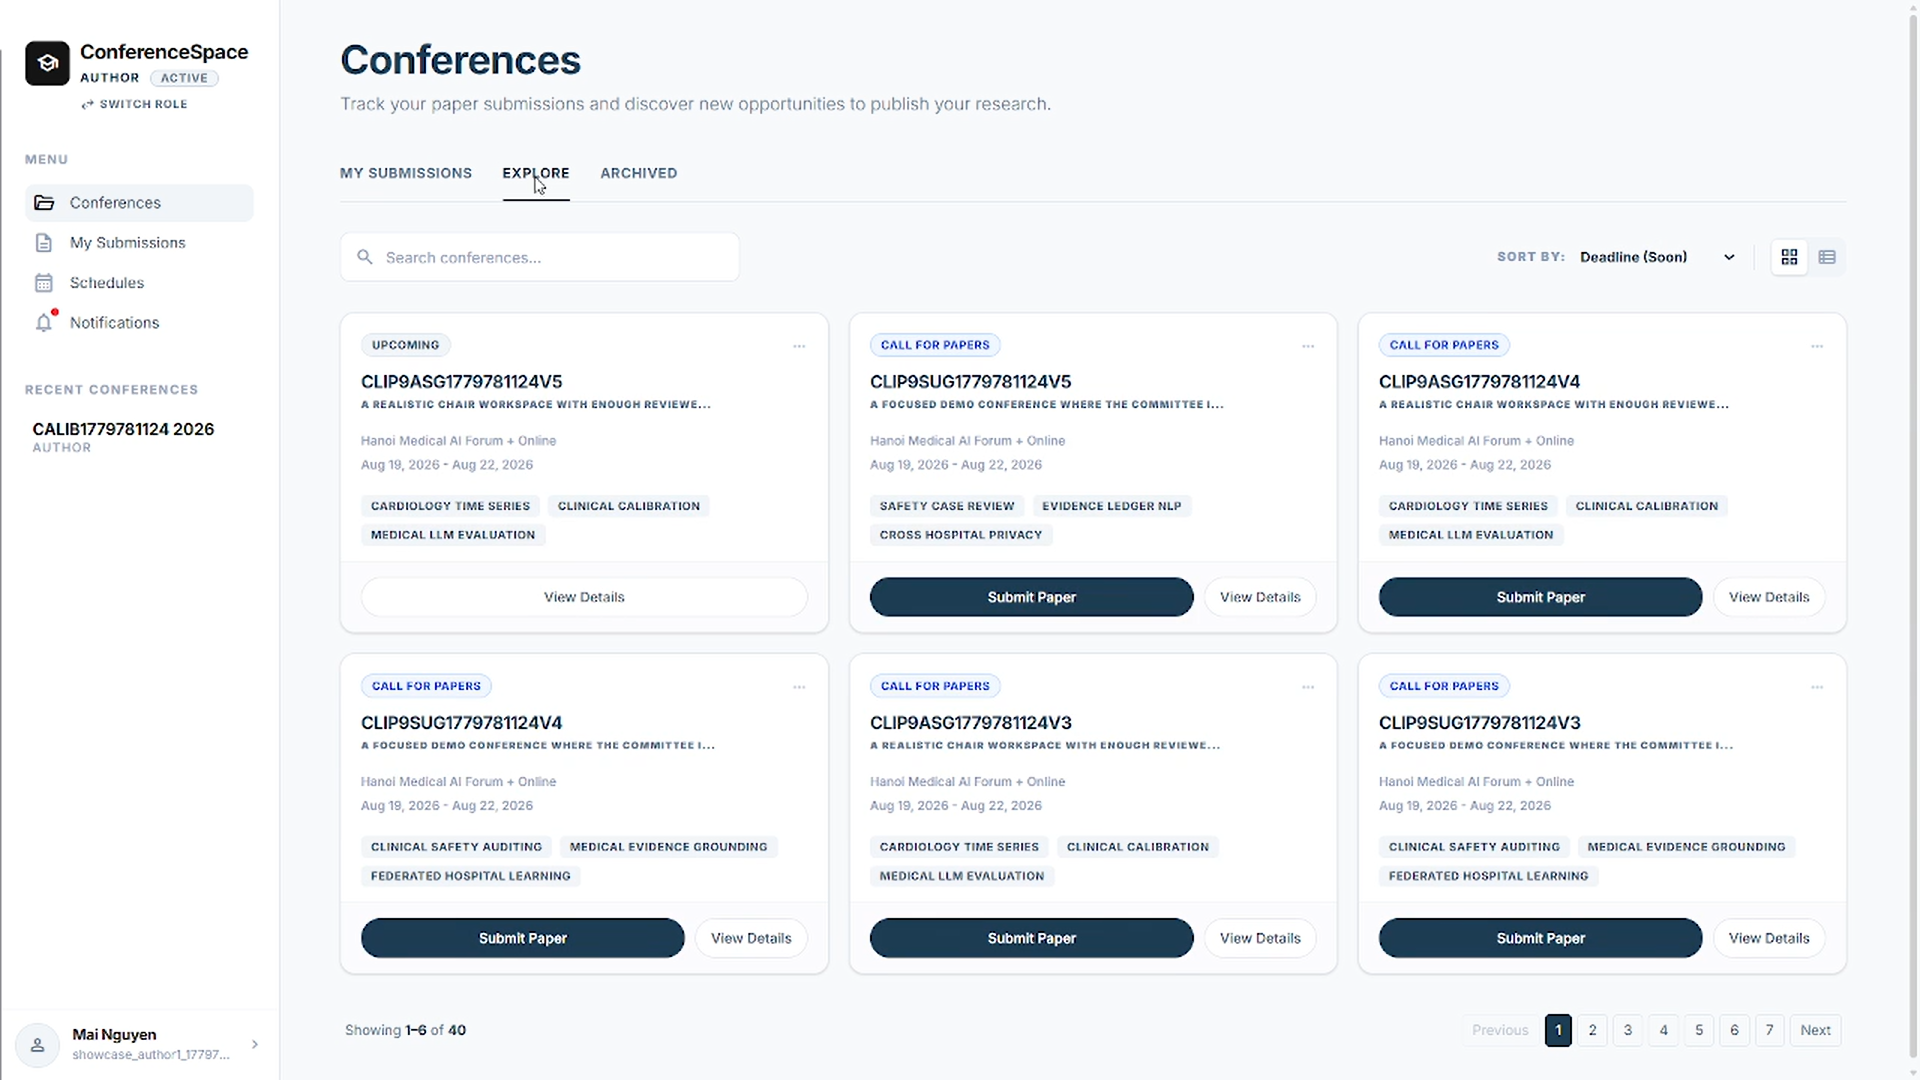
\includegraphics[width=0.95\textwidth]{images/chapter_3_uc01_explore_conferences.png}
  \caption{Giao diện khám phá danh sách hội nghị mặc định}
  \label{fig:uc01-explore-cut}
\end{figure}

Hình~\ref{fig:uc01-explore-cut} minh họa giao diện danh sách hội nghị mặc định mà Tác giả nhìn thấy khi bắt đầu tìm kiếm.

\begin{figure}[H]
  \centering
  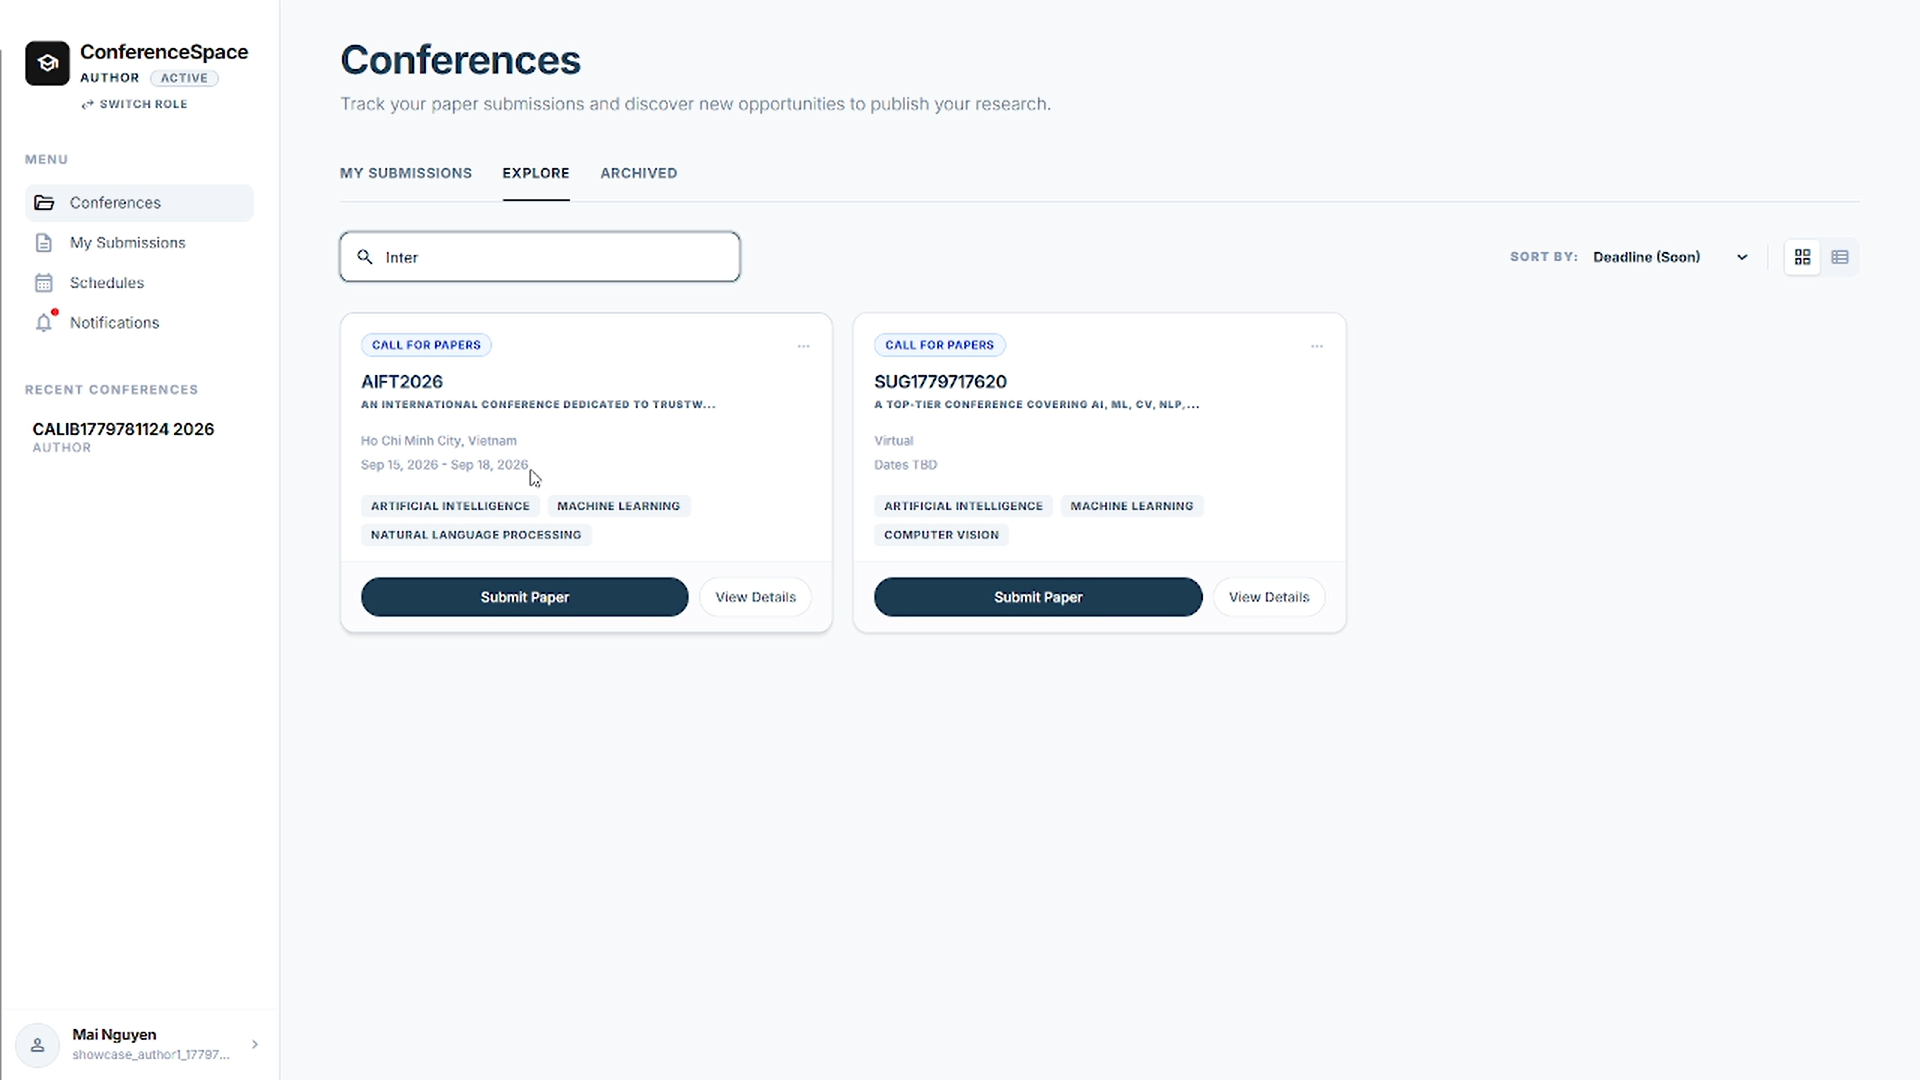
\includegraphics[width=0.95\textwidth]{images/chapter_3_uc01_search_conferences.png}
  \caption{Kết quả tìm kiếm và áp dụng bộ lọc động}
  \label{fig:uc01-search-cut}
\end{figure}

Hình~\ref{fig:uc01-search-cut} minh họa kết quả tìm kiếm sau khi Tác giả áp dụng bộ lọc động.

\begin{figure}[H]
  \centering
  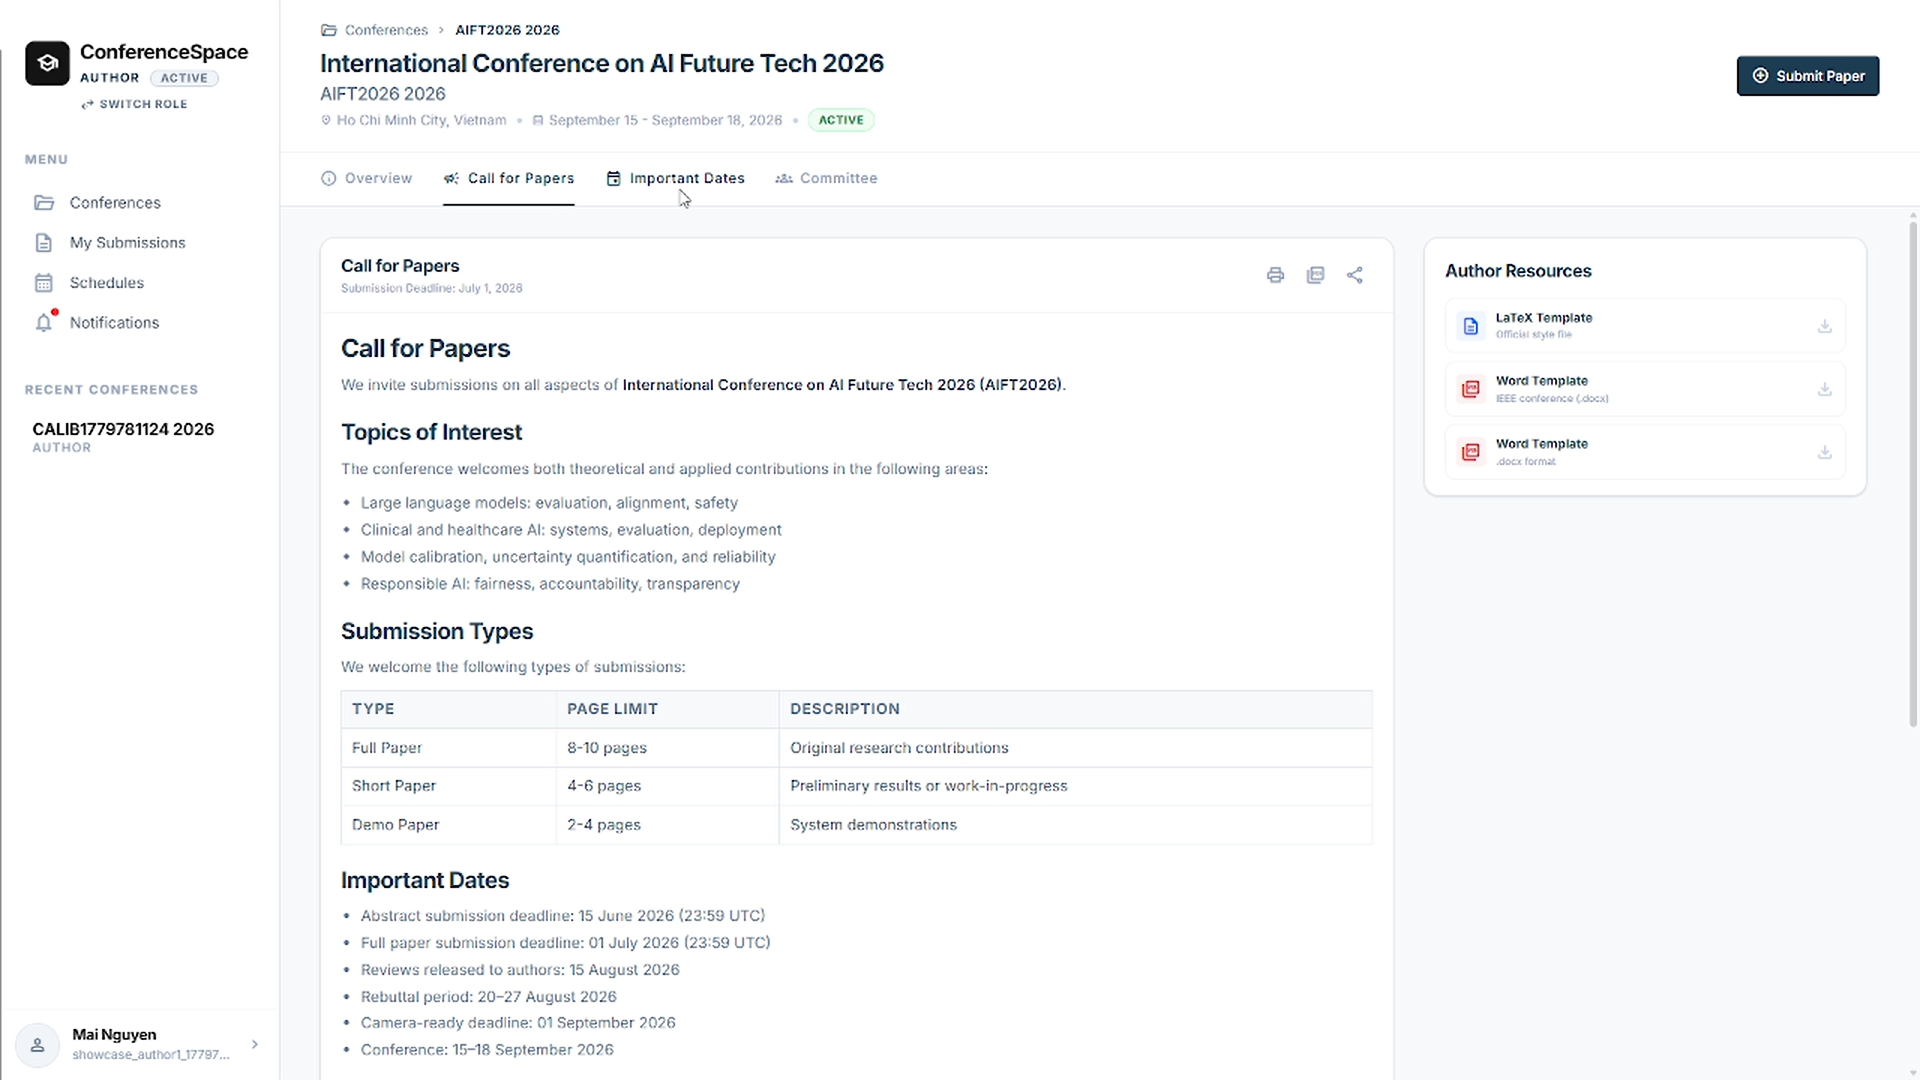
\includegraphics[width=0.95\textwidth]{images/chapter_3_uc01_conference_detail_cfp.png}
  \caption{Giao diện trang chi tiết hội nghị: Tab kêu gọi nộp bài (Call for Papers)}
  \label{fig:uc01-detail-cfp-cut}
\end{figure}

Hình~\ref{fig:uc01-detail-cfp-cut} thể hiện tab kêu gọi nộp bài (Call for Papers) trên trang chi tiết hội nghị.

\begin{figure}[H]
  \centering
  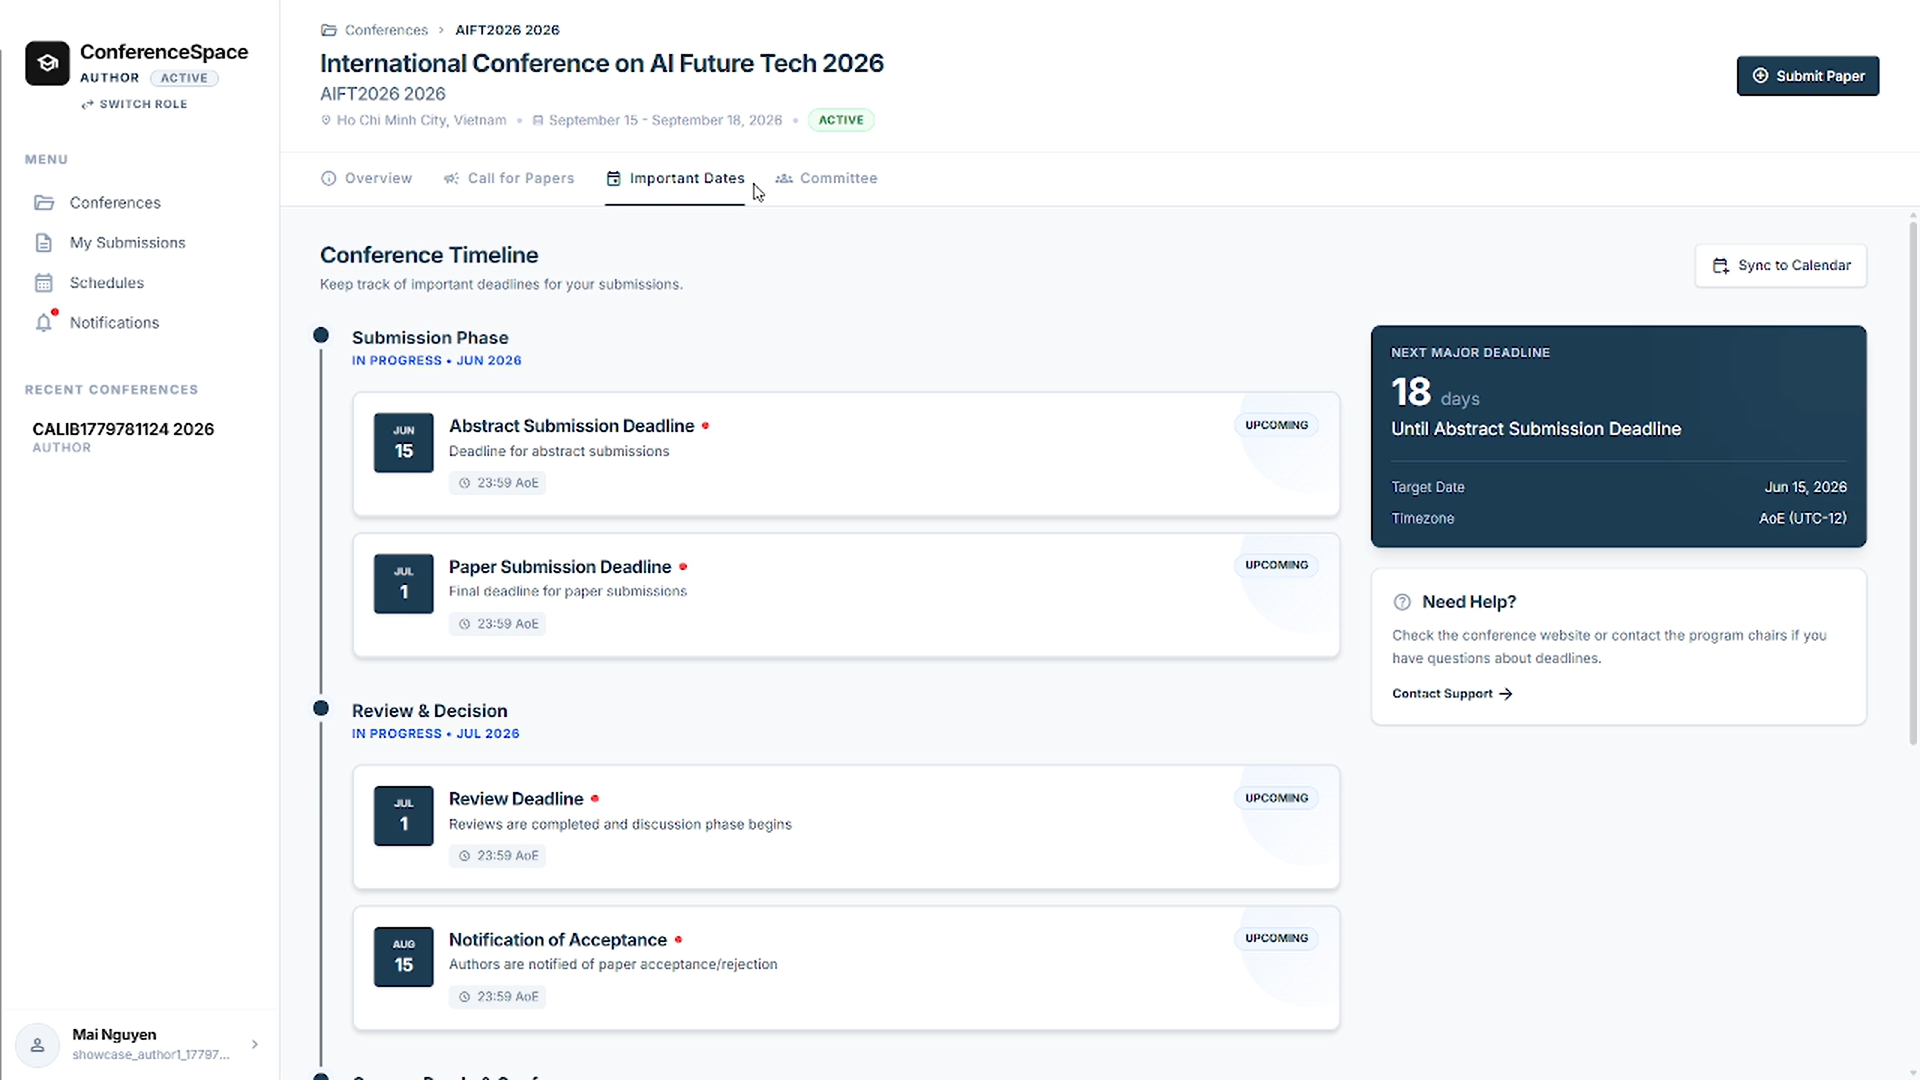
\includegraphics[width=0.95\textwidth]{images/chapter_3_uc01_conference_detail_dates.png}
  \caption{Giao diện trang chi tiết hội nghị: Tab mốc thời gian quan trọng (Important Dates)}
  \label{fig:uc01-detail-dates-cut}
\end{figure}


Hình~\ref{fig:uc01-detail-dates-cut} thể hiện tab mốc thời gian quan trọng trên trang chi tiết hội nghị.

\begin{figure}[H]
  \centering
  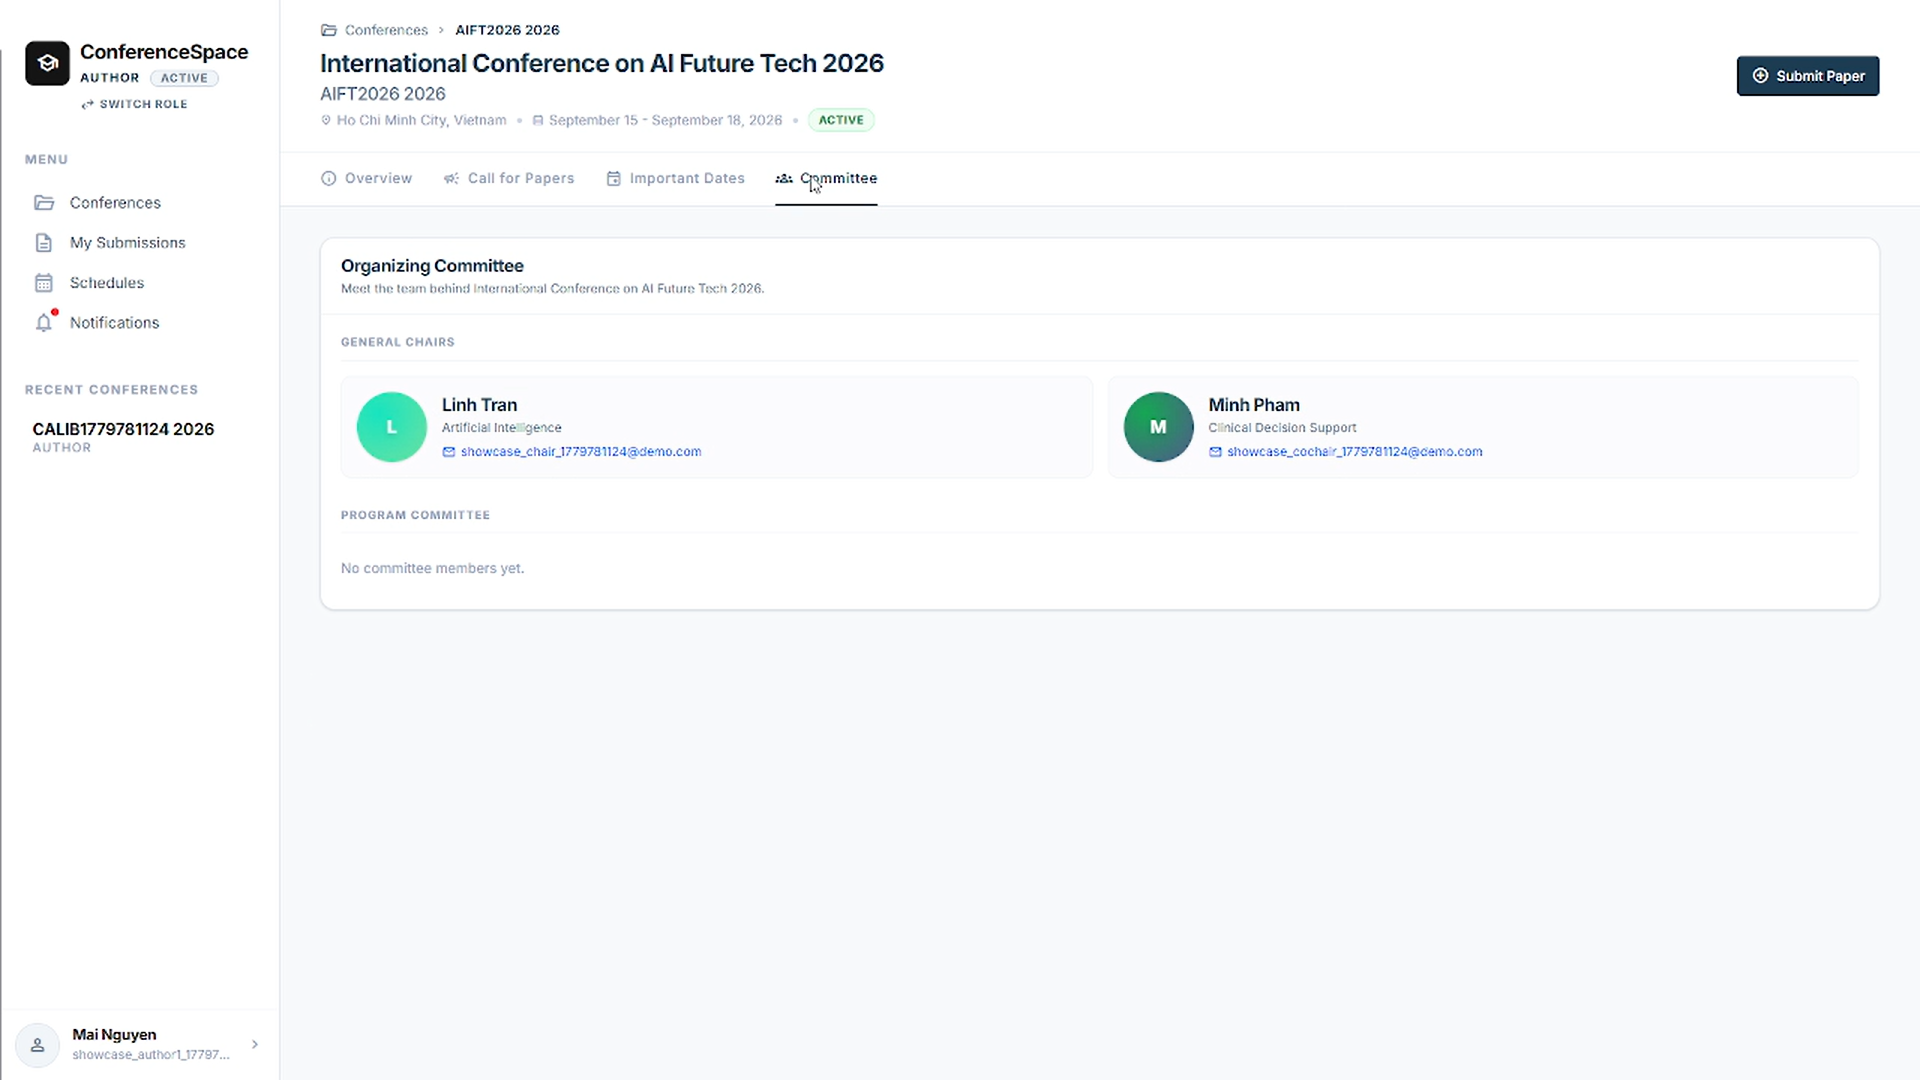
\includegraphics[width=0.95\textwidth]{images/chapter_3_uc01_conference_detail_committee.png}
  \caption{Giao diện trang chi tiết hội nghị: tab hội đồng chương trình (Committee)}
  \label{fig:uc01-detail-committee-cut}
\end{figure}

Hình~\ref{fig:uc01-detail-committee-cut} thể hiện tab hội đồng chương trình trên trang chi tiết hội nghị.

\begin{figure}[H]
  \centering
  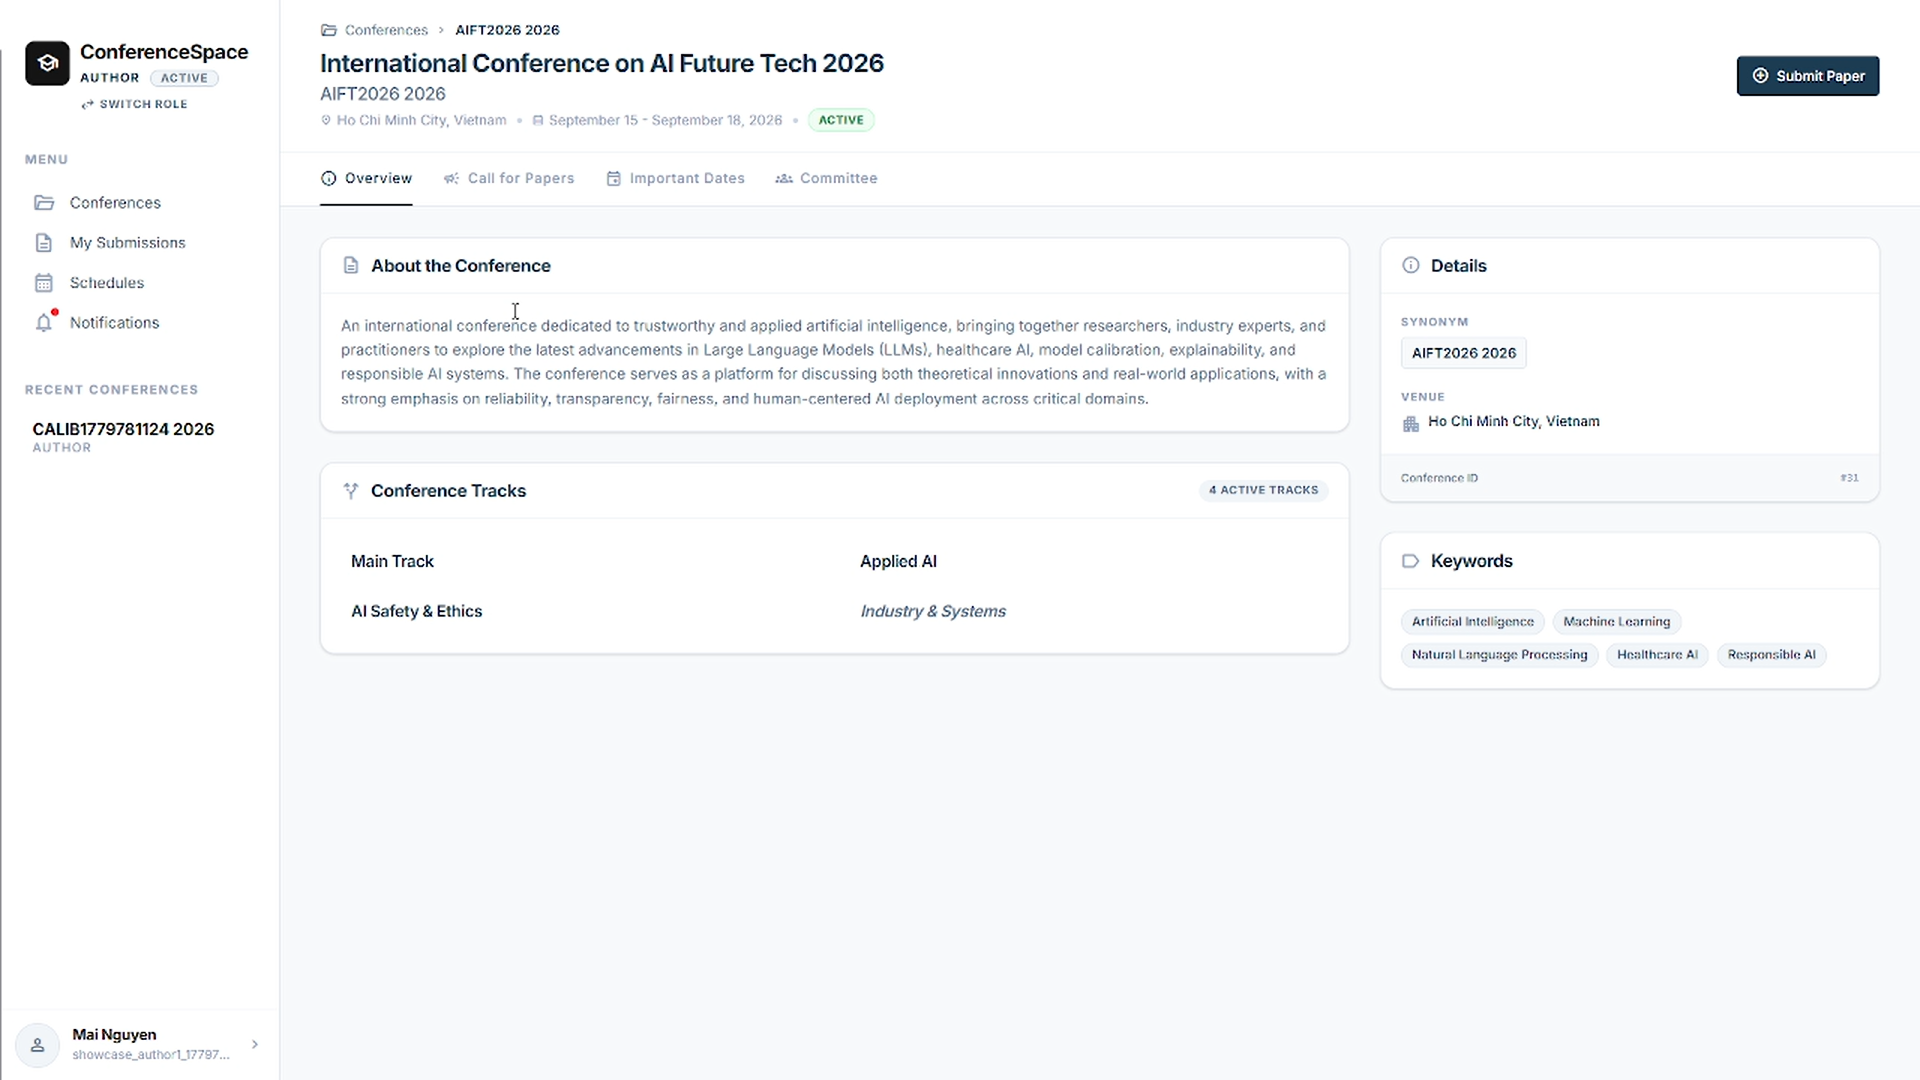
\includegraphics[width=0.95\textwidth]{images/chapter_3_uc01_conference_detail_overview.png}
  \caption{Giao diện trang chi tiết hội nghị: Tab tổng quan (Overview)}
  \label{fig:uc01-detail-overview-cut}
\end{figure}

Hình~\ref{fig:uc01-detail-overview-cut} thể hiện tab tổng quan của trang chi tiết hội nghị mà Tác giả xem trước khi quyết định nộp bài hoặc lưu theo dõi.

\subsubsection{UC-02. Hoàn tất và kiểm tra bài nộp}

Tác giả tạo bản nháp, tải bản thảo và có thể yêu cầu Submission Autofill trích xuất siêu dữ liệu cùng gợi ý chuyên đề trong danh sách hợp lệ. Tác giả kiểm tra, chỉnh sửa thông tin, khai báo đồng tác giả và xung đột lợi ích trước khi Submission Gating kiểm tra tệp, chính sách và các điều kiện gửi bài. Trạng thái \textit{warn} cho phép tiếp tục khi chính sách hội nghị cho phép; trạng thái \textit{block} ngăn gửi cho đến khi lỗi có căn cứ được khắc phục. Nếu Submission Autofill không khả dụng, Tác giả vẫn có thể nhập và lưu bản nháp thủ công. Nếu Submission Gating không trả được bất kỳ kết quả hợp lệ nào, backend chưa cho phép gửi bài cho đến khi thực hiện được một lần kiểm tra hợp lệ.

\begin{figure}[H]
  \centering
  \begin{minipage}{0.48\textwidth}
    \centering
    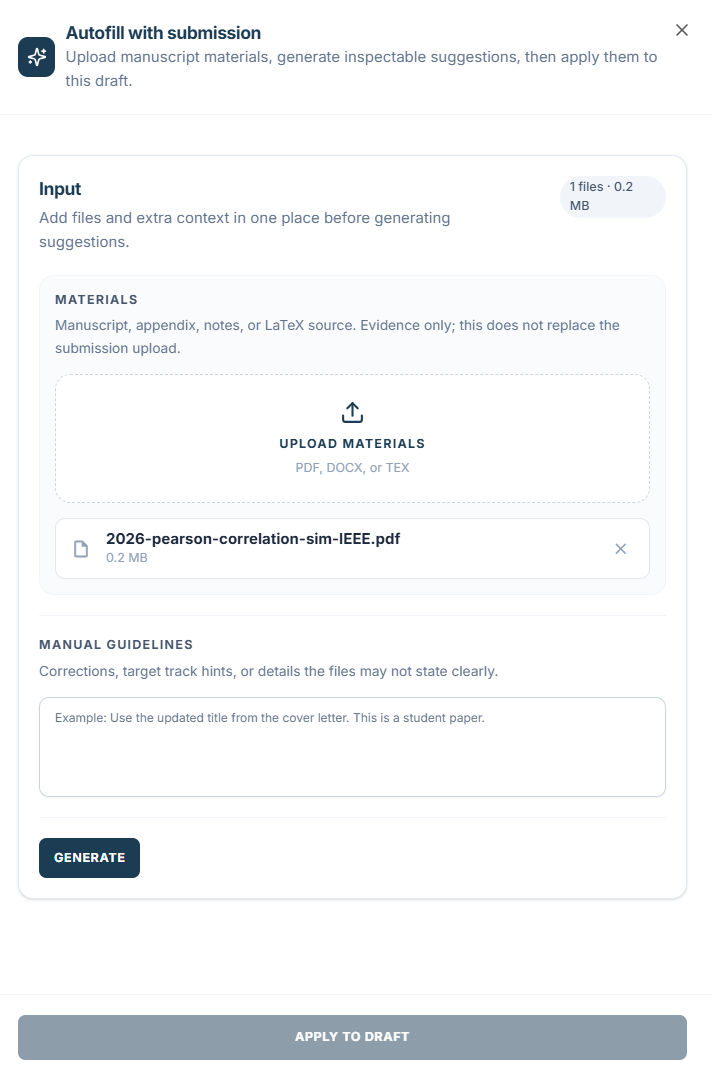
\includegraphics[width=0.56\textwidth]{images/chapter_3_uc02_autofill_1.png}
  \end{minipage}
  \begin{minipage}{0.48\textwidth}
    \centering
    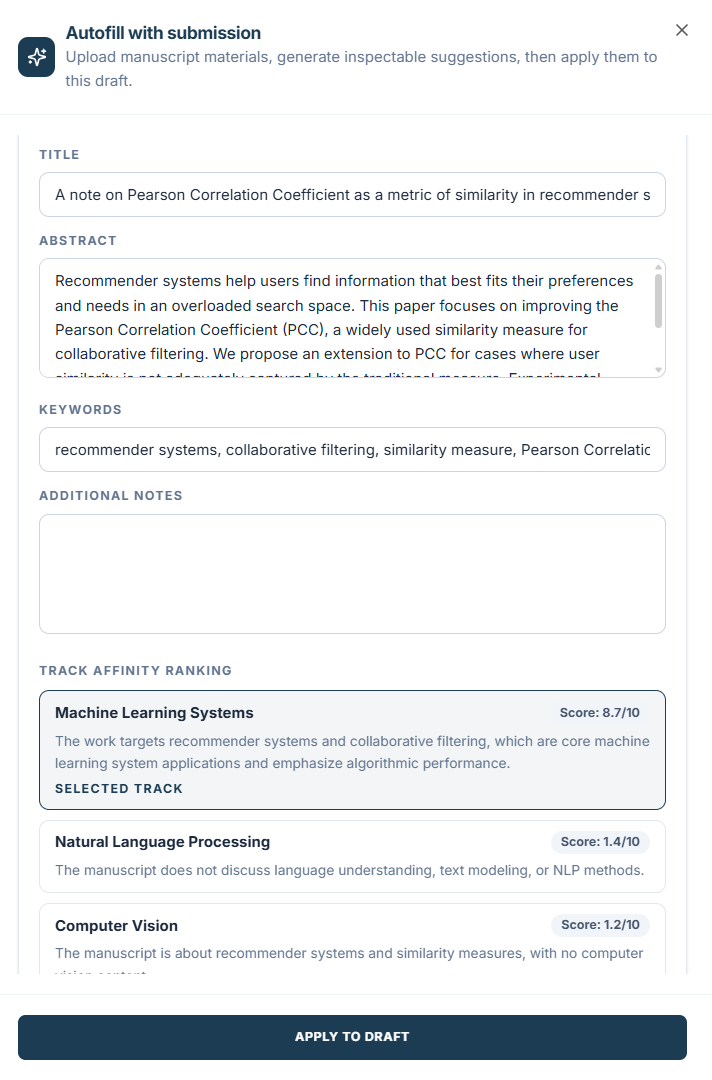
\includegraphics[width=0.56\textwidth]{images/chapter_3_uc02_autofill_2.png}
  \end{minipage}
  \caption{Giao diện tải lên bản thảo (trái) và kết quả trích xuất thông tin tự động (phải)}
  \label{fig:uc02-autofill-cut}
\end{figure}

Hình~\ref{fig:uc02-autofill-cut} trình bày giao diện tải lên bản thảo (trái) cùng kết quả trích xuất thông tin mà Submission Autofill trả về (phải) để Tác giả kiểm tra và chỉnh sửa.

\begin{figure}[H]
  \centering
  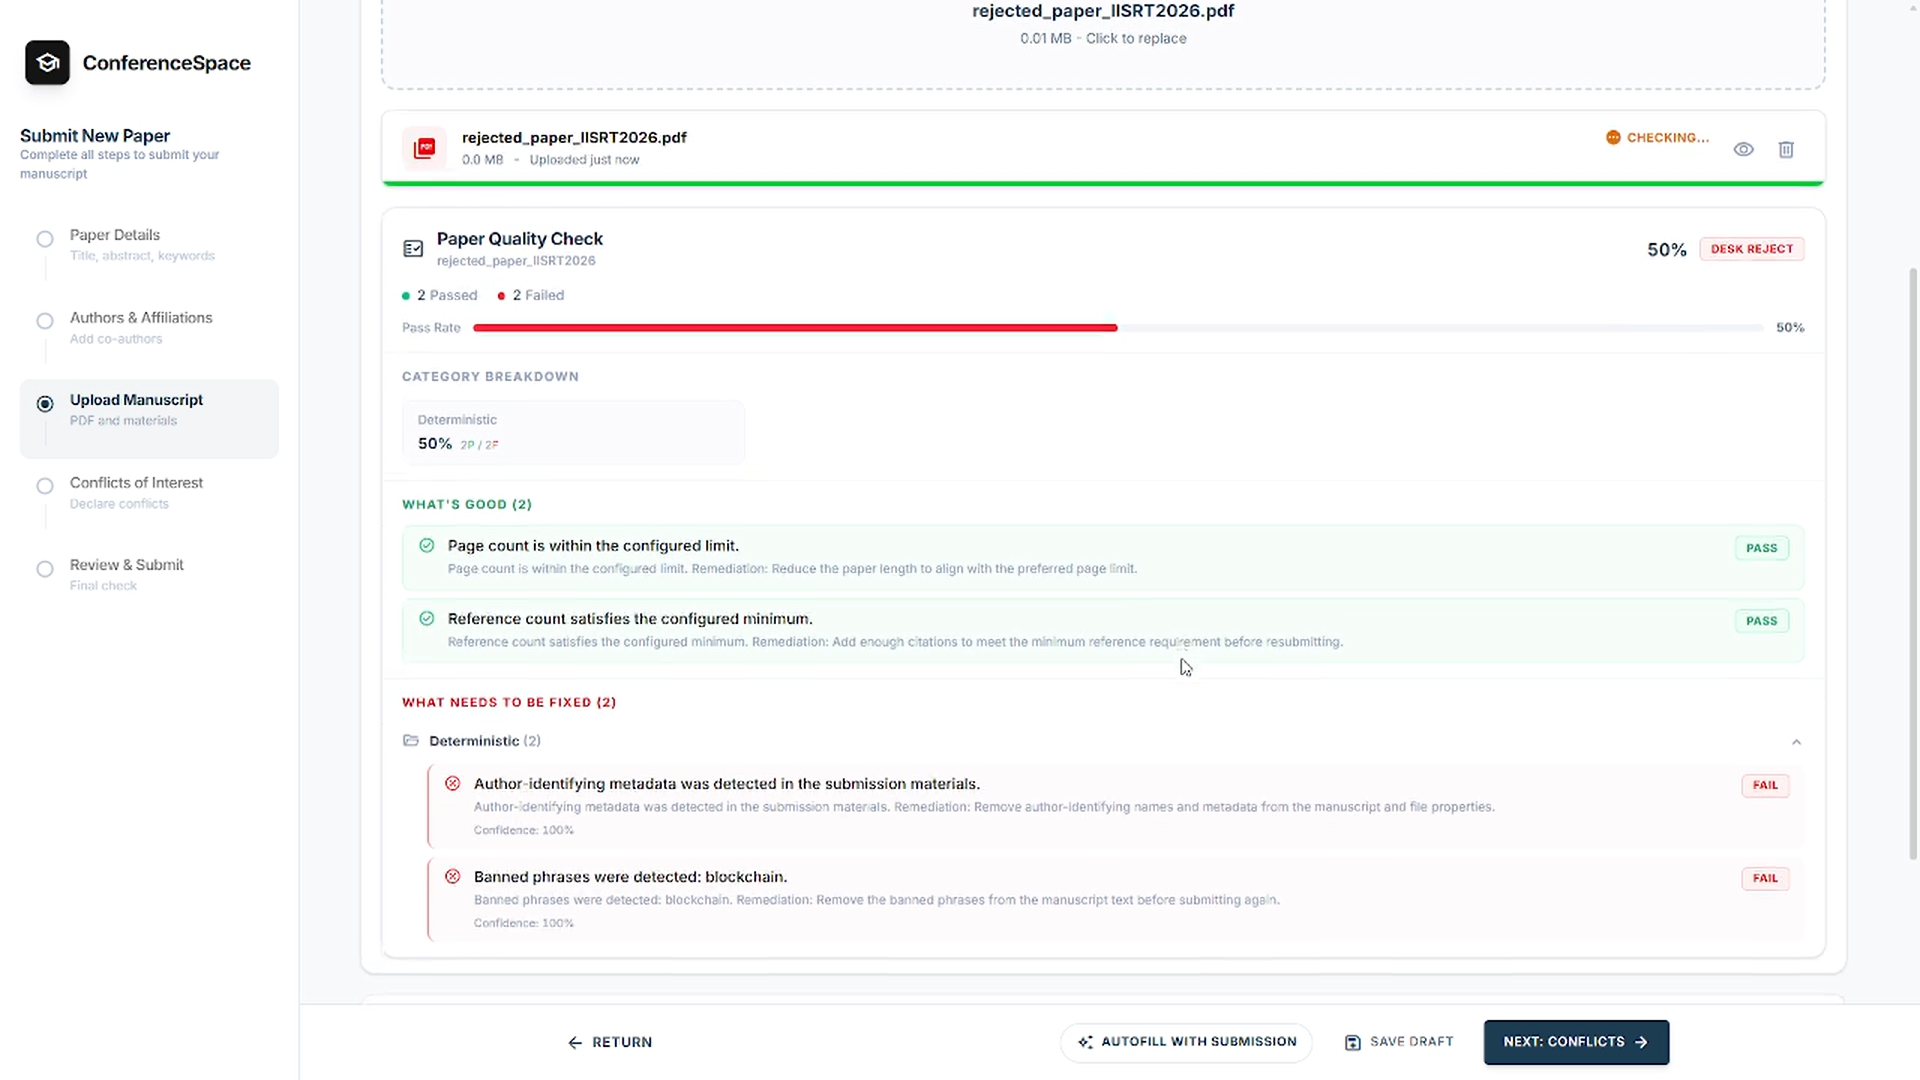
\includegraphics[width=0.95\textwidth]{images/chapter_3_uc02_precheck_gating.png}
  \caption{Kết quả Submission Gating theo ba trạng thái \textit{pass}, \textit{warn} và \textit{block}}
  \label{fig:uc02-gating-cut}
\end{figure}

Trước khi gửi bài, Tác giả xem kết quả kiểm tra tự động của Submission Gating tại Hình~\ref{fig:uc02-gating-cut}, gồm ba trạng thái \textit{pass}, \textit{warn} và \textit{block}.

\begin{figure}[H]
  \centering
  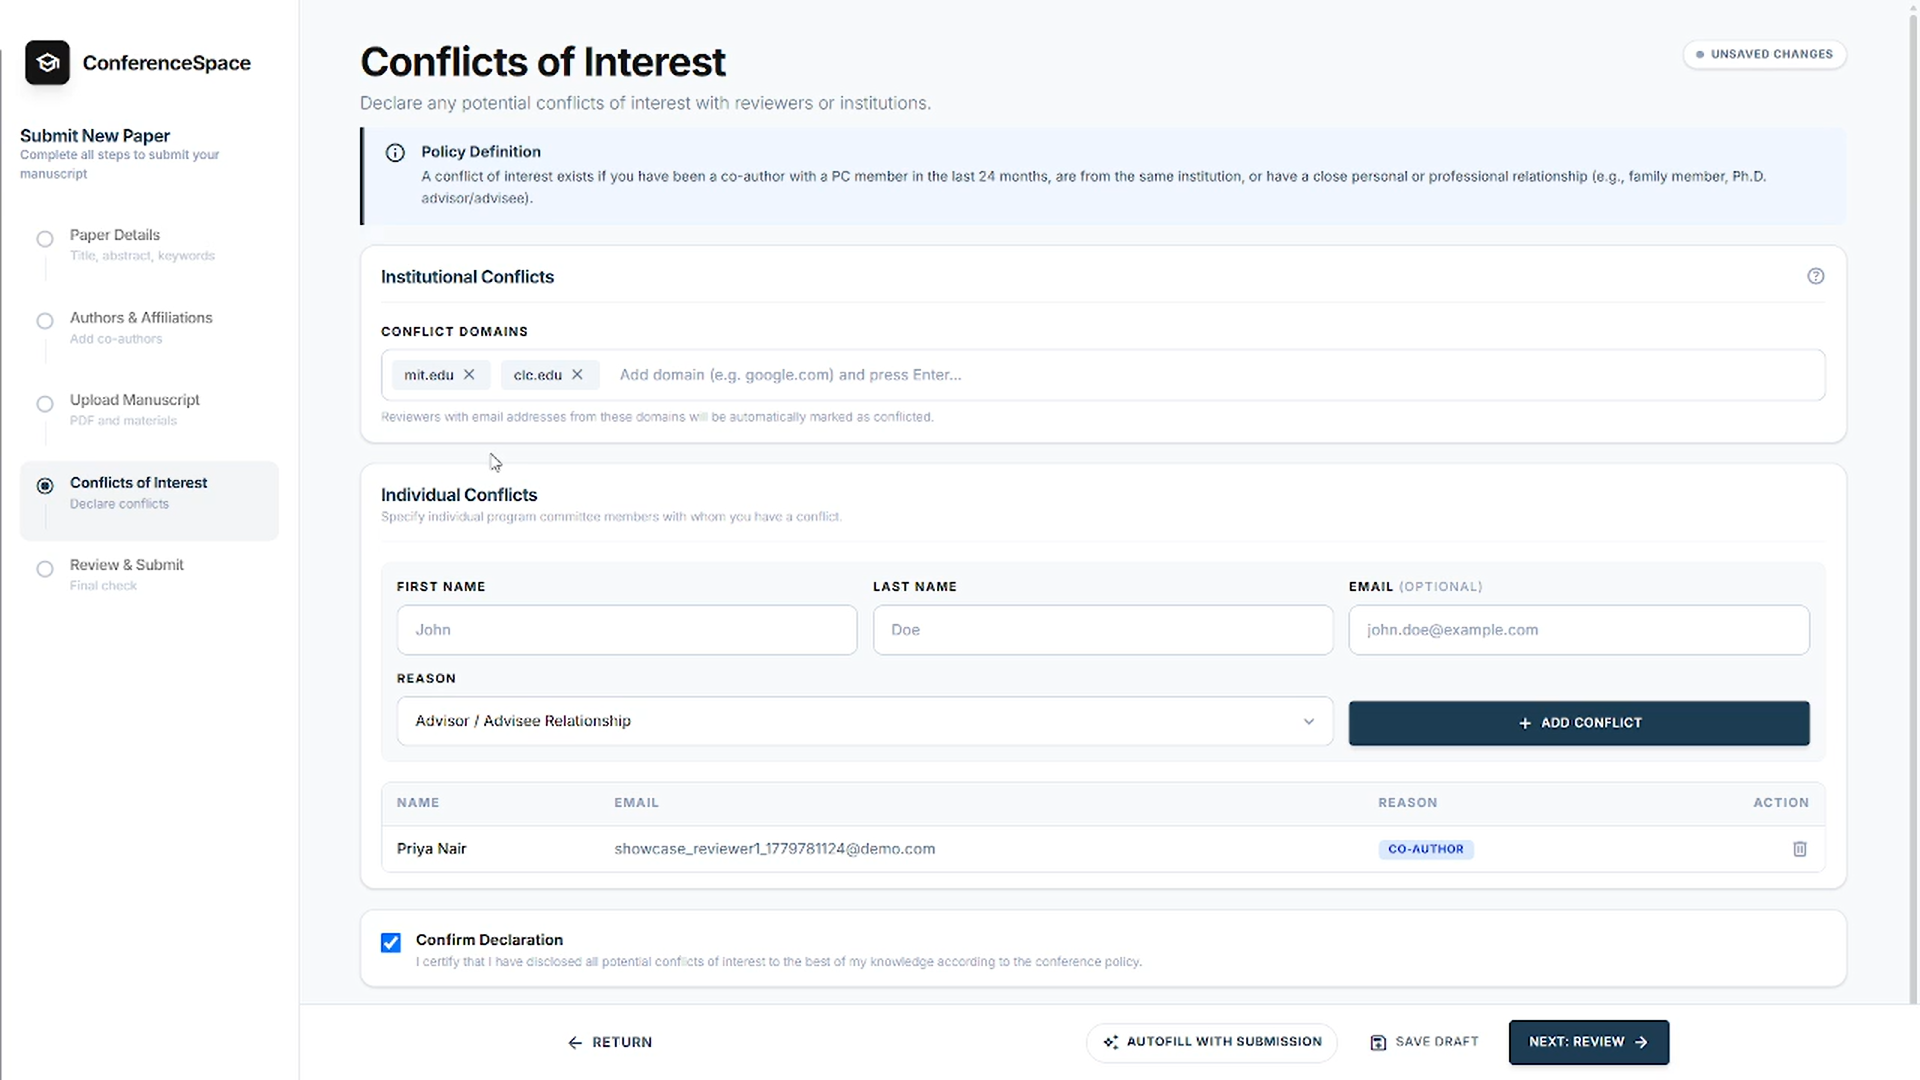
\includegraphics[width=0.95\textwidth]{images/chapter_3_uc02_authors_conflict.png}
  \caption{Giao diện khai báo thông tin các đồng tác giả và xung đột lợi ích}
  \label{fig:uc02-authors-conflict-cut}
\end{figure}

Hình~\ref{fig:uc02-authors-conflict-cut} minh họa giao diện khai báo đồng tác giả và xung đột lợi ích mà Tác giả hoàn tất trước khi Submission Gating kiểm tra.

Hai chức năng AI chỉ hỗ trợ hoàn tất bài nộp: Submission Autofill tạo bản nháp có thể sửa, còn Submission Gating kiểm tra điều kiện trước khi gửi. Tác giả vẫn là người xác nhận dữ liệu và thực hiện thao tác gửi chính thức.

\subsubsection{UC-03. Quản lý vòng đời bài nộp}

Sau khi tạo bài, Tác giả theo dõi và thực hiện các hành động phù hợp với từng trạng thái: chỉnh sửa bản nháp; theo dõi hoặc rút bài đã gửi khi cấu hình và hạn chót nộp bài cho phép; xem phản biện khi được công bố; gửi phản hồi trong giai đoạn do Chủ tọa hoặc Đồng chủ tọa mở; và tải bản thảo hoàn chỉnh khi bài được chấp nhận. Backend từ chối yêu cầu không phù hợp với trạng thái hoặc hạn chót tương ứng. Phiên bản hiện tại hỗ trợ tải và truy xuất bản thảo hoàn chỉnh nhưng chưa có luồng để Chủ tọa phê duyệt, yêu cầu nộp lại hoặc kiểm tra hạn chót nộp bản thảo hoàn chỉnh tại thời điểm thực thi.

\begin{figure}[H]
  \centering
  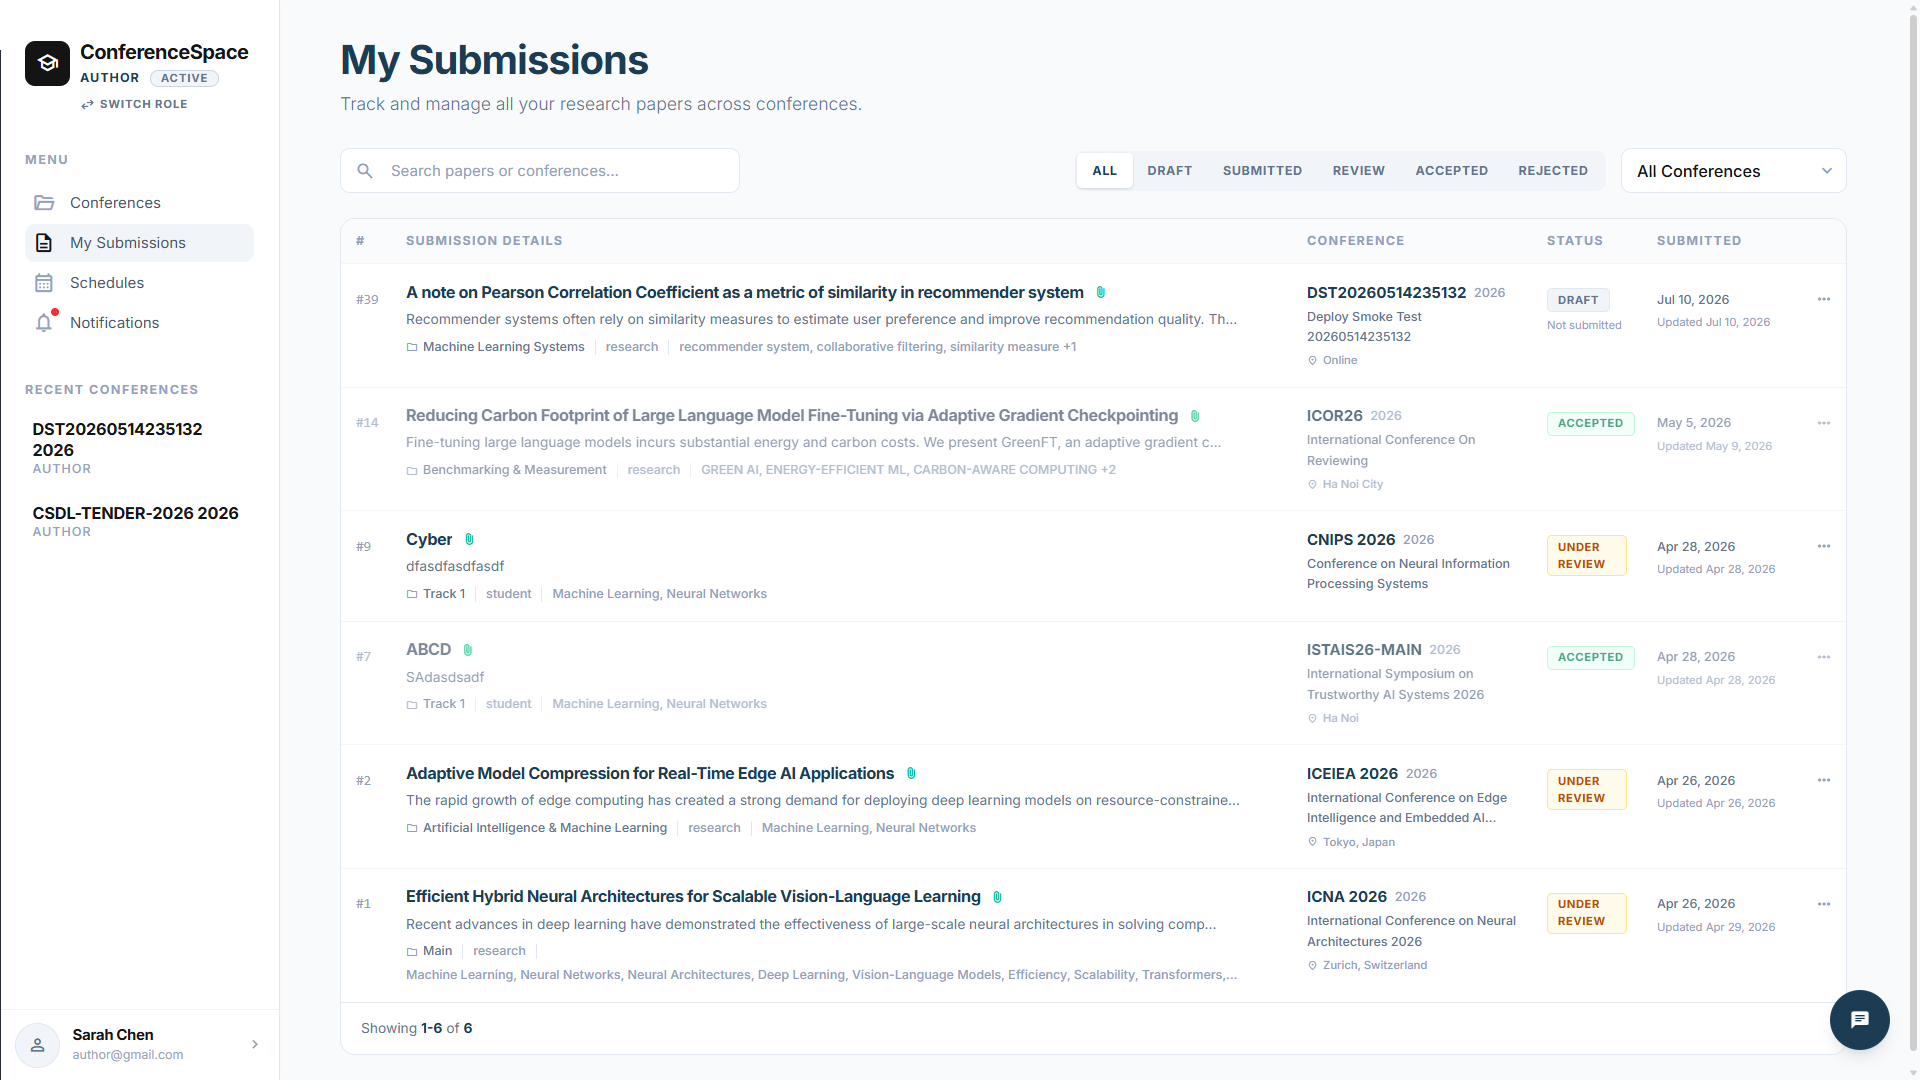
\includegraphics[width=0.95\textwidth]{images/chapter_3_uc03_submissions_list.png}
  \caption{Danh sách bài nộp và trạng thái vòng đời trong không gian làm việc của Tác giả}
  \label{fig:uc03-submissions-cut}
\end{figure}

Giao diện ở Hình~\ref{fig:uc03-submissions-cut} cung cấp một điểm nhìn thống nhất để Tác giả nhận biết trạng thái hiện hành và thao tác nghiệp vụ còn hợp lệ, thay vì chỉ minh họa riêng các chức năng AI ở bước chuẩn bị bài.

\begin{figure}[H]
  \centering
  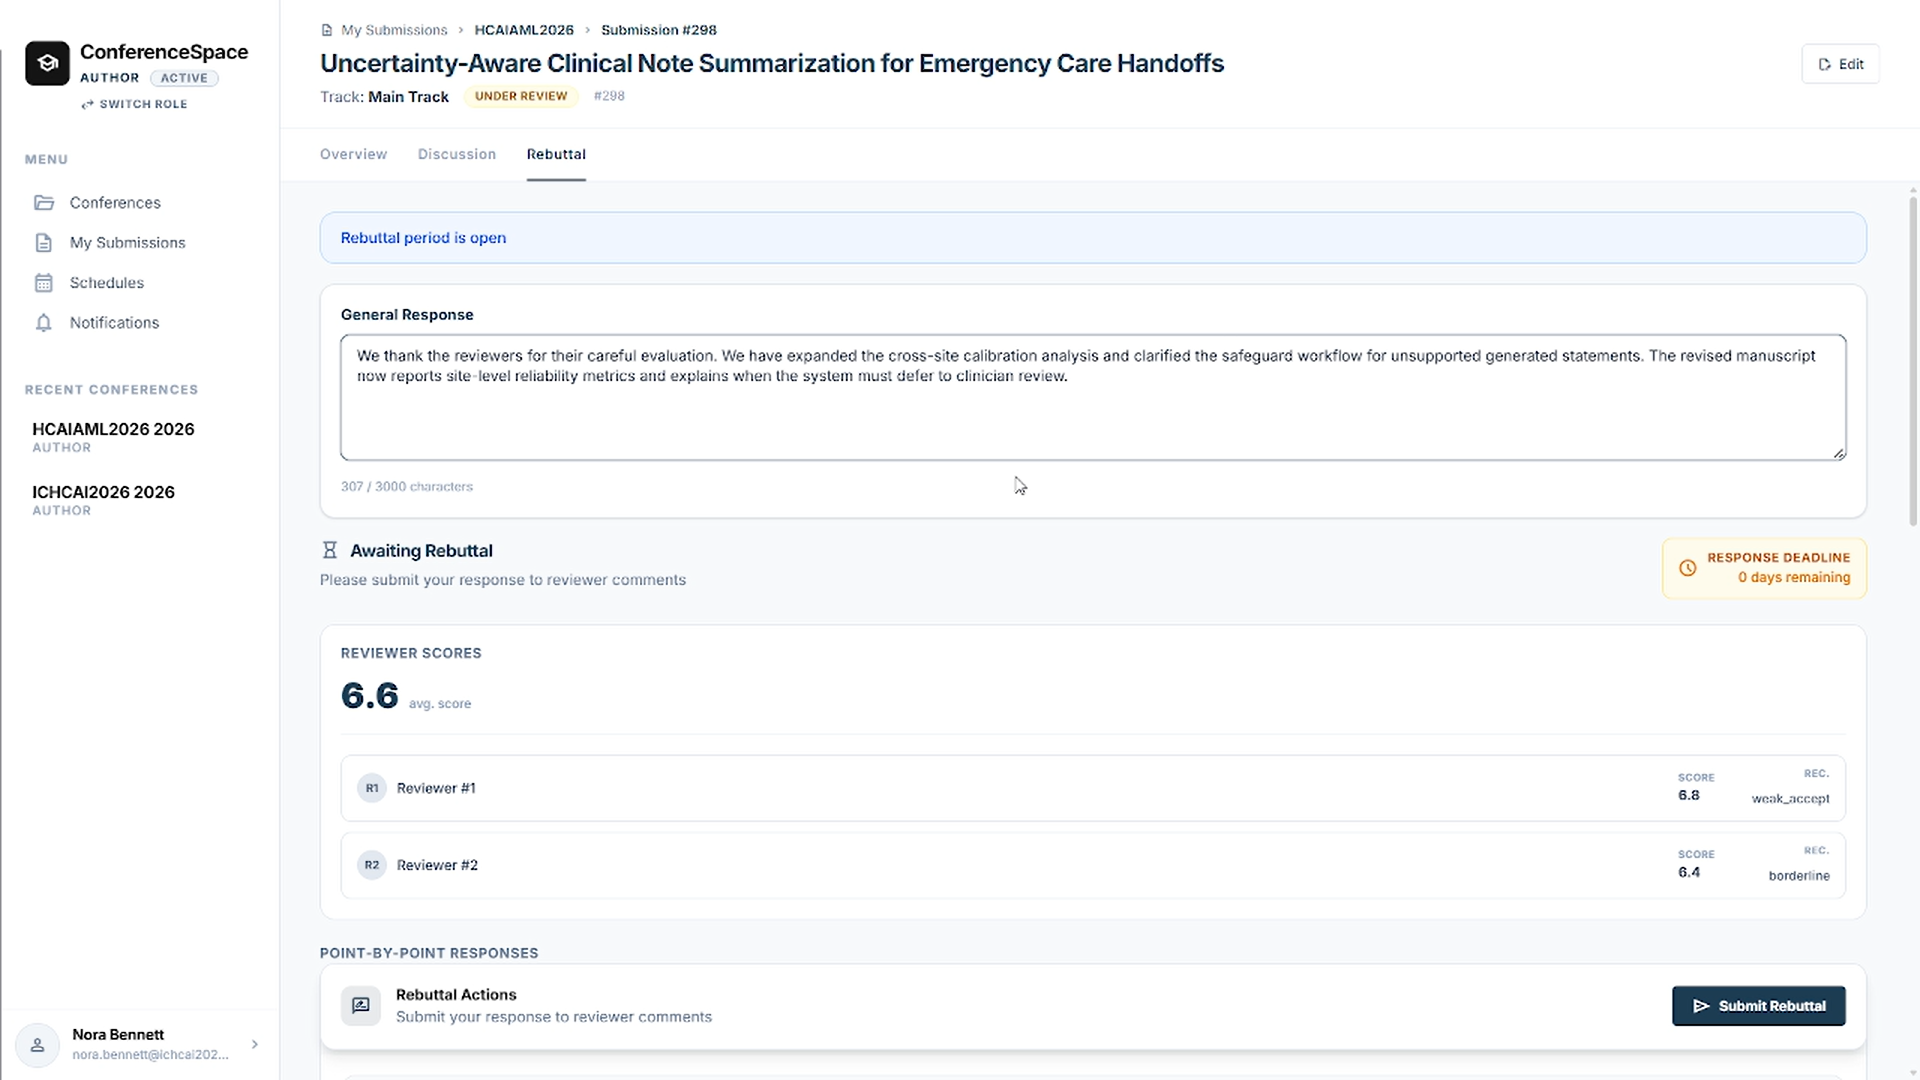
\includegraphics[width=0.95\textwidth]{images/chapter_3_uc03_rebuttal.png}
  \caption{Giao diện soạn thảo và gửi phản hồi của tác giả (rebuttal)}
  \label{fig:uc03-rebuttal-cut}
\end{figure}

Hình~\ref{fig:uc03-rebuttal-cut} minh họa giao diện Tác giả soạn và gửi phản hồi (rebuttal) trong giai đoạn phản hồi.

\begin{figure}[H]
  \centering
  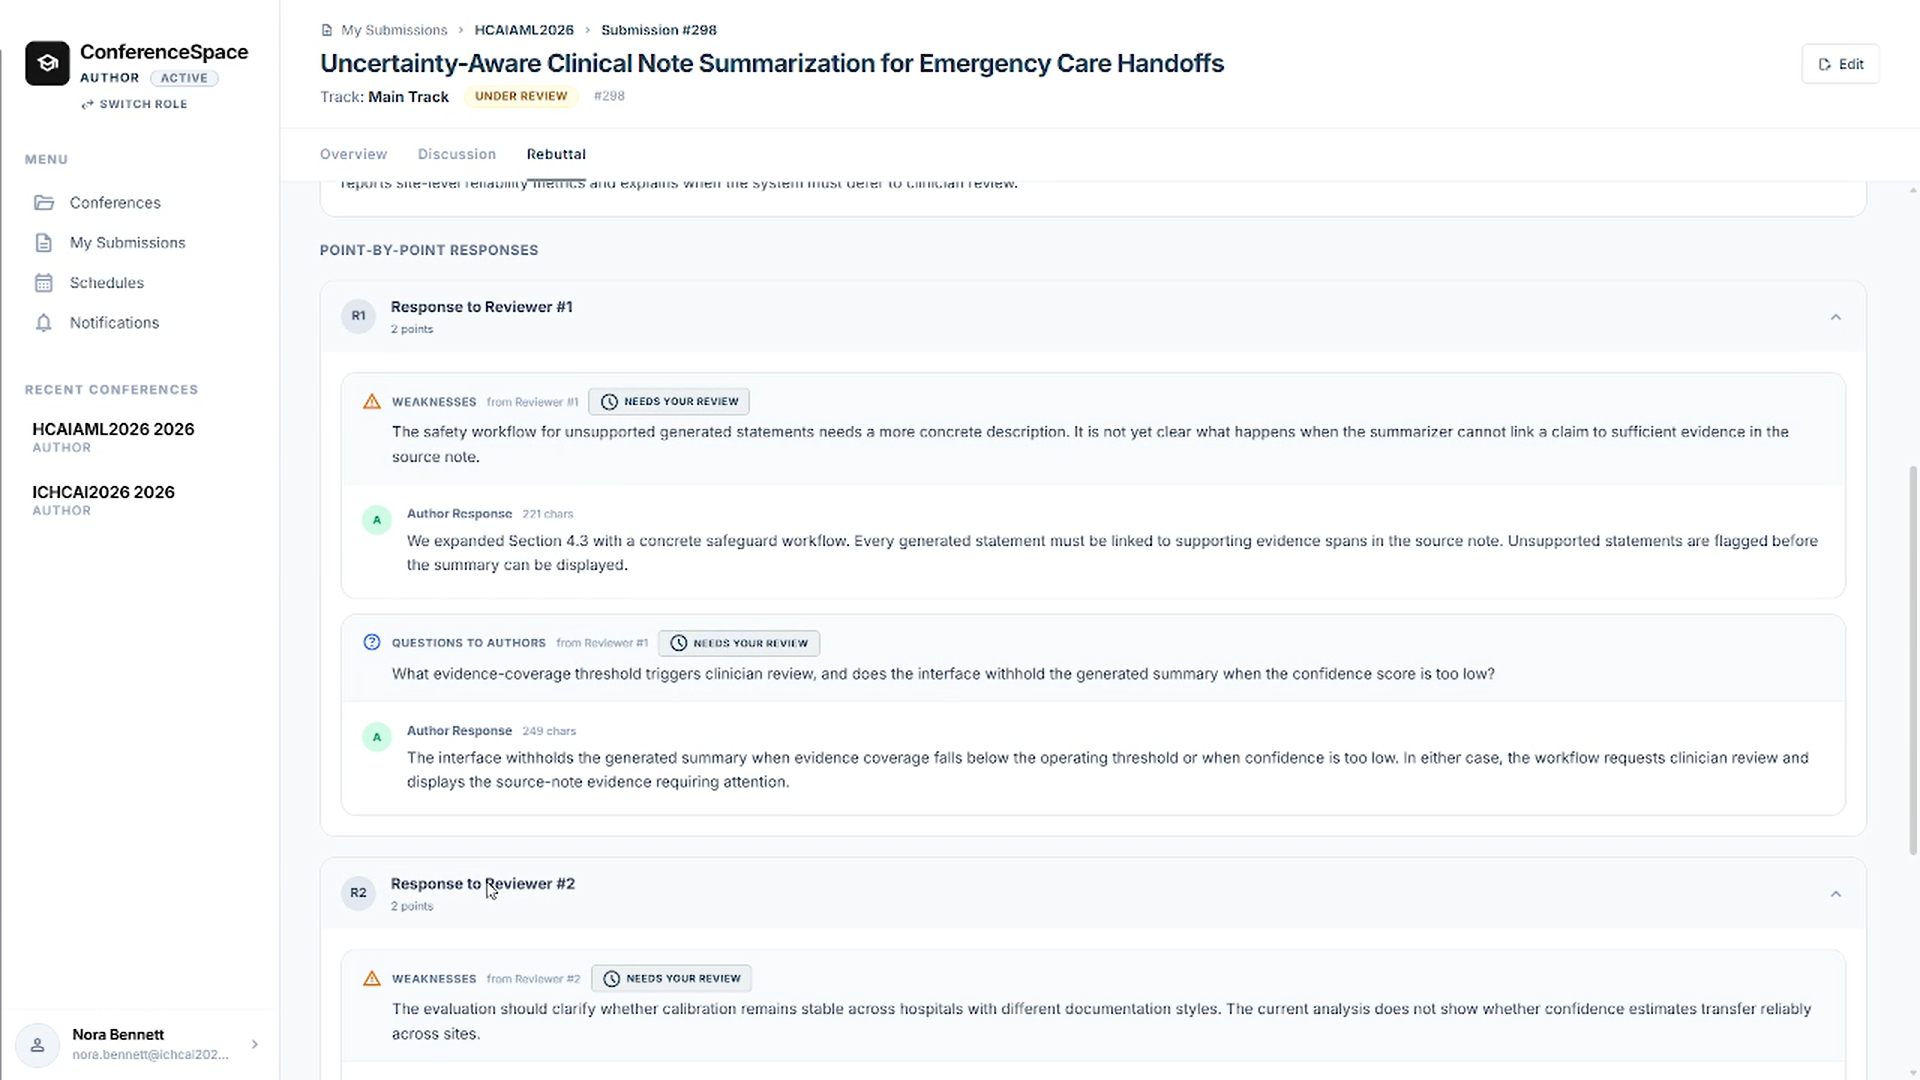
\includegraphics[width=0.95\textwidth]{images/chapter_3_uc03_rebuttal_2.png}
  \caption{Biến thể giao diện soạn và gửi phản hồi của Tác giả (rebuttal)}
  \label{fig:uc03-rebuttal-2-cut}
\end{figure}

Hình~\ref{fig:uc03-rebuttal-2-cut} trình bày một biến thể khác của giao diện soạn thảo và gửi phản hồi.

\begin{figure}[H]
  \centering
  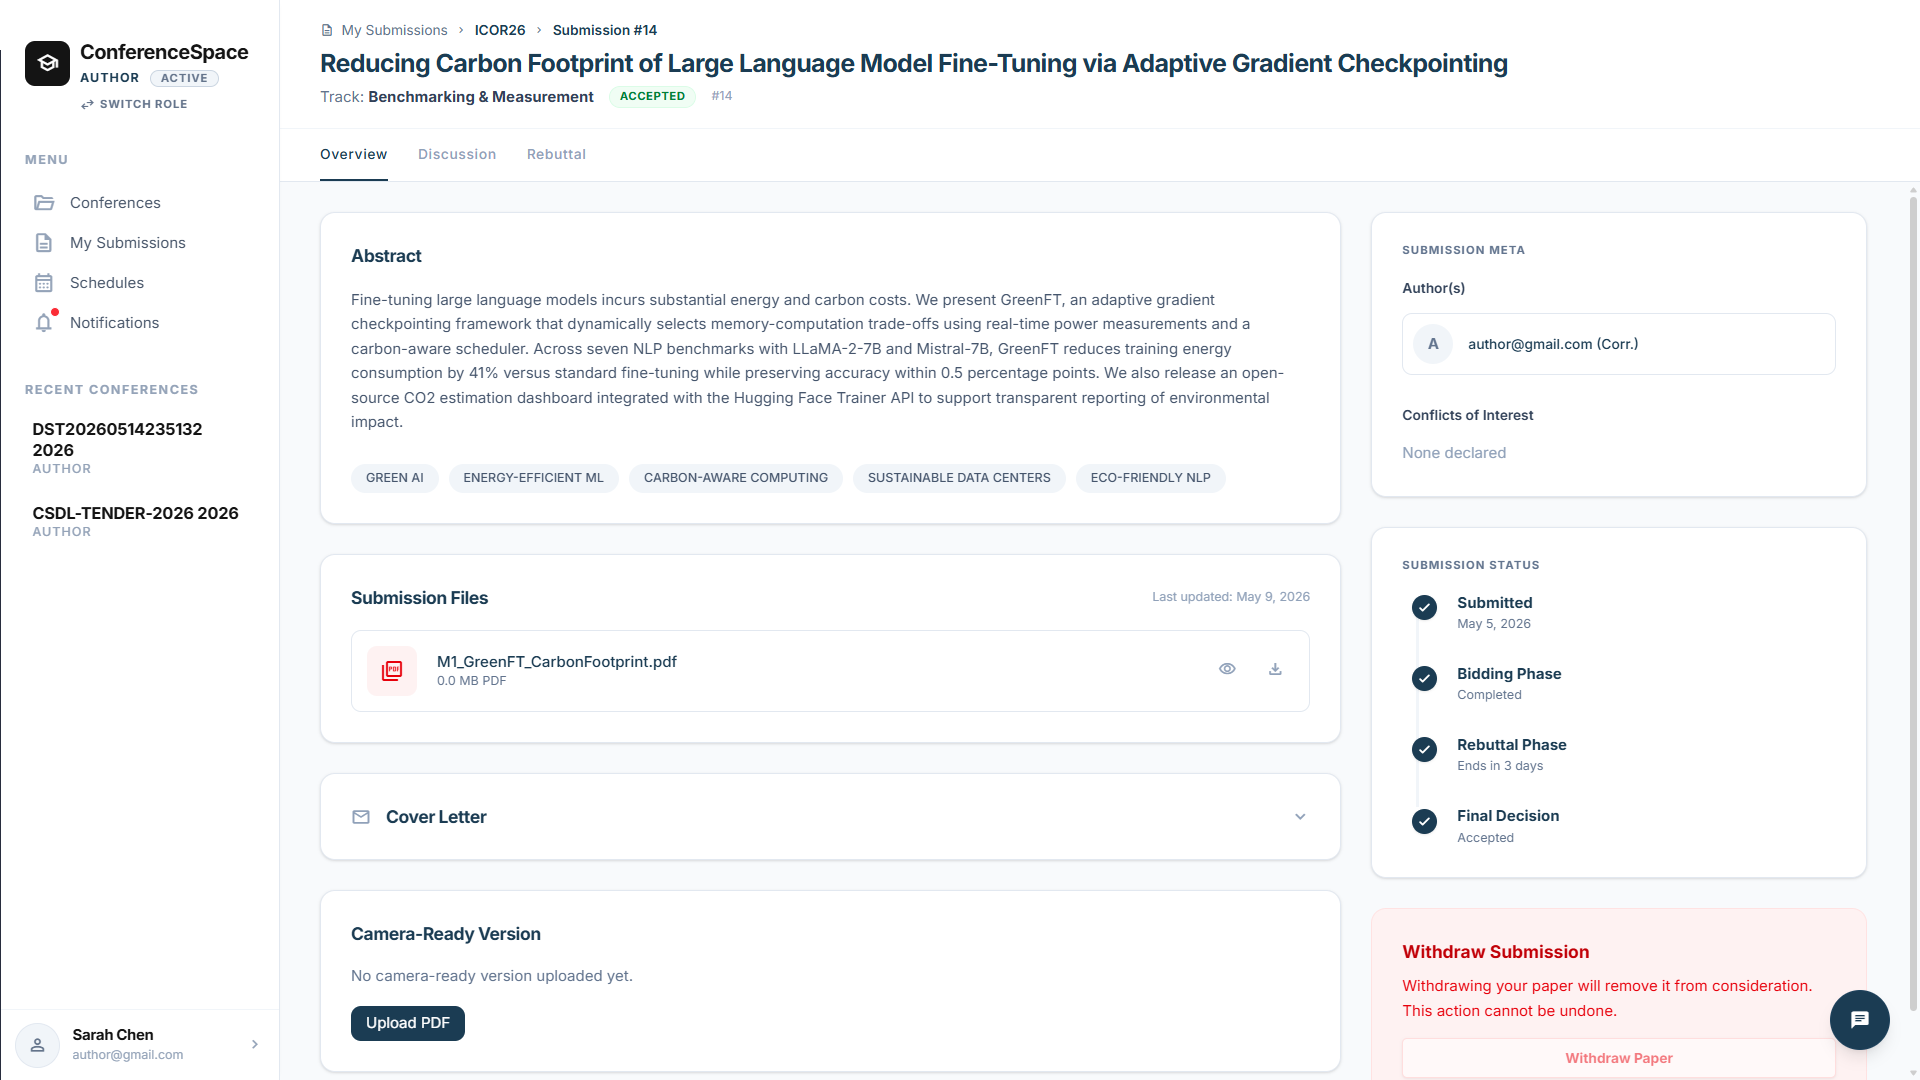
\includegraphics[width=0.95\textwidth]{images/chapter_3_uc03_submission_detail.png}
  \caption{Giao diện trang chi tiết bài nộp, xem nhận định chuyên môn và tải bản thảo hoàn chỉnh (camera-ready)}
  \label{fig:uc03-submission-detail-cut}
\end{figure}

Hình~\ref{fig:uc03-submission-detail-cut} thể hiện trang chi tiết bài nộp, nơi Tác giả xem nhận định chuyên môn và tải lên bản chỉnh sửa cuối cùng khi bài được chấp nhận.

\subsubsection{UC-04. Tiếp nhận lời mời hội nghị và xem bài được phân công}

Chủ tọa gửi lời mời tham gia hội nghị; hệ thống lưu trạng thái và thông báo cho người nhận. Phản biện viên chỉ có thể chấp nhận hoặc từ chối lời mời của chính mình. Đây là trạng thái tham gia hội nghị của Phản biện viên, khác với trạng thái của từng phân công bài. Khi Chủ tọa đã tạo phân công, Phản biện viên xem bài, hạn chót nộp bài và trạng thái trên bảng điều khiển; backend chỉ trả các phân công thuộc người dùng hiện tại. Kho mã nguồn có thao tác phản hồi phân công theo định danh, nhưng luồng giao diện được mô tả trong chương này không đồng nhất thao tác đó với việc chấp nhận lời mời hội nghị.

\begin{figure}[H]
  \centering
  \begin{tabular}{c}
    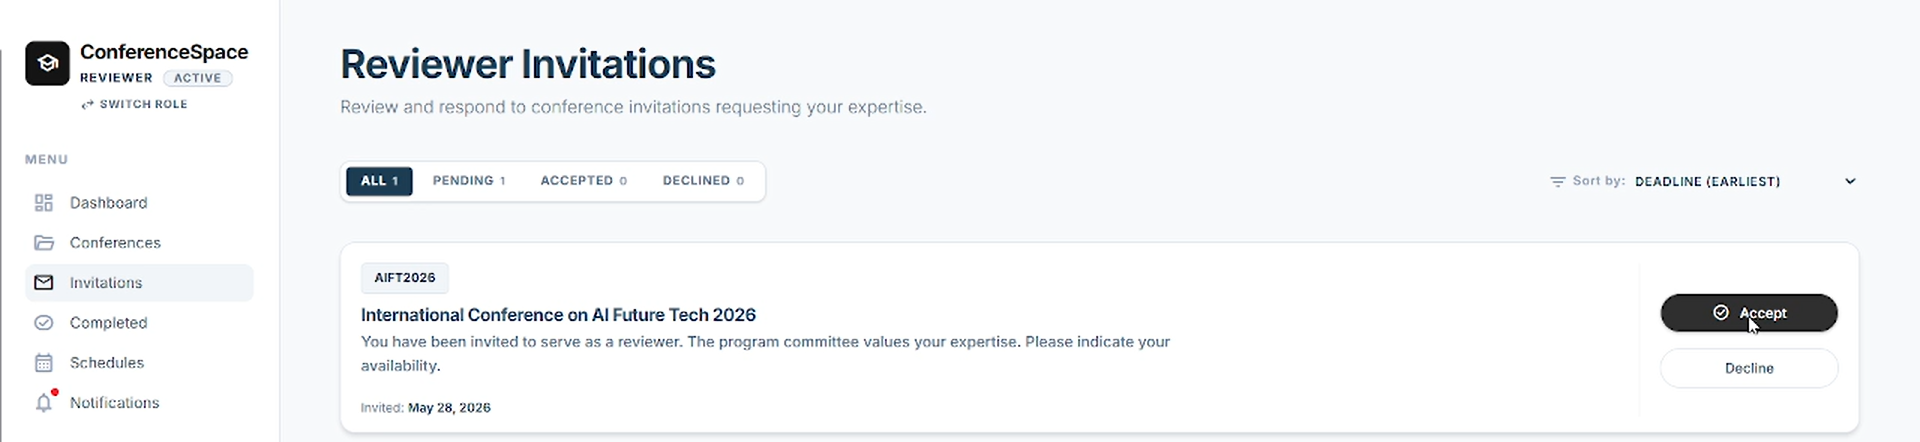
\includegraphics[width=0.95\textwidth]{images/chapter_3_uc04_reviewer_invitations_1.png} \\
    \vspace{0.2cm}
    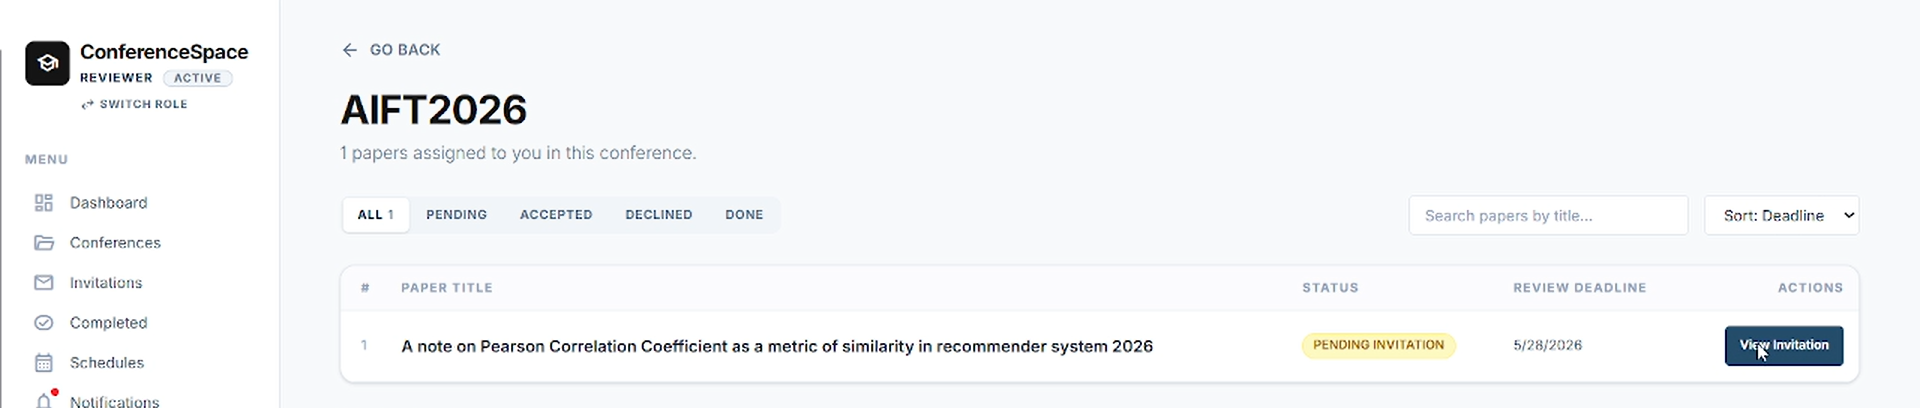
\includegraphics[width=0.95\textwidth]{images/chapter_3_uc04_reviewer_invitations_2.png}
  \end{tabular}
  \caption{Email thông báo lời mời (trên) và danh sách lời mời tham gia phản biện trong hệ thống (dưới)}
  \label{fig:uc04-invitations-cut}
\end{figure}

Hình~\ref{fig:uc04-invitations-cut} minh họa giao diện tiếp nhận thông báo và danh sách lời mời tham gia phản biện hội nghị.

\begin{figure}[H]
  \centering
  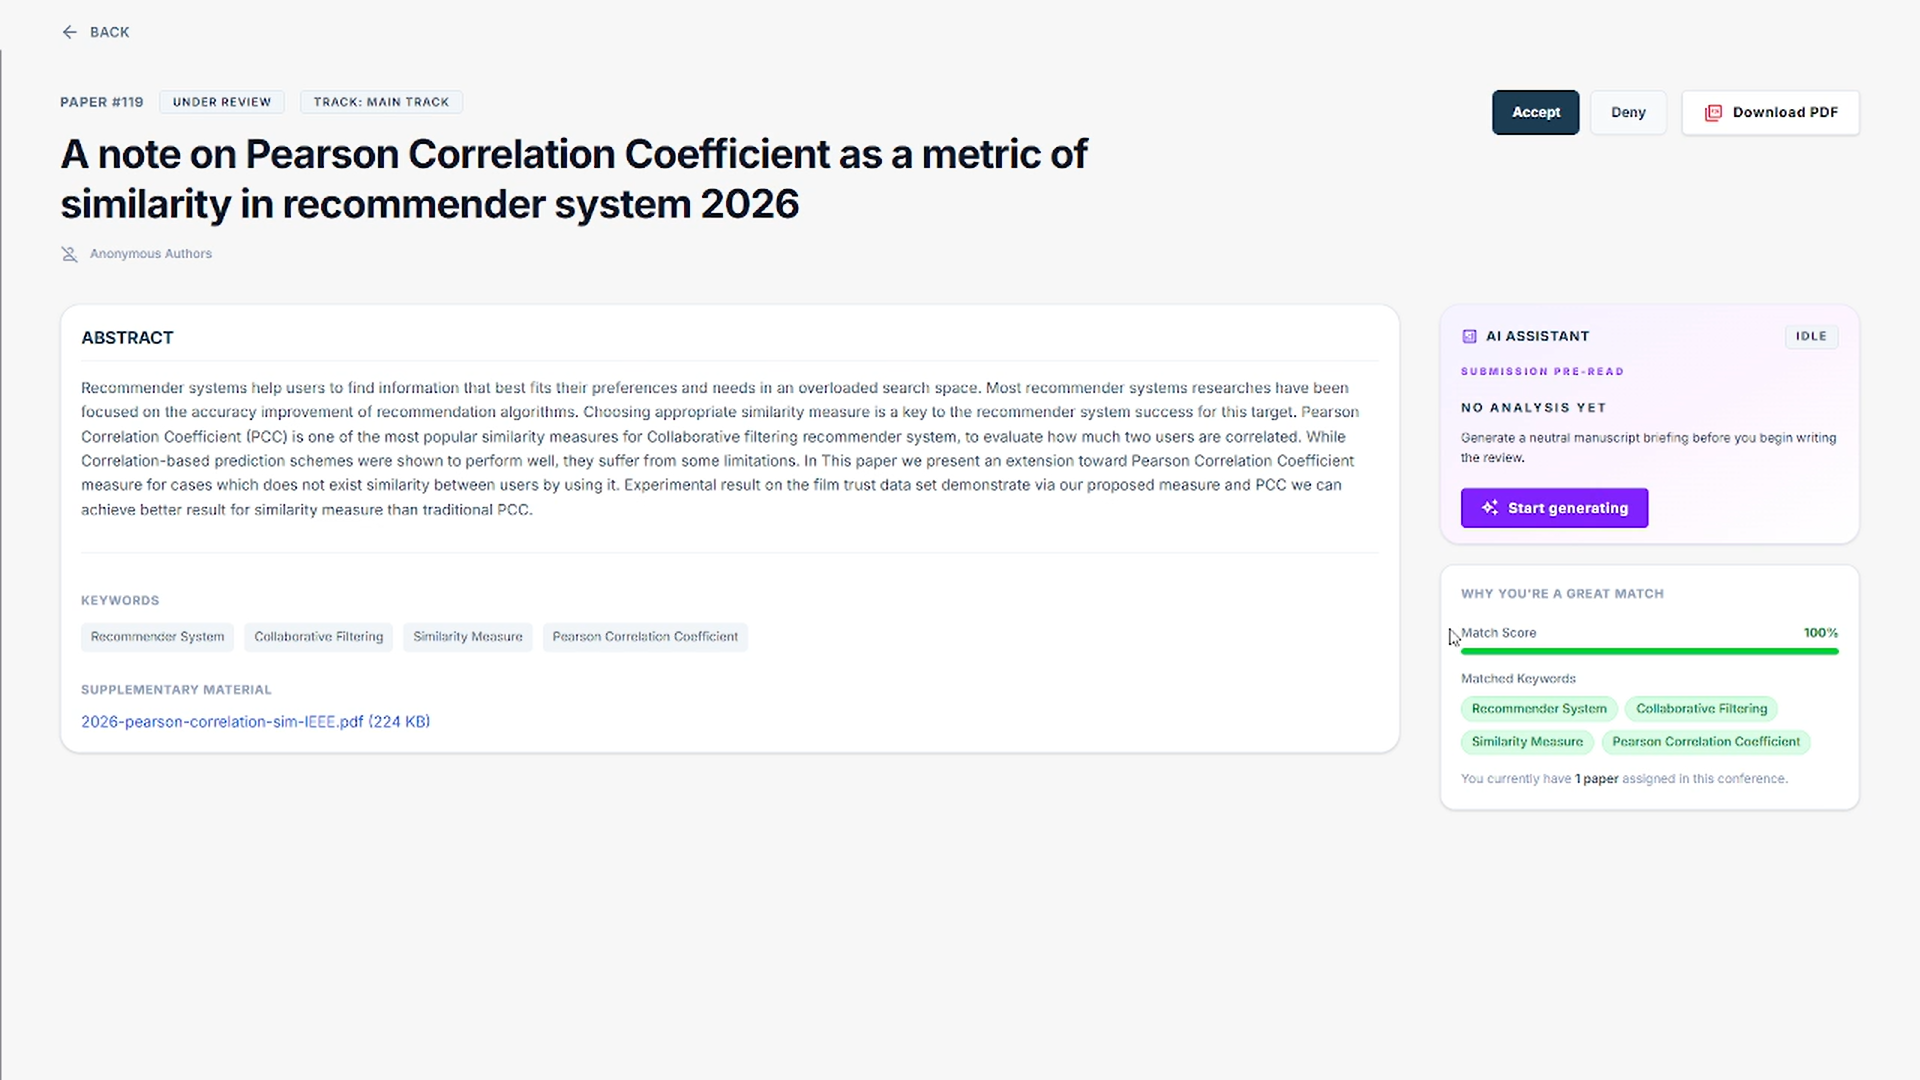
\includegraphics[width=0.95\textwidth]{images/chapter_3_uc04_accept_deny_assignment.png}
  \caption{Giao diện chi tiết bài nộp để Phản biện viên chấp nhận hoặc từ chối phân công}
  \label{fig:uc04-accept-deny-cut}
\end{figure}

Sau khi Chủ tọa tạo phân công, Phản biện viên dùng giao diện tại Hình~\ref{fig:uc04-accept-deny-cut} để xem bài nộp và chấp nhận hoặc từ chối phân công.

\subsubsection{UC-05. Đọc, soạn và gửi phản biện có AI hỗ trợ}

Phản biện viên mở bài được phân công, đọc bản thảo và nhập điểm, nhận xét, khuyến nghị cùng mức độ tự tin. Reviewer Initial Analysis có thể cung cấp bản định hướng ban đầu, nhưng Phản biện viên phải đối chiếu nội dung này với bài gốc và tự hình thành nhận định. Trước khi gửi, Review Quality Auditor rà soát mức độ đầy đủ, cụ thể và nhất quán của bản nháp. Phản biện viên xem các phát hiện, chỉnh sửa khi cần và xác nhận gửi phản biện.

\begin{figure}[H]
  \centering
  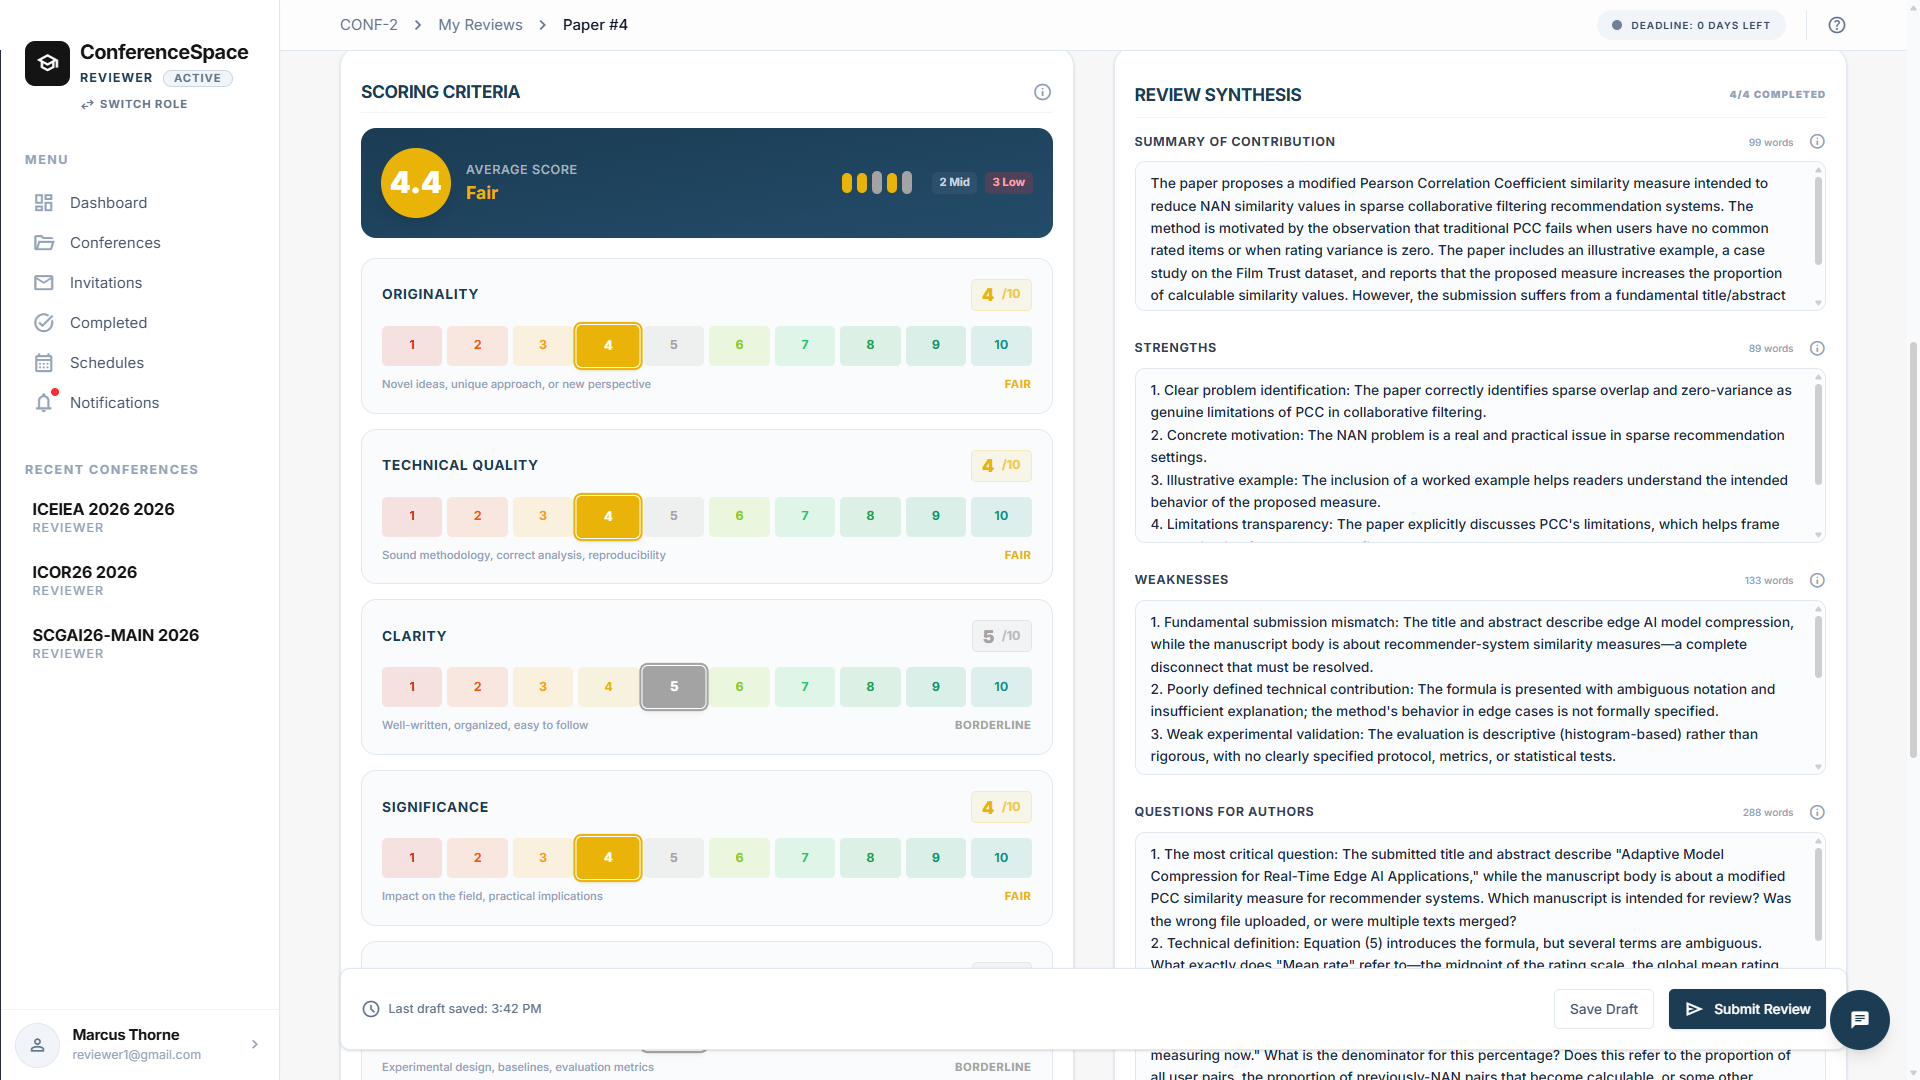
\includegraphics[width=0.95\textwidth]{images/chapter_3_uc05_reviewer_workspace_1.png}
  \caption{Không gian đọc bài và soạn phản biện của Phản biện viên}
  \label{fig:uc05-workspace-cut}
\end{figure}

Hình~\ref{fig:uc05-workspace-cut} đặt hai chức năng AI vào đúng bối cảnh sử dụng: chúng hỗ trợ một quy trình mà Phản biện viên vẫn phải đọc bản thảo, nhập nhận xét và chịu trách nhiệm về bản phản biện cuối cùng.

\begin{figure}[H]
  \centering
  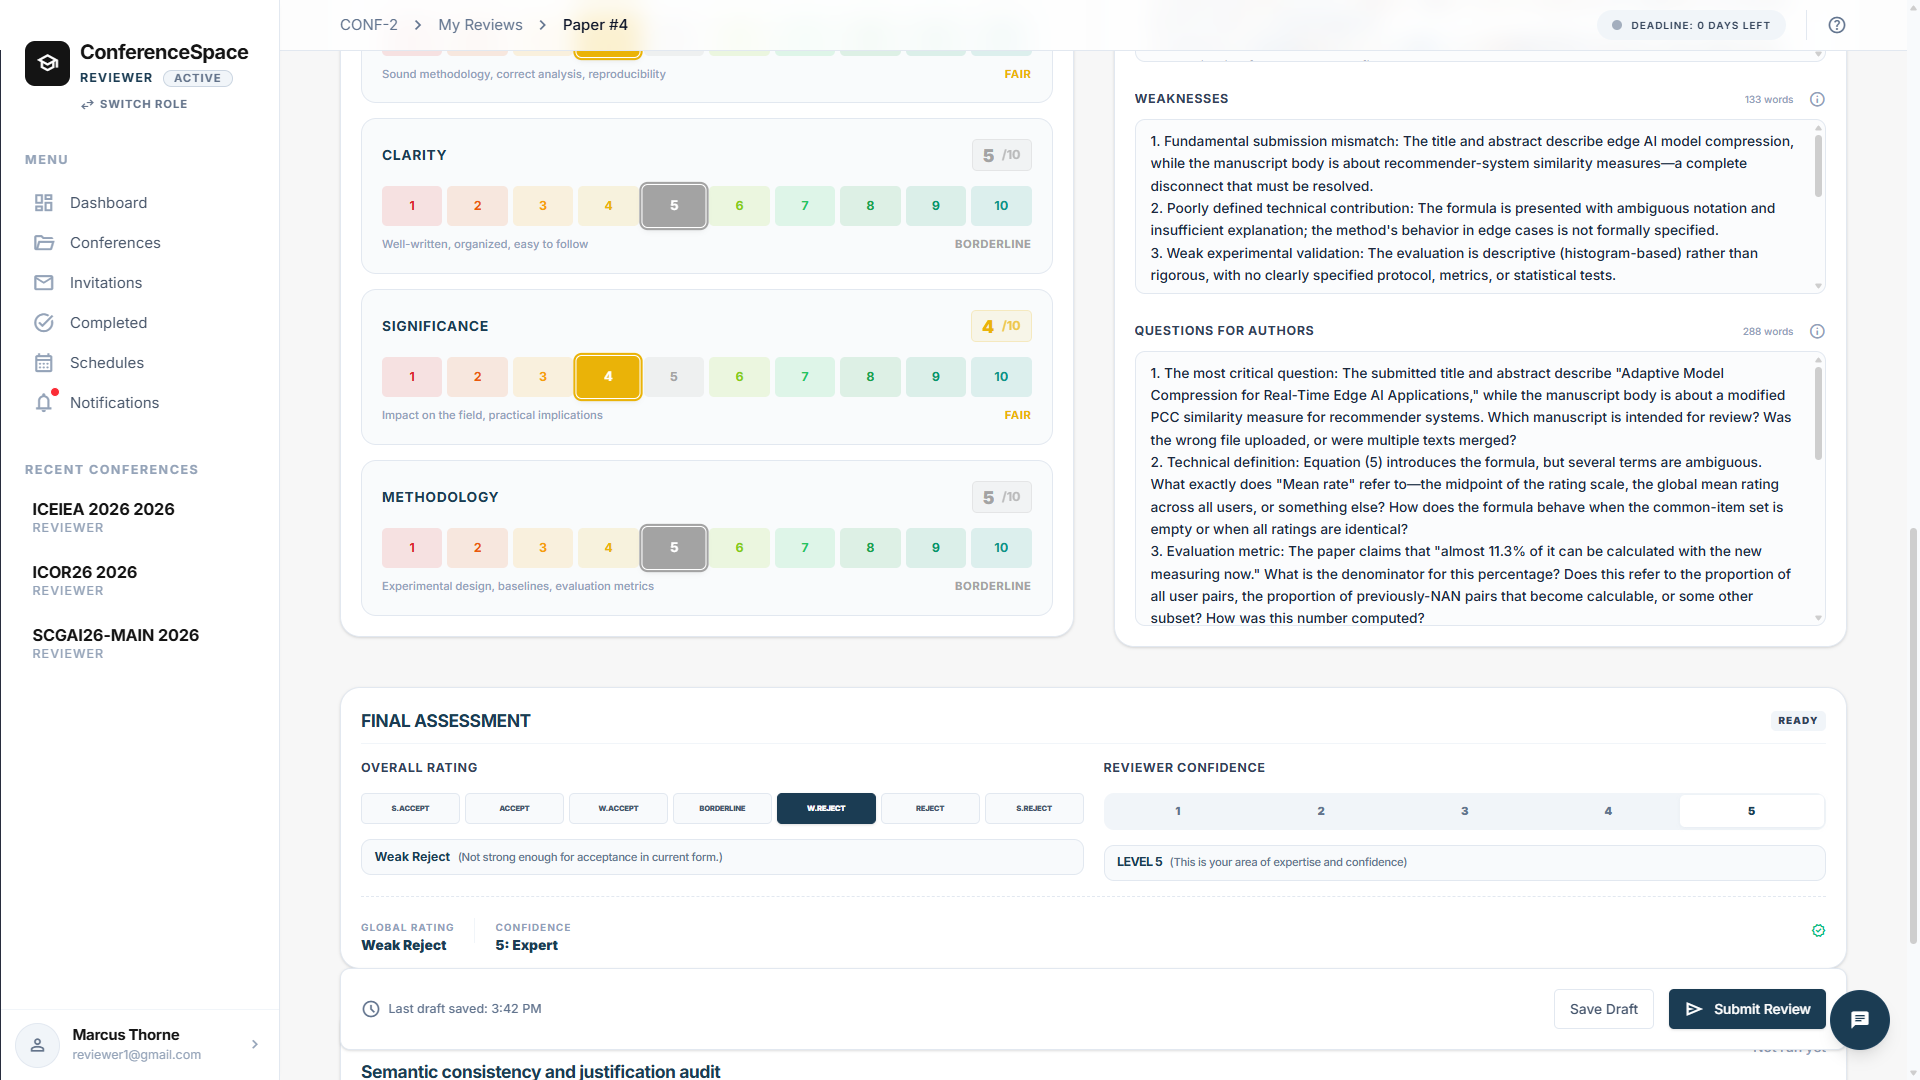
\includegraphics[width=0.95\textwidth]{images/chapter_3_uc05_reviewer_workspace_2.png}
  \caption{Không gian làm việc với biểu mẫu phản biện mở rộng của Phản biện viên}
  \label{fig:uc05-workspace-2-cut}
\end{figure}

Hình~\ref{fig:uc05-workspace-2-cut} trình bày một biến thể khác của không gian làm việc và biểu mẫu phản biện.

\begin{figure}[H]
  \centering
  \makebox[\textwidth][c]{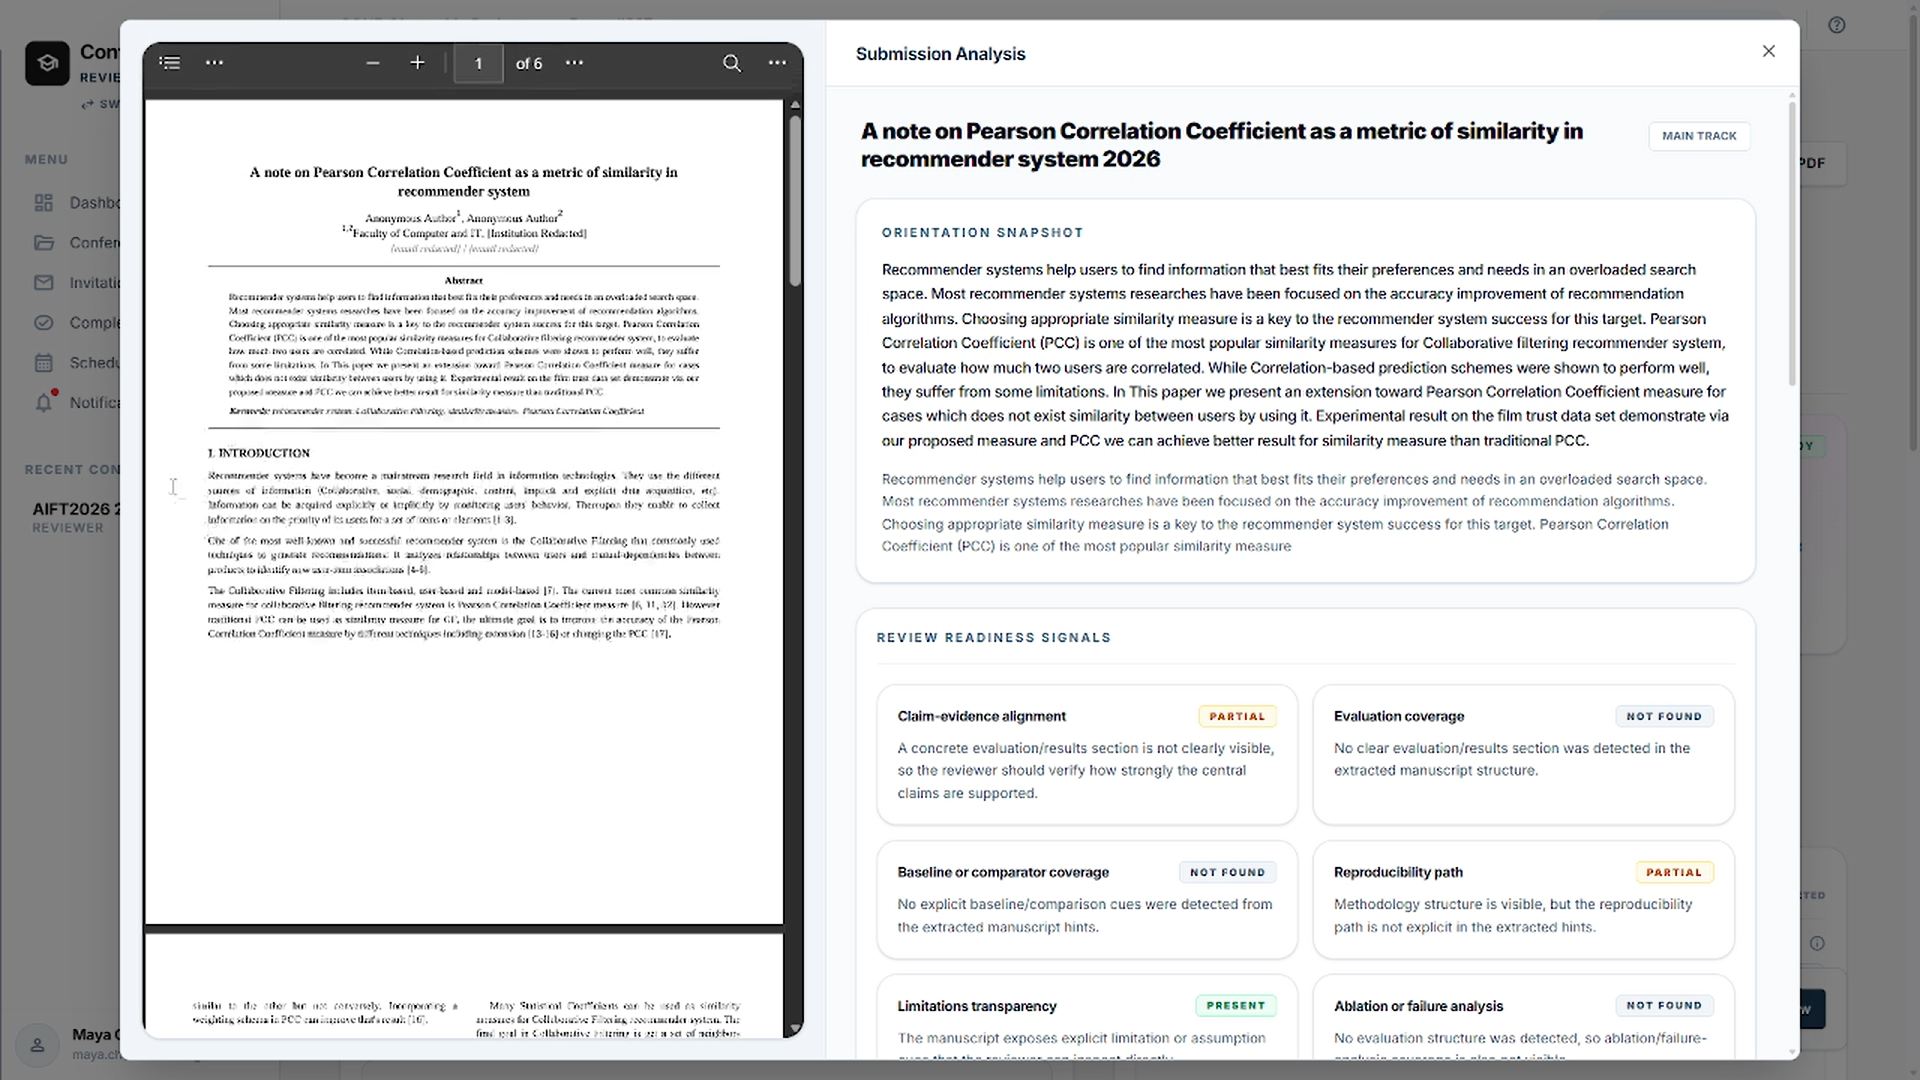
\includegraphics[width=1.10\textwidth]{images/chapter_3_uc05_reviewer_initial_analysis.png}}
  \caption{Bản định hướng đọc của Reviewer Initial Analysis}
  \label{fig:uc05-ria-cut}
\end{figure}

Hình~\ref{fig:uc05-ria-cut} thể hiện bản định hướng đọc do Reviewer Initial Analysis tạo ra để Phản biện viên tham khảo trước khi bắt đầu soạn phản biện.

\begin{figure}[H]
  \centering
  \makebox[\textwidth][c]{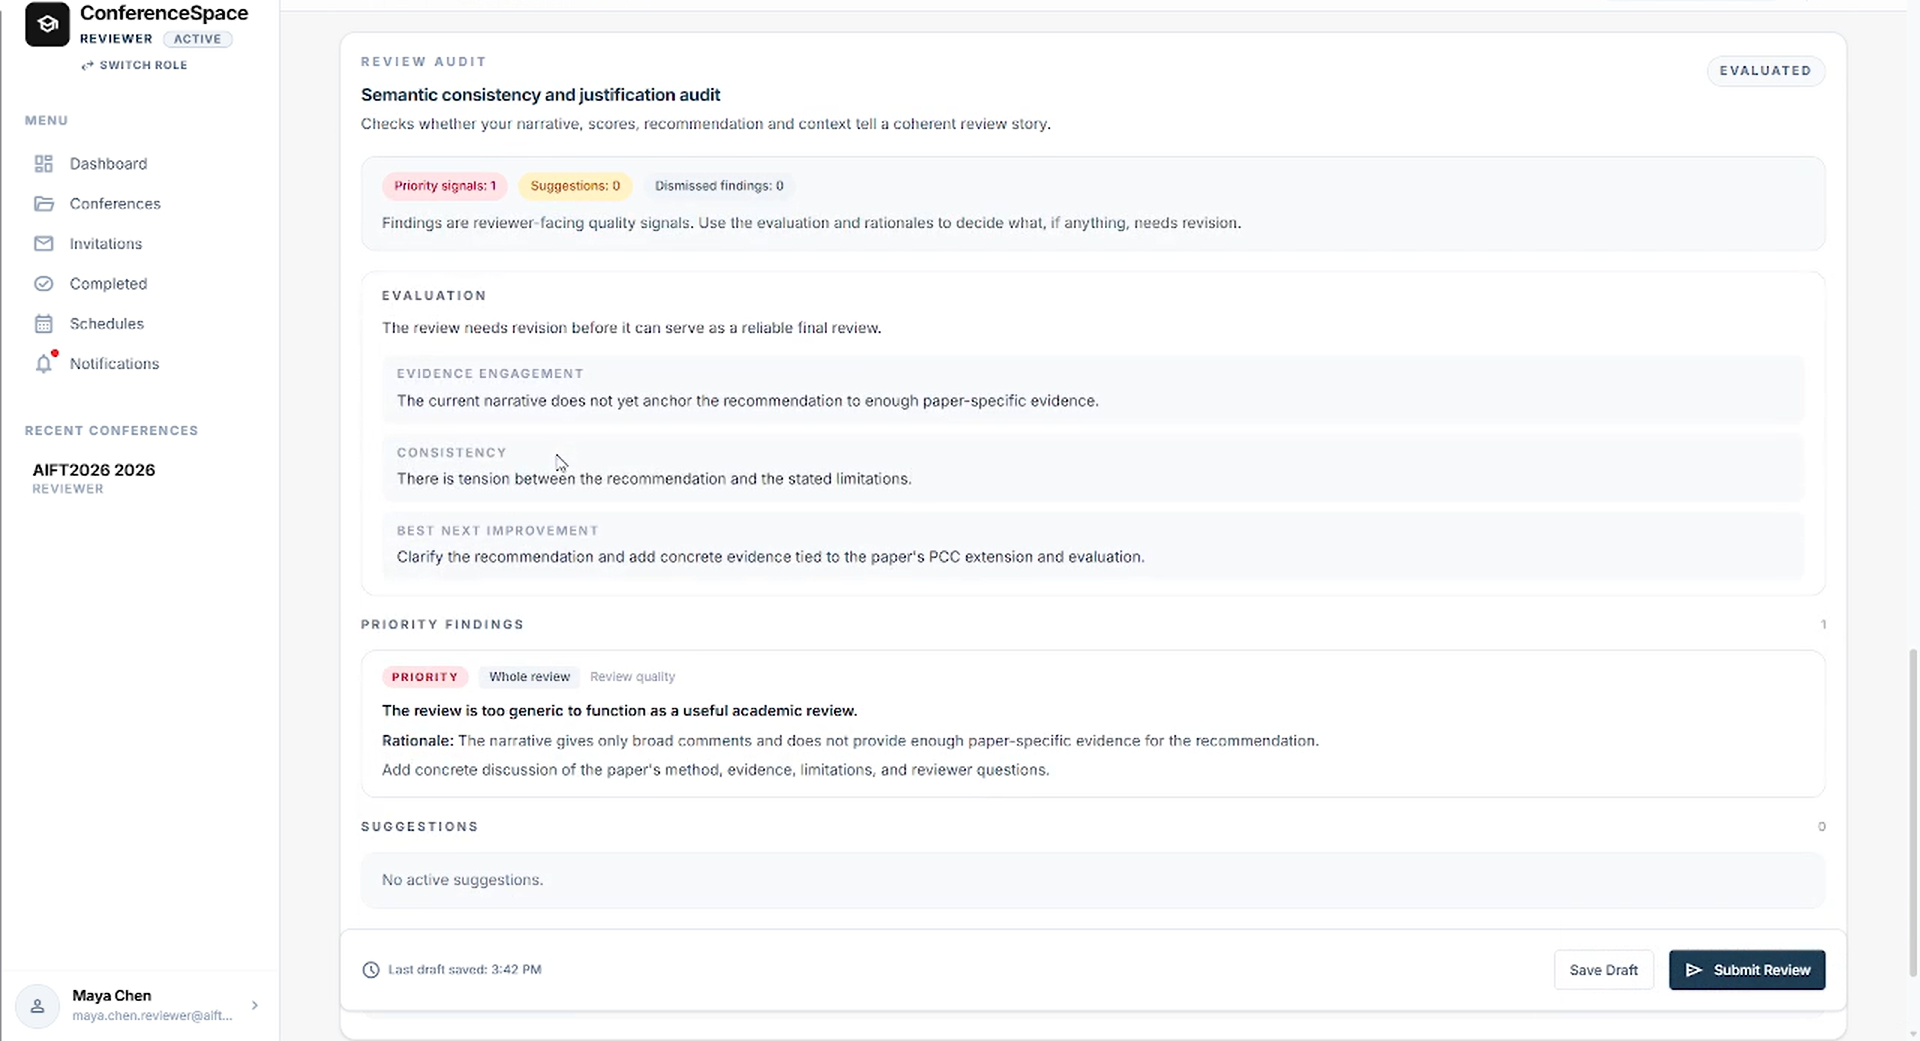
\includegraphics[width=1.10\textwidth]{images/chapter_3_uc05_reviewer_quality_auditor.png}}
  \caption{Bảng rà soát bản nháp của Review Quality Auditor}
  \label{fig:uc05-rqa-cut}
\end{figure}

Trước khi gửi phản biện, Phản biện viên xem bảng rà soát do Review Quality Auditor tạo ra tại Hình~\ref{fig:uc05-rqa-cut}.

Review Quality Auditor chạy trước khi gửi để đưa các phát hiện vào bảng rà soát. Phát hiện mức \textit{blocking} được làm nổi bật nhưng không ngăn Phản biện viên gửi phản biện. Nếu tác vụ rà soát không thể hoàn tất do lỗi dịch vụ, backend yêu cầu Phản biện viên xác nhận tiếp tục mà không có kết quả rà soát và ghi sự kiện này vào nhật ký. Hệ thống phân biệt phát hiện về chất lượng với lỗi không thể thực hiện bước rà soát: phát hiện chất lượng cung cấp thông tin để Phản biện viên xem xét, còn lỗi thực thi được thông báo rõ và ghi vào nhật ký.

\subsubsection{UC-06. Phân công phản biện có kiểm tra xung đột lợi ích}

Hệ thống chuẩn bị các cặp bài nộp--Phản biện viên, tính điểm phù hợp, loại các cặp có xung đột lợi ích khỏi đề xuất tự động và theo dõi số phân công được tạo trong cùng lượt chạy. Trước khi điều chỉnh hoặc xác nhận, Chủ tọa xem điểm số, lý do đối sánh, trạng thái kiểm tra xung đột lợi ích, tải phát sinh trong lượt chạy và danh sách bài chưa đủ Phản biện viên. Phản hồi \CodeBreak{AutoAssignResponse} không liệt kê đầy đủ từng cặp ứng viên bị loại. Khi Chủ tọa thêm đề xuất thủ công, backend kiểm tra quyền và trả cảnh báo xung đột lợi ích nhưng hiện chưa ngăn lưu; vì vậy, Chủ tọa phải xử lý cảnh báo trước khi xác nhận phương án.

\begin{figure}[H]
  \centering
  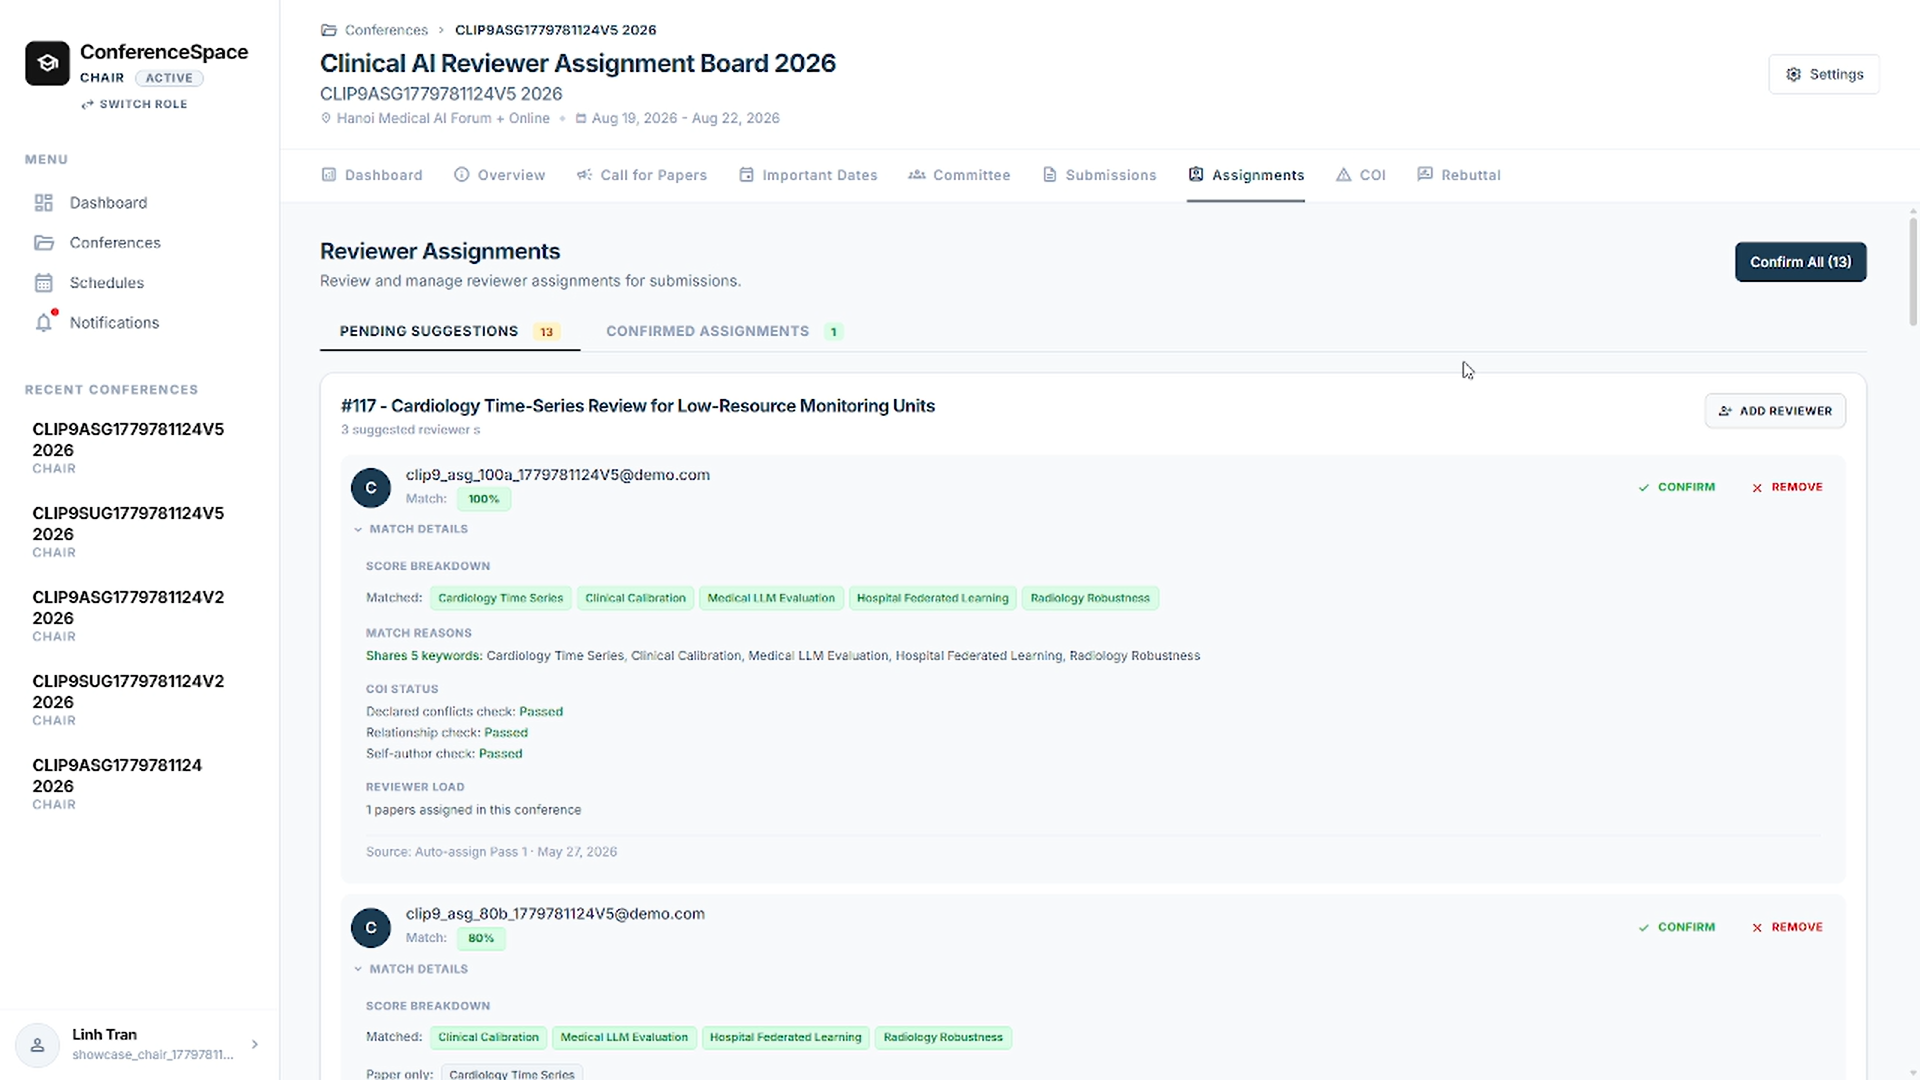
\includegraphics[width=0.95\textwidth]{images/chapter_3_uc06_assignment_dashboard.png}
  \caption{Giao diện bảng điều khiển quản lý phân công phản biện của Chủ tọa}
  \label{fig:uc06-dashboard-cut}
\end{figure}

Hình~\ref{fig:uc06-dashboard-cut} minh họa bảng điều khiển quản lý phân công phản biện của Chủ tọa.

\begin{figure}[H]
  \centering
  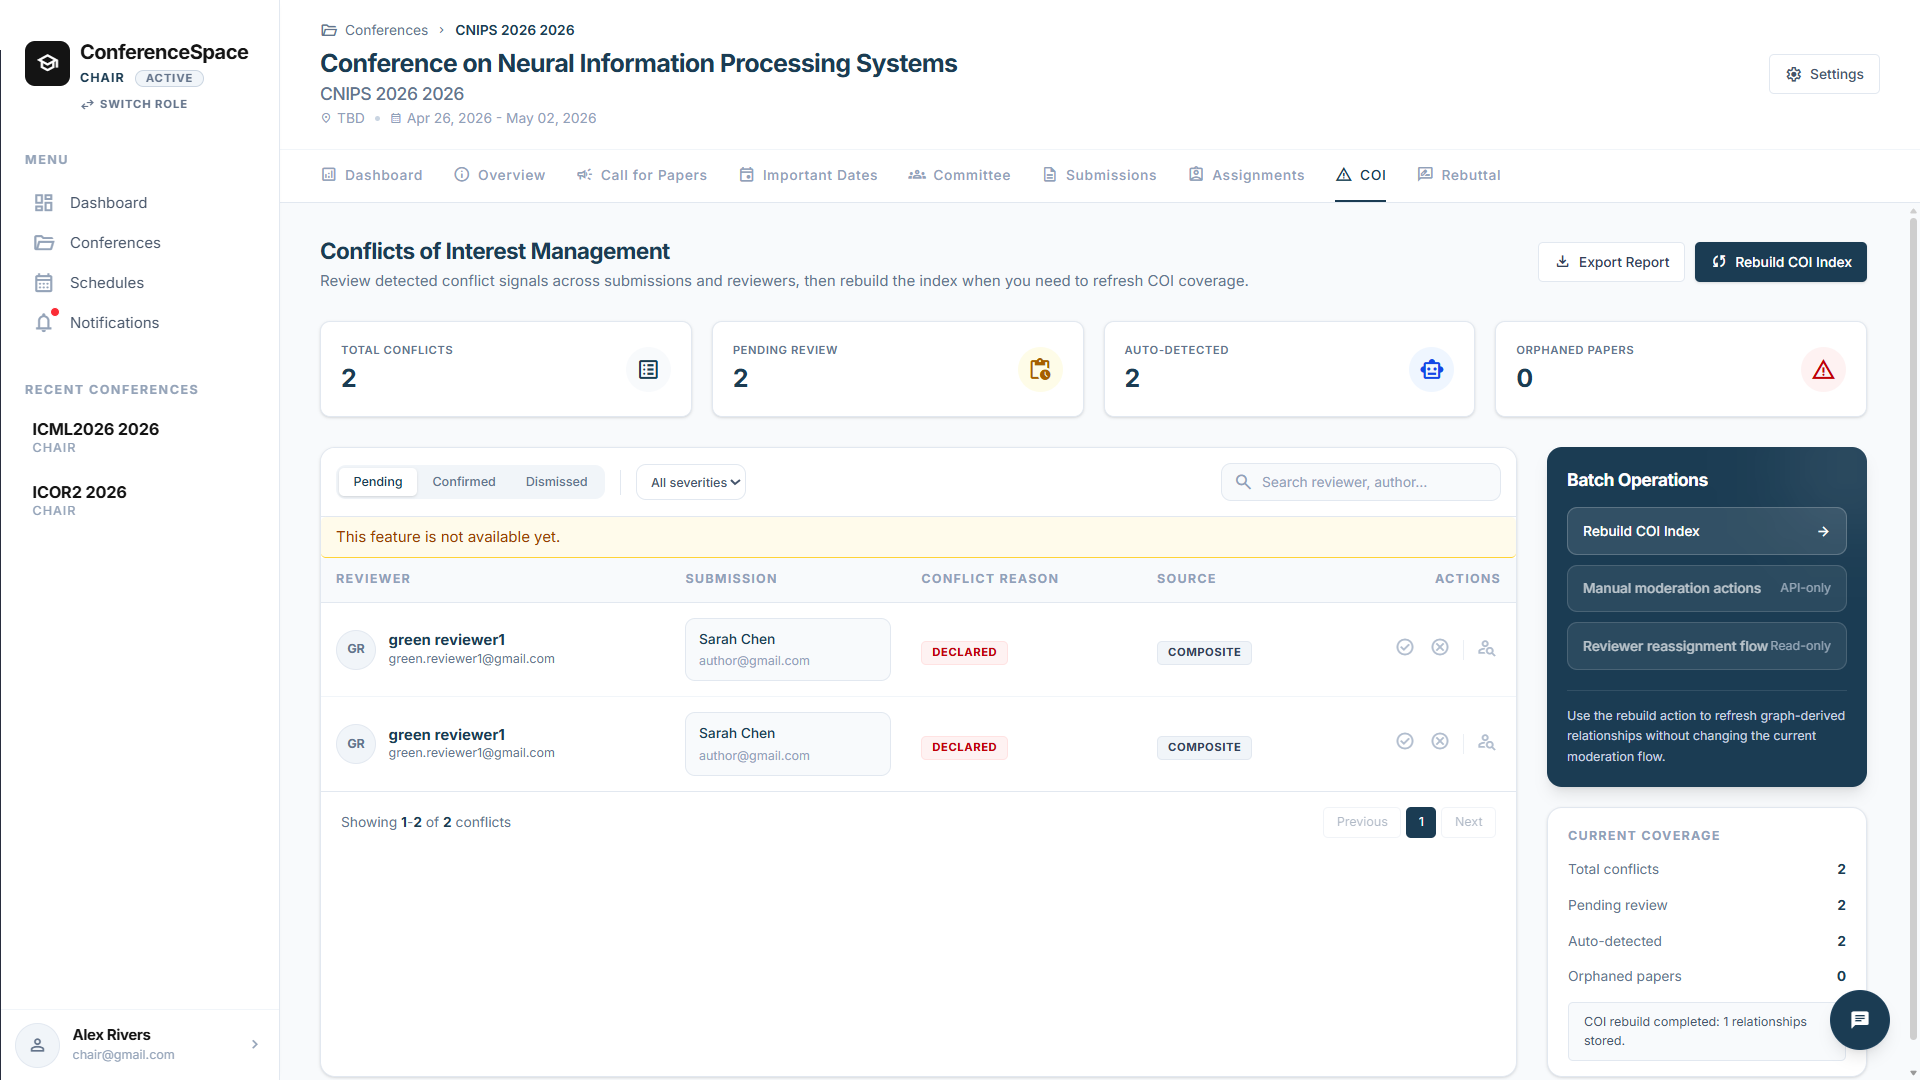
\includegraphics[width=0.95\textwidth]{images/chapter_3_uc06_coi_verification.png}
  \caption{Giao diện kiểm tra xung đột lợi ích giữa phản biện viên và bài nộp}
  \label{fig:uc06-coi-verification-cut}
\end{figure}

Hình~\ref{fig:uc06-coi-verification-cut} minh họa giao diện kiểm tra xung đột lợi ích giữa phản biện viên và bài nộp.

\begin{figure}[H]
  \centering
  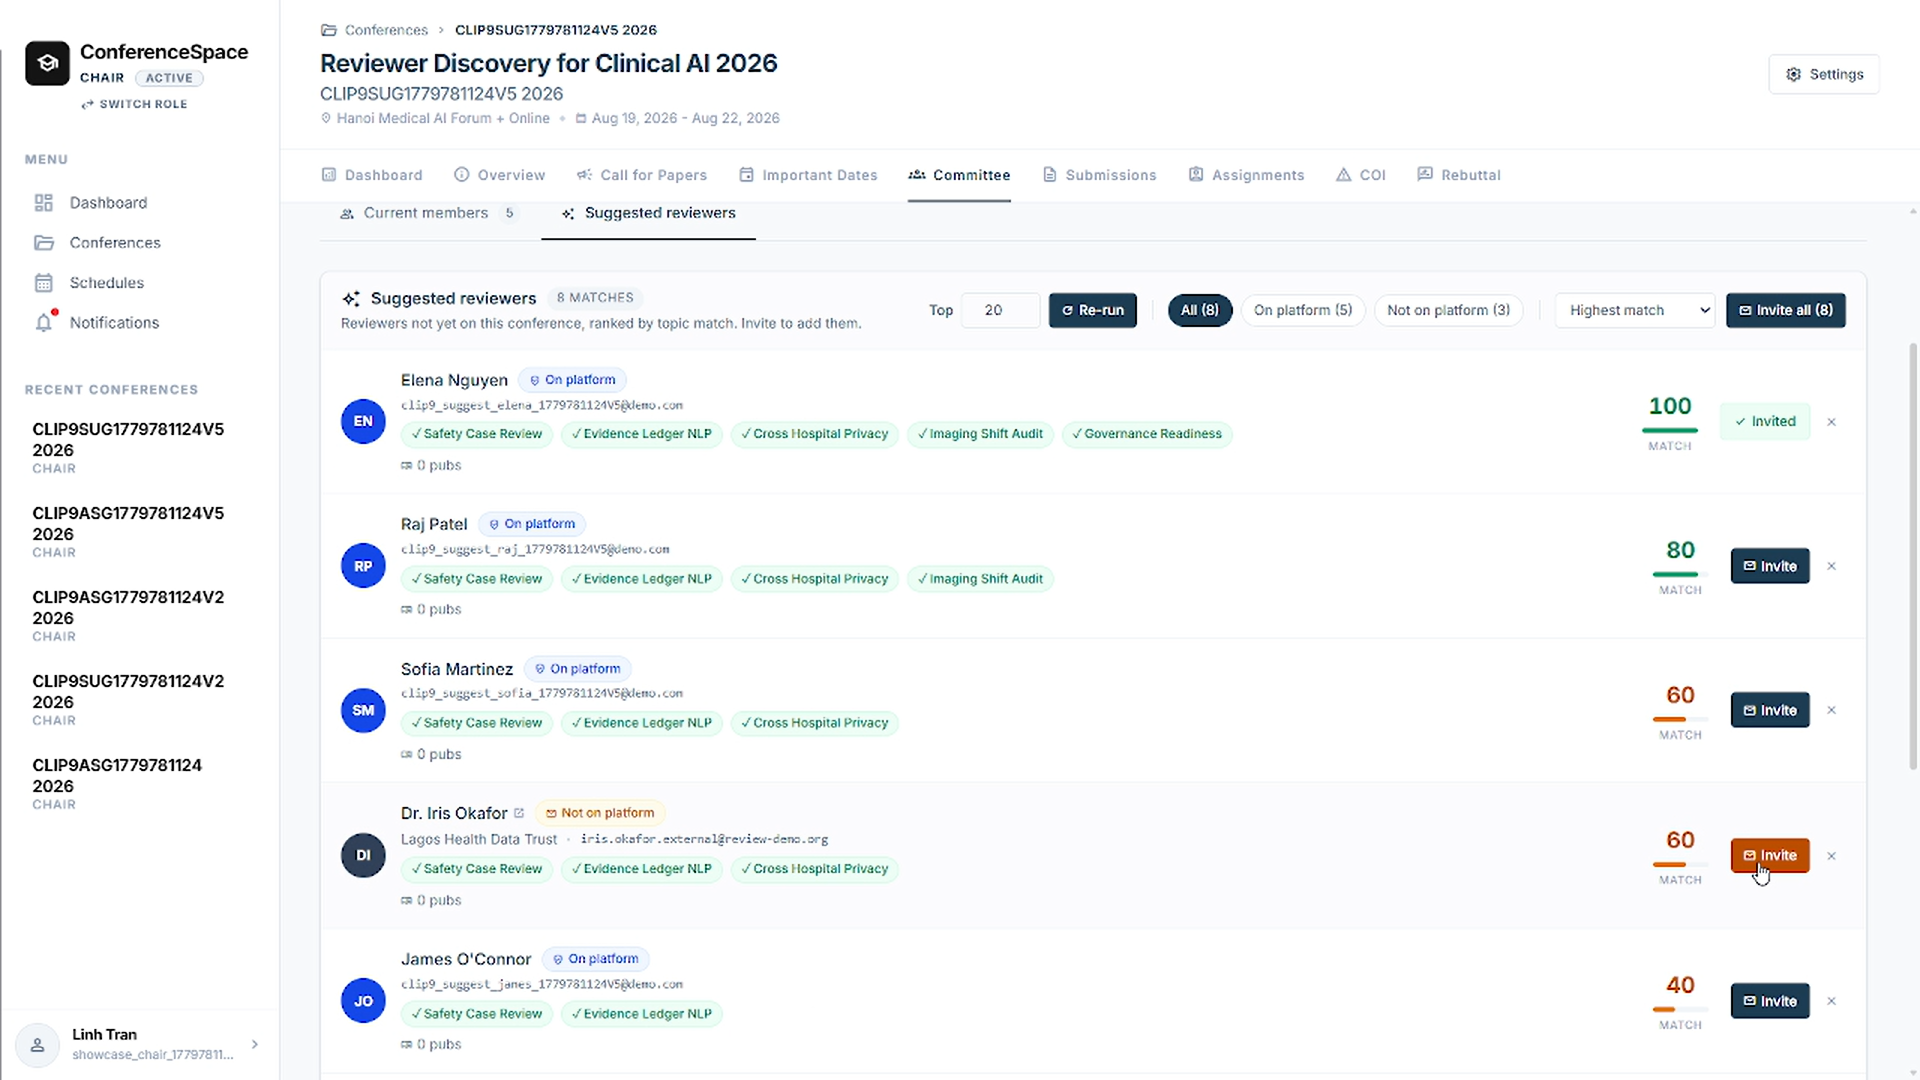
\includegraphics[width=0.95\textwidth]{images/chapter_3_uc06_assignment_suggestions.png}
  \caption{Danh sách đề xuất đối sánh và điểm phù hợp để Chủ tọa xem xét}
  \label{fig:uc06-suggestions-cut}
\end{figure}

Hình~\ref{fig:uc06-suggestions-cut} liệt kê các đề xuất đối sánh cùng điểm phù hợp để Chủ tọa xem xét trước khi xác nhận.

Công thức tính điểm, thủ tục phân công, lượt dự phòng và các trường hợp ngoại lệ được trình bày tại Mục~\ref{subsec:ch3-matching-cut}. Thuật toán tự động không nới ràng buộc xung đột lợi ích, kể cả khi hệ thống không tìm được đủ Phản biện viên; luồng thêm đề xuất thủ công hiện dùng cảnh báo thay cho cưỡng chế tại thời điểm ghi dữ liệu.

\subsubsection{UC-07. Quản lý hội nghị và theo dõi tiến độ}

Chủ tọa cấu hình thông tin hội nghị, chuyên đề, hạn chót nộp bài, biểu mẫu phản biện và chính sách; mời thành viên hội đồng chương trình; theo dõi số bài, tiến độ phản biện và các trường hợp cần xử lý. Hệ thống từ chối cấu hình thiếu trường bắt buộc, hạn chót nộp bài không hợp lệ hoặc thao tác của người dùng không có quyền. Bảng điều khiển hỗ trợ nhận biết các trường hợp cần xử lý nhưng không tự chuyển giai đoạn hoặc ra quyết định thay Chủ tọa.

\begin{figure}[H]
  \centering
  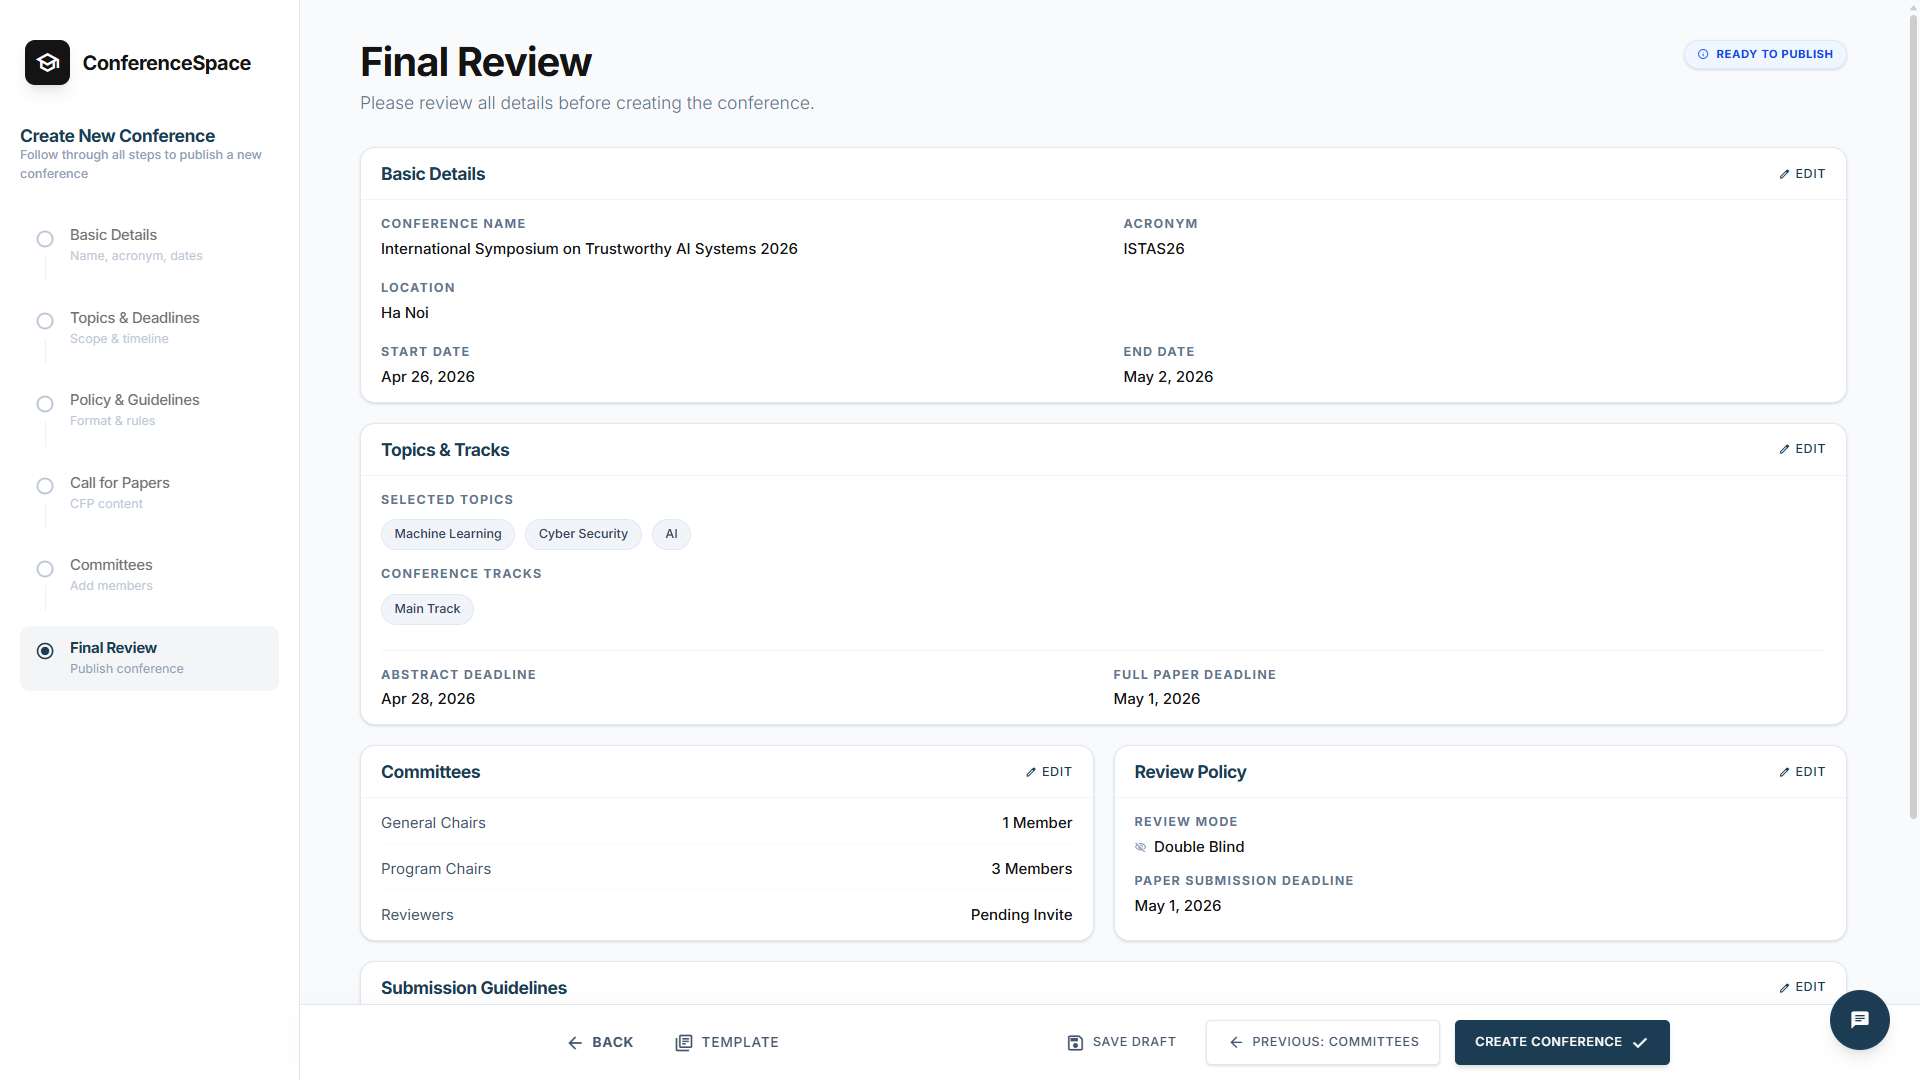
\includegraphics[width=0.95\textwidth]{images/chapter_3_uc07_conference_config.png}
  \caption{Giao diện thiết lập cấu hình thông tin và hạn chót nộp bài hội nghị của Chủ tọa}
  \label{fig:uc07-config-cut}
\end{figure}

Hình~\ref{fig:uc07-config-cut} thể hiện giao diện thiết lập cấu hình thông tin và hạn chót nộp bài hội nghị.

\begin{figure}[H]
  \centering
  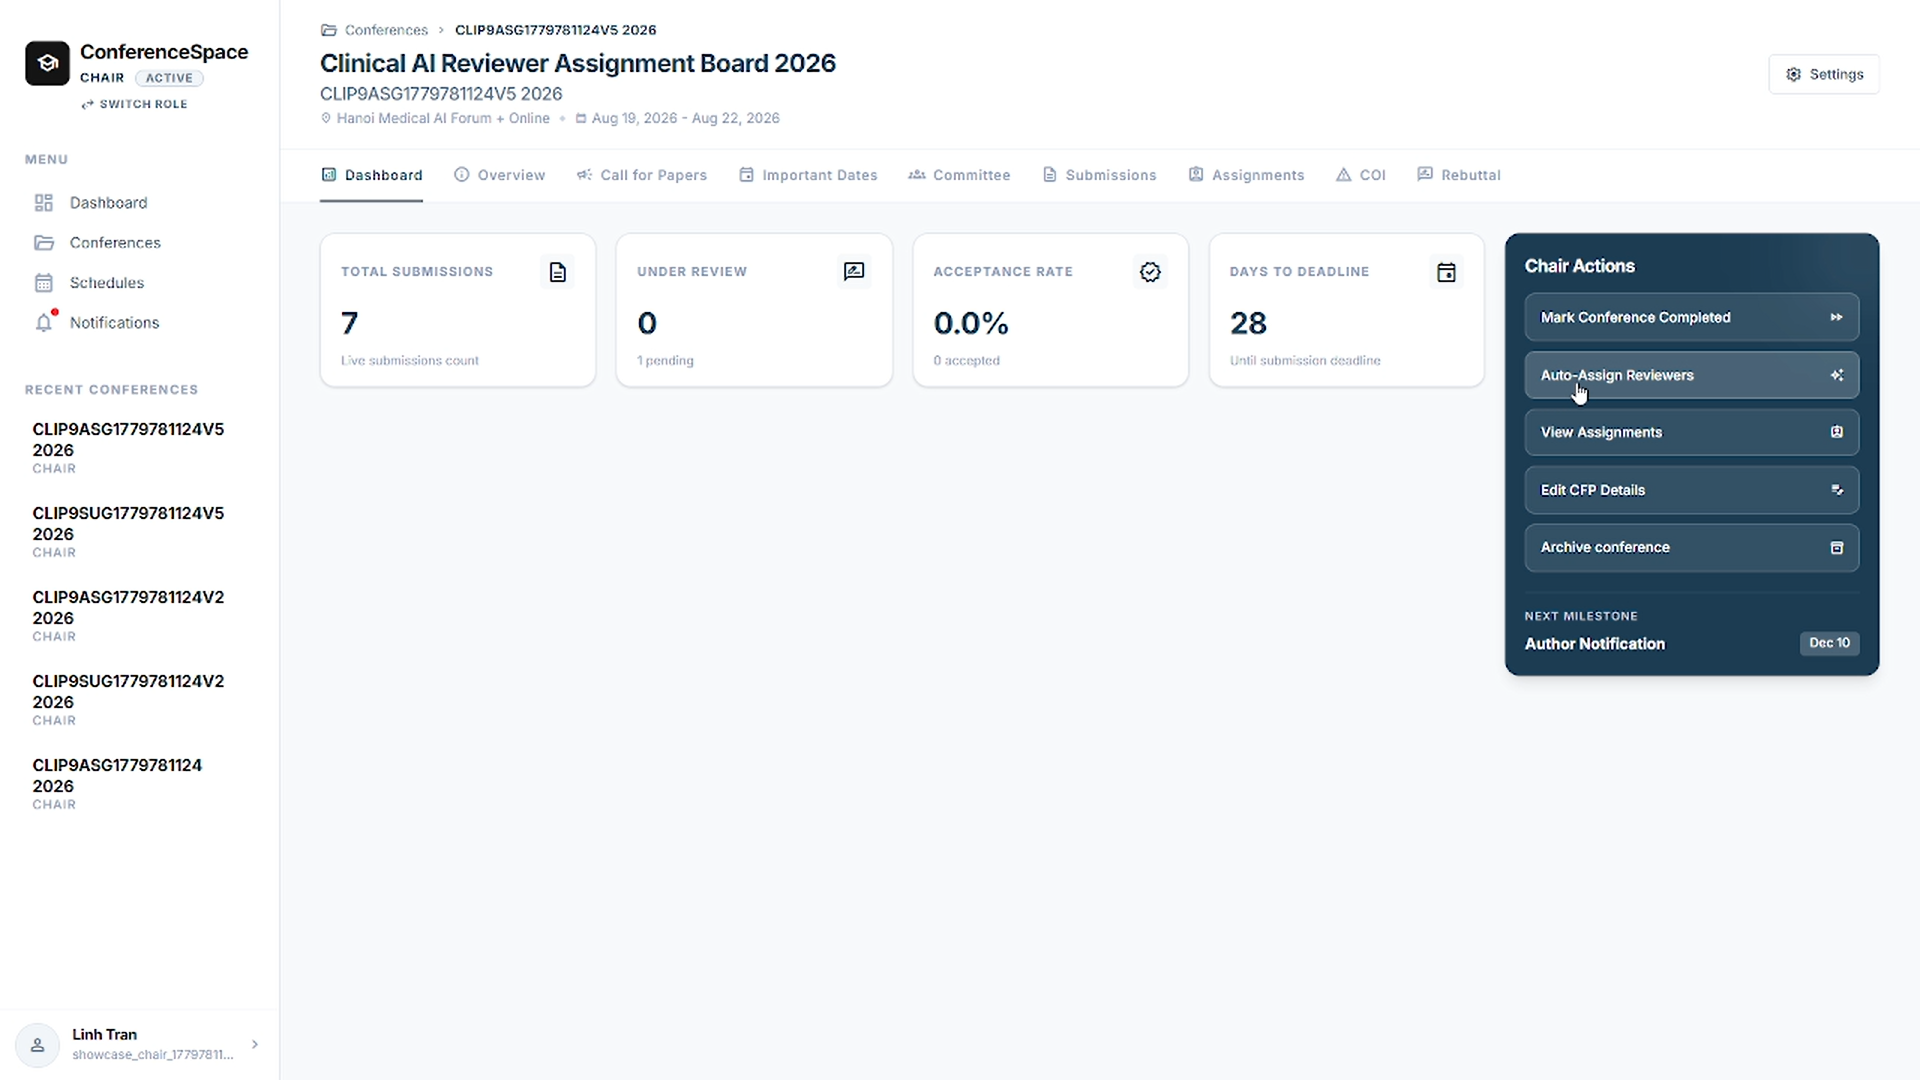
\includegraphics[width=0.95\textwidth]{images/chapter_3_uc07_chair_dashboard.png}
  \caption{Bảng điều khiển tiến độ hội nghị của Chủ tọa}
  \label{fig:uc07-dashboard-cut}
\end{figure}

Hình~\ref{fig:uc07-dashboard-cut} cung cấp cái nhìn tổng quan về hoạt động điều phối, bổ sung cho các hình chuyên biệt về đối sánh và hỗ trợ quyết định.

\begin{figure}[H]
  \centering
  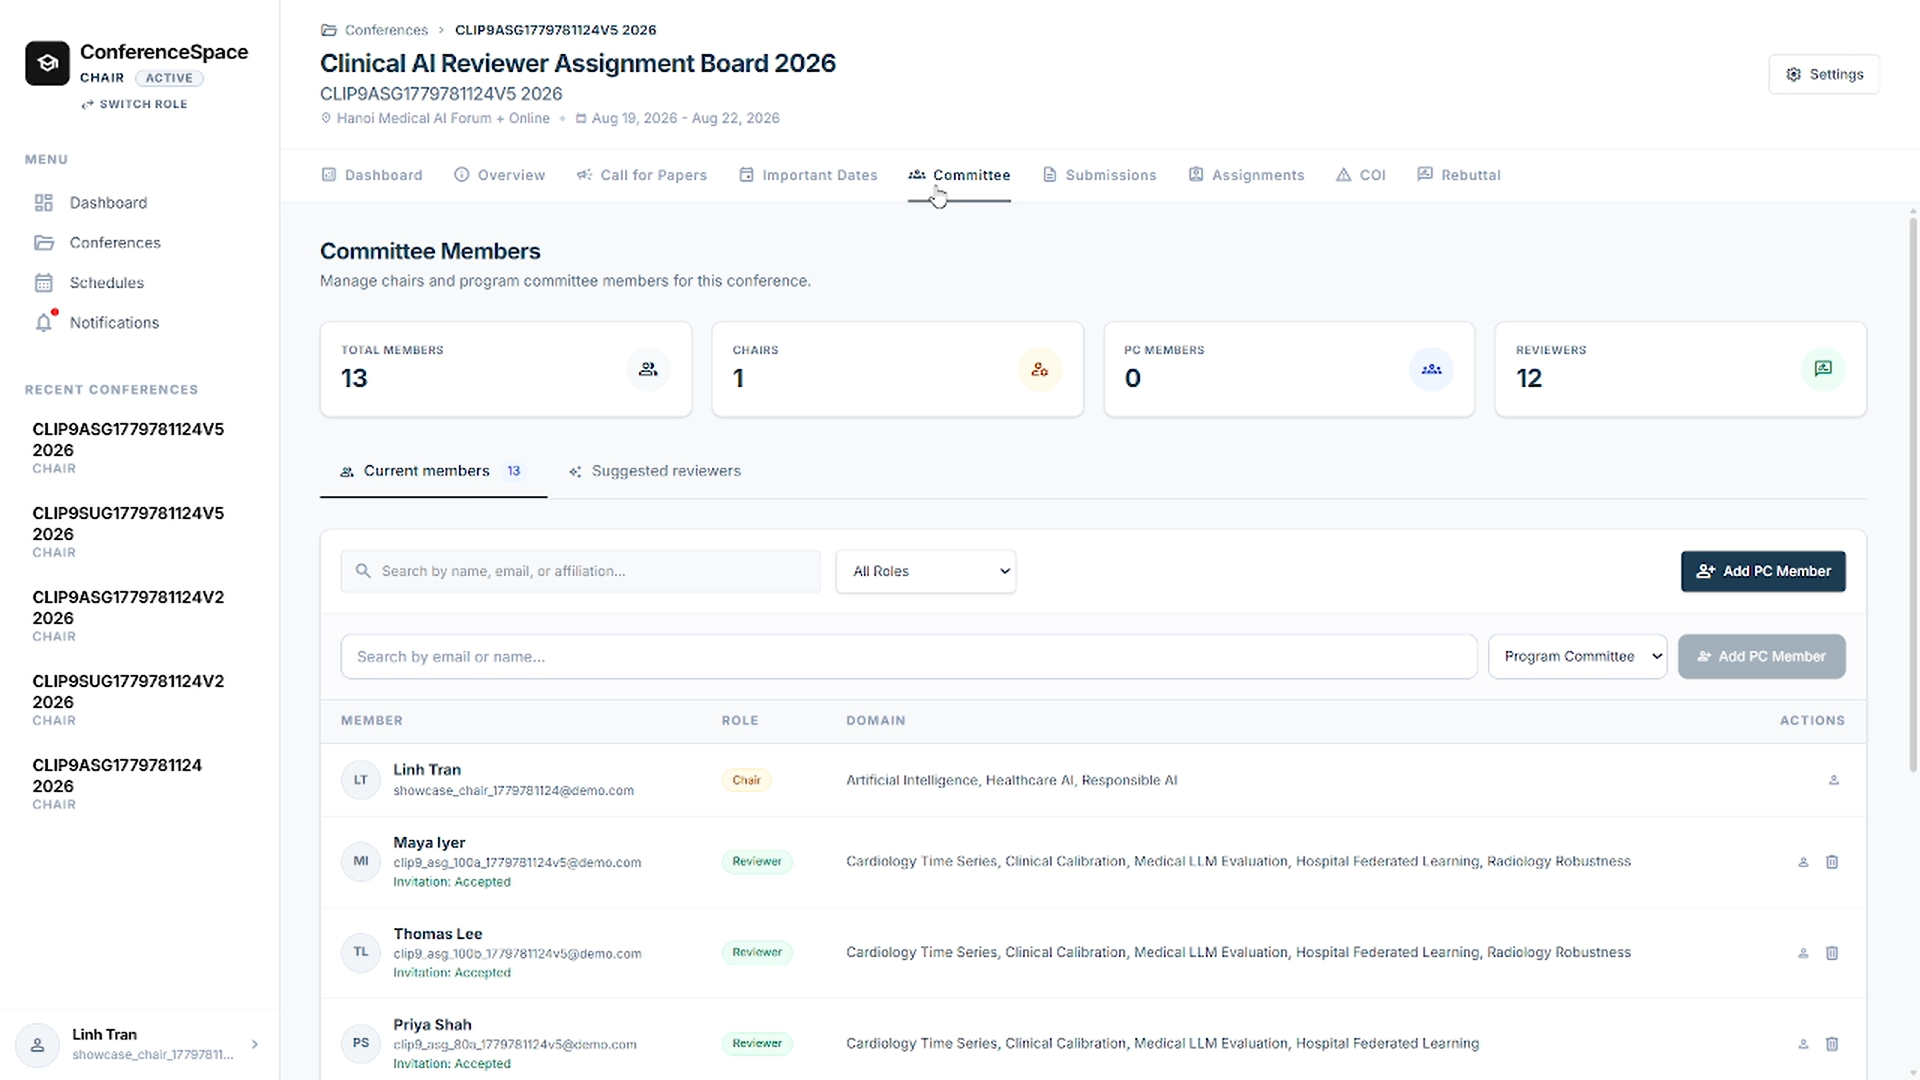
\includegraphics[width=0.95\textwidth]{images/chapter_3_uc07_committee_management.png}
  \caption{Giao diện quản lý ban chương trình và trạng thái lời mời phản biện viên}
  \label{fig:uc07-committee-cut}
\end{figure}

Hình~\ref{fig:uc07-committee-cut} minh họa giao diện quản lý ban chương trình và trạng thái lời mời phản biện viên.

\subsubsection{UC-08. Trao đổi theo bài nộp}

Chủ tọa hoặc Đồng chủ tọa mở giai đoạn phản hồi và kết thúc giai đoạn này trước khi ra quyết định; giai đoạn thảo luận chỉ được mở khi cấu hình hội nghị cho phép. Phản biện viên được phân công có thể tạo chuỗi thảo luận. Tác giả của bài và Phản biện viên trao đổi trong chuỗi tương ứng, còn Chủ tọa xem toàn bộ lịch sử ở chế độ giám sát. Sau khi đọc phản hồi, Phản biện viên có thể cập nhật điểm, khuyến nghị và nhận xét của bài mình phụ trách. Backend kiểm tra quan hệ giữa người dùng, bài nộp và chuỗi thảo luận trước mỗi thao tác. Nội dung trao đổi cùng đánh giá cập nhật được lưu với bài nộp và trở thành nguồn bằng chứng cho Chair Decision Copilot.

\begin{figure}[H]
  \centering
  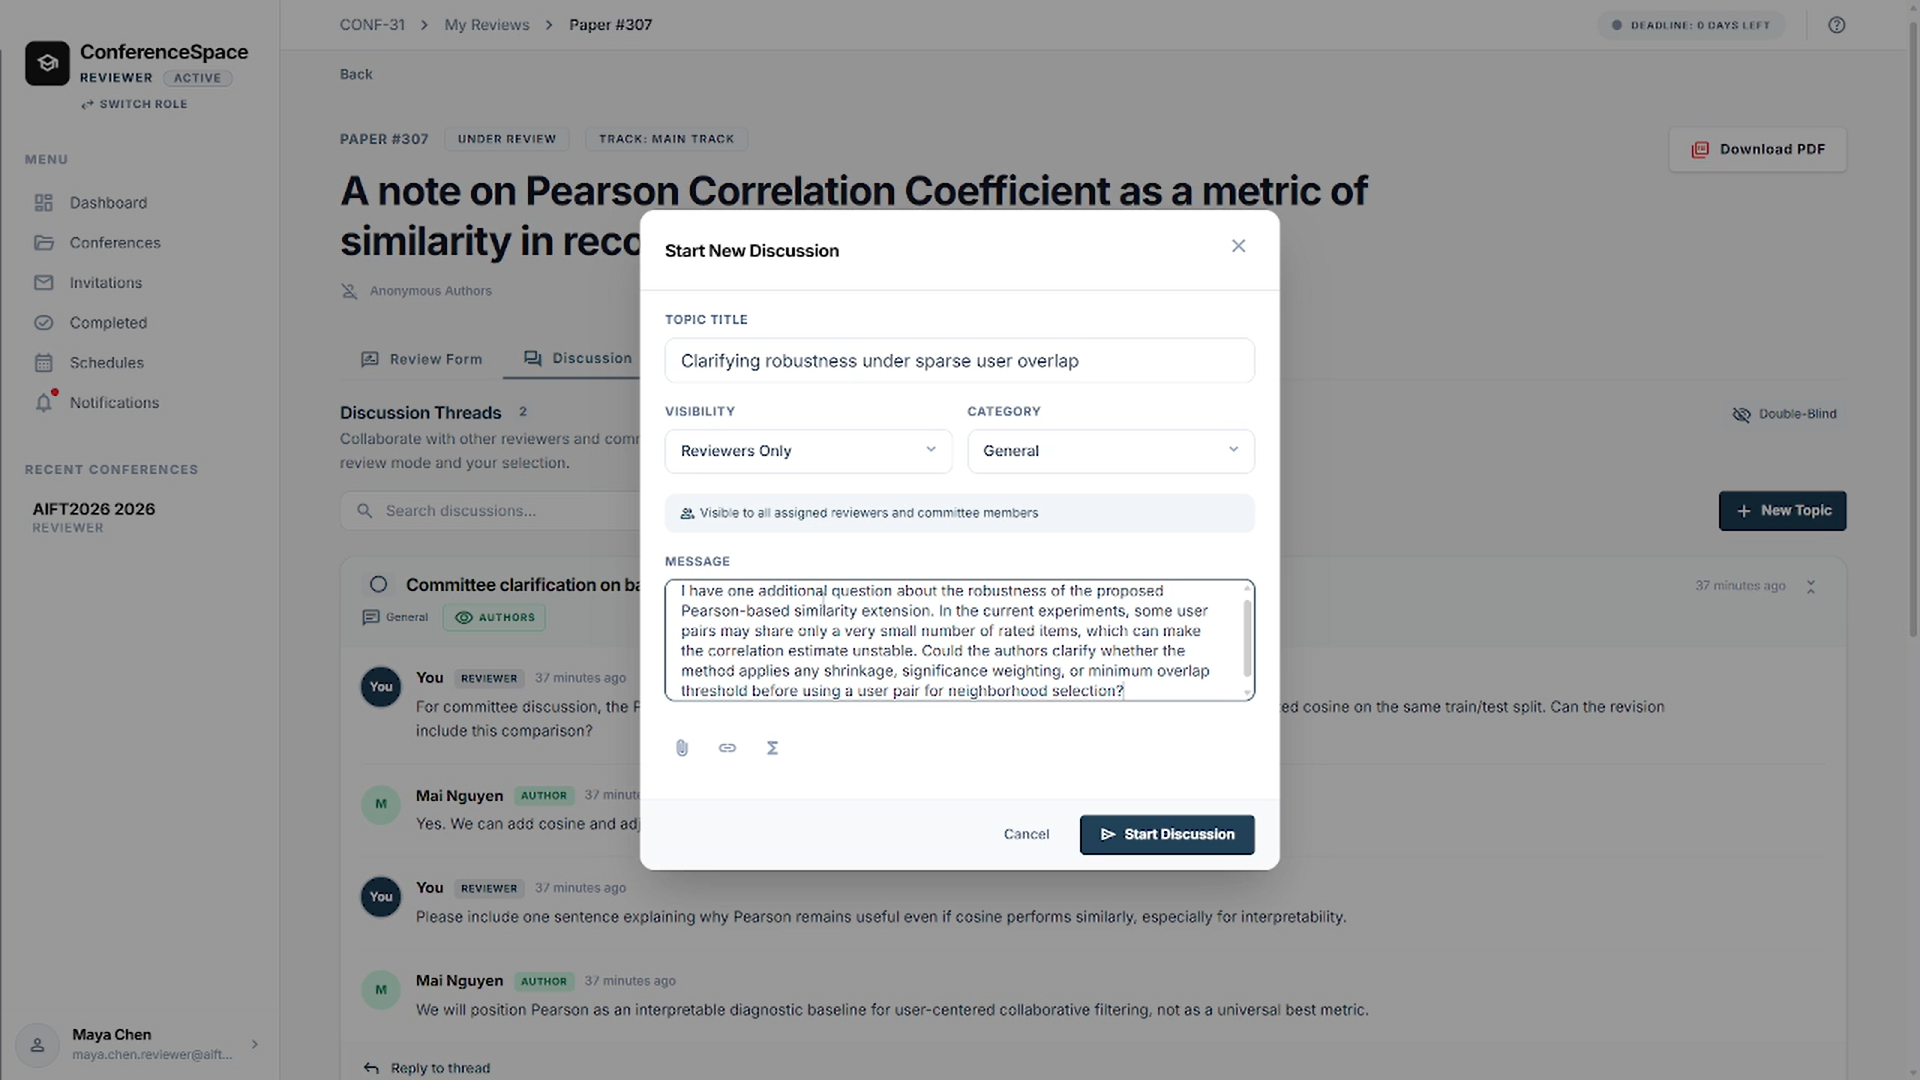
\includegraphics[width=0.95\textwidth]{images/chapter_3_uc08_create_discussion.png}
  \caption{Giao diện khởi tạo chủ đề thảo luận mới cho bài nộp}
  \label{fig:uc08-create-discussion-cut}
\end{figure}

Hình~\ref{fig:uc08-create-discussion-cut} minh họa giao diện khởi tạo chủ đề thảo luận mới cho bài nộp.

\begin{figure}[H]
  \centering
  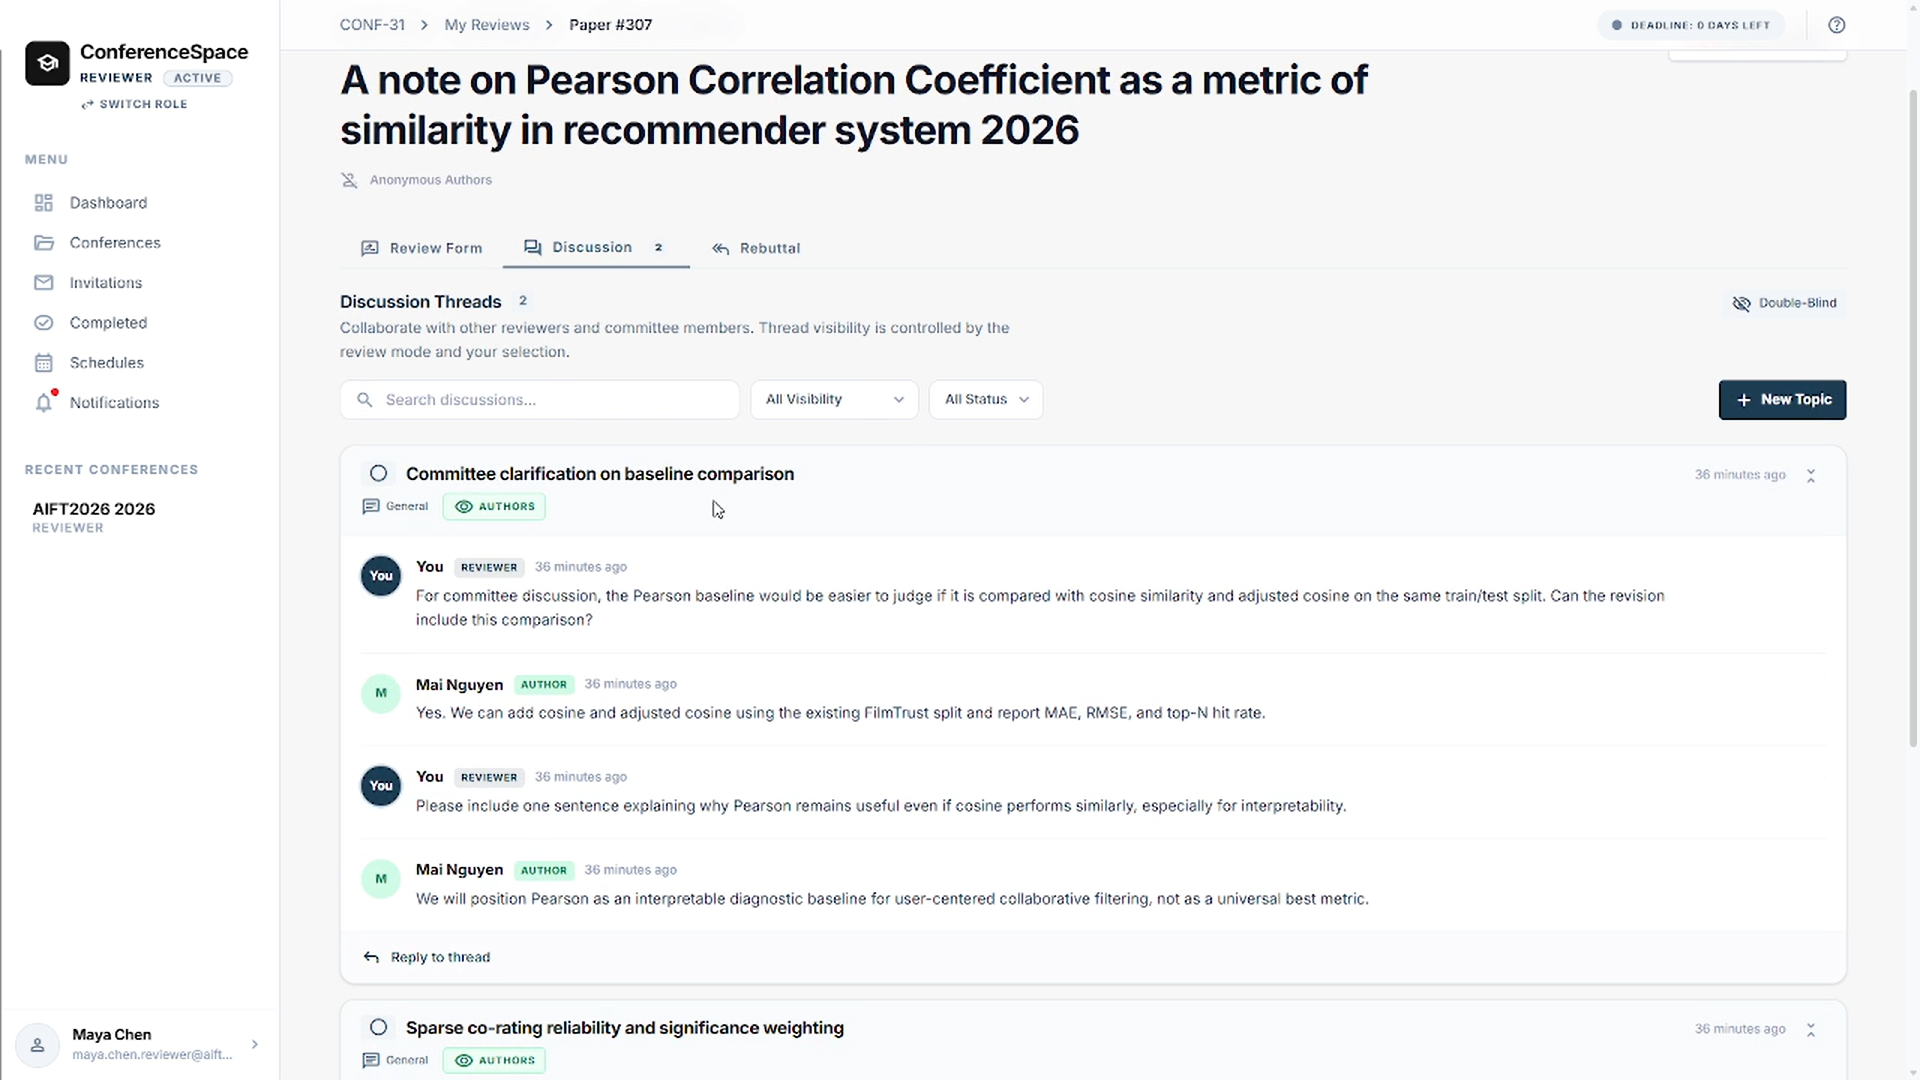
\includegraphics[width=0.95\textwidth]{images/chapter_3_uc08_discussion_chat.png}
  \caption{Giao diện hiển thị danh sách và trao đổi nội dung thảo luận}
  \label{fig:uc08-discussion-chat-cut}
\end{figure}

Hình~\ref{fig:uc08-discussion-chat-cut} thể hiện giao diện hiển thị danh sách chủ đề và nội dung trao đổi trong từng chủ đề.

\subsubsection{UC-09. Tổng hợp bằng chứng hỗ trợ Chủ tọa ra quyết định}

Backend tập hợp điểm số, bản phản biện, phản hồi của Tác giả, thay đổi sau phản hồi và nội dung thảo luận. Chair Decision Copilot tổ chức các nguồn này thành bản tổng hợp gồm điểm đồng thuận, bất đồng, vấn đề còn mở và bằng chứng liên quan. Chủ tọa đối chiếu bản tổng hợp với dữ liệu gốc rồi tự ghi nhận quyết định cuối cùng. Khi bộ bằng chứng thay đổi, hệ thống đánh dấu kết quả cũ là không còn hiệu lực.

\begin{figure}[H]
  \centering
  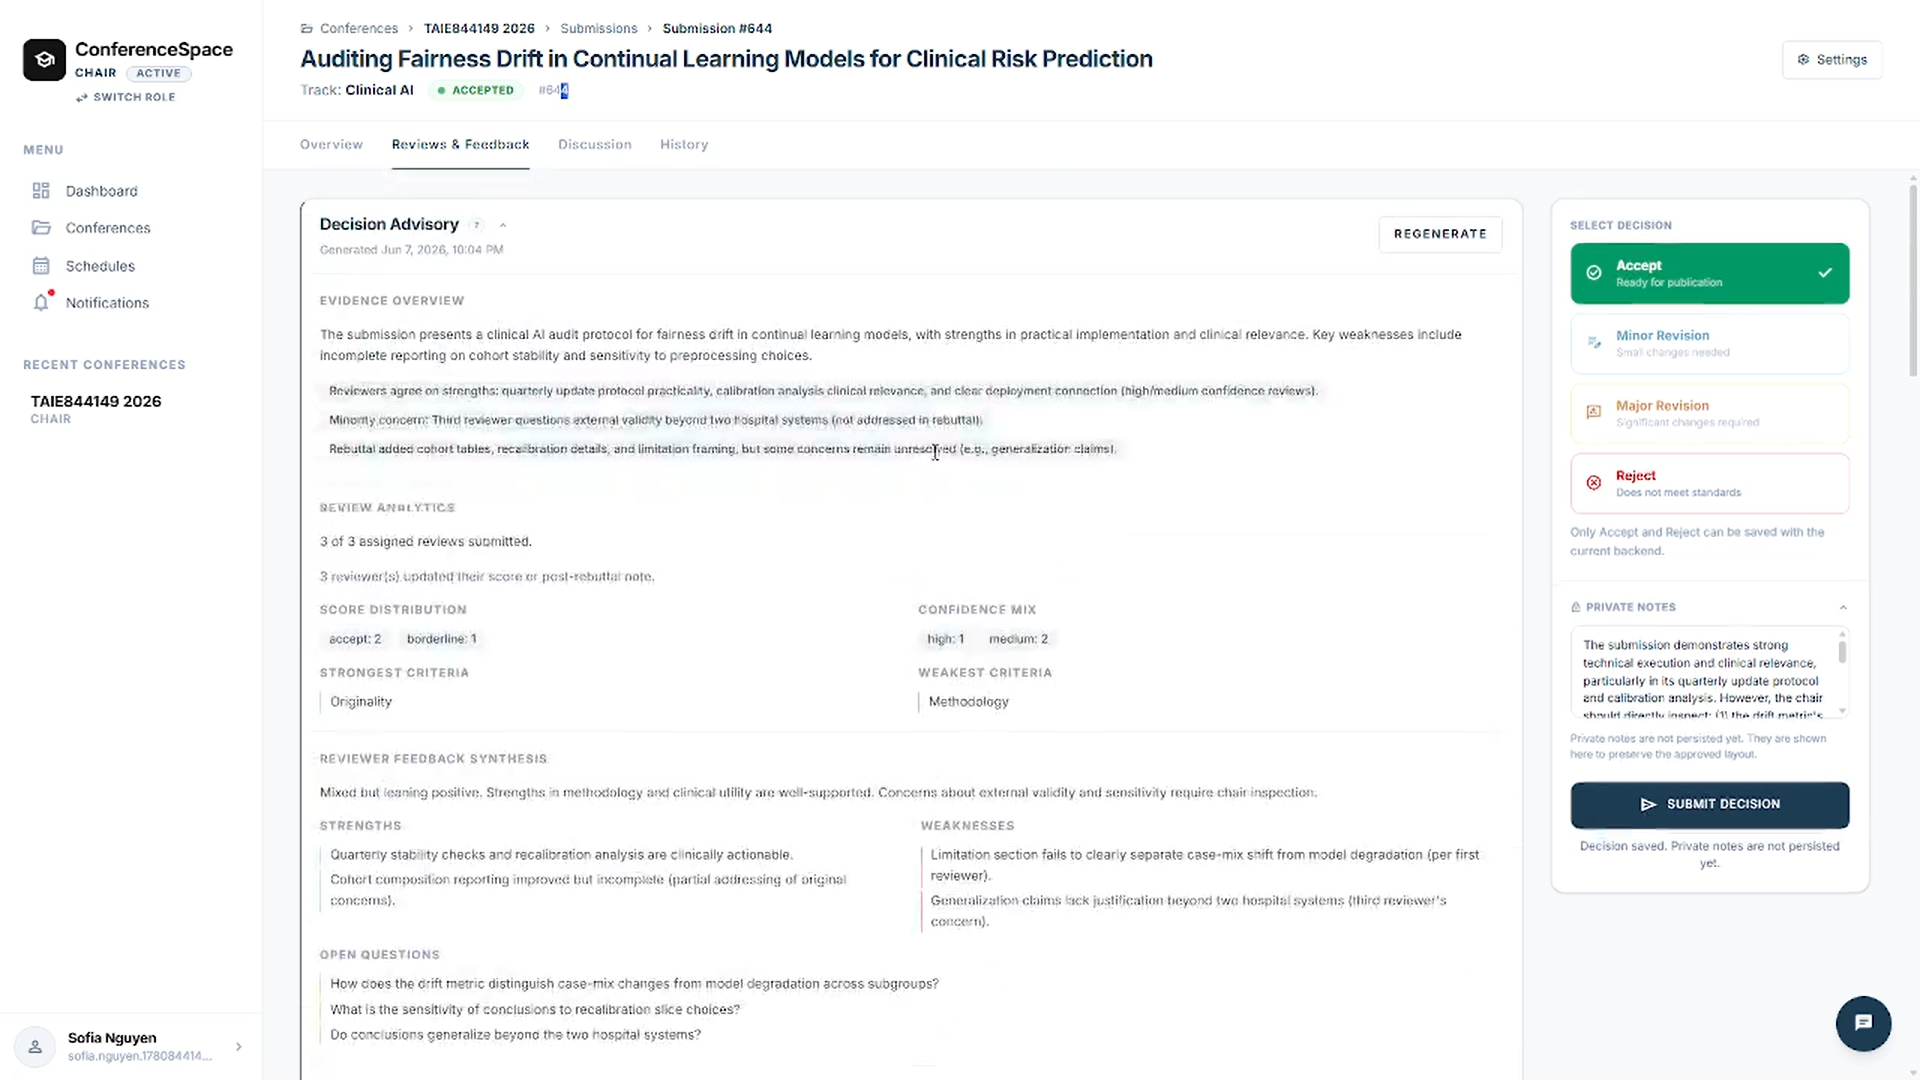
\includegraphics[width=0.95\textwidth]{images/chapter_3_uc09_decision_support.png}
  \caption{Giao diện tổng hợp bằng chứng và ghi nhận quyết định của Chủ tọa}
  \label{fig:uc09-decision-cut}
\end{figure}

Hình~\ref{fig:uc09-decision-cut} minh họa giao diện tổng hợp bằng chứng và ghi nhận quyết định của Chủ tọa.

Chair Decision Copilot không tạo khuyến nghị chấp nhận hoặc từ chối. Khi dịch vụ AI gặp lỗi, Chủ tọa vẫn có thể đọc trực tiếp các nguồn bằng chứng và tiếp tục quy trình nghiệp vụ.

\subsubsection{UC-10. Truy vấn trạng thái và hướng dẫn theo ngữ cảnh bằng Chatbot Agent}

Chatbot Agent nhận câu hỏi, lịch sử hội thoại và ngữ cảnh trang hiện tại. Nếu câu hỏi cần dữ liệu nghiệp vụ, Chatbot Agent gọi công cụ truy vấn để gửi yêu cầu có cấu trúc đến backend; backend kiểm tra mã xác thực, tài nguyên, trường dữ liệu, bộ lọc và quyền của người dùng trước khi trả phần dữ liệu tối thiểu được phép. Chatbot Agent dùng kết quả này để tạo câu trả lời phù hợp với vai trò và không truy cập trực tiếp cơ sở dữ liệu.

Backend từ chối yêu cầu vượt quá quyền truy cập; Chatbot Agent thông báo rõ khi câu hỏi nằm ngoài phạm vi chức năng được hỗ trợ. Khi công cụ gặp lỗi, hệ thống trả trạng thái lỗi thay vì tạo dữ liệu không có căn cứ. Các kịch bản hội thoại ở Chương 4 kiểm tra ranh giới này trong phạm vi tài nguyên và vai trò đã chọn.

\begin{figure}[H]
  \centering
  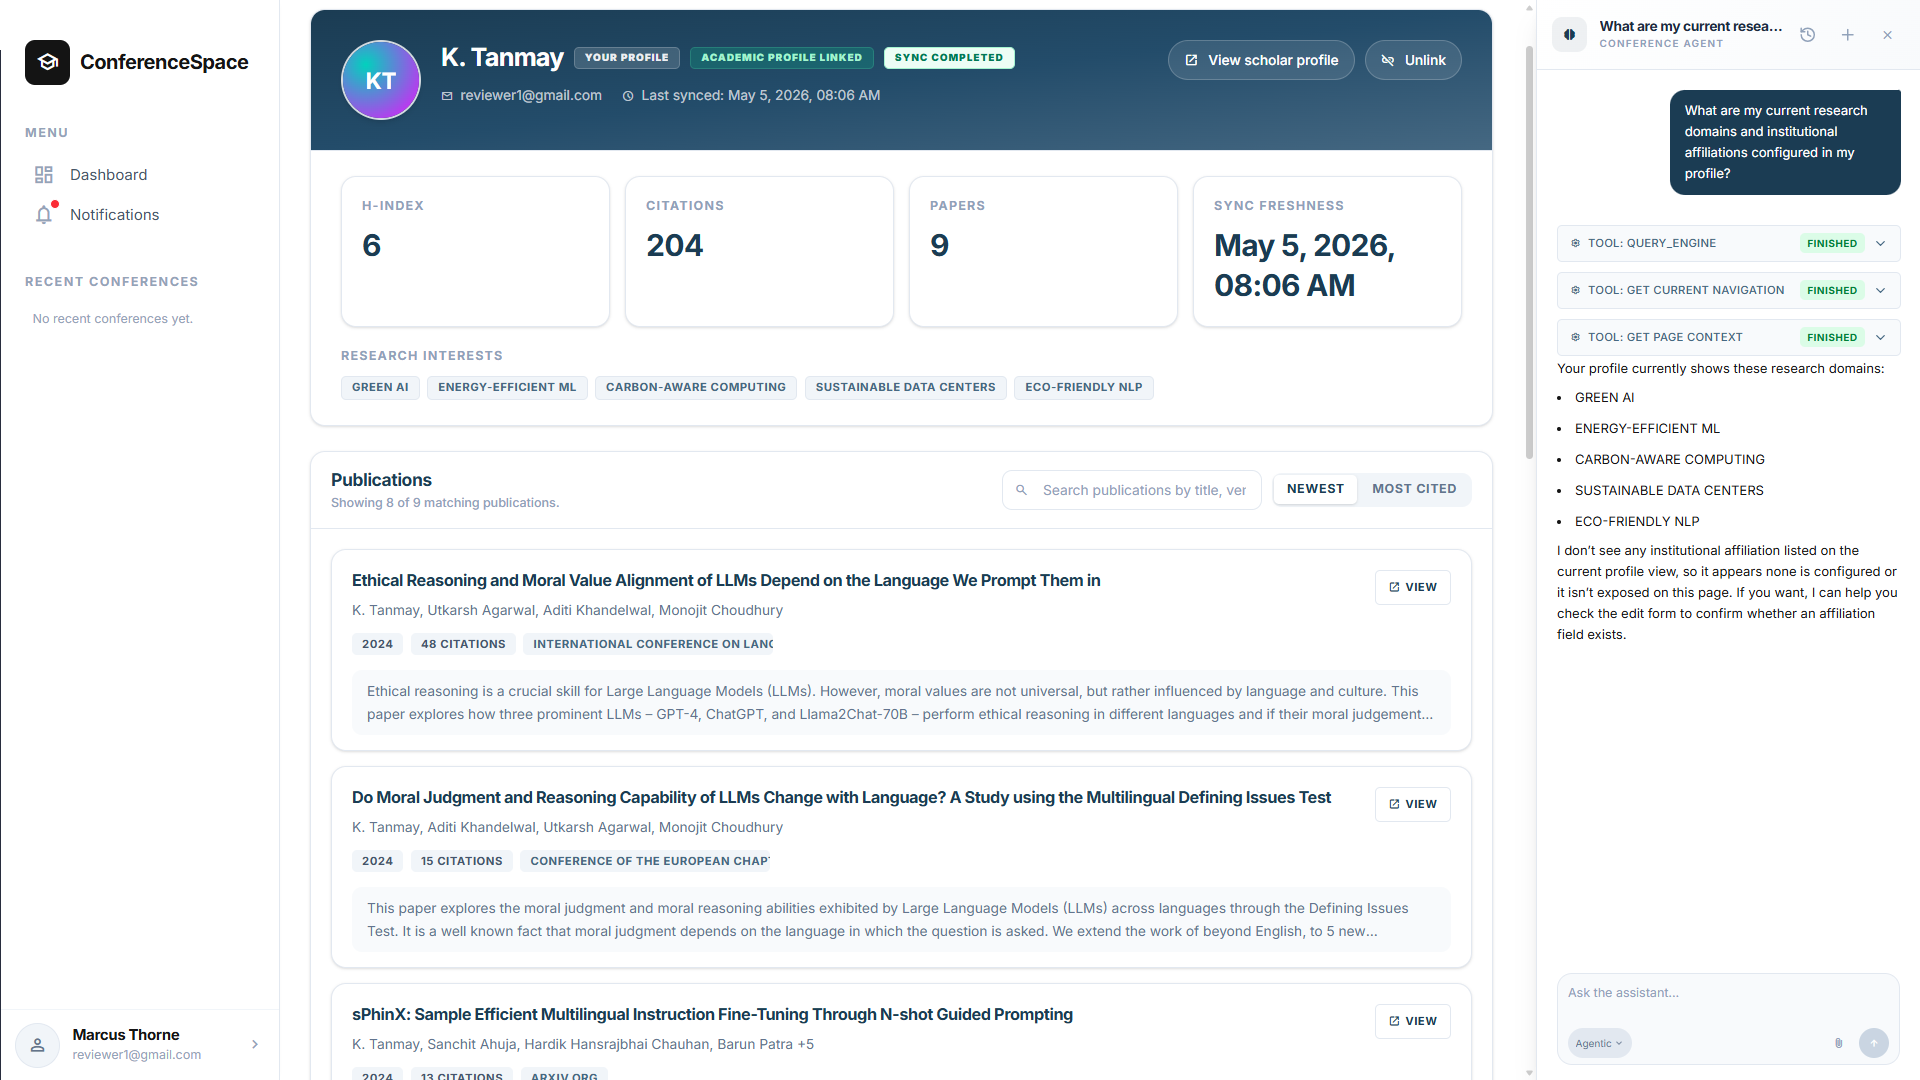
\includegraphics[width=0.95\textwidth]{images/chapter_3_uc10_chatbot_interface.png}
  \caption{Giao diện hội thoại và hỗ trợ tra cứu thông tin của Chatbot Agent}
  \label{fig:uc10-chatbot-cut}
\end{figure}

Hình~\ref{fig:uc10-chatbot-cut} minh họa giao diện hội thoại của Chatbot Agent trong luồng này.

\section{Thiết kế kỹ thuật}

\subsection{Kiến trúc tổng thể}
\label{subsec:ch3-architecture-cut}

ConferenceSpace gồm giao diện web Next.js, backend Go/Gin, dịch vụ AI FastAPI, PostgreSQL, Redis, Neo4j và cổng Caddy. Backend nghiệp vụ là một ứng dụng nguyên khối có kiến trúc phân lớp; nhóm không chia nhỏ nghiệp vụ thành các vi dịch vụ khi chưa có nhu cầu vận hành tương ứng. Dịch vụ AI và các kho dữ liệu được tách tại ranh giới triển khai vì có vòng đời, tải xử lý và yêu cầu truy cập khác với backend.

\begin{figure}[H]
  \centering
  \begin{adjustbox}{max width=\textwidth}
    \begin{tikzpicture}[node distance=12mm and 18mm, >=Latex]
      \node[prismNode] (browser) at (0,0) {Trình duyệt};
      \node[prismNode] (caddy) at (0,-2.2) {Caddy};
      \node[prismNode] (web) at (0,-4.4) {Next.js};
      \node[prismNode] (backend) at (0,-6.6) {Backend Go/Gin};
      \node[prismNode] (postgres) at (-6.4,-9.2) {PostgreSQL};
      \node[prismNode] (neo4j) at (-2.1,-9.2) {Neo4j};
      \node[prismNode] (ai) at (2.1,-9.2) {Dịch vụ AI};
      \node[prismNode] (external) at (6.4,-9.2) {Nguồn dữ liệu học thuật bên ngoài};
      \node[prismNode] (redis) at (0,-11.8) {Redis};
      \node[prismNode] (model) at (4.3,-11.8) {Nhà cung cấp mô hình};
      \draw[prismArrow] (browser) -- (caddy);
      \draw[prismArrow] (caddy) -- (web);
      \draw[prismArrow] (web) -- (backend);
      \draw[prismArrow] (web) -- node[prismEdgeLabel] {API hội thoại} (ai);
      \draw[prismArrow] (backend) -- (postgres);
      \draw[prismArrow] (backend) -- (neo4j);
      \draw[prismArrow] (backend) -- (ai);
      \draw[prismDashedArrow, bend left=24] (ai) to node[prismEdgeLabel] {endpoint truy vấn của backend} (backend);
      \draw[prismArrow] (backend) -- (external);
      \draw[prismArrow] (ai) -- (redis);
      \draw[prismArrow] (ai) -- (model);
      \draw[prismDashedArrow] (ai) -- node[prismEdgeLabel] {kết quả cần truy vết} (postgres);
    \end{tikzpicture}
  \end{adjustbox}
  \caption{Kiến trúc dịch vụ và ranh giới dữ liệu của ConferenceSpace}
  \label{fig:ch3-architecture-cut}
\end{figure}

Backend là ranh giới nghiệp vụ chính đối với dữ liệu và cập nhật trạng thái. Giao diện không truy cập trực tiếp cơ sở dữ liệu hoặc nhà cung cấp mô hình; tuy nhiên, Next.js có luồng giao tiếp trực tiếp với dịch vụ AI cho hội thoại. Khi Chatbot Agent cần dữ liệu nghiệp vụ, dịch vụ AI gọi endpoint truy vấn của backend bằng mã xác thực của người dùng và mã xác thực liên dịch vụ; backend tiếp tục kiểm tra danh mục tài nguyên và phân quyền theo vai trò trong hội nghị (RBAC). Sơ đồ vì vậy tách luồng hội thoại Next.js--AI khỏi luồng truy vấn dữ liệu AI--backend.

\subsection{Thiết kế giao diện web và trải nghiệm theo vai trò}
\label{subsec:ch3-web-cut}

Giao diện được tổ chức theo không gian làm việc của từng vai trò. Không gian Tác giả kết nối hoạt động khám phá hội nghị, nộp và quản lý bài; không gian Phản biện viên kết nối lời mời, bài được phân công, trình soạn phản biện và thảo luận; không gian Chủ tọa kết nối cấu hình, phân công, giám sát tiến độ và ra quyết định. Chatbot Agent và thông báo xuất hiện trong cả ba không gian nhưng dùng cùng ngữ cảnh xác thực và quyền trên tài nguyên.

Giao diện sử dụng Next.js App Router, React, TypeScript, Radix UI và Tailwind CSS \cite{ch3ref1,ch3ref3,ch3ref4,ch3ref5}. Các luồng dài được chia thành từng bước; trạng thái quan trọng được thể hiện bằng nhãn và bảng; thao tác gửi bài, gửi phản biện và lưu quyết định yêu cầu người dùng xác nhận. Đầu ra AI được trình bày dưới dạng bản nháp, cảnh báo hoặc bản tổng hợp cần kiểm tra, thay vì kết luận chính thức.

\subsection{Thiết kế backend, API và phân quyền}
\label{subsec:ch3-backend-cut}

Backend áp dụng kiến trúc phân lớp. Tầng điều khiển tiếp nhận yêu cầu HTTP; tầng dịch vụ thực thi nghiệp vụ; tầng lưu trữ làm việc với PostgreSQL; tầng tích hợp (client) kết nối dịch vụ AI, Neo4j, nguồn dữ liệu học thuật và thư điện tử. Nghiệp vụ phân công được tách thành miền riêng để logic tính điểm, đối sánh và phát hiện xung đột lợi ích có thể được kiểm thử độc lập.

\begin{figure}[H]
  \centering
  \begin{adjustbox}{max width=0.9\textwidth}
    \begin{tikzpicture}[node distance=12mm and 18mm, >=Latex]
      \node[prismNode] (router) at (0,0) {Bộ định tuyến Gin};
      \node[prismNode] (middleware) at (0,-2.2) {Middleware xác thực và ghi nhật ký};
      \node[prismNode] (controller) at (0,-4.4) {Tầng điều khiển};
      \node[prismNode] (service) at (0,-6.6) {Tầng dịch vụ};
      \node[prismNode] (storage) at (-4.2,-9.0) {Tầng lưu trữ};
      \node[prismNode] (assignment) at (0,-9.0) {Miền phân công};
      \node[prismNode] (clients) at (4.2,-9.0) {Tầng tích hợp};
      \node[prismNode] (db) at (-4.2,-11.4) {PostgreSQL};
      \node[prismNode] (coi) at (0,-11.4) {Đối sánh và xung đột lợi ích};
      \node[prismNode] (services) at (4.2,-11.4) {AI, Neo4j, email};
      \draw[prismArrow] (router) -- (middleware);
      \draw[prismArrow] (middleware) -- (controller);
      \draw[prismArrow] (controller) -- (service);
      \draw[prismArrow] (service) -- (storage);
      \draw[prismArrow] (service) -- (assignment);
      \draw[prismArrow] (service) -- (clients);
      \draw[prismArrow] (storage) -- (db);
      \draw[prismArrow] (assignment) -- (coi);
      \draw[prismArrow] (clients) -- (services);
    \end{tikzpicture}
  \end{adjustbox}
  \caption{Kiến trúc phân tầng của backend}
  \label{fig:ch3-backend-cut}
\end{figure}

Hệ thống phân quyền theo vai trò trong từng hội nghị thay vì dùng quyền toàn cục. Một người có thể là Tác giả ở hội nghị này, Phản biện viên ở hội nghị khác và Chủ tọa ở hội nghị thứ ba; do đó, backend kiểm tra cả danh tính người dùng và quan hệ của họ với tài nguyên cụ thể. Bảng~\ref{tab:ch3-discussion-permission-cut} minh họa cách nguyên tắc này được áp dụng cho chức năng thảo luận.

\begin{table}[H]
  \centering
  \caption{Quyền hiện hành trong chức năng thảo luận theo bài nộp}
  \label{tab:ch3-discussion-permission-cut}
  \setlength{\tabcolsep}{2pt}
  \renewcommand{\arraystretch}{1.15}
  \begin{tabularx}{\textwidth}{|P{0.22\textwidth}|Y|Y|Y|}
    \hline
    \TableHeader{Vai trò} & \TableHeader{Tạo chuỗi} & \TableHeader{Xem chuỗi} & \TableHeader{Gửi tin nhắn} \\ \hline
    Phản biện viên được phân công & Có & Các chuỗi do mình tạo trong bài nộp & Có, trong chuỗi do mình tạo \\ \hline
    Tác giả của bài nộp & Không & Các chuỗi gắn với bài của mình & Có, trong chuỗi liên quan \\ \hline
    Chủ tọa/Đồng chủ tọa & Không & Toàn bộ chuỗi và tin nhắn của bài & Không \\ \hline
  \end{tabularx}
\end{table}

Ngoài JWT dành cho người dùng cuối, hệ thống dùng mã xác thực riêng cho tác vụ quản trị nội bộ và giao tiếp giữa dịch vụ AI với endpoint truy vấn của backend. Mã xác thực dịch vụ không thay thế kiểm tra quyền: backend vẫn giới hạn tài nguyên, trường dữ liệu và thao tác theo người dùng hiện tại.

\subsection{Thiết kế cơ sở dữ liệu và lưu trữ dữ liệu}

ConferenceSpace phân chia dữ liệu theo yêu cầu giao dịch và kiểu truy vấn. PostgreSQL lưu dữ liệu nghiệp vụ, phiên và tin nhắn hội thoại cùng kết quả cần truy vết; Neo4j lưu quan hệ đồng tác giả để truy vấn nhiều bậc; Redis lưu kết quả công cụ đang chờ và bộ đếm giới hạn tần suất có thời hạn ngắn. Bảng~\ref{tab:ch3-db-groups-cut} tóm tắt bốn nhóm dữ liệu chính và vai trò của chúng.

\begingroup
\setlength{\tabcolsep}{2pt}
\begin{longtable}{|P{0.27\textwidth}|P{0.30\textwidth}|P{0.35\textwidth}|}
  \caption{Nhóm dữ liệu chính trong thiết kế cơ sở dữ liệu}\label{tab:ch3-db-groups-cut}\\
  \hline
  \TableHeader{Nhóm dữ liệu} & \TableHeader{Thực thể tiêu biểu} & \TableHeader{Vai trò trong thiết kế} \\ \hline
  \endfirsthead
  \hline
  \TableHeader{Nhóm dữ liệu} & \TableHeader{Thực thể tiêu biểu} & \TableHeader{Vai trò trong thiết kế} \\ \hline
  \endhead
  Nghiệp vụ hội nghị & \textit{conferences}, \CodeBreak{conference\_submissions}, \CodeBreak{paper\_assignments}, \CodeBreak{rebuttal\_points} & Bảo toàn vòng đời nộp bài--phản biện--phản hồi và các ràng buộc giao dịch \\ \hline
  Phân quyền và phối hợp & \textit{users}, \CodeBreak{conference\_user\_roles}, \CodeBreak{discussion\_threads}, \textit{notifications} & Giới hạn thao tác theo vai trò, tài nguyên và chuyển thông báo đến đúng người \\ \hline
  Học thuật và xung đột lợi ích & \CodeBreak{scholar\_profiles}, \CodeBreak{scholar\_papers}, \CodeBreak{coi\_relationships}, đồ thị Neo4j & Phát hiện quan hệ có nguy cơ gây xung đột và lưu bằng chứng để Chủ tọa kiểm tra \\ \hline
  Kết quả AI và kiểm toán & \textit{ai.*\_runs}, \textit{ai.*\_artifacts}, \textit{ai.*\_stage\_records}, \textit{ai\_tool\_audit} & Theo dõi đầu vào, đầu ra, trạng thái và lỗi của từng luồng AI \\ \hline
\end{longtable}
\endgroup

\begin{figure}[H]
  \centering
  \begin{adjustbox}{max width=\textwidth}
    \begin{tikzpicture}[
        entity/.style={draw=black!65, rounded corners=2pt, align=center, font=\scriptsize\ttfamily, text width=3.5cm, minimum height=9mm, fill=green!6},
        fk/.style={-{Latex[length=1.8mm]}, thick, draw=black!75},
        logical/.style={-{Latex[length=1.8mm]}, thick, dashed, draw=blue!65!black},
        relLabel/.style={font=\scriptsize, align=center, fill=white, inner sep=1pt},
        legend/.style={draw=black!45, rounded corners=2pt, align=left, font=\scriptsize, fill=white, inner sep=3pt}
      ]
      \node[entity] (users) at (-7.2,0) {users};
      \node[entity] (conferences) at (-2.4,0) {conferences};
      \node[entity] (roles) at (2.4,0) {conference\_user\_roles};
      \node[entity] (sessions) at (7.2,0) {ai\_sessions / ai\_messages};

      \node[entity] (scholar) at (-7.2,-2.4) {scholar\_profiles};
      \node[entity] (submissions) at (-2.4,-2.4) {conference\_submissions};
      \node[entity] (reviewers) at (2.4,-2.4) {conference\_reviewers};
      \node[entity] (coi) at (7.2,-2.4) {coi\_relationships};

      \node[entity] (rebuttal) at (-7.2,-4.8) {rebuttal\_points};
      \node[entity] (assignments) at (-2.4,-4.8) {paper\_assignments};
      \node[entity] (audit) at (2.4,-4.8) {review\_audit\_events};
      \node[entity] (threads) at (7.2,-4.8) {discussion\_threads};
      \node[entity] (messages) at (7.2,-7.2) {discussion\_messages};

      \draw[fk] (users) -- node[relLabel] {1:0..1} (scholar);
      \draw[fk] (submissions) -- node[relLabel] {1:N} (assignments);
      \draw[fk] (reviewers) -- node[relLabel, pos=0.58] {1:N} (assignments);
      \draw[fk] (assignments) -- node[relLabel] {1:N} (audit);
      \draw[fk] (submissions.east) -- ++(0.8,0) |- node[relLabel, pos=0.73] {1:N} (threads.west);
      \draw[fk] (threads) -- node[relLabel] {1:N} (messages);

      \draw[logical] (users) -- node[relLabel] {định danh} (roles);
      \draw[logical] (conferences) -- node[relLabel] {phạm vi} (roles);
      \draw[logical] (conferences) -- node[relLabel] {phạm vi} (submissions);
      \draw[logical] (users.south east) to[bend left=14] node[relLabel, pos=0.55] {vai trò} (reviewers.north west);
      \draw[logical] (conferences.south east) -- node[relLabel] {phạm vi} (reviewers.north west);
      \draw[logical] (submissions) -- node[relLabel] {định danh} (rebuttal);
      \draw[logical] (submissions.east) to[bend left=12] node[relLabel, pos=0.72] {định danh} (coi.west);
      \draw[logical] (reviewers) -- node[relLabel] {định danh} (coi);
      \draw[logical] (users) -- node[relLabel] {định danh} (sessions);

      \node[legend, anchor=north west] at (-7.2,-7.0) {
        \tikz\draw[fk] (0,0) -- (0.9,0);\; khóa ngoại được PostgreSQL cưỡng chế\\[2pt]
        \tikz\draw[logical] (0,0) -- (0.9,0);\; quan hệ logic qua định danh hoặc tầng ứng dụng
      };
    \end{tikzpicture}
  \end{adjustbox}
  \caption{Các thực thể triển khai và quan hệ chính trong PostgreSQL}
  \label{fig:ch3-data-cut}
\end{figure}

Hình~\ref{fig:ch3-data-cut} giữ nguyên định danh kỹ thuật và phân biệt khóa ngoại vật lý với quan hệ được nối ở tầng ứng dụng. \CodeBreak{paper\_assignments.reviewer\_id} tham chiếu \CodeBreak{conference\_reviewers.id}; từ đó hệ thống mới xác định người dùng giữ vai trò Phản biện viên trong một hội nghị. Nét đứt không biểu thị ràng buộc khóa ngoại trong PostgreSQL. \CodeBreak{coi\_relationships} lưu bằng chứng do quy trình refresh hoặc rebuild tạo ra, còn bản đồ xung đột dùng để loại cặp xung đột được xây dựng riêng cho từng lượt đối sánh.

Reviewer Initial Analysis và Chair Decision Copilot dùng mã nhận diện đầu vào (fingerprint) để phát hiện kết quả không còn hiệu lực (\textit{stale}) khi dữ liệu nguồn thay đổi. Reviewer Initial Analysis tính mã này từ trạng thái bài nộp; Chair Decision Copilot tính mã cho bộ bằng chứng và từng thành phần, đồng thời lưu lý do hết hiệu lực. Submission Gating ghi mã nhận diện đầu vào cùng mã chính sách cho mỗi lần chạy, còn Review Quality Auditor lưu yêu cầu, phản hồi, trạng thái lần chạy và mã nhận diện của điều kiện phát hiện.

Submission Autofill không lưu kết quả theo cơ chế hết hiệu lực mà trả dữ liệu để Tác giả áp dụng vào biểu mẫu có thể chỉnh sửa. Chatbot Agent lưu phiên và lịch sử hội thoại để phục vụ truy vết.

\subsection{Luồng xử lý hệ thống}

\subsubsection{Luồng nộp bài có AI hỗ trợ}

Trong luồng nộp bài, giao diện chuyển tệp và ngữ cảnh hội nghị đến backend; backend gọi Submission Autofill để tạo bản nháp, sau đó lưu các chỉnh sửa do Tác giả xác nhận. Trước khi gửi chính thức, backend gửi bản nháp hiện hành đến Submission Gating để kiểm tra. AI chỉ tạo dữ liệu hỗ trợ và cảnh báo; backend kiểm soát việc ghi dữ liệu chính thức, còn Tác giả quyết định gửi bài. Tác giả có thể tiếp tục nhập và lưu bản nháp khi chức năng AI không khả dụng; thao tác gửi bài vẫn cần một kết quả Submission Gating hợp lệ.

\subsubsection{Luồng Chatbot Agent truy vấn dữ liệu hệ thống}

Chatbot Agent chỉ gọi endpoint truy vấn mà backend đã định nghĩa và cho phép sử dụng. Mỗi yêu cầu gồm ngữ cảnh người dùng, tài nguyên, trường dữ liệu và điều kiện truy vấn; backend xác thực người dùng và dịch vụ, kiểm tra danh mục tài nguyên rồi mới thực thi. Cách tổ chức này giữ việc kiểm soát quyền tại backend và ngăn Chatbot Agent sử dụng quyền truy cập cơ sở dữ liệu trực tiếp.

\section{Cơ chế nghiệp vụ và thuật toán xác định}

\subsection{Vai trò của các cơ chế xác định}

Các tác vụ có quy tắc rõ ràng được tách khỏi lớp AI để người dùng có thể kiểm tra điều kiện và nguyên nhân của kết quả. Nhóm này gồm đối sánh Phản biện viên, phát hiện xung đột lợi ích, kiểm soát trạng thái và hạn chót nộp bài, phân quyền, định tuyến thông báo và kiểm tra cấu trúc dữ liệu. Kết quả chỉ ổn định khi hệ thống đã định nghĩa đầy đủ quy tắc, bao gồm cách phân xử các trường hợp bằng điểm.

\subsection{Đối sánh phản biện viên}
\label{subsec:ch3-matching-cut}

Hệ thống tạo đề xuất phân công từ miền chuyên môn của bài nộp và Phản biện viên, cấu hình hội nghị cùng kết quả kiểm tra xung đột lợi ích. Matcher hiện chỉ nhận đầu vào là định danh Phản biện viên, không kèm dữ liệu tải hiện có; do đó bộ đếm tải được khởi tạo bằng $0$ và chỉ phản ánh số phân công phát sinh trong lượt chạy, không bao gồm các phân công đã tồn tại trước đó. Với tập miền chuyên môn của bài nộp $S$ và của Phản biện viên $R$, điểm phù hợp được tính bằng hệ số Jaccard:

\[
  J(S,R)=\frac{|S\cap R|}{|S\cup R|}.
\]

Nếu cả hai tập rỗng, hệ thống gán điểm $0$ vì không có bằng chứng về mức độ phù hợp. Nhóm chọn Jaccard vì điểm số có thể giải thích trực tiếp từ số miền chuyên môn chung và không cần mô hình học máy hoặc dữ liệu huấn luyện. Chiến lược tham lam lần lượt chọn các cặp có điểm cao, nhờ đó đơn giản hóa việc triển khai và kiểm tra so với việc giải bài toán tối ưu toàn cục. Đổi lại, Jaccard xem các miền chuyên môn như tập hợp không trọng số; chiến lược tham lam có thể bỏ lỡ phương án có tổng mức phù hợp cao hơn cho toàn bộ hội nghị và phụ thuộc vào thứ tự khi nhiều cặp bằng điểm.

Hình~\ref{fig:ch3-matching-flow-cut} biểu diễn hai lượt của thuật toán và ràng buộc được giữ hoặc nới ở mỗi lượt.

\begin{figure}[H]
  \centering
  \begin{adjustbox}{max width=0.90\textwidth, max height=0.70\textheight, keepaspectratio}
    \begin{tikzpicture}[scale=0.84, every node/.style={transform shape},
        matchStep/.style={draw=black!65, rounded corners=2pt, align=center, font=\footnotesize, text width=4.2cm, minimum height=11mm, fill=blue!7},
        pass/.style={draw=black!65, rounded corners=2pt, align=left, font=\footnotesize, text width=5.5cm, minimum height=20mm, fill=green!7},
        decision/.style={draw=black!65, diamond, aspect=2.2, align=center, font=\scriptsize, text width=2.8cm, fill=orange!9},
        end/.style={draw=black!65, rounded corners=2pt, align=center, font=\footnotesize, text width=4.6cm, minimum height=11mm, fill=gray!9},
        >=Latex
      ]
      \node[matchStep] (matrix) at (0,0) {Tạo ma trận điểm Jaccard cho các cặp bài nộp--Phản biện viên};
      \node[matchStep] (filter) at (0,-2.2) {Loại các cặp có xung đột lợi ích};
      \node[matchStep] (sort) at (0,-4.4) {Sắp xếp điểm giảm dần\\chưa có tiêu chí phân xử khi bằng điểm};
      \node[pass] (pass1) at (0,-7.3) {\textbf{Lượt 1}\newline Giữ ngưỡng điểm, số người cần cho mỗi bài, giới hạn tải phát sinh trong lượt chạy và xung đột lợi ích};
      \node[decision] (unassigned) at (0,-10.7) {Bài nào vẫn có 0 Phản biện viên?};
      \node[pass] (pass2) at (5.8,-13.8) {\textbf{Lượt 2}\newline Bỏ ngưỡng điểm và giới hạn tải; vẫn giữ xung đột lợi ích; chỉ bổ sung một Phản biện viên};
      \node[end] (result) at (0,-17.0) {Trả đề xuất, điểm số và danh sách bài còn thiếu người};
      \node[end, fill=orange!7] (confirm) at (0,-19.4) {Chủ tọa xem, điều chỉnh và xác nhận};
      \draw[prismArrow] (matrix) -- (filter);
      \draw[prismArrow] (filter) -- (sort);
      \draw[prismArrow] (sort) -- (pass1);
      \draw[prismArrow] (pass1) -- (unassigned);
      \draw[prismArrow] (unassigned) -- node[prismEdgeLabel] {Có} (pass2);
      \draw[prismArrow] (unassigned) -- node[prismEdgeLabel] {Không} (result);
      \draw[prismArrow] (pass2) -- (result);
      \draw[prismArrow] (result) -- (confirm);
    \end{tikzpicture}
  \end{adjustbox}
  \caption{Hai lượt của thuật toán đối sánh GreedyMatcher}
  \label{fig:ch3-matching-flow-cut}
\end{figure}

Lượt dự phòng có thể chọn cặp có điểm bằng $0$ hoặc làm Phản biện viên vượt giới hạn tải trong lượt chạy; thủ tục cũng không bảo đảm mọi bài có đủ số người yêu cầu. Vì vậy, đầu ra gồm điểm, lý do, số phân công được tạo cho từng Phản biện viên và danh sách bài còn thiếu người để Chủ tọa kiểm tra trước khi xác nhận. Do chưa có tiêu chí phân xử thứ cấp khi bằng điểm và chưa tính đến tải lịch sử của Phản biện viên, báo cáo không dùng thuật toán này làm bằng chứng cho tính tái tạo hoàn toàn hoặc cân bằng tổng tải hiện có.

\begin{table}[H]
  \centering
  \caption{Tình huống ngoại lệ trong đối sánh Phản biện viên}
  \label{tab:ch3-matching-exceptions-cut}
  \setlength{\tabcolsep}{3pt}
  \renewcommand{\arraystretch}{1.15}
  \begin{tabularx}{\textwidth}{|Y|Y|}
    \hline
    \TableHeader{Tình huống} & \TableHeader{Cách xử lý} \\ \hline
    Bài nộp không có đủ Phản biện viên không có xung đột lợi ích & Đánh dấu thiếu để Chủ tọa mời thêm hoặc phân công thủ công \\ \hline
    Hồ sơ thiếu miền chuyên môn & Giữ ứng viên với điểm thấp nếu không có xung đột lợi ích, nhưng không ưu tiên \\ \hline
    Không cấu hình kết nối Neo4j & Áp dụng các lớp kiểm tra còn lại và ghi trạng thái \CodeBreak{skipped\_neo4j\_unavailable}; độ bao phủ quan hệ bị giảm \\ \hline
    Tất cả ứng viên có điểm phù hợp đều có xung đột lợi ích & Thuật toán tự động không gán và giữ bài nộp trong danh sách thiếu Phản biện viên \\ \hline
  \end{tabularx}
\end{table}

Thuật toán tự động tạo danh sách đề xuất và cung cấp căn cứ để Chủ tọa kiểm tra trước khi xác nhận. Bộ đếm tải chỉ bao gồm các phân công phát sinh trong lượt chạy hiện tại, còn trường hợp bằng điểm chưa có tiêu chí phân xử thứ cấp; đây là hai ranh giới trực tiếp của phương án hiện hành.

\subsection{Phát hiện xung đột lợi ích}
\label{subsec:ch3-coi-cut}

Hệ thống kiểm tra xung đột lợi ích theo ba nguồn bổ sung cho nhau: quan hệ tác giả của bài, khai báo thủ công và quan hệ đồng tác giả nhiều bậc trong Neo4j. \CodeBreak{coi\_relationships} lưu bằng chứng đã phát hiện để Chủ tọa kiểm tra, còn bản đồ xung đột được tạo cho lượt đối sánh là dữ liệu trực tiếp quyết định cặp nào bị loại khỏi thuật toán tự động. Hai cấu trúc phục vụ hai mục đích khác nhau và không được xem là thay thế cho nhau.

\begin{figure}[H]
  \centering
  \begin{adjustbox}{max width=\textwidth}
    \begin{tikzpicture}[
        source/.style={draw=black!65, rounded corners=2pt, align=center, font=\footnotesize, text width=3.5cm, minimum height=12mm, fill=blue!7},
        process/.style={draw=black!65, rounded corners=2pt, align=center, font=\footnotesize, text width=4.5cm, minimum height=13mm, fill=green!7},
        warning/.style={draw=black!65, rounded corners=2pt, align=center, font=\footnotesize, text width=4.7cm, minimum height=13mm, fill=orange!9},
        evidence/.style={draw=black!65, rounded corners=2pt, align=center, font=\footnotesize, text width=4.7cm, minimum height=13mm, fill=gray!9},
        lane/.style={draw=black!35, rounded corners=3pt, dashed, inner sep=5pt},
        laneTitle/.style={font=\scriptsize\bfseries, anchor=south west},
        >=Latex
      ]
      \node[source] (author) at (-5.2,0) {Tự phản biện và quan hệ đồng tác giả trực tiếp};
      \node[source] (declared) at (0,0) {Xung đột do Tác giả khai báo};
      \node[source] (graph) at (5.2,0) {Quan hệ đồng tác giả nhiều bậc qua Neo4j};

      \node[process] (map) at (-5.2,-3.1) {Tạo bản đồ xung đột cho lượt chạy};
      \node[process] (auto) at (-5.2,-5.8) {Đối sánh tự động loại cặp xung đột lợi ích trong cả hai lượt};

      \node[process] (rebuild) at (0,-3.1) {Tác vụ refresh/rebuild quan hệ xung đột lợi ích};
      \node[evidence] (stored) at (0,-5.8) {Ghi bằng chứng vào \CodeBreak{coi\_relationships}};

      \node[warning] (manualCheck) at (5.2,-3.1) {Đề xuất thủ công kiểm tra trực tiếp và đọc bộ nhớ đệm xung đột lợi ích nếu có};
      \node[warning] (manualResult) at (5.2,-5.8) {Trả \CodeBreak{COIWarning}; lưu trạng thái kiểm tra trong siêu dữ liệu của đề xuất};

      \draw[prismArrow] (author) -- (map);
      \draw[prismArrow] (declared) -- (map);
      \draw[prismArrow] (graph) -- (map);
      \draw[prismArrow] (map) -- (auto);

      \draw[prismArrow] (author) -- (rebuild);
      \draw[prismArrow] (declared) -- (rebuild);
      \draw[prismArrow] (graph) -- (rebuild);
      \draw[prismArrow] (rebuild) -- (stored);

      \draw[prismArrow] (author) -- (manualCheck);
      \draw[prismArrow] (declared) -- (manualCheck);
      \draw[prismDashedArrow] (stored) to[bend right=16] node[prismEdgeLabel] {bộ nhớ đệm nếu có} (manualCheck);
      \draw[prismArrow] (manualCheck) -- (manualResult);

      \node[laneTitle] at (-7.65,-1.7) {Cưỡng chế trong lượt đối sánh};
      \node[laneTitle] at (-2.45,-1.7) {Dữ liệu truy vết bền vững};
      \node[laneTitle] at (2.75,-1.7) {Cảnh báo cho đề xuất thủ công};
    \end{tikzpicture}
  \end{adjustbox}
  \caption{Ba luồng sử dụng kết quả phát hiện xung đột lợi ích}
  \label{fig:ch3-coi-flow-cut}
\end{figure}

Hình~\ref{fig:ch3-coi-flow-cut} tách ba mục đích sử dụng kết quả xung đột lợi ích. Bản đồ xung đột chỉ phục vụ lượt đối sánh tự động và loại cặp xung đột trước khi xếp hạng. \CodeBreak{coi\_relationships} được cập nhật qua tác vụ refresh hoặc rebuild riêng. Khi Chủ tọa thêm đề xuất thủ công, backend kiểm tra trực tiếp quan hệ tác giả, đồng tác giả và khai báo, đọc thêm bộ nhớ đệm xung đột lợi ích nếu có, trả \CodeBreak{COIWarning} và lưu trạng thái kiểm tra trong siêu dữ liệu của đề xuất; thao tác này không tự ghi quan hệ mới vào \CodeBreak{coi\_relationships}.

Thuật toán tự động không nới lỏng ràng buộc xung đột lợi ích trong lượt dự phòng. Khi thành phần phát hiện quan hệ chưa được cấu hình, hệ thống ghi \CodeBreak{skipped\_neo4j\_unavailable} và tiếp tục bằng các nguồn còn lại. Nếu truy vấn Neo4j thất bại, một số luồng chỉ ghi nhật ký lỗi rồi tiếp tục; khi đó, hệ thống không thể khẳng định rằng quan hệ đồng tác giả nhiều bậc đã được kiểm tra đầy đủ. Luồng thêm đề xuất thủ công hiện chỉ cảnh báo, chưa chặn ghi dữ liệu và chưa lưu bản ghi kiểm toán riêng cho quyết định tiếp tục.

\subsection{Các cơ chế nghiệp vụ hỗ trợ vận hành}
\label{subsec:ch3-operations-cut}

Các cơ chế hỗ trợ gồm máy trạng thái của hội nghị, kiểm soát hạn chót nộp bài, phân quyền theo vai trò trong hội nghị (RBAC), định tuyến thông báo và kiểm tra cấu trúc dữ liệu. Các cơ chế này kiểm tra và giới hạn thao tác theo vai trò, trạng thái và quy tắc đã được triển khai trước khi hệ thống ghi dữ liệu.

Cơ chế kiểm soát bản thảo hoàn chỉnh hiện chỉ kiểm tra bài ở trạng thái \textit{accepted} và tính hợp lệ của tệp; hệ thống chưa kiểm tra hạn chót nộp bản thảo hoàn chỉnh tại thời điểm thực thi. Giới hạn được nêu riêng vì đầu ra AI không thể bù cho một quy tắc nghiệp vụ chưa được áp dụng đầy đủ.

\section{Giải pháp AI}

\subsection{Vai trò của AI trong hệ thống}

AI được tích hợp vào sáu luồng hỗ trợ: Submission Autofill hỗ trợ nhập liệu; Submission Gating hỗ trợ kiểm tra bài nộp; Reviewer Initial Analysis hỗ trợ định hướng đọc; Review Quality Auditor hỗ trợ rà soát bản nháp; Chair Decision Copilot hỗ trợ tổng hợp bằng chứng; và Chatbot Agent hỗ trợ truy vấn dữ liệu. Bảng~\ref{tab:ch3-ai-overview-cut} đối chiếu đầu ra, điểm kiểm soát và ranh giới của từng luồng.

\begingroup
\setlength{\tabcolsep}{2pt}
\begin{longtable}{|P{0.17\textwidth}|P{0.26\textwidth}|P{0.23\textwidth}|P{0.26\textwidth}|}
  \caption{Dữ liệu và trạng thái của các luồng AI}\label{tab:ch3-ai-overview-cut}\\
  \hline
  \TableHeader{Luồng} & \TableHeader{Đầu vào} & \TableHeader{Đầu ra} & \TableHeader{Lỗi hoặc hiệu lực kết quả} \\ \hline
  \endfirsthead
  \hline
  \TableHeader{Luồng} & \TableHeader{Đầu vào} & \TableHeader{Đầu ra} & \TableHeader{Lỗi hoặc hiệu lực kết quả} \\ \hline
  \endhead
  Submission Autofill & Tệp và ngữ cảnh hội nghị & Siêu dữ liệu nháp, gợi ý chuyên đề & Cảnh báo khi thiếu dữ liệu; chưa lưu kết quả dưới dạng bản ghi có trạng thái \textit{stale} \\ \hline
  Submission Gating & Tệp và chính sách hội nghị & Trạng thái cùng phát hiện có bằng chứng & Ghi mã nhận diện đầu vào và mã chính sách; giữ kết quả kiểm tra theo quy tắc nếu riêng bước AI lỗi \\ \hline
  Reviewer Initial Analysis & Bản thảo và phân công & Bản định hướng đọc & Dùng mã nhận diện đầu vào để chuyển kết quả sang \textit{stale} khi bản thảo thay đổi \\ \hline
  Review Quality Auditor & Bản nháp phản biện và điểm & Danh sách phát hiện & Lưu trạng thái lần chạy và mã nhận diện của điều kiện phát hiện; lỗi thực thi được báo riêng \\ \hline
  Chair Decision Copilot & Bộ bằng chứng & Bản tổng hợp đồng thuận, bất đồng và vấn đề còn mở & Dùng mã nhận diện của bộ bằng chứng để đánh dấu \textit{stale} và nêu lý do \\ \hline
  Chatbot Agent & Câu hỏi, vai trò và ngữ cảnh trang & Câu trả lời cùng kết quả công cụ & Lưu phiên, lịch sử; công khai trạng thái bị từ chối, lỗi hoặc hết thời gian \\ \hline
\end{longtable}
\endgroup

\begin{table}[H]
  \centering
  \caption{Quyền xác nhận và tác động nghiệp vụ của các luồng AI}
  \label{tab:ch3-ai-authority-cut}
  \setlength{\tabcolsep}{3pt}
  \renewcommand{\arraystretch}{1.15}
  \begin{tabularx}{\textwidth}{|P{0.20\textwidth}|Y|Y|}
    \hline
    \TableHeader{Luồng} & \TableHeader{Điểm xác nhận của con người} & \TableHeader{Ranh giới tác động nghiệp vụ} \\ \hline
    Submission Autofill & Tác giả sửa và xác nhận; giao diện lọc chuyên đề hợp lệ & Chỉ cập nhật biểu mẫu, không tự gửi bài \\ \hline
    Submission Gating & Tác giả sửa lỗi hoặc xem cảnh báo & Kiểm tra theo quy tắc có thể tạo \textit{block}; bước đánh giá nội dung bằng AI chỉ tạo \textit{warn} hoặc \textit{pass} \\ \hline
    Reviewer Initial Analysis & Phản biện viên đối chiếu bài gốc & Không cập nhật điểm hoặc nội dung phản biện \\ \hline
    Review Quality Auditor & Phản biện viên xem, sửa hoặc gửi; xác nhận nếu bước rà soát thất bại & Nhãn \textit{blocking} chỉ làm nổi bật phát hiện, không ngăn gửi \\ \hline
    Chair Decision Copilot & Chủ tọa đối chiếu dữ liệu nguồn & Không ghi quyết định chấp nhận hoặc từ chối \\ \hline
    Chatbot Agent & Backend kiểm soát dữ liệu; người dùng xem kết quả & Chỉ đọc dữ liệu được phép, không cập nhật trạng thái chính thức \\ \hline
  \end{tabularx}
\end{table}

\subsection{Các luồng xử lý có sử dụng AI}
\label{subsec:ch3-ai-workflows-cut}

\subsubsection{Submission Autofill}

Submission Autofill đọc bản thảo để tạo bản nháp gồm tiêu đề, tóm tắt, từ khóa, thông tin tác giả và gợi ý chuyên đề. Đầu vào còn gồm ngữ cảnh hội nghị và danh sách chuyên đề đang mở. Cấu trúc phản hồi chưa tự giới hạn giá trị gợi ý vào danh sách này; khi áp dụng kết quả, giao diện đối chiếu và chỉ nhận các chuyên đề còn hợp lệ trong cấu hình hiện hành. Nếu văn bản trích xuất quá ít hoặc thiếu thông tin, luồng trả cảnh báo thay vì suy đoán dữ liệu.

Giao diện giữ toàn bộ trường ở trạng thái có thể chỉnh sửa; backend chỉ lưu bài nộp chính thức sau khi Tác giả xác nhận. Chương 4 đo độ khớp của siêu dữ liệu và kiểm tra gợi ý có thuộc danh sách chuyên đề hợp lệ. Phạm vi đánh giá chưa bao gồm nhãn chuyên gia cho thứ hạng chuyên đề; mức thời gian tiết kiệm được ước tính dựa trên phản hồi tự báo cáo, không phải phép đo trực tiếp thời gian hoàn thành biểu mẫu.

\subsubsection{Submission Gating}

Submission Gating kết hợp kiểm tra theo quy tắc và đánh giá nội dung có AI hỗ trợ. Luồng chuẩn hóa yêu cầu, kiểm tra tính toàn vẹn của tệp, trích xuất tài liệu, xác định dữ kiện, áp dụng chính sách hội nghị và tổng hợp phát hiện thành bốn trạng thái: \textit{pass}, \textit{warn}, \textit{block} hoặc \textit{error}.

\begin{figure}[H]
  \centering
  \begin{adjustbox}{max width=\textwidth}
    \begin{tikzpicture}[
        stage/.style={draw=black!65, rounded corners=2pt, align=center, font=\footnotesize, text width=4.2cm, minimum height=12mm, fill=blue!7},
        rule/.style={draw=black!65, rounded corners=2pt, align=center, font=\footnotesize, text width=4.6cm, minimum height=15mm, fill=green!7},
        ai/.style={draw=black!65, rounded corners=2pt, align=center, font=\footnotesize, text width=4.6cm, minimum height=15mm, fill=orange!9},
        outcome/.style={draw=black!65, rounded corners=2pt, align=center, font=\footnotesize, text width=3.3cm, minimum height=11mm},
        >=Latex
      ]
      \node[stage] (input) at (0,0) {Bản nháp, tệp và chính sách hội nghị};
      \node[stage] (extract) at (0,-2.4) {Kiểm tra tệp, trích xuất tài liệu và xác định dữ kiện};
      \node[rule] (rules) at (-3.7,-5.4) {Kiểm tra theo quy tắc\\định dạng, số trang, phần bắt buộc, ẩn danh và các quy tắc cấu hình};
      \node[ai] (content) at (3.7,-5.4) {Đánh giá nội dung có AI hỗ trợ\\chỉ tạo \textit{warn} hoặc \textit{pass}};
      \node[stage] (merge) at (0,-8.3) {Tổng hợp phát hiện và ghi mã nhận diện đầu vào, mã chính sách};
      \node[outcome, fill=red!7] (block) at (-4.4,-11.0) {\textit{block}\\Lỗi kỹ thuật hoặc vi phạm quy tắc};
      \node[outcome, fill=orange!8] (warn) at (0,-11.0) {\textit{warn}\\Tác giả xem và chỉnh sửa};
      \node[outcome, fill=green!8] (pass) at (4.4,-11.0) {\textit{pass}\\Cho phép tiếp tục};
      \node[outcome, fill=gray!9, text width=4.5cm] (aiError) at (6.2,-8.3) {Bước AI lỗi: giữ kết quả quy tắc và nêu rõ phần nội dung chưa được đánh giá};
      \draw[prismArrow] (input) -- (extract);
      \draw[prismArrow] (extract) -- (rules);
      \draw[prismArrow] (extract) -- (content);
      \draw[prismArrow] (rules) -- (merge);
      \draw[prismArrow] (content) -- (merge);
      \draw[prismDashedArrow] (content) -- (aiError);
      \draw[prismArrow] (aiError) -- (merge);
      \draw[prismArrow] (merge) -- (block);
      \draw[prismArrow] (merge) -- (warn);
      \draw[prismArrow] (merge) -- (pass);
    \end{tikzpicture}
  \end{adjustbox}
  \caption{Submission Gating phân biệt kiểm tra theo quy tắc với cảnh báo nội dung do AI hỗ trợ}
  \label{fig:ch3-gating-flow-cut}
\end{figure}

Hình~\ref{fig:ch3-gating-flow-cut} cho thấy chỉ lỗi kỹ thuật và vi phạm quy tắc mới có thể chặn thao tác gửi. Khi riêng bước đánh giá nội dung lỗi, hệ thống vẫn giữ kết quả của các kiểm tra đã hoàn tất nhưng phải nêu rõ phạm vi chưa được đánh giá.

Các lỗi kỹ thuật và vi phạm quy tắc có thể tái tạo, như tệp không đọc được, thiếu phần bắt buộc, vi phạm yêu cầu ẩn danh hoặc vượt giới hạn trang, tạo trạng thái \textit{block}. Bước đánh giá nội dung bằng AI chỉ tạo \textit{warn} hoặc \textit{pass}; hệ thống không dùng nhận định này để từ chối bài về mặt học thuật. Nếu riêng bước đánh giá nội dung bằng AI gặp lỗi, luồng vẫn có thể tổng hợp kết quả từ các kiểm tra theo quy tắc đã hoàn tất; trạng thái \textit{pass} trong trường hợp này không có nghĩa phần nội dung đã được đánh giá đầy đủ. Nếu toàn bộ quy trình không trả kết quả hợp lệ, backend không tự động cho phép gửi bài. Mỗi phát hiện gồm nguồn, mức độ nghiêm trọng, bằng chứng và hướng dẫn khắc phục để Tác giả biết điều cần kiểm tra.

Mã nhận diện đầu vào và mã chính sách cho biết kết quả được tạo từ bản nháp và cấu hình nào. Chương 4 kiểm tra độ chính xác của tám trường hợp kiểm thử quy tắc và xác nhận 24 trường hợp cảnh báo AI không tạo \textit{block}; bộ thử chưa có nhãn người để đo độ chính xác nội dung của từng cảnh báo.

\subsubsection{Reviewer Initial Analysis}

Reviewer Initial Analysis tạo bản định hướng trước khi Phản biện viên viết nhận xét. Đầu ra gồm tóm tắt, các đóng góp được bài báo trình bày, điểm cần kiểm chứng và chú thích theo từng phần. Kết quả được gắn với phân công, bài nộp và mã nhận diện của trạng thái bài nộp; khi bản thảo thay đổi, hệ thống chuyển bản phân tích cũ sang trạng thái \textit{stale}.

Các nội dung về điểm mạnh, điểm yếu hoặc câu hỏi có thể ảnh hưởng đến nhận định chuyên môn, nên đầu ra không được xem là chỉ dẫn trung lập. Giao diện phải công khai nguồn gốc AI và yêu cầu Phản biện viên đối chiếu với bài gốc. Phạm vi đánh giá ở Chương 4 tập trung vào đầu ra của chức năng, chưa bao gồm số lần đọc lại, tải nhận thức, mức phụ thuộc vào gợi ý hoặc thay đổi trong nội dung phản biện. Vì vậy, kết quả không được dùng để suy ra mức cải thiện chất lượng quyết định chuyên môn.

\subsubsection{Review Quality Auditor}

Review Quality Auditor nhận bản nháp phản biện, điểm số và các định danh cần thiết để phát hiện vấn đề về độ cụ thể, mức độ dựa trên bằng chứng, tính nhất quán và các phần bắt buộc. Ở phiên bản được triển khai, đầu vào không bao gồm đầy đủ toàn văn bài nộp và toàn bộ chính sách hội nghị. Luồng không đánh giá chất lượng học thuật của bài và không tự thay đổi điểm, khuyến nghị hoặc mức độ tự tin của Phản biện viên.

\begin{table}[H]
  \centering
  \caption{Ý nghĩa trạng thái của Review Quality Auditor}
  \label{tab:ch3-rqa-states-cut}
  \setlength{\tabcolsep}{2pt}
  \renewcommand{\arraystretch}{1.15}
  \begin{tabularx}{\textwidth}{|P{0.14\textwidth}|Y|Y|}
    \hline
    \TableHeader{Trạng thái} & \TableHeader{Điều kiện} & \TableHeader{Hành vi trong luồng} \\ \hline
    \textit{pass} & Không có phát hiện đáng kể & Hiển thị kết quả và cho phép tiếp tục lưu hoặc gửi \\ \hline
    \textit{warn} & Có vấn đề cần xem lại & Hiển thị cảnh báo; Phản biện viên có thể sửa hoặc tiếp tục \\ \hline
    \textit{block} & Có ít nhất một phát hiện mà hệ thống gắn nhãn \textit{blocking} & Làm nổi bật phát hiện nghiêm trọng nhưng không ngăn gửi chính thức \\ \hline
  \end{tabularx}
\end{table}

Hình~\ref{fig:ch3-rqa-flow-cut} tách hai lần chạy và hai loại trạng thái thường bị nhầm lẫn trong luồng này.

\begin{figure}[H]
  \centering
  \begin{adjustbox}{max width=\textwidth}
    \begin{tikzpicture}[
        actor/.style={draw=black!65, rounded corners=2pt, align=center, font=\footnotesize, text width=3.5cm, minimum height=11mm, fill=blue!7},
        run/.style={draw=black!65, rounded corners=2pt, align=center, font=\footnotesize, text width=4.6cm, minimum height=14mm, fill=green!7},
        advisory/.style={draw=black!65, rounded corners=2pt, align=center, font=\footnotesize, text width=4.8cm, minimum height=16mm, fill=orange!8},
        failure/.style={draw=black!65, rounded corners=2pt, align=center, font=\footnotesize, text width=5.2cm, minimum height=16mm, fill=red!6},
        >=Latex
      ]
      \node[actor] (draft) at (0,0) {Bản nháp phản biện};
      \node[run] (preflight) at (-4.2,-2.8) {Giao diện chạy\\\CodeBreak{submit\_preflight}};
      \node[advisory] (findings) at (-4.2,-5.8) {Kết quả tư vấn\\\textit{pass}, \textit{warn}, \textit{block}\\đều cho phép Phản biện viên quyết định tiếp tục};
      \node[actor] (submit) at (0,-8.8) {Yêu cầu gửi chính thức};
      \node[run] (enforce) at (4.2,-2.8) {Backend chạy lại\\\CodeBreak{submit\_enforcement}};
      \node[advisory, fill=green!7] (success) at (2.0,-5.8) {Bước rà soát hoàn tất\\lưu phản biện; nhãn \textit{block} không phải điều kiện từ chối};
      \node[failure] (failure) at (7.4,-5.8) {Bước rà soát không hoàn tất\\trả \CodeBreak{review\_audit\_failed}};
      \node[failure, fill=orange!8] (override) at (7.4,-8.8) {Phản biện viên xác nhận tiếp tục\\lưu \CodeBreak{submit\_override\_after\_audit\_failure}};
      \draw[prismArrow] (draft) -- (preflight);
      \draw[prismArrow] (preflight) -- (findings);
      \draw[prismArrow] (findings) -- (submit);
      \draw[prismArrow] (submit) -- (enforce);
      \draw[prismArrow] (enforce) -- (success);
      \draw[prismArrow] (enforce) -- (failure);
      \draw[prismArrow] (failure) -- (override);
    \end{tikzpicture}
  \end{adjustbox}
  \caption{Hai lần chạy Review Quality Auditor và ranh giới giữa phát hiện tư vấn với lỗi thực thi}
  \label{fig:ch3-rqa-flow-cut}
\end{figure}

Giao diện chạy \CodeBreak{submit\_preflight} để hiển thị các phát hiện trước khi Phản biện viên gửi. Khi nhận yêu cầu gửi chính thức, backend chạy lại \CodeBreak{submit\_enforcement} để xác định tác vụ rà soát có hoàn tất hay không; kết quả lần chạy này không thay thế bảng phát hiện mà giao diện đã nhận từ preflight. Backend không dùng trạng thái \textit{block} làm điều kiện từ chối. Chỉ khi bước rà soát không thể hoàn tất, backend mới trả mã \CodeBreak{review\_audit\_failed}; Phản biện viên có thể xác nhận gửi mà không có kết quả rà soát, và hệ thống lưu sự kiện \CodeBreak{submit\_override\_after\_audit\_failure} kèm lý do.

\subsubsection{Chair Decision Copilot}

Chair Decision Copilot nhận bộ bằng chứng gồm điểm số, bản phản biện, phản hồi của Tác giả, nội dung thảo luận và trạng thái liên quan. Hệ thống tạo mã nhận diện cho bộ dữ liệu và từng thành phần, dùng lại bản tổng hợp khi còn hợp lệ hoặc đánh dấu \textit{stale} kèm lý do khi bằng chứng thay đổi. Đầu ra sắp xếp bằng chứng theo các điểm đồng thuận, bất đồng, vấn đề còn mở và ghi chú nháp để Chủ tọa đối chiếu.

Luồng không tạo khuyến nghị chấp nhận hoặc từ chối. Chủ tọa phải đọc dữ liệu gốc và tự ghi quyết định vào hệ thống nghiệp vụ. Việc tách bản tổng hợp khỏi quyết định cuối cùng giúp bảo toàn thẩm quyền, nhưng không loại bỏ hoàn toàn ảnh hưởng của cách AI lựa chọn hoặc trình bày bằng chứng; phạm vi này được nêu như một giới hạn khi diễn giải kết quả đánh giá.

\subsubsection{Chatbot Agent}

Chatbot Agent hỗ trợ ba vai trò tra cứu hướng dẫn và dữ liệu trạng thái của hệ thống. Công cụ xác định liệu câu hỏi có cần dữ liệu nghiệp vụ; nếu có, nó tạo yêu cầu gồm tài nguyên, trường, điều kiện lọc, phép tổng hợp và giới hạn số dòng. Backend xác thực người dùng và dịch vụ, kiểm tra danh mục tài nguyên cùng phân quyền theo vai trò trong hội nghị (RBAC) rồi mới trả dữ liệu.

\begin{figure}[H]
  \centering
  \begin{adjustbox}{max width=\textwidth}
    \begin{tikzpicture}[
        comp/.style={draw=black!65, rounded corners=2pt, align=center, font=\footnotesize, text width=3.6cm, minimum height=12mm, fill=blue!7},
        guard/.style={draw=black!65, rounded corners=2pt, align=center, font=\footnotesize, text width=4.5cm, minimum height=16mm, fill=orange!9},
        data/.style={draw=black!65, rounded corners=2pt, align=center, font=\footnotesize, text width=3.8cm, minimum height=12mm, fill=green!7},
        >=Latex
      ]
      \node[comp] (user) at (0,0) {Người dùng theo vai trò};
      \node[comp] (next) at (4.5,0) {Next.js server\\endpoint hội thoại};
      \node[comp] (agent) at (9.0,0) {Dịch vụ AI\\Chatbot Agent};
      \node[guard] (backend) at (9.0,-3.3) {Backend query endpoint\\xác thực người dùng và dịch vụ; kiểm tra tài nguyên, trường dữ liệu và phân quyền theo vai trò trong hội nghị (RBAC)};
      \node[data] (postgres) at (4.5,-3.3) {PostgreSQL\\dữ liệu nghiệp vụ};
      \node[data] (answer) at (4.5,-6.3) {Câu trả lời kèm trạng thái công cụ};
      \draw[prismArrow] (user) -- node[prismEdgeLabel] {yêu cầu hội thoại} (next);
      \draw[prismArrow] (next) -- node[prismEdgeLabel] {ngữ cảnh và mã xác thực} (agent);
      \draw[prismArrow] (agent) -- node[prismEdgeLabel, right] {yêu cầu truy vấn có cấu trúc} (backend);
      \draw[prismArrow] (backend) -- node[prismEdgeLabel] {truy vấn được phép} (postgres);
      \draw[prismDashedArrow] (postgres) -- (backend);
      \draw[prismDashedArrow] (backend) -- (agent);
      \draw[prismDashedArrow] (agent) -- (answer);
      \draw[prismDashedArrow] (answer) -| (user);
    \end{tikzpicture}
  \end{adjustbox}
  \caption{Ranh giới phân quyền khi Chatbot Agent truy vấn dữ liệu nghiệp vụ}
  \label{fig:ch3-chatbot-auth-cut}
\end{figure}

Hình~\ref{fig:ch3-chatbot-auth-cut} cho thấy dịch vụ AI không đọc PostgreSQL trực tiếp. Next.js phụ trách kết nối hội thoại, còn backend giữ quyền quyết định tài nguyên và trường dữ liệu được phép trả cho người dùng hiện tại.

Ranh giới này đặc biệt quan trọng vì hội thoại có thể làm lộ bản thảo hoặc nhận xét phản biện. AI chỉ đề xuất nội dung truy vấn; backend quyết định dữ liệu nào được trả. Truy vấn bị từ chối, lỗi công cụ và thời gian chờ được chuyển thành trạng thái rõ ràng để giao diện không hiển thị dữ liệu suy đoán như kết quả hệ thống.

\subsubsection{Các kiểm soát chung cho luồng xử lý AI}

Bảng~\ref{tab:ch3-ai-controls-cut} tổng hợp sáu nhóm kiểm soát được áp dụng tùy theo quy tắc và cấu trúc dữ liệu của từng luồng. Mức triển khai không đồng nhất: một số luồng dùng mô hình Pydantic để kiểm tra đầu ra, trong khi các luồng khác chuẩn hóa bằng mã xử lý riêng hoặc kiểm tra tại nơi áp dụng kết quả. Vì vậy, báo cáo chỉ ghi nhận cơ chế kiểm soát cho luồng có bằng chứng triển khai tương ứng, tránh suy diễn cho các luồng còn lại.

\begin{table}[H]
  \centering
  \caption{Các cơ chế kiểm soát đầu ra AI}
  \label{tab:ch3-ai-controls-cut}
  \setlength{\tabcolsep}{3pt}
  \renewcommand{\arraystretch}{1.15}
  \begin{tabularx}{\textwidth}{|P{0.27\textwidth}|Y|}
    \hline
    \TableHeader{Kiểm soát} & \TableHeader{Vai trò} \\ \hline
    Kiểm tra cấu trúc & Kiểm tra lược đồ hoặc chuẩn hóa trường theo quy tắc và cấu trúc dữ liệu của từng luồng trước khi hiển thị hoặc áp dụng \\ \hline
    Mã nhận diện và trạng thái hiệu lực & Reviewer Initial Analysis và Chair Decision Copilot nhận diện kết quả \textit{stale}; các luồng khác lưu dữ liệu truy vết riêng \\ \hline
    Mã chính sách & Submission Gating ghi nhận cấu hình được dùng cho mỗi lần kiểm tra \\ \hline
    Xử lý lỗi & Trả lỗi rõ ràng thay vì chuyển lỗi nhà cung cấp thành dữ liệu có vẻ hợp lệ \\ \hline
    Điểm kiểm soát của con người & Xác định người xem, sửa, xác nhận hoặc ghi đè theo từng luồng \\ \hline
    Dấu vết kiểm toán & Lưu trạng thái, lỗi và thời gian xử lý để phục vụ đánh giá và gỡ lỗi \\ \hline
  \end{tabularx}
\end{table}

Các điểm kiểm soát giữ quyền cập nhật dữ liệu chính thức cho người dùng: Tác giả xác nhận biểu mẫu, Phản biện viên quyết định nội dung và thao tác gửi, còn Chủ tọa ghi quyết định cuối cùng. Tuy nhiên, hệ thống chưa có một cơ chế thống nhất để Chủ tọa bật hoặc tắt từng luồng AI và xác nhận việc gửi dữ liệu nhạy cảm đến từng nhà cung cấp bên ngoài. Cấu hình hiện hành kiểm soát một số chính sách nghiệp vụ, chẳng hạn bật hoặc tắt Submission Gating theo hội nghị, nhưng chưa tạo thành cơ chế quản trị dữ liệu thống nhất cho toàn bộ sáu luồng. Vì vậy, yêu cầu quản trị việc sử dụng AI và gửi dữ liệu đến nhà cung cấp bên ngoài mới được đáp ứng một phần. Các kiểm soát hiện có cũng không loại bỏ ảnh hưởng của cách AI lựa chọn hoặc trình bày thông tin; phạm vi đánh giá tập trung vào chất lượng đầu ra và ranh giới hành động của từng luồng.

\subsection{Dịch vụ AI, bộ định tuyến mô hình và đầu ra có cấu trúc}

Dịch vụ AI sử dụng FastAPI và định nghĩa endpoint, cấu trúc dữ liệu cùng thành phần thực thi riêng cho từng luồng. Phần lớn chức năng nghiệp vụ gọi dịch vụ qua client của backend; riêng các endpoint hội thoại phía máy chủ Next.js gọi trực tiếp dịch vụ AI và chuyển mã xác thực người dùng. Thành phần thực thi chuẩn hóa dữ liệu, gọi bộ định tuyến mô hình và kiểm tra đầu ra theo quy tắc của luồng. PostgreSQL lưu phiên, tin nhắn, lần chạy và kết quả cần truy vết; Redis chỉ giữ dữ liệu tạm thời của công cụ và bộ đếm giới hạn tần suất.

\begin{figure}[H]
  \centering
  \begin{adjustbox}{max width=0.82\textwidth}
    \begin{tikzpicture}[node distance=12mm and 18mm, >=Latex]
      \node[prismNode] (backend) at (0,0) {Backend Go};
      \node[prismNode] (client) at (0,-2.3) {AI Service Client};
      \node[prismNode] (router) at (0,-4.6) {Bộ định tuyến FastAPI};
      \node[prismNode] (workflow) at (0,-6.9) {Thành phần thực thi luồng};
      \node[prismNode] (schema) at (0,-9.2) {Kiểm tra theo quy tắc của luồng};
      \node[prismNode] (llm) at (0,-11.5) {LLMClient và bộ định tuyến mô hình};
      \node[prismNode] (provider) at (0,-13.8) {Nhà cung cấp mô hình};
      \node[prismNode] (storage) at (5.0,-6.9) {PostgreSQL\\Kết quả cần truy vết};
      \node[prismNode] (redisTemp) at (5.0,-10.0) {Redis\\Dữ liệu tạm thời};
      \draw[prismArrow] (backend) -- (client);
      \draw[prismArrow] (client) -- (router);
      \draw[prismArrow] (router) -- (workflow);
      \draw[prismArrow] (workflow) -- (schema);
      \draw[prismArrow] (schema) -- (llm);
      \draw[prismArrow] (llm) -- (provider);
      \draw[prismArrow] (workflow) -- node[prismEdgeLabel] {lưu kết quả} (storage);
      \draw[prismArrow] (workflow) -- node[prismEdgeLabel, pos=0.75] {kết quả công cụ} (redisTemp);
      \draw[prismDashedArrow] (workflow.west) -- ++(-2.2,0) |- node[prismEdgeLabel] {trả kết quả} (backend.west);
    \end{tikzpicture}
  \end{adjustbox}
  \caption{Luồng tích hợp giữa backend và dịch vụ AI}
  \label{fig:ch3-ai-integration-cut}
\end{figure}

\textit{LLMClient} thống nhất thời gian chờ, yêu cầu đầu ra có cấu trúc và cách chọn tuyến dịch vụ. Cơ chế dự phòng chỉ thay đổi tuyến gọi, không thay đổi trách nhiệm học thuật của chức năng. Khi dùng nhà cung cấp bên ngoài, nội dung bản thảo hoặc phản biện có thể rời khỏi hạ tầng ConferenceSpace; cơ chế phân quyền của ứng dụng không kiểm soát chính sách lưu giữ, sử dụng dữ liệu hoặc vị trí lưu trữ của nhà cung cấp. Đề tài chưa kiểm toán các khía cạnh này.

\subsection{Tích hợp nguồn dữ liệu học thuật bên ngoài}

Hệ thống dùng API Semantic Scholar để bổ sung hồ sơ và quan hệ đồng tác giả phục vụ đối sánh và phát hiện xung đột lợi ích \cite{ch2ref13}. Dữ liệu này chỉ là nguồn hỗ trợ: hồ sơ có thể thiếu, sai hoặc chưa đồng bộ, nên hệ thống lưu nguồn cùng bằng chứng và để Chủ tọa kiểm tra trước khi sử dụng trong phân công.

\subsection{Ưu điểm và giới hạn của các luồng xử lý AI}

Submission Autofill có thể giảm lượng thông tin Tác giả phải nhập lại; các luồng còn lại hỗ trợ định hướng đọc, rà soát bản nháp và tổ chức nhiều nguồn bằng chứng. Giá trị này phụ thuộc vào việc người dùng hiểu đúng phạm vi hỗ trợ và có khả năng kiểm tra dữ liệu gốc. AI không bảo đảm bản thảo đạt yêu cầu học thuật, không thay thế việc đọc bài và không chịu trách nhiệm về quyết định chấp nhận hoặc từ chối.

Các giới hạn chính gồm chất lượng tệp đầu vào, nguy cơ tạo nhận định thiếu căn cứ, giới hạn độ dài và tần suất gọi dịch vụ, rủi ro khi gửi dữ liệu đến nhà cung cấp bên ngoài và khả năng thay đổi chất lượng giữa các lĩnh vực. Hệ thống mới chỉ duy trì được một phần quy trình nghiệp vụ khi dịch vụ AI không khả dụng: Tác giả vẫn có thể nhập bản nháp, Phản biện viên vẫn có thể đọc và viết phản biện, còn Chủ tọa vẫn có thể đối chiếu bằng chứng gốc. Riêng thao tác gửi bài hiện vẫn cần một kết quả Submission Gating hợp lệ. Đề tài chưa kiểm toán vòng đời dữ liệu của nhà cung cấp, chưa đo thiên lệch tự động hóa và chưa thử nghiệm chèn lỗi đầu cuối cho toàn bộ sáu luồng; vì vậy, báo cáo không suy diễn các cơ chế kiểm soát thành bảo đảm an toàn hoặc khả năng duy trì nghiệp vụ toàn diện.

\section{Môi trường triển khai và vận hành}
\label{sec:ch3-deployment-cut}

\subsection{Môi trường phát triển cục bộ}

Môi trường cục bộ dùng Docker Compose để chạy PostgreSQL, Redis, Neo4j và dịch vụ AI; backend có thể chạy trực tiếp bằng Go, còn giao diện dùng máy chủ phát triển Next.js. Makefile tự động hóa việc khởi động kho dữ liệu, cập nhật lược đồ, tạo tài liệu API và chạy backend. Lệnh \textit{make dev} khởi động các thành phần backend chính; giao diện được chạy riêng bằng \textit{npm run dev}. Cấu trúc này giảm thao tác thiết lập nhưng vẫn cho phép gỡ lỗi từng dịch vụ.

\subsubsection{Quy trình khởi động môi trường}

Quy trình khởi động thiết lập kho dữ liệu trước, áp dụng migration rồi mới chạy dịch vụ phụ thuộc. PostgreSQL và Neo4j được khởi tạo theo lược đồ hiện hành; Redis cung cấp dữ liệu tạm thời có thời hạn; dịch vụ AI kiểm tra kết nối trước khi nhận yêu cầu. Thứ tự này giúp lỗi cấu hình xuất hiện tại thành phần liên quan thay vì bị che bởi lỗi ở giao diện.

\subsubsection{Các dịch vụ phụ thuộc trong môi trường phát triển}

PostgreSQL lưu dữ liệu nghiệp vụ, phiên và tin nhắn hội thoại; Redis lưu dữ liệu tạm thời của công cụ và bộ đếm giới hạn tần suất; Neo4j lưu quan hệ học thuật; dịch vụ AI xử lý sáu luồng hỗ trợ. Các dịch vụ lưu trạng thái chạy trong container để giữ môi trường ổn định giữa các lần sửa mã. Backend và giao diện có thể chạy ngoài container để rút ngắn chu kỳ phát triển.

\subsubsection{Chạy riêng từng dịch vụ để kiểm thử}

Nhóm có thể chạy riêng backend, giao diện hoặc dịch vụ AI để kiểm tra migration, kết nối kho dữ liệu, endpoint trạng thái và giao tiếp liên dịch vụ. Các lệnh và biến môi trường chi tiết được duy trì trong Makefile, tệp cấu hình mẫu và tài liệu của kho mã nguồn; báo cáo chỉ giữ mô hình vận hành cần thiết để giải thích khả năng tái tạo môi trường.

\subsection{Kiến trúc triển khai chính thức}

Cấu hình production đóng gói Caddy, Next.js, backend Go, tác vụ migration, dịch vụ AI, PostgreSQL, Redis và Neo4j thành các container dự kiến chạy trên cùng một VPS. Theo cấu hình này, Caddy là cổng truy cập công khai, còn các kho dữ liệu không mở cổng trực tiếp ra Internet. Sơ đồ triển khai thể hiện cách liên kết được định nghĩa trong Docker Compose, không phải bằng chứng rằng VPS hoặc các kết nối HTTPS đang vận hành tại thời điểm báo cáo. Khả năng vận hành dưới tải được đánh giá riêng bằng số liệu thực nghiệm thay vì suy ra từ cấu hình triển khai.

\begin{figure}[H]
  \centering
  \begin{adjustbox}{max width=\textwidth}
    \begin{tikzpicture}[
        service/.style={draw=black!65, rounded corners=2pt, align=center, font=\scriptsize, text width=3.0cm, minimum height=9mm, fill=blue!7},
        datastore/.style={draw=black!65, rounded corners=2pt, align=center, font=\scriptsize, text width=3.0cm, minimum height=9mm, fill=green!7},
        boundary/.style={draw=black!55, rounded corners=4pt, thick, inner sep=8pt},
        appnet/.style={draw=blue!65!black, rounded corners=3pt, dashed, inner sep=5pt},
        datanet/.style={draw=green!45!black, rounded corners=3pt, densely dashed, inner sep=5pt},
        label/.style={font=\scriptsize\bfseries, anchor=north west},
        >=Latex
      ]
      \node[service] (internet) at (-7.2,0) {Internet};
      \node[service, fill=orange!9] (caddy) at (-3.4,0) {\CodeBreak{frontend}\\Caddy};
      \node[service] (web) at (0,1.6) {\CodeBreak{web}\\Next.js};
      \node[service] (backend) at (0,-1.6) {\CodeBreak{backend}\\Go/Gin};
      \node[service] (ai) at (3.8,1.6) {\CodeBreak{ai-service}\\FastAPI};
      \node[datastore] (neo4j) at (3.8,-1.6) {\CodeBreak{neo4j}};
      \node[service, fill=gray!9] (migrate) at (0,-4.8) {\CodeBreak{backend-migrate}};
      \node[datastore] (postgres) at (3.8,-4.0) {\CodeBreak{postgres}};
      \node[datastore] (redis) at (3.8,-5.6) {\CodeBreak{redis}};

      \begin{scope}[on background layer]
        \node[appnet, fit=(caddy)(web)(backend)(ai)] (app) {};
        \node[label, text=blue!65!black] at ([xshift=2pt,yshift=-2pt]app.north west) {Mạng Docker \textit{app}};
        \node[datanet, fit=(backend)(ai)(neo4j)(migrate)(postgres)(redis)] (data) {};
        \node[font=\scriptsize\bfseries, text=green!45!black, anchor=south west] at ([xshift=2pt,yshift=2pt]data.south west) {Mạng Docker \textit{data} (\textit{internal: true})};
        \node[boundary, fit=(app)(data), label={[font=\footnotesize\bfseries]above left:VPS theo cấu hình production}] (vps) {};
      \end{scope}

      \draw[prismArrow] (internet) -- node[prismEdgeLabel] {80/443} (caddy);
      \draw[prismArrow] (caddy) -- (web);
      \draw[prismArrow] (caddy) -- node[prismEdgeLabel, below] {WebSocket} (backend);
      \draw[prismArrow] (web) -- (backend);
      \draw[prismArrow] (web) -- node[prismEdgeLabel] {hội thoại} (ai);
      \draw[prismArrow] (backend) -- (ai);
      \draw[prismDashedArrow, bend left=22] (ai) to node[prismEdgeLabel] {endpoint truy vấn của backend} (backend);
      \draw[prismArrow] (backend) -- (postgres);
      \draw[prismArrow] (backend) -- (neo4j);
      \draw[prismArrow] (ai) -- (postgres);
      \draw[prismArrow] (ai) -- (redis);
      \draw[prismArrow] (migrate) -- (postgres);
    \end{tikzpicture}
  \end{adjustbox}
  \caption{Sơ đồ triển khai được định nghĩa trong cấu hình production với ranh giới VPS, mạng \textit{app} và mạng \textit{data}}
  \label{fig:ch3-production-cut}
\end{figure}

Mạng \textit{app} phục vụ trao đổi giữa các dịch vụ, còn mạng \textit{data} được đặt \textit{internal: true} để giới hạn truy cập trực tiếp đến kho dữ liệu. Cách phân tách này giảm số thành phần lưu trữ có thể bị truy cập trực tiếp từ mạng ứng dụng; mức bảo vệ toàn diện đối với bản thảo và dữ liệu phản biện còn phụ thuộc vào xác thực, phân quyền, quản lý bí mật và các biện pháp vận hành khác.

\subsection{Docker Compose và container image}

Docker Compose định nghĩa image (gói phát hành chứa môi trường chạy), biến môi trường, volume, kiểm tra trạng thái, mạng và chính sách khởi động lại. Next.js, backend và dịch vụ AI được xây dựng thành ba image của dự án; dịch vụ \CodeBreak{frontend} dùng image Caddy công khai làm reverse proxy. Mỗi image của dự án chứa môi trường chạy và phần phụ thuộc của dịch vụ tương ứng. Thẻ commit SHA cho phép truy ngược ba image này đến phiên bản mã nguồn mà quy trình đã xây dựng. Cơ chế đó không tự bảo đảm quá trình xây dựng có thể tái tạo hoàn toàn, vì kết quả còn phụ thuộc phiên bản image nền, gói phụ thuộc và hạ tầng xây dựng.

\begin{table}[H]
  \centering
  \caption{Tên dịch vụ ứng dụng trong cấu hình Docker Compose production}
  \label{tab:ch3-images-cut}
  \setlength{\tabcolsep}{3pt}
  \renewcommand{\arraystretch}{1.15}
  \begin{tabularx}{\textwidth}{|P{0.16\textwidth}|P{0.24\textwidth}|Y|}
    \hline
    \TableHeader{Dịch vụ Compose} & \TableHeader{Image hoặc nền tảng} & \TableHeader{Nội dung chính} \\ \hline
    \CodeBreak{frontend} & \CodeBreak{caddy:2-alpine} & Reverse proxy công khai trên cổng 80 và 443; chuyển lưu lượng đến \CodeBreak{web} và \CodeBreak{backend} \\ \hline
    \CodeBreak{web} & Node.js 22; \CodeBreak{FRONTEND\_IMAGE} & Xây dựng và chạy ứng dụng Next.js trên cổng 3000 \\ \hline
    \CodeBreak{backend} & Go 1.24; \CodeBreak{BACKEND\_IMAGE} & Tệp thực thi backend, tài liệu API và migration trên cổng 8080 \\ \hline
    \CodeBreak{ai-service} & Python 3.12; \CodeBreak{AI\_SERVICE\_IMAGE} & Dịch vụ FastAPI, migration Alembic và Uvicorn trên cổng 8090 \\ \hline
  \end{tabularx}
\end{table}

Bảng~\ref{tab:ch3-images-cut} dùng đúng tên dịch vụ Compose: \CodeBreak{frontend} chỉ Caddy, còn \CodeBreak{web} chỉ ứng dụng Next.js. Ba image của dự án được chỉ định qua các biến \CodeBreak{FRONTEND\_IMAGE}, \CodeBreak{BACKEND\_IMAGE} và \CodeBreak{AI\_SERVICE\_IMAGE}; quy trình GitHub Actions gán tên trong GitHub Container Registry (GHCR) cùng thẻ commit SHA trước khi cập nhật các biến này trong cấu hình triển khai.

\subsection{Cấu hình máy chủ và biến môi trường}

Tệp \CodeBreak{.env.production} tách cấu hình thực thi khỏi mã nguồn. Các nhóm cấu hình gồm địa chỉ công khai, CORS, PostgreSQL, Neo4j, Redis, dịch vụ AI, nhà cung cấp mô hình và mã xác thực liên dịch vụ. Báo cáo chỉ nêu vai trò của các nhóm biến; thông tin bí mật được lưu trên máy chủ hoặc trong GitHub Secrets và không được ghi vào image hay kho mã nguồn.

\subsection{Reverse proxy, HTTPS và định tuyến}

Cấu hình Caddy công bố các cổng 80 và 443 và bật HTTPS tự động~\cite{ch3ref19}; reverse proxy chuyển yêu cầu giao diện đến Next.js và định tuyến WebSocket đến backend theo tệp cấu hình của dự án. Nếu cấu hình này được triển khai đúng, trình duyệt không cần truy cập trực tiếp backend, dịch vụ AI hoặc kho dữ liệu. Caddy khi đó tạo ranh giới truy cập công khai; việc xác thực và phân quyền tài nguyên vẫn do backend thực hiện. Báo cáo chưa dùng bằng chứng từ môi trường vận hành thực tế để khẳng định chứng chỉ HTTPS hoặc tuyến WebSocket đang hoạt động trên VPS.

\subsection{Quy trình xây dựng image và triển khai tự động}

GitHub Actions xây dựng song song image của giao diện, backend và dịch vụ AI, gắn thẻ theo commit SHA rồi đẩy lên GitHub Container Registry (GHCR). Tác vụ triển khai chuyển cấu hình cần thiết đến VPS, cập nhật tên image trong \CodeBreak{.env.production}, tải image, chạy migration và cập nhật container bằng Docker Compose. Quy trình này tự động hóa bước xây dựng và triển khai image. Phạm vi hiện hành chưa gồm đầy đủ các bước kiểm tra chất lượng bắt buộc, kiểm tra hoạt động cơ bản sau triển khai và rollback tự động.

\begin{figure}[H]
  \centering
  \begin{adjustbox}{max width=0.85\textwidth}
    \begin{tikzpicture}[node distance=12mm and 18mm, >=Latex]
      \node[prismNode] (source) at (0,0) {Đẩy mã nguồn hoặc chạy thủ công};
      \node[prismNode] (frontend) at (-4.2,-2.5) {Build Next.js};
      \node[prismNode] (backend) at (0,-2.5) {Build backend};
      \node[prismNode] (ai) at (4.2,-2.5) {Build AI service};
      \node[prismNode] (ghcr) at (0,-5.0) {Push image lên GitHub Container Registry (GHCR)};
      \node[prismNode] (vps) at (0,-7.5) {VPS pull image theo commit SHA};
      \node[prismNode] (migration) at (0,-10.0) {Chạy migration};
      \node[prismNode] (compose) at (0,-12.5) {Docker Compose cập nhật dịch vụ};
      \draw[prismArrow] (source) -- (frontend);
      \draw[prismArrow] (source) -- (backend);
      \draw[prismArrow] (source) -- (ai);
      \draw[prismArrow] (frontend) -- (ghcr);
      \draw[prismArrow] (backend) -- (ghcr);
      \draw[prismArrow] (ai) -- (ghcr);
      \draw[prismArrow] (ghcr) -- (vps);
      \draw[prismArrow] (vps) -- (migration);
      \draw[prismArrow] (migration) -- (compose);
    \end{tikzpicture}
  \end{adjustbox}
  \caption{Luồng xây dựng image và triển khai tự động trong môi trường chính thức}
  \label{fig:ch3-cicd-cut}
\end{figure}

Quy trình chỉ sử dụng máy chủ để triển khai image đã xây dựng, thay vì dùng máy chủ làm môi trường xây dựng. Việc gắn image với commit SHA cho phép truy vết bản phát hành về phiên bản mã nguồn tương ứng. Khả năng tạo lại đúng cùng gói phát hành, rollback và độ tin cậy dài hạn cần cơ chế cùng bằng chứng vận hành riêng.

\subsection{Cô lập mạng, volume dữ liệu và bảo vệ thông tin bí mật}

PostgreSQL và Redis chỉ tham gia mạng dữ liệu; backend và dịch vụ AI tham gia mạng ứng dụng cùng mạng dữ liệu để phục vụ yêu cầu nội bộ. Neo4j không mở cổng công khai trong cấu hình chính thức, còn Caddy chỉ tham gia mạng ứng dụng. Các volume riêng lưu dữ liệu PostgreSQL, Redis, Neo4j, tệp tải lên và trạng thái Caddy khi container được tạo lại. Volume không phải bản sao lưu và cấu hình hiện chưa chứng minh khả năng khôi phục sau sự cố mất dữ liệu hoặc hỏng máy chủ.

Tệp \CodeBreak{.env.production} được đặt quyền truy cập hạn chế trên máy chủ. Đây là biện pháp bảo vệ cơ bản đối với mật khẩu, mã xác thực và khóa gọi dịch vụ bên ngoài. Phạm vi vận hành được mô tả ở đây gồm cô lập mạng, lưu dữ liệu bền vững và truy vết bản phát hành; kiểm toán bảo mật, giám sát dài hạn, sao lưu và khôi phục, cùng rollback cần được đánh giá bằng quy trình riêng.

\section{Tổng kết chương}

Chương 3 đã trình bày cách ConferenceSpace triển khai vòng đời hội nghị bằng ba lớp trách nhiệm. Backend kiểm soát trạng thái và quyền trên dữ liệu nghiệp vụ; các thuật toán xác định tạo đề xuất đối sánh, kiểm tra xung đột lợi ích và cung cấp căn cứ để Chủ tọa xem xét; sáu luồng AI hỗ trợ nhập liệu, đọc, rà soát, tổng hợp và truy vấn trong khi quyền cập nhật dữ liệu học thuật vẫn thuộc người dùng.

Các ranh giới được mô tả theo hành vi thực tế của từng luồng. Thuật toán tự động loại các cặp có xung đột lợi ích, còn luồng thêm đề xuất thủ công cảnh báo để Chủ tọa xử lý. Review Quality Auditor làm nổi bật phát hiện nghiêm trọng nhưng không ngăn gửi; chỉ lỗi thực thi bước rà soát mới yêu cầu Phản biện viên xác nhận tiếp tục và được ghi vào nhật ký. Chatbot Agent nhận hội thoại qua Next.js nhưng truy vấn dữ liệu nghiệp vụ qua backend và phân quyền theo vai trò trong hội nghị (RBAC). Cách phân định này cho thấy rõ trường hợp hệ thống bắt buộc theo quy tắc, trường hợp hệ thống chỉ cảnh báo và trường hợp cần quyết định của con người.

Bảng~\ref{tab:ch3-design-evidence-cut} phân biệt thành phần đã triển khai với phép đo thực tế ở Chương 4. Nhờ đó, độ chính xác của siêu dữ liệu, tính hợp lệ của chuyên đề, kết quả kiểm tra theo quy tắc, chất lượng đầu ra AI và hiệu năng thuật toán được diễn giải theo đúng dữ liệu đánh giá tương ứng.

\begingroup
\setlength{\tabcolsep}{2pt}
\begin{longtable}{|P{0.27\textwidth}|P{0.32\textwidth}|P{0.33\textwidth}|}
  \caption{Đối chiếu luận điểm thiết kế Chương 3 với bằng chứng Chương 4}\label{tab:ch3-design-evidence-cut}\\
  \hline
  \TableHeader{Luận điểm thiết kế} & \TableHeader{Thành phần triển khai} & \TableHeader{Bằng chứng và phạm vi diễn giải} \\ \hline
  \endfirsthead
  \hline
  \TableHeader{Luận điểm thiết kế} & \TableHeader{Thành phần triển khai} & \TableHeader{Bằng chứng và phạm vi diễn giải} \\ \hline
  \endhead
  Vòng đời được tổ chức theo vai trò và trạng thái & Use case, giao diện, API và máy trạng thái & Chương 4 đo một số điểm cuối và khảo sát người dùng; chưa bao quát toàn bộ vòng đời đầu cuối \\ \hline
  Phân công tự động có điểm số giải thích được & Jaccard, thuật toán đối sánh GreedyMatcher và xác nhận của Chủ tọa & Đo chất lượng và thời gian xử lý trên tập thử; thuật toán chưa có quy tắc phân xử khi bằng điểm và chưa tính đến tải lịch sử của Phản biện viên \\ \hline
  Xung đột lợi ích được áp dụng bắt buộc theo quy tắc trong thuật toán tự động & Kiểm tra tác giả, khai báo và đồ thị đồng tác giả & Giữ xung đột lợi ích trong lượt dự phòng; luồng thêm đề xuất thủ công chỉ cảnh báo và chưa lưu bản ghi kiểm toán riêng gồm người xác nhận, thời điểm và lý do; độ phủ Neo4j phụ thuộc truy vấn thành công \\ \hline
  Submission Autofill tạo dữ liệu nháp & Trích xuất siêu dữ liệu và lọc chuyên đề khi áp dụng & Đo độ khớp siêu dữ liệu và tính hợp lệ của chuyên đề; chưa đo độ chính xác chuyên môn của thứ hạng \\ \hline
  Submission Gating tách luật cứng và cảnh báo AI & Kiểm tra xác định, đánh giá nội dung và tổng hợp trạng thái & Đo độ chính xác của tám trường hợp kiểm thử quy tắc và ranh giới mềm của 24 trường hợp AI; chưa có nhãn người cho độ chính xác từng cảnh báo \\ \hline
  RQA hỗ trợ rà soát nhưng không tước quyền gửi & Nhãn \textit{pass}/\textit{warn}/\textit{block}; xác nhận khi bước rà soát thất bại & Chương 4 đo mức bám nguồn và mức nhiễu của phát hiện; không dùng phân bố nhãn để suy ra hành vi chặn khi vận hành \\ \hline
  Chatbot giới hạn dữ liệu theo quyền & Endpoint truy vấn của backend, mã xác thực dịch vụ, danh mục tài nguyên và phân quyền theo vai trò trong hội nghị (RBAC) & Kịch bản hội thoại kiểm tra ranh giới quyền trong phạm vi bộ thử \\ \hline
  Quyền quản trị việc sử dụng AI và dữ liệu gửi ra ngoài & Cấu hình chính sách ở một số luồng và bộ định tuyến nhà cung cấp & Đáp ứng một phần; chưa có kiểm soát thống nhất theo hội nghị cho sáu luồng, chưa chứng minh cơ chế chấp thuận gửi dữ liệu nhạy cảm hoặc kiểm toán chính sách lưu giữ của nhà cung cấp \\ \hline
  Nghiệp vụ tiếp tục khi dịch vụ AI không khả dụng & Đường thao tác thủ công ở Autofill, RIA, RQA và Decision Copilot; xử lý lỗi theo từng luồng & Đáp ứng một phần; chưa thử nghiệm chèn lỗi đầu cuối cho toàn bộ dịch vụ và thao tác gửi bài vẫn cần kết quả Submission Gating hợp lệ \\ \hline
  Bản phát hành có thể truy vết đến mã nguồn & Docker Compose, image theo commit SHA, Caddy và GitHub Actions & Cấu hình thể hiện cơ chế đóng gói và truy vết; chưa có bằng chứng từ môi trường vận hành thực tế để khẳng định VPS, HTTPS và quyền truy cập tệp bí mật đang vận hành đúng, đồng thời chưa chứng minh quá trình xây dựng có thể tái tạo hoàn toàn, rollback hoặc sao lưu và khôi phục \\ \hline
\end{longtable}
\endgroup

Từ các thành phần trên, ConferenceSpace hình thành một hệ thống quản lý hội nghị có ranh giới trách nhiệm rõ: quy tắc nghiệp vụ bảo vệ trạng thái, thuật toán hỗ trợ tìm phương án có thể kiểm tra, còn AI tổ chức thông tin để người dùng ra quyết định. Chương 4 tiếp tục đánh giá từng nhóm năng lực bằng phép đo phù hợp và chỉ kết luận trong phạm vi dữ liệu đã thu thập.

  \else
    % !TEX root = ../main.tex
\chapter{Xây dựng hệ thống}
\label{Chapter3}

Chương 2 đã trình bày cách nhóm chuyển nhu cầu của người dùng thành các yêu cầu hệ thống và nguyên tắc thiết kế cho ConferenceSpace. Chương này trình bày quá trình xây dựng hệ thống theo các yêu cầu đó, bao gồm các use case, kiến trúc, dữ liệu, cơ chế nghiệp vụ, thuật toán xác định, chức năng AI và môi trường vận hành. Mỗi phần làm rõ tác vụ, kết quả và chủ thể chịu trách nhiệm trước khi hệ thống cập nhật dữ liệu nghiệp vụ.

\section{Tổng quan hệ thống}
\label{sec:ch3-overview-cut}

\subsection{Mô hình trách nhiệm của hệ thống}
\label{subsec:ch3-responsibility-cut}

ConferenceSpace phân chia tác vụ theo ba lớp trách nhiệm: nghiệp vụ cốt lõi, thuật toán xác định và AI hỗ trợ. Cách phân chia này dựa trên cơ chế tạo kết quả và thẩm quyền sử dụng kết quả, không dựa trên ranh giới triển khai. Vì vậy, một thành phần kỹ thuật có thể tham gia nhiều lớp; chẳng hạn, backend vừa kiểm tra quyền và cập nhật trạng thái nghiệp vụ, vừa thực hiện thuật toán đối sánh Phản biện viên.

\begin{figure}[H]
  \centering
  \begin{adjustbox}{max width=\textwidth}
    \begin{tikzpicture}[
        flow/.style={draw=black!65, rounded corners=2pt, align=center, font=\footnotesize, text width=3.1cm, minimum height=12mm, inner sep=3pt},
        action/.style={draw=black!65, rounded corners=2pt, align=center, font=\footnotesize, text width=3.3cm, minimum height=12mm, fill=blue!7},
        support/.style={draw=black!65, rounded corners=2pt, align=center, font=\footnotesize, text width=3.3cm, minimum height=12mm, fill=orange!9},
        result/.style={draw=black!65, rounded corners=2pt, align=center, font=\footnotesize, text width=3.3cm, minimum height=12mm, fill=green!8},
        >=Latex
      ]
      \node[action] (userAction) at (0,0) {Hành động của người dùng có thẩm quyền};
      \node[flow] (coreCheck) at (5.0,0) {Backend kiểm tra quyền, trạng thái và điều kiện nghiệp vụ};
      \node[result] (official) at (10.0,0) {Dữ liệu nghiệp vụ chính thức};
      \draw[prismArrow] (userAction) -- (coreCheck);
      \draw[prismArrow] (coreCheck) -- (official);

      \node[support, fill=green!9] (det) at (0,-3.0) {Thuật toán xác định tạo điểm số, ràng buộc và đề xuất};
      \node[action] (chair) at (5.0,-3.0) {Chủ tọa xem căn cứ, điều chỉnh và xác nhận};
      \draw[prismArrow] (det) -- (chair);
      \draw[prismDashedArrow] (chair) -- (coreCheck);

      \node[support] (ai) at (0,-6.0) {AI tạo bản nháp, cảnh báo hoặc bản tổng hợp};
      \node[action] (review) at (5.0,-6.0) {Người dùng kiểm tra và lựa chọn hành động tiếp theo};
      \draw[prismArrow] (ai) -- (review);
      \draw[prismDashedArrow] (review) -- (coreCheck);
    \end{tikzpicture}
  \end{adjustbox}
  \caption{Đường chuyển kết quả hỗ trợ thành dữ liệu nghiệp vụ chính thức}
  \label{fig:ch3-responsibility-model-cut}
\end{figure}

Hình~\ref{fig:ch3-responsibility-model-cut} cho thấy đề xuất của thuật toán và đầu ra AI không tự cập nhật trạng thái hệ thống. Người dùng có thẩm quyền phải lựa chọn hành động tiếp theo; backend chỉ ghi dữ liệu sau khi kiểm tra quyền và điều kiện nghiệp vụ. Ranh giới này giữ quyền xác nhận và trách nhiệm đối với quyết định học thuật ở người dùng được phân quyền, ngay cả khi hệ thống cung cấp mức độ hỗ trợ khác nhau cho từng vai trò.

\begin{table}[H]
  \centering
  \caption{Trách nhiệm và thẩm quyền trong ba lớp của ConferenceSpace}
  \label{tab:ch3-responsibility-layers}
  \setlength{\tabcolsep}{2.5pt}
  \renewcommand{\arraystretch}{1.15}
  \begin{tabularx}{\textwidth}{|P{0.16\textwidth}|Y|Y|Y|}
    \hline
    \TableHeader{Lớp} & \TableHeader{Tác vụ chính} & \TableHeader{Kết quả tạo ra} & \TableHeader{Chủ thể chịu trách nhiệm} \\ \hline
    Nghiệp vụ cốt lõi & Kiểm tra quyền; quản lý trạng thái hội nghị, bài nộp, phân công, phản biện, phản hồi và quyết định. & Dữ liệu nghiệp vụ chính thức và lịch sử thay đổi trạng thái. & Người dùng được phân quyền thực hiện thao tác; backend kiểm tra điều kiện trước khi cập nhật dữ liệu. \\ \hline
    Thuật toán xác định & Tính điểm phù hợp, xếp hạng ứng viên và phát hiện xung đột lợi ích theo các quy tắc đã định nghĩa. & Các đề xuất đã tạo, điểm số, lý do đối sánh, tải phát sinh trong lượt chạy và danh sách bài chưa đủ Phản biện viên. & Chủ tọa kiểm tra căn cứ, điều chỉnh và xác nhận phương án phân công. \\ \hline
    AI hỗ trợ & Trích xuất thông tin, kiểm tra bản thảo, hỗ trợ đọc, rà soát bản nháp, tổng hợp bằng chứng và trả lời câu hỏi về hệ thống. & Bản nháp, cảnh báo, nội dung phân tích hoặc bản tổng hợp có thể đối chiếu. & Tác giả, Phản biện viên hoặc Chủ tọa kiểm tra kết quả theo chức năng; AI không tự chấm điểm, phân công hoặc quyết định chấp nhận bài. \\ \hline
  \end{tabularx}
\end{table}

Lớp nghiệp vụ chỉ ghi nhận thay đổi khi người dùng có quyền và trạng thái hệ thống cho phép thao tác. Lớp thuật toán cung cấp điểm số và lý do để Chủ tọa kiểm tra; riêng thuật toán đối sánh hiện chưa định nghĩa tiêu chí phân xử thứ cấp khi nhiều ứng viên bằng điểm nên không bảo đảm thứ tự ổn định. Lớp AI xử lý các tác vụ cần đọc, trích xuất hoặc tổng hợp nội dung; kết quả chỉ trở thành dữ liệu nghiệp vụ khi người dùng có thẩm quyền thực hiện hành động tiếp theo. Review Quality Auditor có thể gắn nhãn \textit{blocking} để làm nổi bật phát hiện nghiêm trọng, nhưng nhãn này không ngăn Phản biện viên gửi phản biện.

\subsection{Các thành phần chính và luồng xử lý tổng quát}

Người dùng tương tác với ConferenceSpace qua giao diện web theo vai trò. Backend xác thực người dùng, kiểm tra quyền trên tài nguyên và thực thi quy tắc nghiệp vụ trước khi đọc hoặc cập nhật dữ liệu. Backend cũng trực tiếp thực hiện các tác vụ có quy tắc rõ ràng, gồm đối sánh Phản biện viên và kiểm tra xung đột lợi ích. Phần lớn chức năng AI được backend điều phối; riêng endpoint hội thoại phía máy chủ Next.js chuyển yêu cầu đã xác thực trực tiếp đến dịch vụ AI. Khi Chatbot Agent cần dữ liệu nghiệp vụ, công cụ của nó vẫn gọi endpoint truy vấn nghiệp vụ của backend thay vì truy cập cơ sở dữ liệu.

PostgreSQL lưu dữ liệu nghiệp vụ, phiên và tin nhắn hội thoại cùng các kết quả cần truy vết. Neo4j biểu diễn quan hệ học thuật phục vụ truy vấn đồng tác giả. Redis lưu tạm kết quả công cụ đang chờ và các bộ đếm giới hạn tần suất có thời hạn ngắn. Việc tách ba kho dữ liệu dựa trên đặc điểm dữ liệu và kiểu truy vấn, không tương ứng trực tiếp với ba lớp trách nhiệm ở Bảng~\ref{tab:ch3-responsibility-layers}.

\section{Use case}
\label{sec:ch3-usecases-cut}

\subsection{Tác nhân hệ thống}

ConferenceSpace phục vụ ba tác nhân nghiệp vụ chính. \textbf{Tác giả} tìm hội nghị, nộp và quản lý bài, xem phản biện, gửi phản hồi và nộp bản thảo hoàn chỉnh. \textbf{Phản biện viên} tiếp nhận phân công, đọc bài, soạn và gửi phản biện, tham gia thảo luận và xem phản hồi của Tác giả. \textbf{Chủ tọa/Đồng chủ tọa} cấu hình hội nghị, quản lý hội đồng chương trình, xác nhận phân công, theo dõi tiến độ và đưa ra quyết định cuối cùng.

AI hỗ trợ từng vai trò tại các bước cụ thể trong quy trình nhưng không thay đổi thẩm quyền học thuật. Tác giả xác nhận dữ liệu bài nộp; Phản biện viên tự đọc bài và chịu trách nhiệm về nội dung phản biện; Chủ tọa xác nhận phân công và quyết định chấp nhận hoặc từ chối. Quản trị viên, dịch vụ AI và tác vụ nền là các tác nhân hỗ trợ vận hành, không phải vai trò nghiệp vụ chính trong phạm vi báo cáo.

\subsection{Các use case chính}
\label{subsec:ch3-usecase-overview-cut}

Nhóm xác định mười use case theo mục tiêu và vòng đời nghiệp vụ thay vì theo từng endpoint API. Hình~\ref{fig:ch3-usecase-map-cut} biểu diễn phạm vi chức năng theo ba vai trò; Bảng~\ref{tab:ch3-usecase-overview} bổ sung mục tiêu và kết quả của từng use case.

\begin{figure}[H]
  \centering
  \begin{adjustbox}{max width=\textwidth}
    \begin{tikzpicture}[
      >={Latex[length=2.4mm,width=1.7mm]},
      ucOval/.style={
        draw=black!70, thin, ellipse, align=center,
        font=\fontsize{14}{16}\selectfont, fill=blue!8,
        text width=3.2cm, inner sep=3pt
      },
      ucOvalShared/.style={
        draw=black!70, thin, ellipse, align=center,
        font=\fontsize{14}{16}\selectfont, fill=orange!10,
        text width=3.2cm, inner sep=3pt
      },
      ucOvalSharedSmall/.style={
        draw=black!70, thin, ellipse, align=center,
        font=\fontsize{14}{16}\selectfont, fill=orange!10,
        text width=2.2cm, inner sep=3pt
      },
      actorLabel/.style={font=\fontsize{14}{16}\selectfont, align=center},
      assoc/.style={-, thin, draw=black!70},
      legendNode/.style={draw=black!70, thin, ellipse, align=center, font=\fontsize{10}{12}\selectfont, inner sep=2pt, text width=1.5cm}
    ]

      % ---------- Ranh giới hệ thống ----------
      \draw[thin] (-10.5,-10.0) rectangle (13.0,12.0);
      \node[font=\fontsize{16}{19}\selectfont\bfseries] at (1.25, 11.2) {ConferenceSpace};

      % ---------- CÁC USE CASE ----------
      \node[ucOvalShared] (uc08) at (1.25, 9.0)  {UC-08\\Trao đổi theo bài nộp};

      \node[ucOval] (uc01) at (-4.0, 6.0)   {UC-01\\Khám phá hội nghị};
      \node[ucOval] (uc02) at (-4.0, 3.0)   {UC-02\\Hoàn tất bài nộp};
      \node[ucOval] (uc03) at (-4.0, 0.0)   {UC-03\\Vòng đời bài nộp};

      \node[ucOval] (uc04) at (6.5, 6.0)    {UC-04\\Lời mời hội nghị\\và xem phân công};
      \node[ucOval] (uc05) at (6.5, 2.0)    {UC-05\\Soạn và gửi phản biện};

      \node[ucOvalSharedSmall] (uc10) at (1.25,-2.5) {UC-10\\Chatbot Agent};

      \node[ucOval] (uc06) at (-4.0,-6.5)   {UC-06\\Phân công và xung đột lợi ích (COI, Conflict of Interest)};
      \node[ucOval] (uc07) at (1.25,-6.5)   {UC-07\\Quản lý hội nghị};
      \node[ucOval] (uc09) at (6.5,-6.5)    {UC-09\\Hỗ trợ quyết định};

      % ---------- ACTORS ----------
      % Tác giả
      \begin{scope}[shift={(-12.5, 3.0)}]
        \draw[thin, fill=orange!70] (0, 1.2) circle (0.22);
        \draw[thin] (0, 0.98) -- (0, 0.0);
        \draw[thin] (0, 0.75) -- (-0.4, 0.35);
        \draw[thin] (0, 0.75) -- (0.4, 0.35);
        \draw[thin] (0, 0.0) -- (-0.35, -0.5);
        \draw[thin] (0, 0.0) -- (0.35, -0.5);
        \node[actorLabel] at (0,-0.95) {Tác giả};
        \coordinate (authorPt) at (0.4, 0.35);
      \end{scope}

      % Phản biện viên
      \begin{scope}[shift={(15.5, 3.0)}]
        \draw[thin, fill=orange!70] (0, 1.2) circle (0.22);
        \draw[thin] (0, 0.98) -- (0, 0.0);
        \draw[thin] (0, 0.75) -- (-0.4, 0.35);
        \draw[thin] (0, 0.75) -- (0.4, 0.35);
        \draw[thin] (0, 0.0) -- (-0.35, -0.5);
        \draw[thin] (0, 0.0) -- (0.35, -0.5);
        \node[actorLabel] at (0,-0.95) {Phản biện viên};
        \coordinate (reviewerPt) at (-0.4, 0.35);
      \end{scope}

      % Chủ tọa
      \begin{scope}[shift={(1.25, -12.5)}]
        \draw[thin, fill=orange!70] (0, 1.2) circle (0.22);
        \draw[thin] (0, 0.98) -- (0, 0.0);
        \draw[thin] (0, 0.75) -- (-0.4, 0.35);
        \draw[thin] (0, 0.75) -- (0.4, 0.35);
        \draw[thin] (0, 0.0) -- (-0.35, -0.5);
        \draw[thin] (0, 0.0) -- (0.35, -0.5);
        \node[actorLabel, text width=2.8cm, align=center] at (0,-1.05) {Chủ tọa /\\Đồng chủ tọa};
        \coordinate (chairPt) at (0, 1.42);
      \end{scope}

      % ---------- ĐƯỜNG NỐI: Tác giả ----------
      \draw[assoc] (authorPt) -- (-9.5, 3.35) |- (uc01.west);
      \draw[assoc] (authorPt) -- (-9.5, 3.35) |- (uc02.west);
      \draw[assoc] (authorPt) -- (-9.5, 3.35) |- (uc03.west);
      \draw[assoc] (authorPt) -- (-9.5, 3.35) |- (uc08.west);
      \draw[assoc] (authorPt) -- (-9.5, 3.35) |- (uc10.west);

      % ---------- ĐƯỜNG NỐI: Phản biện viên ----------
      \draw[assoc] (reviewerPt) -- (12.0, 3.35) |- (uc04.east);
      \draw[assoc] (reviewerPt) -- (12.0, 3.35) |- (uc05.east);
      \draw[assoc] (reviewerPt) -- (12.0, 3.35) |- (uc08.east);
      \draw[assoc] (reviewerPt) -- (12.0, 3.35) |- (uc10.north);

      % ---------- ĐƯỜNG NỐI: Chủ tọa (Đã cập nhật theo yêu cầu) ----------
      % Đường trục chính (bus) cho các UC phía dưới
      \draw[assoc] (chairPt) -- (1.25, -8.5);

      % Các nhánh rẽ (tất cả dùng -| hoặc |- để vuông góc)
      \draw[assoc] (1.25, -8.5) -| (uc06.south);
      \draw[assoc] (1.25, -8.5) -- (uc07.south);
      \draw[assoc] (1.25, -8.5) -| (uc09.south);

      % Nhánh đặc biệt cho UC-10 (đi thẳng, rẽ phải, đi thẳng, rẽ trái, đi thẳng)
      % Các tọa độ: (1.25,-8.5) -> (3.5,-8.5) -> (3.5,-3.5) -> (1.25,-3.5) -> (uc10.south)
      \draw[assoc] (1.25, -8.5) -- (4, -8.5) -- (4, -4) -- (1.25, -4) -- (uc10.south);

      % Nhánh dài cho UC-08 (đi sát mép trái hệ thống)
    \draw[assoc] (1.25, -8.5) -- (12.5, -8.5) -- (12.5, 10.5) -- (1.25, 10.5) -- (uc08.north);

    \end{tikzpicture}
  \end{adjustbox}
  \caption{Use case tổng quát theo vai trò}
  \label{fig:ch3-usecase-map-cut}
\end{figure}

Sơ đồ làm rõ hai use case dùng chung: UC-08 kết nối các bên trong trao đổi theo bài nộp nhưng áp dụng quyền khác nhau cho từng vai trò; UC-10 cung cấp hội thoại theo ngữ cảnh và chỉ truy vấn dữ liệu qua ranh giới phân quyền của backend. Các use case còn lại được tổ chức quanh không gian làm việc chính của Tác giả, Phản biện viên và Chủ tọa.

\begingroup
\setlength{\tabcolsep}{2pt}
\begin{longtable}{|C{0.12\textwidth}|P{0.27\textwidth}|P{0.22\textwidth}|P{0.31\textwidth}|}
  \caption{Tổng quan các use case của ConferenceSpace}\label{tab:ch3-usecase-overview}\\
  \hline
  \TableHeader{Mã} & \TableHeader{Mục tiêu} & \TableHeader{Tác nhân chính} & \TableHeader{Kết quả} \\ \hline
  \endfirsthead
  \hline
  \TableHeader{Mã} & \TableHeader{Mục tiêu} & \TableHeader{Tác nhân chính} & \TableHeader{Kết quả} \\ \hline
  \endhead
  UC-01 & Khám phá và theo dõi hội nghị & Tác giả & Hội nghị phù hợp được chọn hoặc lưu theo dõi \\ \hline
  UC-02 & Hoàn tất và kiểm tra bài nộp & Tác giả & Bản nháp được lưu hoặc bài được gửi sau khi xác nhận \\ \hline
  UC-03 & Quản lý vòng đời bài nộp & Tác giả & Trạng thái và hành động hợp lệ theo từng giai đoạn \\ \hline
  UC-04 & Tiếp nhận lời mời hội nghị và xem phân công & Phản biện viên & Lời mời hội nghị được phản hồi; bài được phân công được hiển thị theo quyền \\ \hline
  UC-05 & Đọc, soạn và gửi phản biện & Phản biện viên & Bản phản biện nháp hoặc bản gửi chính thức \\ \hline
  UC-06 & Phân công và kiểm tra xung đột lợi ích & Chủ tọa & Đề xuất phân công có điểm số, ràng buộc và căn cứ \\ \hline
  UC-07 & Quản lý hội nghị và tiến độ & Chủ tọa & Cấu hình hội nghị và danh sách việc cần xử lý \\ \hline
  UC-08 & Trao đổi theo bài nộp & Tác giả, Phản biện viên & Lịch sử thảo luận gắn với bài nộp \\ \hline
  UC-09 & Tổng hợp bằng chứng hỗ trợ quyết định & Chủ tọa & Bản tổng hợp để đối chiếu trước khi ra quyết định \\ \hline
  UC-10 & Truy vấn trạng thái và hướng dẫn & Ba vai trò & Câu trả lời dựa trên dữ liệu được phép truy cập \\ \hline
\end{longtable}
\endgroup

Bảng~\ref{tab:ch3-requirement-trace} đối chiếu từng mã yêu cầu chức năng ở Chương 2 với use case và vị trí triển khai chính. Một mã có thể xuất hiện trong nhiều use case, nhưng bảng chỉ trỏ đến nơi chịu trách nhiệm giải thích cơ chế để tránh lặp nội dung.

\begingroup
\setlength{\tabcolsep}{2pt}
\begin{longtable}{|P{0.29\textwidth}|P{0.20\textwidth}|P{0.43\textwidth}|}
  \caption{Truy vết yêu cầu Chương 2 đến use case và thiết kế Chương 3}\label{tab:ch3-requirement-trace}\\
  \hline
  \TableHeader{Mã yêu cầu Chương 2} & \TableHeader{Use case} & \TableHeader{Vị trí triển khai chính} \\ \hline
  \endfirsthead
  \hline
  \TableHeader{Mã yêu cầu Chương 2} & \TableHeader{Use case} & \TableHeader{Vị trí triển khai chính} \\ \hline
  \endhead
  F-AUTHOR-01 & UC-01 & Mục~\ref{subsec:ch3-usecase-details-cut}; giao diện theo vai trò tại Mục~\ref{subsec:ch3-web-cut} \\ \hline
  F-AUTHOR-02, F-AUTHOR-06 & UC-02, UC-03, UC-08 & Mục~\ref{subsec:ch3-usecase-details-cut}; cơ chế nghiệp vụ tại Mục~\ref{subsec:ch3-operations-cut} \\ \hline
  F-AUTHOR-03, F-AUTHOR-04, F-AUTHOR-05 & UC-02 & Submission Autofill và Submission Gating tại Mục~\ref{subsec:ch3-ai-workflows-cut} \\ \hline
  F-REVIEWER-01, F-REVIEWER-02, F-REVIEWER-03 & UC-04, UC-05 & Mục~\ref{subsec:ch3-usecase-details-cut}; phân quyền tại Mục~\ref{subsec:ch3-backend-cut} \\ \hline
  F-REVIEWER-04, F-REVIEWER-05, F-REVIEWER-06 & UC-05 & Reviewer Initial Analysis và Review Quality Auditor tại Mục~\ref{subsec:ch3-ai-workflows-cut} \\ \hline
  F-CHAIR-01, F-CHAIR-02 & UC-07 & Mục~\ref{subsec:ch3-usecase-details-cut}; giao diện và backend tại Mục~\ref{subsec:ch3-web-cut}--\ref{subsec:ch3-backend-cut} \\ \hline
  F-CHAIR-03, F-CHAIR-04, F-CHAIR-05 & UC-06 & Đối sánh và xung đột lợi ích tại Mục~\ref{subsec:ch3-matching-cut}--\ref{subsec:ch3-coi-cut} \\ \hline
  F-CHAIR-06 & UC-09 & Chair Decision Copilot tại Mục~\ref{subsec:ch3-ai-workflows-cut} \\ \hline
  F-COMMON-01 & UC-10 & Chatbot Agent tại Mục~\ref{subsec:ch3-ai-workflows-cut}; kiến trúc liên kết tại Mục~\ref{subsec:ch3-architecture-cut} \\ \hline
  F-COMMON-02, F-COMMON-03 & Xuyên suốt & Phân quyền và thông báo tại Mục~\ref{subsec:ch3-backend-cut}; môi trường vận hành tại Mục~\ref{sec:ch3-deployment-cut} \\ \hline
\end{longtable}
\endgroup

Mười use case cùng tham gia một vòng đời nghiệp vụ. Hình~\ref{fig:ch3-lifecycle-cut} cho thấy trình tự và các nhánh trạng thái chính; Bảng~\ref{tab:ch3-lifecycle-cut} bổ sung tác nhân chịu trách nhiệm và đầu ra của từng giai đoạn.

\begin{figure}[H]
  \centering
  \begin{adjustbox}{max width=\textwidth}
    \begin{tikzpicture}[
        stage/.style={draw=black!65, rounded corners=2pt, align=center, font=\footnotesize, text width=3.0cm, minimum height=12mm, fill=blue!7},
        decision/.style={draw=black!65, diamond, aspect=2.2, align=center, font=\scriptsize, text width=2.5cm, fill=orange!9},
        note/.style={font=\scriptsize, align=center, fill=white, inner sep=1pt},
        >=Latex
      ]
      \node[stage] (draft) at (0,0) {Bài nháp\\Tác giả chỉnh sửa};
      \node[stage] (submitted) at (4.2,0) {Bài đã gửi};
      \node[stage, fill=gray!9] (withdrawn) at (4.2,-2.4) {Bài đã rút\\\textit{withdrawn}};
      \node[stage] (assigned) at (8.4,0) {Phân công phản biện};
      \node[stage] (reviewed) at (12.6,0) {Phản biện đã gửi};
      \draw[prismArrow] (draft) -- node[note] {gửi bài} (submitted);
      \draw[prismArrow] (submitted) -- node[note] {Chủ tọa xác nhận} (assigned);
      \draw[prismArrow] (submitted) -- node[note, left] {Tác giả rút khi được phép} (withdrawn);
      \draw[prismArrow] (assigned) -- node[note] {Phản biện viên gửi} (reviewed);
      \draw[prismArrow, bend left=45] (draft.north) to node[note] {lưu và chỉnh sửa} (draft.north east);

      \node[stage] (discussion) at (10.5,-3.4) {Phản hồi và thảo luận\\Gói bằng chứng cập nhật};
      \node[decision] (decision) at (6.3,-5.8) {Quyết định của Chủ tọa};
      \node[stage, fill=green!8] (accepted) at (2.1,-8.2) {Bài được chấp nhận};
      \node[stage, fill=red!6] (rejected) at (10.5,-8.2) {Bài bị từ chối};
      \node[stage] (camera) at (2.1,-10.8) {Bản thảo hoàn chỉnh};
      \draw[prismArrow] (reviewed) -- node[note, right] {Chủ tọa mở phản hồi} (discussion);
      \path[prismArrow] (discussion) edge[loop right, looseness=5] node[note] {Tác giả phản hồi; Phản biện viên cập nhật đánh giá} (discussion);
      \draw[prismArrow] (discussion) -- node[note, above left] {Chủ tọa kết thúc giai đoạn} (decision);
      \draw[prismArrow] (decision) -- node[note, left] {accept} (accepted);
      \draw[prismArrow] (decision) -- node[note, right] {reject} (rejected);
      \draw[prismArrow] (accepted) -- node[note, left] {Tác giả tải tệp} (camera);
    \end{tikzpicture}
  \end{adjustbox}
  \caption{Vòng đời nghiệp vụ từ bài nháp đến quyết định và bản thảo hoàn chỉnh}
  \label{fig:ch3-lifecycle-cut}
\end{figure}

Sơ đồ cho thấy Tác giả có thể rút bài đã gửi khi cấu hình và hạn chót nộp bài cho phép. Sau khi phản biện được công bố, Chủ tọa hoặc Đồng chủ tọa mở và kết thúc giai đoạn phản hồi; Tác giả gửi phản hồi, còn Phản biện viên có thể cập nhật điểm, khuyến nghị và nhận xét sau khi đọc phản hồi. Các thay đổi này cập nhật bộ bằng chứng trước khi Chủ tọa ra quyết định. Chỉ bài ở trạng thái \textit{accepted} mới chuyển sang bước nộp bản thảo hoàn chỉnh; backend kiểm tra điều kiện trước khi ghi trạng thái mới.

\begingroup
\setlength{\tabcolsep}{2pt}
\begin{longtable}{|P{0.18\textwidth}|P{0.20\textwidth}|P{0.17\textwidth}|P{0.20\textwidth}|P{0.17\textwidth}|}
  \caption{Ma trận vòng đời nghiệp vụ của ConferenceSpace}\label{tab:ch3-lifecycle-cut}\\
  \hline
  \TableHeader{Giai đoạn} & \TableHeader{Trạng thái đầu vào} & \TableHeader{Tác nhân} & \TableHeader{Hành động chính} & \TableHeader{Trạng thái đầu ra} \\ \hline
  \endfirsthead
  \hline
  \TableHeader{Giai đoạn} & \TableHeader{Trạng thái đầu vào} & \TableHeader{Tác nhân} & \TableHeader{Hành động chính} & \TableHeader{Trạng thái đầu ra} \\ \hline
  \endhead
  Chuẩn bị bài & Hội nghị mở; bài nháp & Tác giả & Nhập dữ liệu, tải tệp, kiểm tra và gửi & Bài đã gửi hoặc giữ bản nháp \\ \hline
  Quản lý bài đã gửi & Bài đã gửi; còn trong thời hạn cho phép & Tác giả & Theo dõi hoặc rút bài theo cấu hình hội nghị & Bài tiếp tục quy trình hoặc chuyển sang \textit{withdrawn} \\ \hline
  Điều phối & Bài đã gửi; hội đồng đã mời & Chủ tọa, Phản biện viên & Chủ tọa gửi lời mời và tạo phân công; Phản biện viên phản hồi lời mời và xem phân công & Phân công chờ xử lý hoặc đang thực hiện \\ \hline
  Phản biện & Phân công hợp lệ & Phản biện viên & Đọc bài, lưu nháp và gửi phản biện & Phản biện đã gửi \\ \hline
  Phản hồi và thảo luận & Phản biện được công bố & Chủ tọa/Đồng chủ tọa, Tác giả, Phản biện viên & Mở hoặc kết thúc giai đoạn; gửi phản hồi; cập nhật đánh giá và trao đổi theo quyền & Bộ bằng chứng được cập nhật \\ \hline
  Quyết định & Đủ bằng chứng theo chính sách & Chủ tọa & Đối chiếu bằng chứng và ghi quyết định & Bài được chấp nhận hoặc từ chối \\ \hline
  Sau quyết định & Bài được chấp nhận & Tác giả & Tải bản thảo hoàn chỉnh & Tệp hoàn chỉnh được lưu \\ \hline
\end{longtable}
\endgroup

\subsection{Đặc tả use case quan trọng}
\label{subsec:ch3-usecase-details-cut}

Các đặc tả sau tập trung vào mục tiêu, luồng nghiệp vụ, ngoại lệ có ảnh hưởng đến quyền và trạng thái. Cấu trúc dữ liệu, công thức thuật toán và xử lý nội bộ của các luồng AI được trình bày tại các mục chuyên trách để tránh lặp lại.

\subsubsection{UC-01. Khám phá và theo dõi hội nghị}

Tác giả tìm kiếm hội nghị theo từ khóa, lĩnh vực, chuyên đề hoặc trạng thái, sau đó xem thông tin kêu gọi nộp bài và các hạn chót liên quan. Hệ thống chỉ cho phép bắt đầu bài nộp khi hội nghị còn mở; hội nghị đã đóng vẫn có thể được xem hoặc lưu theo dõi. Use case kết thúc khi Tác giả chọn hội nghị để nộp bài hoặc lưu hội nghị vào danh sách quan tâm.

\begin{figure}[H]
  \centering
  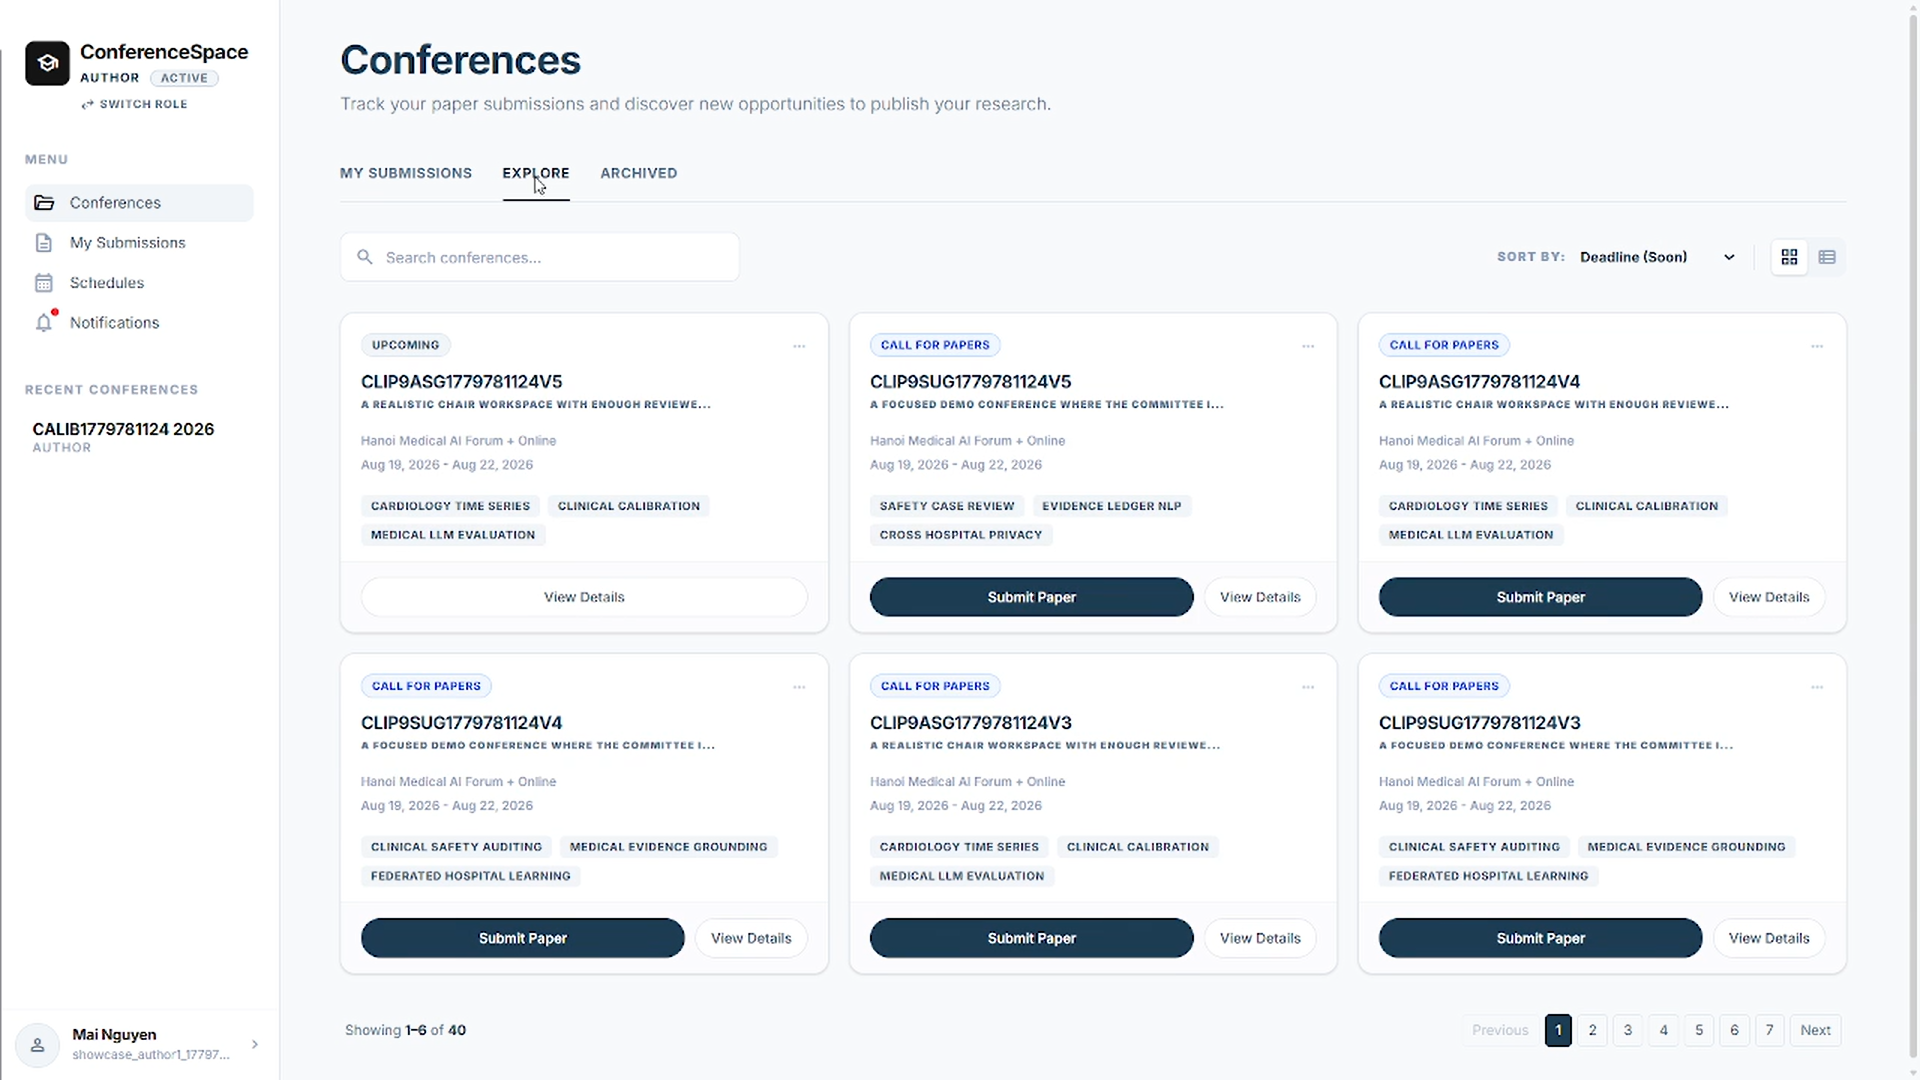
\includegraphics[width=0.95\textwidth]{images/chapter_3_uc01_explore_conferences.png}
  \caption{Giao diện khám phá danh sách hội nghị mặc định}
  \label{fig:uc01-explore-cut}
\end{figure}

Hình~\ref{fig:uc01-explore-cut} minh họa giao diện danh sách hội nghị mặc định mà Tác giả nhìn thấy khi bắt đầu tìm kiếm.

\begin{figure}[H]
  \centering
  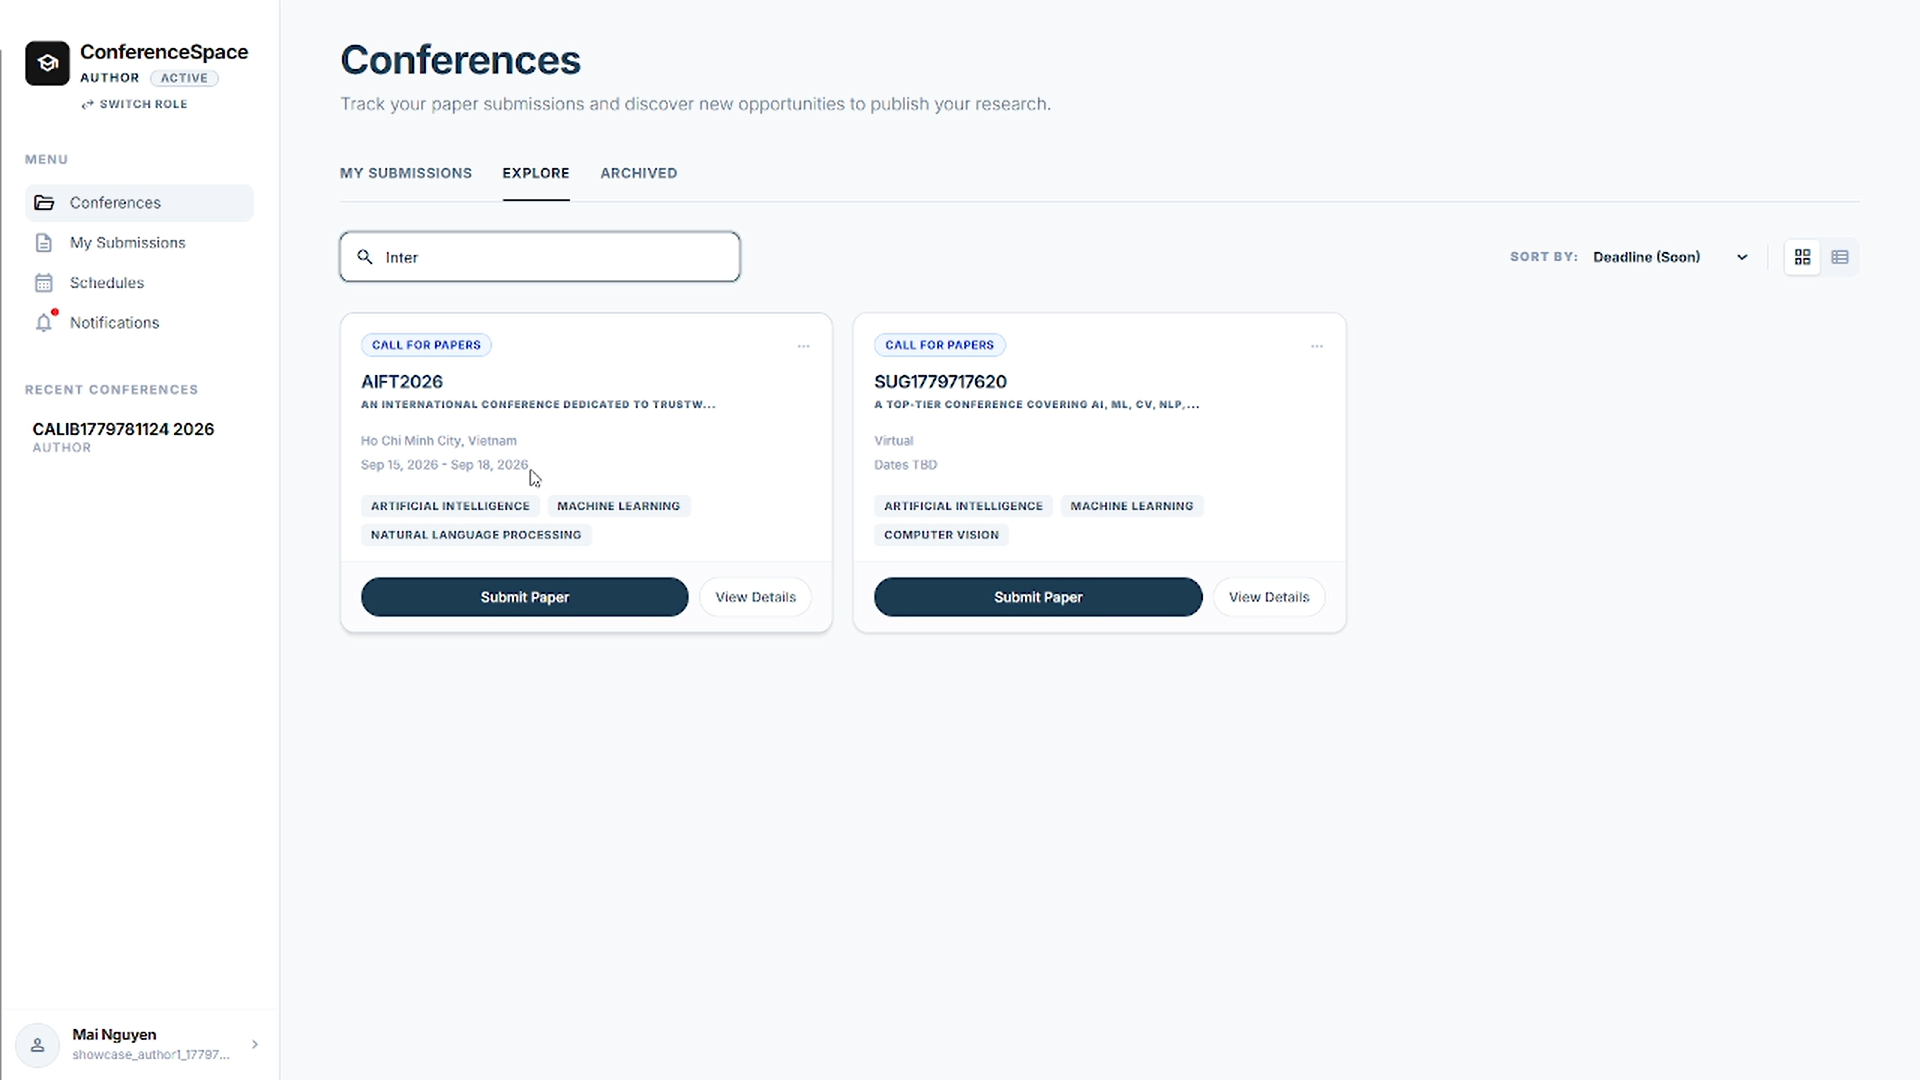
\includegraphics[width=0.95\textwidth]{images/chapter_3_uc01_search_conferences.png}
  \caption{Kết quả tìm kiếm và áp dụng bộ lọc động}
  \label{fig:uc01-search-cut}
\end{figure}

Hình~\ref{fig:uc01-search-cut} minh họa kết quả tìm kiếm sau khi Tác giả áp dụng bộ lọc động.

\begin{figure}[H]
  \centering
  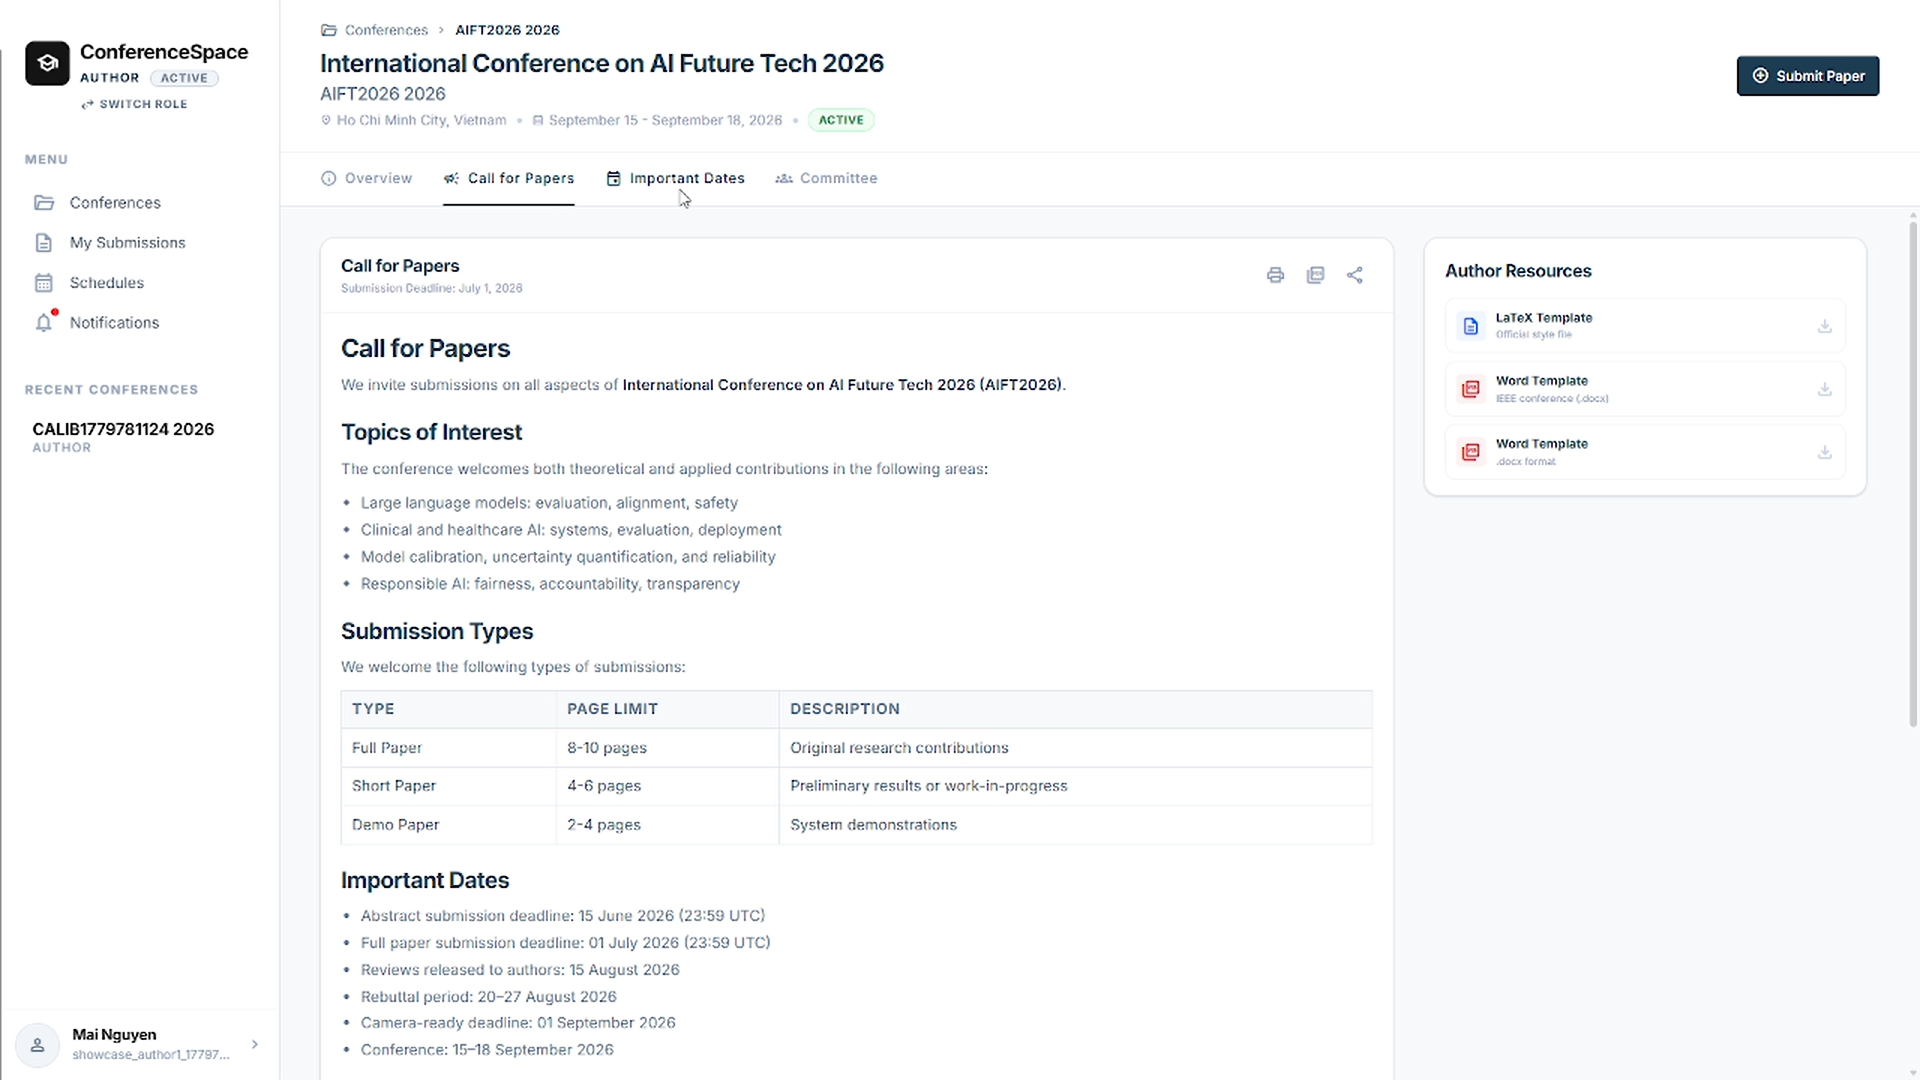
\includegraphics[width=0.95\textwidth]{images/chapter_3_uc01_conference_detail_cfp.png}
  \caption{Giao diện trang chi tiết hội nghị: Tab kêu gọi nộp bài (Call for Papers)}
  \label{fig:uc01-detail-cfp-cut}
\end{figure}

Hình~\ref{fig:uc01-detail-cfp-cut} thể hiện tab kêu gọi nộp bài (Call for Papers) trên trang chi tiết hội nghị.

\begin{figure}[H]
  \centering
  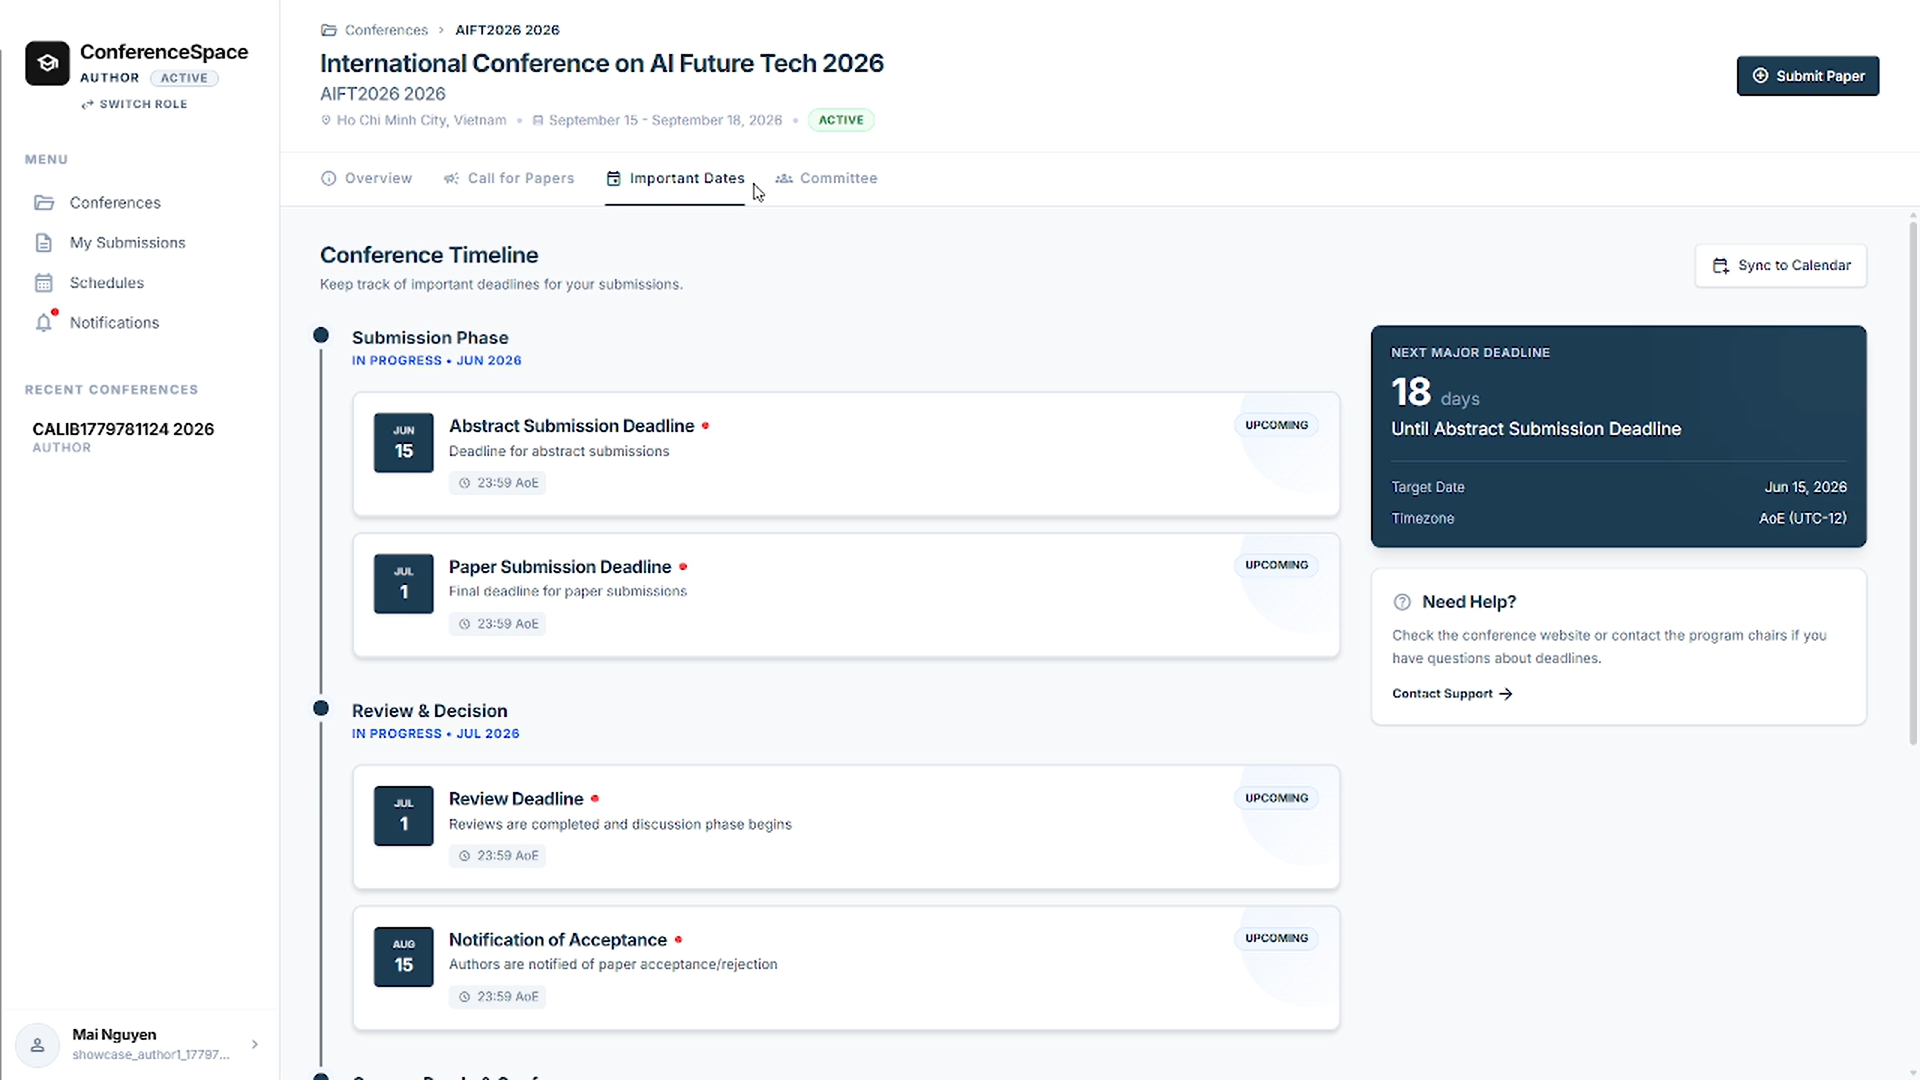
\includegraphics[width=0.95\textwidth]{images/chapter_3_uc01_conference_detail_dates.png}
  \caption{Giao diện trang chi tiết hội nghị: Tab mốc thời gian quan trọng (Important Dates)}
  \label{fig:uc01-detail-dates-cut}
\end{figure}


Hình~\ref{fig:uc01-detail-dates-cut} thể hiện tab mốc thời gian quan trọng trên trang chi tiết hội nghị.

\begin{figure}[H]
  \centering
  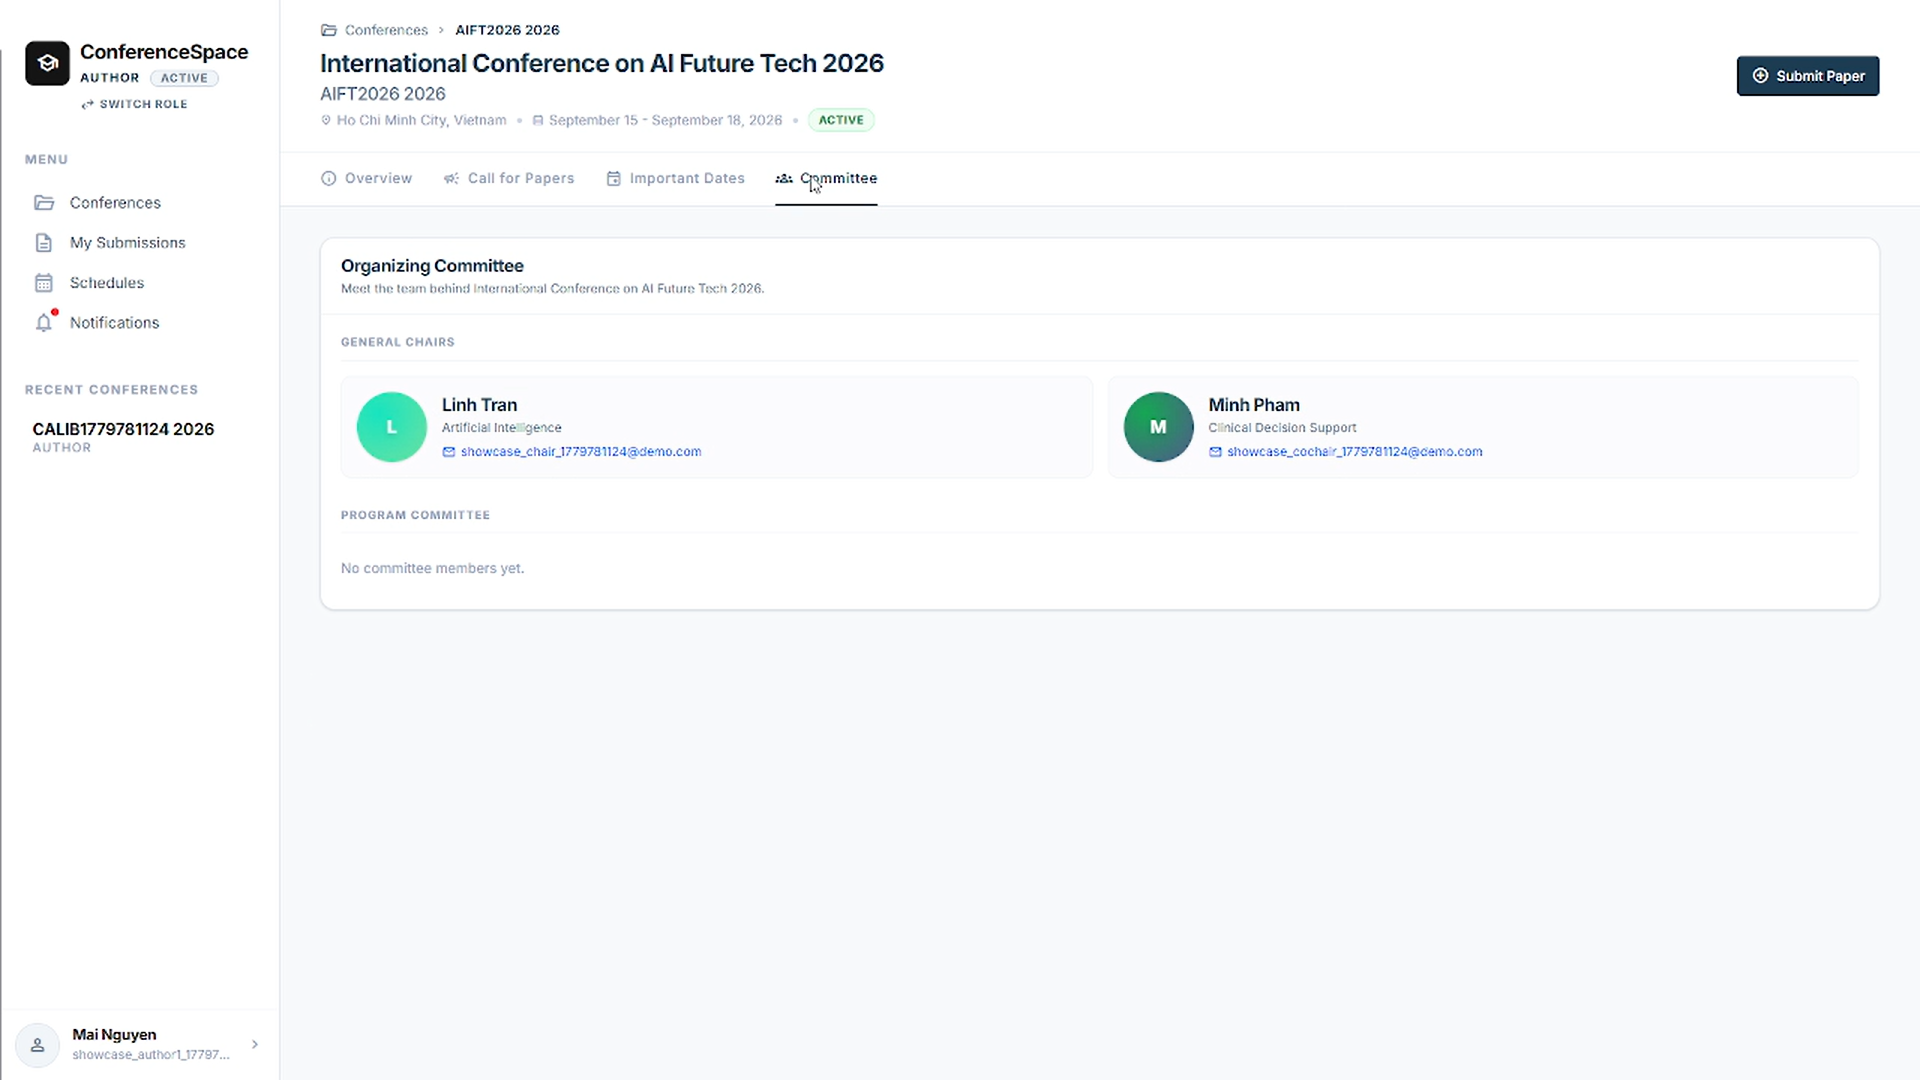
\includegraphics[width=0.95\textwidth]{images/chapter_3_uc01_conference_detail_committee.png}
  \caption{Giao diện trang chi tiết hội nghị: tab hội đồng chương trình (Committee)}
  \label{fig:uc01-detail-committee-cut}
\end{figure}

Hình~\ref{fig:uc01-detail-committee-cut} thể hiện tab hội đồng chương trình trên trang chi tiết hội nghị.

\begin{figure}[H]
  \centering
  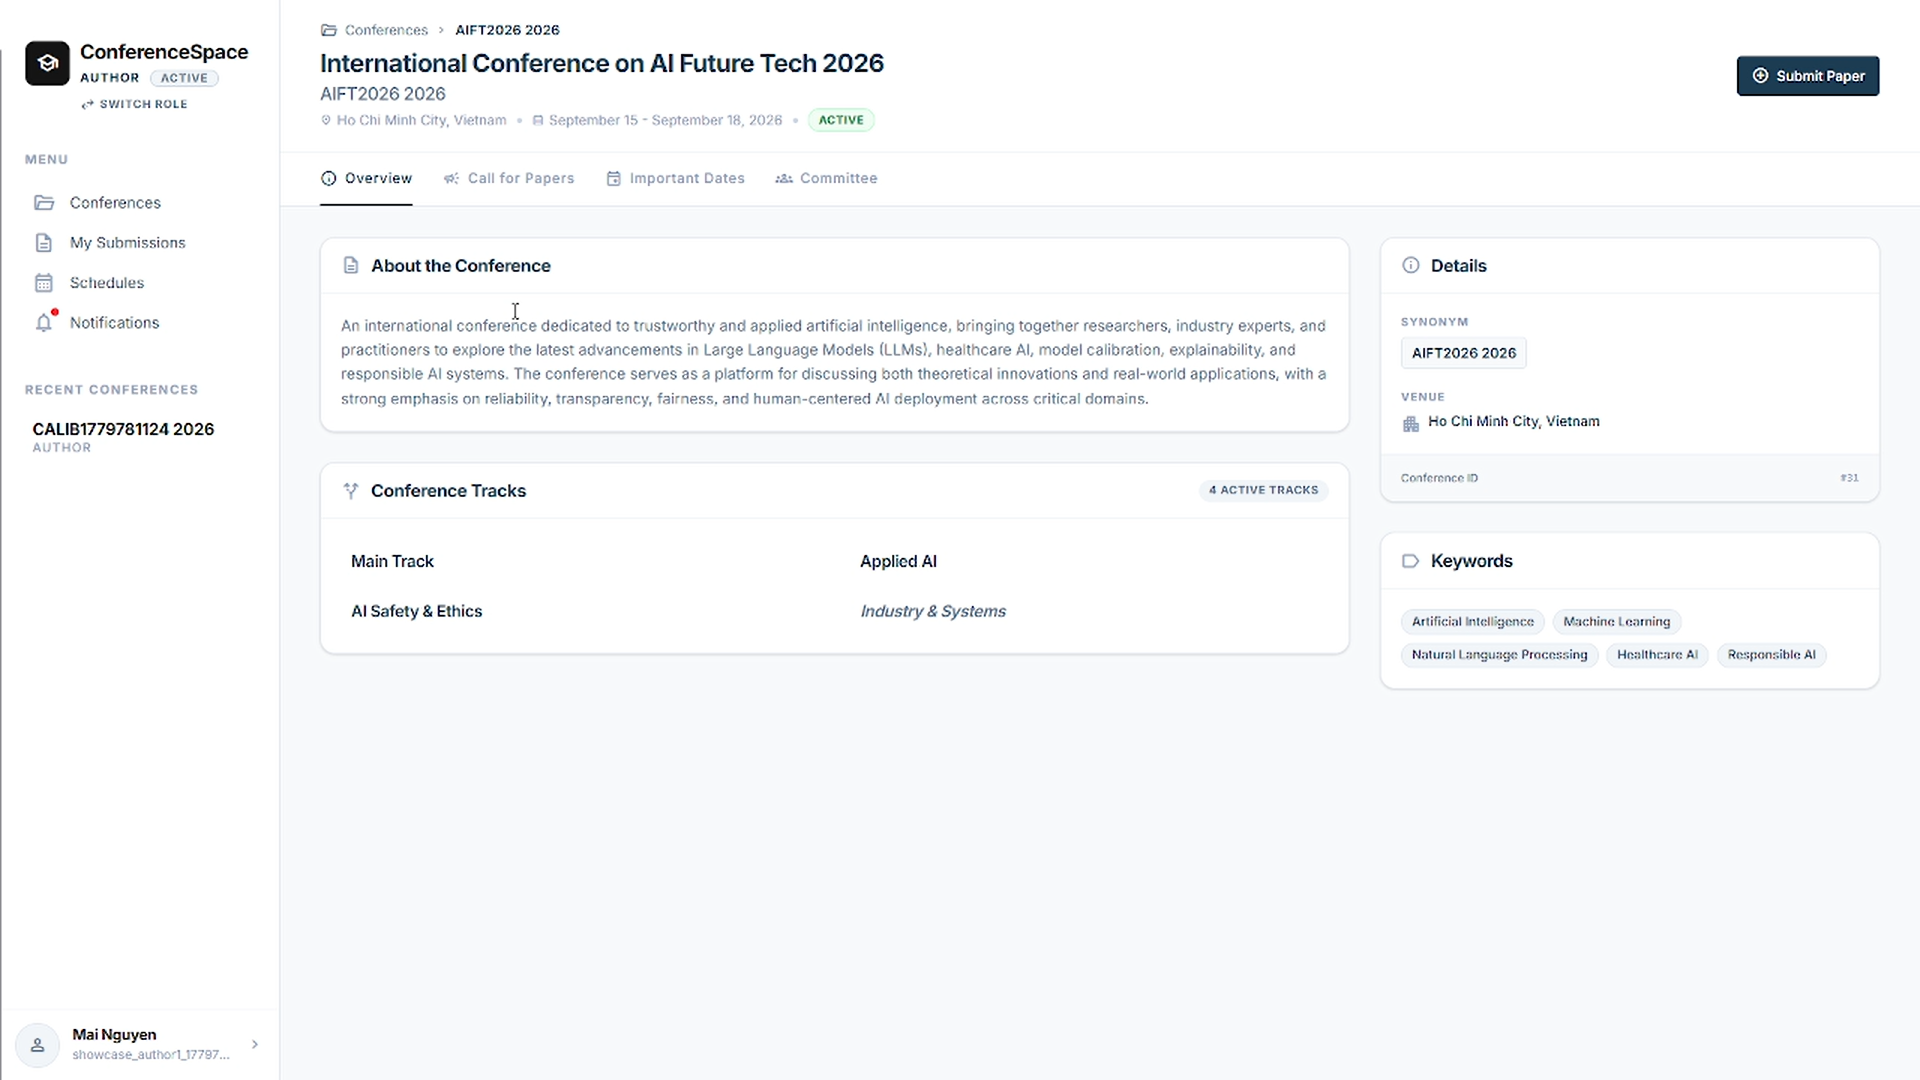
\includegraphics[width=0.95\textwidth]{images/chapter_3_uc01_conference_detail_overview.png}
  \caption{Giao diện trang chi tiết hội nghị: Tab tổng quan (Overview)}
  \label{fig:uc01-detail-overview-cut}
\end{figure}

Hình~\ref{fig:uc01-detail-overview-cut} thể hiện tab tổng quan của trang chi tiết hội nghị mà Tác giả xem trước khi quyết định nộp bài hoặc lưu theo dõi.

\subsubsection{UC-02. Hoàn tất và kiểm tra bài nộp}

Tác giả tạo bản nháp, tải bản thảo và có thể yêu cầu Submission Autofill trích xuất siêu dữ liệu cùng gợi ý chuyên đề trong danh sách hợp lệ. Tác giả kiểm tra, chỉnh sửa thông tin, khai báo đồng tác giả và xung đột lợi ích trước khi Submission Gating kiểm tra tệp, chính sách và các điều kiện gửi bài. Trạng thái \textit{warn} cho phép tiếp tục khi chính sách hội nghị cho phép; trạng thái \textit{block} ngăn gửi cho đến khi lỗi có căn cứ được khắc phục. Nếu Submission Autofill không khả dụng, Tác giả vẫn có thể nhập và lưu bản nháp thủ công. Nếu Submission Gating không trả được bất kỳ kết quả hợp lệ nào, backend chưa cho phép gửi bài cho đến khi thực hiện được một lần kiểm tra hợp lệ.

\begin{figure}[H]
  \centering
  \begin{minipage}{0.48\textwidth}
    \centering
    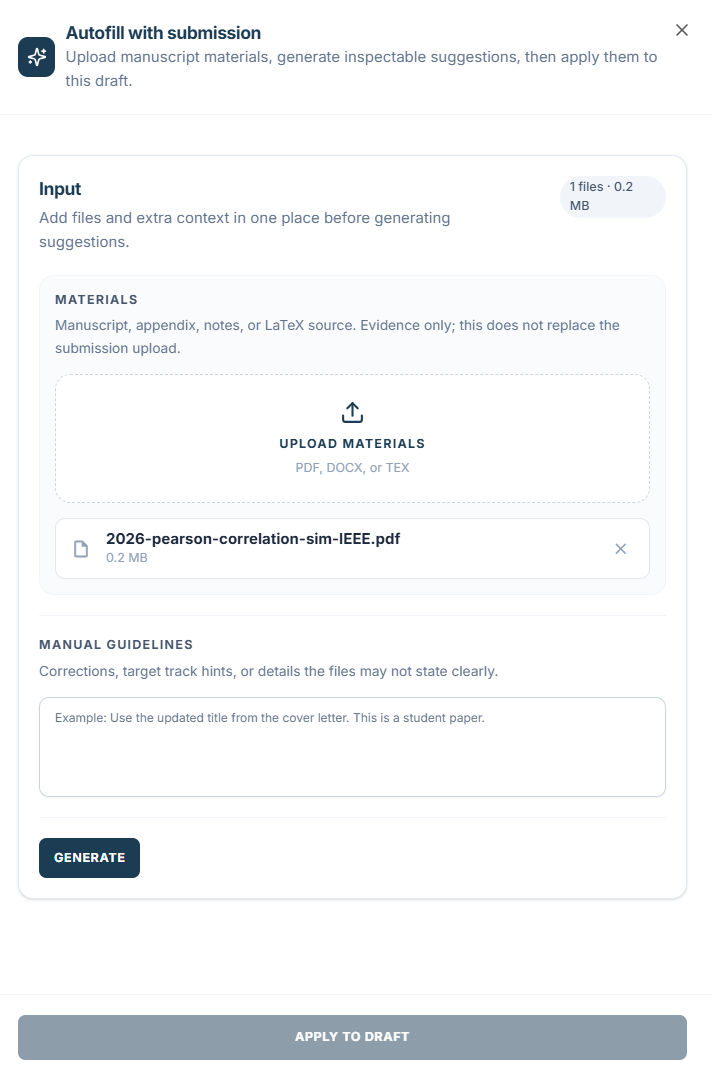
\includegraphics[width=0.56\textwidth]{images/chapter_3_uc02_autofill_1.png}
  \end{minipage}
  \begin{minipage}{0.48\textwidth}
    \centering
    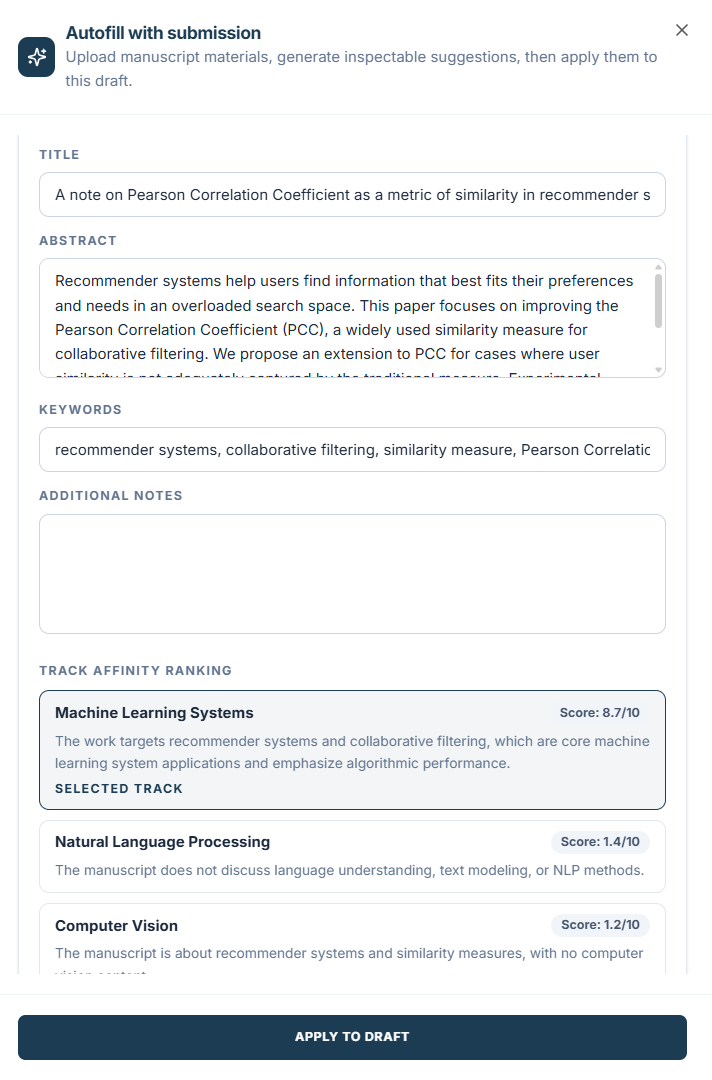
\includegraphics[width=0.56\textwidth]{images/chapter_3_uc02_autofill_2.png}
  \end{minipage}
  \caption{Giao diện tải lên bản thảo (trái) và kết quả trích xuất thông tin tự động (phải)}
  \label{fig:uc02-autofill-cut}
\end{figure}

Hình~\ref{fig:uc02-autofill-cut} trình bày giao diện tải lên bản thảo (trái) cùng kết quả trích xuất thông tin mà Submission Autofill trả về (phải) để Tác giả kiểm tra và chỉnh sửa.

\begin{figure}[H]
  \centering
  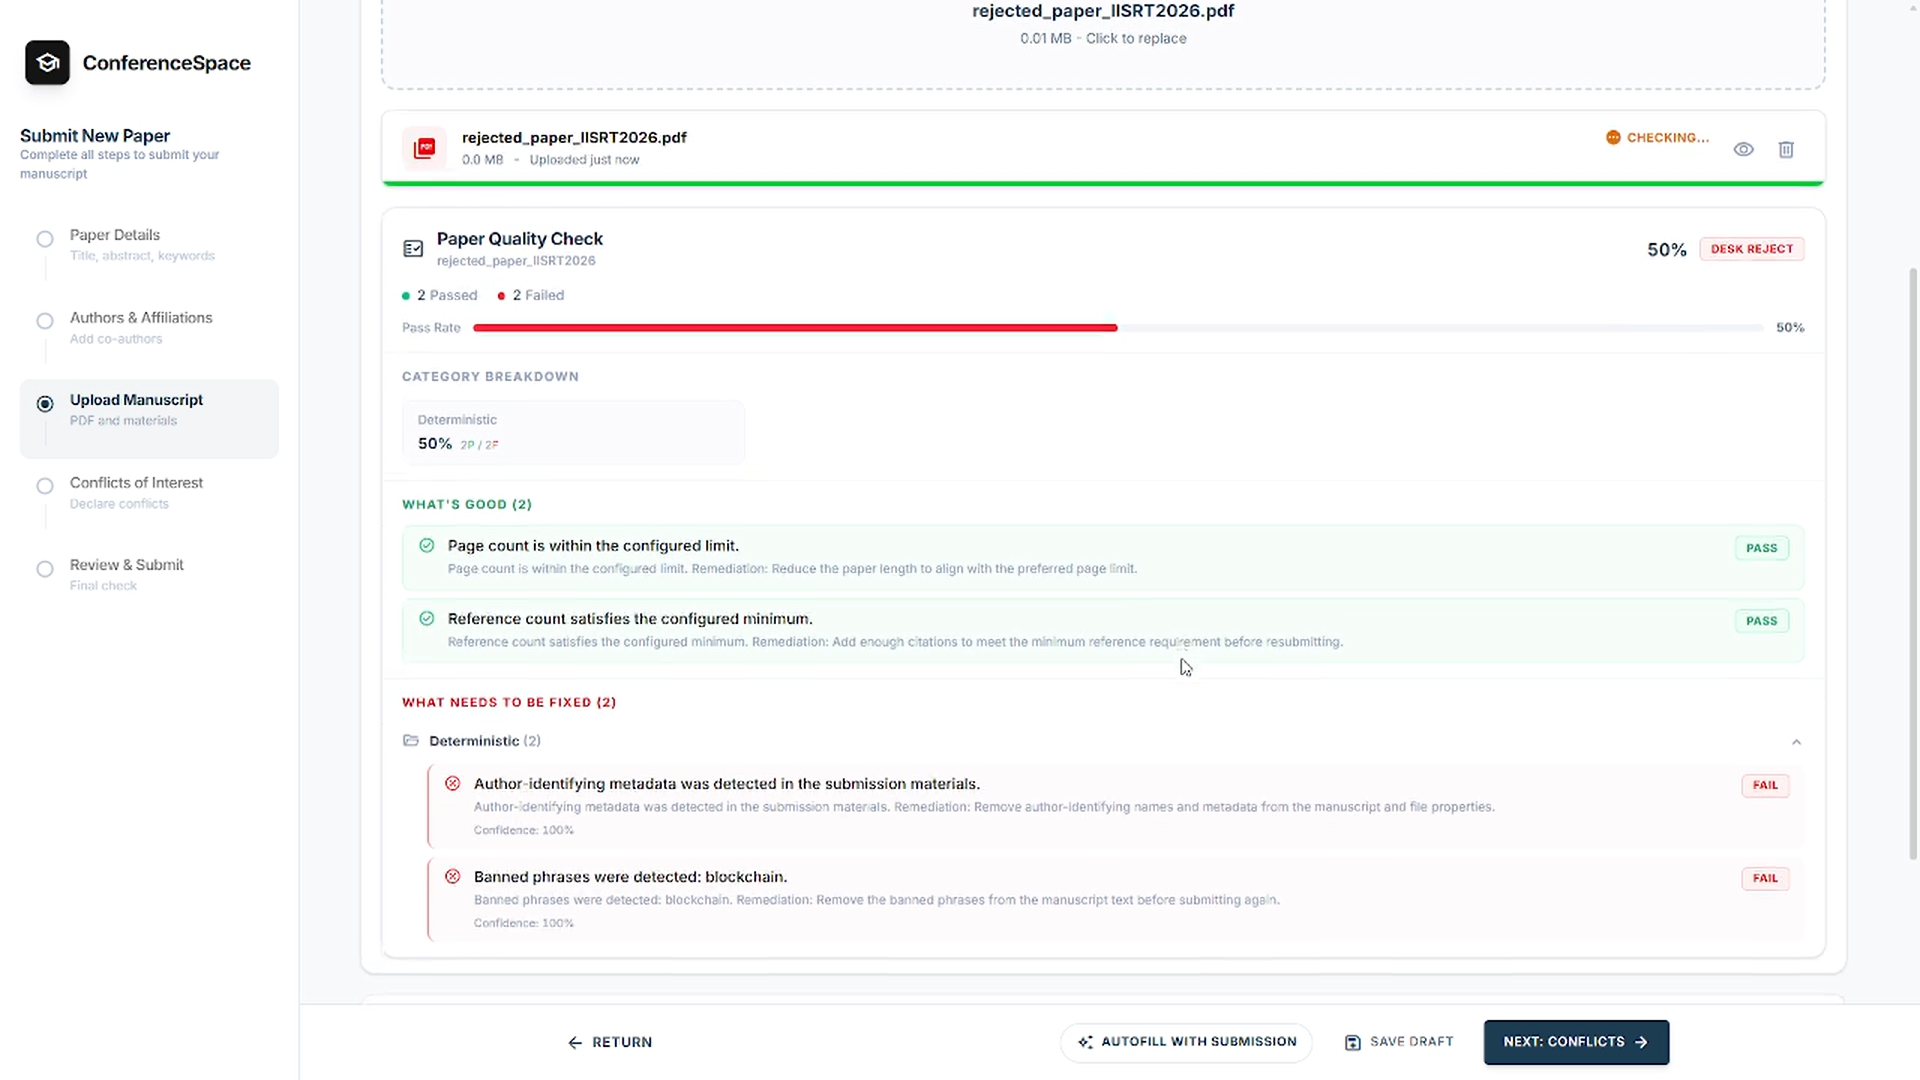
\includegraphics[width=0.95\textwidth]{images/chapter_3_uc02_precheck_gating.png}
  \caption{Kết quả Submission Gating theo ba trạng thái \textit{pass}, \textit{warn} và \textit{block}}
  \label{fig:uc02-gating-cut}
\end{figure}

Trước khi gửi bài, Tác giả xem kết quả kiểm tra tự động của Submission Gating tại Hình~\ref{fig:uc02-gating-cut}, gồm ba trạng thái \textit{pass}, \textit{warn} và \textit{block}.

\begin{figure}[H]
  \centering
  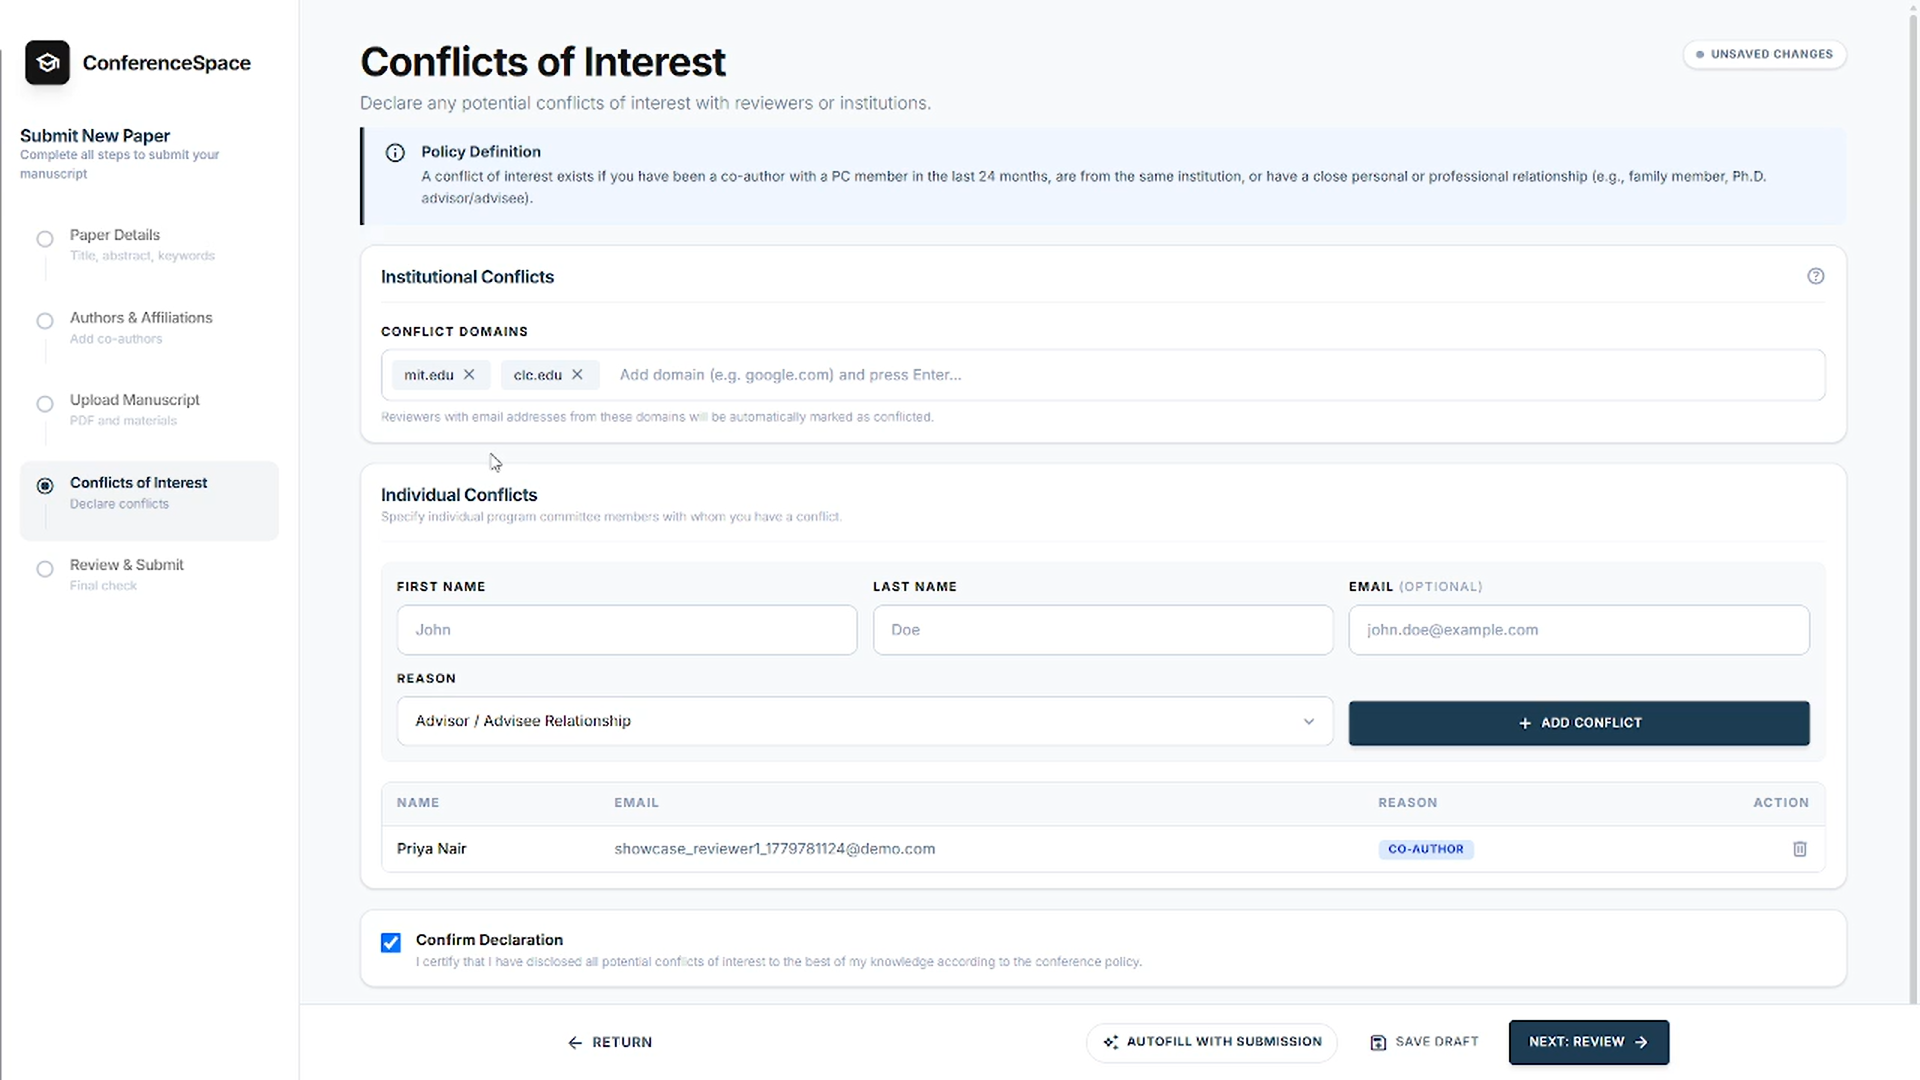
\includegraphics[width=0.95\textwidth]{images/chapter_3_uc02_authors_conflict.png}
  \caption{Giao diện khai báo thông tin các đồng tác giả và xung đột lợi ích}
  \label{fig:uc02-authors-conflict-cut}
\end{figure}

Hình~\ref{fig:uc02-authors-conflict-cut} minh họa giao diện khai báo đồng tác giả và xung đột lợi ích mà Tác giả hoàn tất trước khi Submission Gating kiểm tra.

Hai chức năng AI chỉ hỗ trợ hoàn tất bài nộp: Submission Autofill tạo bản nháp có thể sửa, còn Submission Gating kiểm tra điều kiện trước khi gửi. Tác giả vẫn là người xác nhận dữ liệu và thực hiện thao tác gửi chính thức.

\subsubsection{UC-03. Quản lý vòng đời bài nộp}

Sau khi tạo bài, Tác giả theo dõi và thực hiện các hành động phù hợp với từng trạng thái: chỉnh sửa bản nháp; theo dõi hoặc rút bài đã gửi khi cấu hình và hạn chót nộp bài cho phép; xem phản biện khi được công bố; gửi phản hồi trong giai đoạn do Chủ tọa hoặc Đồng chủ tọa mở; và tải bản thảo hoàn chỉnh khi bài được chấp nhận. Backend từ chối yêu cầu không phù hợp với trạng thái hoặc hạn chót tương ứng. Phiên bản hiện tại hỗ trợ tải và truy xuất bản thảo hoàn chỉnh nhưng chưa có luồng để Chủ tọa phê duyệt, yêu cầu nộp lại hoặc kiểm tra hạn chót nộp bản thảo hoàn chỉnh tại thời điểm thực thi.

\begin{figure}[H]
  \centering
  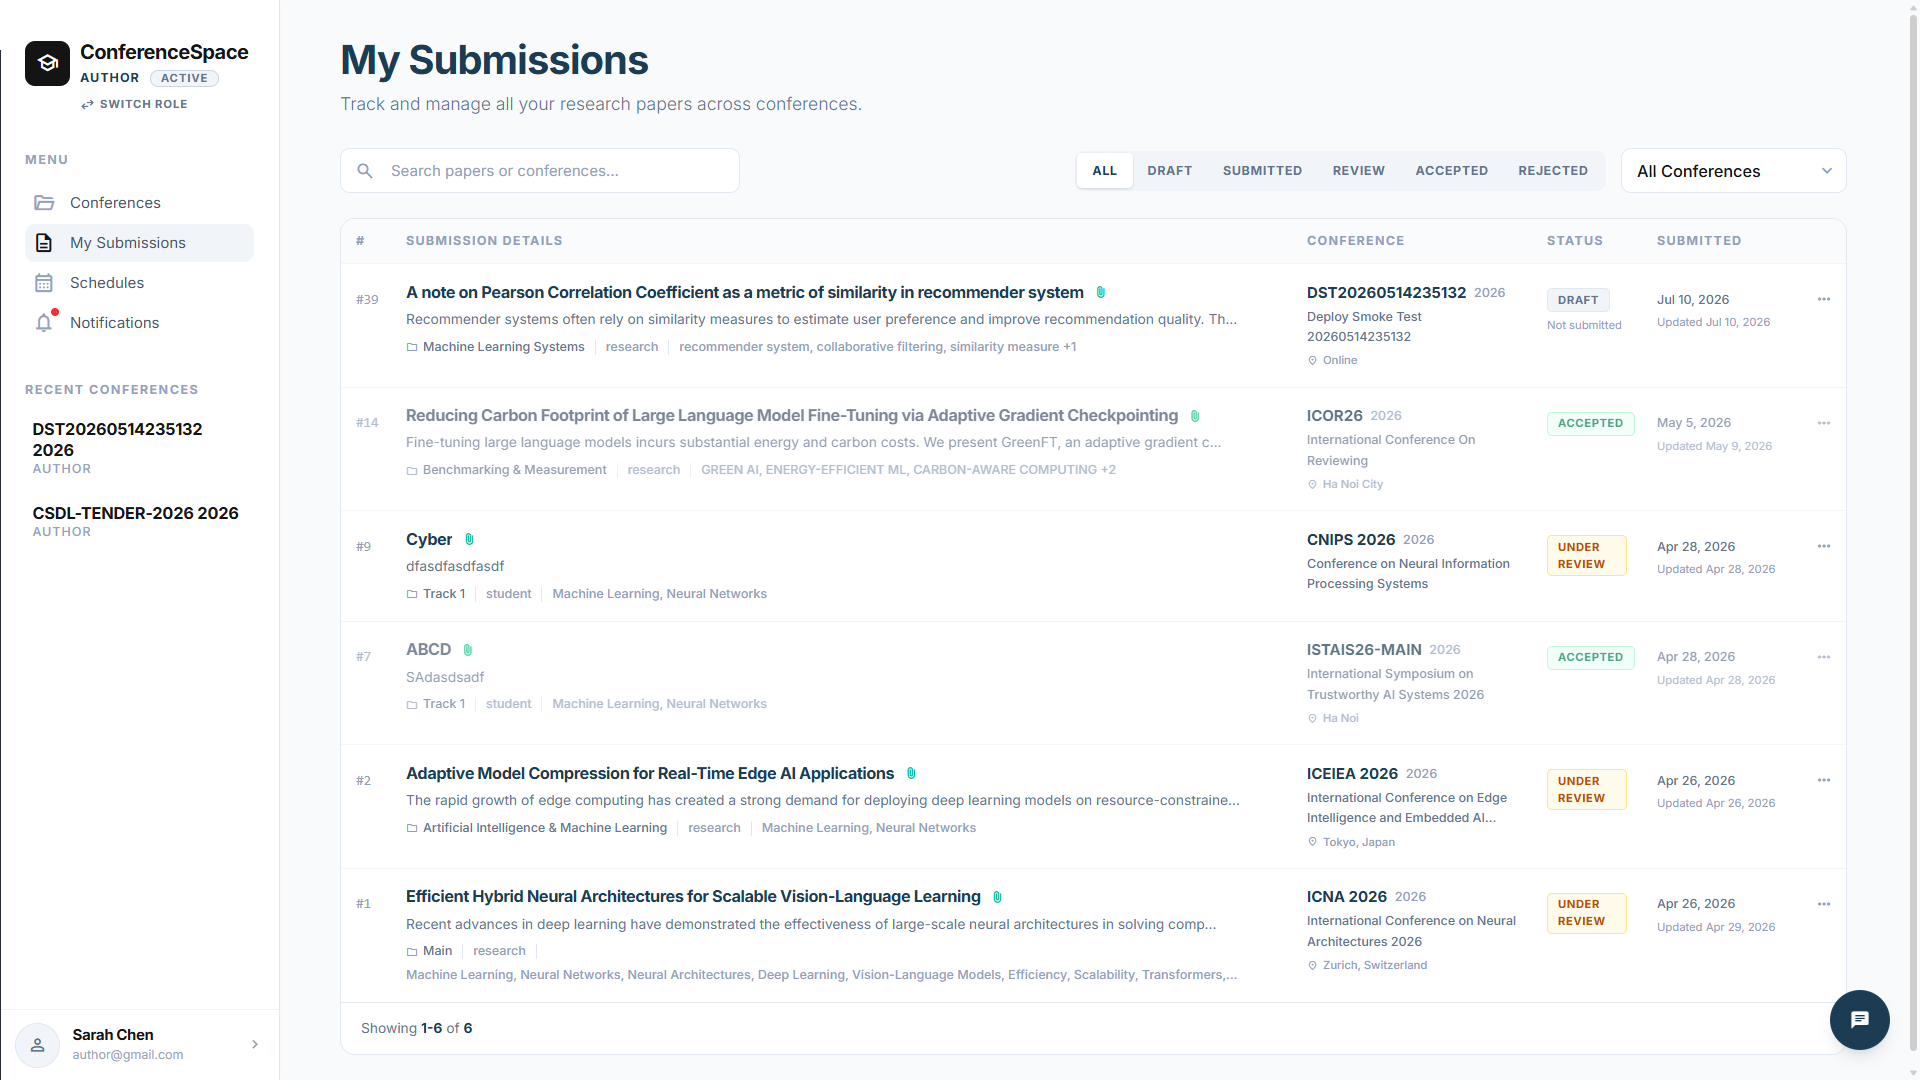
\includegraphics[width=0.95\textwidth]{images/chapter_3_uc03_submissions_list.png}
  \caption{Danh sách bài nộp và trạng thái vòng đời trong không gian làm việc của Tác giả}
  \label{fig:uc03-submissions-cut}
\end{figure}

Giao diện ở Hình~\ref{fig:uc03-submissions-cut} cung cấp một điểm nhìn thống nhất để Tác giả nhận biết trạng thái hiện hành và thao tác nghiệp vụ còn hợp lệ, thay vì chỉ minh họa riêng các chức năng AI ở bước chuẩn bị bài.

\begin{figure}[H]
  \centering
  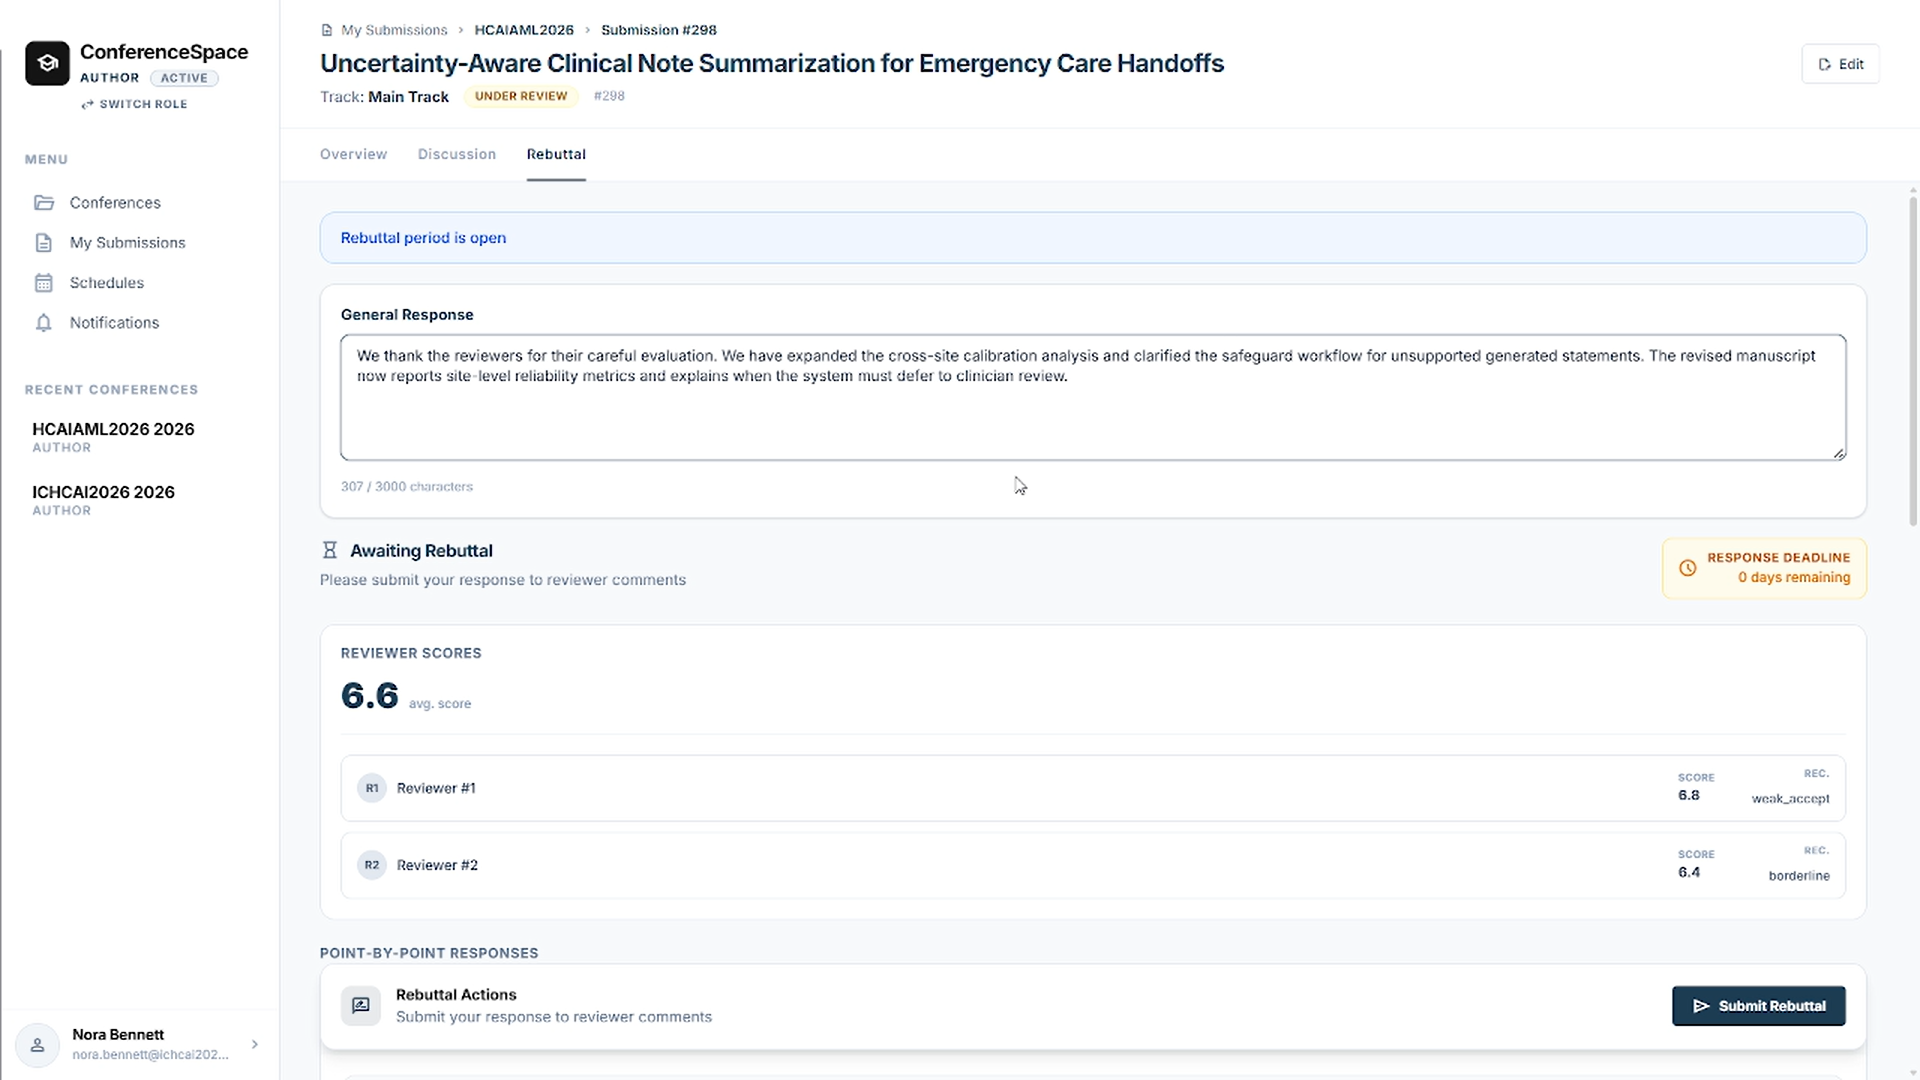
\includegraphics[width=0.95\textwidth]{images/chapter_3_uc03_rebuttal.png}
  \caption{Giao diện soạn thảo và gửi phản hồi của tác giả (rebuttal)}
  \label{fig:uc03-rebuttal-cut}
\end{figure}

Hình~\ref{fig:uc03-rebuttal-cut} minh họa giao diện Tác giả soạn và gửi phản hồi (rebuttal) trong giai đoạn phản hồi.

\begin{figure}[H]
  \centering
  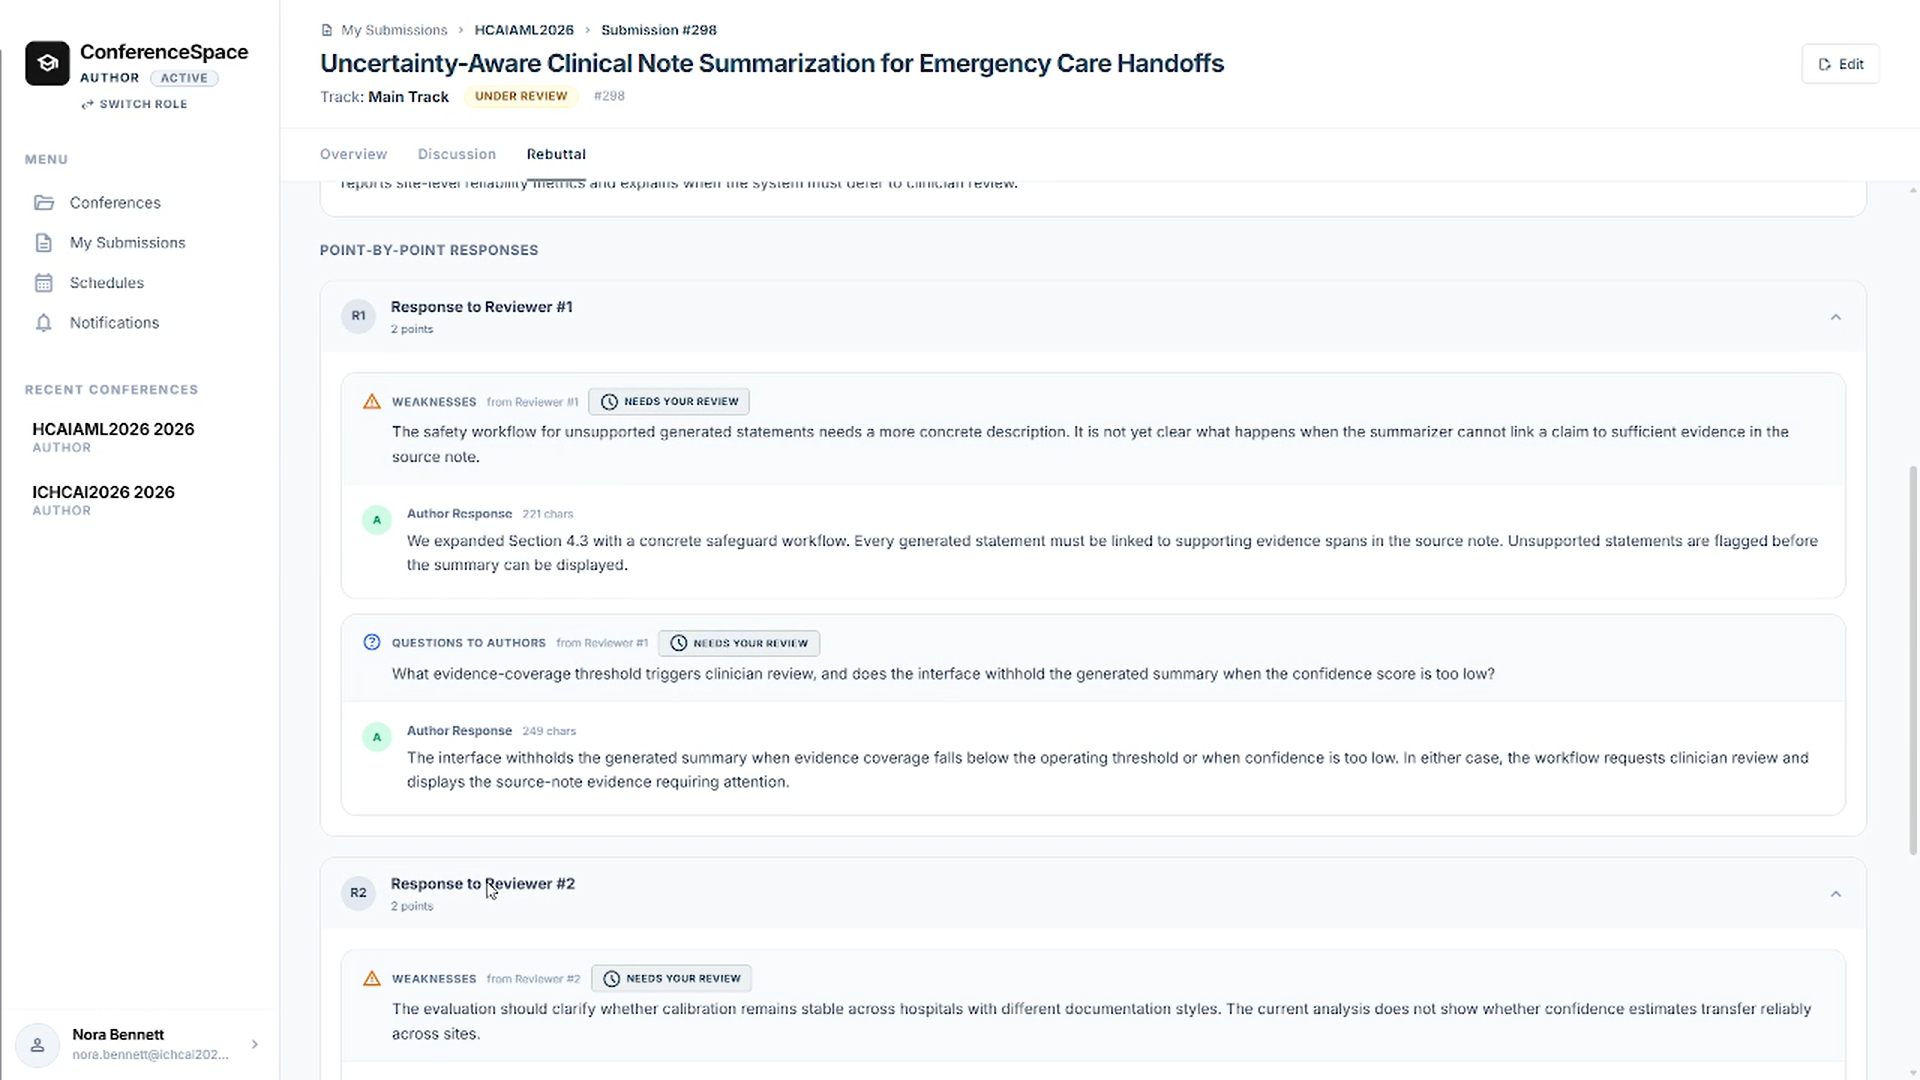
\includegraphics[width=0.95\textwidth]{images/chapter_3_uc03_rebuttal_2.png}
  \caption{Biến thể giao diện soạn và gửi phản hồi của Tác giả (rebuttal)}
  \label{fig:uc03-rebuttal-2-cut}
\end{figure}

Hình~\ref{fig:uc03-rebuttal-2-cut} trình bày một biến thể khác của giao diện soạn thảo và gửi phản hồi.

\begin{figure}[H]
  \centering
  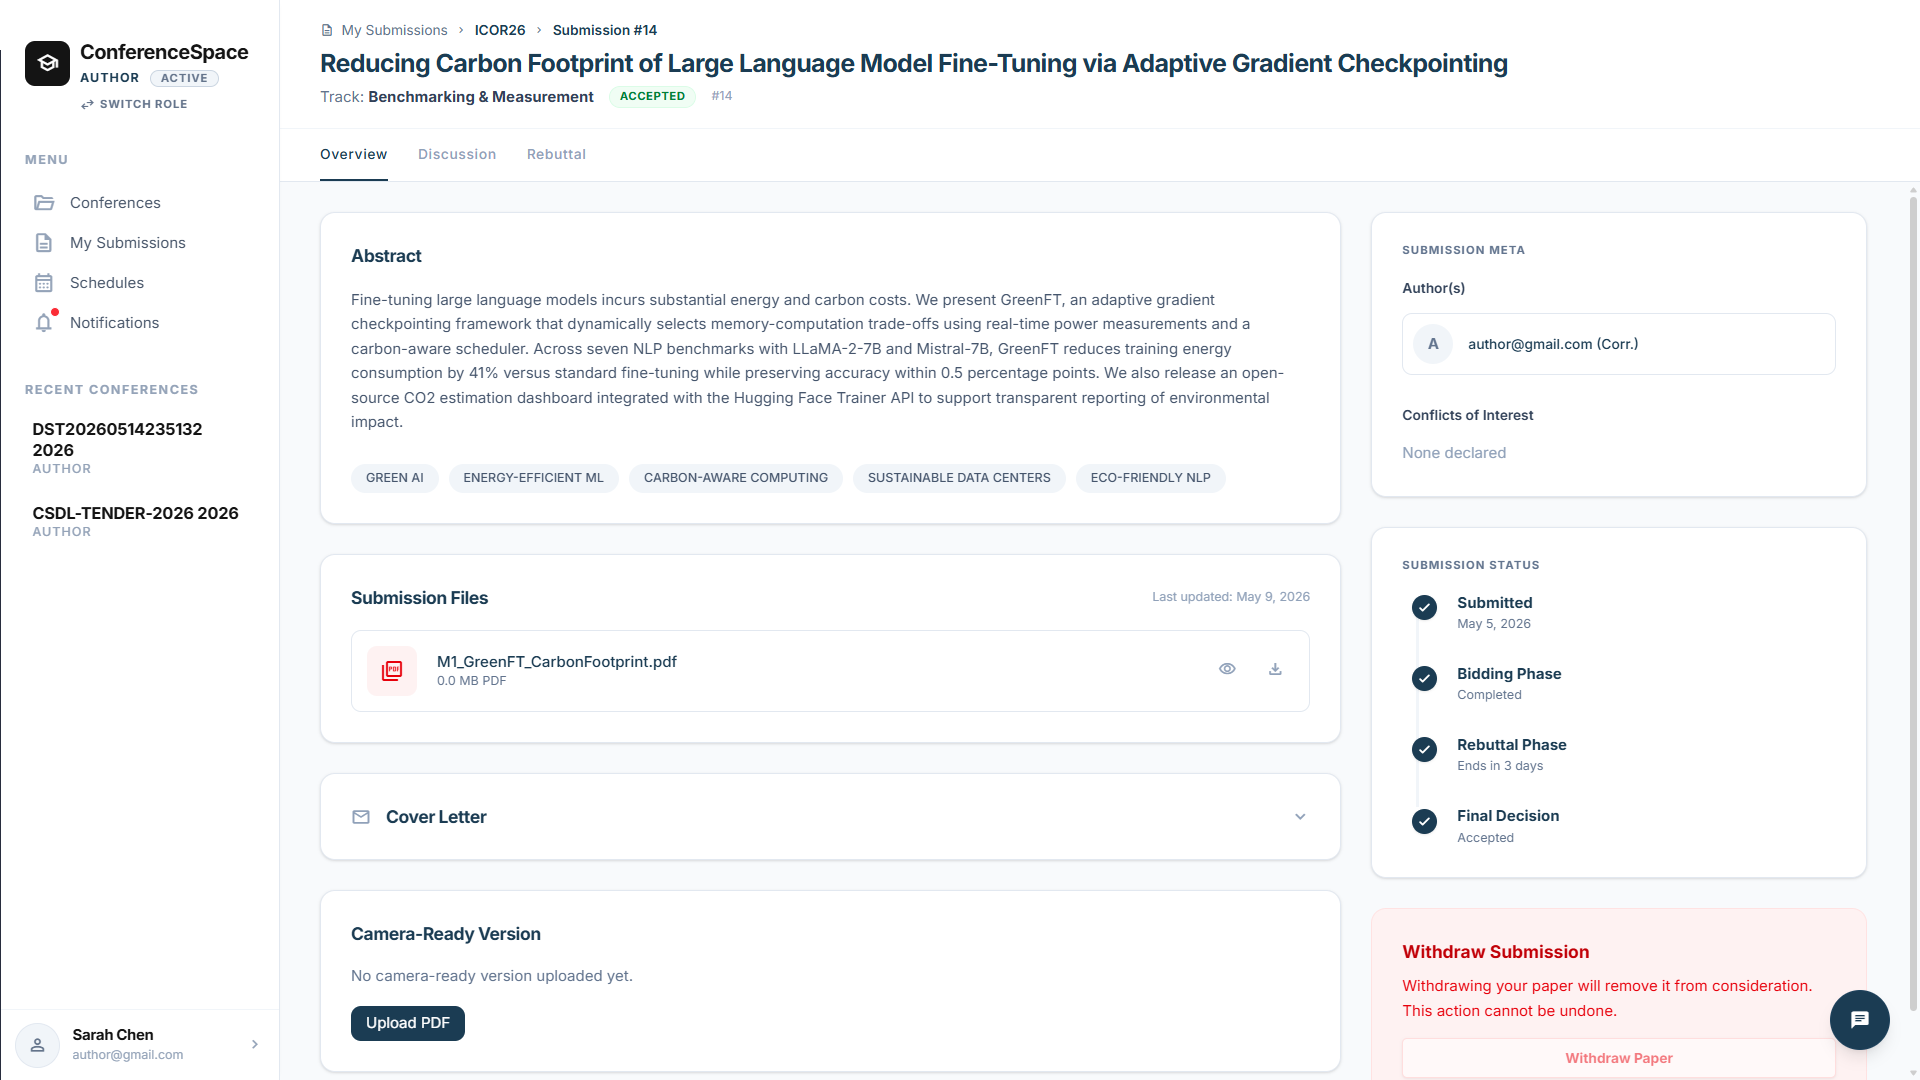
\includegraphics[width=0.95\textwidth]{images/chapter_3_uc03_submission_detail.png}
  \caption{Giao diện trang chi tiết bài nộp, xem nhận định chuyên môn và tải bản thảo hoàn chỉnh (camera-ready)}
  \label{fig:uc03-submission-detail-cut}
\end{figure}

Hình~\ref{fig:uc03-submission-detail-cut} thể hiện trang chi tiết bài nộp, nơi Tác giả xem nhận định chuyên môn và tải lên bản chỉnh sửa cuối cùng khi bài được chấp nhận.

\subsubsection{UC-04. Tiếp nhận lời mời hội nghị và xem bài được phân công}

Chủ tọa gửi lời mời tham gia hội nghị; hệ thống lưu trạng thái và thông báo cho người nhận. Phản biện viên chỉ có thể chấp nhận hoặc từ chối lời mời của chính mình. Đây là trạng thái tham gia hội nghị của Phản biện viên, khác với trạng thái của từng phân công bài. Khi Chủ tọa đã tạo phân công, Phản biện viên xem bài, hạn chót nộp bài và trạng thái trên bảng điều khiển; backend chỉ trả các phân công thuộc người dùng hiện tại. Kho mã nguồn có thao tác phản hồi phân công theo định danh, nhưng luồng giao diện được mô tả trong chương này không đồng nhất thao tác đó với việc chấp nhận lời mời hội nghị.

\begin{figure}[H]
  \centering
  \begin{tabular}{c}
    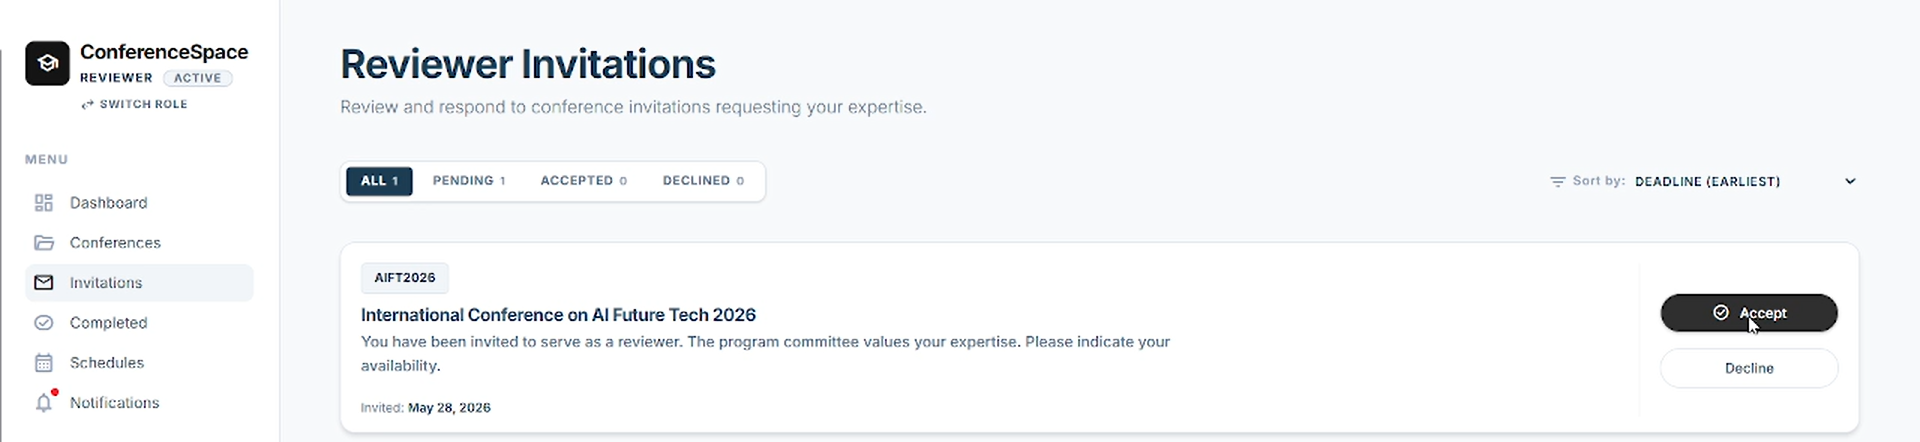
\includegraphics[width=0.95\textwidth]{images/chapter_3_uc04_reviewer_invitations_1.png} \\
    \vspace{0.2cm}
    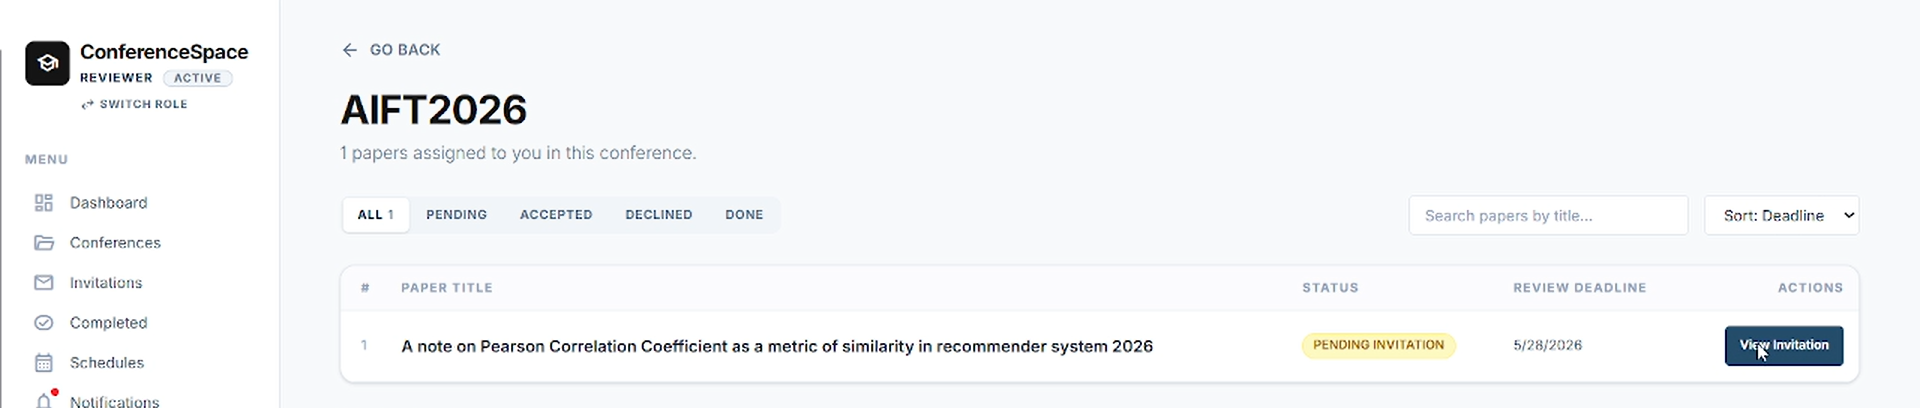
\includegraphics[width=0.95\textwidth]{images/chapter_3_uc04_reviewer_invitations_2.png}
  \end{tabular}
  \caption{Email thông báo lời mời (trên) và danh sách lời mời tham gia phản biện trong hệ thống (dưới)}
  \label{fig:uc04-invitations-cut}
\end{figure}

Hình~\ref{fig:uc04-invitations-cut} minh họa giao diện tiếp nhận thông báo và danh sách lời mời tham gia phản biện hội nghị.

\begin{figure}[H]
  \centering
  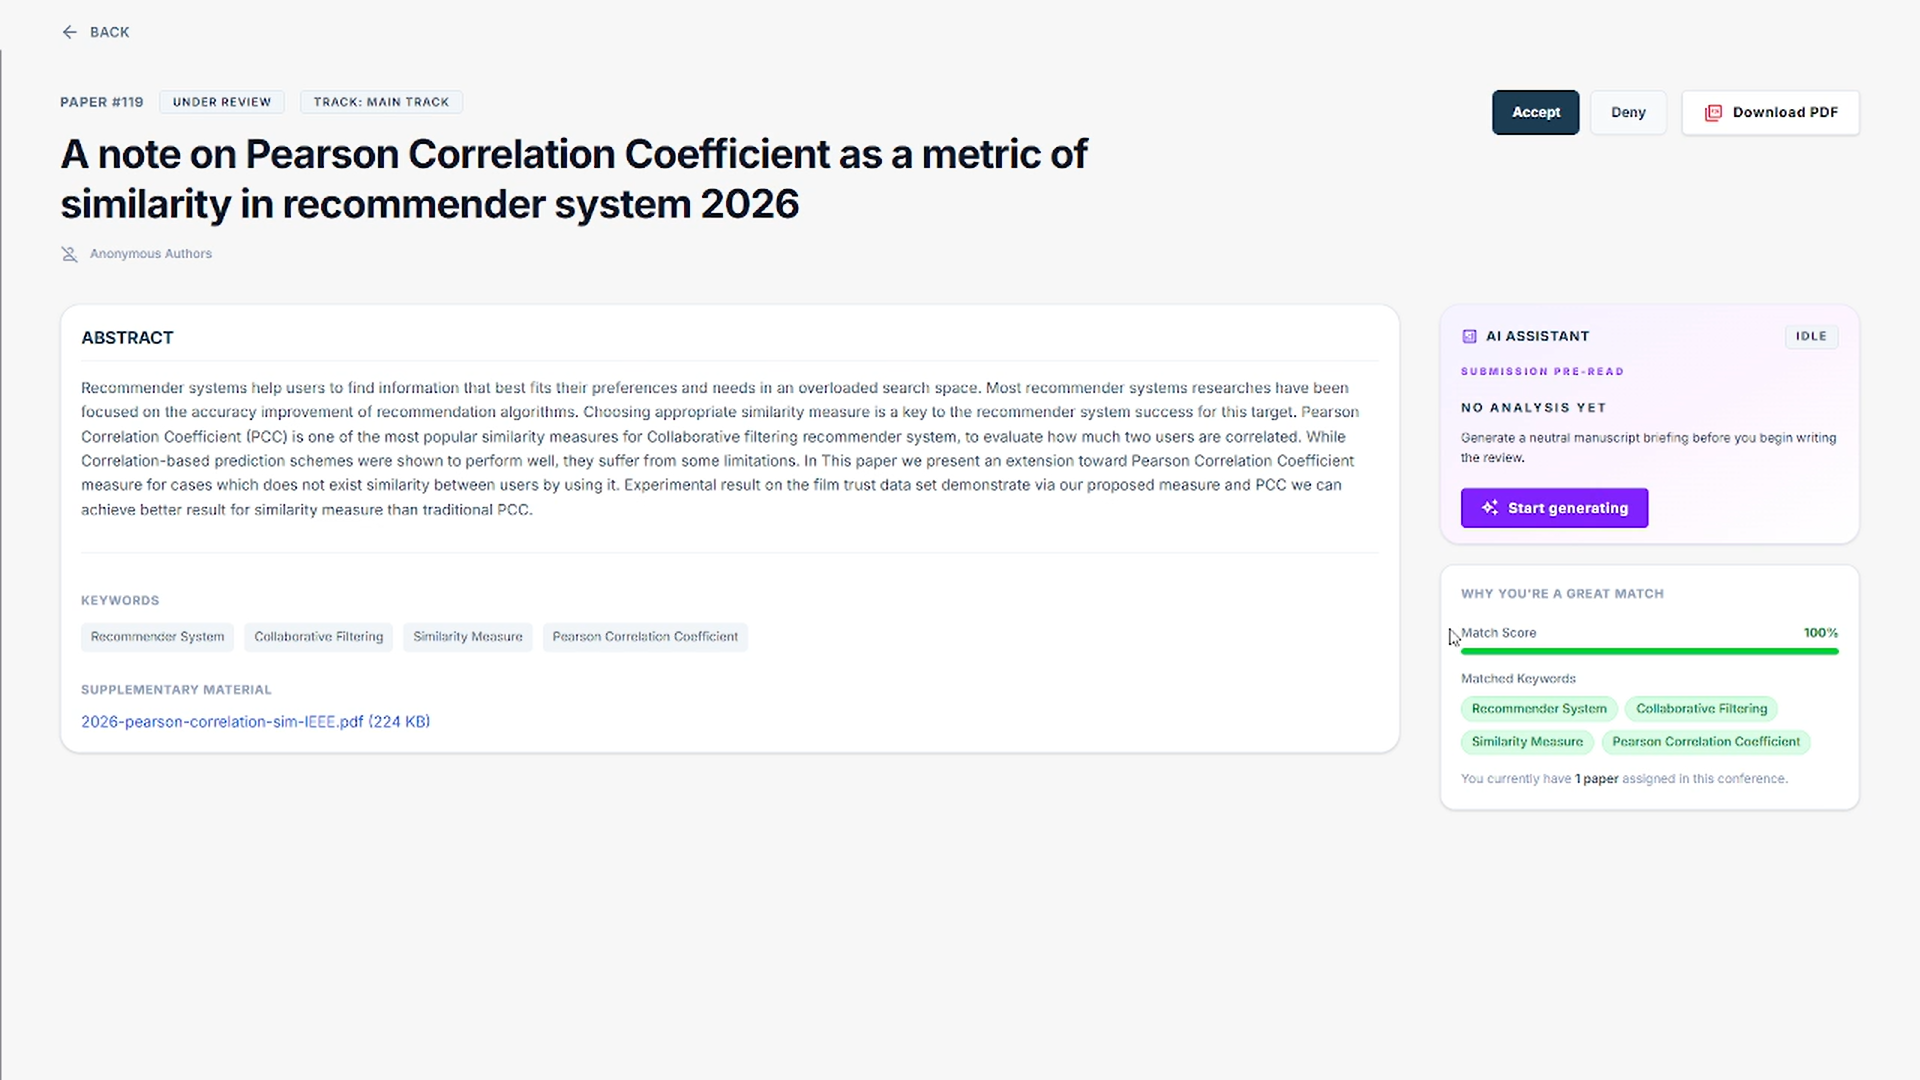
\includegraphics[width=0.95\textwidth]{images/chapter_3_uc04_accept_deny_assignment.png}
  \caption{Giao diện chi tiết bài nộp để Phản biện viên chấp nhận hoặc từ chối phân công}
  \label{fig:uc04-accept-deny-cut}
\end{figure}

Sau khi Chủ tọa tạo phân công, Phản biện viên dùng giao diện tại Hình~\ref{fig:uc04-accept-deny-cut} để xem bài nộp và chấp nhận hoặc từ chối phân công.

\subsubsection{UC-05. Đọc, soạn và gửi phản biện có AI hỗ trợ}

Phản biện viên mở bài được phân công, đọc bản thảo và nhập điểm, nhận xét, khuyến nghị cùng mức độ tự tin. Reviewer Initial Analysis có thể cung cấp bản định hướng ban đầu, nhưng Phản biện viên phải đối chiếu nội dung này với bài gốc và tự hình thành nhận định. Trước khi gửi, Review Quality Auditor rà soát mức độ đầy đủ, cụ thể và nhất quán của bản nháp. Phản biện viên xem các phát hiện, chỉnh sửa khi cần và xác nhận gửi phản biện.

\begin{figure}[H]
  \centering
  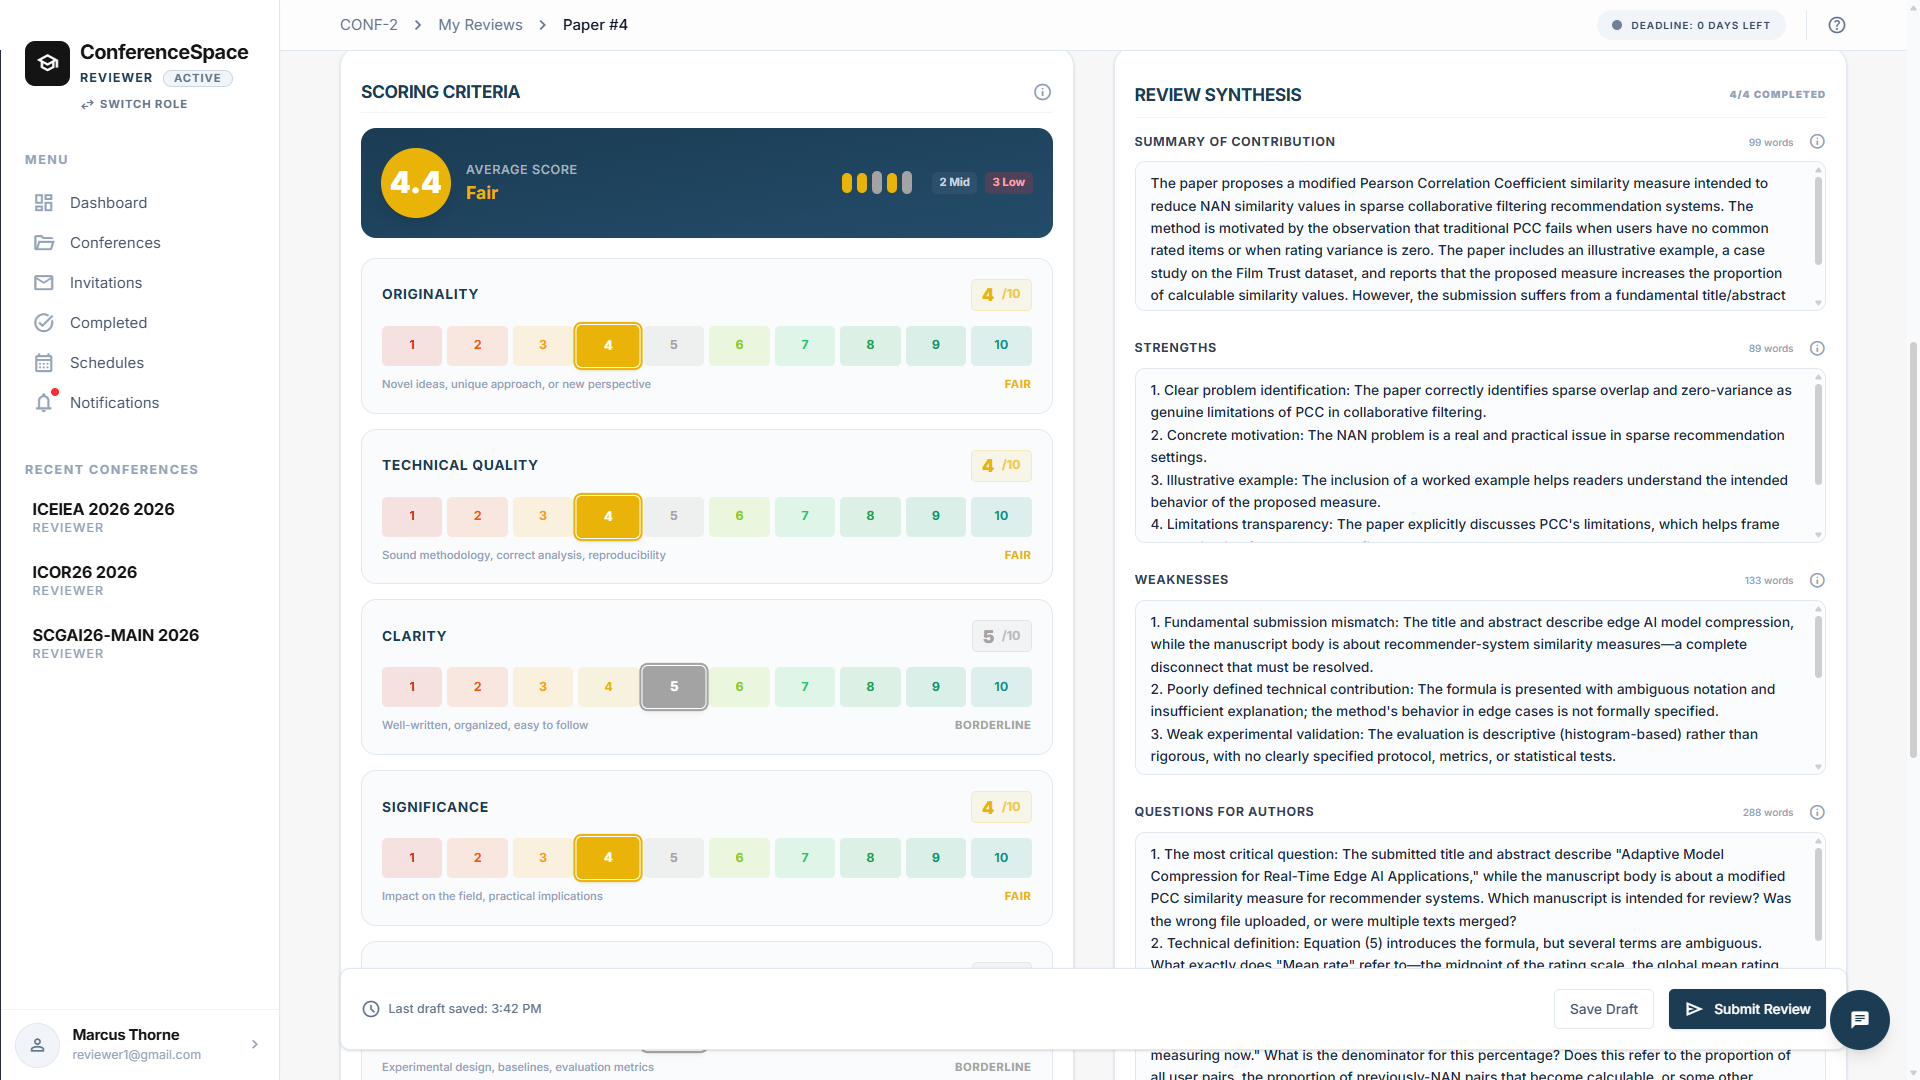
\includegraphics[width=0.95\textwidth]{images/chapter_3_uc05_reviewer_workspace_1.png}
  \caption{Không gian đọc bài và soạn phản biện của Phản biện viên}
  \label{fig:uc05-workspace-cut}
\end{figure}

Hình~\ref{fig:uc05-workspace-cut} đặt hai chức năng AI vào đúng bối cảnh sử dụng: chúng hỗ trợ một quy trình mà Phản biện viên vẫn phải đọc bản thảo, nhập nhận xét và chịu trách nhiệm về bản phản biện cuối cùng.

\begin{figure}[H]
  \centering
  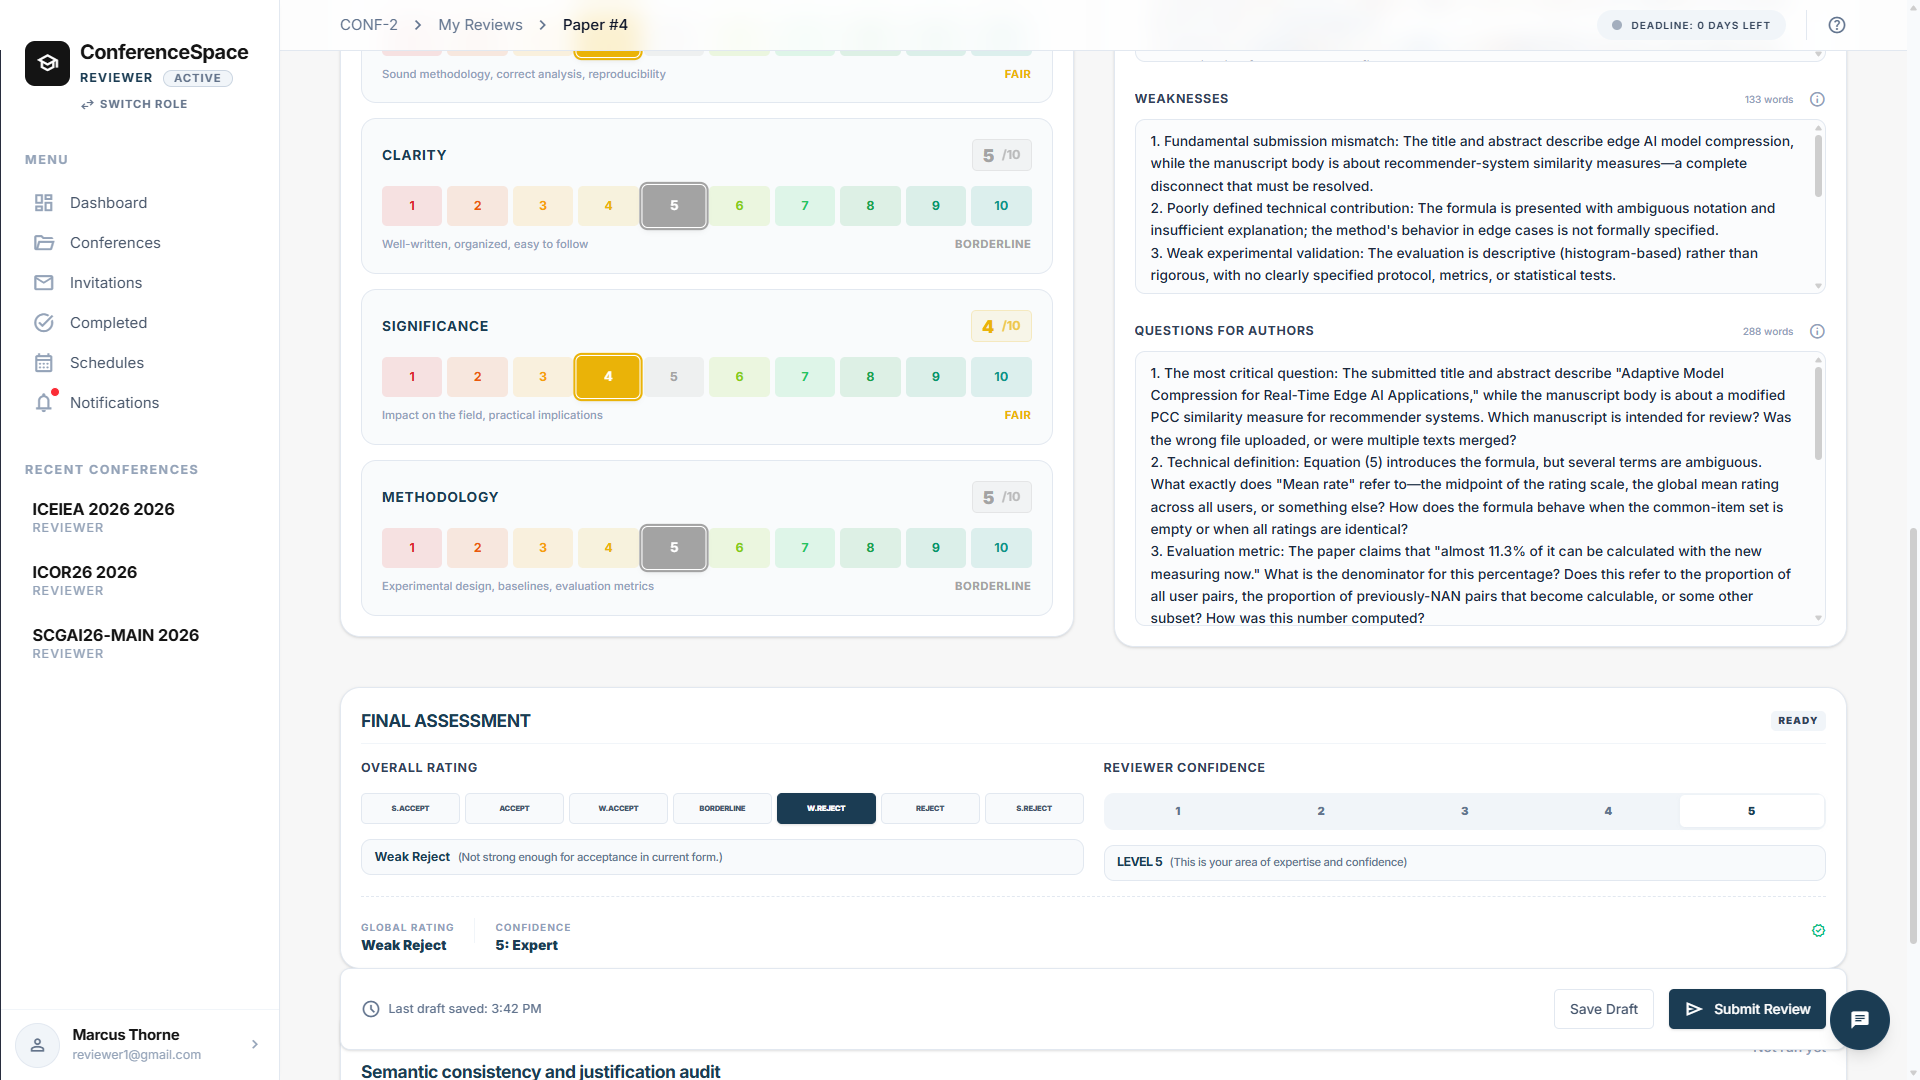
\includegraphics[width=0.95\textwidth]{images/chapter_3_uc05_reviewer_workspace_2.png}
  \caption{Không gian làm việc với biểu mẫu phản biện mở rộng của Phản biện viên}
  \label{fig:uc05-workspace-2-cut}
\end{figure}

Hình~\ref{fig:uc05-workspace-2-cut} trình bày một biến thể khác của không gian làm việc và biểu mẫu phản biện.

\begin{figure}[H]
  \centering
  \makebox[\textwidth][c]{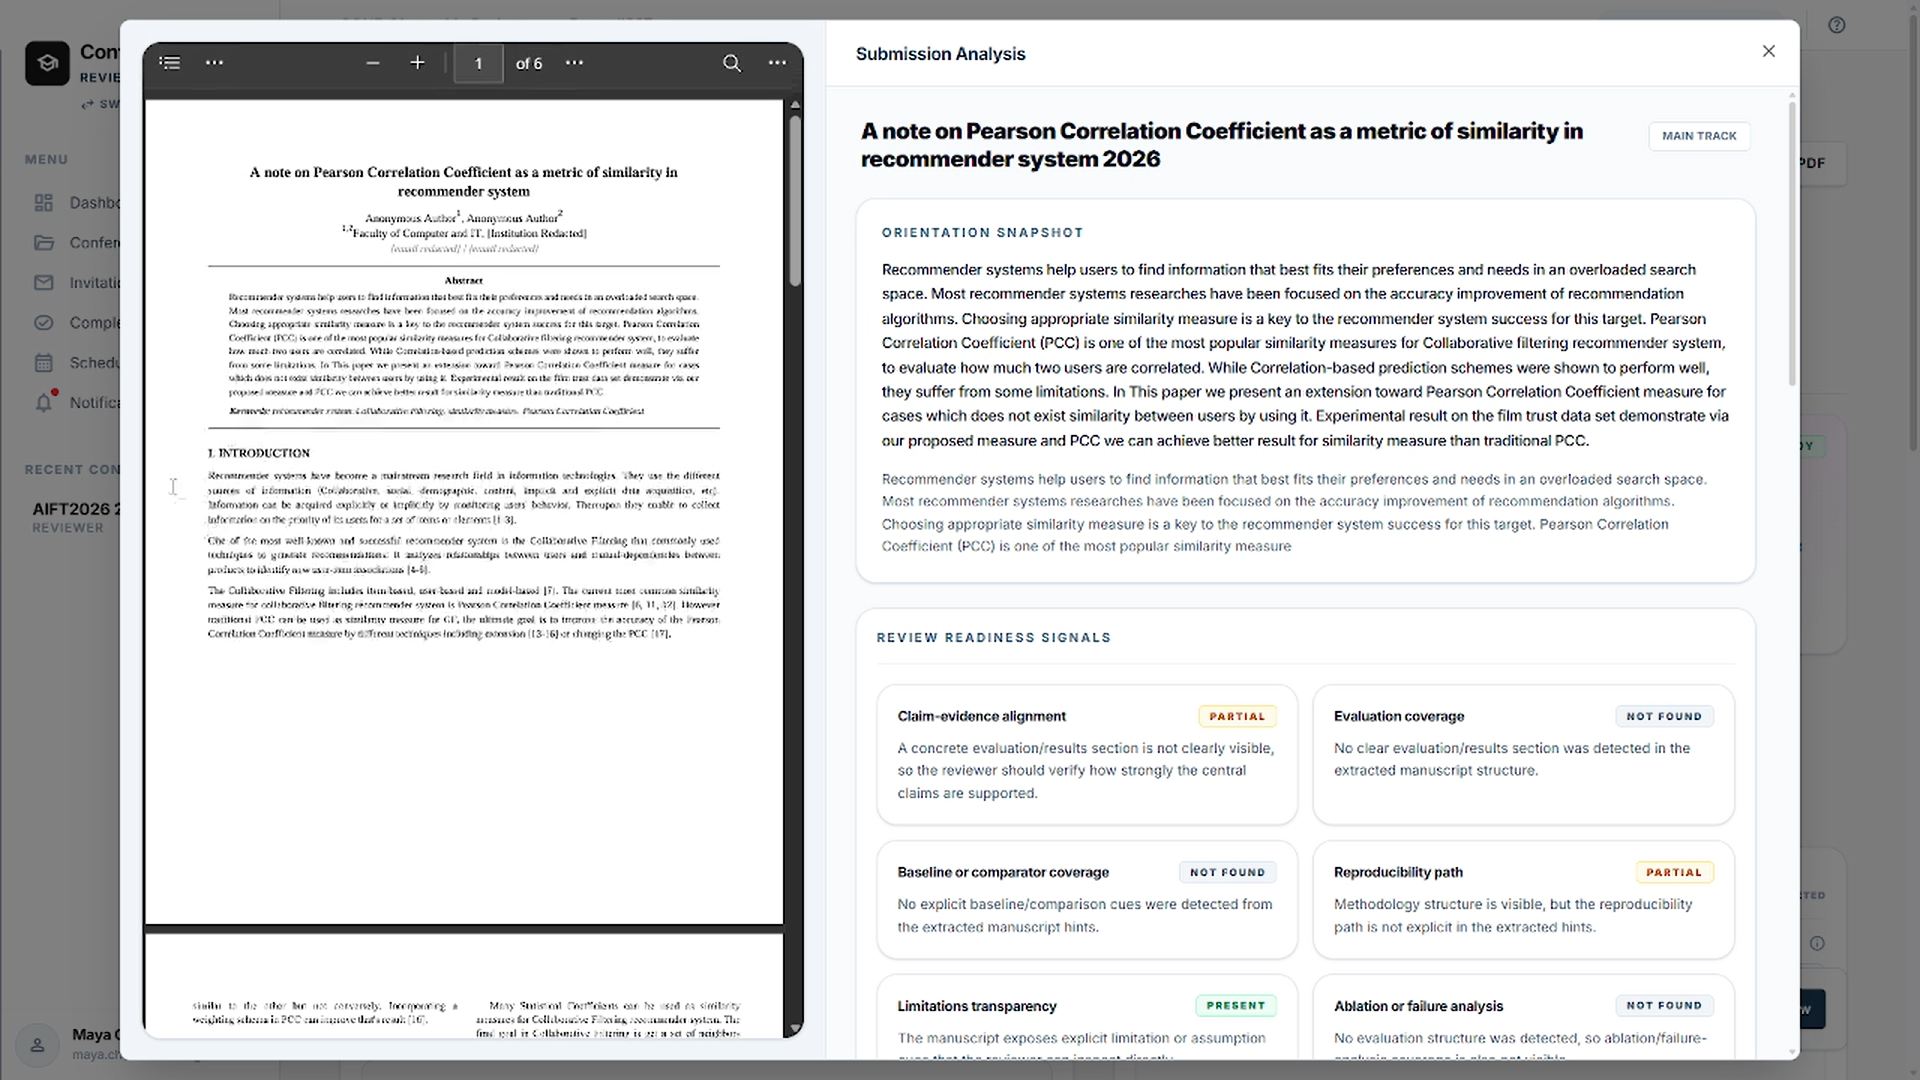
\includegraphics[width=1.10\textwidth]{images/chapter_3_uc05_reviewer_initial_analysis.png}}
  \caption{Bản định hướng đọc của Reviewer Initial Analysis}
  \label{fig:uc05-ria-cut}
\end{figure}

Hình~\ref{fig:uc05-ria-cut} thể hiện bản định hướng đọc do Reviewer Initial Analysis tạo ra để Phản biện viên tham khảo trước khi bắt đầu soạn phản biện.

\begin{figure}[H]
  \centering
  \makebox[\textwidth][c]{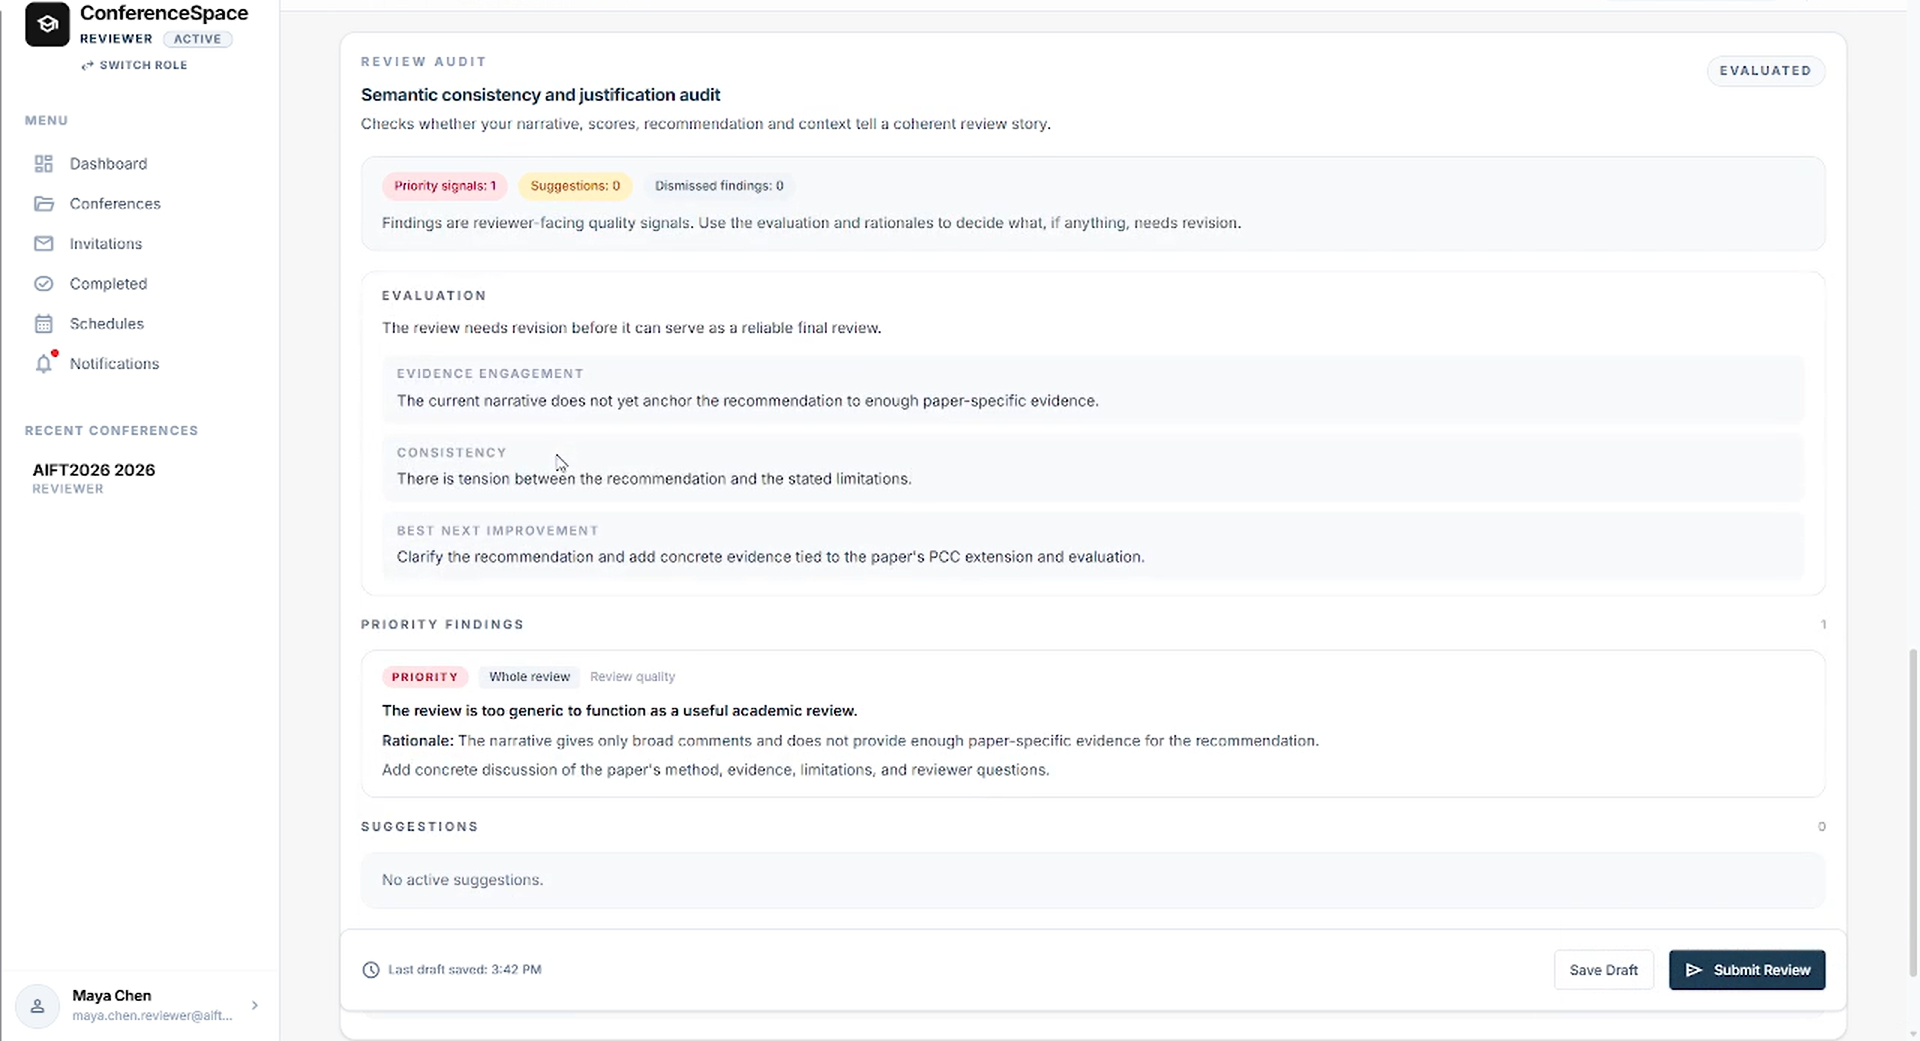
\includegraphics[width=1.10\textwidth]{images/chapter_3_uc05_reviewer_quality_auditor.png}}
  \caption{Bảng rà soát bản nháp của Review Quality Auditor}
  \label{fig:uc05-rqa-cut}
\end{figure}

Trước khi gửi phản biện, Phản biện viên xem bảng rà soát do Review Quality Auditor tạo ra tại Hình~\ref{fig:uc05-rqa-cut}.

Review Quality Auditor chạy trước khi gửi để đưa các phát hiện vào bảng rà soát. Phát hiện mức \textit{blocking} được làm nổi bật nhưng không ngăn Phản biện viên gửi phản biện. Nếu tác vụ rà soát không thể hoàn tất do lỗi dịch vụ, backend yêu cầu Phản biện viên xác nhận tiếp tục mà không có kết quả rà soát và ghi sự kiện này vào nhật ký. Hệ thống phân biệt phát hiện về chất lượng với lỗi không thể thực hiện bước rà soát: phát hiện chất lượng cung cấp thông tin để Phản biện viên xem xét, còn lỗi thực thi được thông báo rõ và ghi vào nhật ký.

\subsubsection{UC-06. Phân công phản biện có kiểm tra xung đột lợi ích}

Hệ thống chuẩn bị các cặp bài nộp--Phản biện viên, tính điểm phù hợp, loại các cặp có xung đột lợi ích khỏi đề xuất tự động và theo dõi số phân công được tạo trong cùng lượt chạy. Trước khi điều chỉnh hoặc xác nhận, Chủ tọa xem điểm số, lý do đối sánh, trạng thái kiểm tra xung đột lợi ích, tải phát sinh trong lượt chạy và danh sách bài chưa đủ Phản biện viên. Phản hồi \CodeBreak{AutoAssignResponse} không liệt kê đầy đủ từng cặp ứng viên bị loại. Khi Chủ tọa thêm đề xuất thủ công, backend kiểm tra quyền và trả cảnh báo xung đột lợi ích nhưng hiện chưa ngăn lưu; vì vậy, Chủ tọa phải xử lý cảnh báo trước khi xác nhận phương án.

\begin{figure}[H]
  \centering
  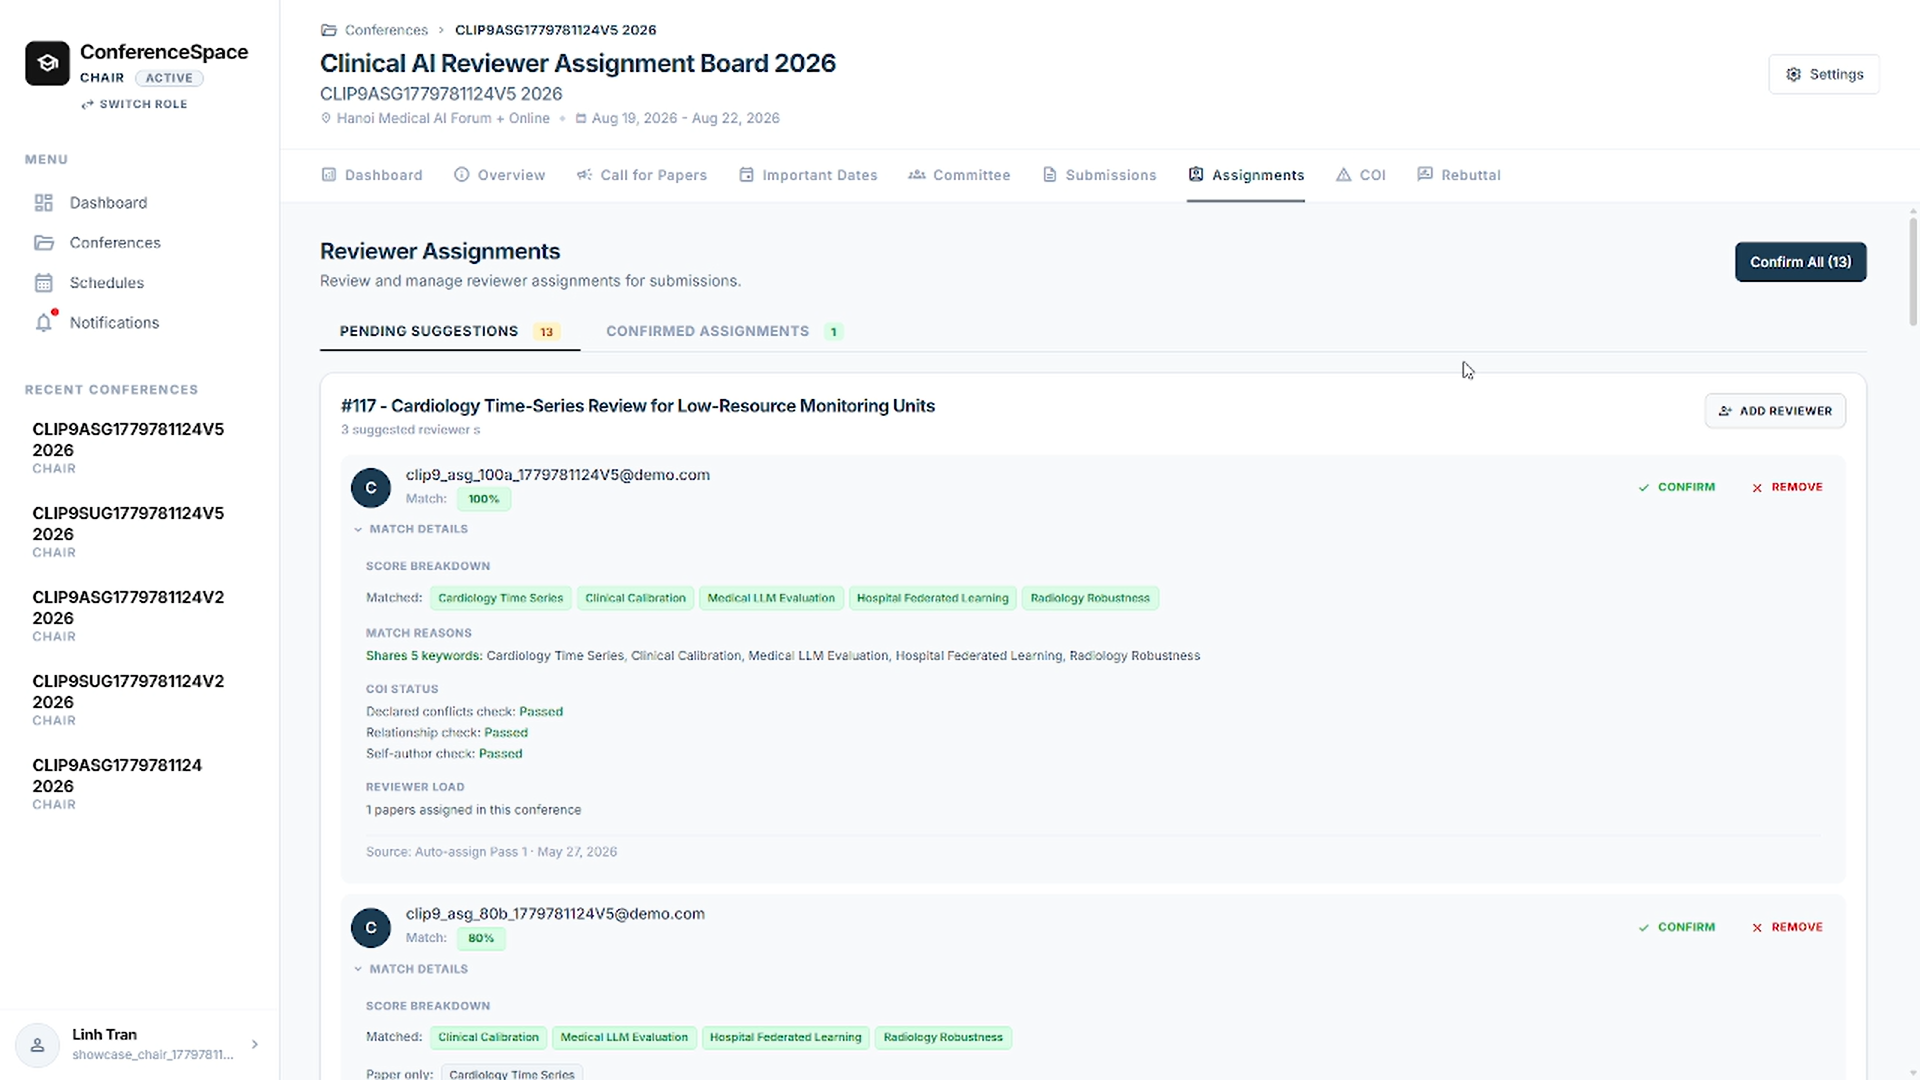
\includegraphics[width=0.95\textwidth]{images/chapter_3_uc06_assignment_dashboard.png}
  \caption{Giao diện bảng điều khiển quản lý phân công phản biện của Chủ tọa}
  \label{fig:uc06-dashboard-cut}
\end{figure}

Hình~\ref{fig:uc06-dashboard-cut} minh họa bảng điều khiển quản lý phân công phản biện của Chủ tọa.

\begin{figure}[H]
  \centering
  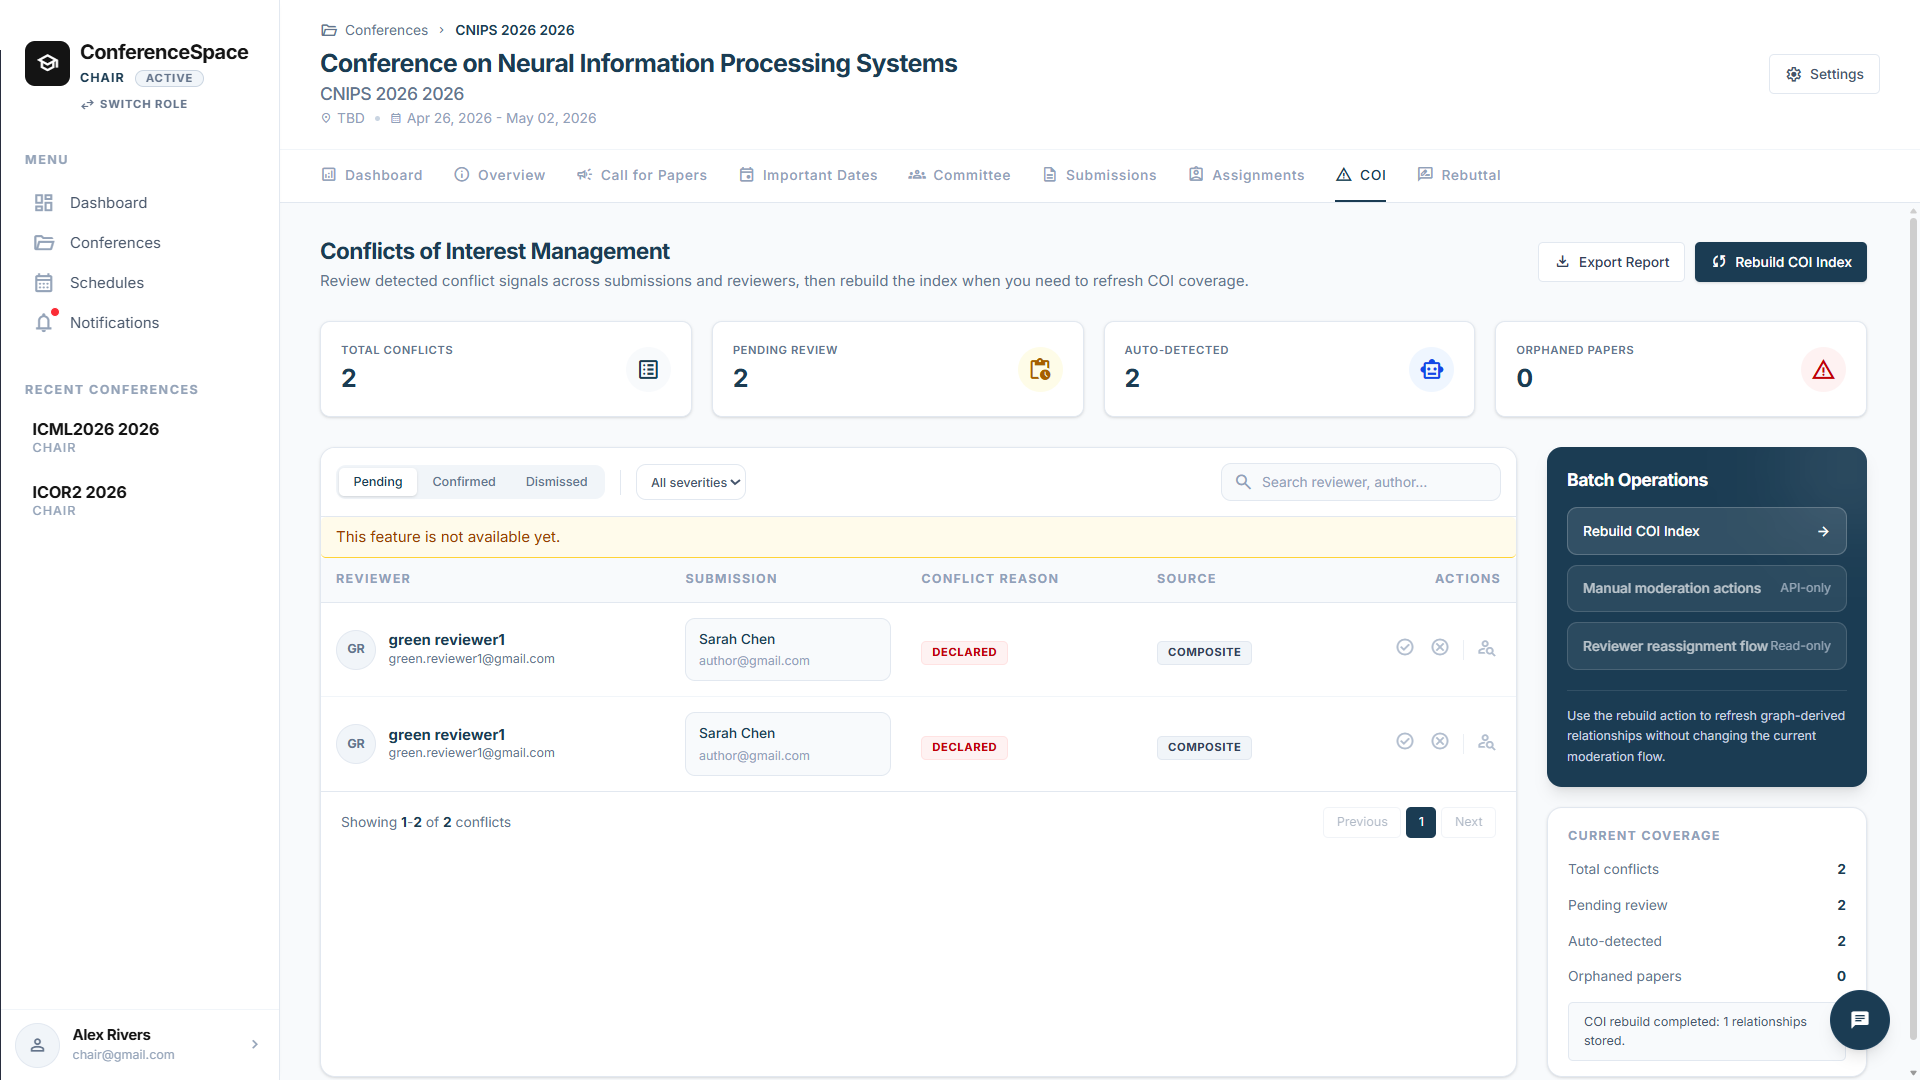
\includegraphics[width=0.95\textwidth]{images/chapter_3_uc06_coi_verification.png}
  \caption{Giao diện kiểm tra xung đột lợi ích giữa phản biện viên và bài nộp}
  \label{fig:uc06-coi-verification-cut}
\end{figure}

Hình~\ref{fig:uc06-coi-verification-cut} minh họa giao diện kiểm tra xung đột lợi ích giữa phản biện viên và bài nộp.

\begin{figure}[H]
  \centering
  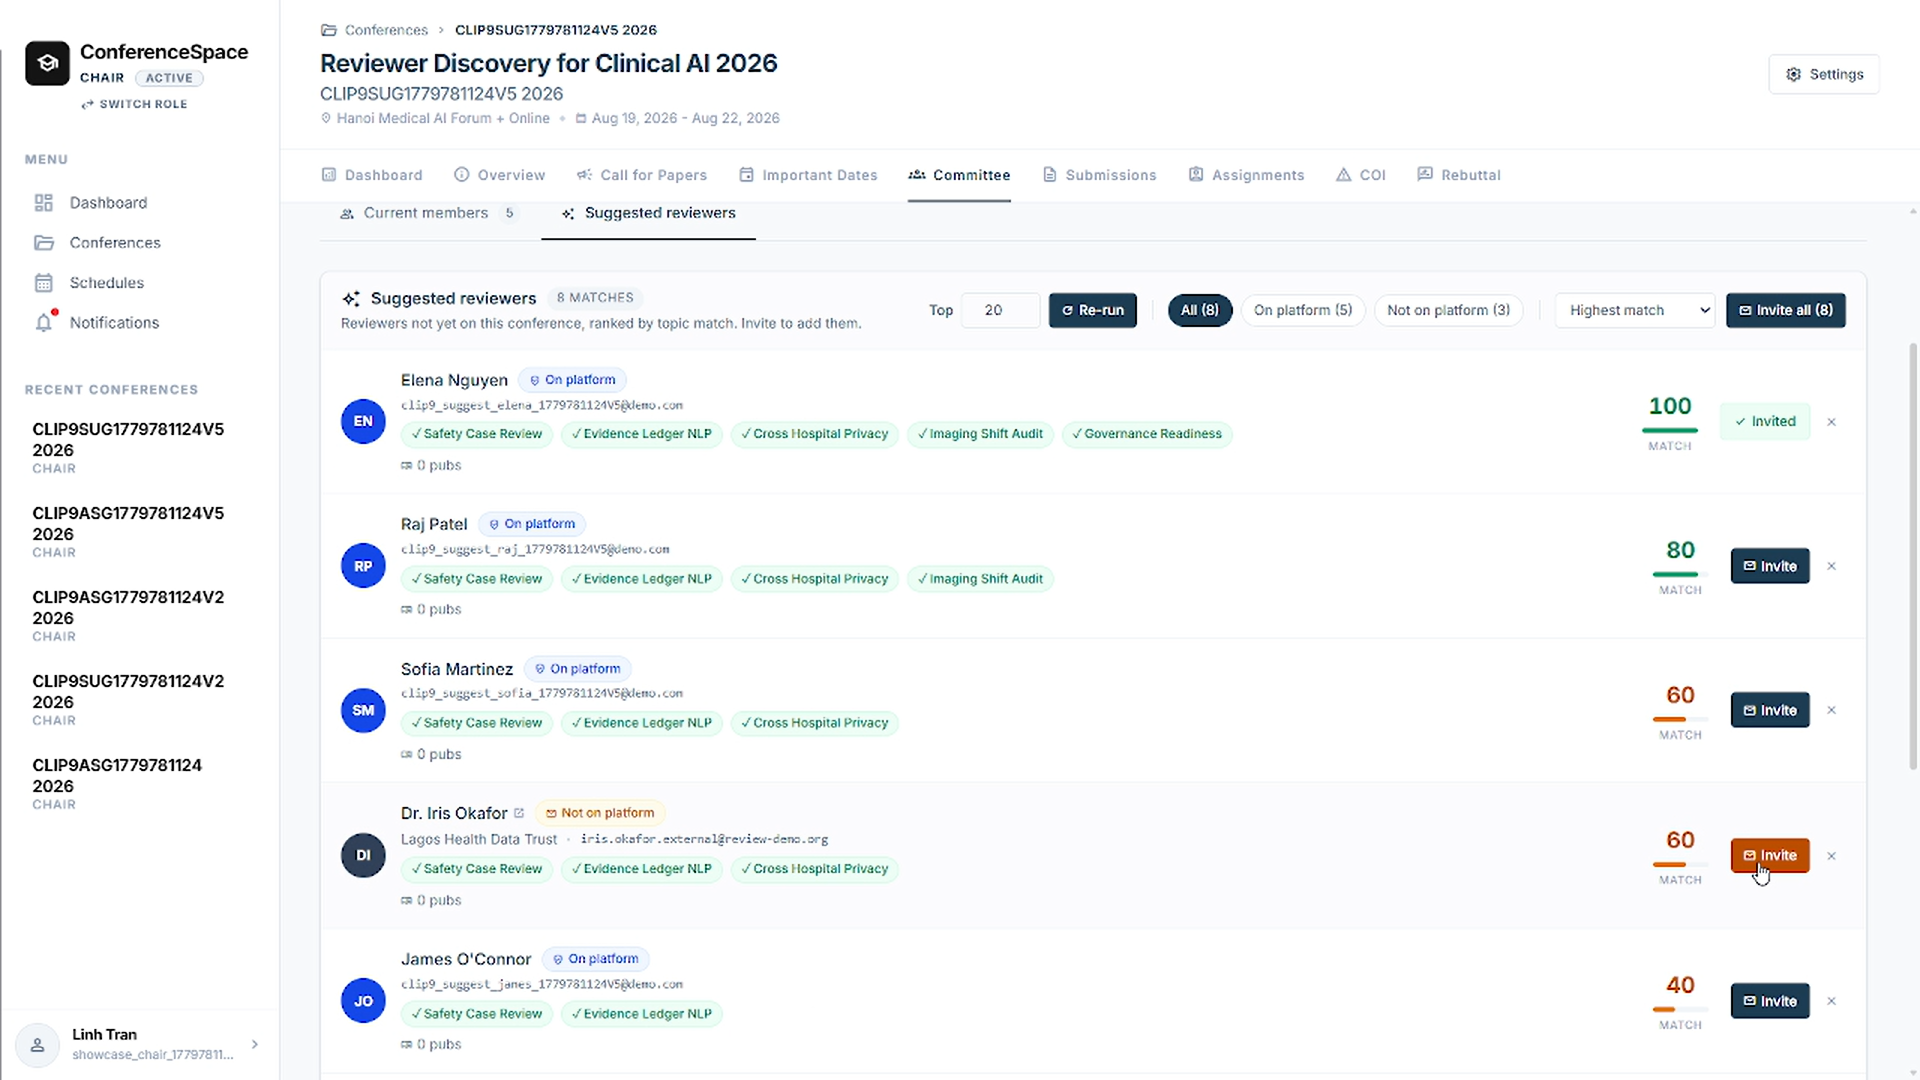
\includegraphics[width=0.95\textwidth]{images/chapter_3_uc06_assignment_suggestions.png}
  \caption{Danh sách đề xuất đối sánh và điểm phù hợp để Chủ tọa xem xét}
  \label{fig:uc06-suggestions-cut}
\end{figure}

Hình~\ref{fig:uc06-suggestions-cut} liệt kê các đề xuất đối sánh cùng điểm phù hợp để Chủ tọa xem xét trước khi xác nhận.

Công thức tính điểm, thủ tục phân công, lượt dự phòng và các trường hợp ngoại lệ được trình bày tại Mục~\ref{subsec:ch3-matching-cut}. Thuật toán tự động không nới ràng buộc xung đột lợi ích, kể cả khi hệ thống không tìm được đủ Phản biện viên; luồng thêm đề xuất thủ công hiện dùng cảnh báo thay cho cưỡng chế tại thời điểm ghi dữ liệu.

\subsubsection{UC-07. Quản lý hội nghị và theo dõi tiến độ}

Chủ tọa cấu hình thông tin hội nghị, chuyên đề, hạn chót nộp bài, biểu mẫu phản biện và chính sách; mời thành viên hội đồng chương trình; theo dõi số bài, tiến độ phản biện và các trường hợp cần xử lý. Hệ thống từ chối cấu hình thiếu trường bắt buộc, hạn chót nộp bài không hợp lệ hoặc thao tác của người dùng không có quyền. Bảng điều khiển hỗ trợ nhận biết các trường hợp cần xử lý nhưng không tự chuyển giai đoạn hoặc ra quyết định thay Chủ tọa.

\begin{figure}[H]
  \centering
  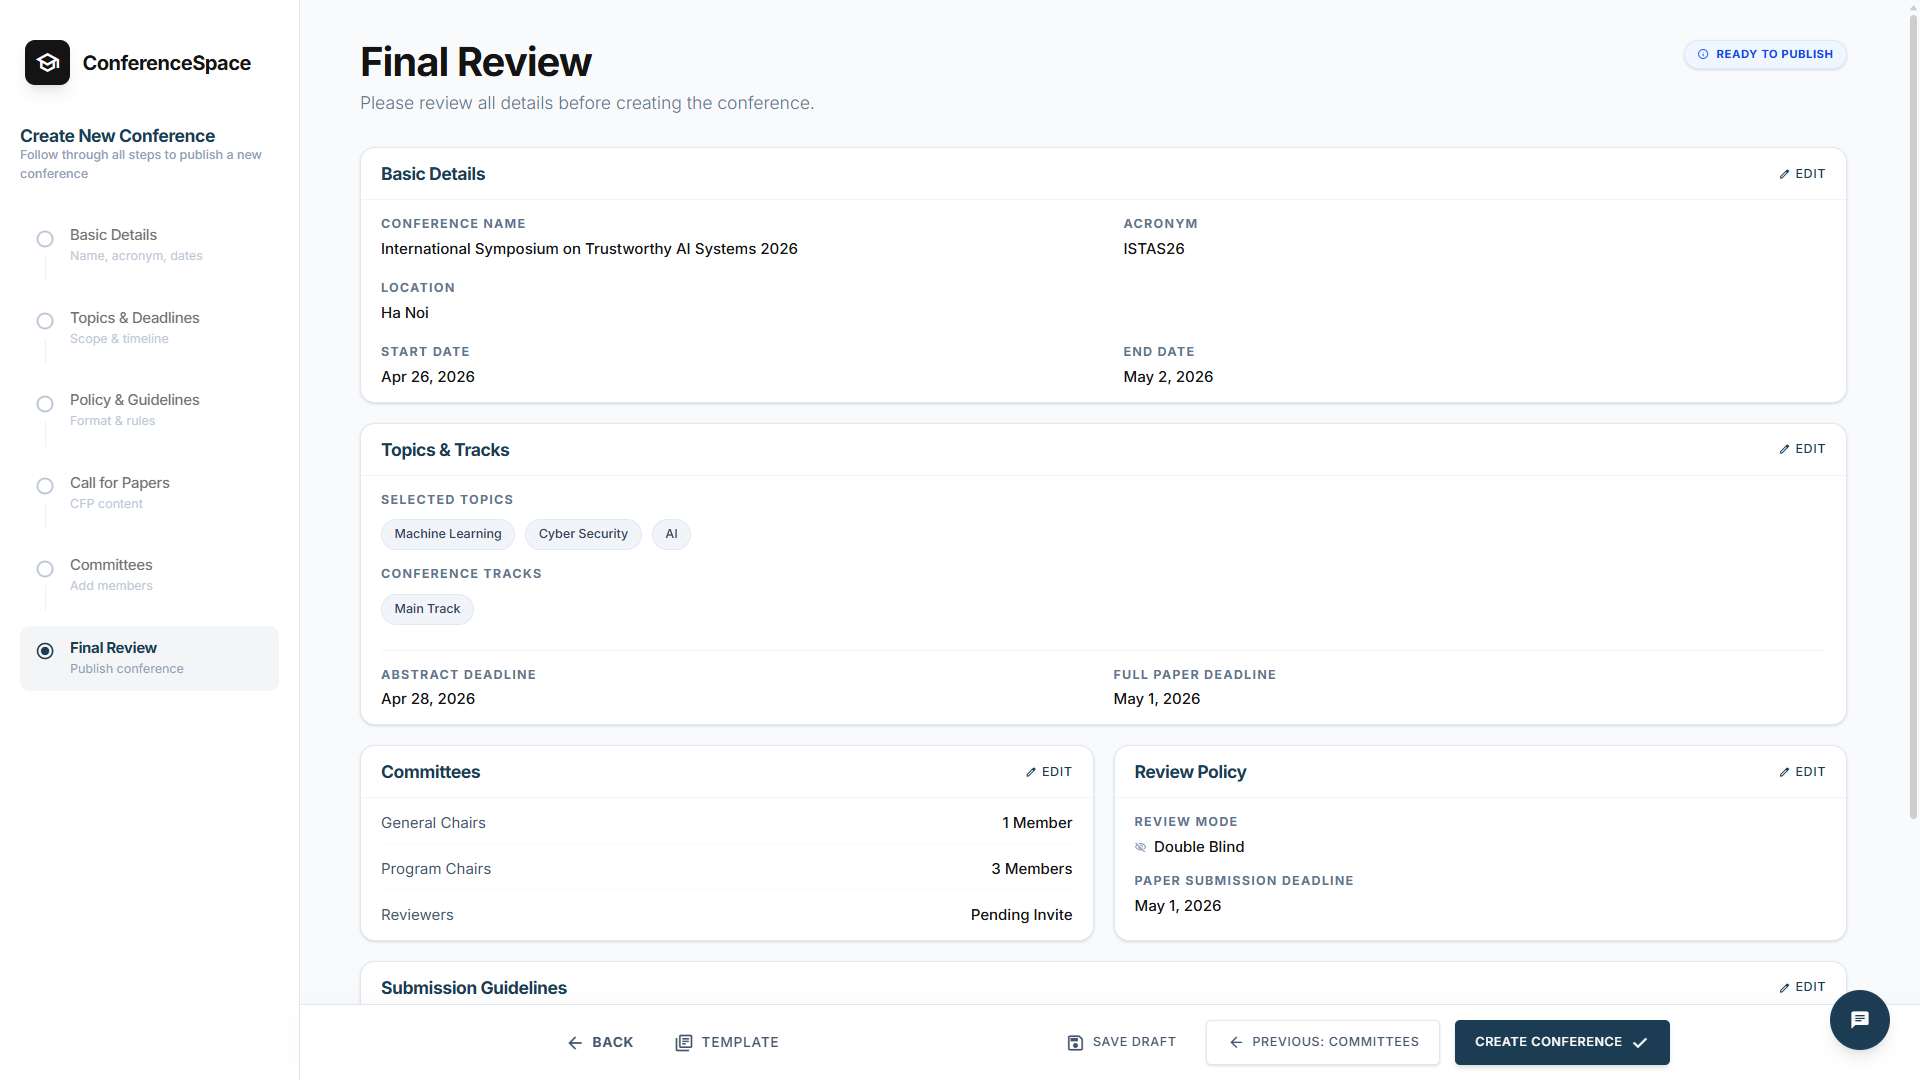
\includegraphics[width=0.95\textwidth]{images/chapter_3_uc07_conference_config.png}
  \caption{Giao diện thiết lập cấu hình thông tin và hạn chót nộp bài hội nghị của Chủ tọa}
  \label{fig:uc07-config-cut}
\end{figure}

Hình~\ref{fig:uc07-config-cut} thể hiện giao diện thiết lập cấu hình thông tin và hạn chót nộp bài hội nghị.

\begin{figure}[H]
  \centering
  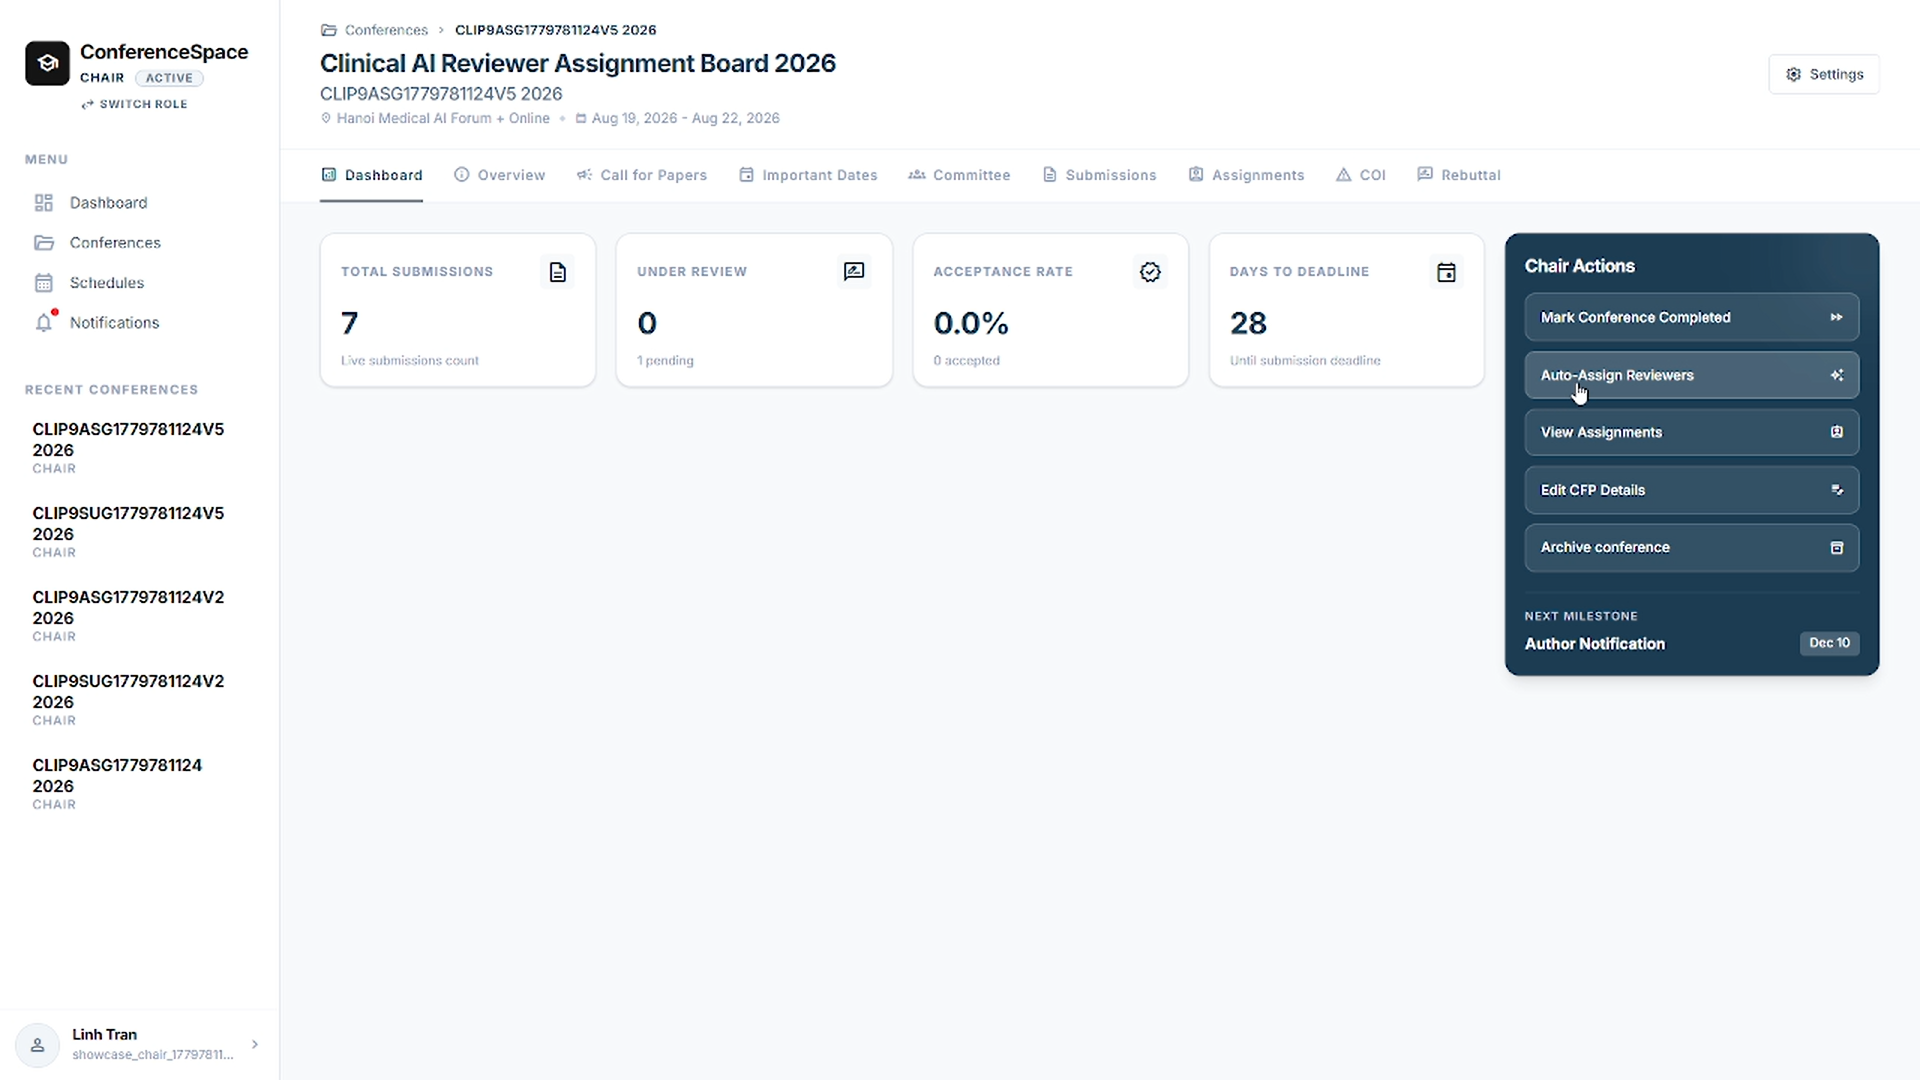
\includegraphics[width=0.95\textwidth]{images/chapter_3_uc07_chair_dashboard.png}
  \caption{Bảng điều khiển tiến độ hội nghị của Chủ tọa}
  \label{fig:uc07-dashboard-cut}
\end{figure}

Hình~\ref{fig:uc07-dashboard-cut} cung cấp cái nhìn tổng quan về hoạt động điều phối, bổ sung cho các hình chuyên biệt về đối sánh và hỗ trợ quyết định.

\begin{figure}[H]
  \centering
  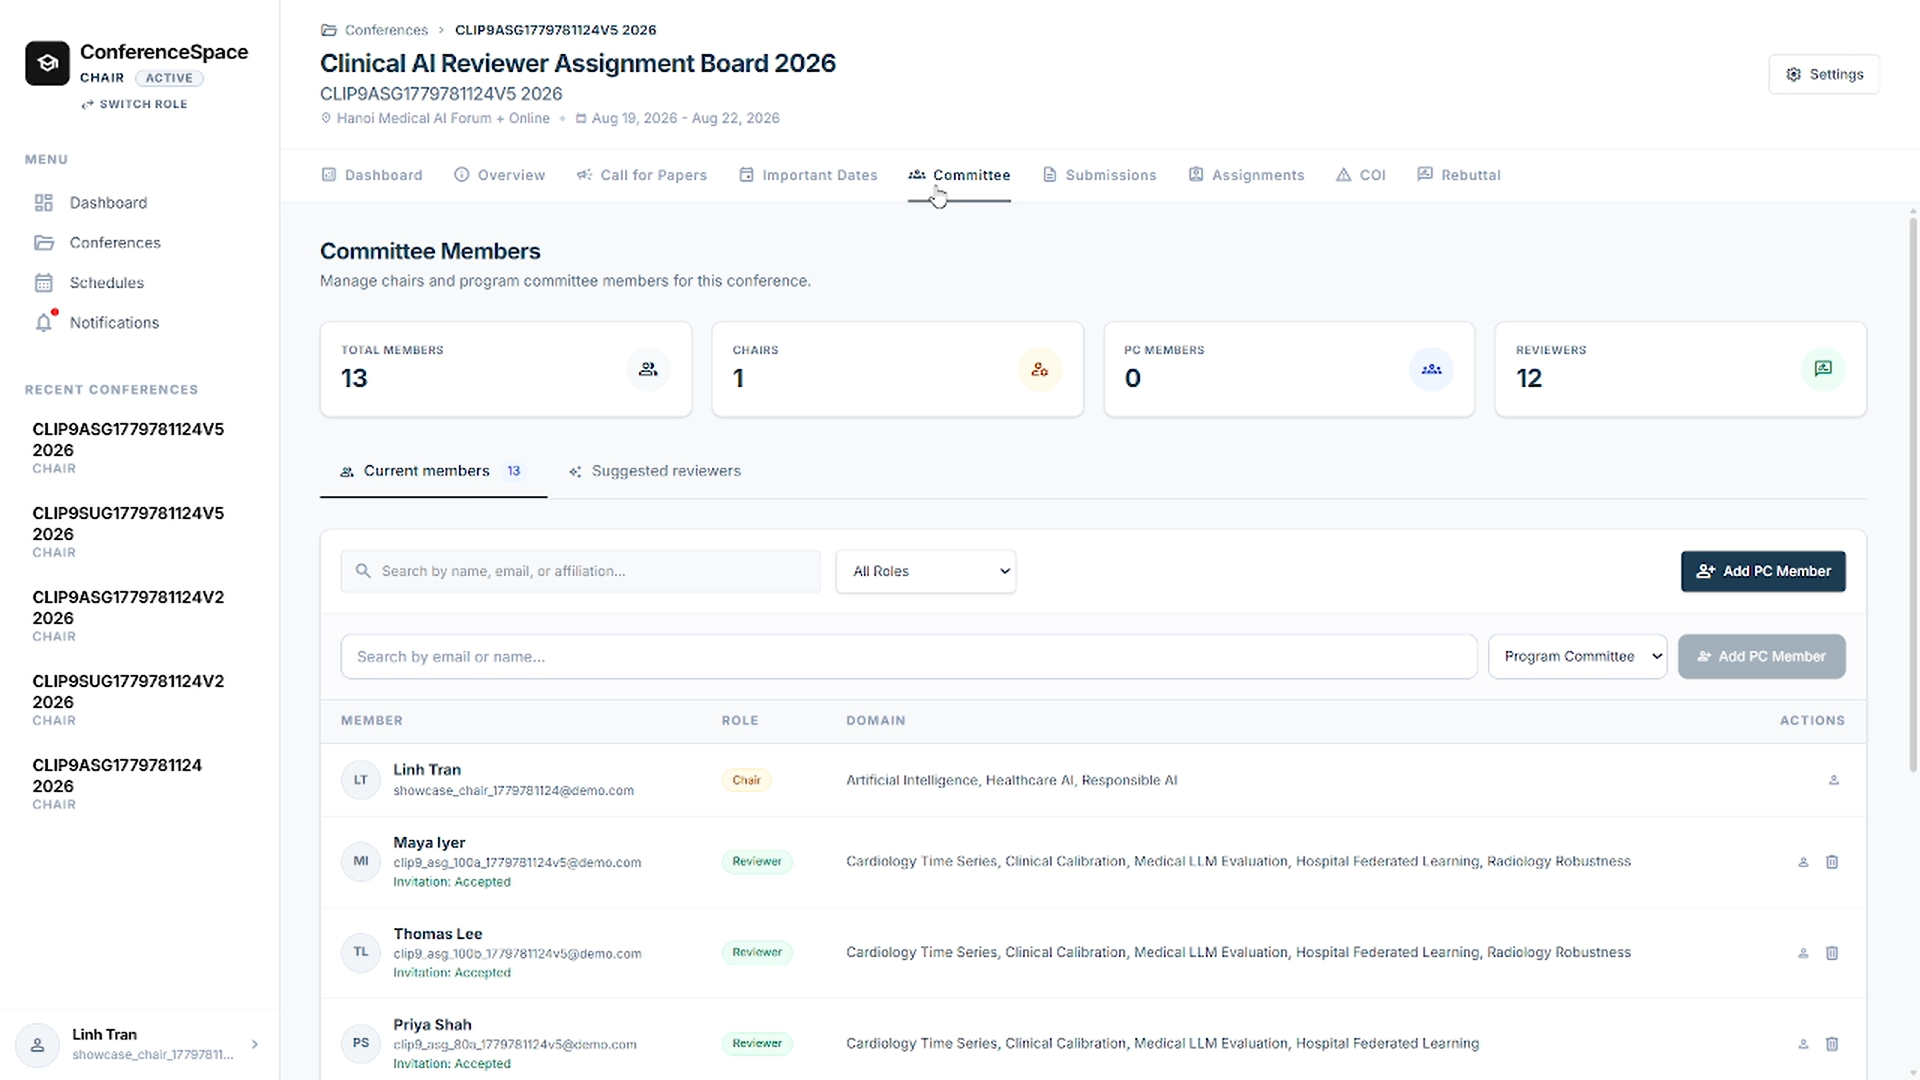
\includegraphics[width=0.95\textwidth]{images/chapter_3_uc07_committee_management.png}
  \caption{Giao diện quản lý ban chương trình và trạng thái lời mời phản biện viên}
  \label{fig:uc07-committee-cut}
\end{figure}

Hình~\ref{fig:uc07-committee-cut} minh họa giao diện quản lý ban chương trình và trạng thái lời mời phản biện viên.

\subsubsection{UC-08. Trao đổi theo bài nộp}

Chủ tọa hoặc Đồng chủ tọa mở giai đoạn phản hồi và kết thúc giai đoạn này trước khi ra quyết định; giai đoạn thảo luận chỉ được mở khi cấu hình hội nghị cho phép. Phản biện viên được phân công có thể tạo chuỗi thảo luận. Tác giả của bài và Phản biện viên trao đổi trong chuỗi tương ứng, còn Chủ tọa xem toàn bộ lịch sử ở chế độ giám sát. Sau khi đọc phản hồi, Phản biện viên có thể cập nhật điểm, khuyến nghị và nhận xét của bài mình phụ trách. Backend kiểm tra quan hệ giữa người dùng, bài nộp và chuỗi thảo luận trước mỗi thao tác. Nội dung trao đổi cùng đánh giá cập nhật được lưu với bài nộp và trở thành nguồn bằng chứng cho Chair Decision Copilot.

\begin{figure}[H]
  \centering
  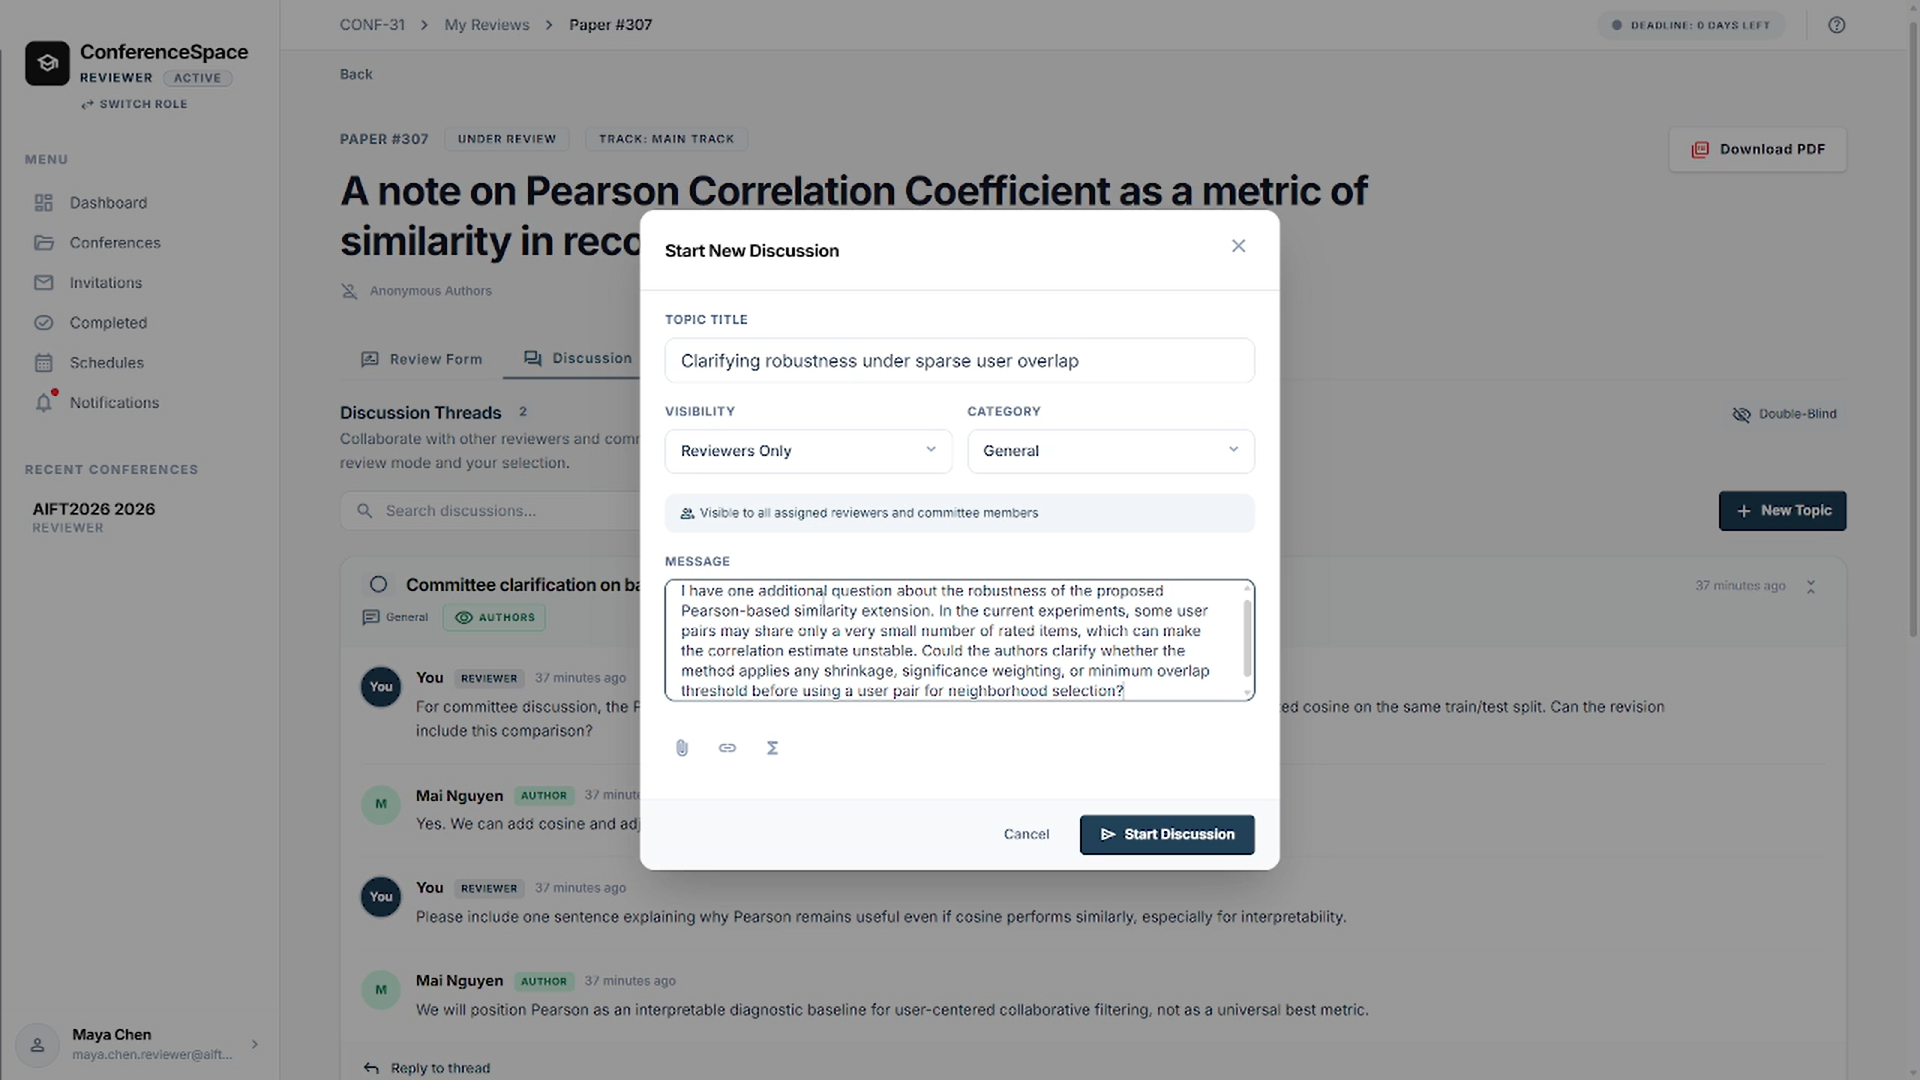
\includegraphics[width=0.95\textwidth]{images/chapter_3_uc08_create_discussion.png}
  \caption{Giao diện khởi tạo chủ đề thảo luận mới cho bài nộp}
  \label{fig:uc08-create-discussion-cut}
\end{figure}

Hình~\ref{fig:uc08-create-discussion-cut} minh họa giao diện khởi tạo chủ đề thảo luận mới cho bài nộp.

\begin{figure}[H]
  \centering
  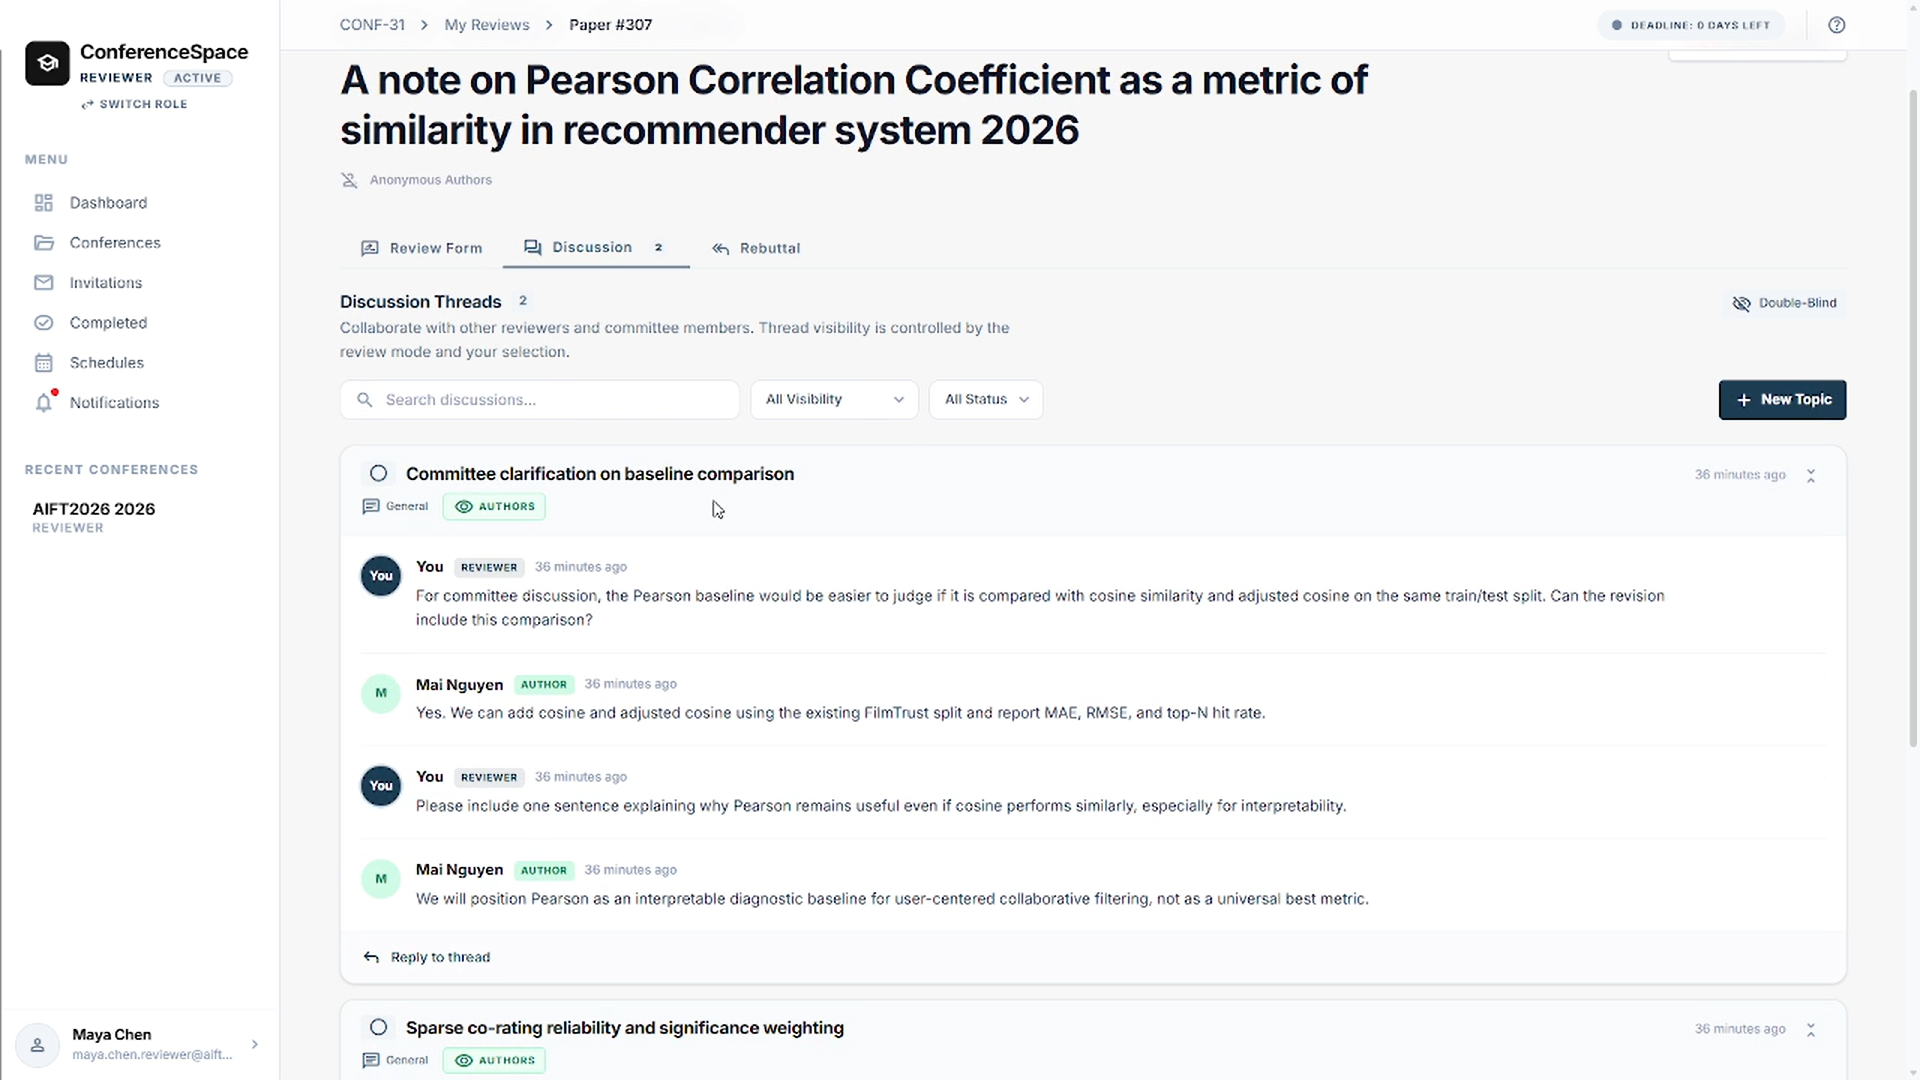
\includegraphics[width=0.95\textwidth]{images/chapter_3_uc08_discussion_chat.png}
  \caption{Giao diện hiển thị danh sách và trao đổi nội dung thảo luận}
  \label{fig:uc08-discussion-chat-cut}
\end{figure}

Hình~\ref{fig:uc08-discussion-chat-cut} thể hiện giao diện hiển thị danh sách chủ đề và nội dung trao đổi trong từng chủ đề.

\subsubsection{UC-09. Tổng hợp bằng chứng hỗ trợ Chủ tọa ra quyết định}

Backend tập hợp điểm số, bản phản biện, phản hồi của Tác giả, thay đổi sau phản hồi và nội dung thảo luận. Chair Decision Copilot tổ chức các nguồn này thành bản tổng hợp gồm điểm đồng thuận, bất đồng, vấn đề còn mở và bằng chứng liên quan. Chủ tọa đối chiếu bản tổng hợp với dữ liệu gốc rồi tự ghi nhận quyết định cuối cùng. Khi bộ bằng chứng thay đổi, hệ thống đánh dấu kết quả cũ là không còn hiệu lực.

\begin{figure}[H]
  \centering
  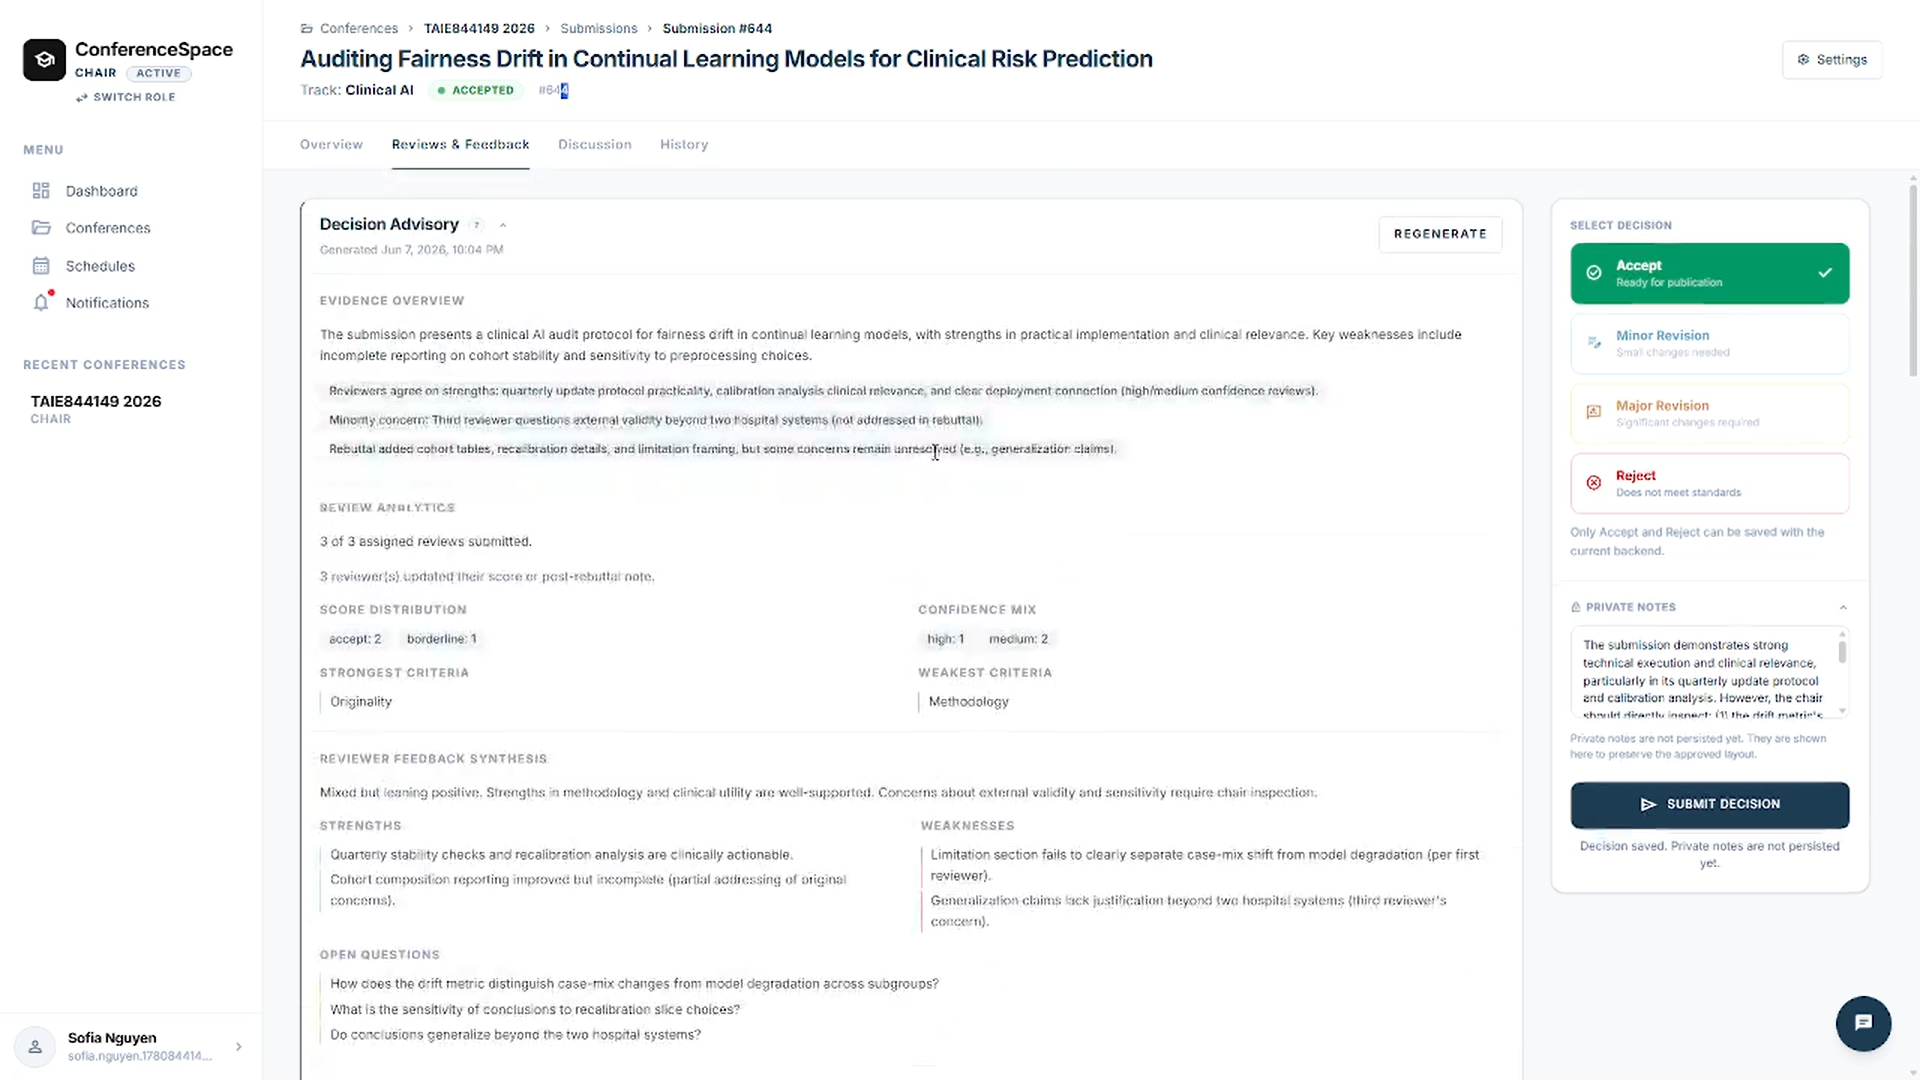
\includegraphics[width=0.95\textwidth]{images/chapter_3_uc09_decision_support.png}
  \caption{Giao diện tổng hợp bằng chứng và ghi nhận quyết định của Chủ tọa}
  \label{fig:uc09-decision-cut}
\end{figure}

Hình~\ref{fig:uc09-decision-cut} minh họa giao diện tổng hợp bằng chứng và ghi nhận quyết định của Chủ tọa.

Chair Decision Copilot không tạo khuyến nghị chấp nhận hoặc từ chối. Khi dịch vụ AI gặp lỗi, Chủ tọa vẫn có thể đọc trực tiếp các nguồn bằng chứng và tiếp tục quy trình nghiệp vụ.

\subsubsection{UC-10. Truy vấn trạng thái và hướng dẫn theo ngữ cảnh bằng Chatbot Agent}

Chatbot Agent nhận câu hỏi, lịch sử hội thoại và ngữ cảnh trang hiện tại. Nếu câu hỏi cần dữ liệu nghiệp vụ, Chatbot Agent gọi công cụ truy vấn để gửi yêu cầu có cấu trúc đến backend; backend kiểm tra mã xác thực, tài nguyên, trường dữ liệu, bộ lọc và quyền của người dùng trước khi trả phần dữ liệu tối thiểu được phép. Chatbot Agent dùng kết quả này để tạo câu trả lời phù hợp với vai trò và không truy cập trực tiếp cơ sở dữ liệu.

Backend từ chối yêu cầu vượt quá quyền truy cập; Chatbot Agent thông báo rõ khi câu hỏi nằm ngoài phạm vi chức năng được hỗ trợ. Khi công cụ gặp lỗi, hệ thống trả trạng thái lỗi thay vì tạo dữ liệu không có căn cứ. Các kịch bản hội thoại ở Chương 4 kiểm tra ranh giới này trong phạm vi tài nguyên và vai trò đã chọn.

\begin{figure}[H]
  \centering
  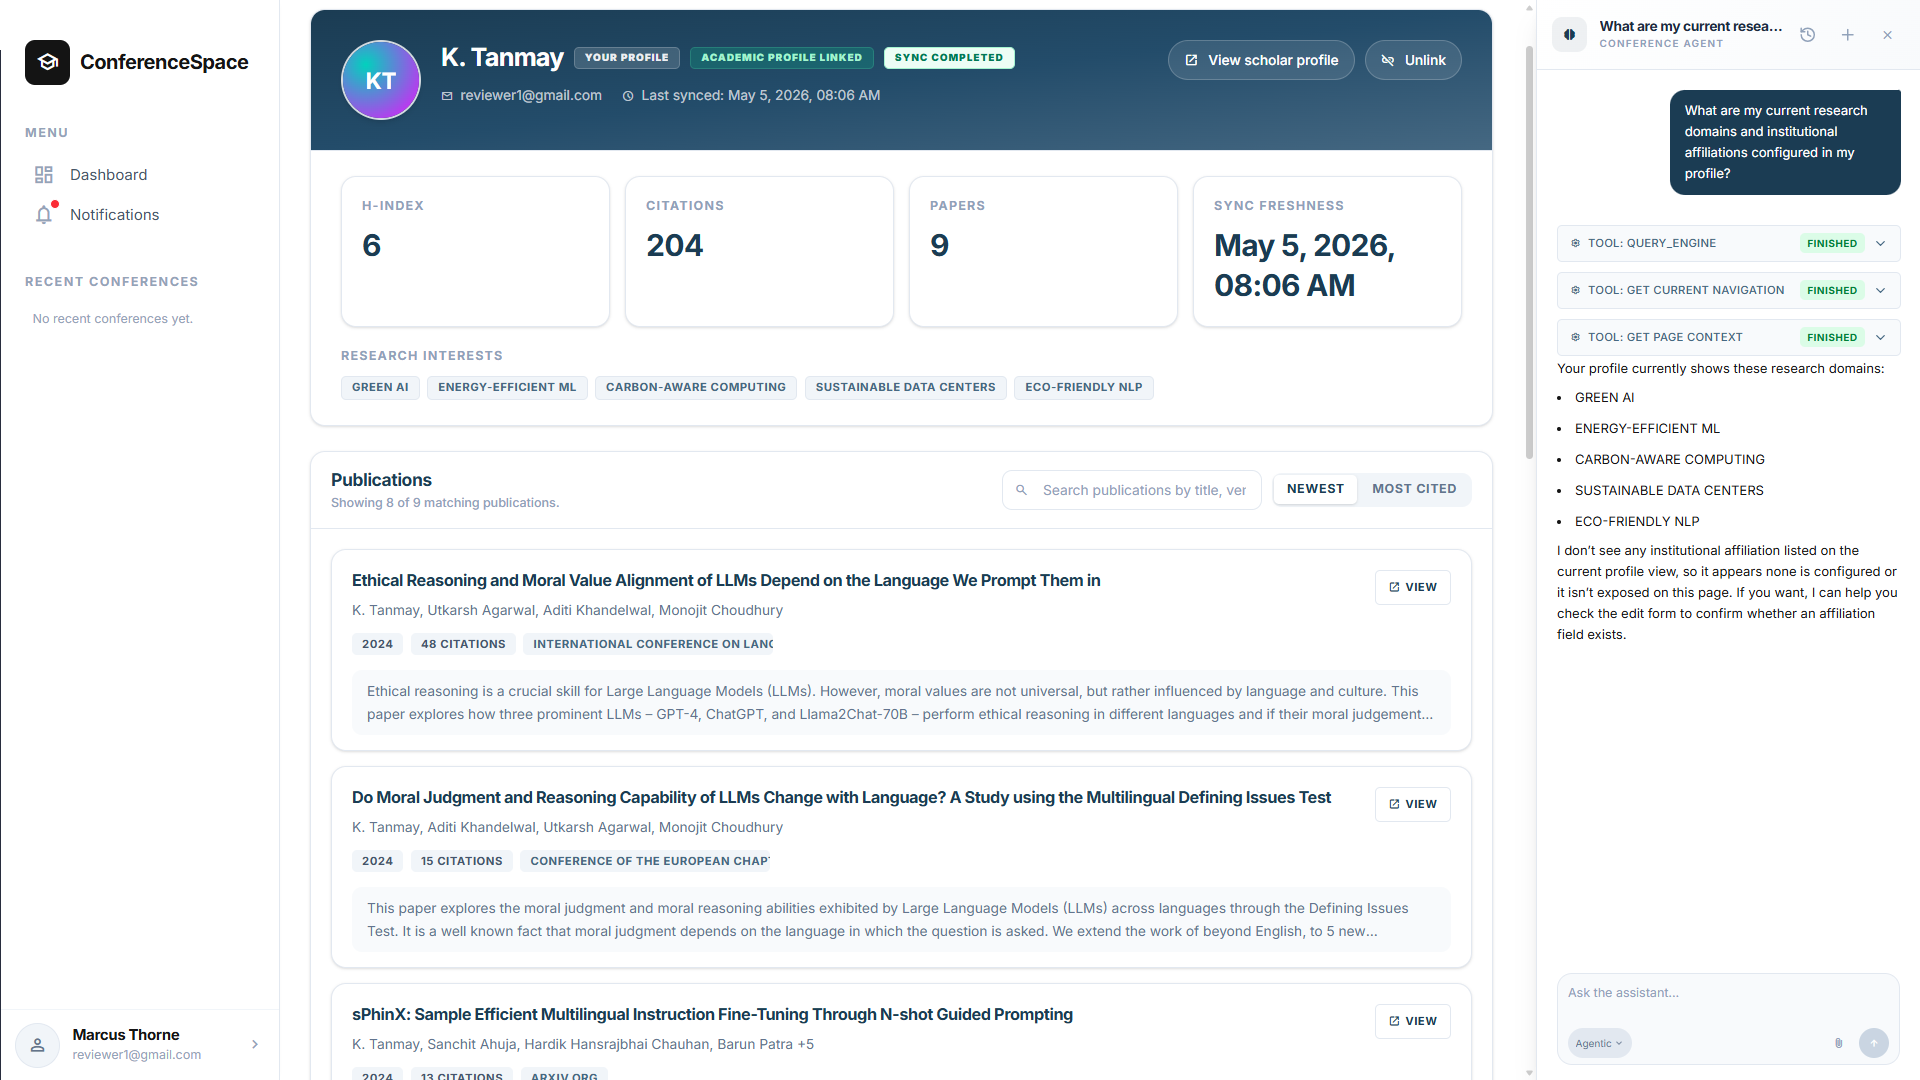
\includegraphics[width=0.95\textwidth]{images/chapter_3_uc10_chatbot_interface.png}
  \caption{Giao diện hội thoại và hỗ trợ tra cứu thông tin của Chatbot Agent}
  \label{fig:uc10-chatbot-cut}
\end{figure}

Hình~\ref{fig:uc10-chatbot-cut} minh họa giao diện hội thoại của Chatbot Agent trong luồng này.

\section{Thiết kế kỹ thuật}

\subsection{Kiến trúc tổng thể}
\label{subsec:ch3-architecture-cut}

ConferenceSpace gồm giao diện web Next.js, backend Go/Gin, dịch vụ AI FastAPI, PostgreSQL, Redis, Neo4j và cổng Caddy. Backend nghiệp vụ là một ứng dụng nguyên khối có kiến trúc phân lớp; nhóm không chia nhỏ nghiệp vụ thành các vi dịch vụ khi chưa có nhu cầu vận hành tương ứng. Dịch vụ AI và các kho dữ liệu được tách tại ranh giới triển khai vì có vòng đời, tải xử lý và yêu cầu truy cập khác với backend.

\begin{figure}[H]
  \centering
  \begin{adjustbox}{max width=\textwidth}
    \begin{tikzpicture}[node distance=12mm and 18mm, >=Latex]
      \node[prismNode] (browser) at (0,0) {Trình duyệt};
      \node[prismNode] (caddy) at (0,-2.2) {Caddy};
      \node[prismNode] (web) at (0,-4.4) {Next.js};
      \node[prismNode] (backend) at (0,-6.6) {Backend Go/Gin};
      \node[prismNode] (postgres) at (-6.4,-9.2) {PostgreSQL};
      \node[prismNode] (neo4j) at (-2.1,-9.2) {Neo4j};
      \node[prismNode] (ai) at (2.1,-9.2) {Dịch vụ AI};
      \node[prismNode] (external) at (6.4,-9.2) {Nguồn dữ liệu học thuật bên ngoài};
      \node[prismNode] (redis) at (0,-11.8) {Redis};
      \node[prismNode] (model) at (4.3,-11.8) {Nhà cung cấp mô hình};
      \draw[prismArrow] (browser) -- (caddy);
      \draw[prismArrow] (caddy) -- (web);
      \draw[prismArrow] (web) -- (backend);
      \draw[prismArrow] (web) -- node[prismEdgeLabel] {API hội thoại} (ai);
      \draw[prismArrow] (backend) -- (postgres);
      \draw[prismArrow] (backend) -- (neo4j);
      \draw[prismArrow] (backend) -- (ai);
      \draw[prismDashedArrow, bend left=24] (ai) to node[prismEdgeLabel] {endpoint truy vấn của backend} (backend);
      \draw[prismArrow] (backend) -- (external);
      \draw[prismArrow] (ai) -- (redis);
      \draw[prismArrow] (ai) -- (model);
      \draw[prismDashedArrow] (ai) -- node[prismEdgeLabel] {kết quả cần truy vết} (postgres);
    \end{tikzpicture}
  \end{adjustbox}
  \caption{Kiến trúc dịch vụ và ranh giới dữ liệu của ConferenceSpace}
  \label{fig:ch3-architecture-cut}
\end{figure}

Backend là ranh giới nghiệp vụ chính đối với dữ liệu và cập nhật trạng thái. Giao diện không truy cập trực tiếp cơ sở dữ liệu hoặc nhà cung cấp mô hình; tuy nhiên, Next.js có luồng giao tiếp trực tiếp với dịch vụ AI cho hội thoại. Khi Chatbot Agent cần dữ liệu nghiệp vụ, dịch vụ AI gọi endpoint truy vấn của backend bằng mã xác thực của người dùng và mã xác thực liên dịch vụ; backend tiếp tục kiểm tra danh mục tài nguyên và phân quyền theo vai trò trong hội nghị (RBAC). Sơ đồ vì vậy tách luồng hội thoại Next.js--AI khỏi luồng truy vấn dữ liệu AI--backend.

\subsection{Thiết kế giao diện web và trải nghiệm theo vai trò}
\label{subsec:ch3-web-cut}

Giao diện được tổ chức theo không gian làm việc của từng vai trò. Không gian Tác giả kết nối hoạt động khám phá hội nghị, nộp và quản lý bài; không gian Phản biện viên kết nối lời mời, bài được phân công, trình soạn phản biện và thảo luận; không gian Chủ tọa kết nối cấu hình, phân công, giám sát tiến độ và ra quyết định. Chatbot Agent và thông báo xuất hiện trong cả ba không gian nhưng dùng cùng ngữ cảnh xác thực và quyền trên tài nguyên.

Giao diện sử dụng Next.js App Router, React, TypeScript, Radix UI và Tailwind CSS \cite{ch3ref1,ch3ref3,ch3ref4,ch3ref5}. Các luồng dài được chia thành từng bước; trạng thái quan trọng được thể hiện bằng nhãn và bảng; thao tác gửi bài, gửi phản biện và lưu quyết định yêu cầu người dùng xác nhận. Đầu ra AI được trình bày dưới dạng bản nháp, cảnh báo hoặc bản tổng hợp cần kiểm tra, thay vì kết luận chính thức.

\subsection{Thiết kế backend, API và phân quyền}
\label{subsec:ch3-backend-cut}

Backend áp dụng kiến trúc phân lớp. Tầng điều khiển tiếp nhận yêu cầu HTTP; tầng dịch vụ thực thi nghiệp vụ; tầng lưu trữ làm việc với PostgreSQL; tầng tích hợp (client) kết nối dịch vụ AI, Neo4j, nguồn dữ liệu học thuật và thư điện tử. Nghiệp vụ phân công được tách thành miền riêng để logic tính điểm, đối sánh và phát hiện xung đột lợi ích có thể được kiểm thử độc lập.

\begin{figure}[H]
  \centering
  \begin{adjustbox}{max width=0.9\textwidth}
    \begin{tikzpicture}[node distance=12mm and 18mm, >=Latex]
      \node[prismNode] (router) at (0,0) {Bộ định tuyến Gin};
      \node[prismNode] (middleware) at (0,-2.2) {Middleware xác thực và ghi nhật ký};
      \node[prismNode] (controller) at (0,-4.4) {Tầng điều khiển};
      \node[prismNode] (service) at (0,-6.6) {Tầng dịch vụ};
      \node[prismNode] (storage) at (-4.2,-9.0) {Tầng lưu trữ};
      \node[prismNode] (assignment) at (0,-9.0) {Miền phân công};
      \node[prismNode] (clients) at (4.2,-9.0) {Tầng tích hợp};
      \node[prismNode] (db) at (-4.2,-11.4) {PostgreSQL};
      \node[prismNode] (coi) at (0,-11.4) {Đối sánh và xung đột lợi ích};
      \node[prismNode] (services) at (4.2,-11.4) {AI, Neo4j, email};
      \draw[prismArrow] (router) -- (middleware);
      \draw[prismArrow] (middleware) -- (controller);
      \draw[prismArrow] (controller) -- (service);
      \draw[prismArrow] (service) -- (storage);
      \draw[prismArrow] (service) -- (assignment);
      \draw[prismArrow] (service) -- (clients);
      \draw[prismArrow] (storage) -- (db);
      \draw[prismArrow] (assignment) -- (coi);
      \draw[prismArrow] (clients) -- (services);
    \end{tikzpicture}
  \end{adjustbox}
  \caption{Kiến trúc phân tầng của backend}
  \label{fig:ch3-backend-cut}
\end{figure}

Hệ thống phân quyền theo vai trò trong từng hội nghị thay vì dùng quyền toàn cục. Một người có thể là Tác giả ở hội nghị này, Phản biện viên ở hội nghị khác và Chủ tọa ở hội nghị thứ ba; do đó, backend kiểm tra cả danh tính người dùng và quan hệ của họ với tài nguyên cụ thể. Bảng~\ref{tab:ch3-discussion-permission-cut} minh họa cách nguyên tắc này được áp dụng cho chức năng thảo luận.

\begin{table}[H]
  \centering
  \caption{Quyền hiện hành trong chức năng thảo luận theo bài nộp}
  \label{tab:ch3-discussion-permission-cut}
  \setlength{\tabcolsep}{2pt}
  \renewcommand{\arraystretch}{1.15}
  \begin{tabularx}{\textwidth}{|P{0.22\textwidth}|Y|Y|Y|}
    \hline
    \TableHeader{Vai trò} & \TableHeader{Tạo chuỗi} & \TableHeader{Xem chuỗi} & \TableHeader{Gửi tin nhắn} \\ \hline
    Phản biện viên được phân công & Có & Các chuỗi do mình tạo trong bài nộp & Có, trong chuỗi do mình tạo \\ \hline
    Tác giả của bài nộp & Không & Các chuỗi gắn với bài của mình & Có, trong chuỗi liên quan \\ \hline
    Chủ tọa/Đồng chủ tọa & Không & Toàn bộ chuỗi và tin nhắn của bài & Không \\ \hline
  \end{tabularx}
\end{table}

Ngoài JWT dành cho người dùng cuối, hệ thống dùng mã xác thực riêng cho tác vụ quản trị nội bộ và giao tiếp giữa dịch vụ AI với endpoint truy vấn của backend. Mã xác thực dịch vụ không thay thế kiểm tra quyền: backend vẫn giới hạn tài nguyên, trường dữ liệu và thao tác theo người dùng hiện tại.

\subsection{Thiết kế cơ sở dữ liệu và lưu trữ dữ liệu}

ConferenceSpace phân chia dữ liệu theo yêu cầu giao dịch và kiểu truy vấn. PostgreSQL lưu dữ liệu nghiệp vụ, phiên và tin nhắn hội thoại cùng kết quả cần truy vết; Neo4j lưu quan hệ đồng tác giả để truy vấn nhiều bậc; Redis lưu kết quả công cụ đang chờ và bộ đếm giới hạn tần suất có thời hạn ngắn. Bảng~\ref{tab:ch3-db-groups-cut} tóm tắt bốn nhóm dữ liệu chính và vai trò của chúng.

\begingroup
\setlength{\tabcolsep}{2pt}
\begin{longtable}{|P{0.27\textwidth}|P{0.30\textwidth}|P{0.35\textwidth}|}
  \caption{Nhóm dữ liệu chính trong thiết kế cơ sở dữ liệu}\label{tab:ch3-db-groups-cut}\\
  \hline
  \TableHeader{Nhóm dữ liệu} & \TableHeader{Thực thể tiêu biểu} & \TableHeader{Vai trò trong thiết kế} \\ \hline
  \endfirsthead
  \hline
  \TableHeader{Nhóm dữ liệu} & \TableHeader{Thực thể tiêu biểu} & \TableHeader{Vai trò trong thiết kế} \\ \hline
  \endhead
  Nghiệp vụ hội nghị & \textit{conferences}, \CodeBreak{conference\_submissions}, \CodeBreak{paper\_assignments}, \CodeBreak{rebuttal\_points} & Bảo toàn vòng đời nộp bài--phản biện--phản hồi và các ràng buộc giao dịch \\ \hline
  Phân quyền và phối hợp & \textit{users}, \CodeBreak{conference\_user\_roles}, \CodeBreak{discussion\_threads}, \textit{notifications} & Giới hạn thao tác theo vai trò, tài nguyên và chuyển thông báo đến đúng người \\ \hline
  Học thuật và xung đột lợi ích & \CodeBreak{scholar\_profiles}, \CodeBreak{scholar\_papers}, \CodeBreak{coi\_relationships}, đồ thị Neo4j & Phát hiện quan hệ có nguy cơ gây xung đột và lưu bằng chứng để Chủ tọa kiểm tra \\ \hline
  Kết quả AI và kiểm toán & \textit{ai.*\_runs}, \textit{ai.*\_artifacts}, \textit{ai.*\_stage\_records}, \textit{ai\_tool\_audit} & Theo dõi đầu vào, đầu ra, trạng thái và lỗi của từng luồng AI \\ \hline
\end{longtable}
\endgroup

\begin{figure}[H]
  \centering
  \begin{adjustbox}{max width=\textwidth}
    \begin{tikzpicture}[
        entity/.style={draw=black!65, rounded corners=2pt, align=center, font=\scriptsize\ttfamily, text width=3.5cm, minimum height=9mm, fill=green!6},
        fk/.style={-{Latex[length=1.8mm]}, thick, draw=black!75},
        logical/.style={-{Latex[length=1.8mm]}, thick, dashed, draw=blue!65!black},
        relLabel/.style={font=\scriptsize, align=center, fill=white, inner sep=1pt},
        legend/.style={draw=black!45, rounded corners=2pt, align=left, font=\scriptsize, fill=white, inner sep=3pt}
      ]
      \node[entity] (users) at (-7.2,0) {users};
      \node[entity] (conferences) at (-2.4,0) {conferences};
      \node[entity] (roles) at (2.4,0) {conference\_user\_roles};
      \node[entity] (sessions) at (7.2,0) {ai\_sessions / ai\_messages};

      \node[entity] (scholar) at (-7.2,-2.4) {scholar\_profiles};
      \node[entity] (submissions) at (-2.4,-2.4) {conference\_submissions};
      \node[entity] (reviewers) at (2.4,-2.4) {conference\_reviewers};
      \node[entity] (coi) at (7.2,-2.4) {coi\_relationships};

      \node[entity] (rebuttal) at (-7.2,-4.8) {rebuttal\_points};
      \node[entity] (assignments) at (-2.4,-4.8) {paper\_assignments};
      \node[entity] (audit) at (2.4,-4.8) {review\_audit\_events};
      \node[entity] (threads) at (7.2,-4.8) {discussion\_threads};
      \node[entity] (messages) at (7.2,-7.2) {discussion\_messages};

      \draw[fk] (users) -- node[relLabel] {1:0..1} (scholar);
      \draw[fk] (submissions) -- node[relLabel] {1:N} (assignments);
      \draw[fk] (reviewers) -- node[relLabel, pos=0.58] {1:N} (assignments);
      \draw[fk] (assignments) -- node[relLabel] {1:N} (audit);
      \draw[fk] (submissions.east) -- ++(0.8,0) |- node[relLabel, pos=0.73] {1:N} (threads.west);
      \draw[fk] (threads) -- node[relLabel] {1:N} (messages);

      \draw[logical] (users) -- node[relLabel] {định danh} (roles);
      \draw[logical] (conferences) -- node[relLabel] {phạm vi} (roles);
      \draw[logical] (conferences) -- node[relLabel] {phạm vi} (submissions);
      \draw[logical] (users.south east) to[bend left=14] node[relLabel, pos=0.55] {vai trò} (reviewers.north west);
      \draw[logical] (conferences.south east) -- node[relLabel] {phạm vi} (reviewers.north west);
      \draw[logical] (submissions) -- node[relLabel] {định danh} (rebuttal);
      \draw[logical] (submissions.east) to[bend left=12] node[relLabel, pos=0.72] {định danh} (coi.west);
      \draw[logical] (reviewers) -- node[relLabel] {định danh} (coi);
      \draw[logical] (users) -- node[relLabel] {định danh} (sessions);

      \node[legend, anchor=north west] at (-7.2,-7.0) {
        \tikz\draw[fk] (0,0) -- (0.9,0);\; khóa ngoại được PostgreSQL cưỡng chế\\[2pt]
        \tikz\draw[logical] (0,0) -- (0.9,0);\; quan hệ logic qua định danh hoặc tầng ứng dụng
      };
    \end{tikzpicture}
  \end{adjustbox}
  \caption{Các thực thể triển khai và quan hệ chính trong PostgreSQL}
  \label{fig:ch3-data-cut}
\end{figure}

Hình~\ref{fig:ch3-data-cut} giữ nguyên định danh kỹ thuật và phân biệt khóa ngoại vật lý với quan hệ được nối ở tầng ứng dụng. \CodeBreak{paper\_assignments.reviewer\_id} tham chiếu \CodeBreak{conference\_reviewers.id}; từ đó hệ thống mới xác định người dùng giữ vai trò Phản biện viên trong một hội nghị. Nét đứt không biểu thị ràng buộc khóa ngoại trong PostgreSQL. \CodeBreak{coi\_relationships} lưu bằng chứng do quy trình refresh hoặc rebuild tạo ra, còn bản đồ xung đột dùng để loại cặp xung đột được xây dựng riêng cho từng lượt đối sánh.

Reviewer Initial Analysis và Chair Decision Copilot dùng mã nhận diện đầu vào (fingerprint) để phát hiện kết quả không còn hiệu lực (\textit{stale}) khi dữ liệu nguồn thay đổi. Reviewer Initial Analysis tính mã này từ trạng thái bài nộp; Chair Decision Copilot tính mã cho bộ bằng chứng và từng thành phần, đồng thời lưu lý do hết hiệu lực. Submission Gating ghi mã nhận diện đầu vào cùng mã chính sách cho mỗi lần chạy, còn Review Quality Auditor lưu yêu cầu, phản hồi, trạng thái lần chạy và mã nhận diện của điều kiện phát hiện.

Submission Autofill không lưu kết quả theo cơ chế hết hiệu lực mà trả dữ liệu để Tác giả áp dụng vào biểu mẫu có thể chỉnh sửa. Chatbot Agent lưu phiên và lịch sử hội thoại để phục vụ truy vết.

\subsection{Luồng xử lý hệ thống}

\subsubsection{Luồng nộp bài có AI hỗ trợ}

Trong luồng nộp bài, giao diện chuyển tệp và ngữ cảnh hội nghị đến backend; backend gọi Submission Autofill để tạo bản nháp, sau đó lưu các chỉnh sửa do Tác giả xác nhận. Trước khi gửi chính thức, backend gửi bản nháp hiện hành đến Submission Gating để kiểm tra. AI chỉ tạo dữ liệu hỗ trợ và cảnh báo; backend kiểm soát việc ghi dữ liệu chính thức, còn Tác giả quyết định gửi bài. Tác giả có thể tiếp tục nhập và lưu bản nháp khi chức năng AI không khả dụng; thao tác gửi bài vẫn cần một kết quả Submission Gating hợp lệ.

\subsubsection{Luồng Chatbot Agent truy vấn dữ liệu hệ thống}

Chatbot Agent chỉ gọi endpoint truy vấn mà backend đã định nghĩa và cho phép sử dụng. Mỗi yêu cầu gồm ngữ cảnh người dùng, tài nguyên, trường dữ liệu và điều kiện truy vấn; backend xác thực người dùng và dịch vụ, kiểm tra danh mục tài nguyên rồi mới thực thi. Cách tổ chức này giữ việc kiểm soát quyền tại backend và ngăn Chatbot Agent sử dụng quyền truy cập cơ sở dữ liệu trực tiếp.

\section{Cơ chế nghiệp vụ và thuật toán xác định}

\subsection{Vai trò của các cơ chế xác định}

Các tác vụ có quy tắc rõ ràng được tách khỏi lớp AI để người dùng có thể kiểm tra điều kiện và nguyên nhân của kết quả. Nhóm này gồm đối sánh Phản biện viên, phát hiện xung đột lợi ích, kiểm soát trạng thái và hạn chót nộp bài, phân quyền, định tuyến thông báo và kiểm tra cấu trúc dữ liệu. Kết quả chỉ ổn định khi hệ thống đã định nghĩa đầy đủ quy tắc, bao gồm cách phân xử các trường hợp bằng điểm.

\subsection{Đối sánh phản biện viên}
\label{subsec:ch3-matching-cut}

Hệ thống tạo đề xuất phân công từ miền chuyên môn của bài nộp và Phản biện viên, cấu hình hội nghị cùng kết quả kiểm tra xung đột lợi ích. Matcher hiện chỉ nhận đầu vào là định danh Phản biện viên, không kèm dữ liệu tải hiện có; do đó bộ đếm tải được khởi tạo bằng $0$ và chỉ phản ánh số phân công phát sinh trong lượt chạy, không bao gồm các phân công đã tồn tại trước đó. Với tập miền chuyên môn của bài nộp $S$ và của Phản biện viên $R$, điểm phù hợp được tính bằng hệ số Jaccard:

\[
  J(S,R)=\frac{|S\cap R|}{|S\cup R|}.
\]

Nếu cả hai tập rỗng, hệ thống gán điểm $0$ vì không có bằng chứng về mức độ phù hợp. Nhóm chọn Jaccard vì điểm số có thể giải thích trực tiếp từ số miền chuyên môn chung và không cần mô hình học máy hoặc dữ liệu huấn luyện. Chiến lược tham lam lần lượt chọn các cặp có điểm cao, nhờ đó đơn giản hóa việc triển khai và kiểm tra so với việc giải bài toán tối ưu toàn cục. Đổi lại, Jaccard xem các miền chuyên môn như tập hợp không trọng số; chiến lược tham lam có thể bỏ lỡ phương án có tổng mức phù hợp cao hơn cho toàn bộ hội nghị và phụ thuộc vào thứ tự khi nhiều cặp bằng điểm.

Hình~\ref{fig:ch3-matching-flow-cut} biểu diễn hai lượt của thuật toán và ràng buộc được giữ hoặc nới ở mỗi lượt.

\begin{figure}[H]
  \centering
  \begin{adjustbox}{max width=0.90\textwidth, max height=0.70\textheight, keepaspectratio}
    \begin{tikzpicture}[scale=0.84, every node/.style={transform shape},
        matchStep/.style={draw=black!65, rounded corners=2pt, align=center, font=\footnotesize, text width=4.2cm, minimum height=11mm, fill=blue!7},
        pass/.style={draw=black!65, rounded corners=2pt, align=left, font=\footnotesize, text width=5.5cm, minimum height=20mm, fill=green!7},
        decision/.style={draw=black!65, diamond, aspect=2.2, align=center, font=\scriptsize, text width=2.8cm, fill=orange!9},
        end/.style={draw=black!65, rounded corners=2pt, align=center, font=\footnotesize, text width=4.6cm, minimum height=11mm, fill=gray!9},
        >=Latex
      ]
      \node[matchStep] (matrix) at (0,0) {Tạo ma trận điểm Jaccard cho các cặp bài nộp--Phản biện viên};
      \node[matchStep] (filter) at (0,-2.2) {Loại các cặp có xung đột lợi ích};
      \node[matchStep] (sort) at (0,-4.4) {Sắp xếp điểm giảm dần\\chưa có tiêu chí phân xử khi bằng điểm};
      \node[pass] (pass1) at (0,-7.3) {\textbf{Lượt 1}\newline Giữ ngưỡng điểm, số người cần cho mỗi bài, giới hạn tải phát sinh trong lượt chạy và xung đột lợi ích};
      \node[decision] (unassigned) at (0,-10.7) {Bài nào vẫn có 0 Phản biện viên?};
      \node[pass] (pass2) at (5.8,-13.8) {\textbf{Lượt 2}\newline Bỏ ngưỡng điểm và giới hạn tải; vẫn giữ xung đột lợi ích; chỉ bổ sung một Phản biện viên};
      \node[end] (result) at (0,-17.0) {Trả đề xuất, điểm số và danh sách bài còn thiếu người};
      \node[end, fill=orange!7] (confirm) at (0,-19.4) {Chủ tọa xem, điều chỉnh và xác nhận};
      \draw[prismArrow] (matrix) -- (filter);
      \draw[prismArrow] (filter) -- (sort);
      \draw[prismArrow] (sort) -- (pass1);
      \draw[prismArrow] (pass1) -- (unassigned);
      \draw[prismArrow] (unassigned) -- node[prismEdgeLabel] {Có} (pass2);
      \draw[prismArrow] (unassigned) -- node[prismEdgeLabel] {Không} (result);
      \draw[prismArrow] (pass2) -- (result);
      \draw[prismArrow] (result) -- (confirm);
    \end{tikzpicture}
  \end{adjustbox}
  \caption{Hai lượt của thuật toán đối sánh GreedyMatcher}
  \label{fig:ch3-matching-flow-cut}
\end{figure}

Lượt dự phòng có thể chọn cặp có điểm bằng $0$ hoặc làm Phản biện viên vượt giới hạn tải trong lượt chạy; thủ tục cũng không bảo đảm mọi bài có đủ số người yêu cầu. Vì vậy, đầu ra gồm điểm, lý do, số phân công được tạo cho từng Phản biện viên và danh sách bài còn thiếu người để Chủ tọa kiểm tra trước khi xác nhận. Do chưa có tiêu chí phân xử thứ cấp khi bằng điểm và chưa tính đến tải lịch sử của Phản biện viên, báo cáo không dùng thuật toán này làm bằng chứng cho tính tái tạo hoàn toàn hoặc cân bằng tổng tải hiện có.

\begin{table}[H]
  \centering
  \caption{Tình huống ngoại lệ trong đối sánh Phản biện viên}
  \label{tab:ch3-matching-exceptions-cut}
  \setlength{\tabcolsep}{3pt}
  \renewcommand{\arraystretch}{1.15}
  \begin{tabularx}{\textwidth}{|Y|Y|}
    \hline
    \TableHeader{Tình huống} & \TableHeader{Cách xử lý} \\ \hline
    Bài nộp không có đủ Phản biện viên không có xung đột lợi ích & Đánh dấu thiếu để Chủ tọa mời thêm hoặc phân công thủ công \\ \hline
    Hồ sơ thiếu miền chuyên môn & Giữ ứng viên với điểm thấp nếu không có xung đột lợi ích, nhưng không ưu tiên \\ \hline
    Không cấu hình kết nối Neo4j & Áp dụng các lớp kiểm tra còn lại và ghi trạng thái \CodeBreak{skipped\_neo4j\_unavailable}; độ bao phủ quan hệ bị giảm \\ \hline
    Tất cả ứng viên có điểm phù hợp đều có xung đột lợi ích & Thuật toán tự động không gán và giữ bài nộp trong danh sách thiếu Phản biện viên \\ \hline
  \end{tabularx}
\end{table}

Thuật toán tự động tạo danh sách đề xuất và cung cấp căn cứ để Chủ tọa kiểm tra trước khi xác nhận. Bộ đếm tải chỉ bao gồm các phân công phát sinh trong lượt chạy hiện tại, còn trường hợp bằng điểm chưa có tiêu chí phân xử thứ cấp; đây là hai ranh giới trực tiếp của phương án hiện hành.

\subsection{Phát hiện xung đột lợi ích}
\label{subsec:ch3-coi-cut}

Hệ thống kiểm tra xung đột lợi ích theo ba nguồn bổ sung cho nhau: quan hệ tác giả của bài, khai báo thủ công và quan hệ đồng tác giả nhiều bậc trong Neo4j. \CodeBreak{coi\_relationships} lưu bằng chứng đã phát hiện để Chủ tọa kiểm tra, còn bản đồ xung đột được tạo cho lượt đối sánh là dữ liệu trực tiếp quyết định cặp nào bị loại khỏi thuật toán tự động. Hai cấu trúc phục vụ hai mục đích khác nhau và không được xem là thay thế cho nhau.

\begin{figure}[H]
  \centering
  \begin{adjustbox}{max width=\textwidth}
    \begin{tikzpicture}[
        source/.style={draw=black!65, rounded corners=2pt, align=center, font=\footnotesize, text width=3.5cm, minimum height=12mm, fill=blue!7},
        process/.style={draw=black!65, rounded corners=2pt, align=center, font=\footnotesize, text width=4.5cm, minimum height=13mm, fill=green!7},
        warning/.style={draw=black!65, rounded corners=2pt, align=center, font=\footnotesize, text width=4.7cm, minimum height=13mm, fill=orange!9},
        evidence/.style={draw=black!65, rounded corners=2pt, align=center, font=\footnotesize, text width=4.7cm, minimum height=13mm, fill=gray!9},
        lane/.style={draw=black!35, rounded corners=3pt, dashed, inner sep=5pt},
        laneTitle/.style={font=\scriptsize\bfseries, anchor=south west},
        >=Latex
      ]
      \node[source] (author) at (-5.2,0) {Tự phản biện và quan hệ đồng tác giả trực tiếp};
      \node[source] (declared) at (0,0) {Xung đột do Tác giả khai báo};
      \node[source] (graph) at (5.2,0) {Quan hệ đồng tác giả nhiều bậc qua Neo4j};

      \node[process] (map) at (-5.2,-3.1) {Tạo bản đồ xung đột cho lượt chạy};
      \node[process] (auto) at (-5.2,-5.8) {Đối sánh tự động loại cặp xung đột lợi ích trong cả hai lượt};

      \node[process] (rebuild) at (0,-3.1) {Tác vụ refresh/rebuild quan hệ xung đột lợi ích};
      \node[evidence] (stored) at (0,-5.8) {Ghi bằng chứng vào \CodeBreak{coi\_relationships}};

      \node[warning] (manualCheck) at (5.2,-3.1) {Đề xuất thủ công kiểm tra trực tiếp và đọc bộ nhớ đệm xung đột lợi ích nếu có};
      \node[warning] (manualResult) at (5.2,-5.8) {Trả \CodeBreak{COIWarning}; lưu trạng thái kiểm tra trong siêu dữ liệu của đề xuất};

      \draw[prismArrow] (author) -- (map);
      \draw[prismArrow] (declared) -- (map);
      \draw[prismArrow] (graph) -- (map);
      \draw[prismArrow] (map) -- (auto);

      \draw[prismArrow] (author) -- (rebuild);
      \draw[prismArrow] (declared) -- (rebuild);
      \draw[prismArrow] (graph) -- (rebuild);
      \draw[prismArrow] (rebuild) -- (stored);

      \draw[prismArrow] (author) -- (manualCheck);
      \draw[prismArrow] (declared) -- (manualCheck);
      \draw[prismDashedArrow] (stored) to[bend right=16] node[prismEdgeLabel] {bộ nhớ đệm nếu có} (manualCheck);
      \draw[prismArrow] (manualCheck) -- (manualResult);

      \node[laneTitle] at (-7.65,-1.7) {Cưỡng chế trong lượt đối sánh};
      \node[laneTitle] at (-2.45,-1.7) {Dữ liệu truy vết bền vững};
      \node[laneTitle] at (2.75,-1.7) {Cảnh báo cho đề xuất thủ công};
    \end{tikzpicture}
  \end{adjustbox}
  \caption{Ba luồng sử dụng kết quả phát hiện xung đột lợi ích}
  \label{fig:ch3-coi-flow-cut}
\end{figure}

Hình~\ref{fig:ch3-coi-flow-cut} tách ba mục đích sử dụng kết quả xung đột lợi ích. Bản đồ xung đột chỉ phục vụ lượt đối sánh tự động và loại cặp xung đột trước khi xếp hạng. \CodeBreak{coi\_relationships} được cập nhật qua tác vụ refresh hoặc rebuild riêng. Khi Chủ tọa thêm đề xuất thủ công, backend kiểm tra trực tiếp quan hệ tác giả, đồng tác giả và khai báo, đọc thêm bộ nhớ đệm xung đột lợi ích nếu có, trả \CodeBreak{COIWarning} và lưu trạng thái kiểm tra trong siêu dữ liệu của đề xuất; thao tác này không tự ghi quan hệ mới vào \CodeBreak{coi\_relationships}.

Thuật toán tự động không nới lỏng ràng buộc xung đột lợi ích trong lượt dự phòng. Khi thành phần phát hiện quan hệ chưa được cấu hình, hệ thống ghi \CodeBreak{skipped\_neo4j\_unavailable} và tiếp tục bằng các nguồn còn lại. Nếu truy vấn Neo4j thất bại, một số luồng chỉ ghi nhật ký lỗi rồi tiếp tục; khi đó, hệ thống không thể khẳng định rằng quan hệ đồng tác giả nhiều bậc đã được kiểm tra đầy đủ. Luồng thêm đề xuất thủ công hiện chỉ cảnh báo, chưa chặn ghi dữ liệu và chưa lưu bản ghi kiểm toán riêng cho quyết định tiếp tục.

\subsection{Các cơ chế nghiệp vụ hỗ trợ vận hành}
\label{subsec:ch3-operations-cut}

Các cơ chế hỗ trợ gồm máy trạng thái của hội nghị, kiểm soát hạn chót nộp bài, phân quyền theo vai trò trong hội nghị (RBAC), định tuyến thông báo và kiểm tra cấu trúc dữ liệu. Các cơ chế này kiểm tra và giới hạn thao tác theo vai trò, trạng thái và quy tắc đã được triển khai trước khi hệ thống ghi dữ liệu.

Cơ chế kiểm soát bản thảo hoàn chỉnh hiện chỉ kiểm tra bài ở trạng thái \textit{accepted} và tính hợp lệ của tệp; hệ thống chưa kiểm tra hạn chót nộp bản thảo hoàn chỉnh tại thời điểm thực thi. Giới hạn được nêu riêng vì đầu ra AI không thể bù cho một quy tắc nghiệp vụ chưa được áp dụng đầy đủ.

\section{Giải pháp AI}

\subsection{Vai trò của AI trong hệ thống}

AI được tích hợp vào sáu luồng hỗ trợ: Submission Autofill hỗ trợ nhập liệu; Submission Gating hỗ trợ kiểm tra bài nộp; Reviewer Initial Analysis hỗ trợ định hướng đọc; Review Quality Auditor hỗ trợ rà soát bản nháp; Chair Decision Copilot hỗ trợ tổng hợp bằng chứng; và Chatbot Agent hỗ trợ truy vấn dữ liệu. Bảng~\ref{tab:ch3-ai-overview-cut} đối chiếu đầu ra, điểm kiểm soát và ranh giới của từng luồng.

\begingroup
\setlength{\tabcolsep}{2pt}
\begin{longtable}{|P{0.17\textwidth}|P{0.26\textwidth}|P{0.23\textwidth}|P{0.26\textwidth}|}
  \caption{Dữ liệu và trạng thái của các luồng AI}\label{tab:ch3-ai-overview-cut}\\
  \hline
  \TableHeader{Luồng} & \TableHeader{Đầu vào} & \TableHeader{Đầu ra} & \TableHeader{Lỗi hoặc hiệu lực kết quả} \\ \hline
  \endfirsthead
  \hline
  \TableHeader{Luồng} & \TableHeader{Đầu vào} & \TableHeader{Đầu ra} & \TableHeader{Lỗi hoặc hiệu lực kết quả} \\ \hline
  \endhead
  Submission Autofill & Tệp và ngữ cảnh hội nghị & Siêu dữ liệu nháp, gợi ý chuyên đề & Cảnh báo khi thiếu dữ liệu; chưa lưu kết quả dưới dạng bản ghi có trạng thái \textit{stale} \\ \hline
  Submission Gating & Tệp và chính sách hội nghị & Trạng thái cùng phát hiện có bằng chứng & Ghi mã nhận diện đầu vào và mã chính sách; giữ kết quả kiểm tra theo quy tắc nếu riêng bước AI lỗi \\ \hline
  Reviewer Initial Analysis & Bản thảo và phân công & Bản định hướng đọc & Dùng mã nhận diện đầu vào để chuyển kết quả sang \textit{stale} khi bản thảo thay đổi \\ \hline
  Review Quality Auditor & Bản nháp phản biện và điểm & Danh sách phát hiện & Lưu trạng thái lần chạy và mã nhận diện của điều kiện phát hiện; lỗi thực thi được báo riêng \\ \hline
  Chair Decision Copilot & Bộ bằng chứng & Bản tổng hợp đồng thuận, bất đồng và vấn đề còn mở & Dùng mã nhận diện của bộ bằng chứng để đánh dấu \textit{stale} và nêu lý do \\ \hline
  Chatbot Agent & Câu hỏi, vai trò và ngữ cảnh trang & Câu trả lời cùng kết quả công cụ & Lưu phiên, lịch sử; công khai trạng thái bị từ chối, lỗi hoặc hết thời gian \\ \hline
\end{longtable}
\endgroup

\begin{table}[H]
  \centering
  \caption{Quyền xác nhận và tác động nghiệp vụ của các luồng AI}
  \label{tab:ch3-ai-authority-cut}
  \setlength{\tabcolsep}{3pt}
  \renewcommand{\arraystretch}{1.15}
  \begin{tabularx}{\textwidth}{|P{0.20\textwidth}|Y|Y|}
    \hline
    \TableHeader{Luồng} & \TableHeader{Điểm xác nhận của con người} & \TableHeader{Ranh giới tác động nghiệp vụ} \\ \hline
    Submission Autofill & Tác giả sửa và xác nhận; giao diện lọc chuyên đề hợp lệ & Chỉ cập nhật biểu mẫu, không tự gửi bài \\ \hline
    Submission Gating & Tác giả sửa lỗi hoặc xem cảnh báo & Kiểm tra theo quy tắc có thể tạo \textit{block}; bước đánh giá nội dung bằng AI chỉ tạo \textit{warn} hoặc \textit{pass} \\ \hline
    Reviewer Initial Analysis & Phản biện viên đối chiếu bài gốc & Không cập nhật điểm hoặc nội dung phản biện \\ \hline
    Review Quality Auditor & Phản biện viên xem, sửa hoặc gửi; xác nhận nếu bước rà soát thất bại & Nhãn \textit{blocking} chỉ làm nổi bật phát hiện, không ngăn gửi \\ \hline
    Chair Decision Copilot & Chủ tọa đối chiếu dữ liệu nguồn & Không ghi quyết định chấp nhận hoặc từ chối \\ \hline
    Chatbot Agent & Backend kiểm soát dữ liệu; người dùng xem kết quả & Chỉ đọc dữ liệu được phép, không cập nhật trạng thái chính thức \\ \hline
  \end{tabularx}
\end{table}

\subsection{Các luồng xử lý có sử dụng AI}
\label{subsec:ch3-ai-workflows-cut}

\subsubsection{Submission Autofill}

Submission Autofill đọc bản thảo để tạo bản nháp gồm tiêu đề, tóm tắt, từ khóa, thông tin tác giả và gợi ý chuyên đề. Đầu vào còn gồm ngữ cảnh hội nghị và danh sách chuyên đề đang mở. Cấu trúc phản hồi chưa tự giới hạn giá trị gợi ý vào danh sách này; khi áp dụng kết quả, giao diện đối chiếu và chỉ nhận các chuyên đề còn hợp lệ trong cấu hình hiện hành. Nếu văn bản trích xuất quá ít hoặc thiếu thông tin, luồng trả cảnh báo thay vì suy đoán dữ liệu.

Giao diện giữ toàn bộ trường ở trạng thái có thể chỉnh sửa; backend chỉ lưu bài nộp chính thức sau khi Tác giả xác nhận. Chương 4 đo độ khớp của siêu dữ liệu và kiểm tra gợi ý có thuộc danh sách chuyên đề hợp lệ. Phạm vi đánh giá chưa bao gồm nhãn chuyên gia cho thứ hạng chuyên đề; mức thời gian tiết kiệm được ước tính dựa trên phản hồi tự báo cáo, không phải phép đo trực tiếp thời gian hoàn thành biểu mẫu.

\subsubsection{Submission Gating}

Submission Gating kết hợp kiểm tra theo quy tắc và đánh giá nội dung có AI hỗ trợ. Luồng chuẩn hóa yêu cầu, kiểm tra tính toàn vẹn của tệp, trích xuất tài liệu, xác định dữ kiện, áp dụng chính sách hội nghị và tổng hợp phát hiện thành bốn trạng thái: \textit{pass}, \textit{warn}, \textit{block} hoặc \textit{error}.

\begin{figure}[H]
  \centering
  \begin{adjustbox}{max width=\textwidth}
    \begin{tikzpicture}[
        stage/.style={draw=black!65, rounded corners=2pt, align=center, font=\footnotesize, text width=4.2cm, minimum height=12mm, fill=blue!7},
        rule/.style={draw=black!65, rounded corners=2pt, align=center, font=\footnotesize, text width=4.6cm, minimum height=15mm, fill=green!7},
        ai/.style={draw=black!65, rounded corners=2pt, align=center, font=\footnotesize, text width=4.6cm, minimum height=15mm, fill=orange!9},
        outcome/.style={draw=black!65, rounded corners=2pt, align=center, font=\footnotesize, text width=3.3cm, minimum height=11mm},
        >=Latex
      ]
      \node[stage] (input) at (0,0) {Bản nháp, tệp và chính sách hội nghị};
      \node[stage] (extract) at (0,-2.4) {Kiểm tra tệp, trích xuất tài liệu và xác định dữ kiện};
      \node[rule] (rules) at (-3.7,-5.4) {Kiểm tra theo quy tắc\\định dạng, số trang, phần bắt buộc, ẩn danh và các quy tắc cấu hình};
      \node[ai] (content) at (3.7,-5.4) {Đánh giá nội dung có AI hỗ trợ\\chỉ tạo \textit{warn} hoặc \textit{pass}};
      \node[stage] (merge) at (0,-8.3) {Tổng hợp phát hiện và ghi mã nhận diện đầu vào, mã chính sách};
      \node[outcome, fill=red!7] (block) at (-4.4,-11.0) {\textit{block}\\Lỗi kỹ thuật hoặc vi phạm quy tắc};
      \node[outcome, fill=orange!8] (warn) at (0,-11.0) {\textit{warn}\\Tác giả xem và chỉnh sửa};
      \node[outcome, fill=green!8] (pass) at (4.4,-11.0) {\textit{pass}\\Cho phép tiếp tục};
      \node[outcome, fill=gray!9, text width=4.5cm] (aiError) at (6.2,-8.3) {Bước AI lỗi: giữ kết quả quy tắc và nêu rõ phần nội dung chưa được đánh giá};
      \draw[prismArrow] (input) -- (extract);
      \draw[prismArrow] (extract) -- (rules);
      \draw[prismArrow] (extract) -- (content);
      \draw[prismArrow] (rules) -- (merge);
      \draw[prismArrow] (content) -- (merge);
      \draw[prismDashedArrow] (content) -- (aiError);
      \draw[prismArrow] (aiError) -- (merge);
      \draw[prismArrow] (merge) -- (block);
      \draw[prismArrow] (merge) -- (warn);
      \draw[prismArrow] (merge) -- (pass);
    \end{tikzpicture}
  \end{adjustbox}
  \caption{Submission Gating phân biệt kiểm tra theo quy tắc với cảnh báo nội dung do AI hỗ trợ}
  \label{fig:ch3-gating-flow-cut}
\end{figure}

Hình~\ref{fig:ch3-gating-flow-cut} cho thấy chỉ lỗi kỹ thuật và vi phạm quy tắc mới có thể chặn thao tác gửi. Khi riêng bước đánh giá nội dung lỗi, hệ thống vẫn giữ kết quả của các kiểm tra đã hoàn tất nhưng phải nêu rõ phạm vi chưa được đánh giá.

Các lỗi kỹ thuật và vi phạm quy tắc có thể tái tạo, như tệp không đọc được, thiếu phần bắt buộc, vi phạm yêu cầu ẩn danh hoặc vượt giới hạn trang, tạo trạng thái \textit{block}. Bước đánh giá nội dung bằng AI chỉ tạo \textit{warn} hoặc \textit{pass}; hệ thống không dùng nhận định này để từ chối bài về mặt học thuật. Nếu riêng bước đánh giá nội dung bằng AI gặp lỗi, luồng vẫn có thể tổng hợp kết quả từ các kiểm tra theo quy tắc đã hoàn tất; trạng thái \textit{pass} trong trường hợp này không có nghĩa phần nội dung đã được đánh giá đầy đủ. Nếu toàn bộ quy trình không trả kết quả hợp lệ, backend không tự động cho phép gửi bài. Mỗi phát hiện gồm nguồn, mức độ nghiêm trọng, bằng chứng và hướng dẫn khắc phục để Tác giả biết điều cần kiểm tra.

Mã nhận diện đầu vào và mã chính sách cho biết kết quả được tạo từ bản nháp và cấu hình nào. Chương 4 kiểm tra độ chính xác của tám trường hợp kiểm thử quy tắc và xác nhận 24 trường hợp cảnh báo AI không tạo \textit{block}; bộ thử chưa có nhãn người để đo độ chính xác nội dung của từng cảnh báo.

\subsubsection{Reviewer Initial Analysis}

Reviewer Initial Analysis tạo bản định hướng trước khi Phản biện viên viết nhận xét. Đầu ra gồm tóm tắt, các đóng góp được bài báo trình bày, điểm cần kiểm chứng và chú thích theo từng phần. Kết quả được gắn với phân công, bài nộp và mã nhận diện của trạng thái bài nộp; khi bản thảo thay đổi, hệ thống chuyển bản phân tích cũ sang trạng thái \textit{stale}.

Các nội dung về điểm mạnh, điểm yếu hoặc câu hỏi có thể ảnh hưởng đến nhận định chuyên môn, nên đầu ra không được xem là chỉ dẫn trung lập. Giao diện phải công khai nguồn gốc AI và yêu cầu Phản biện viên đối chiếu với bài gốc. Phạm vi đánh giá ở Chương 4 tập trung vào đầu ra của chức năng, chưa bao gồm số lần đọc lại, tải nhận thức, mức phụ thuộc vào gợi ý hoặc thay đổi trong nội dung phản biện. Vì vậy, kết quả không được dùng để suy ra mức cải thiện chất lượng quyết định chuyên môn.

\subsubsection{Review Quality Auditor}

Review Quality Auditor nhận bản nháp phản biện, điểm số và các định danh cần thiết để phát hiện vấn đề về độ cụ thể, mức độ dựa trên bằng chứng, tính nhất quán và các phần bắt buộc. Ở phiên bản được triển khai, đầu vào không bao gồm đầy đủ toàn văn bài nộp và toàn bộ chính sách hội nghị. Luồng không đánh giá chất lượng học thuật của bài và không tự thay đổi điểm, khuyến nghị hoặc mức độ tự tin của Phản biện viên.

\begin{table}[H]
  \centering
  \caption{Ý nghĩa trạng thái của Review Quality Auditor}
  \label{tab:ch3-rqa-states-cut}
  \setlength{\tabcolsep}{2pt}
  \renewcommand{\arraystretch}{1.15}
  \begin{tabularx}{\textwidth}{|P{0.14\textwidth}|Y|Y|}
    \hline
    \TableHeader{Trạng thái} & \TableHeader{Điều kiện} & \TableHeader{Hành vi trong luồng} \\ \hline
    \textit{pass} & Không có phát hiện đáng kể & Hiển thị kết quả và cho phép tiếp tục lưu hoặc gửi \\ \hline
    \textit{warn} & Có vấn đề cần xem lại & Hiển thị cảnh báo; Phản biện viên có thể sửa hoặc tiếp tục \\ \hline
    \textit{block} & Có ít nhất một phát hiện mà hệ thống gắn nhãn \textit{blocking} & Làm nổi bật phát hiện nghiêm trọng nhưng không ngăn gửi chính thức \\ \hline
  \end{tabularx}
\end{table}

Hình~\ref{fig:ch3-rqa-flow-cut} tách hai lần chạy và hai loại trạng thái thường bị nhầm lẫn trong luồng này.

\begin{figure}[H]
  \centering
  \begin{adjustbox}{max width=\textwidth}
    \begin{tikzpicture}[
        actor/.style={draw=black!65, rounded corners=2pt, align=center, font=\footnotesize, text width=3.5cm, minimum height=11mm, fill=blue!7},
        run/.style={draw=black!65, rounded corners=2pt, align=center, font=\footnotesize, text width=4.6cm, minimum height=14mm, fill=green!7},
        advisory/.style={draw=black!65, rounded corners=2pt, align=center, font=\footnotesize, text width=4.8cm, minimum height=16mm, fill=orange!8},
        failure/.style={draw=black!65, rounded corners=2pt, align=center, font=\footnotesize, text width=5.2cm, minimum height=16mm, fill=red!6},
        >=Latex
      ]
      \node[actor] (draft) at (0,0) {Bản nháp phản biện};
      \node[run] (preflight) at (-4.2,-2.8) {Giao diện chạy\\\CodeBreak{submit\_preflight}};
      \node[advisory] (findings) at (-4.2,-5.8) {Kết quả tư vấn\\\textit{pass}, \textit{warn}, \textit{block}\\đều cho phép Phản biện viên quyết định tiếp tục};
      \node[actor] (submit) at (0,-8.8) {Yêu cầu gửi chính thức};
      \node[run] (enforce) at (4.2,-2.8) {Backend chạy lại\\\CodeBreak{submit\_enforcement}};
      \node[advisory, fill=green!7] (success) at (2.0,-5.8) {Bước rà soát hoàn tất\\lưu phản biện; nhãn \textit{block} không phải điều kiện từ chối};
      \node[failure] (failure) at (7.4,-5.8) {Bước rà soát không hoàn tất\\trả \CodeBreak{review\_audit\_failed}};
      \node[failure, fill=orange!8] (override) at (7.4,-8.8) {Phản biện viên xác nhận tiếp tục\\lưu \CodeBreak{submit\_override\_after\_audit\_failure}};
      \draw[prismArrow] (draft) -- (preflight);
      \draw[prismArrow] (preflight) -- (findings);
      \draw[prismArrow] (findings) -- (submit);
      \draw[prismArrow] (submit) -- (enforce);
      \draw[prismArrow] (enforce) -- (success);
      \draw[prismArrow] (enforce) -- (failure);
      \draw[prismArrow] (failure) -- (override);
    \end{tikzpicture}
  \end{adjustbox}
  \caption{Hai lần chạy Review Quality Auditor và ranh giới giữa phát hiện tư vấn với lỗi thực thi}
  \label{fig:ch3-rqa-flow-cut}
\end{figure}

Giao diện chạy \CodeBreak{submit\_preflight} để hiển thị các phát hiện trước khi Phản biện viên gửi. Khi nhận yêu cầu gửi chính thức, backend chạy lại \CodeBreak{submit\_enforcement} để xác định tác vụ rà soát có hoàn tất hay không; kết quả lần chạy này không thay thế bảng phát hiện mà giao diện đã nhận từ preflight. Backend không dùng trạng thái \textit{block} làm điều kiện từ chối. Chỉ khi bước rà soát không thể hoàn tất, backend mới trả mã \CodeBreak{review\_audit\_failed}; Phản biện viên có thể xác nhận gửi mà không có kết quả rà soát, và hệ thống lưu sự kiện \CodeBreak{submit\_override\_after\_audit\_failure} kèm lý do.

\subsubsection{Chair Decision Copilot}

Chair Decision Copilot nhận bộ bằng chứng gồm điểm số, bản phản biện, phản hồi của Tác giả, nội dung thảo luận và trạng thái liên quan. Hệ thống tạo mã nhận diện cho bộ dữ liệu và từng thành phần, dùng lại bản tổng hợp khi còn hợp lệ hoặc đánh dấu \textit{stale} kèm lý do khi bằng chứng thay đổi. Đầu ra sắp xếp bằng chứng theo các điểm đồng thuận, bất đồng, vấn đề còn mở và ghi chú nháp để Chủ tọa đối chiếu.

Luồng không tạo khuyến nghị chấp nhận hoặc từ chối. Chủ tọa phải đọc dữ liệu gốc và tự ghi quyết định vào hệ thống nghiệp vụ. Việc tách bản tổng hợp khỏi quyết định cuối cùng giúp bảo toàn thẩm quyền, nhưng không loại bỏ hoàn toàn ảnh hưởng của cách AI lựa chọn hoặc trình bày bằng chứng; phạm vi này được nêu như một giới hạn khi diễn giải kết quả đánh giá.

\subsubsection{Chatbot Agent}

Chatbot Agent hỗ trợ ba vai trò tra cứu hướng dẫn và dữ liệu trạng thái của hệ thống. Công cụ xác định liệu câu hỏi có cần dữ liệu nghiệp vụ; nếu có, nó tạo yêu cầu gồm tài nguyên, trường, điều kiện lọc, phép tổng hợp và giới hạn số dòng. Backend xác thực người dùng và dịch vụ, kiểm tra danh mục tài nguyên cùng phân quyền theo vai trò trong hội nghị (RBAC) rồi mới trả dữ liệu.

\begin{figure}[H]
  \centering
  \begin{adjustbox}{max width=\textwidth}
    \begin{tikzpicture}[
        comp/.style={draw=black!65, rounded corners=2pt, align=center, font=\footnotesize, text width=3.6cm, minimum height=12mm, fill=blue!7},
        guard/.style={draw=black!65, rounded corners=2pt, align=center, font=\footnotesize, text width=4.5cm, minimum height=16mm, fill=orange!9},
        data/.style={draw=black!65, rounded corners=2pt, align=center, font=\footnotesize, text width=3.8cm, minimum height=12mm, fill=green!7},
        >=Latex
      ]
      \node[comp] (user) at (0,0) {Người dùng theo vai trò};
      \node[comp] (next) at (4.5,0) {Next.js server\\endpoint hội thoại};
      \node[comp] (agent) at (9.0,0) {Dịch vụ AI\\Chatbot Agent};
      \node[guard] (backend) at (9.0,-3.3) {Backend query endpoint\\xác thực người dùng và dịch vụ; kiểm tra tài nguyên, trường dữ liệu và phân quyền theo vai trò trong hội nghị (RBAC)};
      \node[data] (postgres) at (4.5,-3.3) {PostgreSQL\\dữ liệu nghiệp vụ};
      \node[data] (answer) at (4.5,-6.3) {Câu trả lời kèm trạng thái công cụ};
      \draw[prismArrow] (user) -- node[prismEdgeLabel] {yêu cầu hội thoại} (next);
      \draw[prismArrow] (next) -- node[prismEdgeLabel] {ngữ cảnh và mã xác thực} (agent);
      \draw[prismArrow] (agent) -- node[prismEdgeLabel, right] {yêu cầu truy vấn có cấu trúc} (backend);
      \draw[prismArrow] (backend) -- node[prismEdgeLabel] {truy vấn được phép} (postgres);
      \draw[prismDashedArrow] (postgres) -- (backend);
      \draw[prismDashedArrow] (backend) -- (agent);
      \draw[prismDashedArrow] (agent) -- (answer);
      \draw[prismDashedArrow] (answer) -| (user);
    \end{tikzpicture}
  \end{adjustbox}
  \caption{Ranh giới phân quyền khi Chatbot Agent truy vấn dữ liệu nghiệp vụ}
  \label{fig:ch3-chatbot-auth-cut}
\end{figure}

Hình~\ref{fig:ch3-chatbot-auth-cut} cho thấy dịch vụ AI không đọc PostgreSQL trực tiếp. Next.js phụ trách kết nối hội thoại, còn backend giữ quyền quyết định tài nguyên và trường dữ liệu được phép trả cho người dùng hiện tại.

Ranh giới này đặc biệt quan trọng vì hội thoại có thể làm lộ bản thảo hoặc nhận xét phản biện. AI chỉ đề xuất nội dung truy vấn; backend quyết định dữ liệu nào được trả. Truy vấn bị từ chối, lỗi công cụ và thời gian chờ được chuyển thành trạng thái rõ ràng để giao diện không hiển thị dữ liệu suy đoán như kết quả hệ thống.

\subsubsection{Các kiểm soát chung cho luồng xử lý AI}

Bảng~\ref{tab:ch3-ai-controls-cut} tổng hợp sáu nhóm kiểm soát được áp dụng tùy theo quy tắc và cấu trúc dữ liệu của từng luồng. Mức triển khai không đồng nhất: một số luồng dùng mô hình Pydantic để kiểm tra đầu ra, trong khi các luồng khác chuẩn hóa bằng mã xử lý riêng hoặc kiểm tra tại nơi áp dụng kết quả. Vì vậy, báo cáo chỉ ghi nhận cơ chế kiểm soát cho luồng có bằng chứng triển khai tương ứng, tránh suy diễn cho các luồng còn lại.

\begin{table}[H]
  \centering
  \caption{Các cơ chế kiểm soát đầu ra AI}
  \label{tab:ch3-ai-controls-cut}
  \setlength{\tabcolsep}{3pt}
  \renewcommand{\arraystretch}{1.15}
  \begin{tabularx}{\textwidth}{|P{0.27\textwidth}|Y|}
    \hline
    \TableHeader{Kiểm soát} & \TableHeader{Vai trò} \\ \hline
    Kiểm tra cấu trúc & Kiểm tra lược đồ hoặc chuẩn hóa trường theo quy tắc và cấu trúc dữ liệu của từng luồng trước khi hiển thị hoặc áp dụng \\ \hline
    Mã nhận diện và trạng thái hiệu lực & Reviewer Initial Analysis và Chair Decision Copilot nhận diện kết quả \textit{stale}; các luồng khác lưu dữ liệu truy vết riêng \\ \hline
    Mã chính sách & Submission Gating ghi nhận cấu hình được dùng cho mỗi lần kiểm tra \\ \hline
    Xử lý lỗi & Trả lỗi rõ ràng thay vì chuyển lỗi nhà cung cấp thành dữ liệu có vẻ hợp lệ \\ \hline
    Điểm kiểm soát của con người & Xác định người xem, sửa, xác nhận hoặc ghi đè theo từng luồng \\ \hline
    Dấu vết kiểm toán & Lưu trạng thái, lỗi và thời gian xử lý để phục vụ đánh giá và gỡ lỗi \\ \hline
  \end{tabularx}
\end{table}

Các điểm kiểm soát giữ quyền cập nhật dữ liệu chính thức cho người dùng: Tác giả xác nhận biểu mẫu, Phản biện viên quyết định nội dung và thao tác gửi, còn Chủ tọa ghi quyết định cuối cùng. Tuy nhiên, hệ thống chưa có một cơ chế thống nhất để Chủ tọa bật hoặc tắt từng luồng AI và xác nhận việc gửi dữ liệu nhạy cảm đến từng nhà cung cấp bên ngoài. Cấu hình hiện hành kiểm soát một số chính sách nghiệp vụ, chẳng hạn bật hoặc tắt Submission Gating theo hội nghị, nhưng chưa tạo thành cơ chế quản trị dữ liệu thống nhất cho toàn bộ sáu luồng. Vì vậy, yêu cầu quản trị việc sử dụng AI và gửi dữ liệu đến nhà cung cấp bên ngoài mới được đáp ứng một phần. Các kiểm soát hiện có cũng không loại bỏ ảnh hưởng của cách AI lựa chọn hoặc trình bày thông tin; phạm vi đánh giá tập trung vào chất lượng đầu ra và ranh giới hành động của từng luồng.

\subsection{Dịch vụ AI, bộ định tuyến mô hình và đầu ra có cấu trúc}

Dịch vụ AI sử dụng FastAPI và định nghĩa endpoint, cấu trúc dữ liệu cùng thành phần thực thi riêng cho từng luồng. Phần lớn chức năng nghiệp vụ gọi dịch vụ qua client của backend; riêng các endpoint hội thoại phía máy chủ Next.js gọi trực tiếp dịch vụ AI và chuyển mã xác thực người dùng. Thành phần thực thi chuẩn hóa dữ liệu, gọi bộ định tuyến mô hình và kiểm tra đầu ra theo quy tắc của luồng. PostgreSQL lưu phiên, tin nhắn, lần chạy và kết quả cần truy vết; Redis chỉ giữ dữ liệu tạm thời của công cụ và bộ đếm giới hạn tần suất.

\begin{figure}[H]
  \centering
  \begin{adjustbox}{max width=0.82\textwidth}
    \begin{tikzpicture}[node distance=12mm and 18mm, >=Latex]
      \node[prismNode] (backend) at (0,0) {Backend Go};
      \node[prismNode] (client) at (0,-2.3) {AI Service Client};
      \node[prismNode] (router) at (0,-4.6) {Bộ định tuyến FastAPI};
      \node[prismNode] (workflow) at (0,-6.9) {Thành phần thực thi luồng};
      \node[prismNode] (schema) at (0,-9.2) {Kiểm tra theo quy tắc của luồng};
      \node[prismNode] (llm) at (0,-11.5) {LLMClient và bộ định tuyến mô hình};
      \node[prismNode] (provider) at (0,-13.8) {Nhà cung cấp mô hình};
      \node[prismNode] (storage) at (5.0,-6.9) {PostgreSQL\\Kết quả cần truy vết};
      \node[prismNode] (redisTemp) at (5.0,-10.0) {Redis\\Dữ liệu tạm thời};
      \draw[prismArrow] (backend) -- (client);
      \draw[prismArrow] (client) -- (router);
      \draw[prismArrow] (router) -- (workflow);
      \draw[prismArrow] (workflow) -- (schema);
      \draw[prismArrow] (schema) -- (llm);
      \draw[prismArrow] (llm) -- (provider);
      \draw[prismArrow] (workflow) -- node[prismEdgeLabel] {lưu kết quả} (storage);
      \draw[prismArrow] (workflow) -- node[prismEdgeLabel, pos=0.75] {kết quả công cụ} (redisTemp);
      \draw[prismDashedArrow] (workflow.west) -- ++(-2.2,0) |- node[prismEdgeLabel] {trả kết quả} (backend.west);
    \end{tikzpicture}
  \end{adjustbox}
  \caption{Luồng tích hợp giữa backend và dịch vụ AI}
  \label{fig:ch3-ai-integration-cut}
\end{figure}

\textit{LLMClient} thống nhất thời gian chờ, yêu cầu đầu ra có cấu trúc và cách chọn tuyến dịch vụ. Cơ chế dự phòng chỉ thay đổi tuyến gọi, không thay đổi trách nhiệm học thuật của chức năng. Khi dùng nhà cung cấp bên ngoài, nội dung bản thảo hoặc phản biện có thể rời khỏi hạ tầng ConferenceSpace; cơ chế phân quyền của ứng dụng không kiểm soát chính sách lưu giữ, sử dụng dữ liệu hoặc vị trí lưu trữ của nhà cung cấp. Đề tài chưa kiểm toán các khía cạnh này.

\subsection{Tích hợp nguồn dữ liệu học thuật bên ngoài}

Hệ thống dùng API Semantic Scholar để bổ sung hồ sơ và quan hệ đồng tác giả phục vụ đối sánh và phát hiện xung đột lợi ích \cite{ch2ref13}. Dữ liệu này chỉ là nguồn hỗ trợ: hồ sơ có thể thiếu, sai hoặc chưa đồng bộ, nên hệ thống lưu nguồn cùng bằng chứng và để Chủ tọa kiểm tra trước khi sử dụng trong phân công.

\subsection{Ưu điểm và giới hạn của các luồng xử lý AI}

Submission Autofill có thể giảm lượng thông tin Tác giả phải nhập lại; các luồng còn lại hỗ trợ định hướng đọc, rà soát bản nháp và tổ chức nhiều nguồn bằng chứng. Giá trị này phụ thuộc vào việc người dùng hiểu đúng phạm vi hỗ trợ và có khả năng kiểm tra dữ liệu gốc. AI không bảo đảm bản thảo đạt yêu cầu học thuật, không thay thế việc đọc bài và không chịu trách nhiệm về quyết định chấp nhận hoặc từ chối.

Các giới hạn chính gồm chất lượng tệp đầu vào, nguy cơ tạo nhận định thiếu căn cứ, giới hạn độ dài và tần suất gọi dịch vụ, rủi ro khi gửi dữ liệu đến nhà cung cấp bên ngoài và khả năng thay đổi chất lượng giữa các lĩnh vực. Hệ thống mới chỉ duy trì được một phần quy trình nghiệp vụ khi dịch vụ AI không khả dụng: Tác giả vẫn có thể nhập bản nháp, Phản biện viên vẫn có thể đọc và viết phản biện, còn Chủ tọa vẫn có thể đối chiếu bằng chứng gốc. Riêng thao tác gửi bài hiện vẫn cần một kết quả Submission Gating hợp lệ. Đề tài chưa kiểm toán vòng đời dữ liệu của nhà cung cấp, chưa đo thiên lệch tự động hóa và chưa thử nghiệm chèn lỗi đầu cuối cho toàn bộ sáu luồng; vì vậy, báo cáo không suy diễn các cơ chế kiểm soát thành bảo đảm an toàn hoặc khả năng duy trì nghiệp vụ toàn diện.

\section{Môi trường triển khai và vận hành}
\label{sec:ch3-deployment-cut}

\subsection{Môi trường phát triển cục bộ}

Môi trường cục bộ dùng Docker Compose để chạy PostgreSQL, Redis, Neo4j và dịch vụ AI; backend có thể chạy trực tiếp bằng Go, còn giao diện dùng máy chủ phát triển Next.js. Makefile tự động hóa việc khởi động kho dữ liệu, cập nhật lược đồ, tạo tài liệu API và chạy backend. Lệnh \textit{make dev} khởi động các thành phần backend chính; giao diện được chạy riêng bằng \textit{npm run dev}. Cấu trúc này giảm thao tác thiết lập nhưng vẫn cho phép gỡ lỗi từng dịch vụ.

\subsubsection{Quy trình khởi động môi trường}

Quy trình khởi động thiết lập kho dữ liệu trước, áp dụng migration rồi mới chạy dịch vụ phụ thuộc. PostgreSQL và Neo4j được khởi tạo theo lược đồ hiện hành; Redis cung cấp dữ liệu tạm thời có thời hạn; dịch vụ AI kiểm tra kết nối trước khi nhận yêu cầu. Thứ tự này giúp lỗi cấu hình xuất hiện tại thành phần liên quan thay vì bị che bởi lỗi ở giao diện.

\subsubsection{Các dịch vụ phụ thuộc trong môi trường phát triển}

PostgreSQL lưu dữ liệu nghiệp vụ, phiên và tin nhắn hội thoại; Redis lưu dữ liệu tạm thời của công cụ và bộ đếm giới hạn tần suất; Neo4j lưu quan hệ học thuật; dịch vụ AI xử lý sáu luồng hỗ trợ. Các dịch vụ lưu trạng thái chạy trong container để giữ môi trường ổn định giữa các lần sửa mã. Backend và giao diện có thể chạy ngoài container để rút ngắn chu kỳ phát triển.

\subsubsection{Chạy riêng từng dịch vụ để kiểm thử}

Nhóm có thể chạy riêng backend, giao diện hoặc dịch vụ AI để kiểm tra migration, kết nối kho dữ liệu, endpoint trạng thái và giao tiếp liên dịch vụ. Các lệnh và biến môi trường chi tiết được duy trì trong Makefile, tệp cấu hình mẫu và tài liệu của kho mã nguồn; báo cáo chỉ giữ mô hình vận hành cần thiết để giải thích khả năng tái tạo môi trường.

\subsection{Kiến trúc triển khai chính thức}

Cấu hình production đóng gói Caddy, Next.js, backend Go, tác vụ migration, dịch vụ AI, PostgreSQL, Redis và Neo4j thành các container dự kiến chạy trên cùng một VPS. Theo cấu hình này, Caddy là cổng truy cập công khai, còn các kho dữ liệu không mở cổng trực tiếp ra Internet. Sơ đồ triển khai thể hiện cách liên kết được định nghĩa trong Docker Compose, không phải bằng chứng rằng VPS hoặc các kết nối HTTPS đang vận hành tại thời điểm báo cáo. Khả năng vận hành dưới tải được đánh giá riêng bằng số liệu thực nghiệm thay vì suy ra từ cấu hình triển khai.

\begin{figure}[H]
  \centering
  \begin{adjustbox}{max width=\textwidth}
    \begin{tikzpicture}[
        service/.style={draw=black!65, rounded corners=2pt, align=center, font=\scriptsize, text width=3.0cm, minimum height=9mm, fill=blue!7},
        datastore/.style={draw=black!65, rounded corners=2pt, align=center, font=\scriptsize, text width=3.0cm, minimum height=9mm, fill=green!7},
        boundary/.style={draw=black!55, rounded corners=4pt, thick, inner sep=8pt},
        appnet/.style={draw=blue!65!black, rounded corners=3pt, dashed, inner sep=5pt},
        datanet/.style={draw=green!45!black, rounded corners=3pt, densely dashed, inner sep=5pt},
        label/.style={font=\scriptsize\bfseries, anchor=north west},
        >=Latex
      ]
      \node[service] (internet) at (-7.2,0) {Internet};
      \node[service, fill=orange!9] (caddy) at (-3.4,0) {\CodeBreak{frontend}\\Caddy};
      \node[service] (web) at (0,1.6) {\CodeBreak{web}\\Next.js};
      \node[service] (backend) at (0,-1.6) {\CodeBreak{backend}\\Go/Gin};
      \node[service] (ai) at (3.8,1.6) {\CodeBreak{ai-service}\\FastAPI};
      \node[datastore] (neo4j) at (3.8,-1.6) {\CodeBreak{neo4j}};
      \node[service, fill=gray!9] (migrate) at (0,-4.8) {\CodeBreak{backend-migrate}};
      \node[datastore] (postgres) at (3.8,-4.0) {\CodeBreak{postgres}};
      \node[datastore] (redis) at (3.8,-5.6) {\CodeBreak{redis}};

      \begin{scope}[on background layer]
        \node[appnet, fit=(caddy)(web)(backend)(ai)] (app) {};
        \node[label, text=blue!65!black] at ([xshift=2pt,yshift=-2pt]app.north west) {Mạng Docker \textit{app}};
        \node[datanet, fit=(backend)(ai)(neo4j)(migrate)(postgres)(redis)] (data) {};
        \node[font=\scriptsize\bfseries, text=green!45!black, anchor=south west] at ([xshift=2pt,yshift=2pt]data.south west) {Mạng Docker \textit{data} (\textit{internal: true})};
        \node[boundary, fit=(app)(data), label={[font=\footnotesize\bfseries]above left:VPS theo cấu hình production}] (vps) {};
      \end{scope}

      \draw[prismArrow] (internet) -- node[prismEdgeLabel] {80/443} (caddy);
      \draw[prismArrow] (caddy) -- (web);
      \draw[prismArrow] (caddy) -- node[prismEdgeLabel, below] {WebSocket} (backend);
      \draw[prismArrow] (web) -- (backend);
      \draw[prismArrow] (web) -- node[prismEdgeLabel] {hội thoại} (ai);
      \draw[prismArrow] (backend) -- (ai);
      \draw[prismDashedArrow, bend left=22] (ai) to node[prismEdgeLabel] {endpoint truy vấn của backend} (backend);
      \draw[prismArrow] (backend) -- (postgres);
      \draw[prismArrow] (backend) -- (neo4j);
      \draw[prismArrow] (ai) -- (postgres);
      \draw[prismArrow] (ai) -- (redis);
      \draw[prismArrow] (migrate) -- (postgres);
    \end{tikzpicture}
  \end{adjustbox}
  \caption{Sơ đồ triển khai được định nghĩa trong cấu hình production với ranh giới VPS, mạng \textit{app} và mạng \textit{data}}
  \label{fig:ch3-production-cut}
\end{figure}

Mạng \textit{app} phục vụ trao đổi giữa các dịch vụ, còn mạng \textit{data} được đặt \textit{internal: true} để giới hạn truy cập trực tiếp đến kho dữ liệu. Cách phân tách này giảm số thành phần lưu trữ có thể bị truy cập trực tiếp từ mạng ứng dụng; mức bảo vệ toàn diện đối với bản thảo và dữ liệu phản biện còn phụ thuộc vào xác thực, phân quyền, quản lý bí mật và các biện pháp vận hành khác.

\subsection{Docker Compose và container image}

Docker Compose định nghĩa image (gói phát hành chứa môi trường chạy), biến môi trường, volume, kiểm tra trạng thái, mạng và chính sách khởi động lại. Next.js, backend và dịch vụ AI được xây dựng thành ba image của dự án; dịch vụ \CodeBreak{frontend} dùng image Caddy công khai làm reverse proxy. Mỗi image của dự án chứa môi trường chạy và phần phụ thuộc của dịch vụ tương ứng. Thẻ commit SHA cho phép truy ngược ba image này đến phiên bản mã nguồn mà quy trình đã xây dựng. Cơ chế đó không tự bảo đảm quá trình xây dựng có thể tái tạo hoàn toàn, vì kết quả còn phụ thuộc phiên bản image nền, gói phụ thuộc và hạ tầng xây dựng.

\begin{table}[H]
  \centering
  \caption{Tên dịch vụ ứng dụng trong cấu hình Docker Compose production}
  \label{tab:ch3-images-cut}
  \setlength{\tabcolsep}{3pt}
  \renewcommand{\arraystretch}{1.15}
  \begin{tabularx}{\textwidth}{|P{0.16\textwidth}|P{0.24\textwidth}|Y|}
    \hline
    \TableHeader{Dịch vụ Compose} & \TableHeader{Image hoặc nền tảng} & \TableHeader{Nội dung chính} \\ \hline
    \CodeBreak{frontend} & \CodeBreak{caddy:2-alpine} & Reverse proxy công khai trên cổng 80 và 443; chuyển lưu lượng đến \CodeBreak{web} và \CodeBreak{backend} \\ \hline
    \CodeBreak{web} & Node.js 22; \CodeBreak{FRONTEND\_IMAGE} & Xây dựng và chạy ứng dụng Next.js trên cổng 3000 \\ \hline
    \CodeBreak{backend} & Go 1.24; \CodeBreak{BACKEND\_IMAGE} & Tệp thực thi backend, tài liệu API và migration trên cổng 8080 \\ \hline
    \CodeBreak{ai-service} & Python 3.12; \CodeBreak{AI\_SERVICE\_IMAGE} & Dịch vụ FastAPI, migration Alembic và Uvicorn trên cổng 8090 \\ \hline
  \end{tabularx}
\end{table}

Bảng~\ref{tab:ch3-images-cut} dùng đúng tên dịch vụ Compose: \CodeBreak{frontend} chỉ Caddy, còn \CodeBreak{web} chỉ ứng dụng Next.js. Ba image của dự án được chỉ định qua các biến \CodeBreak{FRONTEND\_IMAGE}, \CodeBreak{BACKEND\_IMAGE} và \CodeBreak{AI\_SERVICE\_IMAGE}; quy trình GitHub Actions gán tên trong GitHub Container Registry (GHCR) cùng thẻ commit SHA trước khi cập nhật các biến này trong cấu hình triển khai.

\subsection{Cấu hình máy chủ và biến môi trường}

Tệp \CodeBreak{.env.production} tách cấu hình thực thi khỏi mã nguồn. Các nhóm cấu hình gồm địa chỉ công khai, CORS, PostgreSQL, Neo4j, Redis, dịch vụ AI, nhà cung cấp mô hình và mã xác thực liên dịch vụ. Báo cáo chỉ nêu vai trò của các nhóm biến; thông tin bí mật được lưu trên máy chủ hoặc trong GitHub Secrets và không được ghi vào image hay kho mã nguồn.

\subsection{Reverse proxy, HTTPS và định tuyến}

Cấu hình Caddy công bố các cổng 80 và 443 và bật HTTPS tự động~\cite{ch3ref19}; reverse proxy chuyển yêu cầu giao diện đến Next.js và định tuyến WebSocket đến backend theo tệp cấu hình của dự án. Nếu cấu hình này được triển khai đúng, trình duyệt không cần truy cập trực tiếp backend, dịch vụ AI hoặc kho dữ liệu. Caddy khi đó tạo ranh giới truy cập công khai; việc xác thực và phân quyền tài nguyên vẫn do backend thực hiện. Báo cáo chưa dùng bằng chứng từ môi trường vận hành thực tế để khẳng định chứng chỉ HTTPS hoặc tuyến WebSocket đang hoạt động trên VPS.

\subsection{Quy trình xây dựng image và triển khai tự động}

GitHub Actions xây dựng song song image của giao diện, backend và dịch vụ AI, gắn thẻ theo commit SHA rồi đẩy lên GitHub Container Registry (GHCR). Tác vụ triển khai chuyển cấu hình cần thiết đến VPS, cập nhật tên image trong \CodeBreak{.env.production}, tải image, chạy migration và cập nhật container bằng Docker Compose. Quy trình này tự động hóa bước xây dựng và triển khai image. Phạm vi hiện hành chưa gồm đầy đủ các bước kiểm tra chất lượng bắt buộc, kiểm tra hoạt động cơ bản sau triển khai và rollback tự động.

\begin{figure}[H]
  \centering
  \begin{adjustbox}{max width=0.85\textwidth}
    \begin{tikzpicture}[node distance=12mm and 18mm, >=Latex]
      \node[prismNode] (source) at (0,0) {Đẩy mã nguồn hoặc chạy thủ công};
      \node[prismNode] (frontend) at (-4.2,-2.5) {Build Next.js};
      \node[prismNode] (backend) at (0,-2.5) {Build backend};
      \node[prismNode] (ai) at (4.2,-2.5) {Build AI service};
      \node[prismNode] (ghcr) at (0,-5.0) {Push image lên GitHub Container Registry (GHCR)};
      \node[prismNode] (vps) at (0,-7.5) {VPS pull image theo commit SHA};
      \node[prismNode] (migration) at (0,-10.0) {Chạy migration};
      \node[prismNode] (compose) at (0,-12.5) {Docker Compose cập nhật dịch vụ};
      \draw[prismArrow] (source) -- (frontend);
      \draw[prismArrow] (source) -- (backend);
      \draw[prismArrow] (source) -- (ai);
      \draw[prismArrow] (frontend) -- (ghcr);
      \draw[prismArrow] (backend) -- (ghcr);
      \draw[prismArrow] (ai) -- (ghcr);
      \draw[prismArrow] (ghcr) -- (vps);
      \draw[prismArrow] (vps) -- (migration);
      \draw[prismArrow] (migration) -- (compose);
    \end{tikzpicture}
  \end{adjustbox}
  \caption{Luồng xây dựng image và triển khai tự động trong môi trường chính thức}
  \label{fig:ch3-cicd-cut}
\end{figure}

Quy trình chỉ sử dụng máy chủ để triển khai image đã xây dựng, thay vì dùng máy chủ làm môi trường xây dựng. Việc gắn image với commit SHA cho phép truy vết bản phát hành về phiên bản mã nguồn tương ứng. Khả năng tạo lại đúng cùng gói phát hành, rollback và độ tin cậy dài hạn cần cơ chế cùng bằng chứng vận hành riêng.

\subsection{Cô lập mạng, volume dữ liệu và bảo vệ thông tin bí mật}

PostgreSQL và Redis chỉ tham gia mạng dữ liệu; backend và dịch vụ AI tham gia mạng ứng dụng cùng mạng dữ liệu để phục vụ yêu cầu nội bộ. Neo4j không mở cổng công khai trong cấu hình chính thức, còn Caddy chỉ tham gia mạng ứng dụng. Các volume riêng lưu dữ liệu PostgreSQL, Redis, Neo4j, tệp tải lên và trạng thái Caddy khi container được tạo lại. Volume không phải bản sao lưu và cấu hình hiện chưa chứng minh khả năng khôi phục sau sự cố mất dữ liệu hoặc hỏng máy chủ.

Tệp \CodeBreak{.env.production} được đặt quyền truy cập hạn chế trên máy chủ. Đây là biện pháp bảo vệ cơ bản đối với mật khẩu, mã xác thực và khóa gọi dịch vụ bên ngoài. Phạm vi vận hành được mô tả ở đây gồm cô lập mạng, lưu dữ liệu bền vững và truy vết bản phát hành; kiểm toán bảo mật, giám sát dài hạn, sao lưu và khôi phục, cùng rollback cần được đánh giá bằng quy trình riêng.

\section{Tổng kết chương}

Chương 3 đã trình bày cách ConferenceSpace triển khai vòng đời hội nghị bằng ba lớp trách nhiệm. Backend kiểm soát trạng thái và quyền trên dữ liệu nghiệp vụ; các thuật toán xác định tạo đề xuất đối sánh, kiểm tra xung đột lợi ích và cung cấp căn cứ để Chủ tọa xem xét; sáu luồng AI hỗ trợ nhập liệu, đọc, rà soát, tổng hợp và truy vấn trong khi quyền cập nhật dữ liệu học thuật vẫn thuộc người dùng.

Các ranh giới được mô tả theo hành vi thực tế của từng luồng. Thuật toán tự động loại các cặp có xung đột lợi ích, còn luồng thêm đề xuất thủ công cảnh báo để Chủ tọa xử lý. Review Quality Auditor làm nổi bật phát hiện nghiêm trọng nhưng không ngăn gửi; chỉ lỗi thực thi bước rà soát mới yêu cầu Phản biện viên xác nhận tiếp tục và được ghi vào nhật ký. Chatbot Agent nhận hội thoại qua Next.js nhưng truy vấn dữ liệu nghiệp vụ qua backend và phân quyền theo vai trò trong hội nghị (RBAC). Cách phân định này cho thấy rõ trường hợp hệ thống bắt buộc theo quy tắc, trường hợp hệ thống chỉ cảnh báo và trường hợp cần quyết định của con người.

Bảng~\ref{tab:ch3-design-evidence-cut} phân biệt thành phần đã triển khai với phép đo thực tế ở Chương 4. Nhờ đó, độ chính xác của siêu dữ liệu, tính hợp lệ của chuyên đề, kết quả kiểm tra theo quy tắc, chất lượng đầu ra AI và hiệu năng thuật toán được diễn giải theo đúng dữ liệu đánh giá tương ứng.

\begingroup
\setlength{\tabcolsep}{2pt}
\begin{longtable}{|P{0.27\textwidth}|P{0.32\textwidth}|P{0.33\textwidth}|}
  \caption{Đối chiếu luận điểm thiết kế Chương 3 với bằng chứng Chương 4}\label{tab:ch3-design-evidence-cut}\\
  \hline
  \TableHeader{Luận điểm thiết kế} & \TableHeader{Thành phần triển khai} & \TableHeader{Bằng chứng và phạm vi diễn giải} \\ \hline
  \endfirsthead
  \hline
  \TableHeader{Luận điểm thiết kế} & \TableHeader{Thành phần triển khai} & \TableHeader{Bằng chứng và phạm vi diễn giải} \\ \hline
  \endhead
  Vòng đời được tổ chức theo vai trò và trạng thái & Use case, giao diện, API và máy trạng thái & Chương 4 đo một số điểm cuối và khảo sát người dùng; chưa bao quát toàn bộ vòng đời đầu cuối \\ \hline
  Phân công tự động có điểm số giải thích được & Jaccard, thuật toán đối sánh GreedyMatcher và xác nhận của Chủ tọa & Đo chất lượng và thời gian xử lý trên tập thử; thuật toán chưa có quy tắc phân xử khi bằng điểm và chưa tính đến tải lịch sử của Phản biện viên \\ \hline
  Xung đột lợi ích được áp dụng bắt buộc theo quy tắc trong thuật toán tự động & Kiểm tra tác giả, khai báo và đồ thị đồng tác giả & Giữ xung đột lợi ích trong lượt dự phòng; luồng thêm đề xuất thủ công chỉ cảnh báo và chưa lưu bản ghi kiểm toán riêng gồm người xác nhận, thời điểm và lý do; độ phủ Neo4j phụ thuộc truy vấn thành công \\ \hline
  Submission Autofill tạo dữ liệu nháp & Trích xuất siêu dữ liệu và lọc chuyên đề khi áp dụng & Đo độ khớp siêu dữ liệu và tính hợp lệ của chuyên đề; chưa đo độ chính xác chuyên môn của thứ hạng \\ \hline
  Submission Gating tách luật cứng và cảnh báo AI & Kiểm tra xác định, đánh giá nội dung và tổng hợp trạng thái & Đo độ chính xác của tám trường hợp kiểm thử quy tắc và ranh giới mềm của 24 trường hợp AI; chưa có nhãn người cho độ chính xác từng cảnh báo \\ \hline
  RQA hỗ trợ rà soát nhưng không tước quyền gửi & Nhãn \textit{pass}/\textit{warn}/\textit{block}; xác nhận khi bước rà soát thất bại & Chương 4 đo mức bám nguồn và mức nhiễu của phát hiện; không dùng phân bố nhãn để suy ra hành vi chặn khi vận hành \\ \hline
  Chatbot giới hạn dữ liệu theo quyền & Endpoint truy vấn của backend, mã xác thực dịch vụ, danh mục tài nguyên và phân quyền theo vai trò trong hội nghị (RBAC) & Kịch bản hội thoại kiểm tra ranh giới quyền trong phạm vi bộ thử \\ \hline
  Quyền quản trị việc sử dụng AI và dữ liệu gửi ra ngoài & Cấu hình chính sách ở một số luồng và bộ định tuyến nhà cung cấp & Đáp ứng một phần; chưa có kiểm soát thống nhất theo hội nghị cho sáu luồng, chưa chứng minh cơ chế chấp thuận gửi dữ liệu nhạy cảm hoặc kiểm toán chính sách lưu giữ của nhà cung cấp \\ \hline
  Nghiệp vụ tiếp tục khi dịch vụ AI không khả dụng & Đường thao tác thủ công ở Autofill, RIA, RQA và Decision Copilot; xử lý lỗi theo từng luồng & Đáp ứng một phần; chưa thử nghiệm chèn lỗi đầu cuối cho toàn bộ dịch vụ và thao tác gửi bài vẫn cần kết quả Submission Gating hợp lệ \\ \hline
  Bản phát hành có thể truy vết đến mã nguồn & Docker Compose, image theo commit SHA, Caddy và GitHub Actions & Cấu hình thể hiện cơ chế đóng gói và truy vết; chưa có bằng chứng từ môi trường vận hành thực tế để khẳng định VPS, HTTPS và quyền truy cập tệp bí mật đang vận hành đúng, đồng thời chưa chứng minh quá trình xây dựng có thể tái tạo hoàn toàn, rollback hoặc sao lưu và khôi phục \\ \hline
\end{longtable}
\endgroup

Từ các thành phần trên, ConferenceSpace hình thành một hệ thống quản lý hội nghị có ranh giới trách nhiệm rõ: quy tắc nghiệp vụ bảo vệ trạng thái, thuật toán hỗ trợ tìm phương án có thể kiểm tra, còn AI tổ chức thông tin để người dùng ra quyết định. Chương 4 tiếp tục đánh giá từng nhóm năng lực bằng phép đo phù hợp và chỉ kết luận trong phạm vi dữ liệu đã thu thập.

  \fi
\else\ifdefined\ChapterFourOnly
  \pagenumbering{arabic}
  \setcounter{chapter}{3}
  % !TEX root = ../main.tex
\chapter{Thiết lập thực nghiệm và đánh giá hệ thống}
\label{Chapter4}

\par\noindent\rule{\textwidth}{0.4pt}\par

\section{Mục tiêu và phạm vi đánh giá}

Chương 3 đã phân chia ConferenceSpace thành ba lớp trách nhiệm: nghiệp vụ cốt lõi, thuật toán xác định có thể kiểm chứng và AI hỗ trợ. Chương này đánh giá mức độ hoàn thành trách nhiệm của từng lớp trong các điều kiện thử nghiệm đã xác định, sau đó đối chiếu kết quả kỹ thuật với phản hồi của người dùng. Do mỗi lớp tạo ra một loại đầu ra khác nhau, quy trình kiểm thử sử dụng các nguồn bằng chứng riêng thay vì quy toàn bộ hệ thống về một thước đo chung.

Bảng~\ref{tab:ch4-demo-questions} trình bày bốn câu hỏi đánh giá, nguồn bằng chứng và phạm vi kết luận tương ứng.

\begingroup
\setlength{\tabcolsep}{4pt}
\renewcommand{\arraystretch}{1.3}
\begin{longtable}{|>{\raggedright\arraybackslash}p{0.26\textwidth}|>{\raggedright\arraybackslash}p{0.26\textwidth}|>{\raggedright\arraybackslash}p{0.22\textwidth}|>{\raggedright\arraybackslash}p{0.18\textwidth}|}
\caption{Câu hỏi đánh giá và phạm vi bằng chứng}
\label{tab:ch4-demo-questions} \\
\hline
\TableHeader{Câu hỏi đánh giá} & \TableHeader{Nguồn bằng chứng} & \TableHeader{Chỉ số chính} & \TableHeader{Phạm vi kết luận} \\ \hline
\endfirsthead
\hline
\TableHeader{Câu hỏi đánh giá} & \TableHeader{Nguồn bằng chứng} & \TableHeader{Chỉ số chính} & \TableHeader{Phạm vi kết luận} \\ \hline
\endhead
\hline
\multicolumn{4}{|r|}{\textit{(Tiếp tục ở trang sau...)}} \\ \hline
\endfoot
\hline
\endlastfoot
Hệ thống nghiệp vụ có đủ nhanh và ổn định trong điều kiện tải thử nghiệm hay không? & Kiểm thử tải bằng k6, thống kê yêu cầu thất bại và giám sát tài nguyên & Thông lượng, độ trễ p95, tỷ lệ yêu cầu thất bại, mức sử dụng CPU và RAM & Các đường xử lý và cấu hình đã chọn \\ \hline
Thuật toán đối sánh và phát hiện xung đột lợi ích có chạy nhanh, cho kết quả có thể tái lập và có thể giải thích hay không? & Go microbenchmark và thử nghiệm trên dữ liệu tổng hợp mô phỏng lược đồ Semantic Scholar & Thời gian xử lý, bộ nhớ, Hit@k, MRR, nDCG, độ phủ và độ đồng đều của phân công & Chi phí mã thuật toán và hành vi trên dữ liệu tổng hợp \\ \hline
Các luồng AI có tạo đầu ra đủ bám bằng chứng và giữ đúng ranh giới hỗ trợ hay không? & Đối chiếu trực tiếp, Textual Claim-based Assessment (TCA) và thử nghiệm hội thoại & Exact Match, ROUGE, F1, Truthfulness, Coverage, Additionality và kết quả hội thoại & Từng tác vụ và từng bộ kiểm thử tương ứng \\ \hline
Kết quả kỹ thuật có tương ứng với trải nghiệm của người dùng hay không? & Khảo sát sau sử dụng theo ba vai trò & Mức hài lòng, cảm nhận giảm thao tác và phản hồi định tính & Cảm nhận của mẫu người dùng tham gia \\
\end{longtable}
\endgroup

Hiệu năng của backend không chứng minh đầu ra AI đáng tin cậy; mức bám bằng chứng cao không chứng minh quyết định học thuật đúng; phản hồi tích cực của người dùng cũng không thay thế kiểm thử định lượng. Chương này vì vậy diễn giải từng kết quả trong phạm vi của phép đo đã tạo ra kết quả đó.

\subsection{Chuỗi thực nghiệm và ranh giới với Phụ lục C}

Chuỗi thực nghiệm được tổ chức theo quan hệ từ đầu vào đến kết luận. Nhóm khởi tạo dữ liệu và điều kiện chạy, thực hiện thao tác tương ứng với từng kịch bản, lưu đầu ra cùng thông tin truy vết, tính các chỉ số đã xác định, rồi phân tích kết quả trong phạm vi của phép đo. Hình~\ref{fig:ch4-evaluation-chain} minh họa chuỗi bằng chứng ở mức khái quát.

\begin{figure}[H]
  \centering
  \begin{adjustbox}{max width=\textwidth}
  \begin{tikzpicture}[
    node distance=0.55cm and 0.35cm,
    evalstep/.style={draw, rounded corners, align=center, minimum height=0.85cm, text width=2.25cm, fill=gray!8},
    evalarrow/.style={-{Latex[length=2mm]}, thick}
  ]
    \node[evalstep] (input) {Đầu vào và\\ điều kiện};
    \node[evalstep, right=of input] (run) {Thao tác theo\\ kịch bản};
    \node[evalstep, right=of run] (record) {Đầu ra và\\ tư liệu truy vết};
    \node[evalstep, right=of record] (metric) {Chỉ số và\\ đối chiếu};
    \node[evalstep, right=of metric] (claim) {Phân tích và\\ giới hạn kết luận};
    \draw[evalarrow] (input) -- (run);
    \draw[evalarrow] (run) -- (record);
    \draw[evalarrow] (record) -- (metric);
    \draw[evalarrow] (metric) -- (claim);
  \end{tikzpicture}
  \end{adjustbox}
  \caption{Chuỗi thực nghiệm từ đầu vào đến kết luận}
  \label{fig:ch4-evaluation-chain}
\end{figure}

Chương 4 giữ phần thông tin cần thiết để người đọc hiểu mục tiêu, đối tượng, đầu vào, kịch bản, thao tác, giá trị của phép đo và giới hạn diễn giải. Phụ lục C không thay thế phần trình bày này; phụ lục cung cấp mức chi tiết sâu hơn về điều kiện khởi tạo, bộ dữ liệu kiểm thử, bản dữ liệu cố định, đơn vị đo, định dạng tư liệu và các khoảng trống truy vết. Vì vậy, người đọc có thể đọc Chương 4 để nắm mạch đánh giá, sau đó sử dụng các mục~\ref{appc:index}--\ref{appc:operations} để kiểm tra hoặc tái lập từng nhóm phép đo.

\section{Thiết lập thực nghiệm}

\subsection{Dữ liệu và nhóm thực nghiệm}

Đối với lớp AI, nhóm chọn một tập con của ReviewRebuttal (Re2), bộ dữ liệu chứa hồ sơ phản biện bài báo qua nhiều giai đoạn từ OpenReview~\cite{ch4ref1}. Tập dữ liệu gồm các bản ghi có đủ thành phần cần thiết để thực hiện lại ít nhất một luồng được đánh giá, chẳng hạn bài nộp, siêu dữ liệu, nhận xét phản biện, phản hồi của tác giả hoặc bản tổng hợp nhận xét. Bộ thực thi đã xử lý thành công 1.097 trên 1.127 bài đầu vào. Ba mươi trường hợp không hoàn tất do lỗi dịch vụ AI hoặc lỗi trong quá trình chạy benchmark, chiếm 2,66\% tổng số bài. Tỷ lệ hoàn tất 97,34\% cho thấy quy trình chạy ổn định trên phần lớn tập dữ liệu đã chọn. Các bài không hoàn tất không được đưa vào phép chấm TCA vì không tạo ra kết quả đủ điều kiện, nhưng vẫn được giữ trong thống kê vận hành để phản ánh đầy đủ tỷ lệ thành công của bộ thực thi.

Hình~\ref{fig:ch4-demo-dataset-distribution} trình bày phân bố 1.127 bài theo hội nghị hoặc chuyên đề. Bốn nguồn lớn nhất chiếm 70,72\% tập dữ liệu; do đó, kết quả cần được đọc như bằng chứng trên tập đã chọn, không phải phân bố đại diện cho mọi hội nghị.

\begin{figure}[!htbp]
  \centering
  
\includegraphics[width=0.90\textwidth]{fig01b_runner_by_conference.png}
  \caption{Phân bố bài đầu vào theo hội nghị và chuyên đề}
  \label{fig:ch4-demo-dataset-distribution}
\end{figure}

Các nhóm thực nghiệm còn lại sử dụng tập kiểm thử phù hợp với từng trách nhiệm. Kiểm thử backend dùng dữ liệu tổng hợp gồm 300 hội nghị, 15.000 bài nộp và 9.000 quan hệ phản biện viên--hội nghị. Đánh giá đối sánh dùng 60 hồ sơ tác giả và 2.565 bài báo tổng hợp. Tự động điền bài nộp (Submission Autofill) có thêm 48 trường hợp kiểm thử gợi ý chuyên đề; Kiểm tra trước khi nộp bài (Submission Gating) có 8 trường hợp kiểm thử luật và 24 trường hợp kiểm thử cảnh báo nội dung; Chatbot Agent có 40 hội thoại thuộc tám nhóm kịch bản. Phụ lục~\ref{AppendixC} trình bày phân bố dữ liệu, điều kiện chạy và quy trình chấm chi tiết.

\subsection{Kịch bản và quy tắc đánh giá}

Mỗi nhóm đánh giá trả lời một câu hỏi riêng. Nhóm hiệu năng backend kiểm tra ba đường xử lý HTTP trên dữ liệu tổng hợp; nhóm thuật toán sử dụng bộ kiểm thử Go ở nhiều quy mô và một bản dữ liệu cố định tổng hợp để đánh giá chi phí xử lý, hành vi xếp hạng và kết quả phân công. Cấu hình khởi tạo và quy tắc tạo dữ liệu được trình bày tại các Mục~\ref{appc:backend-contract} và~\ref{appc:algorithm-contract}.

Ba kịch bản backend gồm truy vấn đọc, gợi ý phản biện viên và kiểm tra xung đột lợi ích. Kịch bản truy vấn đọc lần lượt liệt kê hội nghị, liệt kê bài nộp và tìm kiếm người dùng; mặc dù được gọi là CRUD trong tư liệu tải, kịch bản chỉ thực hiện yêu cầu đọc. Kịch bản gợi ý phản biện viên gọi đường xử lý \CodeBreak{reviewer-suggestions} nhưng không tự động phân công. Kịch bản xung đột lợi ích gọi đường xử lý kiểm tra xung đột, trong đó có truy vấn mẫu quan hệ đồng tác giả trên Neo4j bằng Cypher~\cite{ch4ref6}.

Đối với xếp hạng, nhóm giữ lại một bài từ mỗi hồ sơ tác giả làm truy vấn, loại bài đó khỏi hồ sơ tương ứng rồi xếp hạng các hồ sơ còn lại bằng Jaccard, \CodeBreak{overlap\_count} và phương pháp ngẫu nhiên. Kết quả được mô tả bằng Hit@k, MRR và nDCG@10, là các chỉ số thường dùng để đánh giá danh sách xếp hạng~\cite{ch4ref8}. Đối với phân công, nhóm so sánh Greedy với gán tuần tự và ngẫu nhiên bằng độ phủ, độ đồng đều, điểm Jaccard, lượt dự phòng và số ca tự gán. Vì chưa có phương án phân công tối ưu do Chủ tọa xác nhận, nhãn tác giả gốc và các chỉ số nội tại chỉ là bằng chứng gián tiếp.

Các luồng AI thực hiện những trách nhiệm khác nhau nên không được đánh giá bằng một chỉ số chung. Đối với đầu ra có dữ liệu tham chiếu xác định, nhóm đối chiếu trực tiếp kết quả của hệ thống với giá trị kỳ vọng. Đối với đầu ra văn bản mở, nhóm sử dụng TCA để kiểm tra quan hệ giữa từng mệnh đề và nguồn bằng chứng. Chatbot Agent được đánh giá riêng theo kịch bản hội thoại, quyền truy cập và hành vi gọi công cụ. Bảng~\ref{tab:ch4-ai-evaluation-contracts} tóm tắt đầu vào, đầu ra và cách kiểm tra của từng luồng; Phụ lục~\ref{AppendixC} trình bày cấu trúc dữ liệu, trường hợp kiểm thử và quy trình tái lập.

\begingroup
\small
\setlength{\tabcolsep}{2pt}
\renewcommand{\arraystretch}{1.2}
\begin{longtable}{|>{\RaggedRight\arraybackslash\hyphenpenalty=10000\exhyphenpenalty=10000}p{0.16\textwidth}|>{\RaggedRight\arraybackslash}p{0.16\textwidth}|>{\RaggedRight\arraybackslash}p{0.17\textwidth}|>{\RaggedRight\arraybackslash}p{0.24\textwidth}|>{\RaggedRight\arraybackslash}p{0.18\textwidth}|}
\caption{Đầu vào, đầu ra và cách đánh giá các luồng AI hỗ trợ}
\label{tab:ch4-ai-evaluation-contracts} \\
\hline
\TableHeader{Luồng} & \TableHeader{Đầu vào} & \TableHeader{Đầu ra quan sát} & \TableHeader{Cách kiểm tra} & \TableHeader{Phạm vi kết luận} \\ \hline
\endfirsthead
\hline
\TableHeader{Luồng} & \TableHeader{Đầu vào} & \TableHeader{Đầu ra quan sát} & \TableHeader{Cách kiểm tra} & \TableHeader{Phạm vi kết luận} \\ \hline
\endhead
\hline
\multicolumn{5}{|r|}{\textit{(Tiếp tục ở trang sau...)}} \\ \hline
\endfoot
\hline
\endlastfoot
Submission Autofill & Bản thảo, siêu dữ liệu tham chiếu và danh sách chuyên đề hợp lệ & Tiêu đề, tác giả, từ khóa, tóm tắt, trường bắt buộc và chuyên đề được gợi ý & Đối chiếu siêu dữ liệu bằng \mbox{Exact Match}, F1 và ROUGE; kiểm tra tính hợp lệ của chuyên đề được gợi ý & Độ khớp trường và khả năng hoàn tất; chưa xác nhận chuyên đề phù hợp nhất \\ \hline
Submission Gating: kiểm tra luật & Tệp bài nộp, siêu dữ liệu và quy tắc hội nghị & Phán quyết và mã quy tắc & Đối chiếu với kết quả kỳ vọng của từng trường hợp kiểm thử & Việc áp dụng các quy tắc đã định nghĩa \\ \hline
Submission Gating: cảnh báo nội dung & Nội dung bản thảo và phạm vi cảnh báo & Danh sách cảnh báo không chặn & Kiểm tra khả năng hoàn tất, số cảnh báo và việc không tự động chặn & Hành vi hỗ trợ; chưa xác nhận độ chính xác của từng cảnh báo \\ \hline
Reviewer Initial Analysis & Bản thảo và siêu dữ liệu bài nộp & Trích dẫn, chú giải và điểm cần lưu ý & Đối chiếu trích dẫn với bản thảo; dùng TCA cho các nhận định mở và nội dung tham chiếu & Mức bám nguồn và quan hệ với tham chiếu; không thay thế phán đoán của Phản biện viên \\ \hline
Review Quality Auditor & Bản phản biện và tiêu chí kiểm tra chất lượng & Phát hiện, trạng thái và mức độ nghiêm trọng & Dùng TCA để kiểm tra mức bám nguồn, tính hợp lệ và phần đồng thời đạt hai điều kiện & Chất lượng phát hiện; trạng thái \textit{block} không phải quyết định từ chối thao tác \\ \hline
Chair Decision Copilot & Bài nộp, bản phản biện, phản hồi của tác giả và nội dung thảo luận khả dụng & Cơ sở bằng chứng, điểm đồng thuận, điểm bất đồng và bản tổng hợp & Dùng TCA để kiểm tra mức bám nguồn và quan hệ với nội dung tham chiếu & Chất lượng bản tổng hợp; không đo độ chính xác của quyết định học thuật \\ \hline
Chatbot Agent & Vai trò, yêu cầu của người dùng và dữ liệu được phép truy cập & Câu trả lời, chuỗi gọi công cụ và trạng thái hội thoại & Rà soát thủ công theo kịch bản, công cụ dự kiến và tiêu chí hành vi & Hành vi trong 40 hội thoại đã thiết kế \\
\end{longtable}
\endgroup

Đối với các luồng AI, bộ thực thi tạo và lưu đầu ra trước khi hoạt động chấm bắt đầu. Submission Autofill và nhánh kiểm tra luật của Submission Gating được đối chiếu trực tiếp; Reviewer Initial Analysis, Review Quality Auditor và Chair Decision Copilot được đánh giá theo quan hệ mệnh đề--bằng chứng; Chatbot Agent được chấm theo hành vi hội thoại. Hình~\ref{fig:ch4-ai-evaluation-flow} minh họa ba nhánh đánh giá này.

\begin{figure}[htbp]
  \centering
  \begin{adjustbox}{max width=0.88\textwidth}
  \begin{tikzpicture}[>=Latex,
    block/.style={draw=black!65, rounded corners, align=center, text width=2.9cm, minimum height=0.85cm, fill=gray!8},
    arrow/.style={-{Latex[length=2mm]}, thick}
  ]
    \node[block] (data) at (0,3.6) {Bài nộp và\\ ngữ cảnh nguồn};
    \node[block] (worker) at (0,1.4) {Bộ thực thi\\ luồng xử lý};
    \node[block] (outputs) at (0,-0.8) {Gói đầu ra\\ và điểm kiểm tra};
    \node[block] (direct) at (4.2,-3.3) {Đối chiếu trực tiếp\\ Autofill / Gating};
    \node[block] (tca) at (-4.2,-3.3) {TCA cho\\ đầu ra văn bản};
    \node[block] (chat) at (0,-3.3) {Chấm theo kịch bản\\ Chatbot Agent};
    \draw[arrow] (data) -- (worker);
    \draw[arrow] (worker) -- (outputs);
    \draw[arrow] (outputs) -- (direct);
    \draw[arrow] (outputs) -- (tca);
    \draw[arrow] (outputs) -- (chat);
  \end{tikzpicture}
  \end{adjustbox}
\caption{Các nhánh đánh giá đầu ra của luồng xử lý AI}
\label{fig:ch4-ai-evaluation-flow}
\end{figure}

\subsection{Môi trường và tư liệu thực nghiệm}

Bảng~\ref{tab:ch4-demo-environments} liên kết từng nhóm đánh giá với môi trường thực hiện, quy mô chính và tư liệu đầu ra. Bảng chỉ cung cấp thông tin cần thiết để xác định nguồn của phép đo; cấu hình chi tiết, đơn vị đo và yêu cầu truy vết được trình bày trong Phụ lục~\ref{AppendixC}.

\begingroup
\setlength{\tabcolsep}{2.5pt}
\renewcommand{\arraystretch}{1.3}

\begin{longtable}{|>{\raggedright\arraybackslash}p{0.17\textwidth}|>{\raggedright\arraybackslash}p{0.40\textwidth}|>{\raggedright\arraybackslash}p{0.18\textwidth}|>{\raggedright\arraybackslash}p{0.20\textwidth}|}
\caption{Môi trường và tư liệu thực nghiệm}
\label{tab:ch4-demo-environments} \\
\hline
\TableHeader{Nhóm thực nghiệm} & \TableHeader{Môi trường hoặc phương pháp} & \TableHeader{Quy mô chính} & \TableHeader{Tư liệu đầu ra} \\ \hline
\endfirsthead
\hline
\TableHeader{Nhóm thực nghiệm} & \TableHeader{Môi trường hoặc phương pháp} & \TableHeader{Quy mô chính} & \TableHeader{Tư liệu đầu ra} \\ \hline
\endhead
\hline
\multicolumn{4}{|r|}{\textit{(Tiếp tục ở trang sau...)}} \\ \hline
\endfoot
\hline
\endlastfoot
Hiệu năng backend & k6 tạo tải HTTP lên API; yêu cầu được xử lý qua PostgreSQL, Neo4j và Redis; 20 người dùng ảo trong 30 giây cho mỗi kịch bản & 300 hội nghị; 15.000 bài; 9.000 quan hệ phản biện viên--hội nghị & Tóm tắt k6 và nhật ký tài nguyên \\ \hline
Chi phí thuật toán & Go microbenchmark chạy trực tiếp trên mã và lặp 5 lần; không gồm HTTP, cơ sở dữ liệu và mạng & Nhiều quy mô đầu vào & Thời gian, bộ nhớ và số lần cấp phát trên mỗi thao tác \\ \hline
Xếp hạng và phân công & Leave-one-out theo tác giả; so sánh Jaccard, đếm số chủ đề chung, gán tuần tự và ngẫu nhiên & 60 hồ sơ; 2.565 bài tổng hợp & Báo cáo Markdown/CSV và bảng chỉ số \\ \hline
Luồng AI & Bộ điều phối và các tiến trình xử lý tạo đầu ra cho từng bài; Gemini 3.1 Flash Lite được gọi qua bộ định tuyến mô hình & 1.127 bài & Ngữ cảnh nguồn, đầu ra, trạng thái, thời gian và token \\ \hline
TCA & \CodeBreak{dleemiller/ModernCE-large-nli} phân loại quan hệ bằng chứng--mệnh đề; Qwen3.5-2B và Qwen3.5-0.8B thực hiện chuẩn hóa và phân loại mức độ hỗ trợ~\cite{ch4ref2,ch4ref3} & 1.097 bài có kết quả đủ điều kiện & JSONL theo bài và nhóm chỉ số \\ \hline
Chatbot Agent & Thử nghiệm thủ công hồi cứu theo vai trò, công cụ dự kiến được gọi và tiêu chí định trước & 40 hội thoại & Bản ghi hội thoại và nhật ký gọi công cụ \\ \hline
Khảo sát sau sử dụng & Bảng hỏi theo vai trò sau khi người tham gia trải nghiệm hệ thống & 91 phản hồi & Điểm số và phản hồi định tính \\
\end{longtable}
\endgroup

\subsection{Phương pháp đánh giá theo nhóm}

Kiểm thử tải dùng k6 để tạo tải HTTP lên API và thu các chỉ số tích hợp về số yêu cầu, thời gian xử lý và tỷ lệ thất bại~\cite{ch4ref4}. Go microbenchmark chạy trực tiếp trên mã thuật toán theo cơ chế benchmark của gói \CodeBreak{testing}~\cite{ch4ref5}, nhằm tách thời gian xử lý và mức sử dụng bộ nhớ khỏi chi phí HTTP, cơ sở dữ liệu và mạng. Phép thử xếp hạng dùng phương pháp leave-one-out theo tác giả; phép thử phân công so sánh Greedy với gán tuần tự và ngẫu nhiên bằng các chỉ số nội tại vì chưa có phương án phân công tối ưu do Chủ tọa xác nhận.

Các đầu ra AI được đánh giá theo ba cách. Tự động điền bài nộp (Submission Autofill) được đối chiếu với siêu dữ liệu tham chiếu bằng Exact Match, F1 và ROUGE, trong đó ROUGE đo mức trùng lặp giữa văn bản tạo ra và văn bản tham chiếu~\cite{ch4ref9}; phần kiểm tra luật của Submission Gating được đối chiếu với phán quyết và mã luật dự kiến. Phân tích và tóm tắt bài báo (Reviewer Initial Analysis), Kiểm tra chất lượng nhận xét (Review Quality Auditor) và Báo cáo tổng hợp hỗ trợ Chủ tọa (Chair Decision Copilot) được đánh giá bằng TCA. Chatbot Agent được kiểm tra qua các kịch bản hội thoại theo vai trò, quyền truy cập và phạm vi hỗ trợ.

\subsection{Textual Claim-based Assessment}
\label{subsec:ch4-tca}

Các đầu ra như bản phân tích dành cho Phản biện viên, phát hiện về chất lượng nhận xét và bản tổng hợp dành cho Chủ tọa không có một đáp án văn bản duy nhất. Các phép đo dựa trên mức trùng khớp từ vựng có thể đánh giá thấp một cách diễn đạt khác nhưng đúng, đồng thời không xác định được một nhận định có thực sự được nguồn dữ liệu hỗ trợ hay không. Mặt khác, nội dung do con người tạo không nhất thiết bao quát toàn bộ thông tin có căn cứ trong bài báo. Vì vậy, nhóm sử dụng Textual Claim-based Assessment (TCA), một khung hậu kiểm tự động đánh giá đầu ra văn bản theo đơn vị mệnh đề--chứng cứ.

TCA không tạo lại đầu ra của các luồng AI. Sau khi bộ thực thi hoàn tất một lượt chạy, hệ thống lưu đầu ra cùng ngữ cảnh nguồn, nội dung tham chiếu và thông tin truy vết thành một gói kết quả. TCA chỉ đọc các gói đã lưu và chấm chúng theo cùng một quy trình. Cách tổ chức này tách hoạt động tạo nội dung khỏi hoạt động đánh giá, đồng thời cho phép kiểm tra lại kết quả mà không làm thay đổi đầu ra ban đầu.

Bộ thực thi tiếp nhận 1.127 bài và tạo được 1.097 gói kết quả đủ điều kiện cho TCA. Ba mươi lượt không hoàn tất vẫn được tính khi báo cáo tỷ lệ thành công của bộ thực thi, nhưng không được đưa vào phép chấm chất lượng vì thiếu đầu ra hợp lệ. Do đó, các tỷ lệ hoàn tất vận hành sử dụng 1.127 bài làm mẫu số, còn các chỉ số TCA được tổng hợp trên 1.097 bài có gói kết quả đủ điều kiện.

\subsubsection{Đầu vào và đầu ra}

Mỗi gói đầu vào của TCA gồm ba nhóm thông tin. Nhóm thứ nhất là đầu ra cần đánh giá, chẳng hạn điểm cần lưu ý, phát hiện về bản phản biện hoặc cơ sở bằng chứng dành cho Chủ tọa. Nhóm thứ hai là nguồn dùng để kiểm tra các nhận định, gồm bản thảo, bản phản biện, phản hồi của tác giả hoặc nội dung thảo luận tương ứng với từng luồng. Nhóm thứ ba là nội dung do con người tạo dùng làm tham chiếu khi phép đo cần xác định mức độ bao phủ hoặc phần nội dung bổ sung.

Đầu ra của TCA gồm kết quả kiểm tra ở cấp mệnh đề, các chỉ số tổng hợp theo bài và thông tin truy vết về nhánh đánh giá đã sử dụng. Các gói kết quả này được lưu ở định dạng JSONL để nhóm có thể tổng hợp số liệu mà vẫn truy ngược được từ chỉ số về bài và mệnh đề tương ứng. Mục~\ref{appc:tca} trình bày cấu trúc dữ liệu, cấu hình và quy tắc tổng hợp chi tiết.

\subsubsection{Các giai đoạn xử lý}

Hình~\ref{fig:ch4-tca-flow} trình bày bốn giai đoạn xử lý chung của TCA. Mỗi luồng sử dụng nguồn bằng chứng và nhóm chỉ số riêng, nhưng đều tuân theo chuỗi từ kiểm tra gói kết quả đến lưu kết quả có thể truy vết.

\begin{figure}[H]
  \centering
  \begin{adjustbox}{max width=\textwidth}
  \begin{tikzpicture}[
    node distance=0.35cm,
    tcastep/.style={draw, rounded corners, align=center, minimum height=1.1cm, text width=2.45cm, fill=gray!8},
    tcaarrow/.style={-{Latex[length=2mm]}, thick}
  ]
    \node[tcastep] (package) {Gói kết quả\\ đã lưu};
    \node[tcastep, right=of package] (eligibility) {Kiểm tra điều kiện\\ và chọn nhánh};
    \node[tcastep, right=of eligibility] (claims) {Tách và chuẩn hóa\\ đơn vị đánh giá};
    \node[tcastep, right=of claims] (evidence) {Đối chiếu với\\ nguồn bằng chứng};
    \node[tcastep, right=of evidence] (aggregate) {Tổng hợp chỉ số\\ và lưu truy vết};
    \draw[tcaarrow] (package) -- (eligibility);
    \draw[tcaarrow] (eligibility) -- (claims);
    \draw[tcaarrow] (claims) -- (evidence);
    \draw[tcaarrow] (evidence) -- (aggregate);
  \end{tikzpicture}
  \end{adjustbox}
  \caption{Luồng xử lý tổng quát của TCA}
  \label{fig:ch4-tca-flow}
\end{figure}

\textbf{Giai đoạn 1 -- kiểm tra điều kiện và chọn nhánh đánh giá.} TCA kiểm tra gói kết quả có đủ đầu ra và nguồn đối chiếu cần thiết hay không, sau đó chọn nhánh xử lý phù hợp với từng luồng. Các gói thiếu dữ liệu bắt buộc được ghi nhận bằng cờ chất lượng và không được đưa vào mẫu số của phép chấm tương ứng.

\textbf{Giai đoạn 2 -- tách và chuẩn hóa đơn vị đánh giá.} TCA chuyển đầu ra thành các đơn vị có thể kiểm tra độc lập, chẳng hạn trích dẫn, điểm cần lưu ý, phát hiện về bản phản biện hoặc nhận định trong bản tổng hợp. Quy trình đồng thời loại các câu thuần túy hành chính nếu chúng không chứa nhận định cần đối chiếu với nội dung học thuật.

\textbf{Giai đoạn 3 -- đối chiếu với nguồn bằng chứng.} Đối với trích dẫn trực tiếp, TCA kiểm tra mức khớp với văn bản nguồn. Đối với nhận định mở, TCA xác định quan hệ giữa mệnh đề và phần bằng chứng liên quan. Khi có nội dung tham chiếu do con người tạo, TCA tiếp tục kiểm tra mệnh đề nào trùng với tham chiếu và mệnh đề nào có căn cứ nhưng nằm ngoài tham chiếu.

\textbf{Giai đoạn 4 -- tổng hợp và lưu kết quả.} TCA tổng hợp kết quả ở cấp mệnh đề thành các chỉ số theo bài và từng luồng, đồng thời giữ lại mã nhận diện, cờ chất lượng và thông tin cần thiết để truy vết. Công thức, quy tắc xử lý trường hợp đặc biệt và cấu hình kỹ thuật được trình bày tại Mục~\ref{appc:tca}.

\subsubsection{Ý nghĩa và giới hạn của các chỉ số}

\begingroup
\small
\setlength{\tabcolsep}{3pt}
\renewcommand{\arraystretch}{1.2}
\begin{longtable}{|>{\RaggedRight\arraybackslash}p{0.19\textwidth}|>{\RaggedRight\arraybackslash}p{0.39\textwidth}|>{\RaggedRight\arraybackslash}p{0.34\textwidth}|}
\caption{Ý nghĩa và giới hạn diễn giải của các chỉ số TCA}
\label{tab:ch4-tca-metric-meanings} \\
\hline
\TableHeader{Chỉ số} & \TableHeader{Ý nghĩa trong phép đánh giá} & \TableHeader{Không được diễn giải thành} \\ \hline
\endfirsthead
\hline
\TableHeader{Chỉ số} & \TableHeader{Ý nghĩa trong phép đánh giá} & \TableHeader{Không được diễn giải thành} \\ \hline
\endhead
\hline
\multicolumn{3}{|r|}{\textit{(Tiếp tục ở trang sau...)}} \\ \hline
\endfoot
\hline
\endlastfoot
Tỷ lệ trích dẫn bám nguồn & Tỷ lệ trích dẫn có thể đối chiếu trực tiếp hoặc một phần với văn bản nguồn & Độ đúng của toàn bộ bản phân tích \\ \hline
Truthfulness & Mức độ các mệnh đề được nguồn dữ liệu chỉ định hỗ trợ & Độ chính xác của quyết định học thuật \\ \hline
Coverage & Mức độ đầu ra bao phủ các điểm có trong nội dung tham chiếu do con người tạo & Mức độ bao phủ toàn bộ nội dung bài báo \\ \hline
Additionality & Tỷ lệ nội dung được đánh giá là có căn cứ nhưng không trùng trực tiếp với tham chiếu của con người & Tính mới, mức hữu ích hoặc giá trị chuyên môn \\ \hline
Validity & Tỷ lệ phát hiện phù hợp với tiêu chí kiểm tra tương ứng & Bằng chứng rằng phát hiện đã bám nguồn đầy đủ \\ \hline
Tỷ lệ vừa bám nguồn vừa hợp lệ & Tỷ lệ phát hiện đồng thời có căn cứ và phù hợp với tiêu chí kiểm tra & Tỷ lệ hệ thống nên tự động chặn người dùng \\ \hline
Tỷ lệ rủi ro cao & Tỷ lệ bài có dấu hiệu cần ưu tiên kiểm tra lại theo quy tắc TCA & Tỷ lệ bài nên bị từ chối \\
\end{longtable}
\endgroup

Kết quả TCA được dùng làm bằng chứng gián tiếp về mức bám nguồn và quan hệ giữa đầu ra AI với nội dung tham chiếu. Phép chấm chưa được hiệu chuẩn bằng một bộ nhãn chuyên gia độc lập; vì vậy, kết quả không thay thế đánh giá của Phản biện viên hoặc Chủ tọa. Báo cáo chỉ sử dụng kết quả TCA để mô tả mức độ đầu ra có thể được truy vết về nguồn, phần nội dung trùng với tham chiếu và phần nội dung có căn cứ nằm ngoài tham chiếu. Các kết quả này không trực tiếp đo mức hữu ích chuyên môn, tính đầy đủ của nhận xét hoặc độ chính xác của quyết định chấp nhận bài.

\section{Đánh giá lớp nghiệp vụ cốt lõi}
\label{sec:chap4-core-business}

\subsection{Hiệu năng backend}

Hình~\ref{fig:ch4-k6-throughput} và Hình~\ref{fig:ch4-k6-latency} minh họa hai khía cạnh khác nhau của cùng phép đo: thông lượng cho biết số yêu cầu được xử lý trong một đơn vị thời gian, còn các phân vị độ trễ cho biết mức phản hồi trong từng kịch bản. Các hình không mở rộng phạm vi đo vượt quá ba đường xử lý HTTP đã mô tả.

\begin{figure}[!htbp]
  \centering
  
\includegraphics[width=0.95\textwidth]{fig02_k6_throughput.png}
  \caption{Thông lượng HTTP theo kịch bản k6}
  \label{fig:ch4-k6-throughput}
\end{figure}

\begin{figure}[!htbp]
  \centering
  
\includegraphics[width=0.95\textwidth]{fig03_k6_latency_percentiles.png}
  \caption{Các phân vị độ trễ HTTP theo kịch bản k6}
  \label{fig:ch4-k6-latency}
\end{figure}

Ba kịch bản tải gồm truy vấn đọc dữ liệu, gợi ý phản biện viên và kiểm tra xung đột lợi ích. Mỗi kịch bản sử dụng 20 người dùng ảo trong 30 giây. Kịch bản được gọi là CRUD chỉ thực hiện ba thao tác đọc: liệt kê hội nghị, liệt kê bài nộp và tìm kiếm người dùng; kịch bản không tạo, cập nhật hoặc xóa bản ghi. Cấu hình đầy đủ được trình bày tại Mục~\ref{appc:backend-contract}.

\begingroup
\setlength{\tabcolsep}{4pt}
\begin{longtable}{|>{\RaggedRight\arraybackslash}p{0.19\textwidth}|>{\centering\arraybackslash}p{0.13\textwidth}|>{\centering\arraybackslash}p{0.16\textwidth}|>{\centering\arraybackslash}p{0.14\textwidth}|>{\centering\arraybackslash}p{0.12\textwidth}|>{\centering\arraybackslash}p{0.12\textwidth}|}
  \caption{Kết quả tải HTTP theo kịch bản k6}\label{tab:ch4-demo-http}\\[0.5\baselineskip]
  \hline
  Kịch bản & Số yêu cầu & Thông lượng & Độ trễ trung vị & Độ trễ p95 & Tỷ lệ thất bại \\ \hline
  \endfirsthead
  \hline
  Kịch bản & Số yêu cầu & Thông lượng & Độ trễ trung vị & Độ trễ p95 & Tỷ lệ thất bại \\ \hline
  \endhead
  \hline
  \endfoot
  Truy vấn đọc & 11.110 & 369 yêu cầu/giây & 46,2 ms & 117,6 ms & 0,00\% \\ \hline
  Đối sánh phản biện viên & 17.184 & 572 yêu cầu/giây & 9,7 ms & 71,8 ms & 0,00\% \\ \hline
  Xung đột lợi ích & 16.760 & 558 yêu cầu/giây & 9,5 ms & 79,3 ms & 0,00\% \\ \hline
\end{longtable}
\endgroup

Bảng~\ref{tab:ch4-demo-http} cho thấy backend xử lý hàng trăm yêu cầu mỗi giây và giữ độ trễ p95 dưới 120 ms trong cả ba kịch bản. Kết quả chỉ phản ánh tải ngắn hạn trên các đường xử lý đã chọn; phép thử không thay thế kiểm thử đầy đủ vòng đời chức năng, kiểm thử chạy bền hoặc đánh giá tải phân tán.

\subsection{Tài nguyên tiêu thụ}

Container API sử dụng trung bình 28\% công suất của một nhân CPU, cao nhất 43\%, và khoảng 30 MB RAM. PostgreSQL sử dụng trung bình khoảng 115\% công suất của một nhân CPU, cao nhất 163\%, với mức RAM từ 204 đến 222 MB. Neo4j dùng khoảng 508 MB RAM nhưng dưới 1\% CPU, còn Redis dùng khoảng 9 MB RAM. Hình~\ref{fig:ch4-resource-cpu} và Hình~\ref{fig:ch4-resource-ram} cho thấy cùng xu hướng theo thành phần. Vì CPU được báo cáo theo một nhân và phép đo chưa tách thời gian truy vấn theo thành phần, kết quả chỉ xác định PostgreSQL là thành phần cần ưu tiên kiểm tra khi tối ưu, không chứng minh đây là điểm nghẽn duy nhất ở cấu hình khác.

\begin{figure}[!htbp]
  \centering
  
\includegraphics[width=0.94\textwidth]{fig09_resource_cpu.png}
  \caption{Mức sử dụng CPU theo giai đoạn và thành phần}
  \label{fig:ch4-resource-cpu}
\end{figure}

\begin{figure}[!htbp]
  \centering
  
\includegraphics[width=0.88\textwidth]{fig10_resource_ram.png}
  \caption{Mức sử dụng RAM theo thành phần}
  \label{fig:ch4-resource-ram}
\end{figure}

\section{Đánh giá lớp thuật toán có thể kiểm chứng}
\label{sec:chap4-deterministic-algo}

\subsection{Chi phí xử lý}

Hệ thống tính độ tương đồng Jaccard theo công thức $J(A,B)=|A\cap B|/|A\cup B|$~\cite{ch4ref7}, sau đó áp dụng thủ tục gán tham lam có xét giới hạn tải. Go microbenchmark đo trực tiếp mã thuật toán và không bao gồm HTTP, cơ sở dữ liệu hoặc mạng. Hình~\ref{fig:ch4-microbench-scale} trình bày thời gian xử lý theo quy mô đầu vào, còn Hình~\ref{fig:ch4-microbench-allocs} trình bày số lần cấp phát bộ nhớ. Hai hình thay thế cho bảng số liệu chi tiết để làm nổi bật xu hướng tăng chi phí khi quy mô đầu vào mở rộng.

\begin{figure}[!htbp]
  \centering
  
\includegraphics[width=0.90\textwidth]{fig07_microbench_scale.png}
  \caption{Thời gian Go microbenchmark theo quy mô đầu vào}
  \label{fig:ch4-microbench-scale}
\end{figure}

\begin{figure}[!htbp]
  \centering
  
\includegraphics[width=0.90\textwidth]{fig08_microbench_allocs.png}
  \caption{Số lần cấp phát bộ nhớ trong Go microbenchmark}
  \label{fig:ch4-microbench-allocs}
\end{figure}

Chi phí đối sánh tăng từ 131 $\mu$s lên 56 ms khi ma trận điểm giữa bài và hồ sơ mở rộng. Chi phí của hai bộ kiểm tra xung đột xác định tăng từ 14,9 $\mu$s lên 653 $\mu$s. Các giá trị này xác nhận chi phí mã thuật toán trong các quy mô đã thử, nhưng không đại diện cho độ trễ đầu cuối hoặc lớp đồ thị Neo4j.

\subsection{Hành vi xếp hạng và phân công}

Phép thử leave-one-out giữ lại một bài từ mỗi hồ sơ tác giả làm truy vấn, sau đó xếp hạng 60 hồ sơ bằng Jaccard, số chủ đề chung và phương pháp ngẫu nhiên. Nhãn tác giả gốc chỉ kiểm tra khả năng truy hồi quan hệ chủ đề đã được mã hóa trong dữ liệu; nhãn này không đại diện cho phản biện viên phù hợp vì tác giả của bài còn là một xung đột lợi ích hiển nhiên trong vận hành thật.

\begingroup
\setlength{\tabcolsep}{3.5pt}
\begin{longtable}{|>{\RaggedRight\arraybackslash}p{0.21\textwidth}|>{\centering\arraybackslash}p{0.13\textwidth}|>{\centering\arraybackslash}p{0.13\textwidth}|>{\centering\arraybackslash}p{0.13\textwidth}|>{\centering\arraybackslash}p{0.13\textwidth}|>{\centering\arraybackslash}p{0.15\textwidth}|}
  \caption{Kết quả xếp hạng hồ sơ tác giả}\label{tab:ch4-demo-ranking}\\[0.5\baselineskip]
  \hline
  Phương pháp & Hit@1 & Hit@5 & Hit@10 & MRR & nDCG@10 \\ \hline
  \endfirsthead
  \hline
  Phương pháp & Hit@1 & Hit@5 & Hit@10 & MRR & nDCG@10 \\ \hline
  \endhead
  \hline
  \endfoot
  Jaccard & 0,250 & 0,550 & 0,650 & 0,392 & 0,442 \\ \hline
  Số chủ đề chung & 0,233 & 0,550 & 0,733 & 0,391 & 0,463 \\ \hline
  Ngẫu nhiên & 0,017 & 0,083 & 0,167 & 0,078 & 0,076 \\ \hline
\end{longtable}
\endgroup

Hình~\ref{fig:ch4-ranking-hit} cho thấy Jaccard và phương pháp đếm số chủ đề chung đều vượt đường cơ sở ngẫu nhiên ở các mức Hit@k. Jaccard đạt MRR 0,392, cao gấp khoảng năm lần phương pháp ngẫu nhiên. Tuy nhiên, phương pháp đếm số chủ đề chung đạt Hit@10 và nDCG@10 cao hơn Jaccard. Kết quả trên 60 truy vấn chưa cho thấy một phương pháp chiếm ưu thế ổn định.

\begin{figure}[!htbp]
  \centering
  
\includegraphics[width=0.82\textwidth]{fig02_ranking_hit_at_k.png}
  \caption{Tỷ lệ Hit@k theo phương pháp xếp hạng}
  \label{fig:ch4-ranking-hit}
\end{figure}

Vì chưa có phương án phân công tối ưu do Chủ tọa xác nhận, nhóm đã so sánh thuật toán Greedy với gán tuần tự và ngẫu nhiên bằng các chỉ số nội tại. Greedy đạt điểm Jaccard trung bình 0,011, cao gấp 2,75 lần hai phương pháp cơ sở, nhưng độ phủ đủ hai phản biện viên chỉ đạt 65,9\%. Có 23,3\% số bài cần lượt dự phòng; lượt này bỏ ngưỡng điểm và giới hạn tải nhưng vẫn giữ xung đột lợi ích là ràng buộc cứng. Hình~\ref{fig:ch4-assignment-tradeoff} minh họa đánh đổi giữa độ phủ và điểm phù hợp trung bình. Kết quả chỉ hỗ trợ sử dụng Greedy để tạo danh sách ứng viên cho Chủ tọa kiểm tra, không hỗ trợ phân công tự động.

\begin{figure}[!htbp]
  \centering
  
\includegraphics[width=0.84\textwidth]{fig06_assignment_coverage_score.png}
  \caption{Đánh đổi giữa độ phủ và điểm Jaccard trung bình của phân công}
  \label{fig:ch4-assignment-tradeoff}
\end{figure}

\subsection{Phát hiện xung đột lợi ích đa tầng}

Cơ chế phát hiện xung đột lợi ích gồm kiểm tra tự gán, quan hệ do người dùng khai báo và quan hệ đồng tác giả từ một đến ba bậc được truy vấn theo mẫu đường đi trên Neo4j~\cite{ch4ref6} trong khoảng thời gian cấu hình. Microbenchmark chỉ bao phủ hai bộ kiểm tra xác định đầu tiên. Phép đánh giá chưa đo thời gian hoặc chất lượng phát hiện của lớp đồ thị, chưa có tập cặp xung đột do chuyên gia gán nhãn và chưa kiểm tra đầu cuối khi Neo4j không khả dụng. Vì vậy, kết quả hiện tại chưa xác nhận chất lượng của toàn bộ cơ chế đa tầng.

\section{Đánh giá các luồng AI hỗ trợ}
\label{sec:chap4-ai-flows}

\subsection{Submission Autofill và Submission Gating}

Trên 1.127 bài, chức năng Tự động điền bài nộp (Submission Autofill) đạt F1 theo token của tiêu đề 98,20\%, F1 từ khóa 92,77\% và F1 tác giả 83,49\%. Tỷ lệ hoàn tất trường bắt buộc đạt 86,93\%. Các trường ngắn và có cấu trúc rõ đạt mức khớp cao hơn trường có cấu trúc phức tạp. Hình~\ref{fig:ch4-autofill-quality} minh họa sự khác biệt giữa các nhóm trường. Giá trị thấp nhất bằng 0 ở một số trường cho thấy luồng có những trường hợp thất bại hoàn toàn; hệ thống vì vậy chỉ nên tạo bản nháp để Tác giả kiểm tra và chỉnh sửa.

\begin{figure}[H]
  \centering
  
\includegraphics[width=0.94\textwidth]{fig08_autofill_quality.png}
  \caption{Mức khớp của các trường siêu dữ liệu trong Submission Autofill}
  \label{fig:ch4-autofill-quality}
\end{figure}

Track Recommendation trong Submission Autofill nhận nội dung bài cùng danh sách chuyên đề hợp lệ của hội nghị, sau đó trả về các chuyên đề đề xuất trong chính danh sách này. Bộ kiểm thử riêng gồm 48 trường hợp; luồng hoàn tất 48/48 trường hợp, không tạo đề xuất ngoài danh sách hợp lệ và có độ trễ trung bình 18,19 giây. Kết quả xác nhận tính hợp lệ của đầu ra và khả năng hoàn tất luồng. Tập kiểm thử chưa có nhãn chuyên gia về chuyên đề phù hợp nhất, nên kết quả không được dùng để kết luận độ chính xác Top-1 hoặc Top-3.

Submission Gating tách hai tuyến đánh giá. Tuyến kiểm tra luật cố định đối chiếu trực tiếp tệp và siêu dữ liệu với các điều kiện nộp bài có kết quả kỳ vọng; tuyến LLM Gating đọc nội dung để tạo cảnh báo không chặn đối với các vấn đề cần Tác giả hoặc người phụ trách xem xét. Nhánh kiểm tra luật hoàn tất 8/8 trường hợp, đạt 100\% về phán quyết và mã luật, đồng thời không ghi nhận trường hợp chặn sai. Nhánh LLM Gating hoàn tất 24/24 trường hợp, tạo 26 cảnh báo và không có trường hợp biến cảnh báo nội dung thành quyết định chặn tự động. Kết quả này xác nhận luồng giữ đúng ranh giới hỗ trợ, nhưng chưa xác nhận độ chính xác hoặc khả năng hỗ trợ chỉnh sửa của từng cảnh báo vì tập kiểm thử chưa có nhãn chuyên gia tương ứng. Cấu trúc của các bộ kiểm thử được trình bày tại Mục~\ref{appc:direct-fixtures}.

\subsection{Reviewer Initial Analysis}

Thử nghiệm cung cấp bản thảo và siêu dữ liệu bài nộp cho Reviewer Initial Analysis. Luồng tạo các trích dẫn, chú giải và điểm cần lưu ý nhằm định hướng Phản biện viên trước khi viết nhận xét. TCA kiểm tra riêng mức bám nguồn của trích dẫn và các nhận định mở; các bản phản biện của con người được sử dụng để đo Coverage và Additionality, không được xem là đáp án duy nhất của bài toán.

Chức năng Phân tích và tóm tắt bài báo (Reviewer Initial Analysis) tạo bản định hướng trước khi Phản biện viên viết nhận xét. Theo phép chấm TCA, tỷ lệ trích dẫn bám nguồn đạt 96,22\%, tỷ lệ nội dung bị phân loại là không bám nguồn đạt 3,78\%, còn Truthfulness của điểm cần lưu ý đạt 69,86\%. Hình~\ref{fig:ch4-reviewer-grounding} tách mức bám nguồn của trích dẫn khỏi các điểm cần lưu ý. Coverage đạt 4,49\% và Additionality đạt 92,23\%; hai chỉ số này không trực tiếp đo mức độ mới hoặc hữu ích của nội dung bổ sung.

Kết quả cho thấy luồng có thể hỗ trợ định hướng đọc trong phạm vi phép chấm, nhưng Phản biện viên vẫn phải kiểm tra từng nhận định trên bài gốc. Vì đầu ra có thể ảnh hưởng đến phán đoán chuyên môn, mức độ phù hợp với chính sách sử dụng AI phải được xem xét theo từng hội nghị.

\begin{figure}[H]
  \centering
  
\includegraphics[width=0.94\textwidth]{fig09a_reviewer_annotation_grounding.png}
  \caption{Mức bám nguồn của đầu ra Reviewer Initial Analysis theo phép chấm TCA}
  \label{fig:ch4-reviewer-grounding}
\end{figure}

\subsection{Review Quality Auditor}

Thử nghiệm cung cấp nội dung bản phản biện cho Review Quality Auditor và ghi nhận danh sách phát hiện, trạng thái cùng mức độ nghiêm trọng. TCA kiểm tra liệu mỗi phát hiện có được nội dung bản phản biện hỗ trợ và có phù hợp với tiêu chí kiểm tra hay không. Phép đánh giá không xem trạng thái \CodeBreak{block} là một quyết định từ chối thao tác, vì trạng thái này chỉ làm nổi bật nội dung cần người dùng xem xét.

Trên 1.127 bài, chức năng Kiểm tra chất lượng nhận xét (Review Quality Auditor) tạo 3.658 lượt kiểm tra, gồm 1.913 lượt mang trạng thái \textit{block}, 1.650 lượt \textit{warn} và 95 lượt \textit{pass}. Trong luồng hiện hành, \textit{severity=blocking} biểu thị mức nghiêm trọng của phát hiện, còn \textit{status=block} làm nổi bật bản phản biện cần được xem xét trên giao diện. Cả hai nhãn chỉ phục vụ hiển thị và hỗ trợ Phản biện viên chỉnh sửa, không ngăn thao tác nộp bản phản biện. Vì vậy, các số liệu này phản ánh mức độ ưu tiên của phát hiện, không phải số lần hệ thống từ chối thao tác.

Theo TCA, Truthfulness so với bản phản biện đạt 58,28\%, tỷ lệ hợp lệ đạt 71,04\%, còn tỷ lệ phát hiện vừa bám nguồn vừa hợp lệ đạt 46,99\%. Hình~\ref{fig:ch4-quality-auditor} cho thấy sự khác biệt giữa tính hợp lệ, mức bám nguồn và phần đồng thời đạt cả hai điều kiện. Kết quả cho thấy Review Quality Auditor phù hợp với vai trò hiển thị các điểm cần kiểm tra trước khi nộp. Phản biện viên vẫn quyết định có chỉnh sửa bản phản biện theo các phát hiện này hay không và chịu trách nhiệm đối với nội dung được nộp.

\begin{figure}[H]
  \centering
  
\includegraphics[width=0.94\textwidth]{fig09c_review_quality_auditor.png}
  \caption{Các chỉ số bám nguồn và tính hợp lệ của Review Quality Auditor}
  \label{fig:ch4-quality-auditor}
\end{figure}

\subsection{Chair Decision Copilot}

Thử nghiệm cung cấp cho Chair Decision Copilot các bản phản biện, phản hồi của tác giả và ngữ cảnh nguồn tương ứng. Luồng tạo cơ sở bằng chứng cùng bản tổng hợp các điểm đồng thuận và bất đồng để Chủ tọa xem xét. TCA đo mức bám nguồn của các nhận định và quan hệ với nội dung tham chiếu; phép đánh giá không yêu cầu hoặc chấm một nhãn chấp nhận hay từ chối bài.

Chair Decision Copilot tổng hợp nhận xét phản biện, phản hồi của tác giả và các điểm đồng thuận hoặc bất đồng trước khi Chủ tọa ra quyết định. Theo TCA, Truthfulness của cơ sở bằng chứng đạt 87,34\%, còn Truthfulness của bản tổng hợp bất đồng đạt 87,11\%. Hình~\ref{fig:ch4-chair-evidence} minh họa các chỉ số của cơ sở bằng chứng và bản tổng hợp bất đồng; hình chỉ mô tả kết quả TCA, không phải độ chính xác của quyết định học thuật.

\begin{figure}[H]
  \centering
  
\includegraphics[width=0.94\textwidth]{fig09d_chair_evidence_basis.png}
  \caption{Mức bám nguồn của cơ sở bằng chứng và bản tổng hợp bất đồng}
  \label{fig:ch4-chair-evidence}
\end{figure} Coverage của hai nhóm lần lượt đạt 5,27\% và 13,82\%; Additionality của cơ sở bằng chứng đạt 91,63\%. Tỷ lệ rủi ro cao đạt 1,28\%, tương đương khoảng 14 bài trong tập chấm.

Các kết quả chỉ xác nhận mức bám nguồn của bản tổng hợp theo phép chấm TCA. Quá trình kiểm thử chưa đo mức độ đầy đủ và hữu ích theo đánh giá của Chủ tọa, thời gian đọc, độ chính xác quyết định hoặc thiên lệch tự động hóa. Chủ tọa vì vậy vẫn phải kiểm tra nguồn và chịu trách nhiệm về quyết định cuối cùng.

\subsection{Chatbot Agent}
\label{subsec:chap4-chatbot}

Chatbot Agent được đánh giá như một trợ lý truy vấn dữ liệu ConferenceSpace theo quyền của người dùng, không phải trợ lý phân tích nội dung học thuật hoặc hệ thống trò chuyện tự do. Bộ thử gồm tám nhóm kịch bản, mỗi nhóm có năm biến thể diễn đạt. Trợ lý hoàn tất luồng phản hồi trong cả 40 hội thoại; báo cáo rà soát thủ công hồi cứu phân loại 25 lượt đạt, 12 lượt đạt một phần và 3 lượt không đạt. Tỷ lệ gọi công cụ thành công đạt 97/128 lượt, tương ứng 75,78\%. Hình~\ref{fig:ch4-chatbot-outcomes} và Hình~\ref{fig:ch4-chatbot-tools} tách kết quả hội thoại khỏi khả năng gọi công cụ; tỷ lệ gọi công cụ không được diễn giải như tỷ lệ hoàn tất hội thoại.

\begin{figure}[!htbp]
  \centering
  
\includegraphics[width=0.78\textwidth]{fig07_chatbot_manual_outcomes.png}
  \caption{Phân bố kết quả rà soát thủ công của Chatbot Agent}
  \label{fig:ch4-chatbot-outcomes}
\end{figure}

\begin{figure}[!htbp]
  \centering
  
\includegraphics[width=0.94\textwidth]{fig06_chatbot_tool_success.png}
  \caption{Kết quả gọi công cụ của Chatbot Agent}
  \label{fig:ch4-chatbot-tools}
\end{figure}

Hình~\ref{fig:ch4-chatbot-response-stages} phân tách thời gian phản hồi của Chatbot Agent thành thời gian đến token đầu tiên, thời gian đến token đầu tiên của câu trả lời hoàn chỉnh, thời gian truyền nội dung và tổng thời lượng. Thời gian đến token đầu tiên đạt trung bình 2,36 giây, nhưng câu trả lời hoàn chỉnh chỉ bắt đầu sau trung bình 23,02 giây do luồng còn thực hiện các lượt gọi công cụ và tổng hợp dữ liệu. Tổng thời lượng trung bình đạt 26,53 giây; tỷ lệ gọi công cụ thành công đạt 75,78\%.

Thử nghiệm không ghi nhận rò rỉ dữ liệu riêng tư trong kịch bản quyền. Tuy nhiên, một biến thể ngoài phạm vi vẫn tạo báo cáo thị trường và một số câu trả lời trình bày lỗi truy vấn thay vì giải thích rõ ranh giới quyền. Các trường chấm theo từng lượt chưa được điền đầy đủ, đồng thời tư liệu chưa ghi người chấm và ngày chấm; vì vậy, phân bố 25/12/3 chỉ là bằng chứng mô tả. Ma trận kịch bản và yêu cầu truy vết được trình bày tại Mục~\ref{appc:chatbot}.

\begin{figure}[H]
  \centering
  
\includegraphics[width=0.94\textwidth]{fig14_chatbot_response_stages.png}
  \caption{Các giai đoạn phản hồi và kết quả gọi công cụ của Chatbot Agent}
  \label{fig:ch4-chatbot-response-stages}
\end{figure}

\section{Tính khả thi vận hành}

Các luồng xử lý được đo theo những đơn vị khác nhau: Submission Autofill, Reviewer Initial Analysis và Chair Decision Copilot được tính theo bài; Review Quality Auditor được tính theo lượt kiểm tra; Chatbot Agent được tính theo hội thoại. Hình~\ref{fig:ch4-resource-latency} trình bày độ trễ trung bình, trung vị và cao nhất theo từng luồng. Hình~\ref{fig:ch4-resource-tokens} trình bày token trung bình trên mỗi đơn vị công việc. Do mẫu số khác nhau, số token giữa các luồng không được dùng để xếp hạng chi phí.

\begin{figure}[!htbp]
  \centering
  
\includegraphics[width=0.94\textwidth]{fig11_resource_latency.png}
  \caption{Độ trễ theo luồng xử lý AI}
  \label{fig:ch4-resource-latency}
\end{figure}

\begin{figure}[!htbp]
  \centering
  
\includegraphics[width=0.94\textwidth]{fig12_resource_tokens.png}
  \caption{Token trung bình theo đơn vị công việc của các luồng AI}
  \label{fig:ch4-resource-tokens}
\end{figure}

Hình~\ref{fig:ch4-resource-ops-mode} chuyển các mức độ trễ quan sát được thành khuyến nghị về cách tổ chức vận hành. Đây là khuyến nghị thiết kế dựa trên độ trễ và đặc điểm phản hồi của từng luồng, không phải kết quả so sánh giữa các phương án triển khai thực tế. Nhánh kiểm tra luật của chức năng Kiểm tra trước khi nộp bài (Submission Gating) có thể chạy đồng bộ. Nhánh LLM Gating phù hợp với xử lý song song không chặn thao tác. Reviewer Initial Analysis, Review Quality Auditor và Chair Decision Copilot có các trường hợp vượt 100 giây, nên phù hợp hơn với cơ chế chạy nền hoặc chạy trước. Chatbot Agent cần phản hồi từng phần và hiển thị trạng thái tra cứu vì thời gian đến token đầu tiên chỉ đạt 2,36 giây, trong khi câu trả lời hoàn chỉnh bắt đầu sau trung bình 23,02 giây.

\begin{figure}[!htbp]
  \centering
  
\includegraphics[width=0.94\textwidth]{fig13_resource_ops_mode.png}
  \caption{Khuyến nghị cách tổ chức vận hành theo luồng AI}
  \label{fig:ch4-resource-ops-mode}
\end{figure}

Các kết quả dẫn đến ba yêu cầu vận hành: chuyển tác vụ dài sang hàng đợi nền; hiển thị tiến độ, lỗi và khả năng thử lại; giảm 31 lượt gọi công cụ thất bại của Chatbot Agent.

\section{Khảo sát người dùng}
\label{sec:chap4-uat}

Báo cáo tổng hợp ghi nhận 91 phản hồi dùng cho phân tích, gồm 76 phản hồi của Tác giả, 7 phản hồi của Phản biện viên và 8 phản hồi của Chủ tọa. Đây là mẫu thuận tiện và lệch mạnh về nhóm Tác giả; kết quả chỉ mô tả cảm nhận của mẫu tham gia. Riêng số liệu Chủ tọa chưa thể được tái lập độc lập từ tệp dữ liệu thô hiện có, nên được xem là số liệu tổng hợp thứ cấp. Bản ghi thô đang lưu chỉ có sáu bản ghi Chủ tọa, trong đó năm bản ghi thiếu phần đánh giá chính; vì vậy, các thống kê với mẫu số tám được giữ theo báo cáo tổng hợp nhưng không được xem là đã xác minh độc lập.

Bảng~\ref{tab:ch4-demo-uat} tổng hợp kết quả khảo sát theo ba vai trò.

\begingroup
\setlength{\tabcolsep}{4pt}
\begin{longtable}{|>{\RaggedRight\arraybackslash}p{0.18\textwidth}|>{\centering\arraybackslash}p{0.13\textwidth}|>{\centering\arraybackslash}p{0.22\textwidth}|>{\RaggedRight\arraybackslash}p{0.39\textwidth}|}
  \caption{Tổng hợp kết quả khảo sát theo vai trò}\label{tab:ch4-demo-uat}\\[0.5\baselineskip]
  \hline
  Vai trò & Cỡ mẫu & Hài lòng tổng thể & Tín hiệu chính \\ \hline
  \endfirsthead
  \hline
  Vai trò & Cỡ mẫu & Hài lòng tổng thể & Tín hiệu chính \\ \hline
  \endhead
  \hline
  \endfoot
  Tác giả & 76 & 3,89/5; 67/76 tích cực & 47/76 chọn Submission Autofill là tính năng hữu ích nhất; 69/76 cảm nhận AI giúp giảm thao tác hoặc thời gian \\ \hline
  Phản biện viên & 7 & 4,29/5 & 6/7 phản hồi tích cực với nhóm chức năng hỗ trợ đọc và phản biện \\ \hline
  Chủ tọa & 8 & 4,38/5; 7/8 tích cực & 8/8 phản hồi tích cực về theo dõi tiến độ; 7/8 phản hồi tích cực trong câu hỏi gộp về nhóm công cụ AI \\ \hline
\end{longtable}
\endgroup

Ở nhóm Tác giả, chức năng Tự động điền bài nộp (Submission Autofill) nhận phản hồi tích cực nhất, phù hợp với kết quả đối sánh siêu dữ liệu. Tuy nhiên, khảo sát chỉ đo cảm nhận giảm thao tác hoặc tiết kiệm thời gian, không đo số phút thực tế. Ở nhóm Phản biện viên, câu hỏi gộp nhiều thành phần nên không thể quy kết quả riêng cho chức năng Phân tích và tóm tắt bài báo (Reviewer Initial Analysis). Ở nhóm Chủ tọa, mức độ sử dụng các tính năng không đồng đều và câu hỏi dùng mẫu số theo từng mục; kết quả vì vậy không đánh giá riêng chức năng Báo cáo tổng hợp hỗ trợ Chủ tọa (Chair Decision Copilot) hoặc chất lượng quyết định.

Toàn bộ mẫu có 73/91 người tham gia cho biết sẵn sàng giới thiệu nền tảng. Tỷ lệ này chịu ảnh hưởng lớn từ nhóm Tác giả, vốn chiếm 83,5\% mẫu. UAT cung cấp bằng chứng cảm nhận ban đầu về tính hữu ích, đồng thời nhấn mạnh nhu cầu giữ quyền kiểm tra, sửa và bỏ qua đầu ra AI. Phụ lục~\ref{appc:uat} trình bày nguồn gốc và giới hạn truy vết của dữ liệu khảo sát.

\section{Tổng hợp kết quả và giới hạn}

Bảng~\ref{tab:ch4-demo-synthesis} tổng hợp mức kết luận cho từng nhóm trách nhiệm và bằng chứng tương ứng.

\begingroup
\setlength{\tabcolsep}{4pt}
\renewcommand{\arraystretch}{1.3}
\begin{longtable}{|>{\raggedright\arraybackslash}p{0.27\textwidth}|>{\raggedright\arraybackslash}p{0.43\textwidth}|>{\raggedright\arraybackslash}p{0.22\textwidth}|}
\caption{Mức kết luận theo trách nhiệm và bằng chứng}
\label{tab:ch4-demo-synthesis} \\
\hline
\TableHeader{Nội dung đánh giá} & \TableHeader{Bằng chứng chính} & \TableHeader{Mức kết luận} \\ \hline
\endfirsthead
\hline
\TableHeader{Nội dung đánh giá} & \TableHeader{Bằng chứng chính} & \TableHeader{Mức kết luận} \\ \hline
\endhead
\hline
\multicolumn{3}{|r|}{\textit{(Tiếp tục ở trang sau...)}} \\ \hline
\endfoot
\hline
\endlastfoot
Hiệu năng của các endpoint đã chọn & Ba kịch bản k6; độ trễ p95 dưới 120 ms; tỷ lệ yêu cầu thất bại bằng 0\% & Bằng chứng trực tiếp trong cấu hình thử nghiệm \\ \hline
Đối sánh và phân công & Phép thử leave-one-out và các phương pháp cơ sở trên dữ liệu tổng hợp; MRR của Jaccard đạt 0,392; độ phủ của Greedy đạt 65,9\% & Chỉ số gián tiếp \\ \hline
Xung đột lợi ích & Microbenchmark cho kiểm tra tự gán và quan hệ khai báo & Chưa đo chất lượng đa tầng \\ \hline
Submission Autofill và luật của Submission Gating & Đối chiếu trên 1.127 bài; 8/8 trường hợp kiểm thử luật & Bằng chứng trực tiếp trong phạm vi đầu vào và tập kiểm thử \\ \hline
Reviewer Initial Analysis & TCA trên 1.097 bài có kết quả đủ điều kiện; tỷ lệ trích dẫn bám nguồn 96,22\%; Truthfulness của điểm cần lưu ý 69,86\% & Chỉ số gián tiếp \\ \hline
Review Quality Auditor & 3.658 lượt; tỷ lệ phát hiện vừa bám nguồn vừa hợp lệ 46,99\% & Phát hiện được hiển thị để hỗ trợ Phản biện viên kiểm tra \\ \hline
Chair Decision Copilot & Truthfulness của cơ sở bằng chứng và bản tổng hợp bất đồng lần lượt đạt 87,34\% và 87,11\% & Chỉ số gián tiếp \\ \hline
Chatbot Agent & 40 hội thoại; 97/128 lượt gọi công cụ thành công; không ghi nhận rò rỉ dữ liệu trong kịch bản quyền & Bằng chứng theo kịch bản \\ \hline
Trải nghiệm người dùng & 91 phản hồi gồm 76 Tác giả, 7 Phản biện viên và 8 Chủ tọa & Bằng chứng cảm nhận \\
\end{longtable}
\endgroup

Kết quả kỹ thuật và UAT cùng cho thấy chức năng Tự động điền bài nộp (Submission Autofill) có thể hỗ trợ nhập liệu, nhưng quá trình kiểm thử chưa đo trực tiếp số thao tác hoặc thời gian tiết kiệm được. Các phép truy hồi chủ đề và TCA cung cấp chỉ số gián tiếp; chúng không xác nhận mức độ phù hợp của phản biện viên, chất lượng quyết định học thuật hoặc tính hữu ích theo đánh giá của chuyên gia. Với chức năng Kiểm tra chất lượng nhận xét (Review Quality Auditor), các phát hiện được hiển thị để Phản biện viên xem xét và chỉnh sửa bản phản biện; trạng thái \textit{block} không ngăn thao tác nộp. Tỷ lệ phát hiện vừa bám nguồn vừa hợp lệ đạt 46,99\%, nên Phản biện viên vẫn phải kiểm tra nội dung phát hiện trước khi sử dụng.

Các giới hạn chính gồm thiếu nhãn chuyên gia cho một số luồng, dữ liệu đối sánh tổng hợp, phạm vi bài báo chủ yếu bằng tiếng Anh, thiếu thử nghiệm chạy bền và thử nghiệm chủ động gây lỗi, cùng khả năng truy vết chưa đầy đủ của UAT ở nhóm Chủ tọa. Bộ thực thi đạt tỷ lệ hoàn tất 97,34\%; 30 bài không hoàn tất do lỗi dịch vụ AI hoặc lỗi trong quá trình chạy benchmark được giữ trong thống kê vận hành nhưng không được đưa vào phép chấm TCA. Cơ chế phân quyền cấp ứng dụng cũng chưa cung cấp bằng chứng về chính sách lưu giữ, sử dụng và khu vực lưu trữ dữ liệu của nhà cung cấp AI.

Tóm lại, Chương 4 xác nhận hiệu năng của các endpoint đã chọn, mức độ khớp của siêu dữ liệu do chức năng Tự động điền bài nộp (Submission Autofill) tạo và hành vi của bộ kiểm thử luật trong cấu hình thử nghiệm. Đánh giá đối sánh, TCA, Chatbot Agent và UAT cung cấp bằng chứng theo phạm vi hẹp hơn. Các kết quả chưa xác nhận chất lượng của toàn bộ cơ chế phát hiện xung đột lợi ích đa tầng, độ chính xác của quyết định học thuật hoặc mức độ sẵn sàng triển khai trong một hội nghị thực tế.

  \addcontentsline{toc}{chapter}{Tài liệu tham khảo}
  \printbibliography[title={Tài liệu tham khảo}]
\else

\begin{titlepage}

\begin{center}
%ĐẠI HỌC QUỐC GIA THÀNH PHỐ HỒ CHÍ MINH\\
TRƯỜNG ĐẠI HỌC KHOA HỌC TỰ NHIÊN\\
\textbf{KHOA CÔNG NGHỆ THÔNG TIN}\\[2cm]


{ \Large \bfseries Cao Hữu Khương Duy - Nhâm Đức Huy - Võ Minh Khôi\\
Từ Chí Tiến - Nguyễn Ngọc Anh Tú\\[1.5cm] } 

%Tên đề tài Khóa luận tốt nghiệp/Đồ án tốt nghiệp

{ \Large \bfseries HỆ THỐNG HỖ TRỢ XÉT DUYỆT BÀI BÁO KHOA HỌC\\[2.5cm]} 


%Chọn trong các dòng sau
%\large KHÓA LUẬN TỐT NGHIỆP CỬ NHÂN CNTT\\
%\large ĐỒ ÁN TỐT NGHIỆP CỬ NHÂN\\
%\large THỰC TẬP TỐT NGHIỆP CỬ NHÂN\\
\large THỰC TẬP DỰ ÁN TỐT NGHIỆP\\
%Đưa vào dòng này nếu thuộc chương trình Chất lượng cao, hoặc lớp Cử nhân tài năng
\large CHƯƠNG TRÌNH CHUẨN\\
%\large CHƯƠNG TRÌNH CHẤT LƯỢNG CAO\\
%\large CHƯƠNG TRÌNH CỬ NHÂN TÀI NĂNG\\[2cm]


\begin{tikzpicture}[remember picture, overlay]
  \draw[line width = 2pt] ($(current page.north west) + (2cm,-2cm)$) rectangle ($(current page.south east) + (-1.5cm,2cm)$);
\end{tikzpicture}

\vfill
Tp. Hồ Chí Minh, tháng 07/2026

\end{center}

\pagebreak



\begin{center}

TRƯỜNG ĐẠI HỌC KHOA HỌC TỰ NHIÊN\\
\textbf{KHOA CÔNG NGHỆ THÔNG TIN}\\[2cm]


{\large \bfseries Cao Hữu Khương Duy - 22127083\\} 
{\large \bfseries Nhâm Đức Huy - 22127158\\} 
{\large \bfseries Võ Minh Khôi - 22127213\\} 
{\large \bfseries Từ Chí Tiến - 22127414\\} 
{\large \bfseries Nguyễn Ngọc Anh Tú - 22127433\\[1.5cm]}

%Tên đề tài Khóa luận tốt nghiệp/Đồ án tốt nghiệp

{ \Large \bfseries HỆ THỐNG HỖ TRỢ XÉT DUYỆT BÀI BÁO KHOA HỌC\\[1.5cm] } 


%Chọn trong các dòng sau
%\large KHÓA LUẬN TỐT NGHIỆP CỬ NHÂN CNTT\\
%\large ĐỒ ÁN TỐT NGHIỆP CỬ NHÂN\\
\large THỰC TẬP DỰ ÁN TỐT NGHIỆP\\
%Đưa vào dòng này nếu thuộc chương trình Chất lượng cao, hoặc lớp Cử nhân tài năng
\large CHƯƠNG TRÌNH CHUẨN\\[2cm]
%\large CHƯƠNG TRÌNH CHẤT LƯỢNG CAO\\[2cm]
%\large CHƯƠNG TRÌNH CỬ NHÂN TÀI NĂNG\\[2cm]

\textbf{GIẢNG VIÊN HƯỚNG DẪN}\\
PGS.TS. Lê Nguyễn Hoài Nam\\
ThS. Hồ Thị Hoàng Vy

\begin{tikzpicture}[remember picture, overlay]
  \draw[line width = 2pt] ($(current page.north west) + (2cm,-2cm)$) rectangle ($(current page.south east) + (-1.5cm,2cm)$);
\end{tikzpicture}

\vfill
Tp. Hồ Chí Minh, tháng 07/2026

\end{center}
\pagenumbering{gobble}
\end{titlepage}

% Sasu trang Title, các bạn chèn nhận xét gủa GVHD và GVPB. Nhận xét sẽ được giáo vụ phát sau buổi bảo vệ để các bạn đóng quyển.

\cleardoublepage

\pagenumbering{roman} % Đánh số i, ii, iii, ...


\phantomsection
\addcontentsline{toc}{chapter}{Lời cam đoan}
\chapter*{Lời cam đoan}
\label{commitment}

Chúng tôi xin cam đoan báo cáo \textit{Thực tập dự án tốt nghiệp} với đề tài \textbf{``Hệ thống hỗ trợ xét duyệt bài báo khoa học''} là công trình nghiên cứu của nhóm dưới sự hướng dẫn của ThS.~Hồ Thị Hoàng Vy và PGS.TS.~Lê Nguyễn Hoài Nam.

Các số liệu, kết quả thực nghiệm và nội dung trình bày trong báo cáo là trung thực, được thực hiện bởi nhóm hoặc trích dẫn đầy đủ từ nguồn đã nêu. Báo cáo không sao chép nguyên văn toàn bộ hoặc phần cốt lõi từ công trình khác mà không ghi nhận nguồn gốc. Những phần tham khảo, sử dụng dữ liệu công khai hoặc kế thừa ý tưởng từ tài liệu đã công bố đều được trích dẫn theo quy định.

Chúng tôi xin chịu trách nhiệm về tính trung thực của nội dung báo cáo.

\vspace{1.5\baselineskip}
\noindent\textit{Thành phố Hồ Chí Minh, tháng 07 năm 2026}

\vspace{1.2\baselineskip}
\noindent\textbf{Nhóm thực hiện}

\vspace{0.8\baselineskip}
\begin{tabular}{@{}p{0.55\textwidth}p{0.35\textwidth}@{}}
Cao Hữu Khương Duy -- 22127083 & Ký tên \\[1.4\baselineskip]
Nhâm Đức Huy -- 22127158 & Ký tên \\[1.4\baselineskip]
Võ Minh Khôi -- 22127213 & Ký tên \\[1.4\baselineskip]
Từ Chí Tiến -- 22127414 & Ký tên \\[1.4\baselineskip]
Nguyễn Ngọc Anh Tú -- 22127433 & Ký tên \\
\end{tabular}


\addcontentsline{toc}{chapter}{Thuyết minh chỉnh sửa đề tài}
\include{Appendix/edit}

\addcontentsline{toc}{chapter}{Nhận xét của GV hướng dẫn}
\include{Appendix/advisor}

\addcontentsline{toc}{chapter}{Nhận xét của GV phản biện}
\include{Appendix/reviewer}

\addcontentsline{toc}{chapter}{Lời cảm ơn}
\chapter*{Lời cảm ơn}
\label{appendix:thanks}

Trước hết, nhóm xin bày tỏ lòng biết ơn sâu sắc đến Quý Thầy Cô đã tận tình giảng dạy, định hướng và tạo điều kiện thuận lợi cho nhóm trong suốt quá trình học tập, nghiên cứu và thực hiện báo cáo này. Những kiến thức, kinh nghiệm và sự hướng dẫn quý báu của Quý Thầy Cô là nền tảng quan trọng giúp nhóm hoàn thành nội dung đề tài một cách nghiêm túc và có hệ thống.

Nhóm xin gửi lời cảm ơn chân thành đến PGS.TS. Lê Nguyễn Hoài Nam và ThS. Hồ Thị Hoàng Vy, hai giảng viên hướng dẫn đã dành thời gian góp ý, chỉnh sửa và định hướng phương pháp nghiên cứu trong quá trình thực hiện đề tài. Sự hỗ trợ tận tâm cùng những nhận xét chuyên môn sâu sắc của Quý Thầy Cô đã giúp nhóm nhìn nhận vấn đề toàn diện hơn, hoàn thiện cách tiếp cận và nâng cao chất lượng của báo cáo.

Nhóm cũng xin cảm ơn các anh chị, bạn bè và những chuyên gia, người đã hỗ trợ, trao đổi tài liệu, chia sẻ kinh nghiệm cũng như đóng góp ý kiến trong quá trình thu thập thông tin, phân tích nội dung và hoàn thiện bản thảo. Những sự giúp đỡ đó đã góp phần quan trọng vào việc hoàn thành báo cáo này.

Cuối cùng, nhóm xin gửi lời tri ân đến gia đình vì đã luôn động viên, khích lệ và tạo điều kiện tốt nhất để yên tâm học tập, nghiên cứu. Mặc dù đã có nhiều cố gắng, báo cáo khó tránh khỏi những thiếu sót nhất định. Nhóm rất mong nhận được sự góp ý của Quý Thầy Cô và các bạn để nội dung nghiên cứu được hoàn thiện hơn trong tương lai.


\addcontentsline{toc}{chapter}{Đề cương}
\chapter*{Đề cương chi tiết}
\label{appendix:proposal}

\begin{center}
  \begin{minipage}[c]{0.27\textwidth}
    \centering
    
\includegraphics[width=0.95\linewidth]{logo.png}
  \end{minipage}%
  \hfill
  \begin{minipage}[c]{0.68\textwidth}
    \centering
    \textbf{TRƯỜNG ĐẠI HỌC KHOA HỌC TỰ NHIÊN}\\[0.4\baselineskip]
    \textbf{KHOA CÔNG NGHỆ THÔNG TIN}
  \end{minipage}

  \vspace{1.5\baselineskip}
  {\Large\textbf{ĐỀ CƯƠNG THỰC TẬP DỰ ÁN TỐT NGHIỆP}}\\[1.2\baselineskip]
  {\Large\textbf{HỆ THỐNG HỖ TRỢ XÉT DUYỆT BÀI BÁO KHOA HỌC}}\\[0.5\baselineskip]
  \textit{(Scientific Paper Review Support System)}
\end{center}

\section*{1. THÔNG TIN CHUNG}

\noindent\textbf{Người hướng dẫn:}
\begin{itemize}
  \item ThS. Hồ Thị Hoàng Vy (Khoa Công Nghệ Thông Tin)
  \item PGS.TS. Lê Nguyễn Hoài Nam (Khoa Công Nghệ Thông Tin)
\end{itemize}

\noindent\textbf{Nhóm sinh viên thực hiện:}
\begin{enumerate}
  \item Cao Hữu Khương Duy (MSSV: 22127083)
  \item Nhâm Đức Huy (MSSV: 22127158)
  \item Võ Minh Khôi (MSSV: 22127213)
  \item Từ Chí Tiến (MSSV: 22127414)
  \item Nguyễn Ngọc Anh Tú (MSSV: 22127433)
\end{enumerate}

\noindent\textbf{Loại đề tài:} Ứng dụng

\noindent\textbf{Thời gian thực hiện:} Từ 10/2025 đến 06/2026

\section*{2. NỘI DUNG THỰC HIỆN}

\subsection*{2.1 Giới thiệu về đề tài}

Trong bối cảnh nghiên cứu khoa học ngày càng phát triển, số lượng bài báo được nộp tại các hội nghị quốc tế tăng trưởng nhanh chóng qua từng năm. Việc quản lý quy trình xét duyệt - từ tiếp nhận bản thảo, phân công phản biện, thu thập đánh giá cho đến ra quyết định chấp nhận hay từ chối - đặt ra nhiều thách thức cho ban tổ chức hội nghị. Các nền tảng quản lý hội nghị hiện có như EasyChair~[1], HotCRP~[2] hay Microsoft CMT~[3] tuy đã được sử dụng rộng rãi nhưng phần lớn được phát triển từ nhiều năm trước. Dựa trên những tính năng có thể quan sát qua tài liệu và giao diện công khai, các nền tảng này nhìn chung chưa tích hợp các cơ chế tự động hóa, tổng hợp thông tin, hỗ trợ ra quyết định trong quy trình phân công và kiểm tra bản thảo.

Từ đó, nhóm đề xuất xây dựng ConferenceSpace - một hệ thống hỗ trợ xét duyệt bài báo khoa học với các chức năng cốt lõi phục vụ ba vai trò chính: Tác giả (Author), Phản biện (Reviewer) và Chủ tịch hội nghị (Chair). Hệ thống được thiết kế theo kiến trúc hiện đại, kết hợp giữa thuật toán đối sánh phản biện dựa trên độ tương đồng chuyên môn, cơ chế phát hiện xung đột lợi ích và phân tích đồ thị đồng tác giả, cùng một số mô-đun ứng dụng mô hình ngôn ngữ lớn (LLM) hỗ trợ người dùng trong các khâu tổng hợp và đối chiếu thông tin, bao gồm trợ lý hội thoại (Conference Agent), kiểm tra tuân thủ bản thảo, tóm lược hỗ trợ phản biện viên, hỗ trợ tổng hợp thông tin cho Chair, và rà soát chất lượng phản biện của Reviewer.

Ý nghĩa thực tiễn của đề tài nằm ở việc xây dựng một hệ thống có quy trình tự động hóa rõ ràng và giao diện hiện đại hơn so với các nền tảng truyền thống, đồng thời khảo sát khả năng ứng dụng LLM vào một số khâu trong quy trình xét duyệt ở quy mô hội nghị vừa và nhỏ.

\subsection*{2.2 Mục tiêu đề tài}

Trong quá trình khảo sát, nhóm nhận thấy quy trình xét duyệt bài báo tại các hội nghị khoa học hiện nay đối mặt với một số hạn chế cụ thể. Việc phân công phản biện vẫn chủ yếu thực hiện thủ công, tốn thời gian và dễ xảy ra không phù hợp về chuyên môn. Phát hiện xung đột lợi ích phụ thuộc nhiều vào khai báo chủ quan của người dùng, thiếu cơ chế kiểm chứng có hệ thống dựa trên dữ liệu quan hệ giữa các tác giả. Bên cạnh đó, các nền tảng hiện có chưa cung cấp công cụ hỗ trợ người dùng trong quá trình thao tác, đặc biệt đối với các vai trò ít kinh nghiệm như phản biện lần đầu hay tác giả mới nộp bài.

Đề tài đặt mục tiêu xây dựng nền tảng web ConferenceSpace với các chức năng cốt lõi phục vụ toàn bộ vòng đời xét duyệt bài báo, bao gồm nộp bài, phân công phản biện, thu thập đánh giá và ra quyết định. Ở khía cạnh tự động hóa, mục tiêu cụ thể là xây dựng thuật toán đối sánh phản biện dựa trên Domain Jaccard Similarity kết hợp ràng buộc cân bằng tải, tạo ra đề xuất phân công để chair xem xét và xác nhận - thay vì thực hiện phân công hoàn toàn tự động. Hệ thống cũng hướng tới cơ chế phát hiện xung đột lợi ích đa tầng, kết hợp khai báo thủ công, kiểm tra phản biện và phân tích đồ thị đồng tác giả trên Neo4j. Đối với lớp hỗ trợ bằng AI, đề tài tích hợp năm mô-đun phục vụ các nhu cầu cụ thể trong quy trình: trợ lý hội thoại (Conference Agent) hỗ trợ tra cứu và điều hướng thao tác; pipeline kiểm tra tuân thủ bản thảo (Desk Rejection) giúp rà soát bài nộp trước khi nộp; mô-đun tóm lược hỗ trợ reviewer tiếp cận nhanh nội dung bài nộp; mô-đun hỗ trợ chủ trì tổng hợp thông tin đánh giá phục vụ ra quyết định; và mô-đun hỗ trợ rà soát chất lượng đánh giá của reviewer trước khi nộp.

Đề tài cung cấp bằng chứng thực nghiệm về tính khả thi của các kỹ thuật tự động hóa, hỗ trợ tổng hợp thông tin và hỗ trợ ra quyết định bằng LLM trong bối cảnh quản lý hội nghị khoa học, đồng thời tạo ra một hệ thống có thể được mở rộng và áp dụng cho các hội nghị trong nước. Xa hơn, đề tài đặt ra câu hỏi nghiên cứu: trong quy trình xét duyệt, lớp nào trong ba lớp hỗ trợ - tổ chức nghiệp vụ, thuật toán và AI - thực sự mang lại giá trị gia tăng rõ ràng? Việc quan sát và đánh giá mức hữu ích thực tế của từng lớp giúp xác định ranh giới phù hợp giữa tự động hóa, tính toán và hỗ trợ bằng AI trong một quy trình đầy đủ tính trách nhiệm học thuật.

\subsection*{2.3 Phạm vi của đề tài}

Đề tài tập trung vào quy trình xét duyệt bài báo (peer review process) tại các hội nghị khoa học, phục vụ ba vai trò chính gồm Tác giả, Phản biện và Chủ tịch hội nghị. Về phía dữ liệu, hệ thống khai thác mạng lưới đồng tác giả và hồ sơ học thuật từ Semantic Scholar~[4] để làm giàu thông tin người dùng và hỗ trợ phát hiện xung đột lợi ích.

Nội dung xây dựng bao gồm hệ thống quản lý hội nghị trực tuyến với các module quản lý hội nghị, nộp bài, phân công phản biện, đánh giá, thảo luận, phản hồi tác giả và ra quyết định; thuật toán đối sánh phản biện - bài báo dựa trên độ tương đồng chuyên môn; cơ chế phát hiện xung đột lợi ích sử dụng cơ sở dữ liệu đồ thị Neo4j; cùng với các mô-đun hỗ trợ bằng AI đã mô tả ở trên.

Hệ thống không bao gồm quản lý sự kiện hội nghị theo nghĩa rộng như đăng ký tham dự hay xây dựng chương trình hội nghị chi tiết. Kết quả phân công phản biện mang tính chất đề xuất và yêu cầu chair xác nhận trước khi áp dụng. Độ phủ của dữ liệu đồ thị đồng tác giả phụ thuộc vào nguồn Semantic Scholar và có thể bị giới hạn ở một số lĩnh vực chuyên biệt. Các mô-đun hỗ trợ bằng AI phụ thuộc vào dịch vụ mô hình ngôn ngữ bên ngoài, trong khi thuật toán đối sánh và phát hiện COI hoạt động độc lập không phụ thuộc vào các dịch vụ này.

\subsection*{2.4 Cách tiếp cận dự kiến}

Nhóm lựa chọn cách tổ chức theo ba lớp rõ ràng. Lớp thứ nhất là lớp nghiệp vụ cốt lõi, bao gồm các luồng xử lý chính như nộp bài, quản lý phản biện, theo dõi trạng thái và ra quyết định; lớp này cần có hành vi ổn định, kiểm tra được và không phụ thuộc trực tiếp vào các mô-đun hỗ trợ. Lớp thứ hai là lớp thuật toán, xử lý các bài toán có thể giải thích được như phân công phản biện dựa trên độ tương đồng chuyên môn và phát hiện xung đột lợi ích dựa trên dữ liệu quan hệ; các cơ chế này dựa trên tính toán xác định, không sử dụng LLM và có thể kiểm chứng rõ ràng. Lớp thứ ba là lớp hỗ trợ bằng AI, chỉ được đưa vào những khâu cụ thể mà người dùng cần tổng hợp, đọc hiểu hoặc đối chiếu nhiều thông tin; các mô-đun AI không thay thế các quyết định nghiệp vụ quan trọng - các quyết định như xác nhận phân công, chấp nhận hay từ chối bài báo vẫn thuộc thẩm quyền của người dùng có quyền.

EasyChair~[1] là một trong những nền tảng quản lý hội nghị được sử dụng rộng rãi nhất, cung cấp các chức năng cơ bản về nộp bài, phân công phản biện và quản lý quyết định. HotCRP~[2] được phát triển bởi Eddie Kohler, nổi bật với tính năng tìm kiếm linh hoạt và giao diện tùy biến cao. Microsoft CMT~[3] hỗ trợ các hội nghị lớn với cơ chế phân công phản biện bán tự động. Nhóm tiếp cận các nền tảng này chủ yếu qua giao diện công khai và tài liệu được công bố, đây là giới hạn cần lưu ý khi đối chiếu tính năng. Về mặt nghiên cứu, Charlin và Zemel~[6] đề xuất hệ thống TPMS sử dụng mô hình chủ đề để đối sánh phản biện dựa trên lịch sử xuất bản; Shah~[7] phân tích các thách thức cốt lõi trong peer review và đề xuất cải tiến thuật toán; Stelmakh et al.~[8] nghiên cứu tính công bằng và nhất quán trong phân công phản biện tại các hội nghị AI lớn.

Về kiến trúc hệ thống, backend được xây dựng bằng ngôn ngữ Go với framework Gin~[10], tổ chức theo Clean Architecture với các tầng Controller - Service - Storage tách biệt rõ ràng. Hệ thống sử dụng đồng thời hai cơ sở dữ liệu: PostgreSQL cho dữ liệu quan hệ (người dùng, hội nghị, bài nộp, đánh giá) và Neo4j~[5] cho dữ liệu đồ thị (mạng đồng tác giả, phát hiện COI). Frontend được xây dựng bằng Next.js 15~[9] với App Router, React 18, Tailwind CSS v4 và shadcn/ui, kết hợp WebSocket cho thông báo thời gian thực và hỗ trợ đa ngôn ngữ.

Đối với lớp hỗ trợ bằng AI, hệ thống triển khai năm mô-đun riêng biệt, mỗi mô-đun chỉ can thiệp vào một loại nhu cầu cụ thể: (1) Trợ lý hội thoại (Conference Agent) hỗ trợ người dùng tra cứu ngữ cảnh và điều hướng thao tác trong hệ thống; (2) Kiểm tra tuân thủ bản thảo (Desk Rejection) rà soát sơ bộ bài nộp trước khi đi sâu vào quy trình phản biện chính thức; (3) Tóm lược hỗ trợ phản biện viên rút ngắn thời gian tiếp cận ban đầu đối với bài nộp, giúp phản biện nắm nhanh cấu trúc và luận điểm chính trước khi đọc chi tiết; (4) Hỗ trợ chủ trì hội nghị tổng hợp thông tin liên quan đến bài nộp, đánh giá và trao đổi thành một bức tranh cô đọng hơn để hỗ trợ xem xét quyết định; (5) Rà soát chất lượng phản biện phát hiện những dấu hiệu cho thấy nội dung phản biện chưa nhất quán, chưa căn cứ hoặc chưa bao quát các khía cạnh cơ bản của bài nộp trước khi nộp.

Về thuật toán đối sánh phản biện, hệ thống tính điểm tương đồng chuyên môn giữa mỗi cặp (phản biện, bài báo) bằng Domain Jaccard Similarity dựa trên lĩnh vực nghiên cứu, sau đó áp dụng thuật toán gán tham lam (Greedy Matching) có xét ràng buộc số bài tối thiểu và tối đa cho mỗi phản biện. Đây là phương pháp tính toán xác định, không sử dụng mô hình ngôn ngữ; cách tiếp cận này nhẹ hơn so với TPMS~[6] nhưng phù hợp với quy mô hội nghị vừa và nhỏ, đồng thời cho phép tích hợp trực tiếp với cơ chế phát hiện COI trong cùng một quy trình phân công. Về phát hiện xung đột lợi ích, hệ thống triển khai ba lớp kiểm tra: tự phản biện (self-author), khai báo thủ công (declared conflict), và phân tích quan hệ đồng tác giả trên đồ thị Neo4j với cửa sổ thời gian cấu hình được.

Một điểm khác biệt của ConferenceSpace so với các hệ thống hiện có nằm ở việc kết hợp trong một nền tảng thống nhất: phân tích đồ thị đồng tác giả cho COI, thuật toán đối sánh phản biện có xét ràng buộc, trợ lý hội thoại LLM và kiểm tra bản thảo tự động - đây là tổ hợp tính năng mà nhóm chưa quan sát thấy trong các nền tảng trên qua tài liệu công khai hiện có.

\subsection*{2.5 Kết quả dự kiến của đề tài}

Sản phẩm chính của đề tài là nền tảng web ConferenceSpace với các chức năng cốt lõi phục vụ quy trình xét duyệt bài báo cho ba vai trò Tác giả, Phản biện và Chủ tịch hội nghị. Nền tảng bao gồm module đối sánh phản biện tự động dựa trên Domain Jaccard Similarity và thuật toán gán tham lam có xét ràng buộc, tạo ra đề xuất phân công để chair xem xét; cơ chế phát hiện xung đột lợi ích đa tầng trên Neo4j; nền tảng trợ lý hội thoại Conference Agent đang được phát triển theo hướng hỗ trợ nhiều vai trò; pipeline kiểm tra tuân thủ bản thảo Desk Rejection ở mức nguyên mẫu có chức năng; nền tảng thông báo thời gian thực; và tích hợp Semantic Scholar để làm giàu hồ sơ học thuật.

Về đánh giá, nhóm dự kiến đo lường hệ thống trên các tiêu chí sau. Thứ nhất, thời gian thực thi thuật toán phân công phản biện tự động sẽ được so sánh với ước tính thời gian phân công thủ công trên cùng tập dữ liệu kiểm thử. Thứ hai, độ phủ của cơ chế phát hiện COI sẽ được đánh giá so với phương pháp chỉ dựa vào khai báo thủ công, sử dụng tập dữ liệu có nhãn. Ngoài ra, thời gian phản hồi giao diện và khả năng chịu tải của hệ thống sẽ được đo trong giai đoạn kiểm thử hiệu năng; ngưỡng mục tiêu sẽ được xác định sau khi có kết quả baseline từ môi trường kiểm thử.

Ngoài sản phẩm phần mềm, đề tài còn hướng tới các đầu ra mang tính phân tích và đánh giá. Cụ thể, báo cáo sẽ bao gồm: mô tả kiến trúc hệ thống theo khung ba lớp và lý giải cách mỗi lớp được tổ chức; mô tả cơ chế giải phân công phản biện và phân tích các ràng buộc được xử lý; mô tả cơ chế phát hiện xung đột lợi ích và các lớp kiểm tra được triển khai; và quan sát thực nghiệm với từng mô-đun hỗ trợ bằng AI trong các tình huống sử dụng cụ thể. Những đầu ra phân tích này không chỉ bổ sung cho sản phẩm phần mềm, mà còn giúp trả lời câu hỏi nghiên cứu cốt lõi của đề tài: trong quy trình xét duyệt, chức năng nào nên được giải quyết bằng tổ chức nghiệp vụ, chức năng nào nên giải quyết bằng thuật toán có thể giải thích, và chức năng nào mới thực sự phù hợp đưa AI vào hỗ trợ.

\subsection*{2.6 Kế hoạch thực hiện}

Bảng~1 trình bày phân công vai trò và trách nhiệm chính của từng thành viên trong nhóm.

\begingroup
\setlength{\tabcolsep}{4pt}
\begin{longtable}{|T{0.22\textwidth}|T{0.70\textwidth}|}
  \caption{Phân công vai trò thành viên}\label{tab:proposal-roles}\\[0.5\baselineskip]
  \hline
  \TableHeader{Thành viên} & \TableHeader{Vai trò và trách nhiệm chính} \\ \hline
  \endfirsthead
  \hline
  \TableHeader{Thành viên} & \TableHeader{Vai trò và trách nhiệm chính} \\ \hline
  \endhead
  \hline
  \endfoot
  Võ Minh Khôi & Trưởng nhóm Frontend. Thiết kế kiến trúc giao diện, xây dựng hạ tầng frontend (layout, routing, dashboard), tích hợp chatbot, module tác giả nộp bài, xác thực người dùng, hệ thống đa ngôn ngữ. Phụ trách toàn bộ lớp hỗ trợ bằng AI, bao gồm: Conference Agent (trợ lý hội thoại), Desk Rejection (kiểm tra bản thảo), tóm lược hỗ trợ phản biện viên, hỗ trợ chủ trì tổng hợp thông tin, và rà soát chất lượng phản biện. \\ \hline
  Cao Hữu Khương Duy & Trưởng nhóm Backend. Thiết kế kiến trúc Clean Architecture, xây dựng API hội nghị, bài nộp, phân công phản biện, quản lý người dùng. Phát triển module thông báo, thảo luận, phản hồi tác giả và liên kết hồ sơ học thuật trên frontend. \\ \hline
  Nguyễn Ngọc Anh Tú & Full-stack module Phản biện. Xây dựng giao diện và API cho quy trình đánh giá bài báo, quản lý phản biện, lịch trình, tính năng kéo thả và phân trang. \\ \hline
  Nhâm Đức Huy & Frontend module Xung đột lợi ích (COI). Xây dựng dashboard COI, phân tích COI, giao diện hồ sơ người dùng, tích hợp Semantic Scholar, hoàn thiện UI/UX và styling. \\ \hline
  Từ Chí Tiến & Frontend wizard tạo hội nghị, kiểm thử E2E (Playwright), sửa lỗi bảo mật RBAC, tính năng lưu nháp, cập nhật đa ngôn ngữ. \\ \hline
\end{longtable}
\endgroup

Dự án được chia thành sáu giai đoạn như trình bày trong Bảng~2. Giai đoạn 1 (tháng 10--11/2025) tập trung vào khảo sát, phân tích yêu cầu và thiết kế kiến trúc tổng thể. Giai đoạn 2 (tháng 11/2025--01/2026) xây dựng nền tảng cốt lõi gồm xác thực, quản lý người dùng và các module hội nghị, nộp bài. Giai đoạn 3 (tháng 01--03/2026) triển khai thuật toán đối sánh, cơ chế COI, module đánh giá và thông báo thời gian thực. Giai đoạn 4 (tháng 03--04/2026) tích hợp các tính năng AI (trợ lý hội thoại, kiểm tra tuân thủ bản thảo, tóm lược hỗ trợ phản biện viên, hỗ trợ chủ trì hội nghị, rà soát chất lượng phản biện), và Semantic Scholar. Giai đoạn 5 (tháng 04--05/2026) dành cho kiểm thử tích hợp, kiểm thử hiệu năng, bảo mật và triển khai nền tảng lên môi trường production. Giai đoạn 6 (tháng 05--06/2026) viết tài liệu kỹ thuật và chuẩn bị bảo vệ.

\begingroup
\setlength{\tabcolsep}{3pt}
\begin{longtable}{|N{0.06\textwidth}|T{0.18\textwidth}|N{0.15\textwidth}|T{0.52\textwidth}|}
  \caption{Kế hoạch theo giai đoạn}\label{tab:proposal-phases}\\[0.5\baselineskip]
  \hline
  \TableHeader{GĐ} & \TableHeader{Giai đoạn} & \TableHeader{Thời gian} & \TableHeader{Nội dung chính} \\ \hline
  \endfirsthead
  \hline
  \TableHeader{GĐ} & \TableHeader{Giai đoạn} & \TableHeader{Thời gian} & \TableHeader{Nội dung chính} \\ \hline
  \endhead
  \hline
  \endfoot
  1 & Khảo sát và thiết kế & 10/2025 -- 11/2025 & Phân tích yêu cầu, khảo sát các hệ thống tương tự. Thiết kế kiến trúc hệ thống, lược đồ cơ sở dữ liệu, thiết kế API. Lựa chọn công nghệ và thiết lập môi trường phát triển. \\ \hline
  2 & Phát triển nền tảng cốt lõi & 11/2025 -- 01/2026 & Xây dựng hệ thống xác thực (JWT), quản lý người dùng và vai trò. Phát triển module quản lý hội nghị, nộp bài và quản lý phản biện. Thiết kế giao diện dashboard cho ba vai trò. \\ \hline
  3 & Phát triển tính năng nâng cao & 01/2026 -- 03/2026 & Triển khai thuật toán đối sánh phản biện. Xây dựng cơ chế COI trên Neo4j. Phát triển module đánh giá, thảo luận, phản hồi tác giả. Tích hợp thông báo thời gian thực. \\ \hline
  4 & Tích hợp tính năng LLM & 03/2026 -- 04/2026 & Phát triển Conference Agent. Xây dựng Desk Rejection pipeline. Tích hợp Semantic Scholar. Tối ưu thuật toán đối sánh. \\ \hline
  5 & Kiểm thử và hoàn thiện & 04/2026 -- 05/2026 & Kiểm thử tích hợp và E2E (Playwright). Kiểm thử hiệu năng và bảo mật. Sửa lỗi và tối ưu trải nghiệm người dùng. Triển khai lên môi trường production. Hoàn thiện đa ngôn ngữ. \\ \hline
  6 & Triển khai và báo cáo & 05/2026 -- 06/2026 & Viết tài liệu kỹ thuật và báo cáo tốt nghiệp. Chuẩn bị và bảo vệ đề tài. \\ \hline
\end{longtable}
\endgroup

Bảng~3 trình bày phân công công việc cụ thể của từng thành viên theo từng giai đoạn.

\begingroup
\setlength{\tabcolsep}{2pt}
\begin{longtable}{|N{0.05\textwidth}|T{0.16\textwidth}|T{0.16\textwidth}|T{0.16\textwidth}|T{0.16\textwidth}|T{0.16\textwidth}|}
  \caption{Phân công công việc theo giai đoạn}\label{tab:proposal-member-phases}\\[0.5\baselineskip]
  \hline
  \TableHeader{GĐ} & \TableHeader{Minh Khôi} & \TableHeader{Kh. Duy} & \TableHeader{Anh Tú} & \TableHeader{Đức Huy} & \TableHeader{Chí Tiến} \\ \hline
  \endfirsthead
  \hline
  \TableHeader{GĐ} & \TableHeader{Minh Khôi} & \TableHeader{Kh. Duy} & \TableHeader{Anh Tú} & \TableHeader{Đức Huy} & \TableHeader{Chí Tiến} \\ \hline
  \endhead
  \hline
  \endfoot
  1 & Thiết kế UI/UX, kiến trúc FE & Thiết kế kiến trúc BE, DB schema & Khảo sát hệ thống tương tự & Khảo sát hệ thống tương tự & Thiết kế API, đặc tả yêu cầu \\ \hline
  2 & Layout, routing, auth FE & Auth API, conference API, user API & Reviewer API, assignment storage & Giao diện nộp bài, tác giả & Wizard tạo hội nghị \\ \hline
  3 & Chatbot UI, author submission FE & Assignment service, notification BE & Review form FE \& BE, schedules & COI dashboard, COI analysis FE & CFP step, lưu nháp, sửa lỗi \\ \hline
  4 & Conference Agent, Desk Rejection, tóm lược phản biện viên, hỗ trợ chủ trì, rà soát chất lượng phản biện, tích hợp FE & Notification BE, rebuttal, academic profile & Reviewer invitation, pagination & Semantic Scholar, user profile & E2E testing, Production deployment \\ \hline
  5 & Đa ngôn ngữ, hoàn thiện UI & API testing, tối ưu backend & Kiểm thử reviewer flow & Kiểm thử COI, UI polish & Playwright E2E, RBAC test \\ \hline
  6 & Báo cáo FE & Báo cáo BE & Báo cáo reviewer module & Báo cáo COI module & Báo cáo testing \\ \hline
\end{longtable}
\endgroup

\enlargethispage{\baselineskip}
Trong quá trình triển khai, nhóm xác định bốn rủi ro chính cần quản lý trong suốt quá trình thực hiện, được trình bày trong Bảng~4. Nếu dịch vụ LLM bên ngoài không ổn định hoặc thay đổi API, nhóm sẽ sử dụng lớp trừu tượng (adapter) để chuyển đổi giữa các nhà cung cấp; các tính năng không phụ thuộc LLM vẫn hoạt động độc lập. Nếu dữ liệu Semantic Scholar không đủ độ phủ, hệ thống cho phép nhập thông tin chuyên môn thủ công và ghi nhận giới hạn này vào báo cáo. Nếu một số tính năng nâng cao không hoàn thiện đúng tiến độ, nhóm ưu tiên hoàn thiện luồng cốt lõi và đánh dấu rõ trạng thái các tính năng trong báo cáo. Nếu hiệu năng không đạt yêu cầu ở quy mô lớn, ngưỡng cụ thể sẽ được xác định qua kiểm thử tải và ghi nhận vào báo cáo kết quả.

\begingroup
\setlength{\tabcolsep}{4pt}
\begin{longtable}{|T{0.35\textwidth}|T{0.57\textwidth}|}
  \caption{Rủi ro và phương án dự phòng}\label{tab:proposal-risks}\\[0.5\baselineskip]
  \hline
  \TableHeader{Rủi ro} & \TableHeader{Phương án dự phòng} \\ \hline
  \endfirsthead
  \hline
  \TableHeader{Rủi ro} & \TableHeader{Phương án dự phòng} \\ \hline
  \endhead
  \hline
  \endfoot
  Dịch vụ LLM bên ngoài không ổn định hoặc thay đổi API & Thiết kế lớp trừu tượng (adapter) để chuyển đổi giữa các nhà cung cấp; các tính năng không phụ thuộc LLM vẫn hoạt động độc lập. \\ \hline
  Dữ liệu Semantic Scholar không đủ độ phủ cho một số lĩnh vực & Cho phép nhập thông tin chuyên môn thủ công; giới hạn độ phủ COI được ghi nhận trong báo cáo. \\ \hline
  Một số tính năng nâng cao không hoàn thiện đúng tiến độ & Ưu tiên hoàn thiện luồng cốt lõi; trạng thái các tính năng được ghi nhận rõ trong báo cáo. \\ \hline
  Hiệu năng không đạt yêu cầu ở quy mô lớn & Xác định ngưỡng qua kiểm thử tải; ghi nhận giới hạn vào báo cáo nếu chưa đạt mục tiêu. \\ \hline
\end{longtable}
\endgroup

\section*{Tài liệu tham khảo}

\begin{enumerate}
  \renewcommand{\labelenumi}{[\arabic{enumi}]}
  \item EasyChair, ``EasyChair - Smart CFP: Conference management system.'' \url{https://easychair.org/}.
  \item E. Kohler, ``HotCRP: Paper review software.'' \url{https://hotcrp.com/}.
  \item Microsoft, ``Microsoft CMT: Conference management toolkit.'' \url{https://cmt3.research.microsoft.com/}.
  \item Semantic Scholar, ``Semantic Scholar - AI-powered research tool.'' \url{https://www.semanticscholar.org/}.
  \item Neo4j, Inc., ``Neo4j graph database platform.'' \url{https://neo4j.com/}.
  \item L. Charlin and R. S. Zemel, ``The Toronto Paper Matching System: An automated paper-reviewer assignment system,'' in \textit{Proc. ICML Workshop on Peer Reviewing and Publishing Models}, 2013.
  \item N. B. Shah, ``An overview of challenges, algorithms, and empirical studies in peer review,'' \textit{arXiv preprint arXiv:2112.09604}, 2021.
  \item I. Stelmakh, N. B. Shah, and A. Singh, ``PeerReview4All: Fair and accurate reviewer assignment in peer review,'' in \textit{Proc. 30th International Conference on Algorithmic Learning Theory (ALT)}, 2019, pp. 828--856.
  \item Next.js, ``Next.js by Vercel - The React framework for the web.'' \url{https://nextjs.org/}.
  \item Gin-Gonic, ``Gin Web Framework.'' \url{https://gin-gonic.com/}.
  \item T. Brown et al., ``Language models are few-shot learners,'' in \textit{Advances in Neural Information Processing Systems (NeurIPS)}, vol. 33, 2020, pp. 1877--1901.
  \item J. Wei et al., ``Chain-of-thought prompting elicits reasoning in large language models,'' in \textit{Advances in Neural Information Processing Systems (NeurIPS)}, vol. 35, 2022.
  \item S. Yao et al., ``ReAct: Synergizing reasoning and acting in language models,'' in \textit{Proc. 11th International Conference on Learning Representations (ICLR)}, 2023.
\end{enumerate}

\vspace{2\baselineskip}
\noindent
\begin{minipage}[t]{0.46\textwidth}
  \centering
  \textbf{XÁC NHẬN}\\
  \textbf{CỦA NGƯỜI HƯỚNG DẪN}\\
  \textit{(Ký và ghi rõ Họ tên)}
\end{minipage}
\hfill
\begin{minipage}[t]{0.46\textwidth}
  \centering
  \textbf{TP. Hồ Chí Minh, ngày \hspace{1em} tháng \hspace{1em} năm}\\
  \textbf{NHÓM SINH VIÊN THỰC HIỆN}\\
  \textit{(Ký và ghi rõ họ tên)}
\end{minipage}

\vspace{5\baselineskip}


% Mục lục, danh sách hình, danh sách bảng
\addcontentsline{toc}{chapter}{Mục lục}

\tableofcontents

%\listoffigures
\cleardoublepage
% \phantomsection
\addcontentsline{toc}{chapter}{\listfigurename}
\listoffigures

\cleardoublepage
% \phantomsection
\addcontentsline{toc}{chapter}{\listtablename}
\listoftables
%\listoftables

\cleardoublepage
\phantomsection
\addcontentsline{toc}{chapter}{Tóm tắt}
\chapter*{Tóm tắt}
\label{summary}

Quy trình xét duyệt bài báo tại hội nghị khoa học gồm nhiều công đoạn liên tiếp, từ cấu hình hội nghị, tiếp nhận bài nộp, phân công và theo dõi phản biện đến tổng hợp đánh giá và ra quyết định. Khi số bài nộp tăng, khối lượng thao tác và thông tin cần xử lý ở từng vai trò cũng tăng theo. Các nền tảng phổ biến hiện nay đã hỗ trợ tốt các nghiệp vụ tổ chức cơ bản. Trong phạm vi khảo sát của đề tài, khoảng trống chủ yếu nằm ở việc bổ sung các cơ chế hỗ trợ có kiểm soát cho một số công đoạn nặng về nhập liệu, đọc hiểu và tổng hợp thông tin, đồng thời vẫn giữ quyết định học thuật cuối cùng cho con người.

Đề tài xây dựng ConferenceSpace như một nền tảng web phục vụ vòng đời xét duyệt bài báo cho ba vai trò chính: tác giả, phản biện viên và chủ tọa. Hệ thống bao gồm các công đoạn nghiệp vụ cốt lõi như cấu hình hội nghị và theo dõi tiến độ, nộp và quản lý bản thảo, phân công phản biện, thu thập đánh giá, giai đoạn phản hồi của tác giả (rebuttal) và hỗ trợ ra quyết định. Bên cạnh đó, hệ thống có các cơ chế thuật toán có thể kiểm chứng để đề xuất phản biện viên và hỗ trợ phát hiện xung đột lợi ích, kết quả được trình bày dưới dạng gợi ý để chủ tọa xem xét. Ở một số công đoạn, hệ thống bổ sung hỗ trợ AI có kiểm soát nhằm giảm thao tác thủ công hoặc hỗ trợ đọc bằng cách tóm tắt và tổng hợp bằng chứng; người dùng có toàn quyền đưa ra quyết định, hệ thống không tự đưa ra và xác nhận quyết định thông qua các kết quả của AI.

Phần đánh giá xem xét nhiều lớp bằng chứng trong điều kiện thử nghiệm: độ ổn định của quy trình nghiệp vụ, chất lượng đề xuất phân công, và mức độ sử dụng được của các luồng hỗ trợ AI. Chức năng đề xuất phản biện đưa chuyên gia phù hợp vào 10 vị trí đầu trong khoảng 65\% trường hợp thử và đáp ứng khoảng 65,9\% nhu cầu phân công trên tập thử. Trên tập 1.127 bài báo thật, hỗ trợ điền thông tin bài nộp đạt độ chính xác khoảng 98,20\% với tiêu đề và 92,77\% với từ khóa; phân tích bài báo đạt khoảng 96,22\% độ trung thực trích dẫn; tổng hợp bằng chứng hỗ trợ chủ tọa đạt khoảng 87,34\% độ trung thực theo tiêu chí thử nghiệm. Đồng thời, chỉ khoảng 47\% cảnh báo về nội dung phản biện có thể được chứng minh đầy đủ, cho thấy kết quả do AI tạo ra còn giới hạn và cần người dùng kiểm tra. Kết quả cho thấy ConferenceSpace có thể vận hành như một hệ thống xét duyệt quy mô thử nghiệm, trong đó AI chỉ là lớp hỗ trợ bổ sung ở một số công đoạn, còn quyền đánh giá và quyết định học thuật vẫn thuộc về con người.


\clearpage

\pagenumbering{arabic} % Đánh số 1, 2, 3, ...

% Các chương nội dung
% !TEX root = ../chapter1-cut-review.tex
\chapter{Mở đầu}
\label{Chapter1}

\section{Đặt vấn đề}

Quy mô công bố tại các hội nghị khoa học lớn đã tăng nhanh trong thập kỷ qua, kéo theo áp lực đối với quy trình xét duyệt. Một nghiên cứu trên 87.137 công trình tại 11 hội nghị trí tuệ nhân tạo hàng đầu giai đoạn 2014--2023 ghi nhận xu hướng tăng đều về số công trình được công bố và số tác giả~\cite{ch1ref1}. Riêng NeurIPS 2025 ghi nhận 21.575 bài nộp và 21.921 phản biện viên kỹ thuật~\cite{ch1ref2}. Khi khối lượng công việc tăng nhanh hơn nguồn Phản biện viên có kinh nghiệm, thời gian dành cho từng bản thảo có thể giảm và việc duy trì tính nhất quán trong phân công, theo dõi trở nên khó khăn hơn~\cite{ch1ref10,ch1ref11}. Vì vậy, hệ thống quản lý xét duyệt cần hỗ trợ xử lý khối lượng lớn mà vẫn duy trì chất lượng của từng công đoạn.

Mô hình ngôn ngữ lớn có thể hỗ trợ các công đoạn cần đọc, rà soát hoặc tổng hợp nhiều thông tin, nhưng việc sử dụng chúng trong xét duyệt chịu ba ràng buộc về liêm chính học thuật. Thứ nhất, bản thảo chưa công bố phải được bảo mật; Nature Portfolio và Elsevier không cho phép phản biện viên đưa nội dung bản thảo vào công cụ AI tạo sinh bên ngoài nếu chưa có cơ chế bảo vệ phù hợp~\cite{ch2ref41,ch2ref45}. Thứ hai, trách nhiệm học thuật vẫn thuộc về con người; COPE không công nhận công cụ AI là chủ thể chịu trách nhiệm về nội dung, còn ICLR 2026 yêu cầu người tham gia khai báo việc sử dụng mô hình ngôn ngữ lớn và chịu trách nhiệm cuối cùng~\cite{ch2ref15,ch2ref44}. Thứ ba, AI không được thay thế phán đoán chuyên môn; ICML 2025 cấm phản biện viên dùng AI tạo sinh để viết nội dung phản biện hoặc đưa bài nộp vào các công cụ đó~\cite{ch2ref16}.

Các quy định hạn chế hoặc cấm AI trong một số công đoạn không loại bỏ hoàn toàn việc sử dụng công nghệ này trong hoạt động phản biện. Một nghiên cứu bán thực nghiệm tại ICLR 2024 ước lượng ít nhất 15,8\% bản phản biện có dấu hiệu sử dụng mô hình ngôn ngữ lớn và ghi nhận mối liên hệ tiềm tàng giữa dấu hiệu này với điểm số cùng tỷ lệ chấp nhận~\cite{ch1ref14}. Trong thử nghiệm Review Feedback Agent tại ICLR 2025, 26,6\% Phản biện viên thực sự nhận được phản hồi đã cập nhật nhận xét theo gợi ý của hệ thống. Các nhà nghiên cứu học máy đánh giá ẩn danh rằng phản hồi của hệ thống cải thiện chất lượng nhận xét ở 89\% trường hợp được so sánh; thử nghiệm không ghi nhận khác biệt có ý nghĩa thống kê về kết quả chấp nhận bài giữa nhóm được hỗ trợ và nhóm đối chứng~\cite{ch1ref3,ch2ref18}. Các bằng chứng này cho thấy ranh giới sử dụng AI cần được xác định theo tác vụ, dữ liệu được xử lý, loại đầu ra và người kiểm tra kết quả.

EasyChair, HotCRP, Microsoft CMT và OpenReview đã công bố các chức năng bao quát phần lớn vòng đời xét duyệt, từ tiếp nhận bản thảo và phân công Phản biện viên đến thu thập đánh giá và ra quyết định~\cite{ch1ref5,ch1ref6,ch1ref7,ch1ref8,ch2ref1}. PeerSubmit công bố thêm các chức năng đối sánh, sàng lọc, tóm tắt và tổng hợp thông tin bằng AI~\cite{ch2ref48,ch2ref52}. Tài liệu công khai cho biết mỗi nền tảng cung cấp những chức năng nào, nhưng chưa tạo cơ sở để so sánh độc lập chất lượng của các nền tảng trên cùng dữ liệu và phương pháp. Vì vậy, đề tài không xem số lượng chức năng là khoảng trống cần giải quyết. Trọng tâm của đề tài là lựa chọn cơ chế phù hợp và tích hợp cơ chế đó vào từng luồng công việc (workflow) của vòng đời xét duyệt, nơi trạng thái bài nộp, dữ liệu nguồn, vai trò và thẩm quyền đã được xác định.

ConferenceSpace dùng vòng đời xét duyệt làm ngữ cảnh kiểm soát và áp dụng mô hình ba lớp trách nhiệm tại các điểm nghiệp vụ trong vòng đời này. Lớp nghiệp vụ cốt lõi quản lý trạng thái, quyền hạn và dữ liệu chính thức; lớp thuật toán xác định xử lý đối sánh Phản biện viên và phát hiện xung đột lợi ích; lớp AI hỗ trợ nhập liệu, kiểm tra, đọc và tổng hợp thông tin. Mỗi lớp quy định cơ chế tạo kết quả, chủ thể kiểm tra và thẩm quyền áp dụng kết quả. Vì vậy, bản nháp, cảnh báo hoặc đề xuất không tự trở thành dữ liệu nghiệp vụ chính thức; backend chỉ cập nhật dữ liệu sau khi người có thẩm quyền lựa chọn hành động tiếp theo và các điều kiện tương ứng được đáp ứng.

\section{Mục tiêu đề tài}

Mục tiêu tổng quát của đề tài là xây dựng và đánh giá ConferenceSpace như một nền tảng thực nghiệm cho quy trình xét duyệt bài báo tại hội nghị khoa học. Vòng đời xét duyệt vừa là đối tượng được xây dựng, vừa cung cấp ngữ cảnh trạng thái, dữ liệu, vai trò và thẩm quyền để tích hợp các cơ chế hỗ trợ tại đúng công đoạn. Các mục tiêu cụ thể gồm:

\begin{itemize}
\item Xây dựng quy trình nghiệp vụ cốt lõi cho vòng đời xét duyệt bài báo, từ cấu hình hội nghị, nộp bài, đối sánh phản biện viên và thu thập đánh giá đến phản hồi của tác giả, thảo luận và ra quyết định; đồng thời quản lý trạng thái, dữ liệu và quyền hạn làm ngữ cảnh cho các cơ chế hỗ trợ.
\item Xây dựng và áp dụng mô hình ba lớp trách nhiệm gồm nghiệp vụ cốt lõi, thuật toán xác định và có thể kiểm chứng, cùng AI hỗ trợ có kiểm soát tại từng điểm nghiệp vụ; qua đó xác định cơ chế xử lý, loại đầu ra, chủ thể kiểm tra và quyền quyết định.
\item Xây dựng cơ chế đề xuất Phản biện viên và phát hiện xung đột lợi ích có kết quả tái lập, kèm căn cứ để Chủ tọa kiểm tra trước khi phân công.
\item Tích hợp các luồng công việc AI hỗ trợ nhập liệu, kiểm tra bản thảo, đọc hiểu, rà soát và tổng hợp thông tin trên tập dữ liệu thử nghiệm, theo quyền hạn đã xác định. Mỗi luồng công việc chỉ tạo đầu ra theo chức năng đã thiết kế.
\item Đánh giá các thành phần bằng chỉ số phù hợp với từng tác vụ, gồm hiệu năng nghiệp vụ, hành vi của thuật toán, chất lượng đầu ra AI, khả năng tuân thủ quyền truy cập của Chatbot Agent và phản hồi từ UAT.
\end{itemize}

Việc đánh giá bám theo bốn nhóm bằng chứng: hiệu năng và độ ổn định của lớp nghiệp vụ; chi phí cùng hành vi của thuật toán xác định; chất lượng đầu ra của các luồng công việc AI; và khả năng tuân thủ quyền truy cập kết hợp với phản hồi UAT. Chương~\ref{Chapter4} trình bày câu hỏi, chỉ số và giới hạn kết luận của từng nhóm; Chương~\ref{Chapter5} đối chiếu các kết quả này với mục tiêu đề tài.

Đóng góp trung tâm của đề tài là cách tích hợp các cơ chế hỗ trợ vào cùng vòng đời xét duyệt với ranh giới trách nhiệm rõ ràng. Vòng đời cung cấp trạng thái, dữ liệu và quyền hạn; mô hình ba lớp xác định cơ chế tạo kết quả, người kiểm tra và thẩm quyền áp dụng; chuỗi đánh giá sử dụng bằng chứng phù hợp với từng loại đầu ra.

\section{Phạm vi đề tài}

Đề tài tập trung vào quy trình xét duyệt bài báo tại hội nghị khoa học với ba vai trò nghiệp vụ chính: Tác giả, Phản biện viên và Chủ tọa/Đồng chủ tọa.

\textbf{Phạm vi bao gồm:}

\begin{itemize}
\item Quy trình quản lý liên quan trực tiếp đến xét duyệt bài báo: cấu hình hội nghị, nộp bài, đối sánh phản biện viên, khai báo và kiểm tra xung đột lợi ích, thu thập đánh giá, phản hồi của tác giả, thảo luận và ra quyết định.
\item Cơ chế đề xuất phản biện viên dựa trên thông tin chuyên môn, khối lượng công việc trong nền tảng và các ràng buộc nghiệp vụ; kết quả là danh sách đề xuất để Chủ tọa xem xét và quyết định phân công.
\item Cơ chế phát hiện xung đột lợi ích từ quan hệ trực tiếp trong hệ thống, khai báo thủ công và quan hệ đồng tác giả khi có dữ liệu phù hợp.
\item Sáu luồng công việc AI hỗ trợ: Tự động điền bài nộp (Submission Autofill), Kiểm tra trước khi nộp bài (Submission Gating), Phân tích và tóm tắt bài báo (Reviewer Initial Analysis), Kiểm tra chất lượng nhận xét (Review Quality Auditor), Báo cáo tổng hợp hỗ trợ Chủ tọa (Chair Decision Copilot) và Chatbot Agent. Mỗi luồng công việc phục vụ một công đoạn cụ thể và hiển thị kết quả để người dùng có thẩm quyền xem xét.
\item Đánh giá hệ thống ở quy mô thử nghiệm thông qua kiểm thử kỹ thuật, đánh giá từng thành phần và UAT.
\end{itemize}

\textbf{Phạm vi không bao gồm:}

\begin{itemize}
\item Quản lý sự kiện ngoài quy trình xét duyệt, như bán vé, đăng ký tham dự, xếp lịch phòng, tổ chức chương trình và xuất bản kỷ yếu.
\item Tự động ra quyết định học thuật; bảo đảm phát hiện đầy đủ mọi xung đột lợi ích; hoặc bảo đảm chất lượng AI không đổi khi mô hình và dịch vụ bên ngoài thay đổi.
\item Kiểm toán vòng đời dữ liệu tại nhà cung cấp AI. Việc xử lý bản thảo và nội dung phản biện trong triển khai thực tế phụ thuộc vào chính sách hội nghị và thỏa thuận xử lý dữ liệu.
\item So sánh chất lượng ConferenceSpace với các nền tảng khác trên cùng dữ liệu; hoặc đánh giá tác động dài hạn của AI đối với cộng đồng học thuật.
\end{itemize}

Các kết quả của đề tài được diễn giải trong phạm vi cấu hình, dữ liệu và thời gian thử nghiệm được trình bày tại Chương~\ref{Chapter4}.

\section{Cấu trúc luận văn}

Báo cáo gồm năm chương. Chương 1 trình bày bối cảnh, mục tiêu và phạm vi đề tài. Chương 2 phân tích nhu cầu, khảo sát các nền tảng liên quan và xác định yêu cầu hệ thống. Chương 3 trình bày use case, kiến trúc, dữ liệu, thuật toán xác định và các luồng công việc AI. Chương 4 mô tả phương pháp và kết quả đánh giá. Chương 5 đối chiếu kết quả với mục tiêu, tổng hợp giới hạn và đề xuất hướng phát triển.

\chapter{Khảo sát nhu cầu, hiện trạng và định hướng thiết kế}
\label{Chapter2}

Chương 1 đặt vấn đề sử dụng AI trong xét duyệt bài báo dưới các ràng buộc về liêm chính, quyền hạn và trách nhiệm học thuật. Chương 2 xem xét vấn đề này dựa trên ba nguồn: nhu cầu người dùng, quy trình nghiệp vụ của các nền tảng hiện có và xu hướng phát triển nền tảng lấy AI làm trọng tâm, tức xem AI là một năng lực cốt lõi của sản phẩm. Mục tiêu của chương không phải chứng minh ConferenceSpace ưu việt hơn các hệ thống được khảo sát, mà xác định tác vụ nào phải dựa trên quy trình nghiệp vụ ổn định, tác vụ nào cần được xử lý bằng thuật toán cố định, có thể kiểm chứng và tác vụ nào phù hợp với luồng AI hỗ trợ có kiểm soát.

Mạch lập luận của chương gồm bốn bước. Mục 2.1 trình bày khảo sát nhu cầu theo ba vai trò Tác giả, Phản biện viên và Chủ tọa. Mục 2.2 đối chiếu hai nhóm nền tảng: nhóm đã hoàn thiện quy trình nghiệp vụ, được dùng để xác lập chuẩn tham chiếu cho vòng đời xét duyệt, và nhóm lấy AI làm trọng tâm, được dùng để nhận diện các khâu tích hợp AI cùng ranh giới trách nhiệm đã công bố. Mục 2.3 chuyển kết quả khảo sát thành các vấn đề thiết kế theo mức độ nghiêm trọng của hậu quả do từng tác vụ có thể gây ra. Cuối cùng, Mục 2.4 đặc tả yêu cầu và quy ước trách nhiệm, sau đó chỉ ra bằng chứng tương ứng ở Chương 4. Mô hình ba lớp là một lựa chọn thiết kế của đề tài, không phải kiến trúc tối ưu đã được các tài liệu khảo sát chứng minh.

\section{Khảo sát nhu cầu người dùng}

\subsection{Mục tiêu khảo sát}

Nhóm thực hiện khảo sát nhu cầu để xác định những khó khăn thực tế của người dùng khi tham gia quy trình hội nghị khoa học, đặc biệt trong các hoạt động nộp bài, theo dõi trạng thái, phản biện và điều phối hội nghị. Khảo sát không đại diện cho toàn bộ cộng đồng học thuật mà cung cấp dữ liệu định hướng để nhận diện những vấn đề có thể ảnh hưởng trực tiếp đến thiết kế sản phẩm.

Khảo sát tập trung vào ba câu hỏi:

\begin{itemize}
    \item Người dùng đang gặp khó khăn gì khi sử dụng các nền tảng như EasyChair, Microsoft CMT hoặc OpenReview?
    \item Những chức năng nào được người dùng kỳ vọng nhất trong một nền tảng quản lý hội nghị mới?
    \item Người dùng chấp nhận AI ở mức nào, và họ muốn giữ quyền kiểm soát ra sao khi AI tham gia vào quy trình học thuật?
\end{itemize}

Cách đặt câu hỏi này bám sát ranh giới đã nêu ở Chương 1: AI có thể hỗ trợ nhập liệu, kiểm tra, đọc hiểu và tổng hợp thông tin, nhưng không được thay thế quyết định học thuật của con người.

\subsection{Đối tượng và đặc điểm mẫu khảo sát}

Khảo sát thu được 71 phản hồi từ những người đang học tập, nghiên cứu hoặc làm việc trong môi trường có liên quan đến hội nghị khoa học. Các nhóm chính gồm sinh viên đại học và học viên cao học, giảng viên và nhà nghiên cứu, cùng người làm việc tại doanh nghiệp có tham gia hoạt động nghiên cứu.

\begin{figure}[htbp]
    \centering
    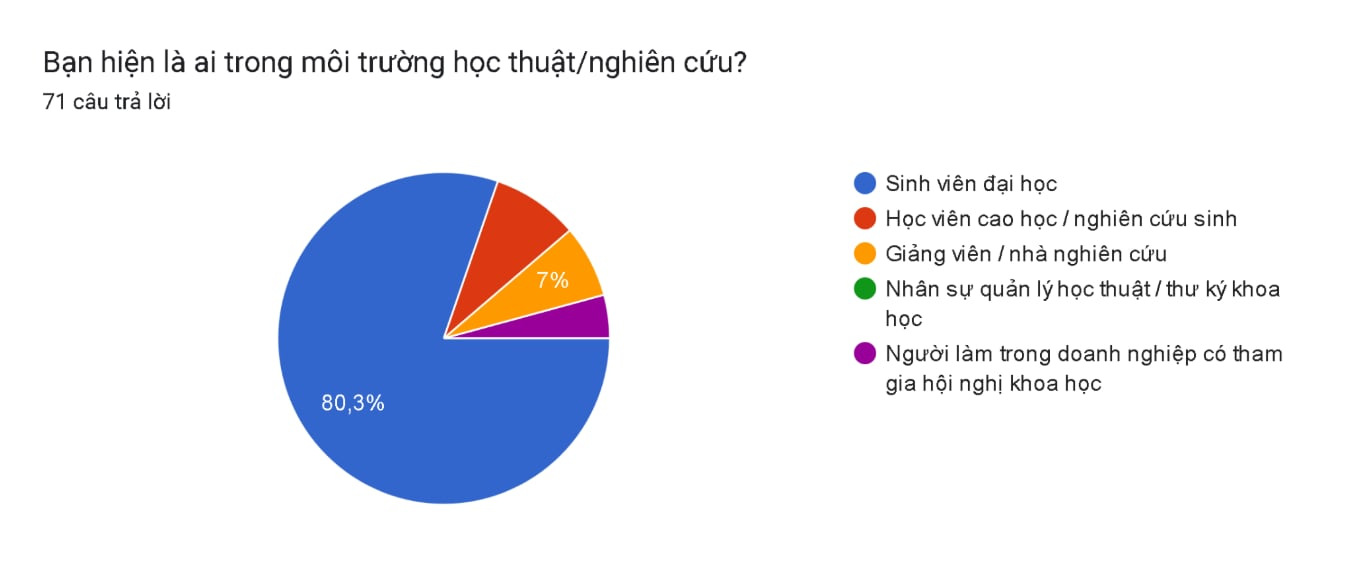
\includegraphics[width=0.9\textwidth]{images/chapter_2_picture_1.jpg}
    \caption{Phân bố đối tượng tham gia khảo sát}
    \label{fig:ch2-survey-participants}
\end{figure}

Hình~\ref{fig:ch2-survey-participants} trình bày phân bố mẫu khảo sát theo vai trò hoặc nhóm nghề nghiệp. Thành phần mẫu là cơ sở để xác định phạm vi diễn giải kết quả.

Trong phạm vi đề tài, ba nhóm vai trò được quan tâm nhất là:

\begin{itemize}
    \item \textbf{Tác giả:} người nộp bài, cần quy trình nộp bài dễ hiểu, giảm nhập liệu lặp lại, kiểm tra lỗi sớm và theo dõi trạng thái rõ ràng.
    \item \textbf{Phản biện viên:} người đọc và đánh giá bài báo, cần truy cập bài được phân công, nhanh chóng nắm được bối cảnh bài viết, viết nhận xét có chất lượng và giữ quyền tự quyết chuyên môn.
    \item \textbf{Chủ tọa/Đồng chủ tọa:} người có thẩm quyền cấu hình hội nghị, điều phối bài nộp, phân công phản biện viên, kiểm soát xung đột lợi ích và tổng hợp bằng chứng trước khi ra quyết định.
\end{itemize}

Cần lưu ý rằng số lượng phản hồi theo từng vai trò không đồng đều. Một số phân tích theo nhóm nhỏ như Chủ tọa hoặc Phản biện viên chỉ nên được đọc như tín hiệu định hướng, không phải kết luận thống kê đại diện cho toàn bộ cộng đồng học thuật.

\subsection{Phương pháp khảo sát}

Nhóm thực hiện khảo sát bằng biểu mẫu trực tuyến. Bộ câu hỏi gồm câu hỏi chọn một phương án, chọn nhiều phương án, câu hỏi theo thang Likert từ 1 đến 5 và câu hỏi mở. Cách thiết kế này vừa giúp lượng hóa mức độ phổ biến của các vấn đề, vừa thu thập lý do người dùng tin tưởng hoặc chưa tin tưởng các tính năng AI.

Các nhóm câu hỏi chính gồm:

\begin{itemize}
    \item Trải nghiệm với các nền tảng hiện có như EasyChair, Microsoft CMT và OpenReview.
    \item Các khó khăn thường gặp trong quy trình nộp bài, phản biện và quản lý hội nghị.
    \item Mức độ hữu ích của các tính năng dự kiến cho từng vai trò.
    \item Mức độ chấp nhận AI trong các tác vụ như tự động điền thông tin, kiểm tra sơ bộ bài nộp, hỗ trợ đọc bài, rà soát chất lượng phản biện và tổng hợp thông tin cho Chủ tọa.
\end{itemize}

Do khảo sát sử dụng mẫu thuận tiện, nhóm chỉ dùng kết quả để định hướng thiết kế và ưu tiên tính năng, không dùng để khẳng định xu hướng chung của toàn bộ cộng đồng nghiên cứu. Vì vậy, Chương 2 kết hợp dữ liệu khảo sát nội bộ với nguồn bên ngoài về áp lực xét duyệt học thuật và các hệ thống quản lý hội nghị hiện có.

\subsection{Kết quả khảo sát theo các vấn đề nổi bật}

Kết quả khảo sát cho thấy các khó khăn tập trung vào năm nhóm: thiếu chỉ dẫn về bước tiếp theo, biểu mẫu nhập liệu dài, phải đọc nhiều hướng dẫn dài, thiếu kiểm tra lỗi sớm, cùng tình trạng thông báo và hạn chót bị phân tán.

\begin{figure}[htbp]
    \centering
    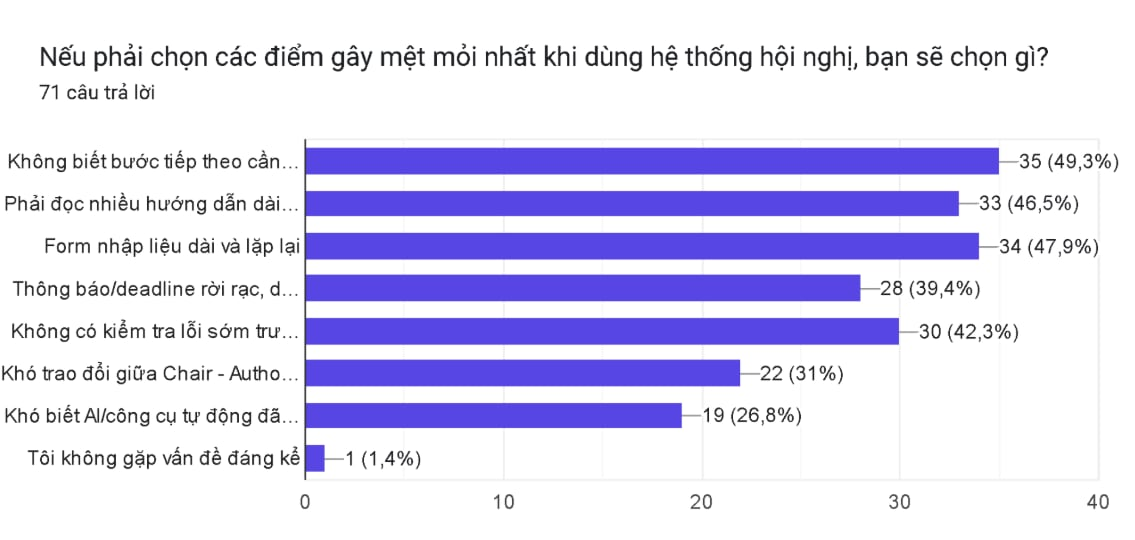
\includegraphics[width=0.9\textwidth]{images/chapter_2_picture_2.jpg}
    \caption{Các vấn đề người dùng gặp phải khi tham gia quy trình hội nghị khoa học}
    \label{fig:ch2-user-pain-points}
\end{figure}

Hình~\ref{fig:ch2-user-pain-points} minh họa phân bố các vấn đề nổi bật. Bảng dưới đây trình bày số liệu thu được từ khảo sát của nhóm.

\begin{center}
\small
\begin{tabular}{|P{0.23\textwidth}|P{0.23\textwidth}|P{0.23\textwidth}|P{0.23\textwidth}|}
\hline
Vấn đề nổi bật & Số người chọn & Tỷ lệ trên 71 phản hồi & Diễn giải thiết kế \\ \hline
Không biết bước tiếp theo cần làm là gì & 35 & 49,3\% & Hệ thống cần bảng điều khiển và lời nhắc hành động theo trạng thái, tránh để người dùng tự dò quy trình. \\ \hline
Biểu mẫu nhập liệu dài và lặp lại & 34 & 47,9\% & Quy trình nộp bài cần hỗ trợ trích xuất siêu dữ liệu từ tệp bài báo và cho phép người dùng chỉnh sửa trước khi gửi. \\ \hline
Phải đọc nhiều hướng dẫn dài trước khi thao tác & 33 & 46,5\% & Giao diện cần tổ chức thao tác theo từng bước, sử dụng ngôn ngữ rõ ràng và cung cấp trợ lý theo ngữ cảnh. \\ \hline
Không có kiểm tra lỗi sớm trước khi nộp chính thức & 30 & 42,3\% & Hệ thống cần kiểm tra sơ bộ trước khi bài nộp đi vào quy trình phản biện chính thức. \\ \hline
Thông báo và hạn chót bị phân tán, dễ bỏ sót & 28 & 39,4\% & Hệ thống cần tập trung thông báo và cập nhật trạng thái, thay vì phụ thuộc hoàn toàn vào thư điện tử. \\ \hline
\end{tabular}
\end{center}

Những số liệu này cho thấy khó khăn của người dùng không chỉ bắt nguồn từ việc thiếu chức năng nghiệp vụ. Nhiều hệ thống hiện có đã hỗ trợ nộp bài, phản biện và ra quyết định, nhưng quy trình thao tác vẫn phức tạp, phân tán và khó theo dõi. Vì vậy, ConferenceSpace không chỉ cần bao phủ các nghiệp vụ quản lý hội nghị mà còn phải giảm số bước và lượng thông tin người dùng phải nhập hoặc kiểm tra nhiều lần.

\subsection{Kết quả theo vai trò}

\subsubsection{a) Nhóm Chủ tọa/Ban tổ chức}

Trong nhóm người tham gia với vai trò Chủ tọa, các tính năng được quan tâm gồm cảnh báo xung đột lợi ích, bảng điều khiển trạng thái hội nghị và hỗ trợ phân công Phản biện viên. Tuy nhiên, số lượng Chủ tọa trong mẫu còn nhỏ nên các tỷ lệ của nhóm này chỉ có giá trị định hướng ưu tiên ban đầu.

\begin{center}
\small
\begin{tabular}{|P{0.31\textwidth}|P{0.31\textwidth}|P{0.31\textwidth}|}
\hline
Tính năng & Kết quả ghi nhận & Diễn giải \\ \hline
Cảnh báo xung đột lợi ích & 5/7 Chủ tọa đánh giá cao & Chủ tọa cần cơ chế cảnh báo sớm để tránh phân công sai người, nhưng kết quả cuối cùng vẫn cần người có thẩm quyền xác nhận. \\ \hline
Bảng điều khiển tóm tắt tình trạng hội nghị & 4/7 Chủ tọa đánh giá cao & Nhu cầu chính là giảm tải việc theo dõi thủ công qua nhiều bảng, thư điện tử và trang trạng thái rời rạc. \\ \hline
Gợi ý Phản biện viên theo chuyên môn & 2/7 Chủ tọa đánh giá cao & Tín hiệu này cho thấy Chủ tọa có thể thận trọng với việc tự động hóa phân công Phản biện viên; vì vậy, hệ thống nên trình bày gợi ý dưới dạng danh sách có điểm số và lý do rõ ràng, thay vì đưa ra quyết định tự động. \\ \hline
\end{tabular}
\end{center}

Tính năng đối sánh phản biện trong ConferenceSpace thuộc lớp thuật toán xác định, không phải luồng AI tạo sinh. Chủ tọa cần biết căn cứ xếp hạng phản biện viên, xung đột lợi ích nào đang ngăn việc phân công và có quyền ghi đè kết quả khi có căn cứ nghiệp vụ.

\subsubsection{b) Nhóm Tác giả}

Đối với Tác giả, nhu cầu nổi bật nhất là giảm lượng thông tin phải nhập trong quy trình nộp bài. Có 21 người chọn phương án ``tự điền và cho phép tôi sửa nhanh những mục sai'' cho chức năng Submission Autofill. Kết quả này cho thấy người dùng muốn hệ thống thực hiện các thao tác lặp lại nhưng không tự gửi bài thay họ; bước xác nhận vẫn thuộc trách nhiệm của Tác giả.

\begin{center}
\small
\begin{tabular}{|P{0.31\textwidth}|P{0.31\textwidth}|P{0.31\textwidth}|}
\hline
Tính năng & Kết quả ghi nhận & Diễn giải \\ \hline
Submission Autofill & Lựa chọn phổ biến nhất là tự điền nhưng cho phép sửa & Tính năng này nên tạo dữ liệu nháp, hiển thị các trường đã trích xuất và cho phép Tác giả chỉnh sửa. \\ \hline
Submission Gating & Người tham gia đánh giá tính năng này là hữu ích & Submission Gating nên cảnh báo lỗi sớm, nhưng không được tự động loại bài khi chưa có chính sách rõ ràng. \\ \hline
\end{tabular}
\end{center}

Xét về thiết kế, đây là nhóm tính năng ảnh hưởng trực tiếp nhất đến trải nghiệm ban đầu của Tác giả với hệ thống. Quy trình nộp bài cần giúp người dùng hoàn thành đúng yêu cầu, hiểu rõ trạng thái và sửa lỗi trước hạn chót.

\subsubsection{c) Nhóm Phản biện viên}

\begin{figure}[htbp]
    \centering
    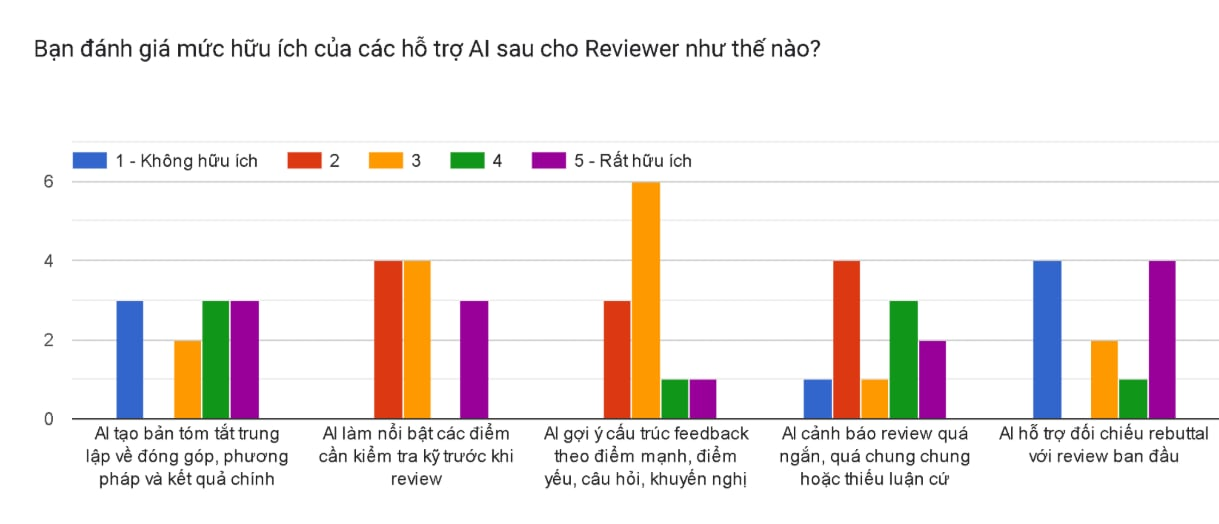
\includegraphics[width=0.9\textwidth]{images/chapter_2_picture_3.jpg}
    \caption{Mức độ ủng hộ AI của Phản biện viên theo từng tác vụ}
    \label{fig:ch2-reviewer-ai-acceptance}
\end{figure}

Hình~\ref{fig:ch2-reviewer-ai-acceptance} thể hiện mức độ chấp nhận AI của Phản biện viên theo từng tác vụ. Trong dữ liệu khảo sát, 6/11 Phản biện viên đánh giá cao tính năng dùng AI để tạo bản tóm tắt trung lập, trong khi chỉ 3/11 đánh giá cao tính năng dùng AI để nêu bật những điểm cần kiểm tra kỹ.

\begin{center}
\small
\begin{tabular}{|P{0.31\textwidth}|P{0.31\textwidth}|P{0.31\textwidth}|}
\hline
Tính năng & Kết quả ghi nhận & Diễn giải \\ \hline
Tóm tắt trung lập bài báo & 6/11 Phản biện viên đánh giá cao & AI có thể giúp Phản biện viên nắm bối cảnh ban đầu, nhưng bản tóm tắt không thay thế việc đọc bài. \\ \hline
Nêu bật điểm cần kiểm tra kỹ & 3/11 Phản biện viên đánh giá cao & Phản biện viên thận trọng với việc AI định hướng đánh giá học thuật; đầu ra nên là gợi ý kiểm tra, không phải kết luận chuyên môn. \\ \hline
\end{tabular}
\end{center}

Kết quả này phù hợp với các chính sách gần đây của những hội nghị lớn: AI có thể hỗ trợ Phản biện viên trong điều kiện được kiểm soát, nhưng Phản biện viên vẫn chịu trách nhiệm cuối cùng về nội dung bản phản biện, tính bảo mật của bản thảo và tính trung thực của đánh giá \cite{ch2ref15,ch2ref16}.

Do đó, AI chỉ nên hỗ trợ Phản biện viên định hướng việc đọc, không thay con người đọc và đánh giá bài báo. Khảo sát chưa đo khối lượng ghi chú, số lần đối chiếu hoặc thời gian rà soát; kết quả chỉ cho thấy người tham gia có xu hướng chấp nhận AI ở vai trò tạo bản tóm tắt và nêu những điểm cần kiểm tra.

\subsection{Diễn giải kết quả và giới hạn khảo sát}

Tổng hợp các phản hồi cho thấy bốn nhu cầu nền tảng:

\begin{enumerate}
    \item \textbf{Giảm thao tác thủ công:} người dùng muốn hệ thống xử lý phần nhập liệu và kiểm tra lặp lại, đặc biệt ở bước nộp bài.
    \item \textbf{Giảm tải nhận thức:} người dùng cần biết trạng thái hiện tại, việc tiếp theo cần làm và hạn chót liên quan mà không phải tự dò nhiều trang hoặc thư điện tử.
    \item \textbf{Tăng khả năng kiểm soát rủi ro:} Chủ tọa cần công cụ hỗ trợ phát hiện xung đột lợi ích và theo dõi tiến độ phản biện; Tác giả cần phát hiện lỗi trước khi gửi chính thức.
    \item \textbf{Bảo đảm tính minh bạch của AI:} người dùng chấp nhận AI khi công nghệ này chỉ đóng vai trò hỗ trợ, đưa ra kết quả có căn cứ và cho phép con người kiểm tra lại.
\end{enumerate}

Những kết luận này cần được diễn giải trong ba giới hạn. Thứ nhất, khảo sát sử dụng mẫu thuận tiện gồm 71 phản hồi nên không thể đại diện cho toàn bộ cộng đồng học thuật. Thứ hai, nhóm Chủ tọa và nhóm Phản biện viên có quy mô nhỏ; do đó, phân tích theo vai trò chỉ mang tính định hướng. Thứ ba, khảo sát này đo nhu cầu trước khi người tham gia sử dụng hệ thống, khác với khảo sát sau trải nghiệm được trình bày trong chương đánh giá.

\section{Khảo sát hiện trạng các hệ thống quản lý hội nghị}

\subsection{Đối tượng, tiêu chí và giới hạn khảo sát}

Nhóm chia các hệ thống khảo sát thành hai nhóm với mục đích đối chiếu khác nhau. Nhóm thứ nhất gồm EasyChair, HotCRP, OpenReview và Microsoft CMT. Các nền tảng này đã hoàn thiện quy trình nghiệp vụ và cung cấp chuẩn tham chiếu về vòng đời xét duyệt, vai trò, phân quyền, phân công, xung đột lợi ích, phản biện, phản hồi của tác giả và ra quyết định. Nhóm thứ hai gồm PeerSubmit, nền tảng lấy AI làm trọng tâm, và Morressier, đối tượng tham khảo bổ sung. PeerSubmit minh họa chiến lược đưa AI vào nhiều công đoạn của vòng đời; Morressier bổ sung góc nhìn về sàng lọc liêm chính, khai báo xung đột lợi ích và phân công phản biện có sự xác nhận của ban tổ chức.

Nhóm đối chiếu các nền tảng theo tám tiêu chí:

\begin{itemize}
    \item Mức bao phủ vòng đời xét duyệt và các vai trò được hỗ trợ;
    \item Các khâu tích hợp AI hoặc thuật toán trong vòng đời;
    \item Loại đầu ra được tạo và mức độ gần với quyết định học thuật;
    \item Cơ chế xác nhận, ghi đè hoặc chặn hành động;
    \item Khả năng giải thích, truy vết và kiểm tra lại kết quả;
    \item Phạm vi phân quyền đối với dữ liệu bài nộp và dữ liệu người dùng;
    \item Loại bằng chứng hỗ trợ cho từng nhận định;
    \item Các chức năng ngoài xét duyệt như đăng ký, thanh toán và trang thông tin sự kiện; tiêu chí này chỉ dùng để xác định phạm vi sản phẩm, không dùng để kết luận về chất lượng học thuật.
\end{itemize}

\subsection{Tổng quan các hệ thống hiện có}

\subsubsection{a) EasyChair}

EasyChair là hệ thống quản lý hội nghị có phạm vi sử dụng lớn theo số liệu do nhà cung cấp công bố. Trang chính thức của EasyChair nêu hơn 4,8 triệu người dùng và hơn 124.000 hội nghị đã sử dụng nền tảng này \cite{ch2ref1}. Hệ thống hỗ trợ nhiều thành phần của vòng đời hội nghị, bao gồm nộp bài, quản lý phản biện, quản lý quyền truy cập, xung đột lợi ích, phân công phản biện theo nguyện vọng, phản hồi của tác giả, thư điện tử, phân tích dữ liệu và xuất bản kỷ yếu \cite{ch2ref2}.

Bằng chứng từ cộng đồng hội nghị xác nhận EasyChair có thể vận hành một quy trình phản biện nhiều giai đoạn. ITiCSE 2025 sử dụng EasyChair cho phản biện kín hai chiều, đăng ký nguyện vọng phản biện, khai báo xung đột lợi ích, phân công bằng thuật toán, thảo luận và tổng hợp nhận xét của phản biện viên cấp cao \cite{ch2ref57}. Ở chiều ngược lại, một báo cáo kinh nghiệm công bố năm 2013 của thành viên ban tổ chức hội nghị ghi nhận rằng một số tùy chọn cấu hình khi đó khó tìm và phải thử nhiều lần mới hiểu, dù quy trình trở nên hữu ích sau khi người dùng đã làm quen \cite{ch2ref22}. Đây là một trường hợp sử dụng cụ thể, không đủ để kết luận EasyChair nhìn chung dễ hay khó sử dụng. Vì vậy, bài học phù hợp cho ConferenceSpace là tham khảo phạm vi quy trình của EasyChair, đồng thời đánh giá khả năng hướng dẫn theo ngữ cảnh bằng thử nghiệm người dùng của chính hệ thống thay vì suy diễn từ tài liệu hướng dẫn của EasyChair.

\subsubsection{b) HotCRP}

HotCRP hỗ trợ nhiều thành phần của quy trình phản biện và hoạt động điều phối của Chủ tọa. Theo tài liệu của HotCRP, hệ thống hỗ trợ phân công bài, đăng ký nguyện vọng phản biện, xung đột lợi ích, Chủ tọa ra quyết định, vai trò người điều phối thảo luận (lead), người hướng dẫn hoàn thiện bản sửa (shepherd), phân công tự động và chế độ chạy thử để kiểm tra kết quả trước khi áp dụng \cite{ch2ref3}. Tài liệu hướng dẫn dành cho Chủ tọa cũng mô tả cơ chế xử lý xung đột của Chủ tọa, quản trị viên phụ trách từng bài và có sử dụng cơ chế mã cấp quyền phản biện dùng để giới hạn quyền truy cập khi có xung đột \cite{ch2ref4}.

Báo cáo của hai đồng Chủ tọa chương trình USENIX ATC 2020 cung cấp bằng chứng vận hành cụ thể hơn. HotCRP hỗ trợ phân công hàng trăm bài cho hơn 100 thành viên ban chương trình; kết quả phân công tự động ban đầu được đánh giá là hữu ích nhưng vẫn cần Chủ tọa rà soát và điều chỉnh đáng kể. Báo cáo cũng ghi nhận danh mục chủ đề quá chi tiết làm tăng gánh nặng khai báo và có thể làm giảm chất lượng phân công ban đầu, trong khi cơ chế xung đột lợi ích ngăn thành viên có xung đột truy cập bài, điểm số và thảo luận liên quan \cite{ch2ref58}. Bằng chứng này xác nhận HotCRP đã được dùng để thực thi quy tắc truy cập và hỗ trợ Chủ tọa giám sát phân công, nhưng không chứng minh nền tảng chỉ phù hợp với người dùng có kinh nghiệm. ConferenceSpace vì vậy tham khảo nguyên tắc kiểm soát quyền và xác nhận phân công, còn mức độ dễ tiếp cận phải được đánh giá riêng trên người dùng của hệ thống.

\subsubsection{c) OpenReview}

OpenReview là nền tảng quản lý phản biện có khả năng cấu hình nhiều mức độ công khai. Trang giới thiệu chính thức mô tả đây là nền tảng đám mây cung cấp giao diện lập trình để truy cập dữ liệu theo quyền đọc và quyền ghi, hỗ trợ thảo luận mở, quản lý thông tin phục vụ xác định xung đột lợi ích và đối sánh bài báo với phản biện viên cho các hội nghị có hàng nghìn bài nộp \cite{ch2ref5}.

Các Chủ tọa chương trình NeurIPS 2021 đã chuyển toàn bộ quy trình sang OpenReview nhưng vẫn áp dụng phản biện kín hai chiều: trong thời gian xét duyệt, bài nộp chỉ hiển thị cho thành viên ban chương trình được phân công và các thảo luận nội bộ tiếp tục được giữ kín; chỉ bài được chấp nhận cùng các bản phản biện ẩn danh mới được công khai sau thời điểm thông báo \cite{ch2ref59}. Báo cáo sau hội nghị của các Chủ tọa chương trình ACT 2023 cũng cho thấy OpenReview phiên bản 1 có thể thích nghi với quy trình phản biện kín một chiều, nhưng một số xung đột lợi ích đặc thù, quyền xem thảo luận và việc thêm phản biện viên phụ vẫn cần cấu hình qua giao diện lập trình hoặc xử lý thủ công \cite{ch2ref60}. Vì vậy, điểm tham khảo có bằng chứng của OpenReview là khả năng cấu hình mức độ công khai và quyền truy cập; ConferenceSpace cần bảo đảm tính minh bạch có kiểm soát thay vì mặc định công khai toàn bộ quy trình.

\subsubsection{d) Microsoft CMT}

Microsoft CMT hỗ trợ nhiều vai trò, nhiều tiểu ban chuyên môn, toàn bộ vòng đời nộp bài, biểu mẫu tùy chỉnh, quản lý xung đột, đăng ký nguyện vọng phản biện, gợi ý phản biện viên, thảo luận, phản hồi của tác giả và phân công tích hợp với TPMS \cite{ch2ref6}. Tài liệu CMT về quản lý xung đột nêu hai cơ chế chính: xung đột theo cá nhân và xung đột theo miền thư điện tử; các xung đột này được xét trong quá trình phân công \cite{ch2ref7}. Theo tài liệu TPMS, điểm TPMS nằm trong khoảng từ 0 đến 1; điểm càng cao thì mức độ phù hợp giữa bài báo và phản biện viên càng lớn \cite{ch2ref8}.

Báo cáo của các Chủ tọa CVPR 2013 cho biết CMT đã quản lý toàn bộ quá trình nộp và xét duyệt 1.798 bài được phản biện đầy đủ. TPMS cung cấp gợi ý đối sánh; CMT chọn ba phản biện viên không có xung đột cho mỗi bài từ danh sách ứng viên; sau đó các Chủ tọa và Chủ tọa lĩnh vực vẫn thực hiện nhiều điều chỉnh thủ công để cải thiện mức độ phù hợp dưới ràng buộc về khối lượng công việc. Báo cáo kết luận trách nhiệm phân công thuộc về các Chủ tọa, còn CMT và TPMS đóng vai trò hỗ trợ \cite{ch2ref61}. Bằng chứng vận hành này củng cố cách ConferenceSpace thiết kế đối sánh như một chức năng hỗ trợ có thể kiểm tra, kết hợp điểm phù hợp chuyên môn, xung đột lợi ích, khối lượng công việc và quyền xác nhận của Chủ tọa, thay vì tự động ra quyết định cuối cùng.

\subsubsection{e) PeerSubmit: nền tảng lấy AI làm trọng tâm}

PeerSubmit tự định vị là nền tảng lấy AI làm trọng tâm trong quản lý bài nộp và xét duyệt. Tài liệu sản phẩm công bố một vòng đời chung gồm cấu hình hội nghị hoặc tạp chí, tiếp nhận bài, phân công phản biện viên, phản biện và ra quyết định. Nền tảng hỗ trợ nhiều tiểu ban chuyên môn, các chế độ phản biện kín một chiều, kín hai chiều và công khai, biểu mẫu chấm điểm, phản hồi của tác giả, nhiều vòng chỉnh sửa, phân quyền theo vai trò và nhật ký hoạt động \cite{ch2ref48}.

Danh mục chức năng AI trên trang sản phẩm gồm đối sánh phản biện theo chuyên môn kèm điểm tin cậy và kiểm tra xung đột lợi ích, tóm tắt bài nộp, sàng lọc chất lượng và mức độ phù hợp với phạm vi hội nghị, cùng bản tóm lược hỗ trợ quyết định (decision brief) tổng hợp điểm và nhận xét \cite{ch2ref48}. Bài viết kỹ thuật của nhà cung cấp mô tả phương pháp đối sánh bằng biểu diễn nhúng cho bài báo và hồ sơ phản biện viên, chỉ mục HNSW, truy vấn $K$ kết quả gần nhất, xếp hạng theo độ tương đồng cosine, sau đó lọc theo xung đột lợi ích và tình trạng sẵn sàng \cite{ch2ref53}. Đây là kiến trúc do nhà cung cấp mô tả; nguồn không công bố mô hình nhúng, dữ liệu đánh giá hoặc kết quả kiểm chứng độc lập, nên báo cáo không kết luận về việc triển khai thực tế hoặc chất lượng đối sánh.

Ranh giới trách nhiệm trong tài liệu PeerSubmit chưa hoàn toàn nhất quán. Trang sản phẩm mô tả Chủ tọa sử dụng bảng điều khiển quyết định để chấp nhận, từ chối hoặc yêu cầu sửa bài, còn bản tóm lược hỗ trợ quyết định chỉ tổng hợp điểm phản biện \cite{ch2ref48}. Bài viết về AI trong xét duyệt cũng khẳng định AI không đưa ra quyết định chấp nhận hoặc từ chối và phán đoán của con người vẫn giữ vai trò trung tâm \cite{ch2ref54}. Tuy nhiên, trang thông tin đồng thời quảng bá chức năng AI hỗ trợ chấm điểm bản phản biện và chức năng tạo phán quyết cuối cùng kèm điểm tin cậy \cite{ch2ref52}. Báo cáo xem sự khác biệt này là một giới hạn của tài liệu do nhà cung cấp công bố; nhóm không suy diễn rằng PeerSubmit hoàn toàn tự động ra quyết định, đồng thời không xem quyền ghi đè của con người là đặc điểm riêng của ConferenceSpace.

PeerSubmit tự công bố mức giảm 70\% đối với chu kỳ xét duyệt, 99\% đối với thời gian phân công và 40\% đối với thời gian phản biện, cùng tỷ lệ phù hợp giữa bài báo và phản biện viên là 96\% \cite{ch2ref48}. Trong phạm vi khảo sát, nhóm chưa tìm thấy báo cáo vận hành của một hội nghị, đánh giá cộng đồng hoặc nghiên cứu độc lập công bố dữ liệu nguồn, cỡ mẫu, tập tham chiếu, định nghĩa chỉ số và phương pháp đo tương ứng. Vì vậy, báo cáo chỉ xem các tỷ lệ này là tuyên bố của nhà cung cấp, không dùng làm kết quả thực nghiệm hoặc đường cơ sở cho ConferenceSpace. Tài liệu PeerSubmit cho thấy tự động hóa tại nhiều công đoạn là một chiến lược định vị sản phẩm. Do đó, câu hỏi có ý nghĩa đối với ConferenceSpace không còn là ``có tích hợp AI hay không'', mà là ``tác vụ nào nên dùng AI, tác vụ nào phải cho kết quả có thể tái tạo, ai xác nhận đầu ra và cần bằng chứng nào để đánh giá từng lựa chọn''.

\subsubsection{f) Morressier: tham khảo về liêm chính và phân công có xác nhận}

Morressier thể hiện một chiến lược khác: tích hợp kiểm tra đạo văn, trùng lặp hình ảnh và dấu hiệu của "cơ sở sản xuất bài báo hàng loạt" (paper mill) vào quy trình Integrity Manager để nhóm biên tập xem báo cáo trước khi ra quyết định \cite{ch2ref47}. Tài liệu Auto-Assign mô tả việc phân phối bài đều nhất có thể giữa các phản biện viên đã chấp nhận và tạo danh sách gợi ý để người tổ chức sửa trước khi xác nhận. Các điều kiện chặn được nêu cụ thể gồm phản biện viên đã được phân công cho bài, đã từ chối bài, là đồng tác giả của bài hoặc đã quá hạn phản biện \cite{ch2ref55}; phạm vi này không đủ để kết luận chức năng tự động phát hiện mọi dạng xung đột lợi ích. Từ phía cộng đồng xuất bản, IOP Publishing xác nhận đã hợp tác với Morressier để tích hợp luồng tiếp nhận, phản biện và xuất bản kỷ yếu cho các đơn vị tổ chức hội nghị mà IOP phục vụ \cite{ch2ref62}. Tuy nhiên, thông báo này được công bố năm 2021, trước khi Integrity Manager ra mắt, và không đánh giá Auto-Assign. Do đó, báo cáo chỉ dùng Morressier để tham khảo hai mẫu thiết kế cần được kiểm chứng thêm là sàng lọc liêm chính chuyên biệt và phân công có bước xác nhận, chứ không dùng làm bằng chứng về chất lượng hoặc hiệu quả của hai chức năng.

\subsection{So sánh phạm vi nghiệp vụ}

Bảng dưới đây xem xét liệu ConferenceSpace có đặt các thử nghiệm thuật toán và AI trong một vòng đời xét duyệt thống nhất hay chỉ ghép các luồng xử lý rời rạc. Mức hỗ trợ của các nền tảng đối chiếu được tổng hợp từ tài liệu công khai; cột ConferenceSpace chỉ mô tả phạm vi đề tài, không đánh giá chất lượng.

\begingroup
\small
\setlength{\tabcolsep}{2pt}
\setlength{\LTleft}{0pt}
\setlength{\LTright}{0pt}
\begin{longtable}{|P{0.17\textwidth}|P{0.20\textwidth}|P{0.20\textwidth}|P{0.20\textwidth}|P{0.17\textwidth}|}
  \caption{So sánh phạm vi nghiệp vụ của các nhóm nền tảng}\\
\hline
Nhóm nghiệp vụ & EasyChair/HotCRP & OpenReview/CMT & PeerSubmit & ConferenceSpace \\ \hline
\endfirsthead
\hline
Nhóm nghiệp vụ & EasyChair/HotCRP & OpenReview/CMT & PeerSubmit & ConferenceSpace \\ \hline
\endhead
\hline
\endfoot
Cấu hình hội nghị và chuyên đề & Có, với mức cấu hình khác nhau & Có & Có & Có trong phạm vi đề tài \\ \hline
Nộp bài, sửa bài và theo dõi trạng thái & Có & Có & Có & Có \\ \hline
Vai trò và phân quyền & Có & Có & Có, công bố cơ chế phân quyền theo vai trò & Có theo các vai trò Tác giả, Phản biện viên và Chủ tọa/Đồng chủ tọa \\ \hline
Phân công phản biện và xung đột lợi ích & Có cơ chế đăng ký nguyện vọng, ràng buộc hoặc khai báo xung đột & Có đối sánh, đăng ký nguyện vọng, TPMS và kiểm tra xung đột lợi ích & Có đối sánh kèm điểm tin cậy và kiểm tra xung đột lợi ích theo công bố của nhà cung cấp & Có thuật toán đối sánh xác định, cung cấp điểm và thông tin xung đột lợi ích để Chủ tọa xác nhận \\ \hline
Biểu mẫu, bản nháp và gửi bản phản biện & Có & Có & Có & Có \\ \hline
Phản hồi của tác giả, thảo luận và vòng chỉnh sửa & Có tùy cấu hình & Có & Có theo tài liệu sản phẩm & Có trong phạm vi luồng đã xây dựng \\ \hline
Quyết định và thông báo & Có & Có & Có bảng điều khiển quyết định và thư thông báo & Chủ tọa ra quyết định; hệ thống quản lý trạng thái và thông báo \\ \hline
Bản hoàn thiện sau chấp nhận & Có ở một số nền tảng & Có tùy quy trình & Có bước chấp nhận cuối cùng và công bố theo mô tả sản phẩm & Chỉ hỗ trợ tải lên và truy xuất tệp sau khi bài được chấp nhận; chưa có bước phê duyệt, thực thi hạn chót hoặc yêu cầu nộp lại \\ \hline
Đăng ký, thanh toán và trang thông tin sự kiện & Có ở một số gói hoặc qua tích hợp & Không phải trọng tâm chung & Có các chức năng sự kiện theo trang thông tin giá & Nằm ngoài phạm vi đề tài \\ \hline
\end{longtable}
\endgroup

Kết quả so sánh cho thấy ConferenceSpace tổ chức các thành phần nộp bài, phân công, xung đột lợi ích, phản biện, phản hồi của tác giả, ra quyết định và tải bản hoàn thiện sau chấp nhận trong cùng một mô hình trạng thái và quyền hạn. Vì vậy, các luồng hỗ trợ không phải những bản minh họa độc lập. Bảng chỉ xác nhận phạm vi đã xây dựng theo mô tả thiết kế, không xác nhận các chức năng vận hành đúng trong toàn bộ quy trình.

\subsection{So sánh với nền tảng có chiến lược lấy AI làm trọng tâm và quy ước trách nhiệm}

Bảng sau đối chiếu cách các nền tảng tích hợp cơ chế tự động hóa hoặc AI vào vòng đời xét duyệt. Mỗi ô mô tả quy ước được công bố về tác vụ, đầu ra và người xác nhận; bảng không nhằm xếp hạng chất lượng. Nội dung về PeerSubmit và Morressier dựa trên tuyên bố của nhà cung cấp, còn cột ConferenceSpace trình bày quy ước thiết kế. Mức độ triển khai và bằng chứng được đánh giá riêng ở Chương 4.

\begingroup
\small
\setlength{\tabcolsep}{2pt}
\setlength{\LTleft}{0pt}
\setlength{\LTright}{0pt}
\begin{longtable}{|P{0.16\textwidth}|P{0.24\textwidth}|P{0.27\textwidth}|P{0.27\textwidth}|}
  \caption{So sánh chiến lược AI và quy ước trách nhiệm}\\
\hline
Tác vụ & Nền tảng đã hoàn thiện nghiệp vụ/Morressier & PeerSubmit theo tài liệu nhà cung cấp & ConferenceSpace \\ \hline
\endfirsthead
\hline
Tác vụ & Nền tảng đã hoàn thiện nghiệp vụ/Morressier & PeerSubmit theo tài liệu nhà cung cấp & ConferenceSpace \\ \hline
\endhead
\hline
\endfoot
Nhập liệu và sàng lọc & Các nền tảng đã hoàn thiện nghiệp vụ sử dụng biểu mẫu; Morressier công bố chức năng kiểm tra trước khi nộp và kiểm tra liêm chính chuyên biệt & Công bố chức năng sàng lọc chất lượng và mức độ phù hợp với phạm vi hội nghị, trích xuất chủ đề và từ khóa & Submission Autofill tạo bản nháp để Tác giả sửa và xác nhận; Submission Gating tách lỗi theo quy tắc khỏi cảnh báo về nội dung do AI phát hiện \\ \hline
Đối sánh phản biện & CMT sử dụng TPMS; Morressier phân công tự động theo chủ đề, tải và xung đột, sau đó người tổ chức xác nhận & Sử dụng biểu diễn nhúng, HNSW, truy vấn $K$ kết quả gần nhất, độ tương đồng cosin và bộ lọc xung đột lợi ích; Chủ tọa có thể phê duyệt hoặc ghi đè gợi ý & Sử dụng Jaccard cùng ràng buộc về khối lượng công việc và xung đột lợi ích để cho kết quả xác định; Chủ tọa xác nhận hoặc ghi đè quyết định \\ \hline
Phát hiện xung đột lợi ích & Nhiều nền tảng có cơ chế khai báo hoặc quy tắc xung đột; Morressier chặn một số trường hợp phân công & Công bố chức năng tự động kiểm tra xung đột lợi ích trong quá trình đối sánh & Kết hợp tự kiểm tra, khai báo và đồ thị đồng tác giả; hiển thị bằng chứng nhưng không tuyên bố phát hiện đầy đủ \\ \hline
Tóm tắt bài nộp & Không phải năng lực cốt lõi chung của nhóm nền tảng đã hoàn thiện nghiệp vụ & Công bố chức năng tóm tắt phương pháp, đóng góp và cảnh báo các vấn đề về chất lượng & Reviewer Initial Analysis tạo bản tóm tắt, nêu điểm mạnh, điểm yếu, gợi ý; không tự điền, gửi, chấm điểm hoặc đưa ra khuyến nghị cuối cùng trong biểu mẫu phản biện \\ \hline
Rà soát bản phản biện & Sử dụng biểu mẫu và quy tắc nghiệp vụ; Morressier tập trung vào tính liêm chính của bài nộp & Trang thông tin giá công bố chức năng AI hỗ trợ chấm điểm bản phản biện và phát hiện nội dung không nhất quán & Review Quality Auditor rà soát bản phản biện nháp trước khi gửi để  \\ \hline
Tổng hợp thông tin trước quyết định & Cung cấp bảng điểm, thảo luận và chức năng ra quyết định của Chủ tọa tùy nền tảng & Công bố bản tóm lược hỗ trợ quyết định; trang thông tin giá còn quảng bá chức năng tạo phán quyết cuối cùng, trong khi bài viết khác vẫn giao quyền chấp nhận hoặc từ chối cho con người & Chair Decision Copilot tổng hợp bằng chứng và bất đồng; chức năng này không tạo phán quyết chấp nhận hoặc từ chối bài báo \\ \hline
Trợ lý cho nhiều vai trò & Chưa ghi nhận đây là năng lực cốt lõi chung & Chưa đủ tài liệu công khai để kết luận về quy ước truy cập tài nguyên theo từng vai trò & Chatbot Agent chỉ gọi công cụ trong phạm vi quyền và từ chối yêu cầu ngoài phạm vi, ngoài quyền truy cập \\ \hline
Loại bằng chứng & Tài liệu sản phẩm và hỗ trợ; một số cơ chế có nghiên cứu riêng & Chủ yếu là tài liệu và số liệu do nhà cung cấp công bố; nhóm chưa xác nhận được đánh giá độc lập & Mã nguồn, kết quả kiểm thử, đánh giá theo tác vụ và kiểm thử chấp nhận của người dùng ở Chương 4; mức độ bằng chứng khác nhau giữa các luồng \\ \hline
\end{longtable}
\endgroup


\subsection{Đối chiếu kết quả khảo sát với bằng chứng bên ngoài và chính sách học thuật}

Khảo sát nhu cầu sử dụng mẫu thuận tiện, trong đó số người tham gia với vai trò Chủ tọa và Phản biện viên còn nhỏ. Vì vậy, nhóm đối chiếu các nguyên tắc rút ra từ khảo sát với nguồn bên ngoài để kiểm tra tính phù hợp với thực tiễn vận hành và chính sách học thuật. Bước đối chiếu này không nhằm ước lượng tỷ lệ nhu cầu trong toàn bộ cộng đồng, xác lập khoảng trống thị trường hoặc chứng minh hiệu quả của ConferenceSpace.

Nhóm phân biệt bốn loại nguồn theo phạm vi có thể kết luận. Tài liệu sản phẩm chỉ xác nhận chức năng được công bố; báo cáo của Chủ tọa hoặc ban chương trình cung cấp bằng chứng về cách một hội nghị cụ thể đã vận hành; chính sách của hội nghị, hiệp hội và nhà xuất bản xác định trách nhiệm cùng giới hạn sử dụng AI; nghiên cứu có công bố phương pháp cung cấp bằng chứng thực nghiệm trong phạm vi mẫu và thiết kế nghiên cứu. Nhóm ưu tiên nguồn chính thức và nghiên cứu gốc, đồng thời giữ lại các trường hợp khác biệt giữa chính sách thay vì xem một quy định đơn lẻ là đồng thuận của toàn cộng đồng.

Đối với phân công phản biện, các báo cáo vận hành củng cố yêu cầu kết hợp thuật toán với quyền kiểm soát của con người. Tại USENIX ATC 2020, kết quả phân công ban đầu của HotCRP được các đồng Chủ tọa đánh giá là hữu ích nhưng vẫn cần rà soát và điều chỉnh đáng kể \cite{ch2ref58}. Tại CVPR 2013, TPMS cung cấp kết quả đối sánh, CMT chọn các Phản biện viên không có xung đột từ danh sách ứng viên, sau đó Chủ tọa và Chủ tọa lĩnh vực tiếp tục điều chỉnh dưới ràng buộc về khối lượng công việc \cite{ch2ref61}. Hai trường hợp không chứng minh một thuật toán cụ thể tốt hơn các phương pháp khác, nhưng xác nhận rằng điểm phù hợp, xung đột lợi ích, khối lượng công việc và bước xác nhận là các thành phần riêng biệt của quy trình phân công.

Yêu cầu phát hiện xung đột lợi ích qua nhiều nguồn cũng phù hợp với chính sách học thuật. ACM quy định người tham gia phải khai báo xung đột tiềm ẩn, nhưng đồng thời nhấn mạnh một chính sách đáng tin cậy không thể chỉ dựa vào việc mỗi cá nhân tự xác định xung đột của mình; người phụ trách như Chủ tọa hoặc biên tập viên vẫn phải đánh giá và xử lý trường hợp được báo cáo \cite{ch2ref12}. Do đó, kết quả từ quy tắc, đồ thị đồng tác giả hoặc dữ liệu học thuật bên ngoài trong ConferenceSpace chỉ nên được trình bày như bằng chứng hỗ trợ để Chủ tọa xem xét, không phải kết luận tự động rằng một cặp bài báo-Phản biện viên chắc chắn có hoặc không có xung đột.

Nhu cầu kiểm tra liêm chính có bằng chứng khảo sát bên ngoài, nhưng phạm vi trách nhiệm còn chưa thống nhất. Nghiên cứu của Calamur và Ghosh phân tích khảo sát năm 2022 với 852 người tham gia; sau khi loại 22 người không đồng ý tham gia và 145 người không trả lời câu hỏi nào, phân tích còn 685 phiếu có dữ liệu. Trong 401 người từng thực hiện phản biện, 174 người (43,39\%) cho biết đã gặp bản thảo bị nghi ngờ vi phạm liêm chính; 540 người trong mẫu phân tích (78,83\%) kỳ vọng quy trình phản biện có khả năng nhận diện đạo văn \cite{ch2ref56}. Các tác giả đồng thời đặt vấn đề liệu trách nhiệm này thuộc về Phản biện viên, nhóm biên tập hay công cụ chuyên biệt. Vì vậy, các tỷ lệ trên củng cố nhu cầu có bước sàng lọc và chuyển bằng chứng cho người có thẩm quyền, nhưng không chứng minh AI có thể tự xác định hành vi vi phạm.

Các chính sách AI được khảo sát hội tụ ở hai yêu cầu: bảo mật bản thảo và giữ trách nhiệm ở con người; tuy nhiên, phạm vi sử dụng được phép khác nhau đáng kể. ICLR 2026 cho phép dùng mô hình ngôn ngữ lớn để cải thiện ngữ pháp và độ rõ của bản phản biện nếu khai báo, nhưng Phản biện viên vẫn chịu trách nhiệm về nội dung và không được vi phạm tính bảo mật của bài chưa công bố \cite{ch2ref15}. Ngược lại, ICML 2025 cấm Phản biện viên dùng AI tạo sinh để viết bản phản biện hoặc đưa bất kỳ nội dung nào của bài nộp hay bản phản biện vào công cụ AI tạo sinh \cite{ch2ref16}. ACM cho phép dùng công cụ để cải thiện văn bản do Phản biện viên viết nếu trước đó đã loại toàn bộ thông tin có thể nhận diện bài nộp, Tác giả và Phản biện viên. ACM cũng cho phép dùng hệ thống có cam kết duy trì tính bảo mật của thông tin được tải lên; trong cả hai trường hợp, Phản biện viên vẫn chịu trách nhiệm về thiên lệch và nội dung được tạo \cite{ch2ref40}. Nature Portfolio yêu cầu Phản biện viên không tải bản thảo lên công cụ AI tạo sinh và phải khai báo nếu AI hỗ trợ bất kỳ phần nào của việc đánh giá các tuyên bố trong bài \cite{ch2ref41}. Sự khác biệt này cho thấy chức năng AI cho Phản biện viên phải có khả năng bật, tắt hoặc giới hạn theo chính sách của từng hội nghị; một cấu hình chung không thể mặc nhiên phù hợp với mọi nơi.

Bằng chứng thực nghiệm hiện có cũng ủng hộ cách tiếp cận thử nghiệm có kiểm soát thay vì giả định AI luôn cải thiện phản biện. Tại ICLR 2025, Review Feedback Agent chỉ cung cấp góp ý tùy chọn trên bản phản biện do con người đã viết và không trực tiếp sửa nội dung. Trong thử nghiệm ngẫu nhiên quy mô lớn, 26,6\% Phản biện viên nhận góp ý đã cập nhật bản phản biện; nhóm nghiên cứu còn báo cáo bản phản biện được sửa dài hơn và được đánh giá cao hơn trong phép đánh giá mù, nhưng thừa nhận cần tiếp tục nghiên cứu giới hạn của phản hồi do AI tạo \cite{ch2ref17,ch2ref18}. NeurIPS 2026 tiếp tục khảo sát một phạm vi rộng hơn bằng thử nghiệm tự nguyện: Tác giả và Phản biện viên phải đồng ý tham gia, các phân công được chia ngẫu nhiên giữa điều kiện không dùng AI và hai điều kiện hỗ trợ, dữ liệu không được nhà cung cấp lưu giữ, còn Chủ tọa lĩnh vực đánh giá bản phản biện mà không biết điều kiện thử nghiệm. Công cụ được định vị để hỗ trợ hiểu và phân tích bài, không viết bản phản biện hoặc thay thế phán đoán của Phản biện viên \cite{ch2ref19}. Vì thử nghiệm NeurIPS chưa công bố kết quả tại thời điểm khảo sát, báo cáo chỉ dùng thiết kế này làm tham chiếu về biện pháp kiểm soát, không dùng làm bằng chứng về hiệu quả.

Việc đối chiếu vì vậy củng cố ba yêu cầu cho ConferenceSpace: phân công và phát hiện xung đột lợi ích phải cung cấp căn cứ để Chủ tọa xác nhận; chức năng AI phải tuân theo chính sách bảo mật và trách nhiệm của từng hội nghị; hiệu quả của mỗi luồng AI phải được đo riêng trong điều kiện sử dụng xác định. Các nhu cầu về giảm nhập liệu, chỉ dẫn bước tiếp theo và thông báo tập trung vẫn chủ yếu bắt nguồn từ khảo sát nội bộ và không được khái quát bằng các nguồn bên ngoài nêu trên. Chương 4 đánh giá mức độ đáp ứng của ConferenceSpace trong phạm vi dữ liệu, phép thử và kiểm thử chấp nhận của người dùng đã thực hiện.

\section{Vấn đề thực tiễn và nguyên tắc giải pháp}

\subsection{Các vấn đề thiết kế rút ra từ khảo sát}

Các nền tảng đã hoàn thiện phần lớn nghiệp vụ cốt lõi, còn PeerSubmit và Morressier cho thấy AI hoặc cơ chế tự động hóa đã xuất hiện ở nhiều công đoạn. Vì vậy, vấn đề của đề tài không còn là thị trường ``thiếu AI tích hợp'', mà là cách xử lý các tác vụ khác nhau về mức độ nghiêm trọng của hậu quả, yêu cầu đối với tính ổn định và chủ thể chịu trách nhiệm. Từ đó, nhóm xác định năm vấn đề thiết kế.

\textbf{Thứ nhất, giảm nhập liệu không được loại bỏ bước xác nhận của Tác giả.} Gần một nửa số người tham gia khảo sát chọn biểu mẫu dài và lặp lại là vấn đề nổi bật. Submission Autofill có thể tạo siêu dữ liệu nháp, nhưng Tác giả phải có quyền sửa từng trường và quyết định thời điểm gửi bài.

\textbf{Thứ hai, đối sánh phản biện và phát hiện xung đột lợi ích cần cho kết quả ổn định, có căn cứ.} TPMS, PeerSubmit và Morressier cho thấy nhiều chiến lược đối sánh đã được triển khai \cite{ch2ref8,ch2ref53,ch2ref55}. Tuy nhiên, phân công sai có thể ảnh hưởng đến tính công bằng và bảo mật. Vì vậy, ConferenceSpace sử dụng thuật toán xác định, hiển thị điểm số, lý do và ràng buộc, sau đó để Chủ tọa xác nhận. Lựa chọn này không hàm ý Domain Jaccard tốt hơn phương pháp đối sánh theo ngữ nghĩa.

\textbf{Thứ ba, nội dung hỗ trợ đọc và tổng hợp phải bám sát bằng chứng, đồng thời đi kèm phân tích.} Tóm tắt, cảnh báo hoặc nội dung tổng hợp có thể giảm tải nhận thức, nhưng đầu ra không cố định có thể bỏ sót thông tin, suy diễn thiếu căn cứ hoặc gây nhiễu. Mỗi luồng cần được đánh giá bằng chỉ số riêng, có phân tích các trường hợp sai và chỉ được kết luận trong phạm vi dữ liệu đã đo.

\textbf{Thứ tư, các luồng xử lý gần bước ra quyết định phải công khai mức độ ảnh hưởng đến quyền tác giả của Phản biện viên và phán quyết học thuật.} Chính sách ICLR yêu cầu người tham gia chịu trách nhiệm về nội dung của mình; ICML cấm Phản biện viên dùng AI tạo sinh để viết bản phản biện hoặc đưa nội dung mật vào công cụ AI \cite{ch2ref15,ch2ref16}. Nghiên cứu Review Feedback Agent chỉ hỗ trợ góp ý trên bản nháp do con người viết \cite{ch2ref17,ch2ref18}. ConferenceSpace không cho phép AI tự điền hoặc gửi biểu mẫu, chấm điểm hay tạo phán quyết chấp nhận hoặc từ chối.

\textbf{Thứ năm, trợ lý phục vụ nhiều vai trò phải giữ đúng ranh giới truy cập tài nguyên.} Chatbot Agent chỉ được truy vấn dữ liệu mà người dùng hiện tại có quyền xem; hệ thống phải từ chối yêu cầu ngoài phạm vi thay vì trả lời bằng suy đoán. Cơ chế phân quyền ở cấp ứng dụng không có nghĩa là hệ thống đã kiểm toán toàn bộ vòng đời lưu giữ, sử dụng để huấn luyện hoặc vị trí lưu trữ dữ liệu của nhà cung cấp AI.

Mô hình ba lớp là lựa chọn thiết kế để xử lý năm vấn đề trên: lớp nghiệp vụ cốt lõi quản lý trạng thái và quyền hạn; lớp thuật toán xác định và có thể kiểm chứng xử lý đối sánh, xung đột lợi ích và các quy tắc; lớp AI hỗ trợ có kiểm soát tạo bản nháp, phân tích, cảnh báo hoặc tổng hợp. Báo cáo không xem mô hình này là điểm mới của thị trường hay kiến trúc tối ưu duy nhất.

\subsection{Liên kết vấn đề với định hướng giải pháp}

ConferenceSpace được thiết kế để xử lý năm vấn đề trên trong phạm vi một vòng đời xét duyệt chung. Bảng sau liên kết từng vấn đề với chức năng liên quan và ranh giới trách nhiệm; mối liên kết này giải thích lựa chọn thiết kế, không thay thế bằng chứng đánh giá ở Chương 4.

\begingroup
\small
\setlength{\tabcolsep}{2pt}
\setlength{\LTleft}{0pt}
\setlength{\LTright}{0pt}
\begin{longtable}{|P{0.31\textwidth}|P{0.31\textwidth}|P{0.31\textwidth}|}
  \caption{Liên kết vấn đề thiết kế với định hướng giải pháp ConferenceSpace}\\
\hline
Vấn đề thiết kế & Định hướng trong ConferenceSpace & Ranh giới trách nhiệm \\ \hline
\endfirsthead
\hline
Vấn đề thiết kế & Định hướng trong ConferenceSpace & Ranh giới trách nhiệm \\ \hline
\endhead
\hline
\endfoot
Nộp bài thủ công, biểu mẫu dài & Submission Autofill trích xuất siêu dữ liệu từ tệp PDF và gợi ý chuyên đề trong phạm vi hội nghị & Đầu ra là bản nháp có thể chỉnh sửa; Tác giả xác nhận trước khi gửi \\ \hline
Thiếu kiểm tra lỗi sớm & Submission Gating kiểm tra các điều kiện cơ bản trước khi bài nộp đi vào quy trình phản biện & Cảnh báo hoặc chặn theo chính sách đã cấu hình; không tự động loại bài ngoài các quy tắc của hệ thống \\ \hline
Khó kiểm soát việc đối sánh phản biện và xung đột lợi ích & Thuật toán đối sánh cung cấp điểm số và kết hợp nhiều lớp phát hiện xung đột lợi ích & Đối sánh phản biện thuộc lớp thuật toán xác định; Chủ tọa ra quyết định cuối cùng \\ \hline
Phản biện viên thiếu công cụ hỗ trợ đọc hiểu ban đầu và phải tự ghi chú nhiều điểm cần kiểm tra & Reviewer Initial Analysis cung cấp bản tóm tắt, các điểm cần kiểm tra và căn cứ liên quan & AI hỗ trợ định hướng đọc; khảo sát chưa đo mức giảm thao tác, thời gian rà soát hoặc ảnh hưởng đến đánh giá chuyên môn \\ \hline
Phản biện viên cần hỗ trợ rà soát bản nháp; Chủ tọa khó tổng hợp nhiều bản phản biện và phản hồi của tác giả & Review Quality Auditor cảnh báo vấn đề trong bản nháp; Chair Decision Copilot tổng hợp điểm đồng thuận, bất đồng và rủi ro & Không tự động sửa hoặc gửi bản phản biện, cũng không tạo quyết định chấp nhận hoặc từ chối; chỉ cung cấp thông tin để người có thẩm quyền xem xét \\ \hline
Người dùng khó tìm hướng dẫn thao tác & Chatbot Agent truy vấn dữ liệu hệ thống trong phạm vi quyền truy cập & Câu trả lời phải bám dữ liệu hệ thống và không vượt quá quyền của người dùng \\ \hline
Thông báo và trạng thái phân tán & Bảng điều khiển và thông báo trong hệ thống & Tập trung trạng thái và giảm phụ thuộc vào thư điện tử \\ \hline
\end{longtable}
\endgroup

Mối liên hệ này ngăn các chức năng AI trở thành phần bổ sung không gắn với nhu cầu. Trong ConferenceSpace, mỗi luồng AI phải xử lý một vấn đề cụ thể, dừng trước hành động thuộc trách nhiệm con người và được đánh giá riêng ở Chương 4.

\subsection{Nguyên tắc thiết kế từ các vấn đề đã xác định}

Từ phân tích trên, nhóm xác định bốn nguyên tắc thiết kế cho ConferenceSpace.

\textbf{Nguyên tắc 1: Tách lớp nghiệp vụ cốt lõi, thuật toán xác định và AI hỗ trợ.} Hệ thống không giao các hoạt động nộp bài, phân công, phản biện và ra quyết định cho AI tạo sinh. Đối sánh phản biện và phát hiện xung đột lợi ích thuộc lớp thuật toán xác định vì cần bảo đảm tính nhất quán, khả năng giải thích và khả năng kiểm tra. AI chỉ tham gia các tác vụ trích xuất, tóm tắt, rà soát và tổng hợp. Thiết kế cung cấp luồng thao tác thủ công khi không dùng AI.

\textbf{Nguyên tắc 2: Con người giữ quyền quyết định học thuật và quyền thực hiện hành động nghiệp vụ.} AI không quyết định chấp nhận hay từ chối bài, không tự phân công Phản biện viên và không chấm điểm thay Phản biện viên. Kết quả do AI tạo chỉ được dùng để cảnh báo; chỉ các quy tắc xác định đối với trường bắt buộc hoặc trạng thái nghiệp vụ mới được phép chặn thao tác. Review Quality Auditor hiện chưa tuân thủ phần sau của nguyên tắc này vì kết quả cảnh báo nghiêm trọng có thể ngăn thao tác gửi nhưng chưa cho phép người dùng ghi đè. Chương 4 phải đánh giá ranh giới này là chưa đáp ứng, thay vì xem đây là cơ chế kiểm soát hoàn thiện của con người.

\textbf{Nguyên tắc 3: Mọi gợi ý quan trọng cần có căn cứ.} Gợi ý Phản biện viên cần kèm điểm phù hợp và lý do; cảnh báo xung đột lợi ích cần nêu quan hệ hoặc nguồn dữ liệu; Chair Decision Copilot cần chỉ ra bản phản biện hoặc phản hồi nào là căn cứ của nhận định tổng hợp. Đây là điều kiện để người dùng có thể đánh giá, kiểm tra và ghi đè kết quả.

\textbf{Nguyên tắc 4: Đánh giá AI theo đúng bản chất từng luồng xử lý.} Các luồng tạo dữ liệu nháp, kiểm tra sơ bộ, hỗ trợ đọc hiểu và tổng hợp bằng chứng cần được đánh giá bằng tiêu chí khác nhau. Nguyên tắc này giúp chương đánh giá về sau tránh dùng một thước đo chung cho mọi đầu ra AI hoặc diễn giải quá mức vai trò của hệ thống.

\section{Tổng hợp yêu cầu hệ thống từ khảo sát}

Mục 2.4 chuyển kết quả khảo sát và các vấn đề thiết kế thành yêu cầu hệ thống. Đây là điểm nối giữa Chương 2 và Chương 3: mỗi nhóm yêu cầu dưới đây bắt nguồn từ nhu cầu người dùng, chuẩn nghiệp vụ, xu hướng lấy AI làm trọng tâm hoặc nguyên tắc trách nhiệm đã phân tích ở trên.

\subsection{Yêu cầu chức năng theo vai trò}

\subsubsection{a) Yêu cầu cho Tác giả}

\begingroup
\small
\setlength{\tabcolsep}{2pt}
\setlength{\LTleft}{0pt}
\setlength{\LTright}{0pt}
\begin{longtable}{|P{0.31\textwidth}|P{0.31\textwidth}|P{0.31\textwidth}|}
  \caption{Yêu cầu chức năng dành cho Tác giả}\\
\hline
Mã & Yêu cầu & Cơ sở \\ \hline
\endfirsthead
\hline
Mã & Yêu cầu & Cơ sở \\ \hline
\endhead
\hline
\endfoot
F-AUTHOR-01 & Tác giả có thể tìm kiếm và xem thông tin về hội nghị, chuyên đề, hạn chót và lời mời nộp bài (CFP). & Nhu cầu theo dõi tập trung hạn chót và trạng thái. \\ \hline
F-AUTHOR-02 & Tác giả có thể nộp bài theo quy trình nhiều bước gồm khai báo thông tin bài báo, tác giả, tệp, xung đột lợi ích, xem lại và gửi. & Các hệ thống hiện có đều chuẩn hóa vòng đời nộp bài; ConferenceSpace cần bao phủ nghiệp vụ cốt lõi. \\ \hline
F-AUTHOR-03 & Submission Autofill hỗ trợ trích xuất siêu dữ liệu từ bản thảo PDF, gồm tiêu đề, tóm tắt, tác giả, cơ quan công tác, địa chỉ thư điện tử và từ khóa khi có thể. & Vấn đề nổi bật là biểu mẫu nhập liệu dài và lặp lại. \\ \hline
F-AUTHOR-04 & Submission Autofill gợi ý chuyên đề dựa trên danh sách chuyên đề đang hoạt động của hội nghị và siêu dữ liệu bài nộp. & Nhu cầu giảm thao tác chọn chuyên đề; gợi ý này hiện là một đầu ra của Submission Autofill. \\ \hline
F-AUTHOR-05 & Hệ thống kiểm tra sơ bộ bài nộp trước khi gửi chính thức và hiển thị các lỗi hoặc cảnh báo mà Tác giả có thể xử lý. & Vấn đề nổi bật là thiếu kiểm tra lỗi sớm. \\ \hline
F-AUTHOR-06 & Tác giả có thể lưu bản nháp, chỉnh sửa trước hạn chót, rút bài, xem bản phản biện, gửi phản hồi và tải bản hoàn thiện sau khi bài được chấp nhận. Luồng xử lý bản hoàn thiện chưa có bước phê duyệt, thực thi hạn chót hoặc yêu cầu nộp lại. & Yêu cầu nghiệp vụ của vòng đời xét duyệt; chức năng xử lý bản hoàn thiện mới được xây dựng một phần. \\ \hline
\end{longtable}
\endgroup

\subsubsection{b) Yêu cầu cho Phản biện viên}

\begin{table}[H]
\centering
\caption{Yêu cầu chức năng dành cho Phản biện viên}
\small
\begin{tabular}{|P{0.31\textwidth}|P{0.31\textwidth}|P{0.31\textwidth}|}
\hline
Mã & Yêu cầu & Cơ sở \\ \hline
F-REVIEWER-01 & Phản biện viên có thể chấp nhận hoặc từ chối lời mời và xem danh sách bài được phân công. & Nghiệp vụ phản biện cơ bản. \\ \hline
F-REVIEWER-02 & Phản biện viên có thể xem bài báo, tệp, siêu dữ liệu, hạn chót và trạng thái phản biện. & Nhu cầu biết rõ bước tiếp theo trong quy trình. \\ \hline
F-REVIEWER-03 & Phản biện viên có thể nhập điểm, nhận xét và mức độ tự tin, đồng thời lưu bản nháp và gửi bản phản biện chính thức. & Nghiệp vụ phản biện. \\ \hline
F-REVIEWER-04 & Hệ thống có thể cung cấp bản tóm tắt, các điểm cần kiểm tra và căn cứ liên quan để hỗ trợ bước đọc ban đầu. & Phản biện viên trong khảo sát có xu hướng chấp nhận AI ở vai trò hỗ trợ đọc; khảo sát chưa đo mức giảm thao tác hoặc thời gian rà soát. \\ \hline
F-REVIEWER-05 & AI không tự điền hoặc gửi biểu mẫu, chấm điểm hay đưa ra khuyến nghị cuối cùng. Reviewer Initial Analysis vẫn tạo nội dung có thể ảnh hưởng đến nhận định và chỉ được bật khi chính sách hội nghị cho phép. & Giới hạn các hành động thuộc trách nhiệm của Phản biện viên và công khai giới hạn chính sách của nội dung hỗ trợ \cite{ch2ref15,ch2ref16}. \\ \hline
\end{tabular}
\end{table}

\subsubsection{c) Yêu cầu cho Chủ tọa/Ban tổ chức}

\begingroup
\small
\setlength{\tabcolsep}{2pt}
\setlength{\LTleft}{0pt}
\setlength{\LTright}{0pt}
\begin{longtable}{|P{0.31\textwidth}|P{0.31\textwidth}|P{0.31\textwidth}|}
  \caption{Yêu cầu chức năng dành cho Chủ tọa và Ban tổ chức}\\
\hline
Mã & Yêu cầu & Cơ sở \\ \hline
\endfirsthead
\hline
Mã & Yêu cầu & Cơ sở \\ \hline
\endhead
\hline
\endfoot
F-CHAIR-01 & Chủ tọa có thể tạo và cấu hình hội nghị, chuyên đề, hạn chót, biểu mẫu phản biện, hội đồng chương trình và chính sách. & Nghiệp vụ cốt lõi của EasyChair, CMT và OpenReview. \\ \hline
F-CHAIR-02 & Chủ tọa có bảng điều khiển để theo dõi số bài nộp, tiến độ phản biện, hạn chót, xung đột lợi ích và các công việc cần xử lý. & Nhu cầu khắc phục tình trạng thông báo và hạn chót rời rạc; bảng điều khiển cũng được nhóm Chủ tọa quan tâm. \\ \hline
F-CHAIR-03 & Hệ thống gợi ý Phản biện viên bằng thuật toán xác định, đồng thời hiển thị điểm phù hợp, lý do và các ràng buộc. & Phân công phản biện là tác vụ quan trọng, chịu ràng buộc về tải phản biện và xung đột lợi ích \cite{ch2ref11}. \\ \hline
F-CHAIR-04 & Hệ thống phát hiện xung đột lợi ích qua nhiều lớp: trường hợp tự phản biện, khai báo thủ công, đồ thị đồng tác giả và dữ liệu học thuật bên ngoài khi phù hợp. & Không nên chỉ dựa vào khai báo của người dùng để phát hiện xung đột lợi ích \cite{ch2ref12}; dữ liệu từ các nguồn như Semantic Scholar Academic Graph API có thể bổ sung hồ sơ học thuật nhưng không thay thế bước xác nhận của Chủ tọa \cite{ch2ref13}. \\ \hline
F-CHAIR-05 & Chủ tọa có thể phân công thủ công, chấp nhận hoặc ghi đè gợi ý và theo dõi tiến độ phản biện. & Con người giữ quyền quyết định cuối cùng. \\ \hline
F-CHAIR-06 & Hệ thống hỗ trợ rà soát các bản phản biện thiếu căn cứ, quá ngắn hoặc có điểm số mâu thuẫn với nhận xét. & Nhu cầu kiểm soát chất lượng bản phản biện trong bối cảnh quá tải. \\ \hline
F-CHAIR-07 & Chair Decision Copilot chỉ tổng hợp bằng chứng, điểm đồng thuận, bất đồng, vấn đề còn bỏ ngỏ và câu hỏi cần xem xét. & Không để AI trở thành cơ chế phân loại bài được chấp nhận hay từ chối. \\ \hline
\end{longtable}
\endgroup

\subsubsection{d) Yêu cầu chung}

\begin{center}
\small
\begin{tabular}{|P{0.31\textwidth}|P{0.31\textwidth}|P{0.31\textwidth}|}
\hline
Mã & Yêu cầu & Cơ sở \\ \hline
F-COMMON-01 & Người dùng có thể sử dụng Chatbot Agent để được hỗ trợ thao tác theo ngữ cảnh và trong phạm vi quyền truy cập. & Vấn đề nổi bật là phải đọc hướng dẫn dài và không biết bước tiếp theo. \\ \hline
F-COMMON-02 & Hệ thống cung cấp thông báo trong ứng dụng và cập nhật trạng thái kịp thời. & Vấn đề nổi bật là hạn chót và thông báo bị phân tán. \\ \hline
F-COMMON-03 & Hệ thống phân quyền theo vai trò và ngăn người dùng truy cập dữ liệu ngoài phạm vi được cấp. & Yêu cầu bảo mật bản thảo và quyền riêng tư trong quy trình bình duyệt học thuật. \\ \hline
\end{tabular}
\end{center}

\subsection{Yêu cầu phi chức năng}

\begingroup
\small
\setlength{\tabcolsep}{2pt}
\setlength{\LTleft}{0pt}
\setlength{\LTright}{0pt}
\begin{longtable}{|P{0.31\textwidth}|P{0.63\textwidth}|}
  \caption{Yêu cầu phi chức năng của ConferenceSpace}\\
\hline
Nhóm yêu cầu & Nội dung \\ \hline
\endfirsthead
\hline
Nhóm yêu cầu & Nội dung \\ \hline
\endhead
\hline
\endfoot
Giảm phụ thuộc vào AI & Các thao tác nghiệp vụ cốt lõi cần có luồng thực hiện không phụ thuộc vào đầu ra AI; Chương 4 phải nêu rõ rằng khả năng cô lập lỗi đầu cuối chưa được kiểm chứng nếu chưa có thử nghiệm tương ứng. \\ \hline
Hiệu năng & Các giao diện lập trình nghiệp vụ thông thường cần phản hồi trong khoảng thời gian phù hợp với thao tác tương tác; những luồng AI có thời gian xử lý dài cần được xác định rõ là chạy đồng bộ hay chạy nền. \\ \hline
Bảo mật và dữ liệu & Hệ thống cần sử dụng HTTPS/TLS, xác thực và phân quyền theo vai trò, bảo vệ tệp bản thảo, đồng thời không đưa dữ liệu ngoài quyền truy cập vào Chatbot Agent hoặc các luồng AI. Yêu cầu này chỉ bao phủ cơ chế kiểm soát ở cấp ứng dụng; chính sách lưu giữ, sử dụng dữ liệu để huấn luyện và vị trí lưu trữ dữ liệu của nhà cung cấp cần được đánh giá riêng. \\ \hline
Khả năng giải thích & Gợi ý Phản biện viên, cảnh báo xung đột lợi ích và nội dung tổng hợp của AI cần hiển thị đủ căn cứ để người dùng kiểm tra. \\ \hline
Mức độ dễ sử dụng & Quy trình cần được tổ chức theo vai trò, có bảng điều khiển trạng thái, thông báo lỗi rõ ràng và cho phép người dùng quay lại chỉnh sửa trước khi gửi. \\ \hline
Khả năng mở rộng & Thiết kế cần hỗ trợ nhiều hội nghị, nhiều chuyên đề, số lượng bài nộp và Phản biện viên ngày càng tăng, đồng thời cho phép tích hợp dữ liệu học thuật bên ngoài. \\ \hline
Khả năng đánh giá & Các luồng xử lý quan trọng cần lưu đầu vào, đầu ra, trạng thái hoàn tất, thời gian xử lý và chỉ số phù hợp để phục vụ đánh giá ở chương tiếp theo. \\ \hline
\end{longtable}
\endgroup

\subsection{Nguyên tắc sử dụng AI có trách nhiệm}

Từ khảo sát người dùng và bối cảnh chính sách học thuật hiện nay, nhóm xác định các nguyên tắc bắt buộc khi đưa AI vào ConferenceSpace:

\begin{itemize}
    \item \textbf{AI hỗ trợ, không thay thế:} AI không ra quyết định chấp nhận hoặc từ chối, không tự điền hoặc gửi biểu mẫu phản biện, không chấm điểm thay Phản biện viên, không tự phân công Phản biện viên và không tự loại bài ngoài chính sách đã cấu hình. Nội dung do Reviewer Initial Analysis tạo vẫn có thể ảnh hưởng đến nhận định; hệ thống phải công khai giới hạn trách nhiệm này.
    \item \textbf{Con người giữ quyền kiểm soát:} người dùng có thẩm quyền phải xem lại và xác nhận mọi đầu ra có thể ảnh hưởng đến việc nộp bài, phản biện hoặc ra quyết định; thực nghiệm phải phân biệt điểm kiểm soát được thiết kế với hiệu lực kiểm soát đã được đo.
    \item \textbf{Minh bạch nguồn gốc:} hệ thống cần phân biệt rõ dữ liệu do người dùng nhập, dữ liệu trích xuất từ tệp, dữ liệu lấy từ nguồn học thuật và nhận định do AI tổng hợp.
    \item \textbf{Có quyền ghi đè:} Tác giả có thể sửa kết quả của Submission Autofill; Chủ tọa có thể ghi đè gợi ý Phản biện viên; Phản biện viên có thể bỏ qua bản phân tích do Reviewer Initial Analysis tạo. Kết quả do AI tạo không được chặn hành động khi hệ thống chưa cung cấp quyền ghi đè và chưa có bằng chứng về tỷ lệ chặn sai.
    \item \textbf{Bảo mật bản thảo:} trong thực nghiệm, các luồng AI chỉ sử dụng dữ liệu nghiên cứu được phép xử lý cho mục đích thử nghiệm. ConferenceSpace chưa được chứng minh là phù hợp để gửi bản thảo hoặc nội dung phản biện mật đến nhà cung cấp AI bên ngoài; mặc định, các luồng này phải bị vô hiệu hóa cho đến khi chính sách hội nghị và thỏa thuận xử lý dữ liệu của nhà cung cấp cho phép rõ ràng.
    \item \textbf{Đánh giá theo luồng xử lý:} không dùng một chỉ số chung cho mọi đầu ra AI; mỗi luồng xử lý phải có tiêu chí và giới hạn diễn giải riêng.
\end{itemize}

Các nguyên tắc này phù hợp với xu hướng thận trọng của cộng đồng. Trong thử nghiệm hỗ trợ phản biện bằng AI năm 2026, NeurIPS nêu rõ công cụ AI chỉ nhằm hỗ trợ Phản biện viên suy nghĩ và hiểu bài nộp, không thay thế phán đoán chuyên môn hoặc viết bản phản biện thay họ. Thử nghiệm cũng áp dụng các cơ chế kiểm soát gồm tự nguyện tham gia, không lưu dữ liệu và giám sát tự động hoặc bán tự động \cite{ch2ref19}.

\subsection{Quy ước trách nhiệm của các chức năng hỗ trợ}

\begingroup
\scriptsize
\setlength{\tabcolsep}{1.5pt}
\setlength{\LTleft}{0pt}
\setlength{\LTright}{0pt}
\begin{longtable}{|P{0.12\textwidth}|P{0.19\textwidth}|P{0.28\textwidth}|P{0.18\textwidth}|P{0.17\textwidth}|}
  \caption{Ma trận phân bổ trách nhiệm và bằng chứng bắt buộc}\\
\hline
Chức năng & Hồ sơ rủi ro & Chủ thể và quy ước hành động & Bằng chứng bắt buộc & Mức độ đáp ứng hiện tại \\ \hline
\endfirsthead
\hline
Chức năng & Hồ sơ rủi ro & Chủ thể và quy ước hành động & Bằng chứng bắt buộc & Mức độ đáp ứng hiện tại \\ \hline
\endhead
\hline
\endfoot
Submission Autofill & \textbf{Hậu quả:} sai siêu dữ liệu; \textbf{khả năng tái tạo:} đầu ra không cố định; \textbf{bảo mật:} đọc tệp bài nộp & \textbf{Chịu trách nhiệm:} Tác giả. \textbf{Được phép:} tạo bản nháp. \textbf{Bắt buộc:} hiển thị nguồn và cho phép chỉnh sửa. \textbf{Cấm:} tự nộp bài hoặc khóa trường dữ liệu. & Độ khớp của từng trường, các trường hợp trích xuất sai và hành vi kiểm tra, chỉnh sửa của Tác giả & Có bằng chứng trực tiếp về siêu dữ liệu; chưa đo hành vi chỉnh sửa và tác động đến bảo mật dữ liệu tại nhà cung cấp \\ \hline
Submission Gating & \textbf{Hậu quả:} cảnh báo hoặc chặn nộp; \textbf{khả năng tái tạo:} quy tắc cho kết quả xác định, cảnh báo AI cho kết quả không cố định; \textbf{bảo mật:} đọc bản thảo & \textbf{Chịu trách nhiệm:} lớp nghiệp vụ đối với quy tắc, Tác giả đối với cảnh báo. \textbf{Được phép:} quy tắc chặn trường bắt buộc, AI tạo cảnh báo. \textbf{Bắt buộc:} tách hai loại kết quả. \textbf{Cấm:} AI tự loại bài. & Bộ trường hợp kiểm tra quy tắc; nhãn chuyên gia cho cảnh báo mềm; tỷ lệ cảnh báo sai & Có bằng chứng trực tiếp cho 8 trường hợp kiểm tra quy tắc; cảnh báo AI chỉ có chỉ số gián tiếp \\ \hline
Reviewer Matching & \textbf{Hậu quả:} phân công sai chuyên môn hoặc tải; \textbf{khả năng tái tạo:} điểm Jaccard cho kết quả xác định, quy trình phân công chưa được kiểm chứng về khả năng tái tạo; \textbf{bảo mật:} hồ sơ chuyên môn và xung đột lợi ích & \textbf{Chịu trách nhiệm:} Chủ tọa. \textbf{Được phép:} xếp hạng và đề xuất. \textbf{Bắt buộc:} hiển thị điểm, tải, xung đột lợi ích và các bài chưa đủ Phản biện viên. \textbf{Cấm:} tự xác nhận phân công. & Nhãn về mức độ phù hợp do Chủ tọa cung cấp, tỷ lệ chấp nhận đề xuất, độ phủ, tải và xung đột lợi ích & Chỉ có chỉ số gián tiếp về khả năng truy hồi chủ đề và hành vi phân công \\ \hline
Xung đột lợi ích & \textbf{Hậu quả:} vi phạm tính công bằng hoặc bảo mật; \textbf{khả năng tái tạo:} quy tắc xác định dựa trên dữ liệu hiện có; \textbf{bảo mật:} quan hệ cá nhân và học thuật & \textbf{Chịu trách nhiệm:} Chủ tọa. \textbf{Được phép:} chặn trường hợp tự phân công hoặc có khai báo xung đột rõ ràng, đồng thời cung cấp bằng chứng về quan hệ. \textbf{Bắt buộc:} công khai nguồn dữ liệu và giới hạn độ phủ. \textbf{Cấm:} tuyên bố phát hiện đầy đủ mọi xung đột. & Tập cặp có và không có xung đột thuộc nhiều loại do chuyên gia gán nhãn; độ chính xác và độ bao phủ theo từng nguồn & Chưa đo chất lượng của cơ chế phát hiện xung đột lợi ích nhiều lớp \\ \hline
Reviewer Initial Analysis & \textbf{Hậu quả:} định hướng nhận định và ảnh hưởng đến quyền tác giả của Phản biện viên; \textbf{khả năng tái tạo:} đầu ra không cố định; \textbf{bảo mật:} toàn văn bản thảo mật & \textbf{Chịu trách nhiệm:} Phản biện viên. \textbf{Được phép:} tạo bản phân tích để đối chiếu khi chính sách cho phép. \textbf{Bắt buộc:} ghi rõ nguồn AI và yêu cầu đọc bài gốc. \textbf{Cấm:} tự điền, gửi, chấm điểm hoặc đưa ra khuyến nghị cuối cùng. & Đánh giá của chuyên gia về mức bám nguồn, tính hữu ích, ảnh hưởng đến phán đoán và mức độ phù hợp với chính sách & Chỉ có điểm chấm tự động mang tính thăm dò; ranh giới về quyền tác giả chưa được xác nhận \\ \hline
Review Quality Auditor & \textbf{Hậu quả:} cản trở quyền gửi bản phản biện; \textbf{khả năng tái tạo:} kết quả phát hiện không cố định; \textbf{bảo mật:} bản thảo và bản phản biện mật & \textbf{Chịu trách nhiệm:} Phản biện viên trước khi gửi. \textbf{Được phép:} AI tạo cảnh báo. \textbf{Bắt buộc:} chỉ quy tắc cố định, có thể kiểm chứng mới được chặn thao tác. \textbf{Cấm:} kết quả do AI tạo chuyển thao tác sang trạng thái chặn. & Nhãn chuyên gia, tỷ lệ chặn sai, khả năng bỏ qua hoặc ghi đè và hành vi hoàn tất nhiệm vụ & Chưa đáp ứng: chức năng hiện tại cho phép kết quả do AI tạo chặn thao tác nhưng chưa cung cấp quyền ghi đè \\ \hline
Chair Decision Copilot & \textbf{Hậu quả:} ảnh hưởng đến phán quyết; \textbf{khả năng tái tạo:} đầu ra không cố định; \textbf{bảo mật:} toàn bộ dữ liệu phản biện & \textbf{Chịu trách nhiệm:} Chủ tọa. \textbf{Được phép:} tổng hợp bằng chứng và điểm bất đồng. \textbf{Bắt buộc:} liên kết nhận định với nguồn. \textbf{Cấm:} tạo hoặc lưu phán quyết thay người dùng. & Đánh giá của Chủ tọa về độ đầy đủ, tính hữu ích, sai lệch và ảnh hưởng đến quyết định & Điểm chấm tự động mang tính thăm dò và kết quả kiểm thử chấp nhận của Chủ tọa theo câu hỏi gộp; chưa đo riêng luồng hoặc ảnh hưởng đến quyết định \\ \hline
Chatbot Agent & \textbf{Hậu quả:} lộ dữ liệu hoặc thực hiện hành động ngoài phạm vi; \textbf{khả năng tái tạo:} nội dung hội thoại không cố định, công cụ được kiểm soát; \textbf{bảo mật:} dữ liệu phân theo vai trò & \textbf{Chịu trách nhiệm:} lớp trung gian đối với việc kiểm soát quyền, người dùng đối với hành động cần xác nhận. \textbf{Được phép:} hướng dẫn và gọi công cụ đã được cấp quyền. \textbf{Bắt buộc:} từ chối yêu cầu ngoài quyền hoặc phạm vi. \textbf{Cấm:} nghiên cứu trên web hoặc truy cập tài nguyên trái quyền. & Kịch bản kiểm tra quyền, phạm vi nội dung, lỗi công cụ và kiểm toán bảo mật độc lập & Có bằng chứng theo kịch bản kiểm tra quyền; một biến thể kiểm soát nội dung ngoài phạm vi đã thất bại \\ \hline
\end{longtable}
\endgroup

\subsection{Ma trận truy vết từ vấn đề đến bằng chứng}

\begingroup
\scriptsize
\setlength{\tabcolsep}{1.5pt}
\setlength{\LTleft}{0pt}
\setlength{\LTright}{0pt}
\begin{longtable}{|P{0.16\textwidth}|P{0.17\textwidth}|P{0.18\textwidth}|P{0.20\textwidth}|P{0.18\textwidth}|}
  \caption{Ma trận truy vết từ vấn đề đến thiết kế và bằng chứng}\\
\hline
Nhu cầu/vấn đề & Yêu cầu và quy ước trách nhiệm & Thiết kế Chương 3 & Bằng chứng Chương 4 & Trạng thái \\ \hline
\endfirsthead
\hline
Nhu cầu/vấn đề & Yêu cầu và quy ước trách nhiệm & Thiết kế Chương 3 & Bằng chứng Chương 4 & Trạng thái \\ \hline
\endhead
\hline
\endfoot
Nhập liệu dài & Submission Autofill tạo bản nháp để Tác giả xác nhận & Luồng nộp bài và dịch vụ AI & Độ khớp của siêu dữ liệu trên tập thử; chưa đo số thao tác hoặc thời gian & Có bằng chứng trực tiếp về siêu dữ liệu; chưa đo hiệu quả thao tác \\ \hline
Thiếu kiểm tra lỗi sớm & Tách kết quả kiểm tra theo quy tắc khỏi cảnh báo của AI & Submission Gating & 8 trường hợp kiểm tra quy tắc và 24 trường hợp cảnh báo mềm & Có bằng chứng trực tiếp cho bộ trường hợp kiểm tra quy tắc; cảnh báo mềm thiếu nhãn chuyên gia \\ \hline
Khó phát hiện xung đột lợi ích & Phát hiện xung đột lợi ích qua nhiều lớp, kèm bằng chứng và giới hạn độ phủ & PostgreSQL, Neo4j và nguồn dữ liệu học thuật & Kiểm thử vi mô chỉ gồm trường hợp tự phân công và xung đột được khai báo; chưa đo lớp đồ thị & Chưa đủ bằng chứng về chất lượng phát hiện xung đột lợi ích qua nhiều lớp \\ \hline
Phân công cần minh bạch & Thuật toán đối sánh xác định, Chủ tọa xác nhận & Dịch vụ đối sánh và giao diện phân công & Thời gian chạy, khả năng truy hồi hồ sơ tác giả và chỉ số nội tại trên dữ liệu tổng hợp & Chỉ có chỉ số gián tiếp; chưa đo mức độ phù hợp của Phản biện viên \\ \hline
Phản biện viên cần hỗ trợ đọc & Reviewer Initial Analysis tạo nội dung có thể ảnh hưởng đến nhận định & Luồng Reviewer Initial Analysis & Điểm chấm tự động mang tính thăm dò và phân tích lỗi & Chỉ có chỉ số gián tiếp; chưa đo hiệu lực kiểm soát của Phản biện viên \\ \hline
Chủ tọa cần hỗ trợ tổng hợp & Chair Decision Copilot không tạo phán quyết & Luồng Chair Decision Copilot & Điểm chấm tự động mang tính thăm dò, phân tích bất đồng và kết quả kiểm thử chấp nhận của Chủ tọa theo câu hỏi gộp & Có chỉ số gián tiếp và dữ liệu cảm nhận ban đầu; chưa đo riêng luồng hoặc chất lượng quyết định \\ \hline
Trợ lý phải tuân thủ quyền truy cập & Chatbot Agent chỉ gọi công cụ trong phạm vi được cấp quyền & Công cụ truy vấn của tác nhân và cơ chế phân quyền tài nguyên & 40 hội thoại; không lộ dữ liệu trong các trường hợp kiểm tra quyền nhưng có một trường hợp vượt phạm vi nội dung & Bằng chứng dựa trên kịch bản, không thay thế kiểm toán bảo mật \\ \hline
Nghiệp vụ phải giảm phụ thuộc vào AI & Có luồng thao tác thủ công & Ba lớp trách nhiệm logic & Chưa thử nghiệm chèn lỗi đầu cuối khi dịch vụ AI hết thời gian chờ hoặc ngừng hoạt động & Chưa đo \\ \hline
Dữ liệu được gửi đến nhà cung cấp bên ngoài & Phân quyền ở cấp ứng dụng và nêu rõ giới hạn của nhà cung cấp & Dịch vụ AI, OpenRouter và lớp trung gian & Chưa kiểm toán chính sách lưu giữ, sử dụng để huấn luyện và vị trí lưu trữ dữ liệu & Chưa đo; mặc định không dùng cho dữ liệu mật \\ \hline
Mức độ dễ sử dụng theo vai trò & Giao diện, trạng thái và thông báo rõ ràng & Giao diện người dùng theo vai trò & Mẫu kiểm thử chấp nhận có số người tham gia giữa các vai trò không đồng đều, chủ yếu phản ánh cảm nhận của Tác giả & Bằng chứng cảm nhận; chưa đủ bằng chứng về hành vi theo từng vai trò \\ \hline
\end{longtable}
\endgroup

Ma trận xác lập phạm vi kết luận trước khi chuyển sang Chương 3: mô tả thiết kế chỉ cho biết cơ chế đã được xây dựng; Chương 4 phân biệt bằng chứng trực tiếp, chỉ số gián tiếp và những biến chưa được đo. Báo cáo không gán nhãn ``đạt'' sau khi quan sát kết quả để thay thế ngưỡng thành công chưa được xác lập. Báo cáo cũng không khẳng định khả năng cô lập lỗi đầu cuối hoặc quản trị toàn bộ vòng đời dữ liệu tại nhà cung cấp khi chưa có phép đánh giá tương ứng.

% !TEX root = ../main.tex
\chapter{Xây dựng hệ thống}
\label{Chapter3}

Chương 2 đã trình bày cách nhóm chuyển nhu cầu của người dùng thành các yêu cầu hệ thống và nguyên tắc thiết kế cho ConferenceSpace. Chương này trình bày quá trình xây dựng hệ thống theo các yêu cầu đó, bao gồm các use case, kiến trúc, dữ liệu, cơ chế nghiệp vụ, thuật toán xác định, chức năng AI và môi trường vận hành. Mỗi phần làm rõ tác vụ, kết quả và chủ thể chịu trách nhiệm trước khi hệ thống cập nhật dữ liệu nghiệp vụ.

\section{Tổng quan hệ thống}
\label{sec:ch3-overview-cut}

\subsection{Mô hình trách nhiệm của hệ thống}
\label{subsec:ch3-responsibility-cut}

ConferenceSpace phân chia tác vụ theo ba lớp trách nhiệm: nghiệp vụ cốt lõi, thuật toán xác định và AI hỗ trợ. Cách phân chia này dựa trên cơ chế tạo kết quả và thẩm quyền sử dụng kết quả, không dựa trên ranh giới triển khai. Vì vậy, một thành phần kỹ thuật có thể tham gia nhiều lớp; chẳng hạn, backend vừa kiểm tra quyền và cập nhật trạng thái nghiệp vụ, vừa thực hiện thuật toán đối sánh Phản biện viên.

\begin{figure}[H]
  \centering
  \begin{adjustbox}{max width=\textwidth}
    \begin{tikzpicture}[
        flow/.style={draw=black!65, rounded corners=2pt, align=center, font=\footnotesize, text width=3.1cm, minimum height=12mm, inner sep=3pt},
        action/.style={draw=black!65, rounded corners=2pt, align=center, font=\footnotesize, text width=3.3cm, minimum height=12mm, fill=blue!7},
        support/.style={draw=black!65, rounded corners=2pt, align=center, font=\footnotesize, text width=3.3cm, minimum height=12mm, fill=orange!9},
        result/.style={draw=black!65, rounded corners=2pt, align=center, font=\footnotesize, text width=3.3cm, minimum height=12mm, fill=green!8},
        >=Latex
      ]
      \node[action] (userAction) at (0,0) {Hành động của người dùng có thẩm quyền};
      \node[flow] (coreCheck) at (5.0,0) {Backend kiểm tra quyền, trạng thái và điều kiện nghiệp vụ};
      \node[result] (official) at (10.0,0) {Dữ liệu nghiệp vụ chính thức};
      \draw[prismArrow] (userAction) -- (coreCheck);
      \draw[prismArrow] (coreCheck) -- (official);

      \node[support, fill=green!9] (det) at (0,-3.0) {Thuật toán xác định tạo điểm số, ràng buộc và đề xuất};
      \node[action] (chair) at (5.0,-3.0) {Chủ tọa xem căn cứ, điều chỉnh và xác nhận};
      \draw[prismArrow] (det) -- (chair);
      \draw[prismDashedArrow] (chair) -- (coreCheck);

      \node[support] (ai) at (0,-6.0) {AI tạo bản nháp, cảnh báo hoặc bản tổng hợp};
      \node[action] (review) at (5.0,-6.0) {Người dùng kiểm tra và lựa chọn hành động tiếp theo};
      \draw[prismArrow] (ai) -- (review);
      \draw[prismDashedArrow] (review) -- (coreCheck);
    \end{tikzpicture}
  \end{adjustbox}
  \caption{Đường chuyển kết quả hỗ trợ thành dữ liệu nghiệp vụ chính thức}
  \label{fig:ch3-responsibility-model-cut}
\end{figure}

Hình~\ref{fig:ch3-responsibility-model-cut} cho thấy đề xuất của thuật toán và đầu ra AI không tự cập nhật trạng thái hệ thống. Người dùng có thẩm quyền phải lựa chọn hành động tiếp theo; backend chỉ ghi dữ liệu sau khi kiểm tra quyền và điều kiện nghiệp vụ. Ranh giới này giữ quyền xác nhận và trách nhiệm đối với quyết định học thuật ở người dùng được phân quyền, ngay cả khi hệ thống cung cấp mức độ hỗ trợ khác nhau cho từng vai trò.

\begin{table}[H]
  \centering
  \caption{Trách nhiệm và thẩm quyền trong ba lớp của ConferenceSpace}
  \label{tab:ch3-responsibility-layers}
  \setlength{\tabcolsep}{2.5pt}
  \renewcommand{\arraystretch}{1.15}
  \begin{tabularx}{\textwidth}{|P{0.16\textwidth}|Y|Y|Y|}
    \hline
    \TableHeader{Lớp} & \TableHeader{Tác vụ chính} & \TableHeader{Kết quả tạo ra} & \TableHeader{Chủ thể chịu trách nhiệm} \\ \hline
    Nghiệp vụ cốt lõi & Kiểm tra quyền; quản lý trạng thái hội nghị, bài nộp, phân công, phản biện, phản hồi và quyết định. & Dữ liệu nghiệp vụ chính thức và lịch sử thay đổi trạng thái. & Người dùng được phân quyền thực hiện thao tác; backend kiểm tra điều kiện trước khi cập nhật dữ liệu. \\ \hline
    Thuật toán xác định & Tính điểm phù hợp, xếp hạng ứng viên và phát hiện xung đột lợi ích theo các quy tắc đã định nghĩa. & Các đề xuất đã tạo, điểm số, lý do đối sánh, tải phát sinh trong lượt chạy và danh sách bài chưa đủ Phản biện viên. & Chủ tọa kiểm tra căn cứ, điều chỉnh và xác nhận phương án phân công. \\ \hline
    AI hỗ trợ & Trích xuất thông tin, kiểm tra bản thảo, hỗ trợ đọc, rà soát bản nháp, tổng hợp bằng chứng và trả lời câu hỏi về hệ thống. & Bản nháp, cảnh báo, nội dung phân tích hoặc bản tổng hợp có thể đối chiếu. & Tác giả, Phản biện viên hoặc Chủ tọa kiểm tra kết quả theo chức năng; AI không tự chấm điểm, phân công hoặc quyết định chấp nhận bài. \\ \hline
  \end{tabularx}
\end{table}

Lớp nghiệp vụ chỉ ghi nhận thay đổi khi người dùng có quyền và trạng thái hệ thống cho phép thao tác. Lớp thuật toán cung cấp điểm số và lý do để Chủ tọa kiểm tra; riêng thuật toán đối sánh hiện chưa định nghĩa tiêu chí phân xử thứ cấp khi nhiều ứng viên bằng điểm nên không bảo đảm thứ tự ổn định. Lớp AI xử lý các tác vụ cần đọc, trích xuất hoặc tổng hợp nội dung; kết quả chỉ trở thành dữ liệu nghiệp vụ khi người dùng có thẩm quyền thực hiện hành động tiếp theo. Review Quality Auditor có thể gắn nhãn \textit{blocking} để làm nổi bật phát hiện nghiêm trọng, nhưng nhãn này không ngăn Phản biện viên gửi phản biện.

\subsection{Các thành phần chính và luồng xử lý tổng quát}

Người dùng tương tác với ConferenceSpace qua giao diện web theo vai trò. Backend xác thực người dùng, kiểm tra quyền trên tài nguyên và thực thi quy tắc nghiệp vụ trước khi đọc hoặc cập nhật dữ liệu. Backend cũng trực tiếp thực hiện các tác vụ có quy tắc rõ ràng, gồm đối sánh Phản biện viên và kiểm tra xung đột lợi ích. Phần lớn chức năng AI được backend điều phối; riêng endpoint hội thoại phía máy chủ Next.js chuyển yêu cầu đã xác thực trực tiếp đến dịch vụ AI. Khi Chatbot Agent cần dữ liệu nghiệp vụ, công cụ của nó vẫn gọi endpoint truy vấn nghiệp vụ của backend thay vì truy cập cơ sở dữ liệu.

PostgreSQL lưu dữ liệu nghiệp vụ, phiên và tin nhắn hội thoại cùng các kết quả cần truy vết. Neo4j biểu diễn quan hệ học thuật phục vụ truy vấn đồng tác giả. Redis lưu tạm kết quả công cụ đang chờ và các bộ đếm giới hạn tần suất có thời hạn ngắn. Việc tách ba kho dữ liệu dựa trên đặc điểm dữ liệu và kiểu truy vấn, không tương ứng trực tiếp với ba lớp trách nhiệm ở Bảng~\ref{tab:ch3-responsibility-layers}.

\section{Use case}
\label{sec:ch3-usecases-cut}

\subsection{Tác nhân hệ thống}

ConferenceSpace phục vụ ba tác nhân nghiệp vụ chính. \textbf{Tác giả} tìm hội nghị, nộp và quản lý bài, xem phản biện, gửi phản hồi và nộp bản thảo hoàn chỉnh. \textbf{Phản biện viên} tiếp nhận phân công, đọc bài, soạn và gửi phản biện, tham gia thảo luận và xem phản hồi của Tác giả. \textbf{Chủ tọa/Đồng chủ tọa} cấu hình hội nghị, quản lý hội đồng chương trình, xác nhận phân công, theo dõi tiến độ và đưa ra quyết định cuối cùng.

AI hỗ trợ từng vai trò tại các bước cụ thể trong quy trình nhưng không thay đổi thẩm quyền học thuật. Tác giả xác nhận dữ liệu bài nộp; Phản biện viên tự đọc bài và chịu trách nhiệm về nội dung phản biện; Chủ tọa xác nhận phân công và quyết định chấp nhận hoặc từ chối. Quản trị viên, dịch vụ AI và tác vụ nền là các tác nhân hỗ trợ vận hành, không phải vai trò nghiệp vụ chính trong phạm vi báo cáo.

\subsection{Các use case chính}
\label{subsec:ch3-usecase-overview-cut}

Nhóm xác định mười use case theo mục tiêu và vòng đời nghiệp vụ thay vì theo từng endpoint API. Hình~\ref{fig:ch3-usecase-map-cut} biểu diễn phạm vi chức năng theo ba vai trò; Bảng~\ref{tab:ch3-usecase-overview} bổ sung mục tiêu và kết quả của từng use case.

\begin{figure}[H]
  \centering
  \begin{adjustbox}{max width=\textwidth}
    \begin{tikzpicture}[
      >={Latex[length=2.4mm,width=1.7mm]},
      ucOval/.style={
        draw=black!70, thin, ellipse, align=center,
        font=\fontsize{14}{16}\selectfont, fill=blue!8,
        text width=3.2cm, inner sep=3pt
      },
      ucOvalShared/.style={
        draw=black!70, thin, ellipse, align=center,
        font=\fontsize{14}{16}\selectfont, fill=orange!10,
        text width=3.2cm, inner sep=3pt
      },
      ucOvalSharedSmall/.style={
        draw=black!70, thin, ellipse, align=center,
        font=\fontsize{14}{16}\selectfont, fill=orange!10,
        text width=2.2cm, inner sep=3pt
      },
      actorLabel/.style={font=\fontsize{14}{16}\selectfont, align=center},
      assoc/.style={-, thin, draw=black!70},
      legendNode/.style={draw=black!70, thin, ellipse, align=center, font=\fontsize{10}{12}\selectfont, inner sep=2pt, text width=1.5cm}
    ]

      % ---------- Ranh giới hệ thống ----------
      \draw[thin] (-10.5,-10.0) rectangle (13.0,12.0);
      \node[font=\fontsize{16}{19}\selectfont\bfseries] at (1.25, 11.2) {ConferenceSpace};

      % ---------- CÁC USE CASE ----------
      \node[ucOvalShared] (uc08) at (1.25, 9.0)  {UC-08\\Trao đổi theo bài nộp};

      \node[ucOval] (uc01) at (-4.0, 6.0)   {UC-01\\Khám phá hội nghị};
      \node[ucOval] (uc02) at (-4.0, 3.0)   {UC-02\\Hoàn tất bài nộp};
      \node[ucOval] (uc03) at (-4.0, 0.0)   {UC-03\\Vòng đời bài nộp};

      \node[ucOval] (uc04) at (6.5, 6.0)    {UC-04\\Lời mời hội nghị\\và xem phân công};
      \node[ucOval] (uc05) at (6.5, 2.0)    {UC-05\\Soạn và gửi phản biện};

      \node[ucOvalSharedSmall] (uc10) at (1.25,-2.5) {UC-10\\Chatbot Agent};

      \node[ucOval] (uc06) at (-4.0,-6.5)   {UC-06\\Phân công và xung đột lợi ích (COI, Conflict of Interest)};
      \node[ucOval] (uc07) at (1.25,-6.5)   {UC-07\\Quản lý hội nghị};
      \node[ucOval] (uc09) at (6.5,-6.5)    {UC-09\\Hỗ trợ quyết định};

      % ---------- ACTORS ----------
      % Tác giả
      \begin{scope}[shift={(-12.5, 3.0)}]
        \draw[thin, fill=orange!70] (0, 1.2) circle (0.22);
        \draw[thin] (0, 0.98) -- (0, 0.0);
        \draw[thin] (0, 0.75) -- (-0.4, 0.35);
        \draw[thin] (0, 0.75) -- (0.4, 0.35);
        \draw[thin] (0, 0.0) -- (-0.35, -0.5);
        \draw[thin] (0, 0.0) -- (0.35, -0.5);
        \node[actorLabel] at (0,-0.95) {Tác giả};
        \coordinate (authorPt) at (0.4, 0.35);
      \end{scope}

      % Phản biện viên
      \begin{scope}[shift={(15.5, 3.0)}]
        \draw[thin, fill=orange!70] (0, 1.2) circle (0.22);
        \draw[thin] (0, 0.98) -- (0, 0.0);
        \draw[thin] (0, 0.75) -- (-0.4, 0.35);
        \draw[thin] (0, 0.75) -- (0.4, 0.35);
        \draw[thin] (0, 0.0) -- (-0.35, -0.5);
        \draw[thin] (0, 0.0) -- (0.35, -0.5);
        \node[actorLabel] at (0,-0.95) {Phản biện viên};
        \coordinate (reviewerPt) at (-0.4, 0.35);
      \end{scope}

      % Chủ tọa
      \begin{scope}[shift={(1.25, -12.5)}]
        \draw[thin, fill=orange!70] (0, 1.2) circle (0.22);
        \draw[thin] (0, 0.98) -- (0, 0.0);
        \draw[thin] (0, 0.75) -- (-0.4, 0.35);
        \draw[thin] (0, 0.75) -- (0.4, 0.35);
        \draw[thin] (0, 0.0) -- (-0.35, -0.5);
        \draw[thin] (0, 0.0) -- (0.35, -0.5);
        \node[actorLabel, text width=2.8cm, align=center] at (0,-1.05) {Chủ tọa /\\Đồng chủ tọa};
        \coordinate (chairPt) at (0, 1.42);
      \end{scope}

      % ---------- ĐƯỜNG NỐI: Tác giả ----------
      \draw[assoc] (authorPt) -- (-9.5, 3.35) |- (uc01.west);
      \draw[assoc] (authorPt) -- (-9.5, 3.35) |- (uc02.west);
      \draw[assoc] (authorPt) -- (-9.5, 3.35) |- (uc03.west);
      \draw[assoc] (authorPt) -- (-9.5, 3.35) |- (uc08.west);
      \draw[assoc] (authorPt) -- (-9.5, 3.35) |- (uc10.west);

      % ---------- ĐƯỜNG NỐI: Phản biện viên ----------
      \draw[assoc] (reviewerPt) -- (12.0, 3.35) |- (uc04.east);
      \draw[assoc] (reviewerPt) -- (12.0, 3.35) |- (uc05.east);
      \draw[assoc] (reviewerPt) -- (12.0, 3.35) |- (uc08.east);
      \draw[assoc] (reviewerPt) -- (12.0, 3.35) |- (uc10.north);

      % ---------- ĐƯỜNG NỐI: Chủ tọa (Đã cập nhật theo yêu cầu) ----------
      % Đường trục chính (bus) cho các UC phía dưới
      \draw[assoc] (chairPt) -- (1.25, -8.5);

      % Các nhánh rẽ (tất cả dùng -| hoặc |- để vuông góc)
      \draw[assoc] (1.25, -8.5) -| (uc06.south);
      \draw[assoc] (1.25, -8.5) -- (uc07.south);
      \draw[assoc] (1.25, -8.5) -| (uc09.south);

      % Nhánh đặc biệt cho UC-10 (đi thẳng, rẽ phải, đi thẳng, rẽ trái, đi thẳng)
      % Các tọa độ: (1.25,-8.5) -> (3.5,-8.5) -> (3.5,-3.5) -> (1.25,-3.5) -> (uc10.south)
      \draw[assoc] (1.25, -8.5) -- (4, -8.5) -- (4, -4) -- (1.25, -4) -- (uc10.south);

      % Nhánh dài cho UC-08 (đi sát mép trái hệ thống)
    \draw[assoc] (1.25, -8.5) -- (12.5, -8.5) -- (12.5, 10.5) -- (1.25, 10.5) -- (uc08.north);

    \end{tikzpicture}
  \end{adjustbox}
  \caption{Use case tổng quát theo vai trò}
  \label{fig:ch3-usecase-map-cut}
\end{figure}

Sơ đồ làm rõ hai use case dùng chung: UC-08 kết nối các bên trong trao đổi theo bài nộp nhưng áp dụng quyền khác nhau cho từng vai trò; UC-10 cung cấp hội thoại theo ngữ cảnh và chỉ truy vấn dữ liệu qua ranh giới phân quyền của backend. Các use case còn lại được tổ chức quanh không gian làm việc chính của Tác giả, Phản biện viên và Chủ tọa.

\begingroup
\setlength{\tabcolsep}{2pt}
\begin{longtable}{|C{0.12\textwidth}|P{0.27\textwidth}|P{0.22\textwidth}|P{0.31\textwidth}|}
  \caption{Tổng quan các use case của ConferenceSpace}\label{tab:ch3-usecase-overview}\\
  \hline
  \TableHeader{Mã} & \TableHeader{Mục tiêu} & \TableHeader{Tác nhân chính} & \TableHeader{Kết quả} \\ \hline
  \endfirsthead
  \hline
  \TableHeader{Mã} & \TableHeader{Mục tiêu} & \TableHeader{Tác nhân chính} & \TableHeader{Kết quả} \\ \hline
  \endhead
  UC-01 & Khám phá và theo dõi hội nghị & Tác giả & Hội nghị phù hợp được chọn hoặc lưu theo dõi \\ \hline
  UC-02 & Hoàn tất và kiểm tra bài nộp & Tác giả & Bản nháp được lưu hoặc bài được gửi sau khi xác nhận \\ \hline
  UC-03 & Quản lý vòng đời bài nộp & Tác giả & Trạng thái và hành động hợp lệ theo từng giai đoạn \\ \hline
  UC-04 & Tiếp nhận lời mời hội nghị và xem phân công & Phản biện viên & Lời mời hội nghị được phản hồi; bài được phân công được hiển thị theo quyền \\ \hline
  UC-05 & Đọc, soạn và gửi phản biện & Phản biện viên & Bản phản biện nháp hoặc bản gửi chính thức \\ \hline
  UC-06 & Phân công và kiểm tra xung đột lợi ích & Chủ tọa & Đề xuất phân công có điểm số, ràng buộc và căn cứ \\ \hline
  UC-07 & Quản lý hội nghị và tiến độ & Chủ tọa & Cấu hình hội nghị và danh sách việc cần xử lý \\ \hline
  UC-08 & Trao đổi theo bài nộp & Tác giả, Phản biện viên & Lịch sử thảo luận gắn với bài nộp \\ \hline
  UC-09 & Tổng hợp bằng chứng hỗ trợ quyết định & Chủ tọa & Bản tổng hợp để đối chiếu trước khi ra quyết định \\ \hline
  UC-10 & Truy vấn trạng thái và hướng dẫn & Ba vai trò & Câu trả lời dựa trên dữ liệu được phép truy cập \\ \hline
\end{longtable}
\endgroup

Bảng~\ref{tab:ch3-requirement-trace} đối chiếu từng mã yêu cầu chức năng ở Chương 2 với use case và vị trí triển khai chính. Một mã có thể xuất hiện trong nhiều use case, nhưng bảng chỉ trỏ đến nơi chịu trách nhiệm giải thích cơ chế để tránh lặp nội dung.

\begingroup
\setlength{\tabcolsep}{2pt}
\begin{longtable}{|P{0.29\textwidth}|P{0.20\textwidth}|P{0.43\textwidth}|}
  \caption{Truy vết yêu cầu Chương 2 đến use case và thiết kế Chương 3}\label{tab:ch3-requirement-trace}\\
  \hline
  \TableHeader{Mã yêu cầu Chương 2} & \TableHeader{Use case} & \TableHeader{Vị trí triển khai chính} \\ \hline
  \endfirsthead
  \hline
  \TableHeader{Mã yêu cầu Chương 2} & \TableHeader{Use case} & \TableHeader{Vị trí triển khai chính} \\ \hline
  \endhead
  F-AUTHOR-01 & UC-01 & Mục~\ref{subsec:ch3-usecase-details-cut}; giao diện theo vai trò tại Mục~\ref{subsec:ch3-web-cut} \\ \hline
  F-AUTHOR-02, F-AUTHOR-06 & UC-02, UC-03, UC-08 & Mục~\ref{subsec:ch3-usecase-details-cut}; cơ chế nghiệp vụ tại Mục~\ref{subsec:ch3-operations-cut} \\ \hline
  F-AUTHOR-03, F-AUTHOR-04, F-AUTHOR-05 & UC-02 & Submission Autofill và Submission Gating tại Mục~\ref{subsec:ch3-ai-workflows-cut} \\ \hline
  F-REVIEWER-01, F-REVIEWER-02, F-REVIEWER-03 & UC-04, UC-05 & Mục~\ref{subsec:ch3-usecase-details-cut}; phân quyền tại Mục~\ref{subsec:ch3-backend-cut} \\ \hline
  F-REVIEWER-04, F-REVIEWER-05, F-REVIEWER-06 & UC-05 & Reviewer Initial Analysis và Review Quality Auditor tại Mục~\ref{subsec:ch3-ai-workflows-cut} \\ \hline
  F-CHAIR-01, F-CHAIR-02 & UC-07 & Mục~\ref{subsec:ch3-usecase-details-cut}; giao diện và backend tại Mục~\ref{subsec:ch3-web-cut}--\ref{subsec:ch3-backend-cut} \\ \hline
  F-CHAIR-03, F-CHAIR-04, F-CHAIR-05 & UC-06 & Đối sánh và xung đột lợi ích tại Mục~\ref{subsec:ch3-matching-cut}--\ref{subsec:ch3-coi-cut} \\ \hline
  F-CHAIR-06 & UC-09 & Chair Decision Copilot tại Mục~\ref{subsec:ch3-ai-workflows-cut} \\ \hline
  F-COMMON-01 & UC-10 & Chatbot Agent tại Mục~\ref{subsec:ch3-ai-workflows-cut}; kiến trúc liên kết tại Mục~\ref{subsec:ch3-architecture-cut} \\ \hline
  F-COMMON-02, F-COMMON-03 & Xuyên suốt & Phân quyền và thông báo tại Mục~\ref{subsec:ch3-backend-cut}; môi trường vận hành tại Mục~\ref{sec:ch3-deployment-cut} \\ \hline
\end{longtable}
\endgroup

Mười use case cùng tham gia một vòng đời nghiệp vụ. Hình~\ref{fig:ch3-lifecycle-cut} cho thấy trình tự và các nhánh trạng thái chính; Bảng~\ref{tab:ch3-lifecycle-cut} bổ sung tác nhân chịu trách nhiệm và đầu ra của từng giai đoạn.

\begin{figure}[H]
  \centering
  \begin{adjustbox}{max width=\textwidth}
    \begin{tikzpicture}[
        stage/.style={draw=black!65, rounded corners=2pt, align=center, font=\footnotesize, text width=3.0cm, minimum height=12mm, fill=blue!7},
        decision/.style={draw=black!65, diamond, aspect=2.2, align=center, font=\scriptsize, text width=2.5cm, fill=orange!9},
        note/.style={font=\scriptsize, align=center, fill=white, inner sep=1pt},
        >=Latex
      ]
      \node[stage] (draft) at (0,0) {Bài nháp\\Tác giả chỉnh sửa};
      \node[stage] (submitted) at (4.2,0) {Bài đã gửi};
      \node[stage, fill=gray!9] (withdrawn) at (4.2,-2.4) {Bài đã rút\\\textit{withdrawn}};
      \node[stage] (assigned) at (8.4,0) {Phân công phản biện};
      \node[stage] (reviewed) at (12.6,0) {Phản biện đã gửi};
      \draw[prismArrow] (draft) -- node[note] {gửi bài} (submitted);
      \draw[prismArrow] (submitted) -- node[note] {Chủ tọa xác nhận} (assigned);
      \draw[prismArrow] (submitted) -- node[note, left] {Tác giả rút khi được phép} (withdrawn);
      \draw[prismArrow] (assigned) -- node[note] {Phản biện viên gửi} (reviewed);
      \draw[prismArrow, bend left=45] (draft.north) to node[note] {lưu và chỉnh sửa} (draft.north east);

      \node[stage] (discussion) at (10.5,-3.4) {Phản hồi và thảo luận\\Gói bằng chứng cập nhật};
      \node[decision] (decision) at (6.3,-5.8) {Quyết định của Chủ tọa};
      \node[stage, fill=green!8] (accepted) at (2.1,-8.2) {Bài được chấp nhận};
      \node[stage, fill=red!6] (rejected) at (10.5,-8.2) {Bài bị từ chối};
      \node[stage] (camera) at (2.1,-10.8) {Bản thảo hoàn chỉnh};
      \draw[prismArrow] (reviewed) -- node[note, right] {Chủ tọa mở phản hồi} (discussion);
      \path[prismArrow] (discussion) edge[loop right, looseness=5] node[note] {Tác giả phản hồi; Phản biện viên cập nhật đánh giá} (discussion);
      \draw[prismArrow] (discussion) -- node[note, above left] {Chủ tọa kết thúc giai đoạn} (decision);
      \draw[prismArrow] (decision) -- node[note, left] {accept} (accepted);
      \draw[prismArrow] (decision) -- node[note, right] {reject} (rejected);
      \draw[prismArrow] (accepted) -- node[note, left] {Tác giả tải tệp} (camera);
    \end{tikzpicture}
  \end{adjustbox}
  \caption{Vòng đời nghiệp vụ từ bài nháp đến quyết định và bản thảo hoàn chỉnh}
  \label{fig:ch3-lifecycle-cut}
\end{figure}

Sơ đồ cho thấy Tác giả có thể rút bài đã gửi khi cấu hình và hạn chót nộp bài cho phép. Sau khi phản biện được công bố, Chủ tọa hoặc Đồng chủ tọa mở và kết thúc giai đoạn phản hồi; Tác giả gửi phản hồi, còn Phản biện viên có thể cập nhật điểm, khuyến nghị và nhận xét sau khi đọc phản hồi. Các thay đổi này cập nhật bộ bằng chứng trước khi Chủ tọa ra quyết định. Chỉ bài ở trạng thái \textit{accepted} mới chuyển sang bước nộp bản thảo hoàn chỉnh; backend kiểm tra điều kiện trước khi ghi trạng thái mới.

\begingroup
\setlength{\tabcolsep}{2pt}
\begin{longtable}{|P{0.18\textwidth}|P{0.20\textwidth}|P{0.17\textwidth}|P{0.20\textwidth}|P{0.17\textwidth}|}
  \caption{Ma trận vòng đời nghiệp vụ của ConferenceSpace}\label{tab:ch3-lifecycle-cut}\\
  \hline
  \TableHeader{Giai đoạn} & \TableHeader{Trạng thái đầu vào} & \TableHeader{Tác nhân} & \TableHeader{Hành động chính} & \TableHeader{Trạng thái đầu ra} \\ \hline
  \endfirsthead
  \hline
  \TableHeader{Giai đoạn} & \TableHeader{Trạng thái đầu vào} & \TableHeader{Tác nhân} & \TableHeader{Hành động chính} & \TableHeader{Trạng thái đầu ra} \\ \hline
  \endhead
  Chuẩn bị bài & Hội nghị mở; bài nháp & Tác giả & Nhập dữ liệu, tải tệp, kiểm tra và gửi & Bài đã gửi hoặc giữ bản nháp \\ \hline
  Quản lý bài đã gửi & Bài đã gửi; còn trong thời hạn cho phép & Tác giả & Theo dõi hoặc rút bài theo cấu hình hội nghị & Bài tiếp tục quy trình hoặc chuyển sang \textit{withdrawn} \\ \hline
  Điều phối & Bài đã gửi; hội đồng đã mời & Chủ tọa, Phản biện viên & Chủ tọa gửi lời mời và tạo phân công; Phản biện viên phản hồi lời mời và xem phân công & Phân công chờ xử lý hoặc đang thực hiện \\ \hline
  Phản biện & Phân công hợp lệ & Phản biện viên & Đọc bài, lưu nháp và gửi phản biện & Phản biện đã gửi \\ \hline
  Phản hồi và thảo luận & Phản biện được công bố & Chủ tọa/Đồng chủ tọa, Tác giả, Phản biện viên & Mở hoặc kết thúc giai đoạn; gửi phản hồi; cập nhật đánh giá và trao đổi theo quyền & Bộ bằng chứng được cập nhật \\ \hline
  Quyết định & Đủ bằng chứng theo chính sách & Chủ tọa & Đối chiếu bằng chứng và ghi quyết định & Bài được chấp nhận hoặc từ chối \\ \hline
  Sau quyết định & Bài được chấp nhận & Tác giả & Tải bản thảo hoàn chỉnh & Tệp hoàn chỉnh được lưu \\ \hline
\end{longtable}
\endgroup

\subsection{Đặc tả use case quan trọng}
\label{subsec:ch3-usecase-details-cut}

Các đặc tả sau tập trung vào mục tiêu, luồng nghiệp vụ, ngoại lệ có ảnh hưởng đến quyền và trạng thái. Cấu trúc dữ liệu, công thức thuật toán và xử lý nội bộ của các luồng AI được trình bày tại các mục chuyên trách để tránh lặp lại.

\subsubsection{UC-01. Khám phá và theo dõi hội nghị}

Tác giả tìm kiếm hội nghị theo từ khóa, lĩnh vực, chuyên đề hoặc trạng thái, sau đó xem thông tin kêu gọi nộp bài và các hạn chót liên quan. Hệ thống chỉ cho phép bắt đầu bài nộp khi hội nghị còn mở; hội nghị đã đóng vẫn có thể được xem hoặc lưu theo dõi. Use case kết thúc khi Tác giả chọn hội nghị để nộp bài hoặc lưu hội nghị vào danh sách quan tâm.

\begin{figure}[H]
  \centering
  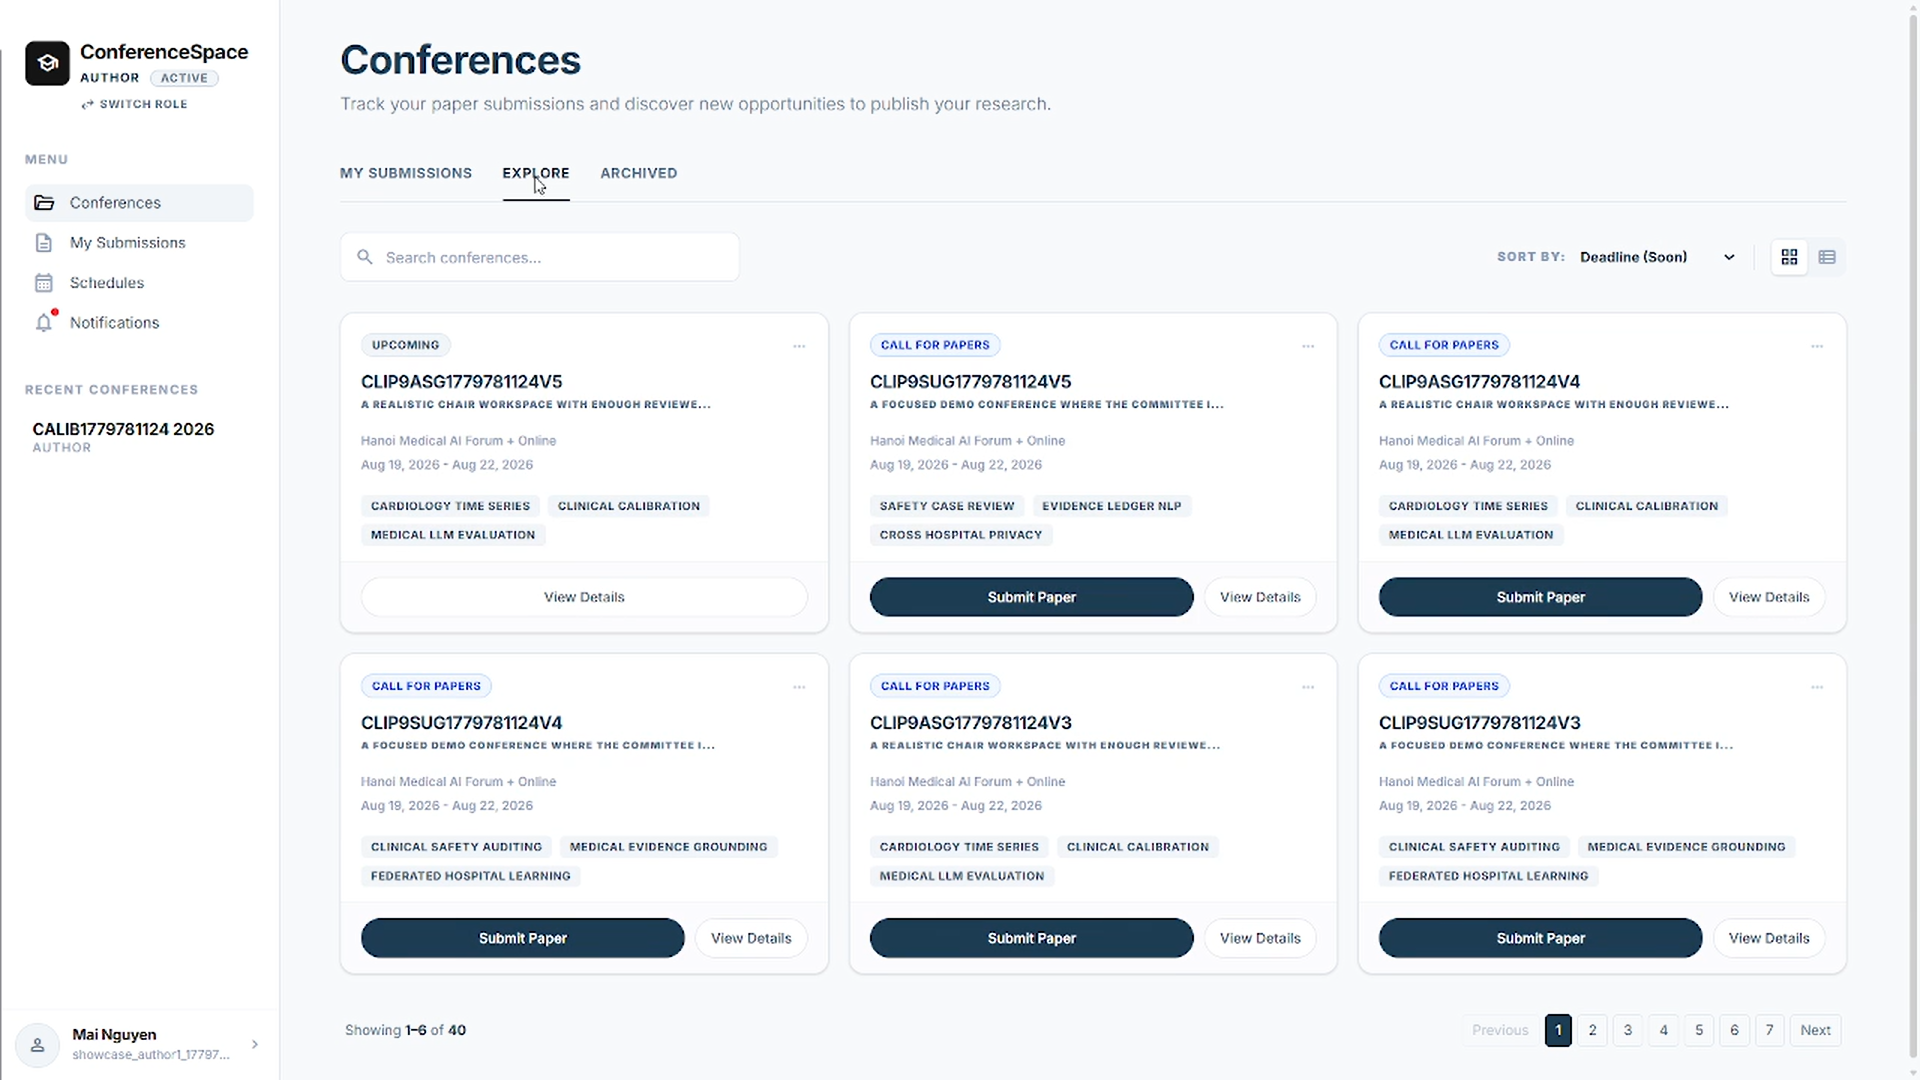
\includegraphics[width=0.95\textwidth]{images/chapter_3_uc01_explore_conferences.png}
  \caption{Giao diện khám phá danh sách hội nghị mặc định}
  \label{fig:uc01-explore-cut}
\end{figure}

Hình~\ref{fig:uc01-explore-cut} minh họa giao diện danh sách hội nghị mặc định mà Tác giả nhìn thấy khi bắt đầu tìm kiếm.

\begin{figure}[H]
  \centering
  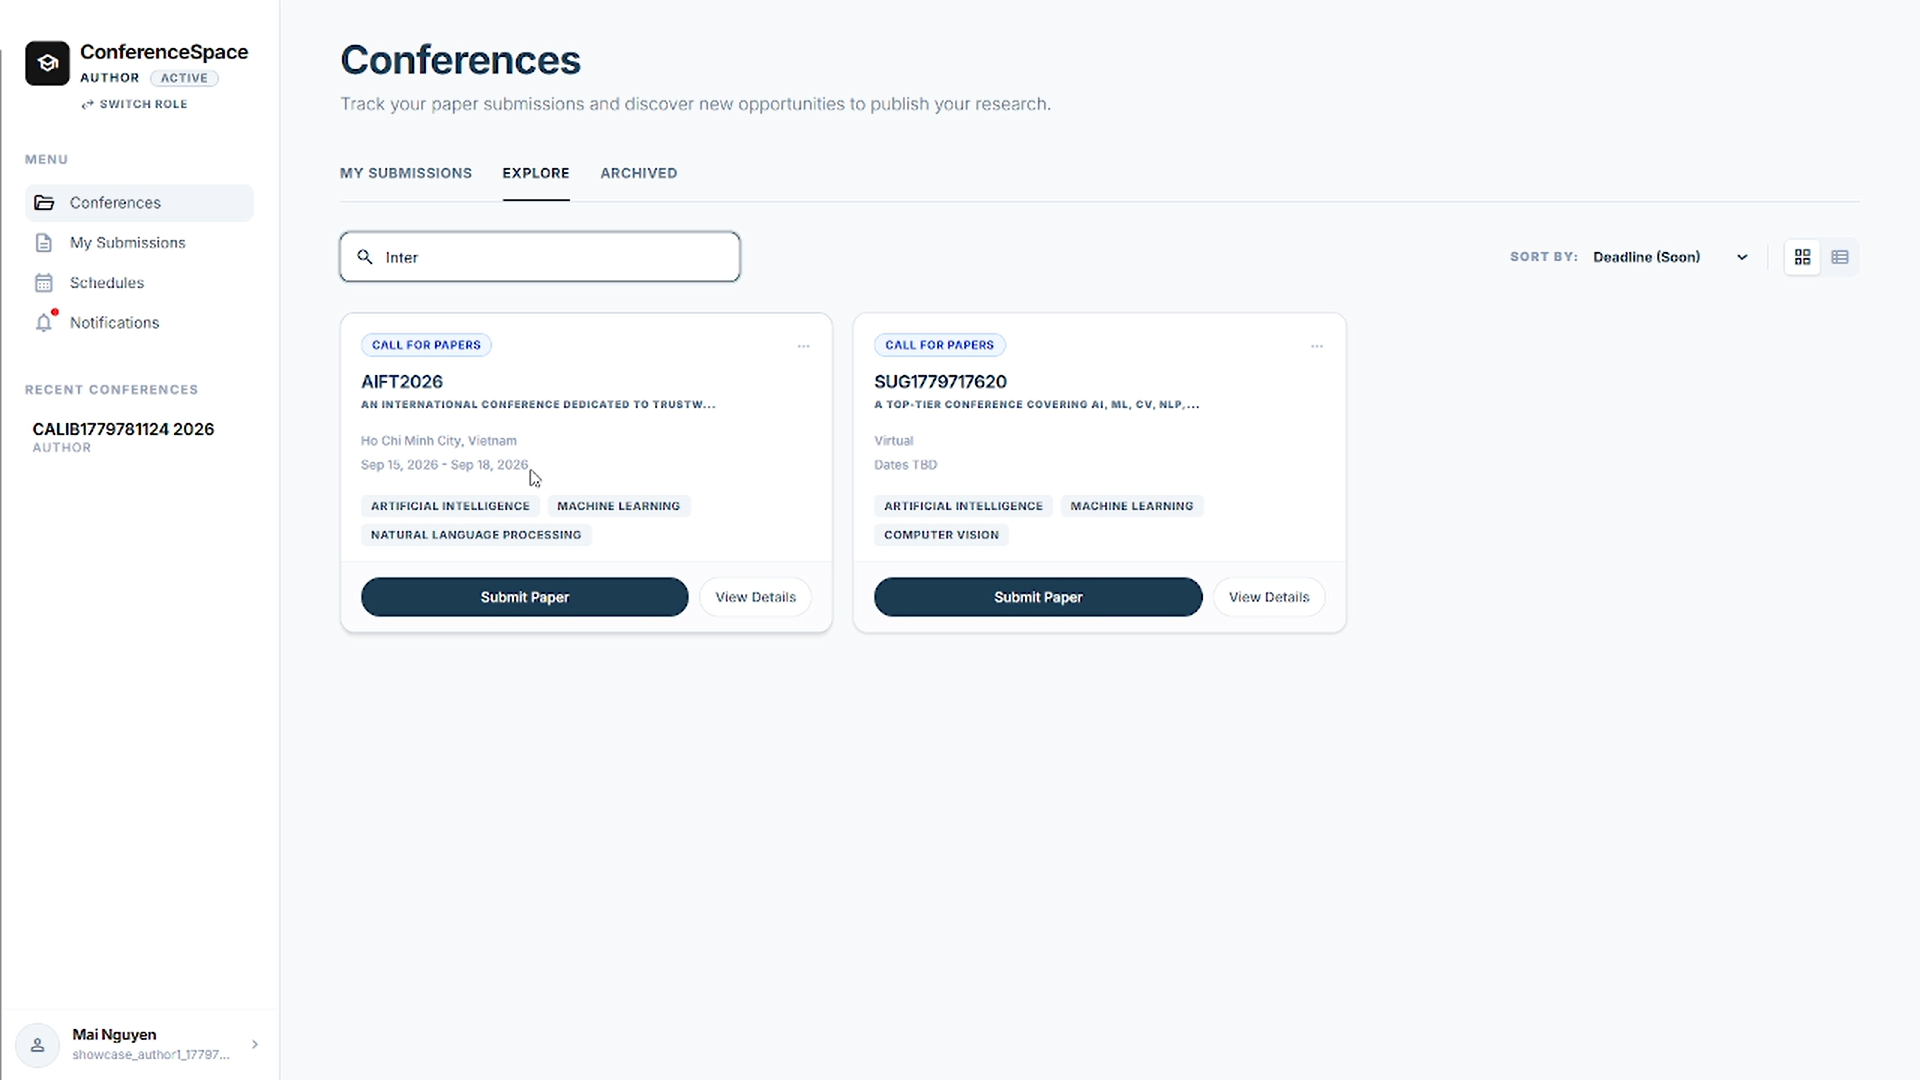
\includegraphics[width=0.95\textwidth]{images/chapter_3_uc01_search_conferences.png}
  \caption{Kết quả tìm kiếm và áp dụng bộ lọc động}
  \label{fig:uc01-search-cut}
\end{figure}

Hình~\ref{fig:uc01-search-cut} minh họa kết quả tìm kiếm sau khi Tác giả áp dụng bộ lọc động.

\begin{figure}[H]
  \centering
  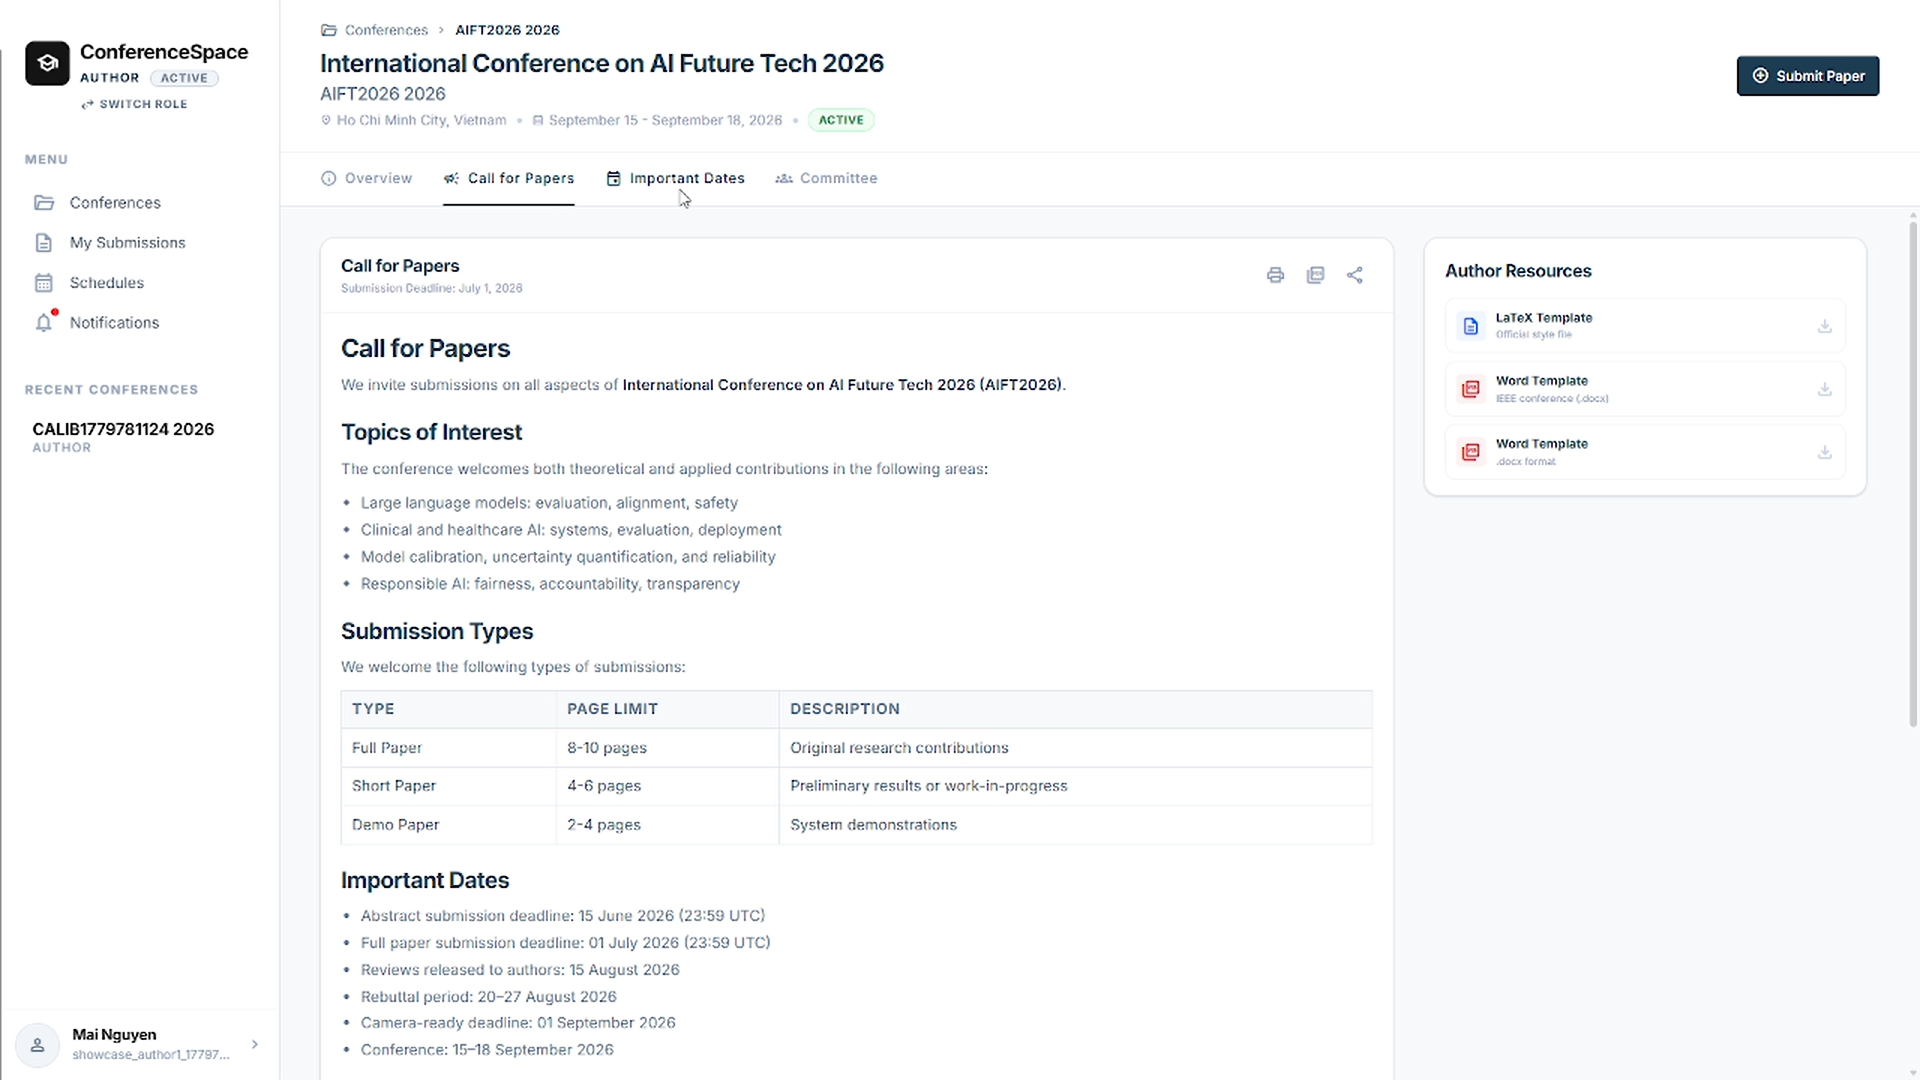
\includegraphics[width=0.95\textwidth]{images/chapter_3_uc01_conference_detail_cfp.png}
  \caption{Giao diện trang chi tiết hội nghị: Tab kêu gọi nộp bài (Call for Papers)}
  \label{fig:uc01-detail-cfp-cut}
\end{figure}

Hình~\ref{fig:uc01-detail-cfp-cut} thể hiện tab kêu gọi nộp bài (Call for Papers) trên trang chi tiết hội nghị.

\begin{figure}[H]
  \centering
  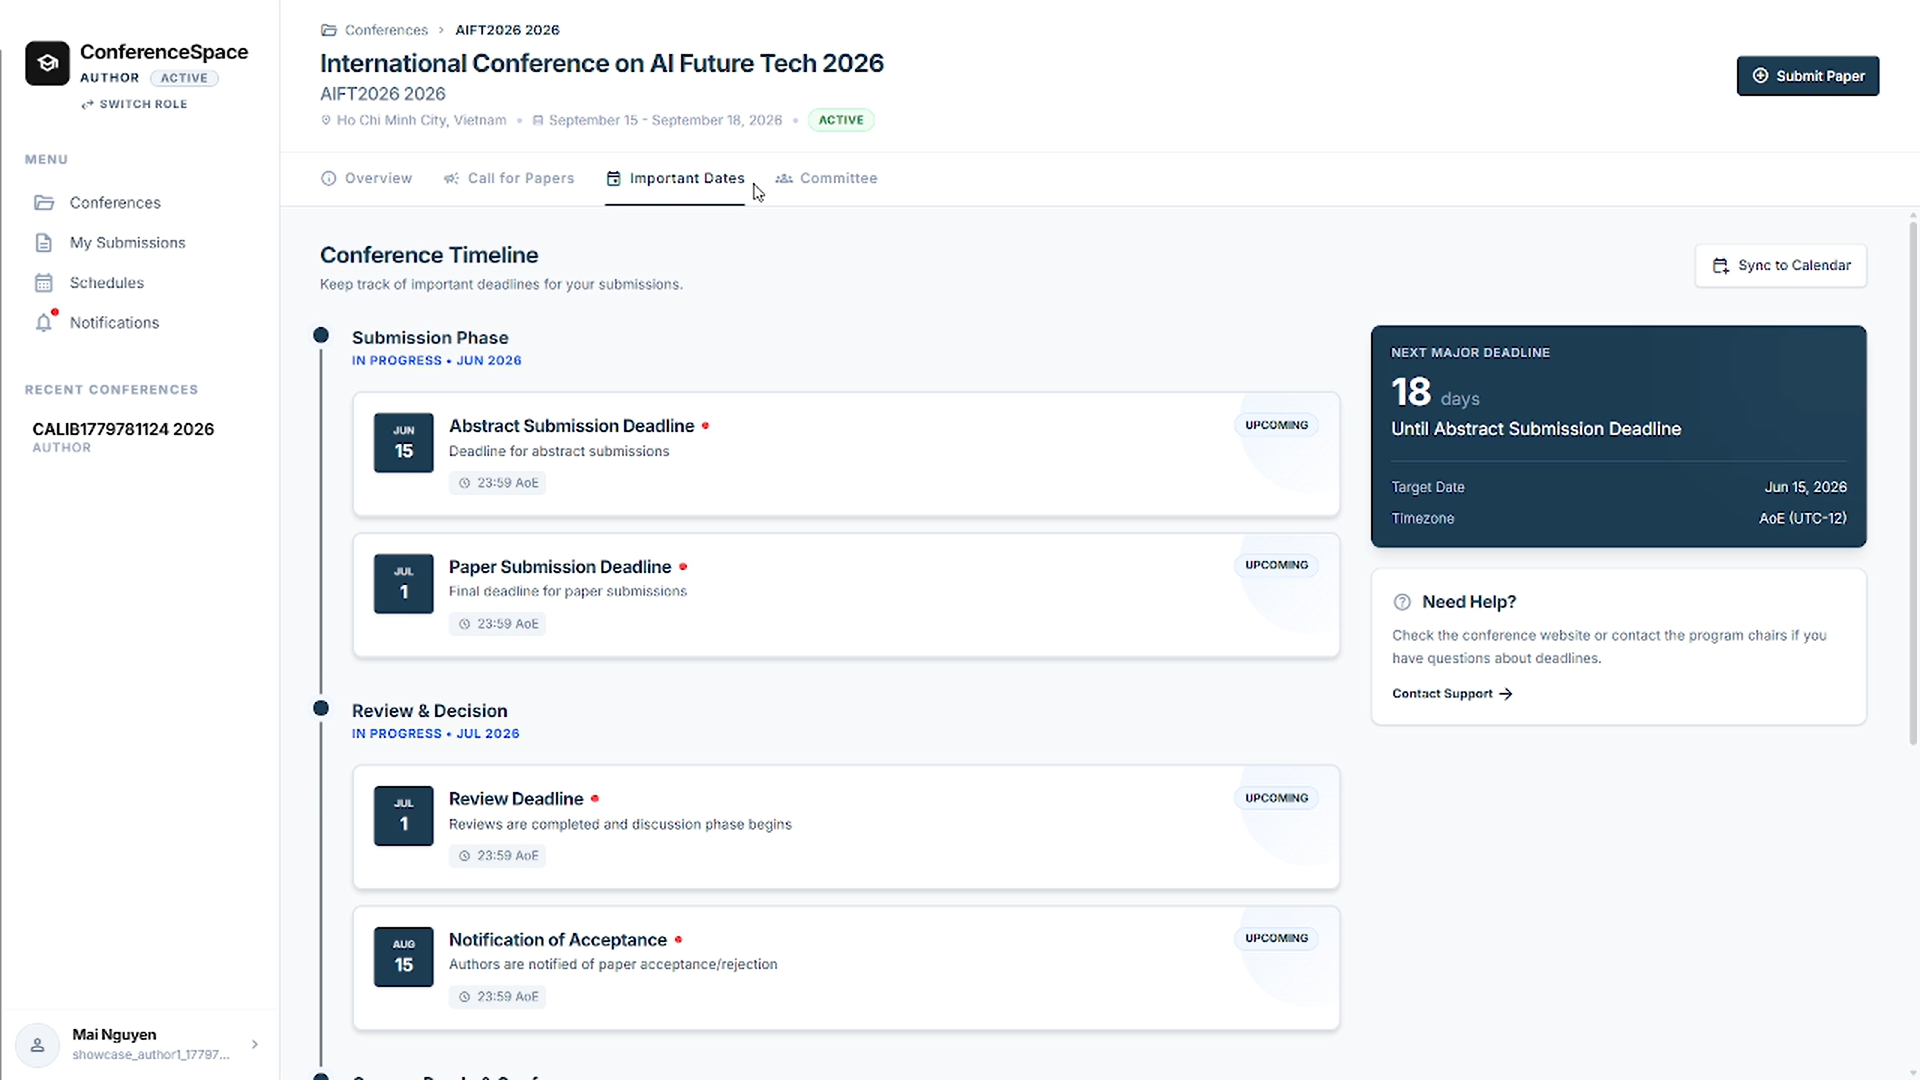
\includegraphics[width=0.95\textwidth]{images/chapter_3_uc01_conference_detail_dates.png}
  \caption{Giao diện trang chi tiết hội nghị: Tab mốc thời gian quan trọng (Important Dates)}
  \label{fig:uc01-detail-dates-cut}
\end{figure}


Hình~\ref{fig:uc01-detail-dates-cut} thể hiện tab mốc thời gian quan trọng trên trang chi tiết hội nghị.

\begin{figure}[H]
  \centering
  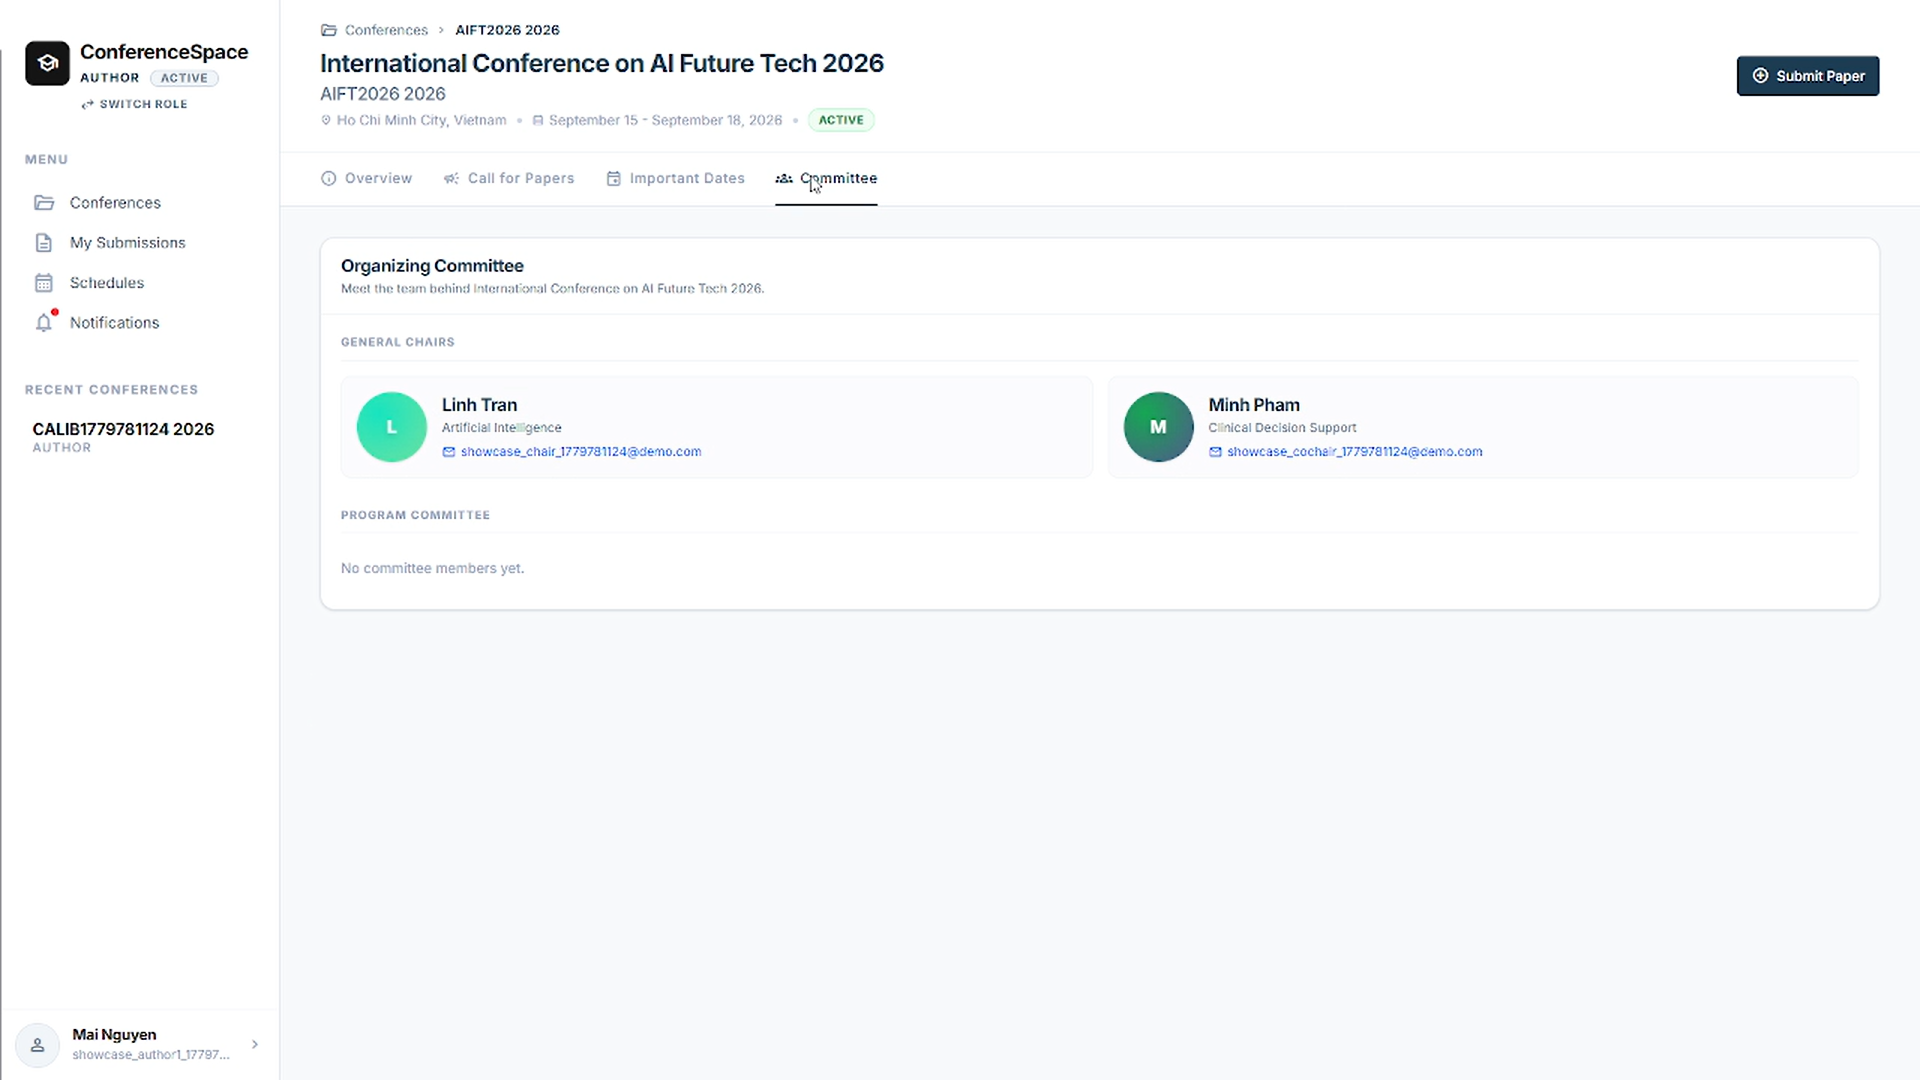
\includegraphics[width=0.95\textwidth]{images/chapter_3_uc01_conference_detail_committee.png}
  \caption{Giao diện trang chi tiết hội nghị: tab hội đồng chương trình (Committee)}
  \label{fig:uc01-detail-committee-cut}
\end{figure}

Hình~\ref{fig:uc01-detail-committee-cut} thể hiện tab hội đồng chương trình trên trang chi tiết hội nghị.

\begin{figure}[H]
  \centering
  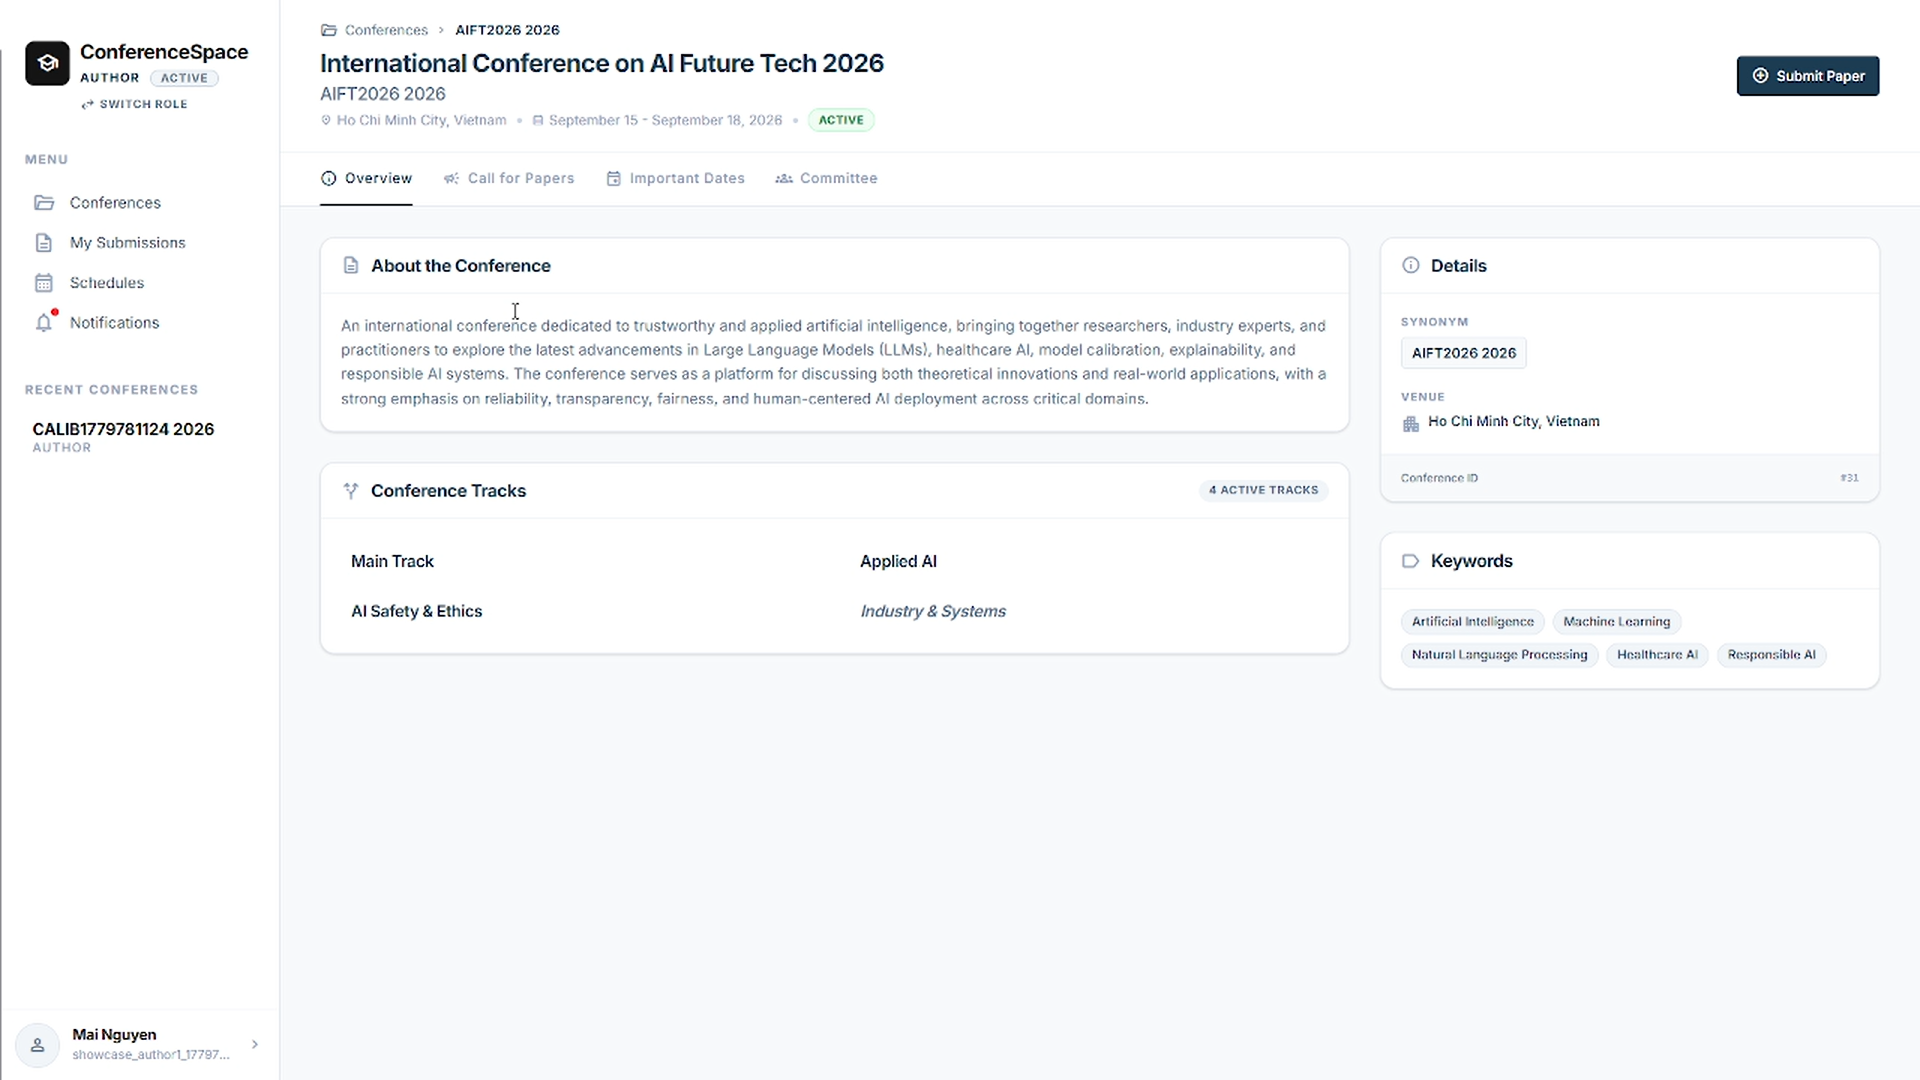
\includegraphics[width=0.95\textwidth]{images/chapter_3_uc01_conference_detail_overview.png}
  \caption{Giao diện trang chi tiết hội nghị: Tab tổng quan (Overview)}
  \label{fig:uc01-detail-overview-cut}
\end{figure}

Hình~\ref{fig:uc01-detail-overview-cut} thể hiện tab tổng quan của trang chi tiết hội nghị mà Tác giả xem trước khi quyết định nộp bài hoặc lưu theo dõi.

\subsubsection{UC-02. Hoàn tất và kiểm tra bài nộp}

Tác giả tạo bản nháp, tải bản thảo và có thể yêu cầu Submission Autofill trích xuất siêu dữ liệu cùng gợi ý chuyên đề trong danh sách hợp lệ. Tác giả kiểm tra, chỉnh sửa thông tin, khai báo đồng tác giả và xung đột lợi ích trước khi Submission Gating kiểm tra tệp, chính sách và các điều kiện gửi bài. Trạng thái \textit{warn} cho phép tiếp tục khi chính sách hội nghị cho phép; trạng thái \textit{block} ngăn gửi cho đến khi lỗi có căn cứ được khắc phục. Nếu Submission Autofill không khả dụng, Tác giả vẫn có thể nhập và lưu bản nháp thủ công. Nếu Submission Gating không trả được bất kỳ kết quả hợp lệ nào, backend chưa cho phép gửi bài cho đến khi thực hiện được một lần kiểm tra hợp lệ.

\begin{figure}[H]
  \centering
  \begin{minipage}{0.48\textwidth}
    \centering
    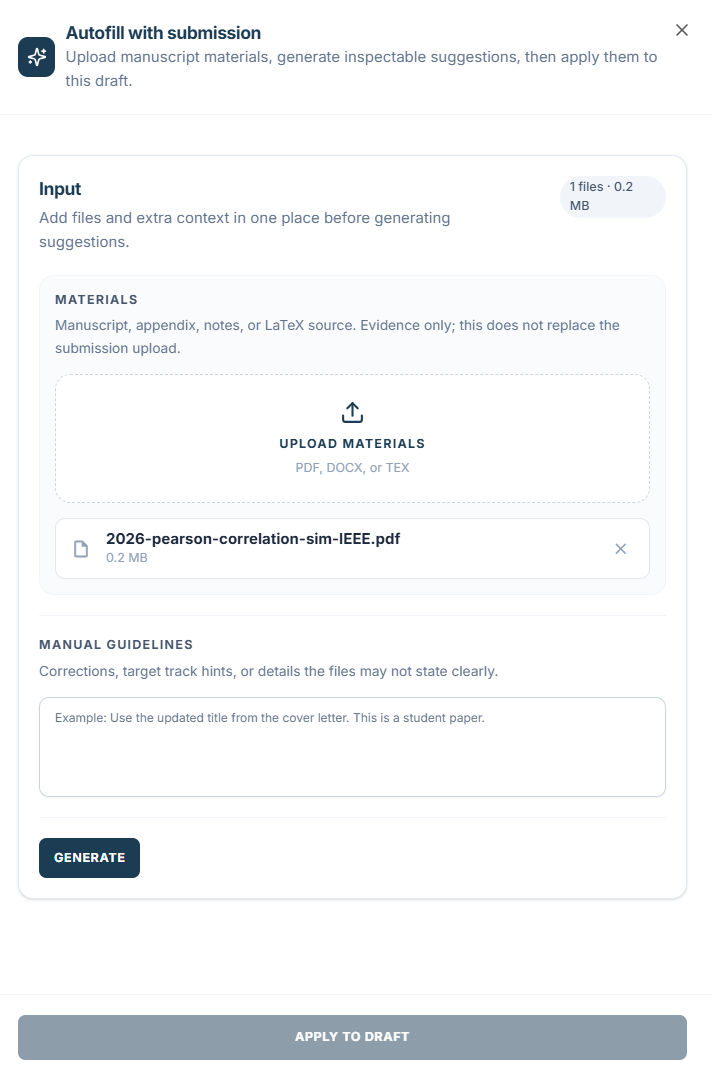
\includegraphics[width=0.56\textwidth]{images/chapter_3_uc02_autofill_1.png}
  \end{minipage}
  \begin{minipage}{0.48\textwidth}
    \centering
    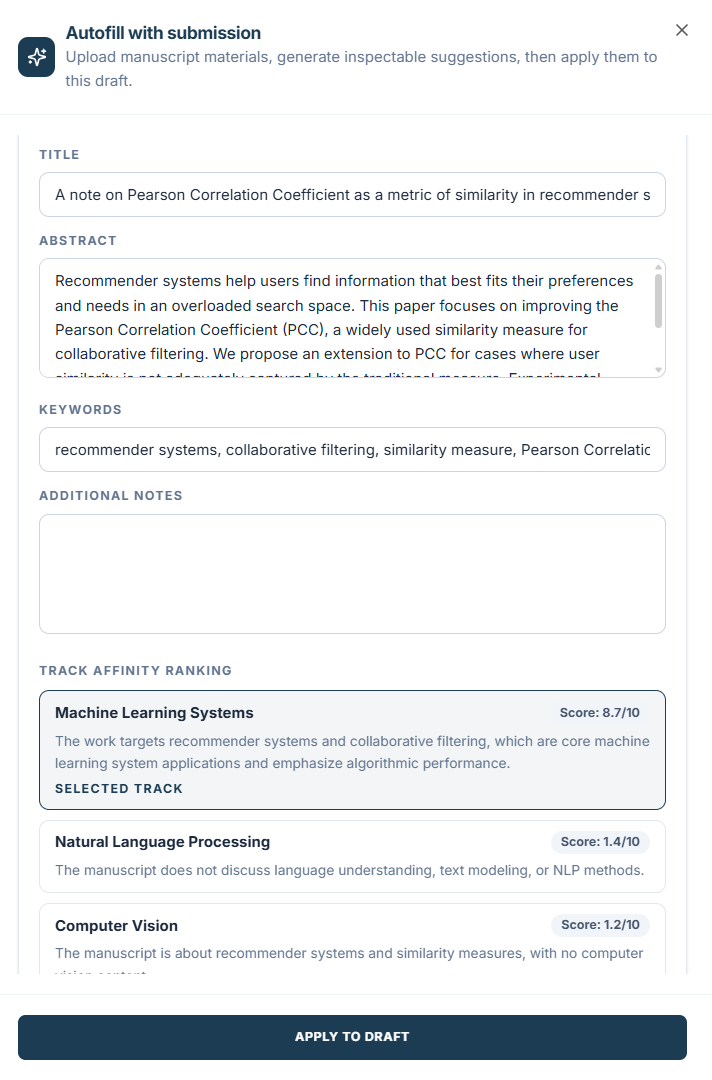
\includegraphics[width=0.56\textwidth]{images/chapter_3_uc02_autofill_2.png}
  \end{minipage}
  \caption{Giao diện tải lên bản thảo (trái) và kết quả trích xuất thông tin tự động (phải)}
  \label{fig:uc02-autofill-cut}
\end{figure}

Hình~\ref{fig:uc02-autofill-cut} trình bày giao diện tải lên bản thảo (trái) cùng kết quả trích xuất thông tin mà Submission Autofill trả về (phải) để Tác giả kiểm tra và chỉnh sửa.

\begin{figure}[H]
  \centering
  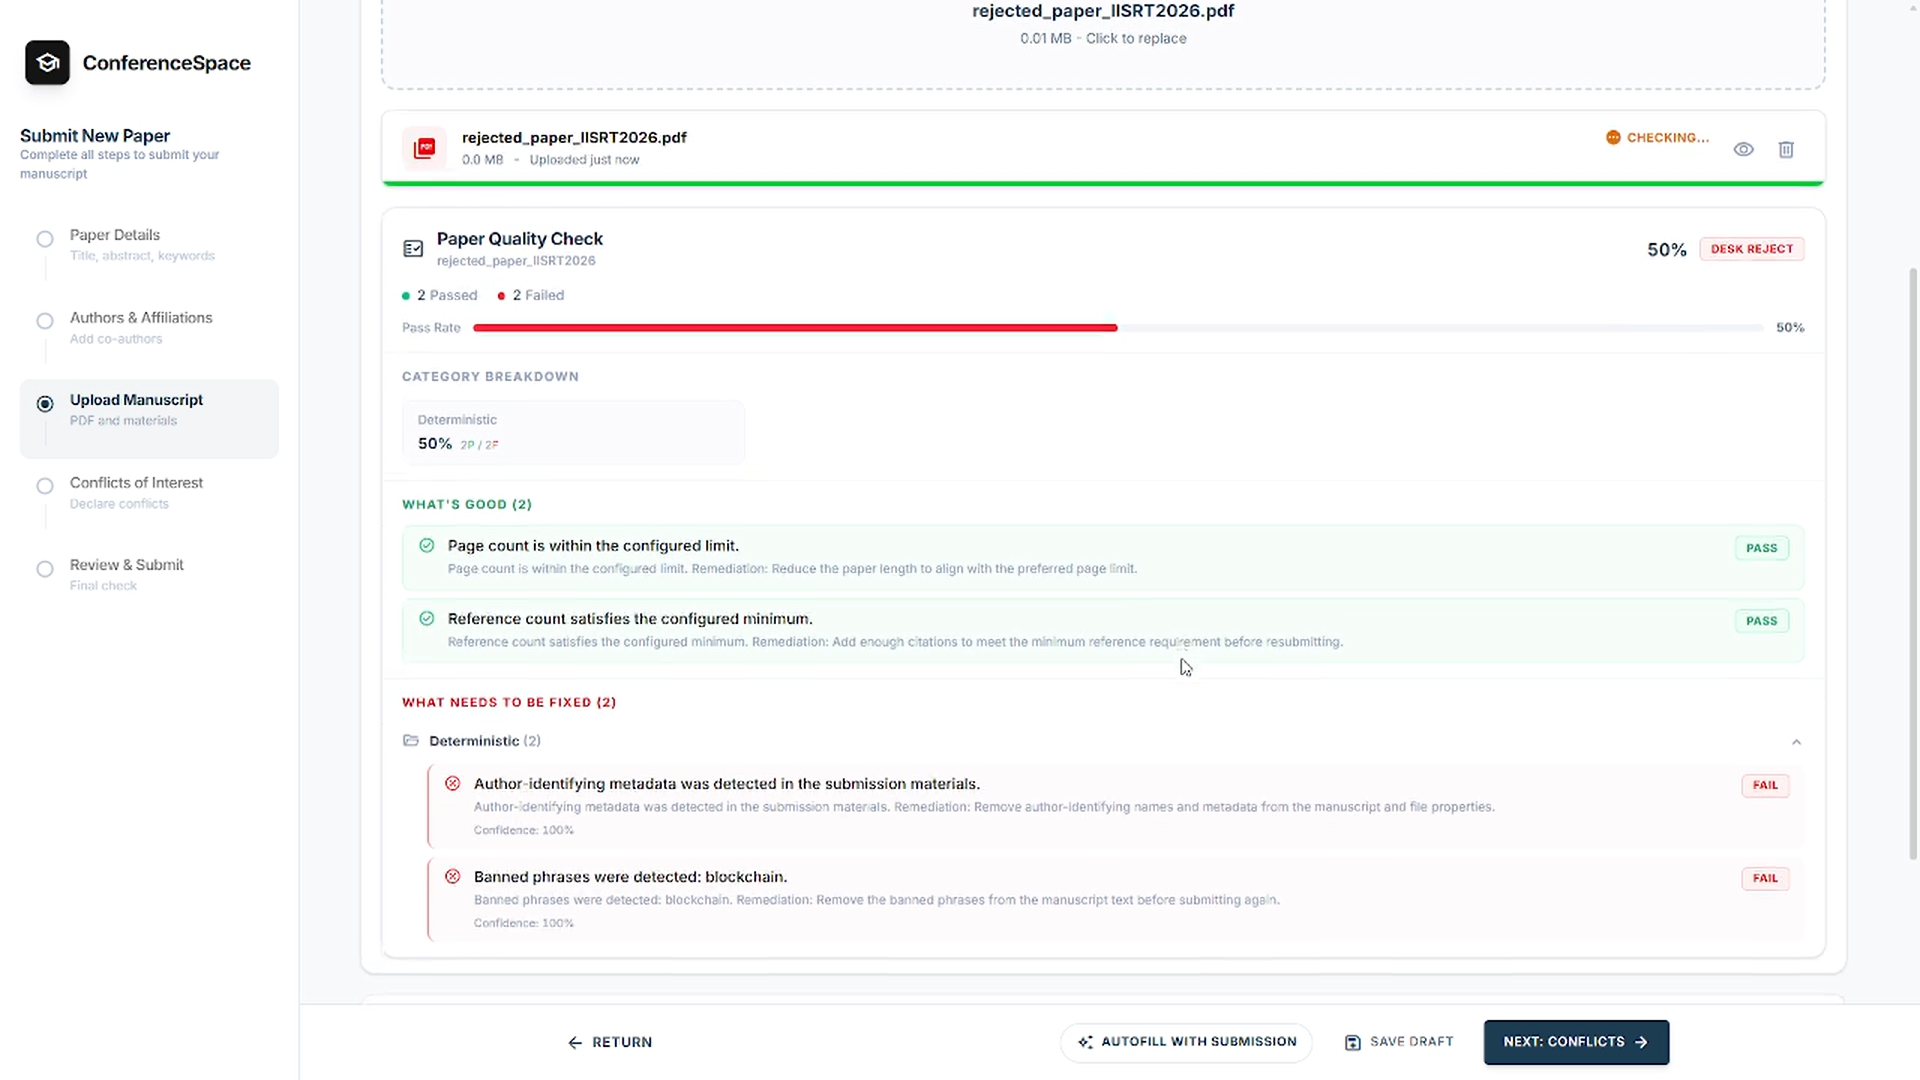
\includegraphics[width=0.95\textwidth]{images/chapter_3_uc02_precheck_gating.png}
  \caption{Kết quả Submission Gating theo ba trạng thái \textit{pass}, \textit{warn} và \textit{block}}
  \label{fig:uc02-gating-cut}
\end{figure}

Trước khi gửi bài, Tác giả xem kết quả kiểm tra tự động của Submission Gating tại Hình~\ref{fig:uc02-gating-cut}, gồm ba trạng thái \textit{pass}, \textit{warn} và \textit{block}.

\begin{figure}[H]
  \centering
  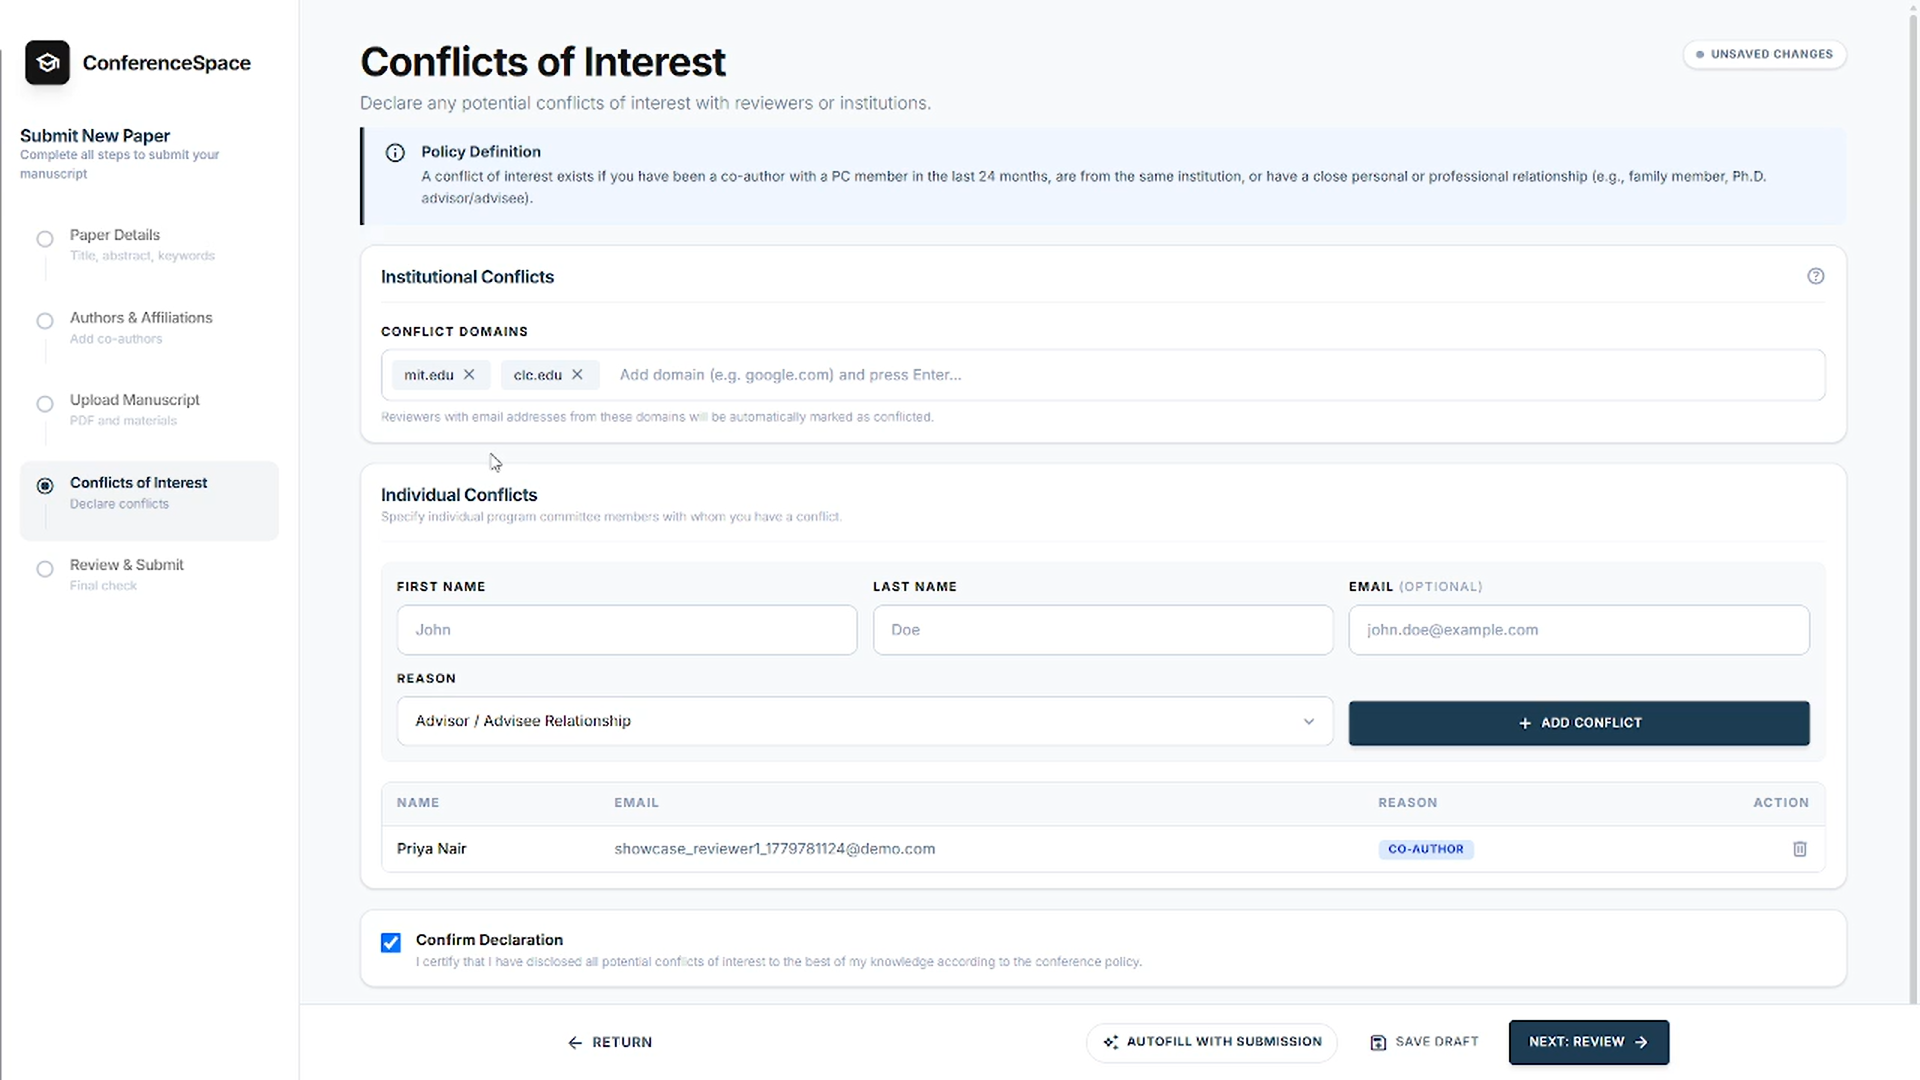
\includegraphics[width=0.95\textwidth]{images/chapter_3_uc02_authors_conflict.png}
  \caption{Giao diện khai báo thông tin các đồng tác giả và xung đột lợi ích}
  \label{fig:uc02-authors-conflict-cut}
\end{figure}

Hình~\ref{fig:uc02-authors-conflict-cut} minh họa giao diện khai báo đồng tác giả và xung đột lợi ích mà Tác giả hoàn tất trước khi Submission Gating kiểm tra.

Hai chức năng AI chỉ hỗ trợ hoàn tất bài nộp: Submission Autofill tạo bản nháp có thể sửa, còn Submission Gating kiểm tra điều kiện trước khi gửi. Tác giả vẫn là người xác nhận dữ liệu và thực hiện thao tác gửi chính thức.

\subsubsection{UC-03. Quản lý vòng đời bài nộp}

Sau khi tạo bài, Tác giả theo dõi và thực hiện các hành động phù hợp với từng trạng thái: chỉnh sửa bản nháp; theo dõi hoặc rút bài đã gửi khi cấu hình và hạn chót nộp bài cho phép; xem phản biện khi được công bố; gửi phản hồi trong giai đoạn do Chủ tọa hoặc Đồng chủ tọa mở; và tải bản thảo hoàn chỉnh khi bài được chấp nhận. Backend từ chối yêu cầu không phù hợp với trạng thái hoặc hạn chót tương ứng. Phiên bản hiện tại hỗ trợ tải và truy xuất bản thảo hoàn chỉnh nhưng chưa có luồng để Chủ tọa phê duyệt, yêu cầu nộp lại hoặc kiểm tra hạn chót nộp bản thảo hoàn chỉnh tại thời điểm thực thi.

\begin{figure}[H]
  \centering
  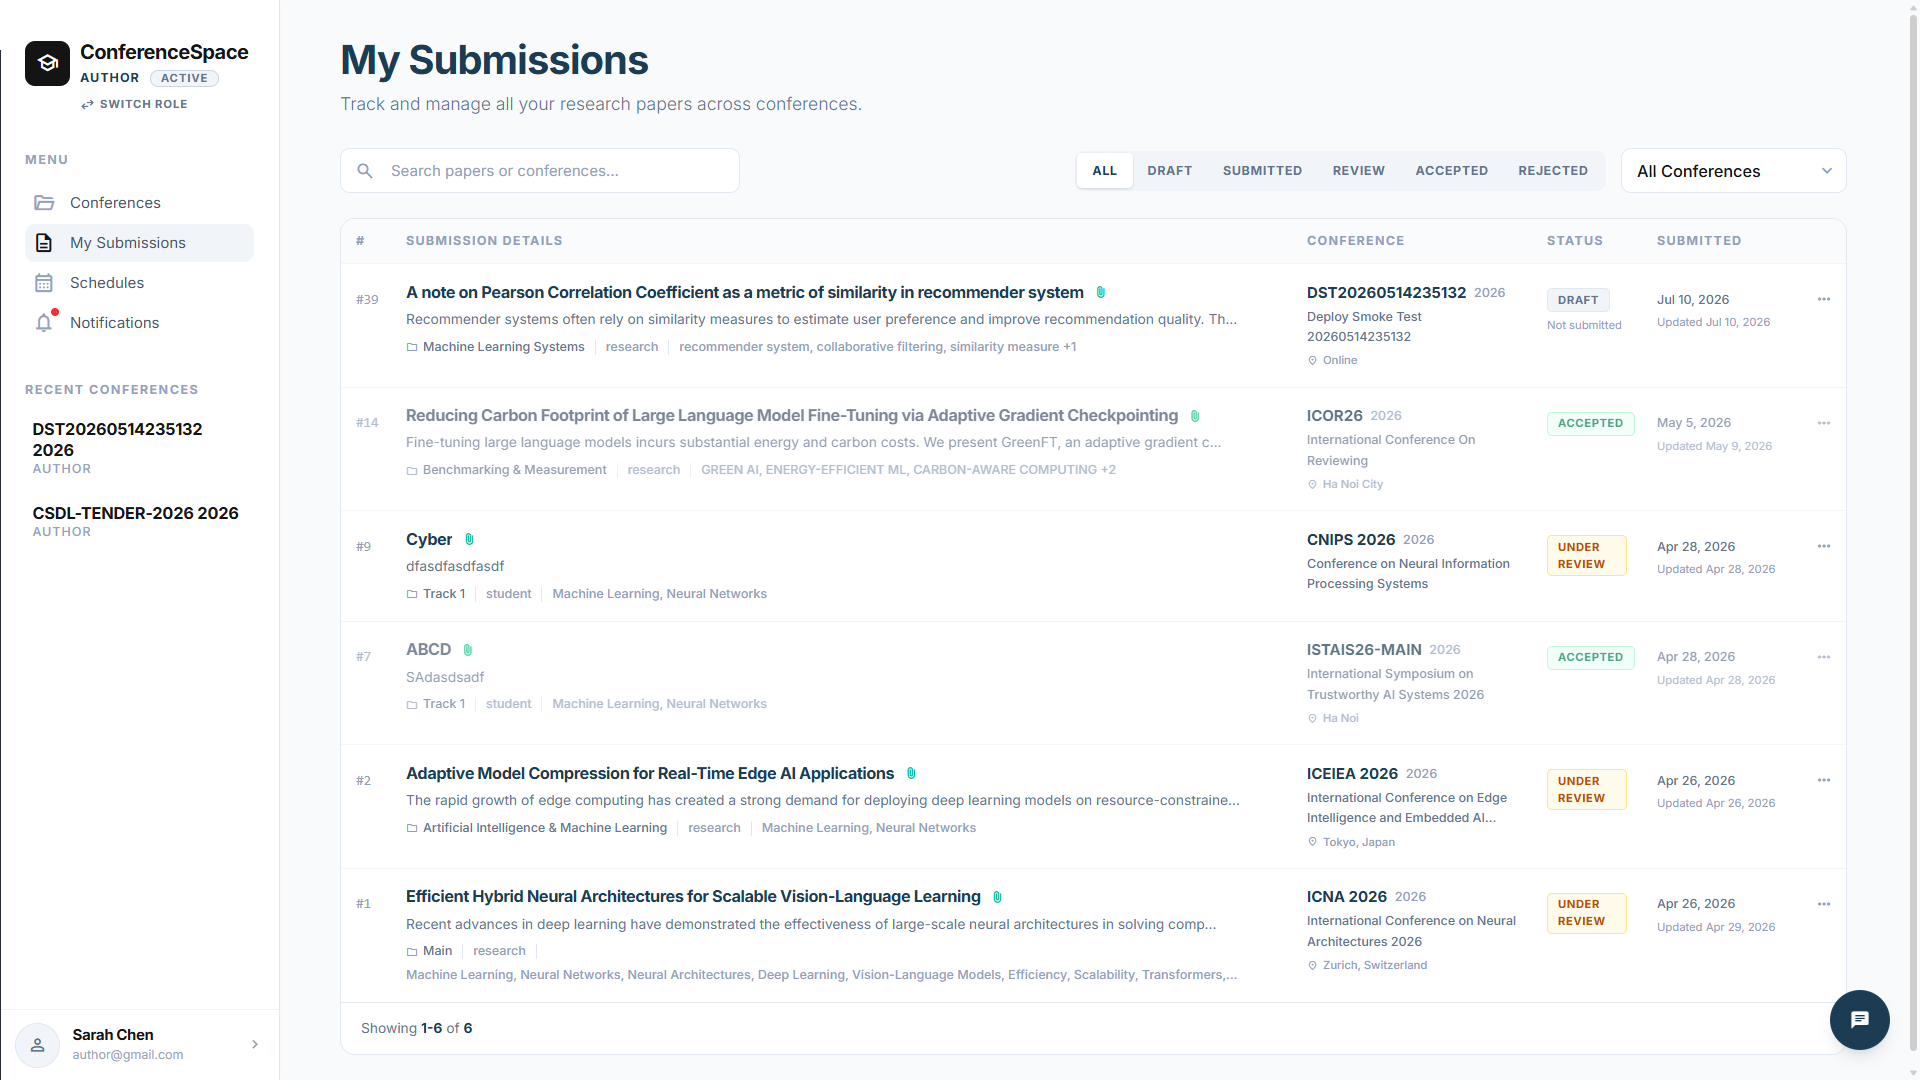
\includegraphics[width=0.95\textwidth]{images/chapter_3_uc03_submissions_list.png}
  \caption{Danh sách bài nộp và trạng thái vòng đời trong không gian làm việc của Tác giả}
  \label{fig:uc03-submissions-cut}
\end{figure}

Giao diện ở Hình~\ref{fig:uc03-submissions-cut} cung cấp một điểm nhìn thống nhất để Tác giả nhận biết trạng thái hiện hành và thao tác nghiệp vụ còn hợp lệ, thay vì chỉ minh họa riêng các chức năng AI ở bước chuẩn bị bài.

\begin{figure}[H]
  \centering
  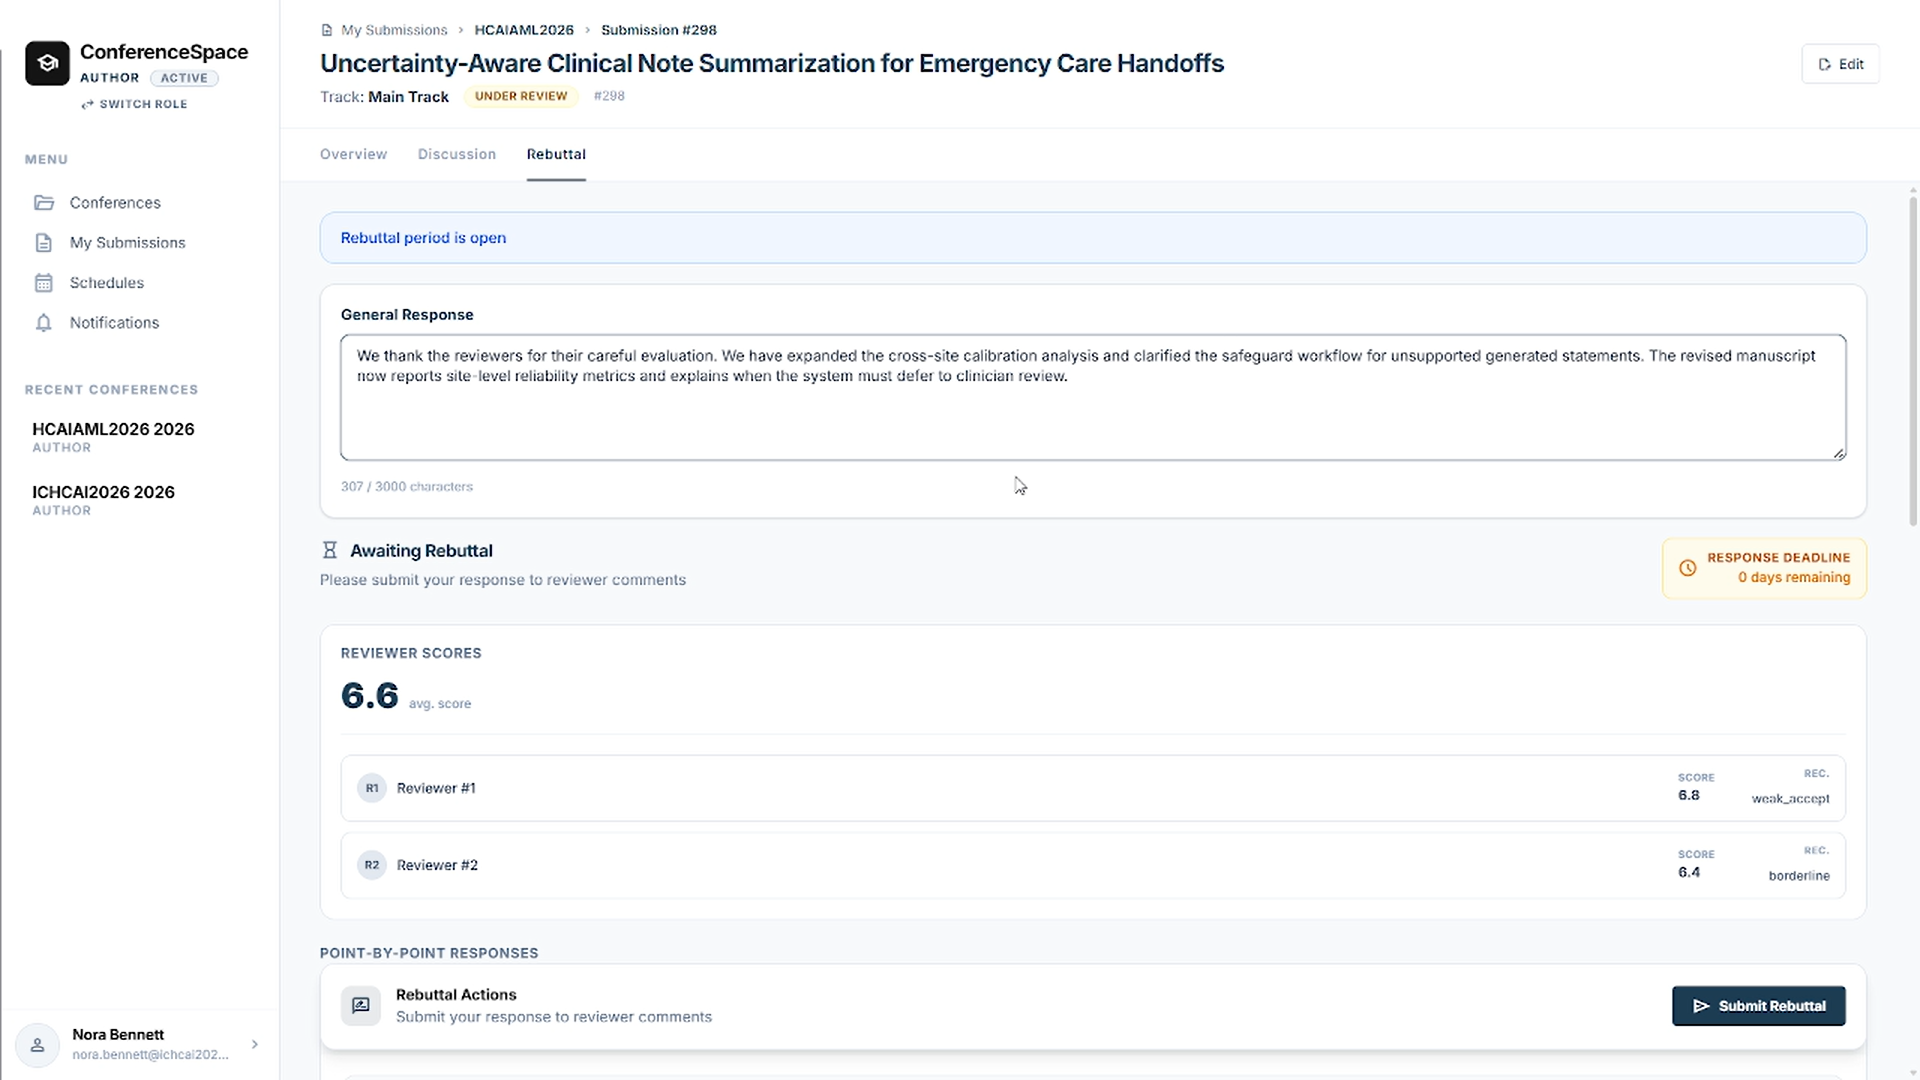
\includegraphics[width=0.95\textwidth]{images/chapter_3_uc03_rebuttal.png}
  \caption{Giao diện soạn thảo và gửi phản hồi của tác giả (rebuttal)}
  \label{fig:uc03-rebuttal-cut}
\end{figure}

Hình~\ref{fig:uc03-rebuttal-cut} minh họa giao diện Tác giả soạn và gửi phản hồi (rebuttal) trong giai đoạn phản hồi.

\begin{figure}[H]
  \centering
  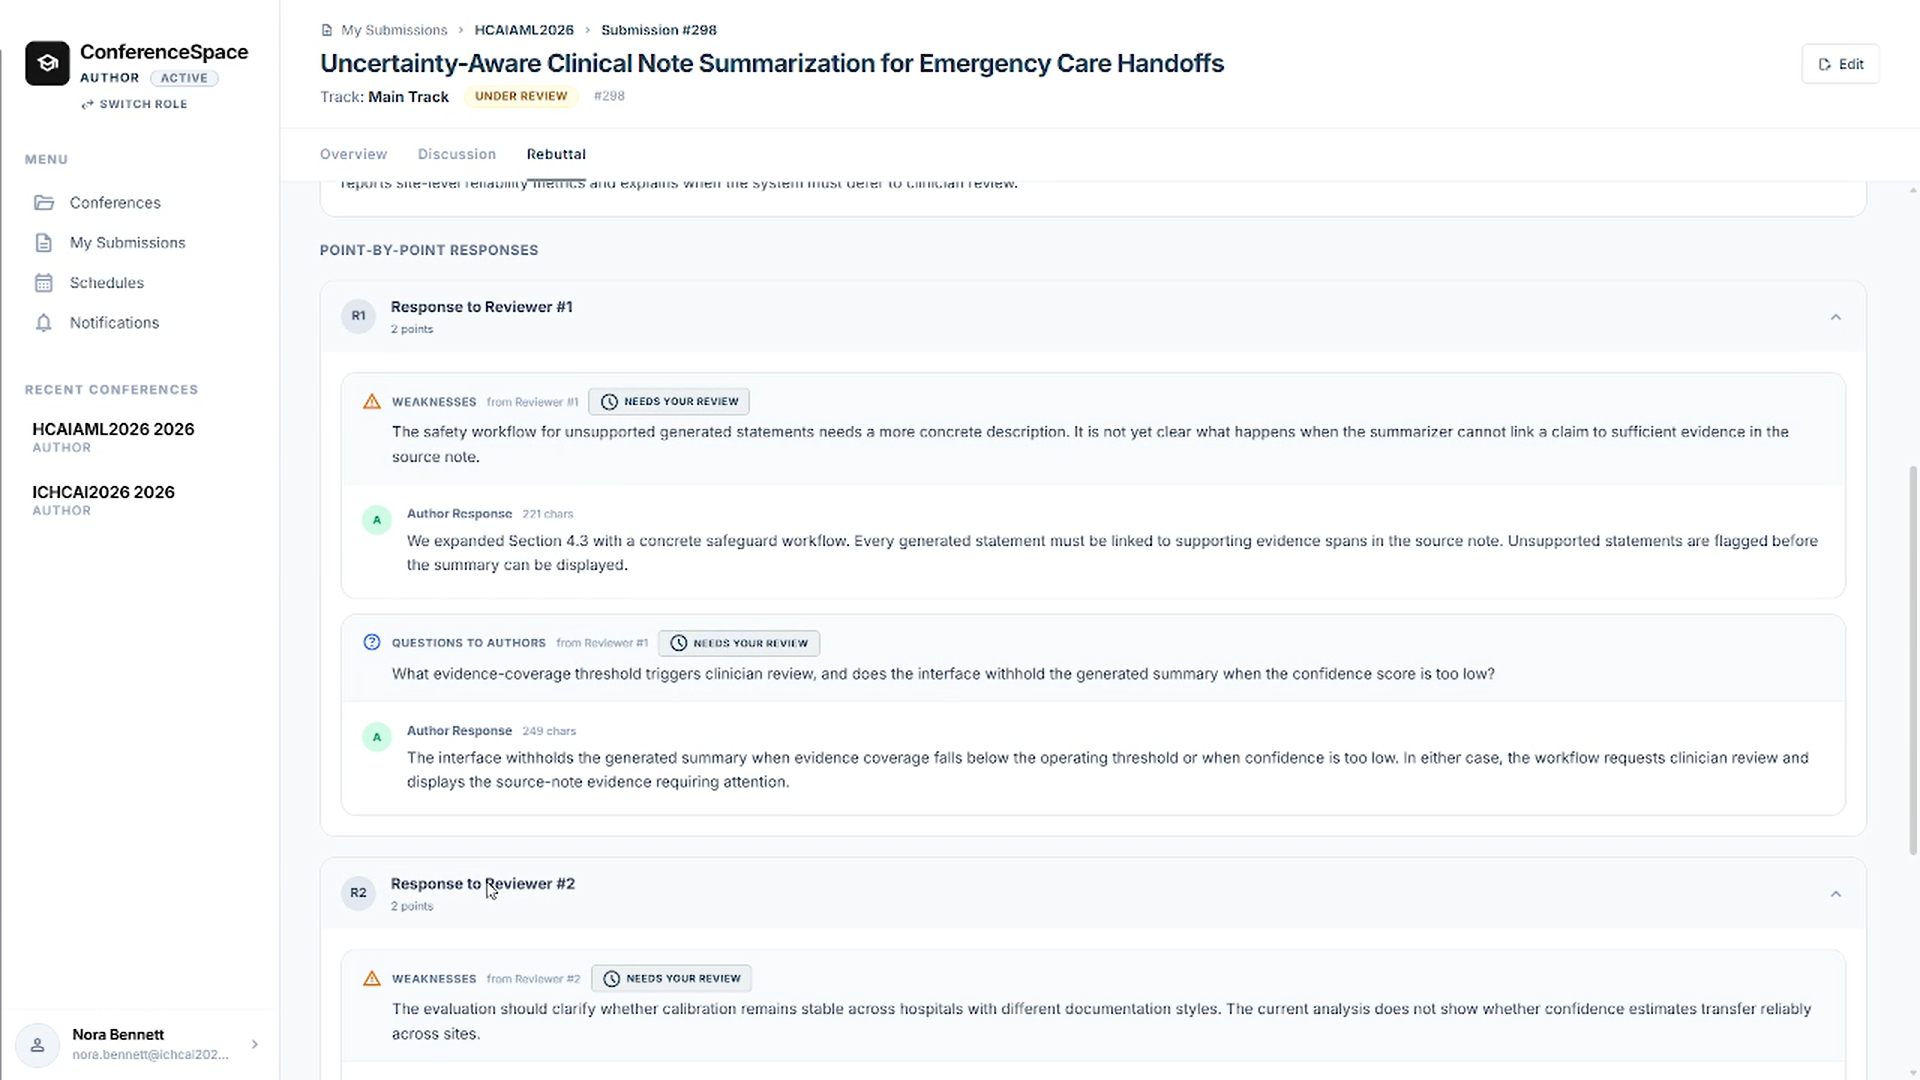
\includegraphics[width=0.95\textwidth]{images/chapter_3_uc03_rebuttal_2.png}
  \caption{Biến thể giao diện soạn và gửi phản hồi của Tác giả (rebuttal)}
  \label{fig:uc03-rebuttal-2-cut}
\end{figure}

Hình~\ref{fig:uc03-rebuttal-2-cut} trình bày một biến thể khác của giao diện soạn thảo và gửi phản hồi.

\begin{figure}[H]
  \centering
  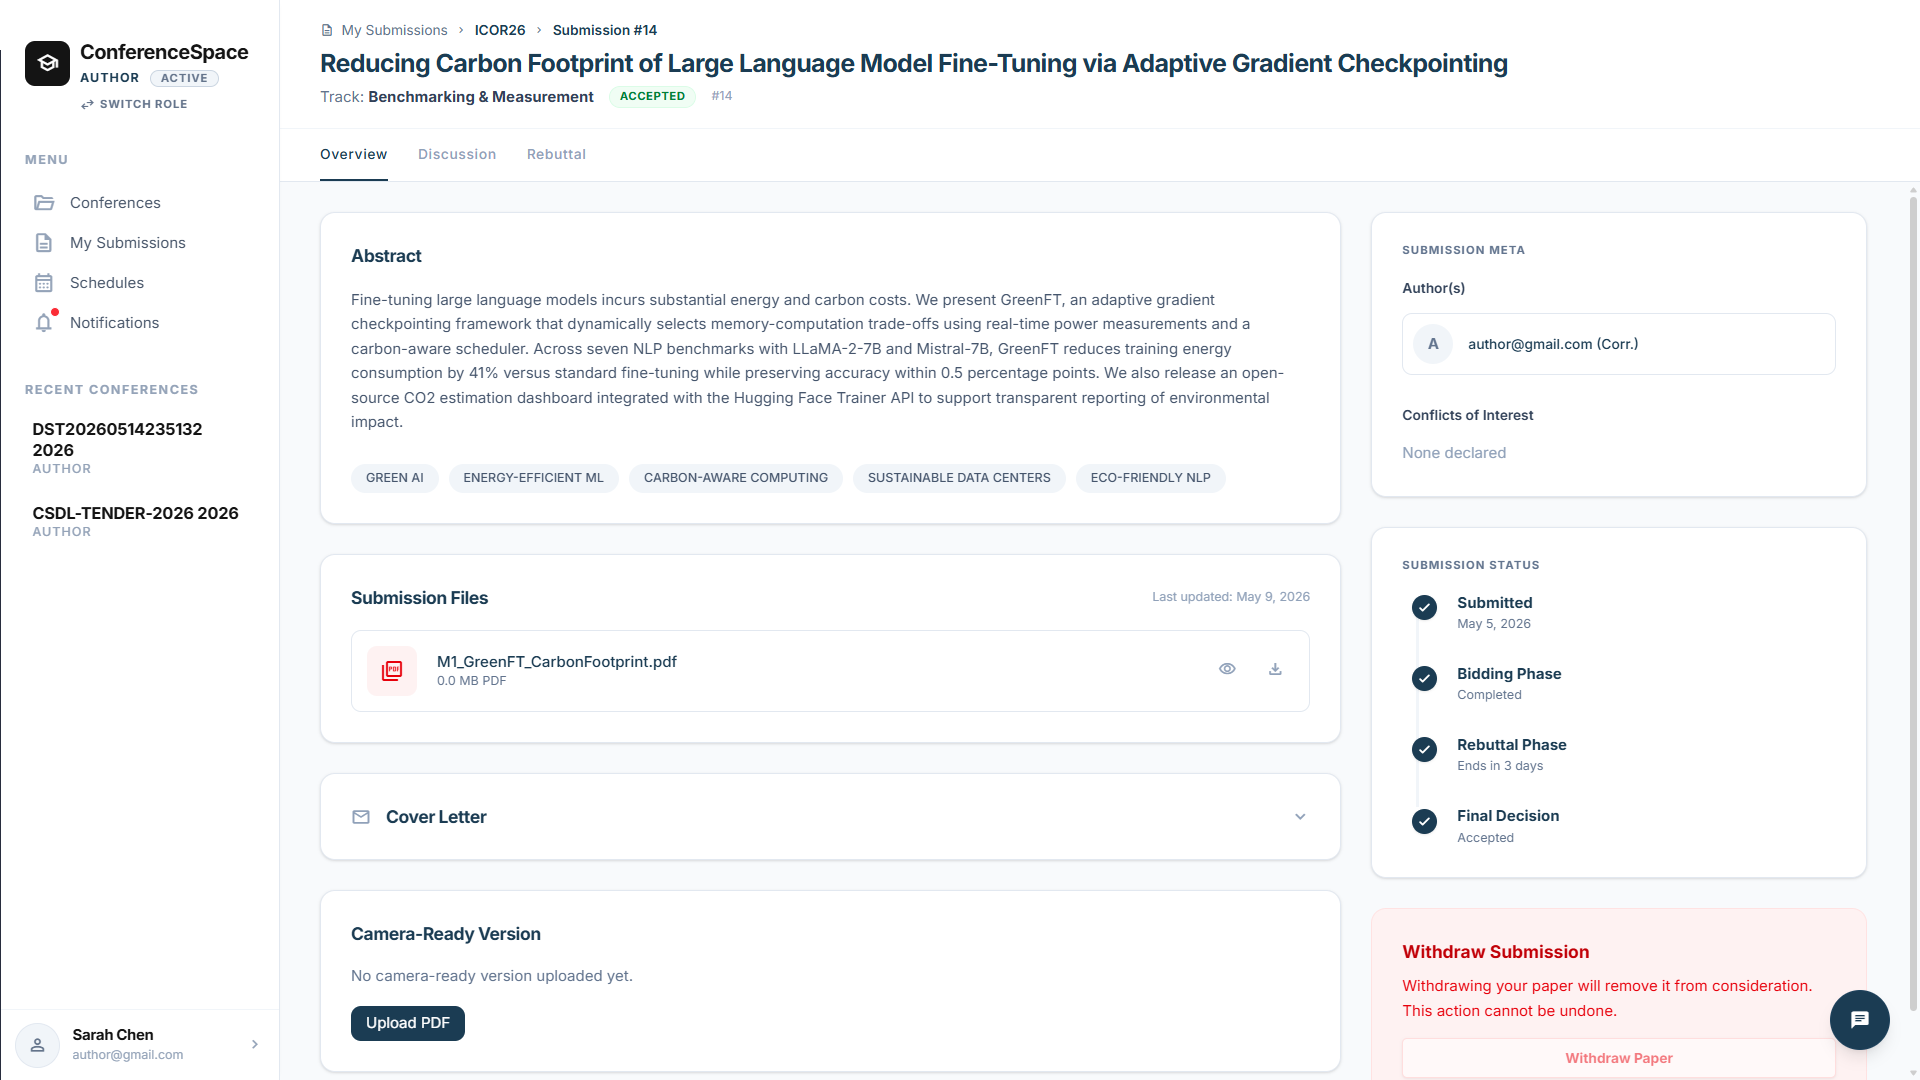
\includegraphics[width=0.95\textwidth]{images/chapter_3_uc03_submission_detail.png}
  \caption{Giao diện trang chi tiết bài nộp, xem nhận định chuyên môn và tải bản thảo hoàn chỉnh (camera-ready)}
  \label{fig:uc03-submission-detail-cut}
\end{figure}

Hình~\ref{fig:uc03-submission-detail-cut} thể hiện trang chi tiết bài nộp, nơi Tác giả xem nhận định chuyên môn và tải lên bản chỉnh sửa cuối cùng khi bài được chấp nhận.

\subsubsection{UC-04. Tiếp nhận lời mời hội nghị và xem bài được phân công}

Chủ tọa gửi lời mời tham gia hội nghị; hệ thống lưu trạng thái và thông báo cho người nhận. Phản biện viên chỉ có thể chấp nhận hoặc từ chối lời mời của chính mình. Đây là trạng thái tham gia hội nghị của Phản biện viên, khác với trạng thái của từng phân công bài. Khi Chủ tọa đã tạo phân công, Phản biện viên xem bài, hạn chót nộp bài và trạng thái trên bảng điều khiển; backend chỉ trả các phân công thuộc người dùng hiện tại. Kho mã nguồn có thao tác phản hồi phân công theo định danh, nhưng luồng giao diện được mô tả trong chương này không đồng nhất thao tác đó với việc chấp nhận lời mời hội nghị.

\begin{figure}[H]
  \centering
  \begin{tabular}{c}
    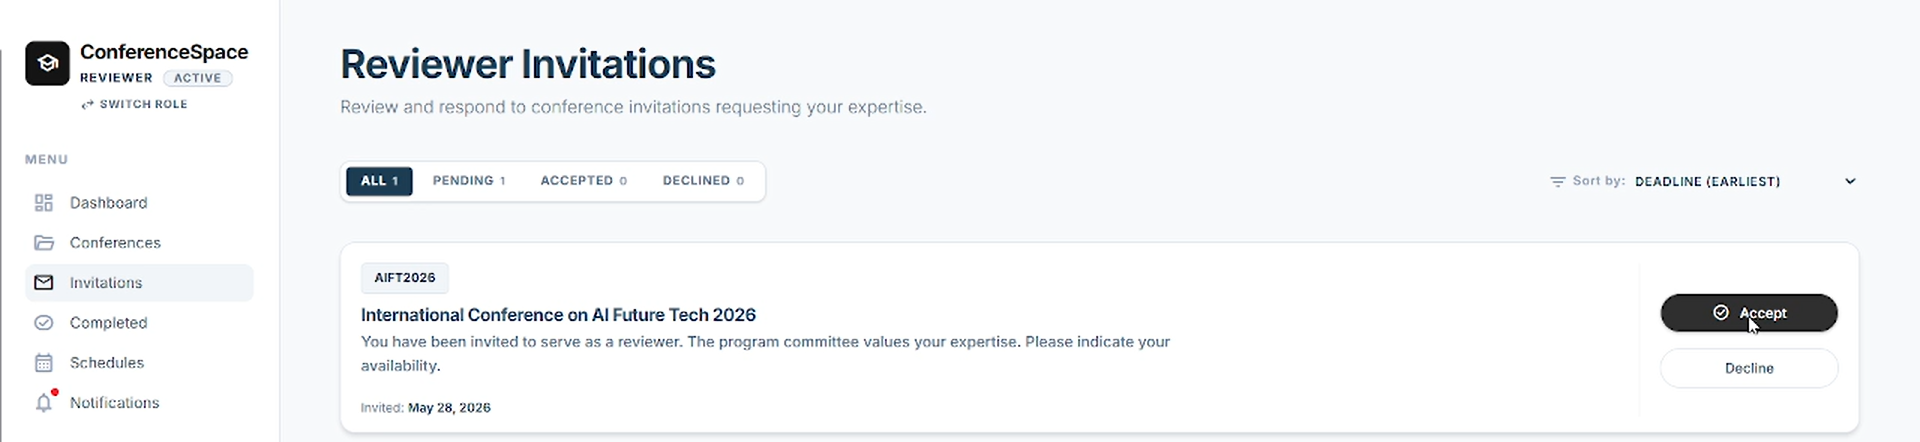
\includegraphics[width=0.95\textwidth]{images/chapter_3_uc04_reviewer_invitations_1.png} \\
    \vspace{0.2cm}
    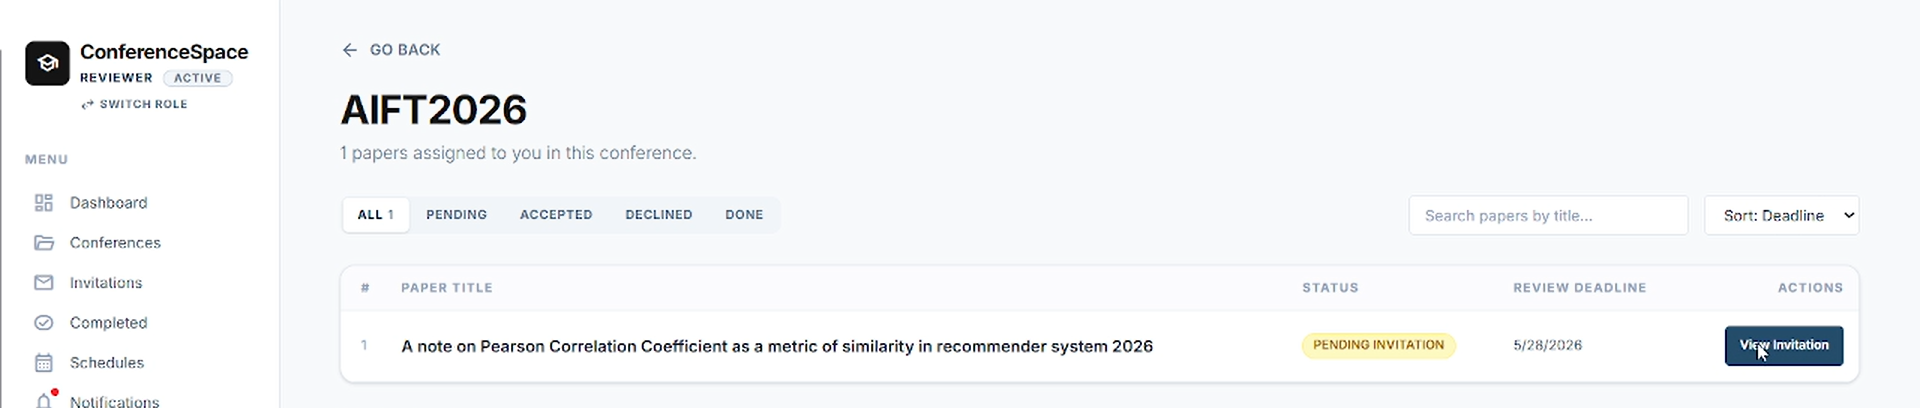
\includegraphics[width=0.95\textwidth]{images/chapter_3_uc04_reviewer_invitations_2.png}
  \end{tabular}
  \caption{Email thông báo lời mời (trên) và danh sách lời mời tham gia phản biện trong hệ thống (dưới)}
  \label{fig:uc04-invitations-cut}
\end{figure}

Hình~\ref{fig:uc04-invitations-cut} minh họa giao diện tiếp nhận thông báo và danh sách lời mời tham gia phản biện hội nghị.

\begin{figure}[H]
  \centering
  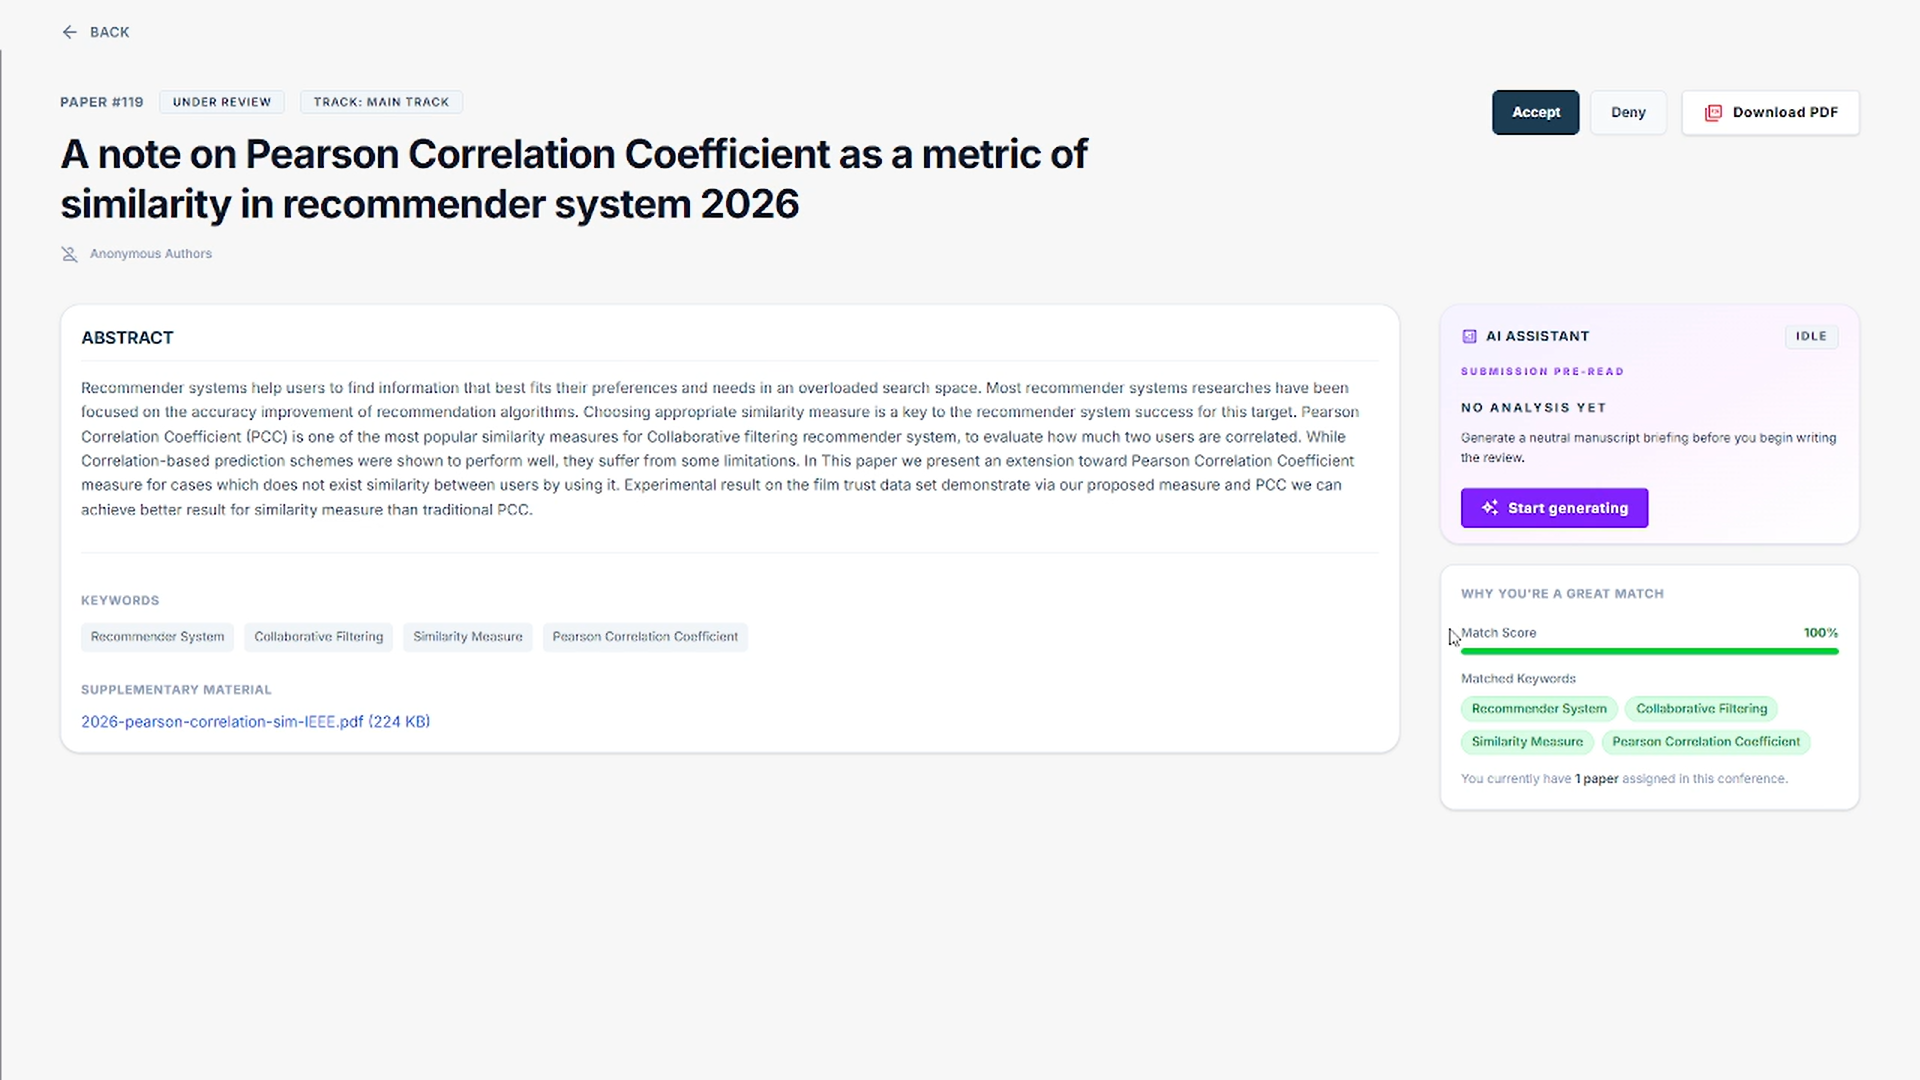
\includegraphics[width=0.95\textwidth]{images/chapter_3_uc04_accept_deny_assignment.png}
  \caption{Giao diện chi tiết bài nộp để Phản biện viên chấp nhận hoặc từ chối phân công}
  \label{fig:uc04-accept-deny-cut}
\end{figure}

Sau khi Chủ tọa tạo phân công, Phản biện viên dùng giao diện tại Hình~\ref{fig:uc04-accept-deny-cut} để xem bài nộp và chấp nhận hoặc từ chối phân công.

\subsubsection{UC-05. Đọc, soạn và gửi phản biện có AI hỗ trợ}

Phản biện viên mở bài được phân công, đọc bản thảo và nhập điểm, nhận xét, khuyến nghị cùng mức độ tự tin. Reviewer Initial Analysis có thể cung cấp bản định hướng ban đầu, nhưng Phản biện viên phải đối chiếu nội dung này với bài gốc và tự hình thành nhận định. Trước khi gửi, Review Quality Auditor rà soát mức độ đầy đủ, cụ thể và nhất quán của bản nháp. Phản biện viên xem các phát hiện, chỉnh sửa khi cần và xác nhận gửi phản biện.

\begin{figure}[H]
  \centering
  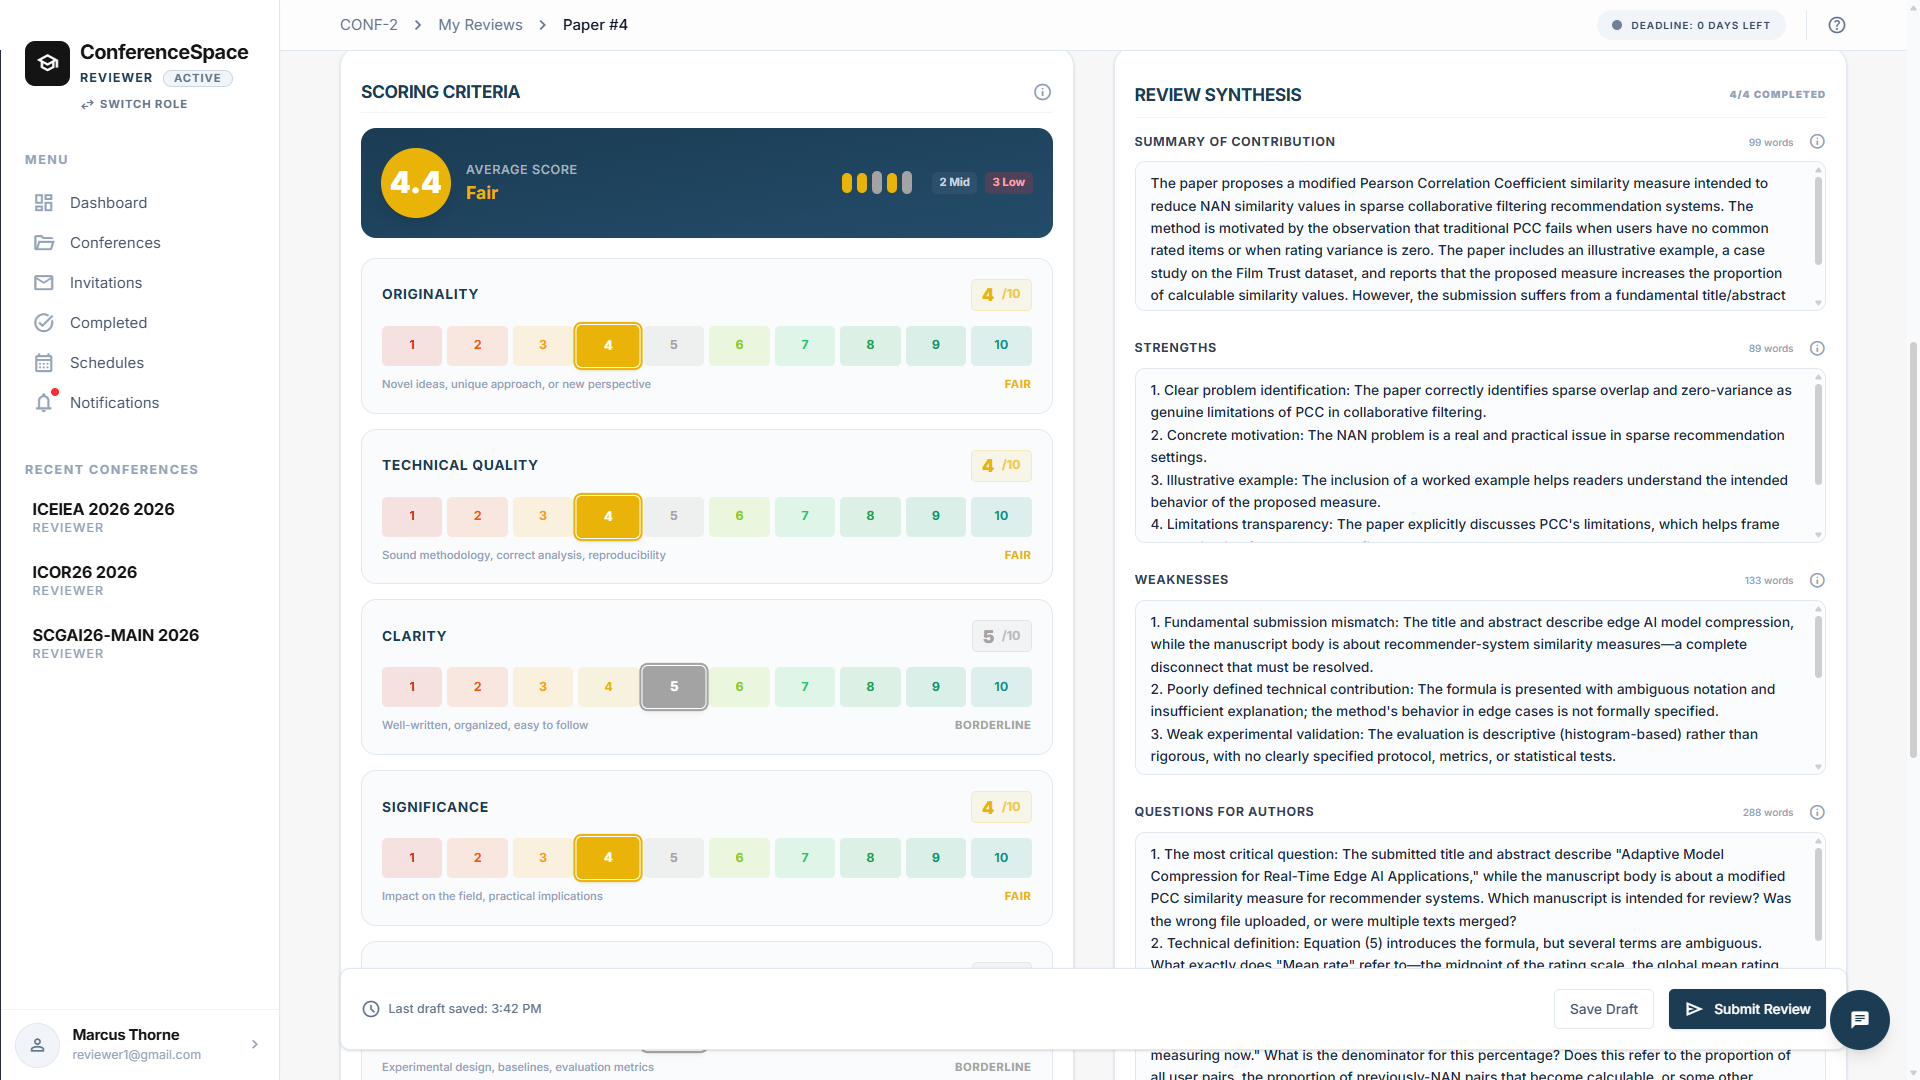
\includegraphics[width=0.95\textwidth]{images/chapter_3_uc05_reviewer_workspace_1.png}
  \caption{Không gian đọc bài và soạn phản biện của Phản biện viên}
  \label{fig:uc05-workspace-cut}
\end{figure}

Hình~\ref{fig:uc05-workspace-cut} đặt hai chức năng AI vào đúng bối cảnh sử dụng: chúng hỗ trợ một quy trình mà Phản biện viên vẫn phải đọc bản thảo, nhập nhận xét và chịu trách nhiệm về bản phản biện cuối cùng.

\begin{figure}[H]
  \centering
  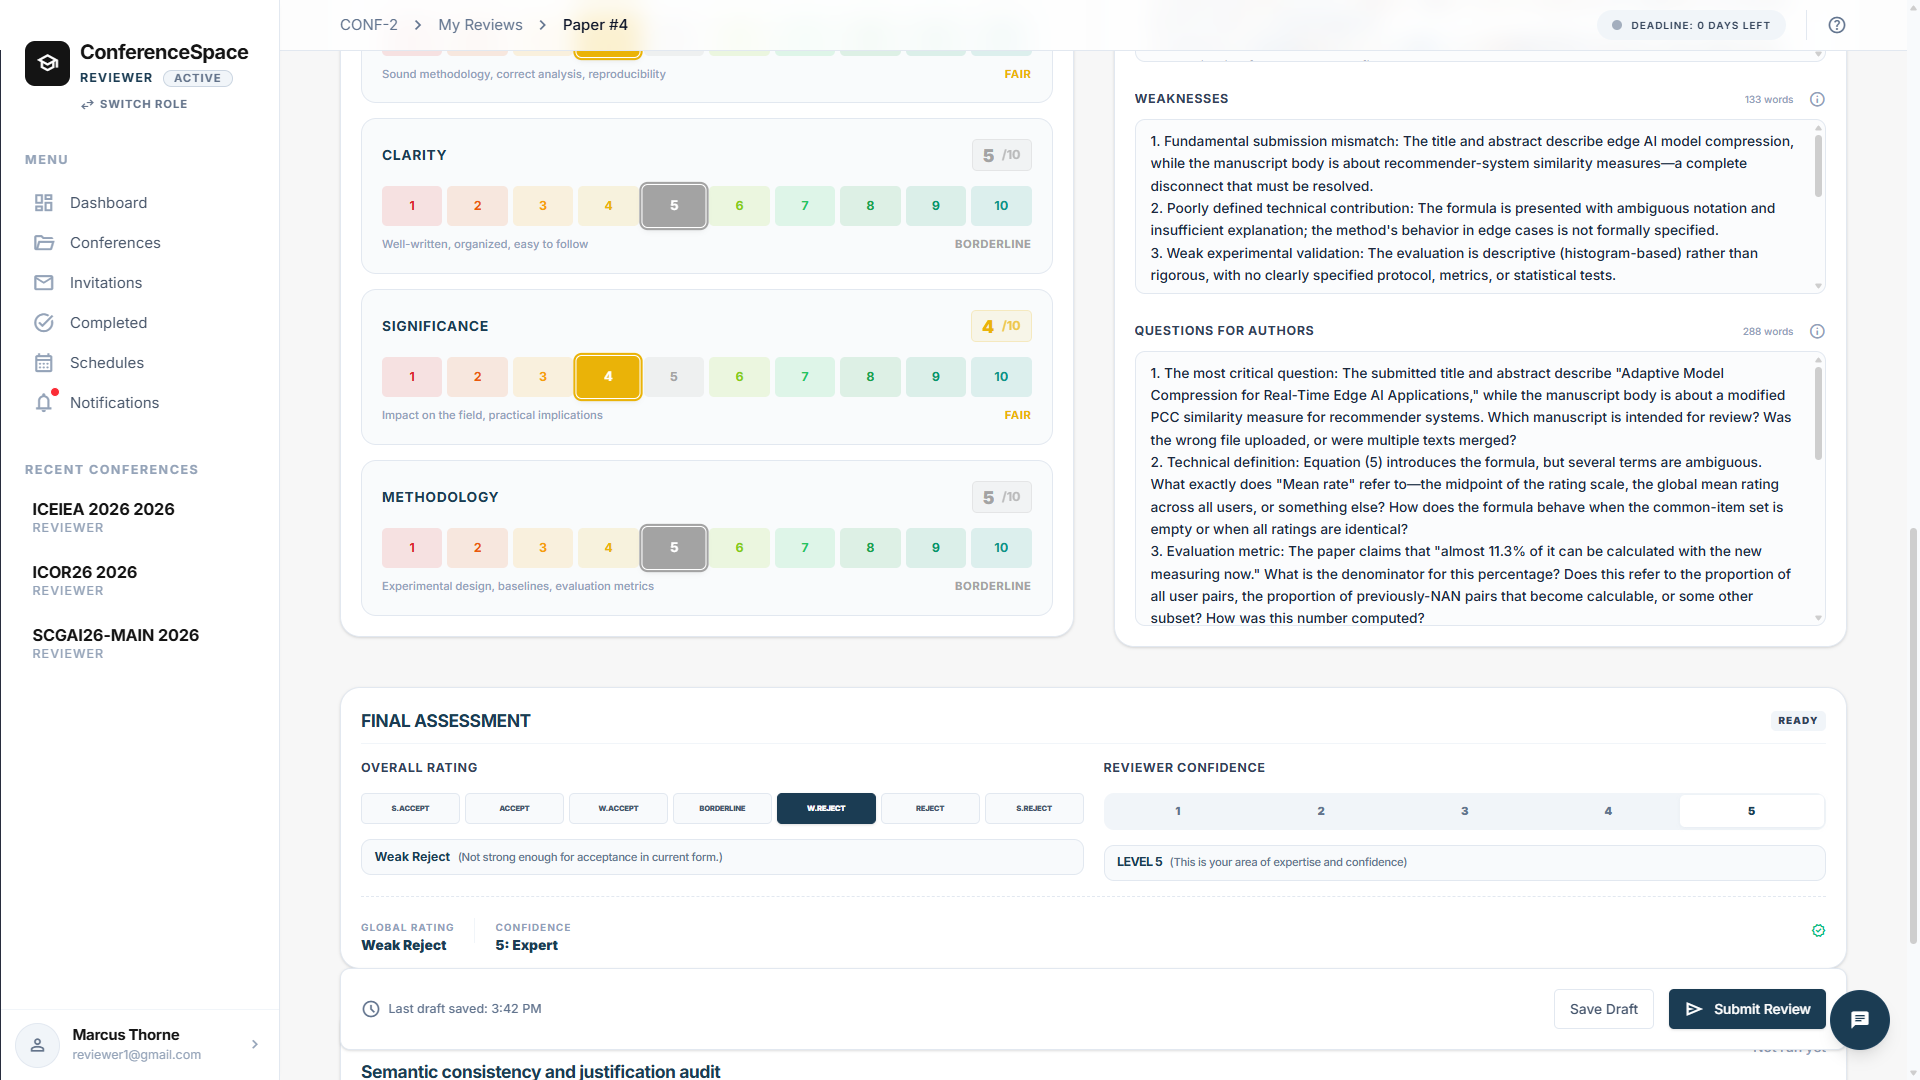
\includegraphics[width=0.95\textwidth]{images/chapter_3_uc05_reviewer_workspace_2.png}
  \caption{Không gian làm việc với biểu mẫu phản biện mở rộng của Phản biện viên}
  \label{fig:uc05-workspace-2-cut}
\end{figure}

Hình~\ref{fig:uc05-workspace-2-cut} trình bày một biến thể khác của không gian làm việc và biểu mẫu phản biện.

\begin{figure}[H]
  \centering
  \makebox[\textwidth][c]{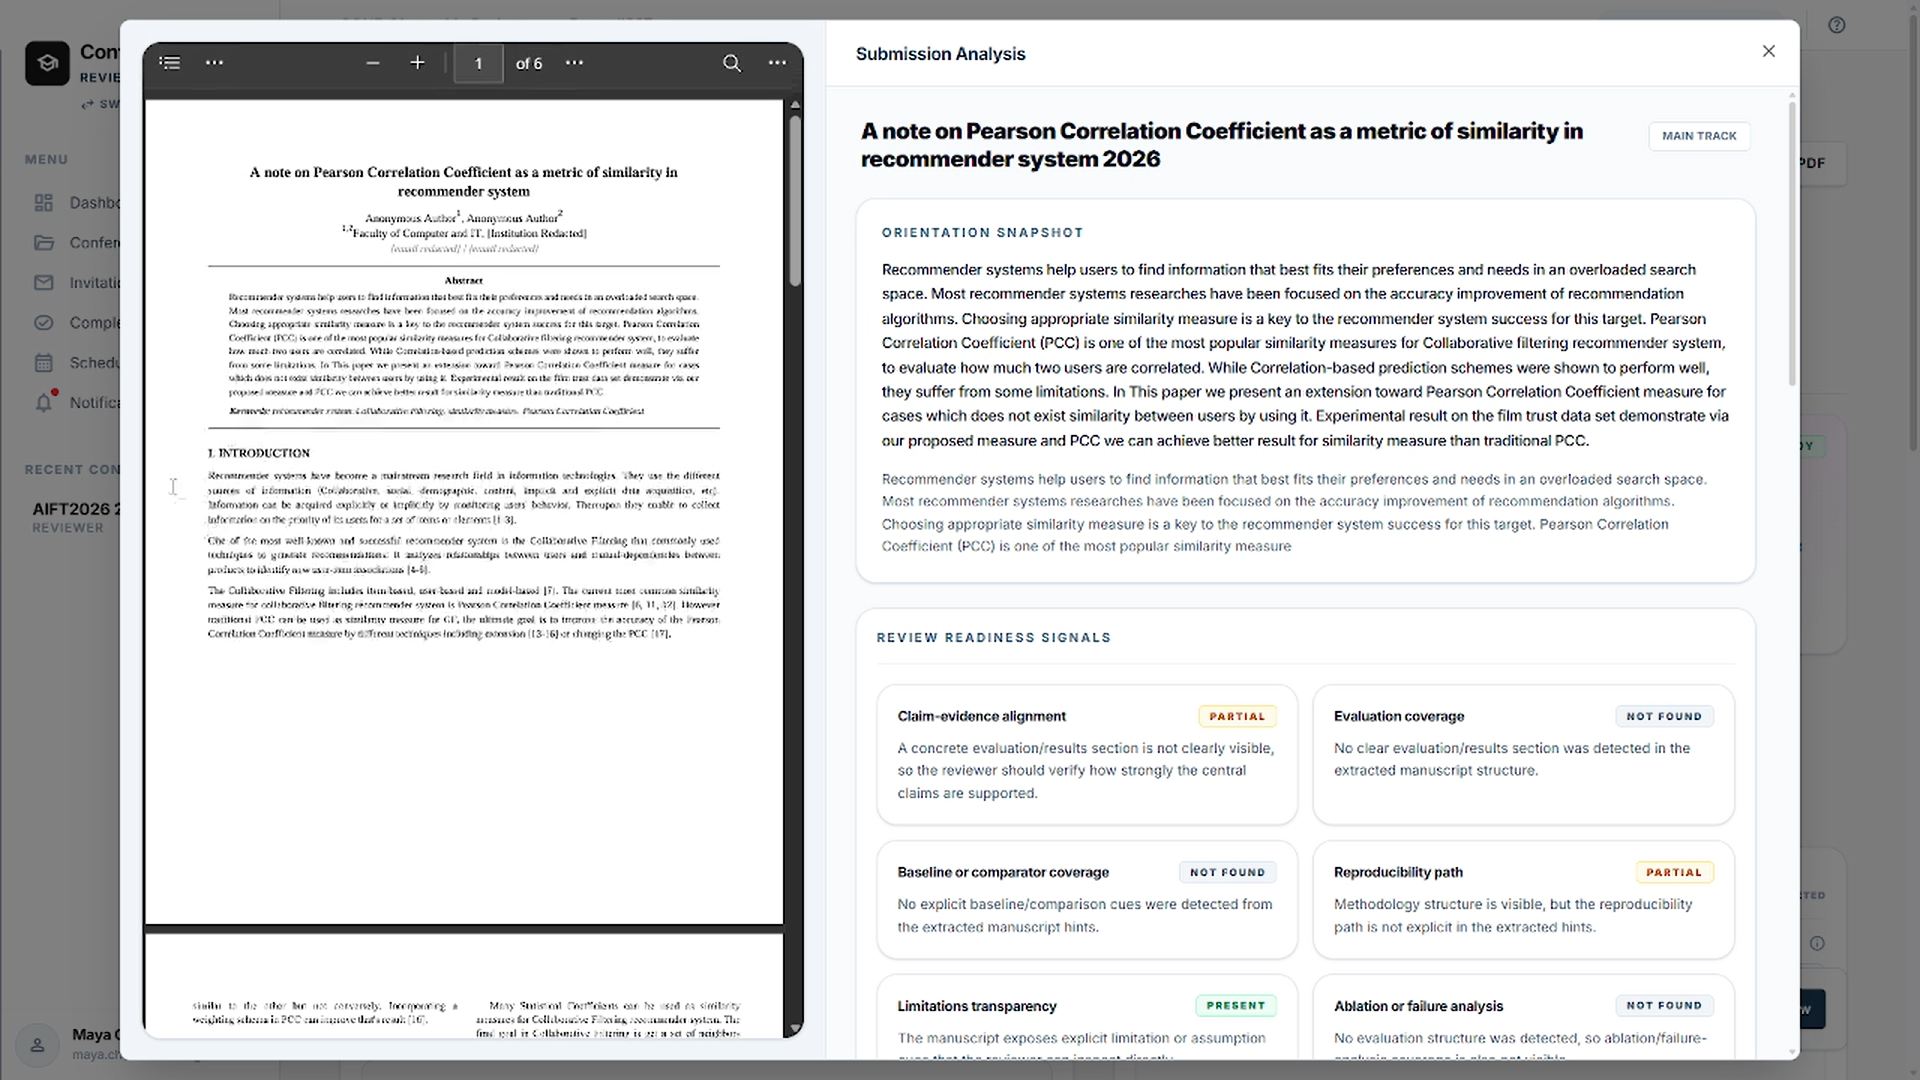
\includegraphics[width=1.10\textwidth]{images/chapter_3_uc05_reviewer_initial_analysis.png}}
  \caption{Bản định hướng đọc của Reviewer Initial Analysis}
  \label{fig:uc05-ria-cut}
\end{figure}

Hình~\ref{fig:uc05-ria-cut} thể hiện bản định hướng đọc do Reviewer Initial Analysis tạo ra để Phản biện viên tham khảo trước khi bắt đầu soạn phản biện.

\begin{figure}[H]
  \centering
  \makebox[\textwidth][c]{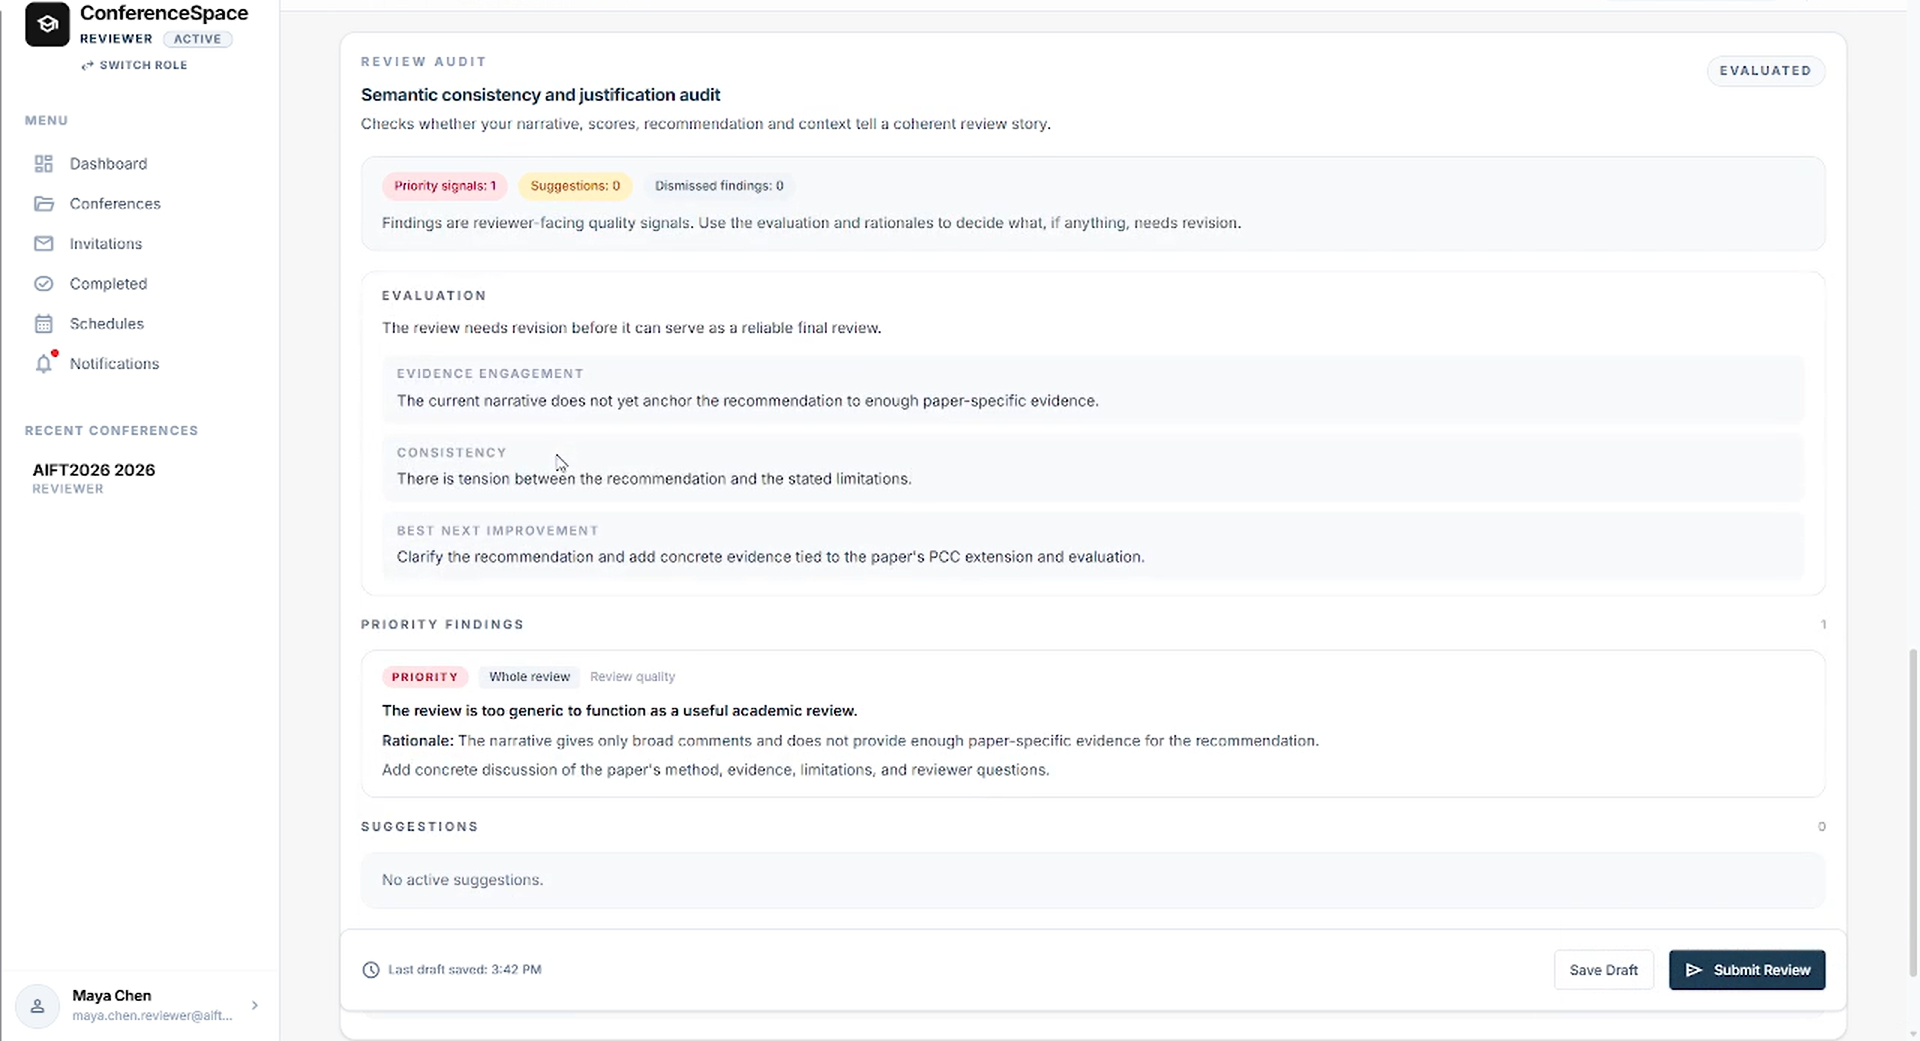
\includegraphics[width=1.10\textwidth]{images/chapter_3_uc05_reviewer_quality_auditor.png}}
  \caption{Bảng rà soát bản nháp của Review Quality Auditor}
  \label{fig:uc05-rqa-cut}
\end{figure}

Trước khi gửi phản biện, Phản biện viên xem bảng rà soát do Review Quality Auditor tạo ra tại Hình~\ref{fig:uc05-rqa-cut}.

Review Quality Auditor chạy trước khi gửi để đưa các phát hiện vào bảng rà soát. Phát hiện mức \textit{blocking} được làm nổi bật nhưng không ngăn Phản biện viên gửi phản biện. Nếu tác vụ rà soát không thể hoàn tất do lỗi dịch vụ, backend yêu cầu Phản biện viên xác nhận tiếp tục mà không có kết quả rà soát và ghi sự kiện này vào nhật ký. Hệ thống phân biệt phát hiện về chất lượng với lỗi không thể thực hiện bước rà soát: phát hiện chất lượng cung cấp thông tin để Phản biện viên xem xét, còn lỗi thực thi được thông báo rõ và ghi vào nhật ký.

\subsubsection{UC-06. Phân công phản biện có kiểm tra xung đột lợi ích}

Hệ thống chuẩn bị các cặp bài nộp--Phản biện viên, tính điểm phù hợp, loại các cặp có xung đột lợi ích khỏi đề xuất tự động và theo dõi số phân công được tạo trong cùng lượt chạy. Trước khi điều chỉnh hoặc xác nhận, Chủ tọa xem điểm số, lý do đối sánh, trạng thái kiểm tra xung đột lợi ích, tải phát sinh trong lượt chạy và danh sách bài chưa đủ Phản biện viên. Phản hồi \CodeBreak{AutoAssignResponse} không liệt kê đầy đủ từng cặp ứng viên bị loại. Khi Chủ tọa thêm đề xuất thủ công, backend kiểm tra quyền và trả cảnh báo xung đột lợi ích nhưng hiện chưa ngăn lưu; vì vậy, Chủ tọa phải xử lý cảnh báo trước khi xác nhận phương án.

\begin{figure}[H]
  \centering
  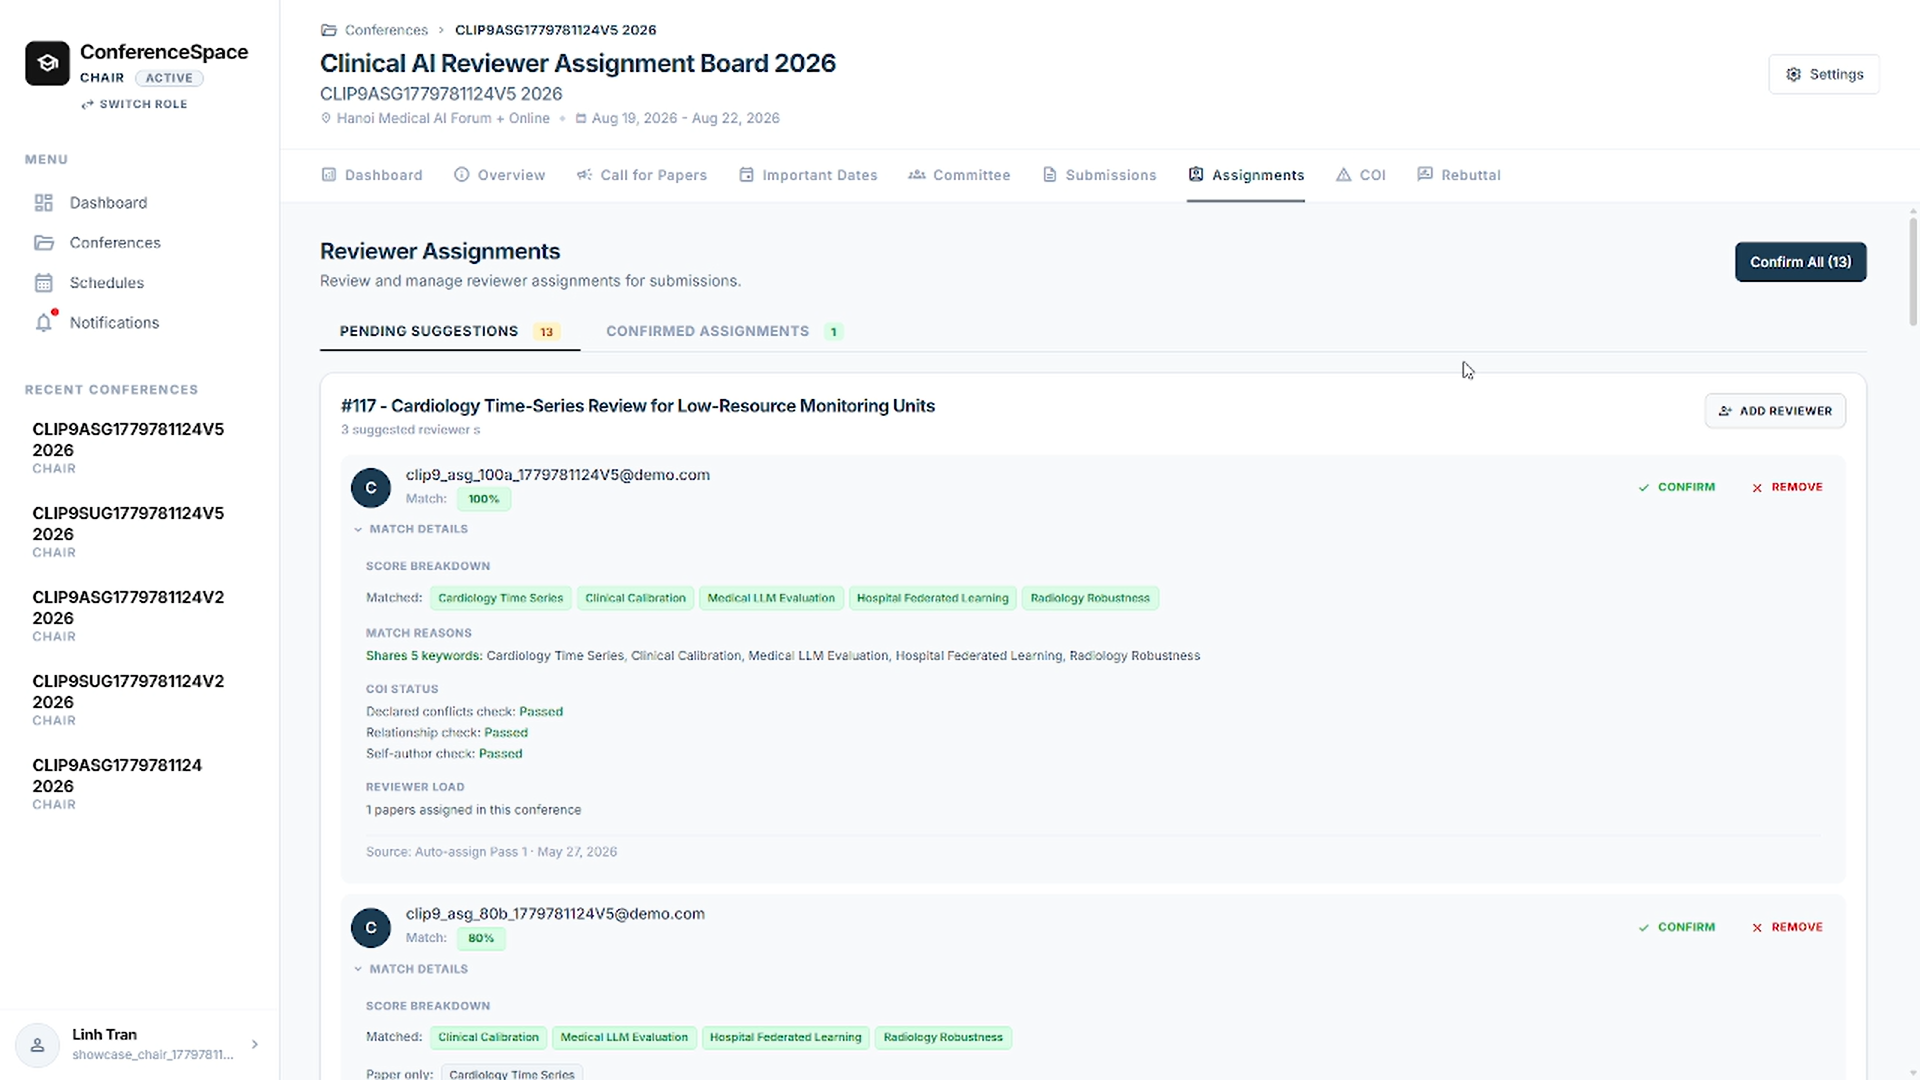
\includegraphics[width=0.95\textwidth]{images/chapter_3_uc06_assignment_dashboard.png}
  \caption{Giao diện bảng điều khiển quản lý phân công phản biện của Chủ tọa}
  \label{fig:uc06-dashboard-cut}
\end{figure}

Hình~\ref{fig:uc06-dashboard-cut} minh họa bảng điều khiển quản lý phân công phản biện của Chủ tọa.

\begin{figure}[H]
  \centering
  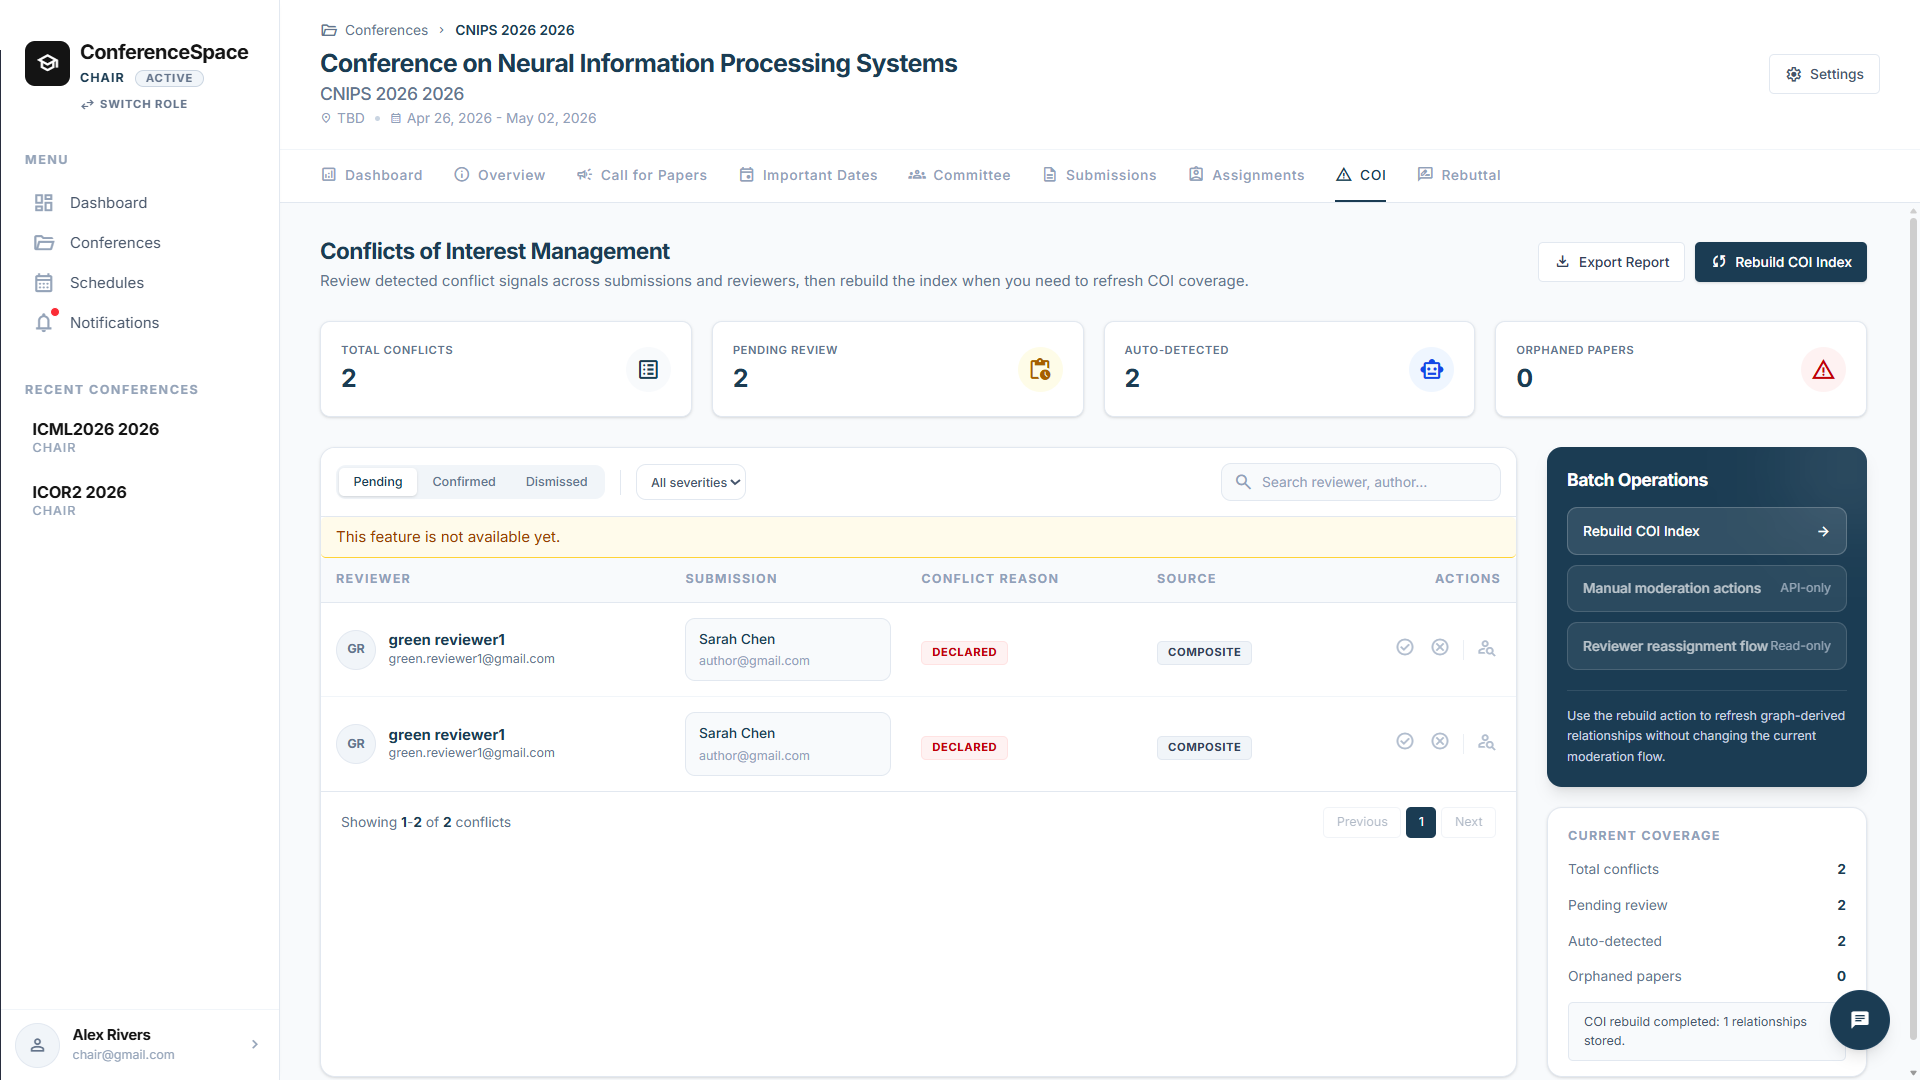
\includegraphics[width=0.95\textwidth]{images/chapter_3_uc06_coi_verification.png}
  \caption{Giao diện kiểm tra xung đột lợi ích giữa phản biện viên và bài nộp}
  \label{fig:uc06-coi-verification-cut}
\end{figure}

Hình~\ref{fig:uc06-coi-verification-cut} minh họa giao diện kiểm tra xung đột lợi ích giữa phản biện viên và bài nộp.

\begin{figure}[H]
  \centering
  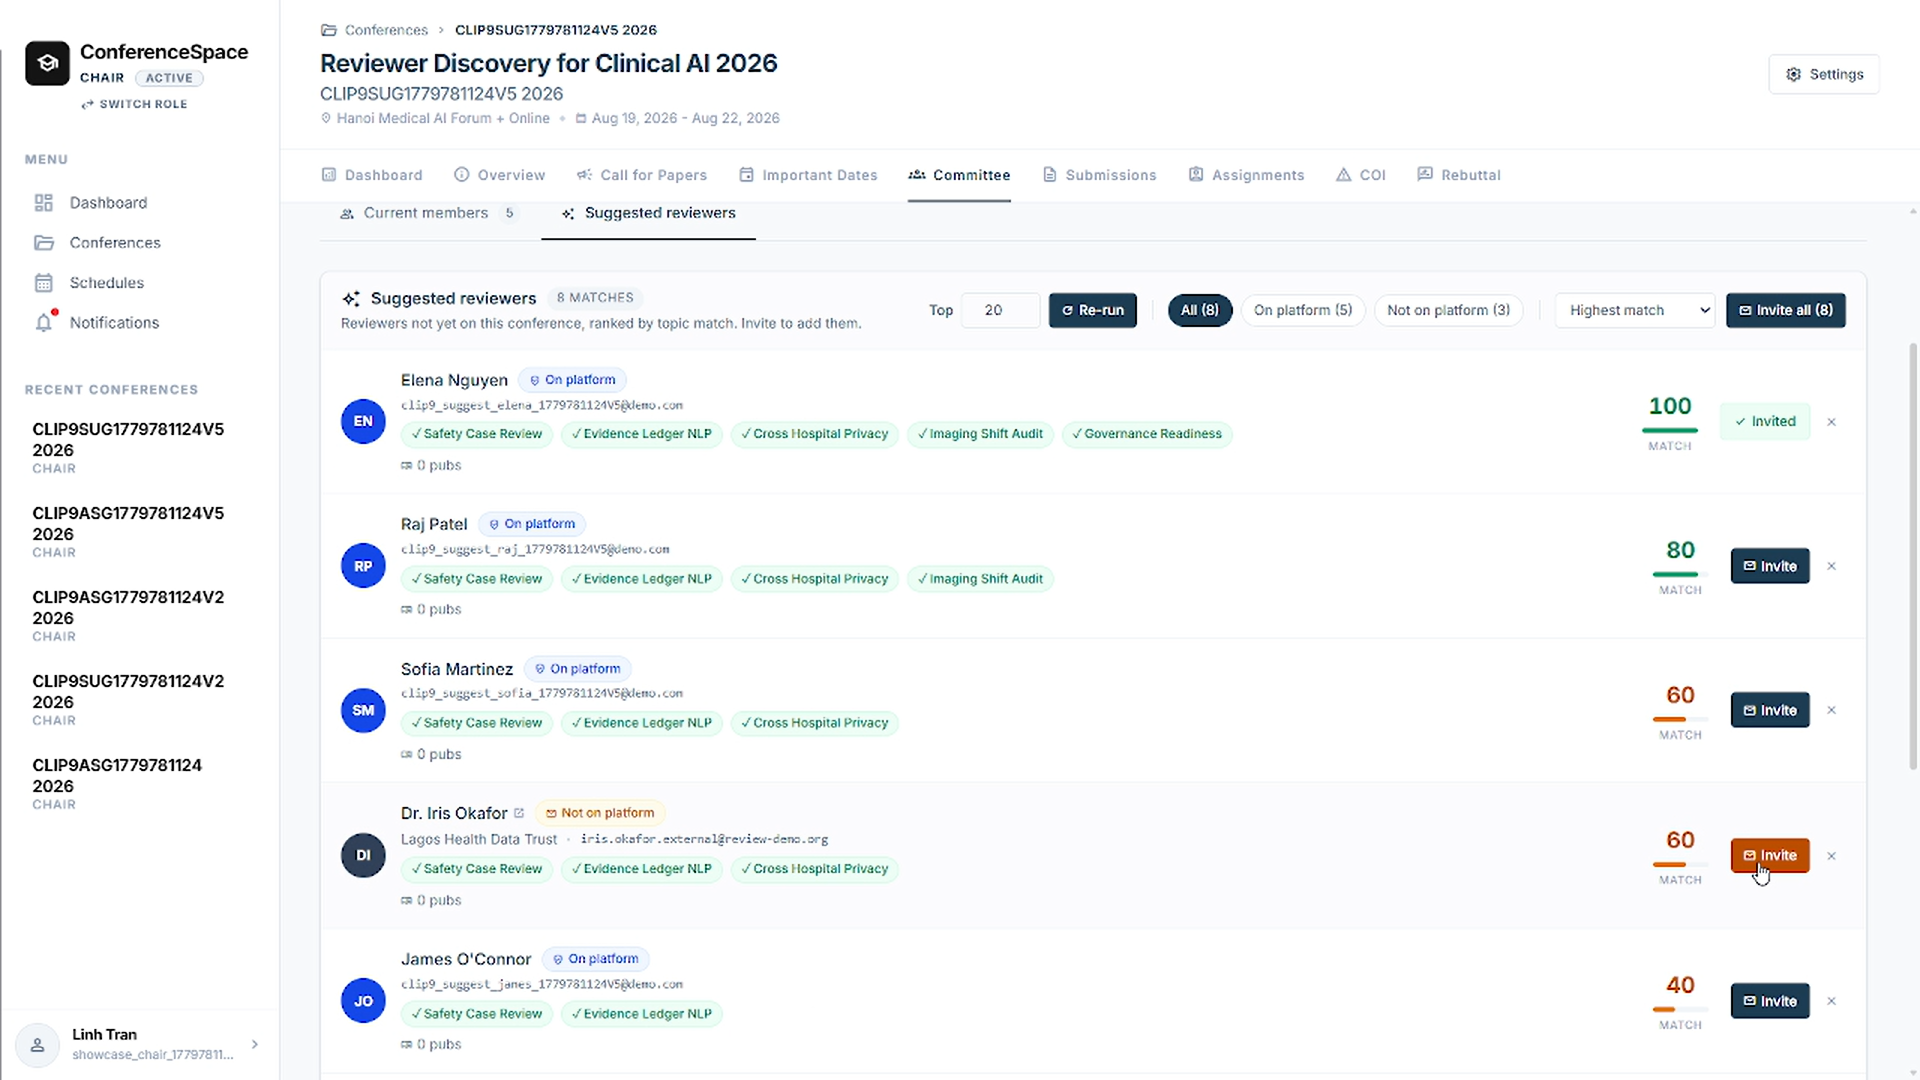
\includegraphics[width=0.95\textwidth]{images/chapter_3_uc06_assignment_suggestions.png}
  \caption{Danh sách đề xuất đối sánh và điểm phù hợp để Chủ tọa xem xét}
  \label{fig:uc06-suggestions-cut}
\end{figure}

Hình~\ref{fig:uc06-suggestions-cut} liệt kê các đề xuất đối sánh cùng điểm phù hợp để Chủ tọa xem xét trước khi xác nhận.

Công thức tính điểm, thủ tục phân công, lượt dự phòng và các trường hợp ngoại lệ được trình bày tại Mục~\ref{subsec:ch3-matching-cut}. Thuật toán tự động không nới ràng buộc xung đột lợi ích, kể cả khi hệ thống không tìm được đủ Phản biện viên; luồng thêm đề xuất thủ công hiện dùng cảnh báo thay cho cưỡng chế tại thời điểm ghi dữ liệu.

\subsubsection{UC-07. Quản lý hội nghị và theo dõi tiến độ}

Chủ tọa cấu hình thông tin hội nghị, chuyên đề, hạn chót nộp bài, biểu mẫu phản biện và chính sách; mời thành viên hội đồng chương trình; theo dõi số bài, tiến độ phản biện và các trường hợp cần xử lý. Hệ thống từ chối cấu hình thiếu trường bắt buộc, hạn chót nộp bài không hợp lệ hoặc thao tác của người dùng không có quyền. Bảng điều khiển hỗ trợ nhận biết các trường hợp cần xử lý nhưng không tự chuyển giai đoạn hoặc ra quyết định thay Chủ tọa.

\begin{figure}[H]
  \centering
  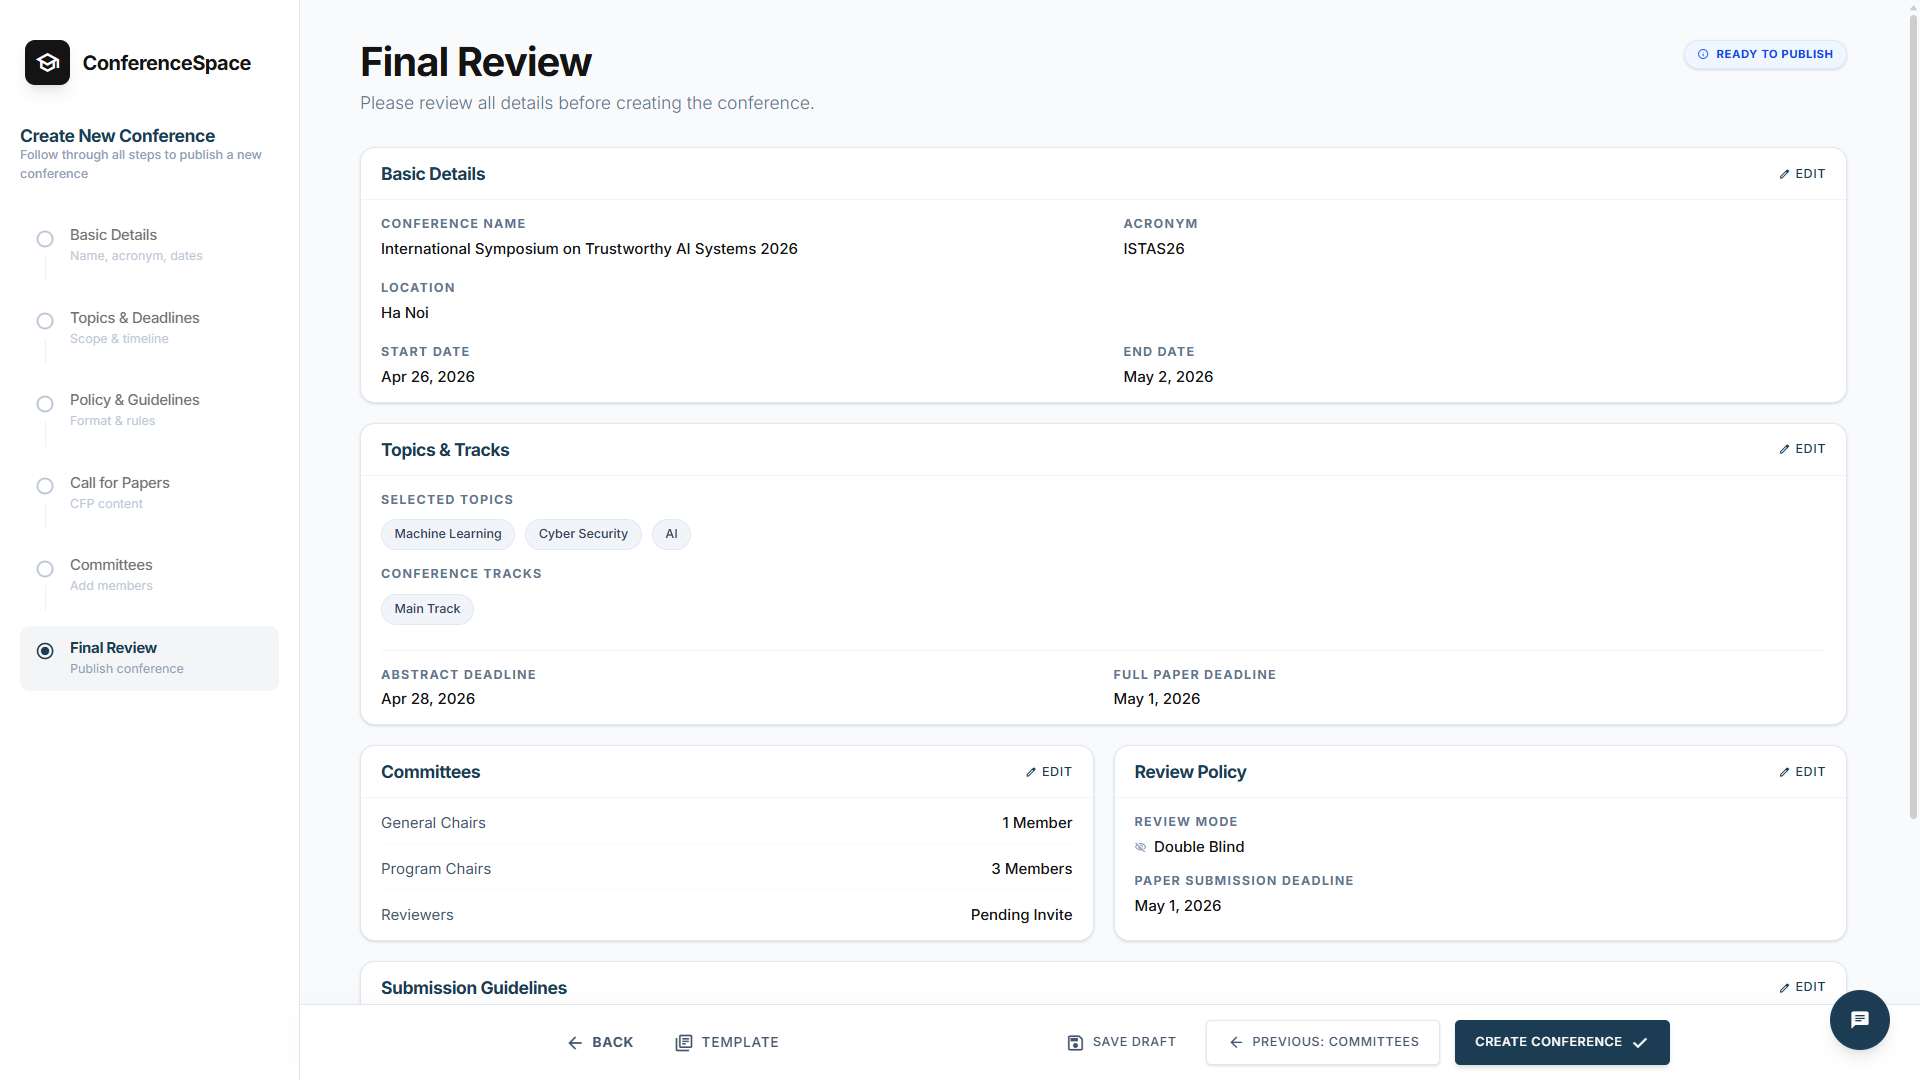
\includegraphics[width=0.95\textwidth]{images/chapter_3_uc07_conference_config.png}
  \caption{Giao diện thiết lập cấu hình thông tin và hạn chót nộp bài hội nghị của Chủ tọa}
  \label{fig:uc07-config-cut}
\end{figure}

Hình~\ref{fig:uc07-config-cut} thể hiện giao diện thiết lập cấu hình thông tin và hạn chót nộp bài hội nghị.

\begin{figure}[H]
  \centering
  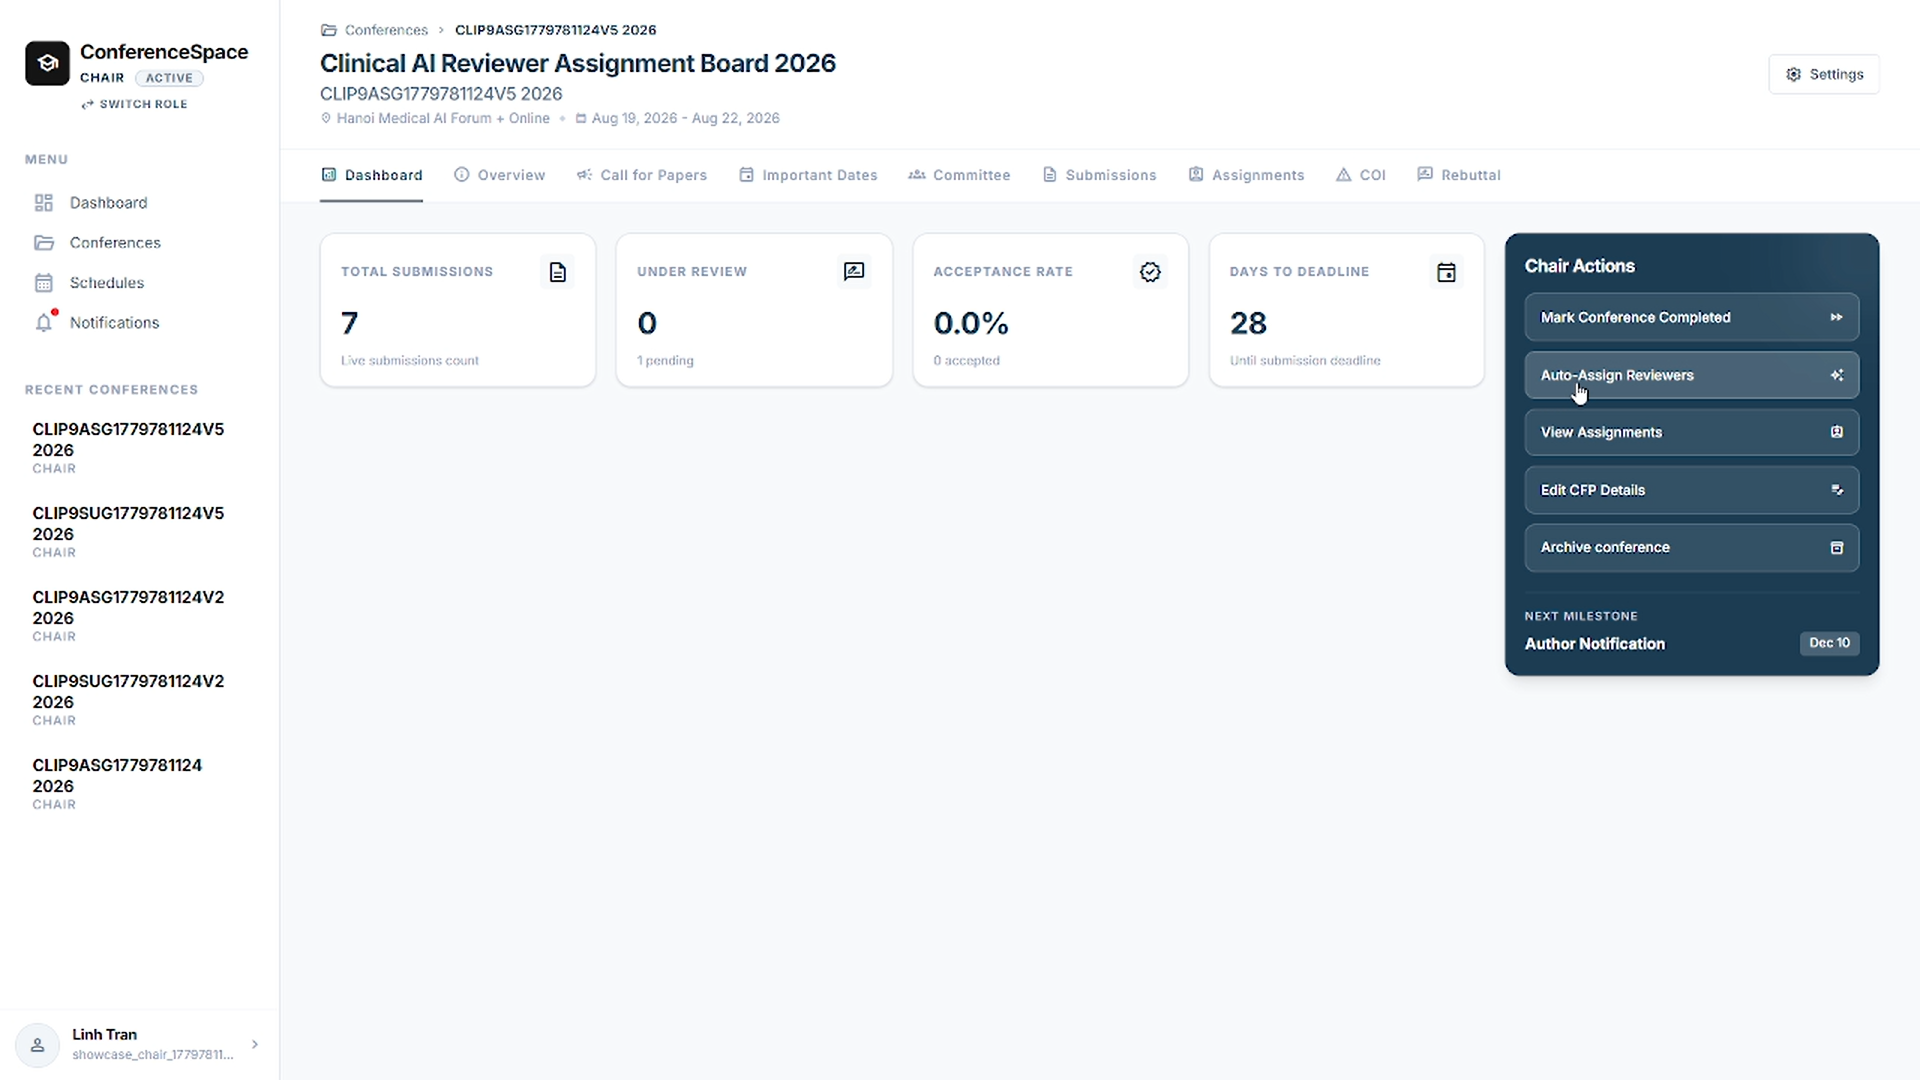
\includegraphics[width=0.95\textwidth]{images/chapter_3_uc07_chair_dashboard.png}
  \caption{Bảng điều khiển tiến độ hội nghị của Chủ tọa}
  \label{fig:uc07-dashboard-cut}
\end{figure}

Hình~\ref{fig:uc07-dashboard-cut} cung cấp cái nhìn tổng quan về hoạt động điều phối, bổ sung cho các hình chuyên biệt về đối sánh và hỗ trợ quyết định.

\begin{figure}[H]
  \centering
  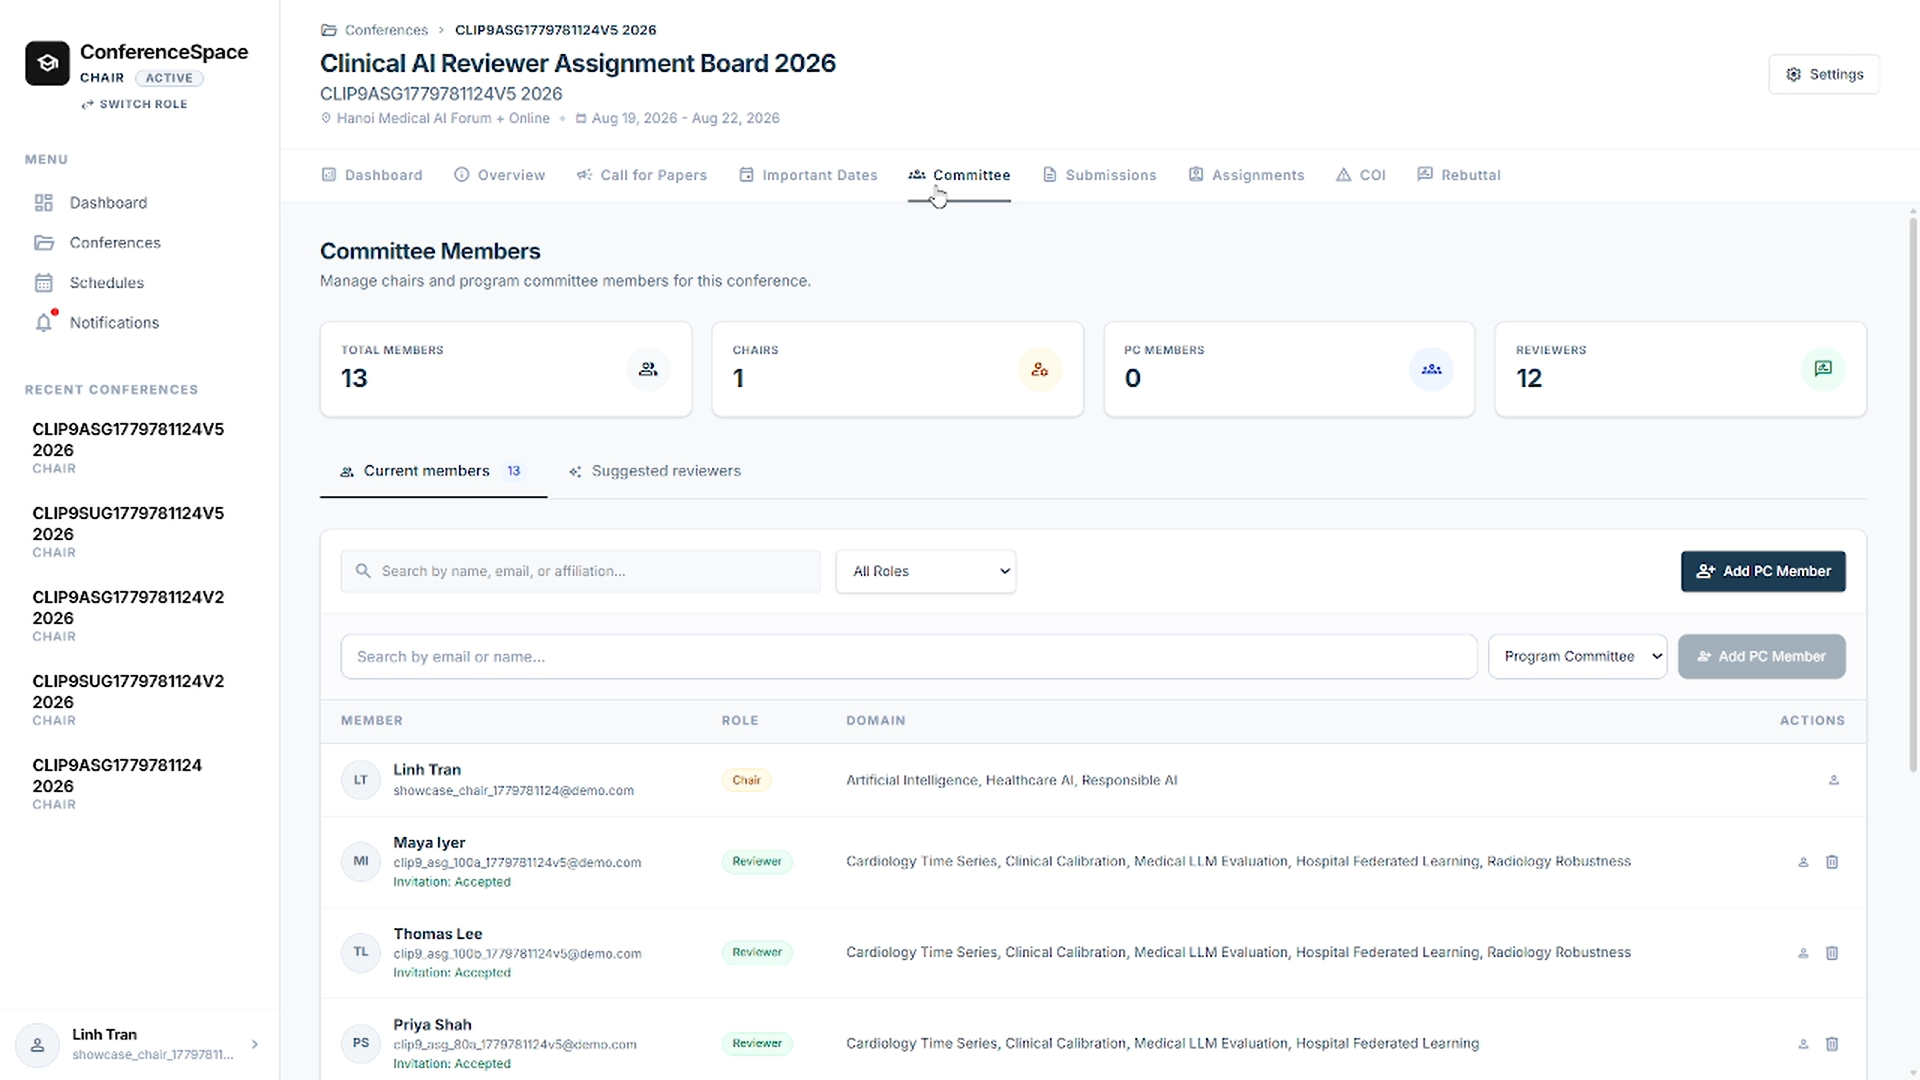
\includegraphics[width=0.95\textwidth]{images/chapter_3_uc07_committee_management.png}
  \caption{Giao diện quản lý ban chương trình và trạng thái lời mời phản biện viên}
  \label{fig:uc07-committee-cut}
\end{figure}

Hình~\ref{fig:uc07-committee-cut} minh họa giao diện quản lý ban chương trình và trạng thái lời mời phản biện viên.

\subsubsection{UC-08. Trao đổi theo bài nộp}

Chủ tọa hoặc Đồng chủ tọa mở giai đoạn phản hồi và kết thúc giai đoạn này trước khi ra quyết định; giai đoạn thảo luận chỉ được mở khi cấu hình hội nghị cho phép. Phản biện viên được phân công có thể tạo chuỗi thảo luận. Tác giả của bài và Phản biện viên trao đổi trong chuỗi tương ứng, còn Chủ tọa xem toàn bộ lịch sử ở chế độ giám sát. Sau khi đọc phản hồi, Phản biện viên có thể cập nhật điểm, khuyến nghị và nhận xét của bài mình phụ trách. Backend kiểm tra quan hệ giữa người dùng, bài nộp và chuỗi thảo luận trước mỗi thao tác. Nội dung trao đổi cùng đánh giá cập nhật được lưu với bài nộp và trở thành nguồn bằng chứng cho Chair Decision Copilot.

\begin{figure}[H]
  \centering
  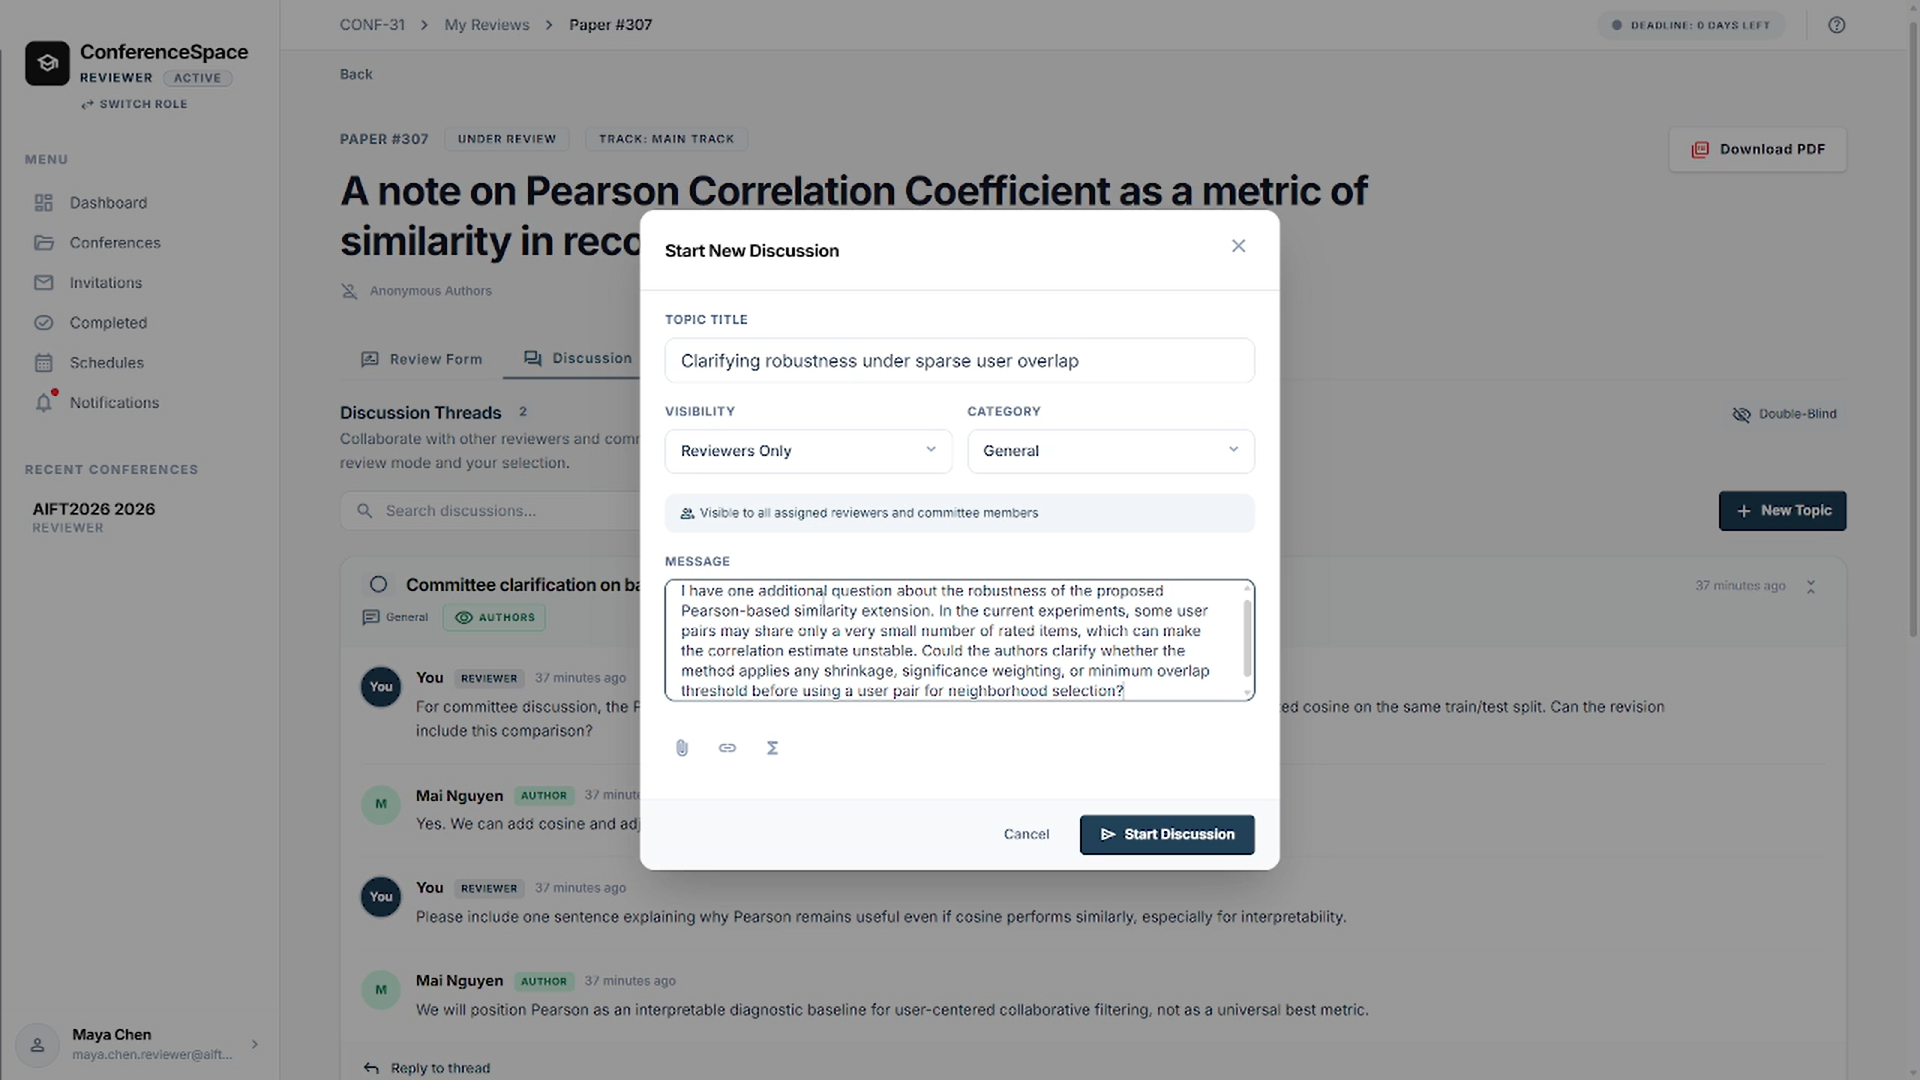
\includegraphics[width=0.95\textwidth]{images/chapter_3_uc08_create_discussion.png}
  \caption{Giao diện khởi tạo chủ đề thảo luận mới cho bài nộp}
  \label{fig:uc08-create-discussion-cut}
\end{figure}

Hình~\ref{fig:uc08-create-discussion-cut} minh họa giao diện khởi tạo chủ đề thảo luận mới cho bài nộp.

\begin{figure}[H]
  \centering
  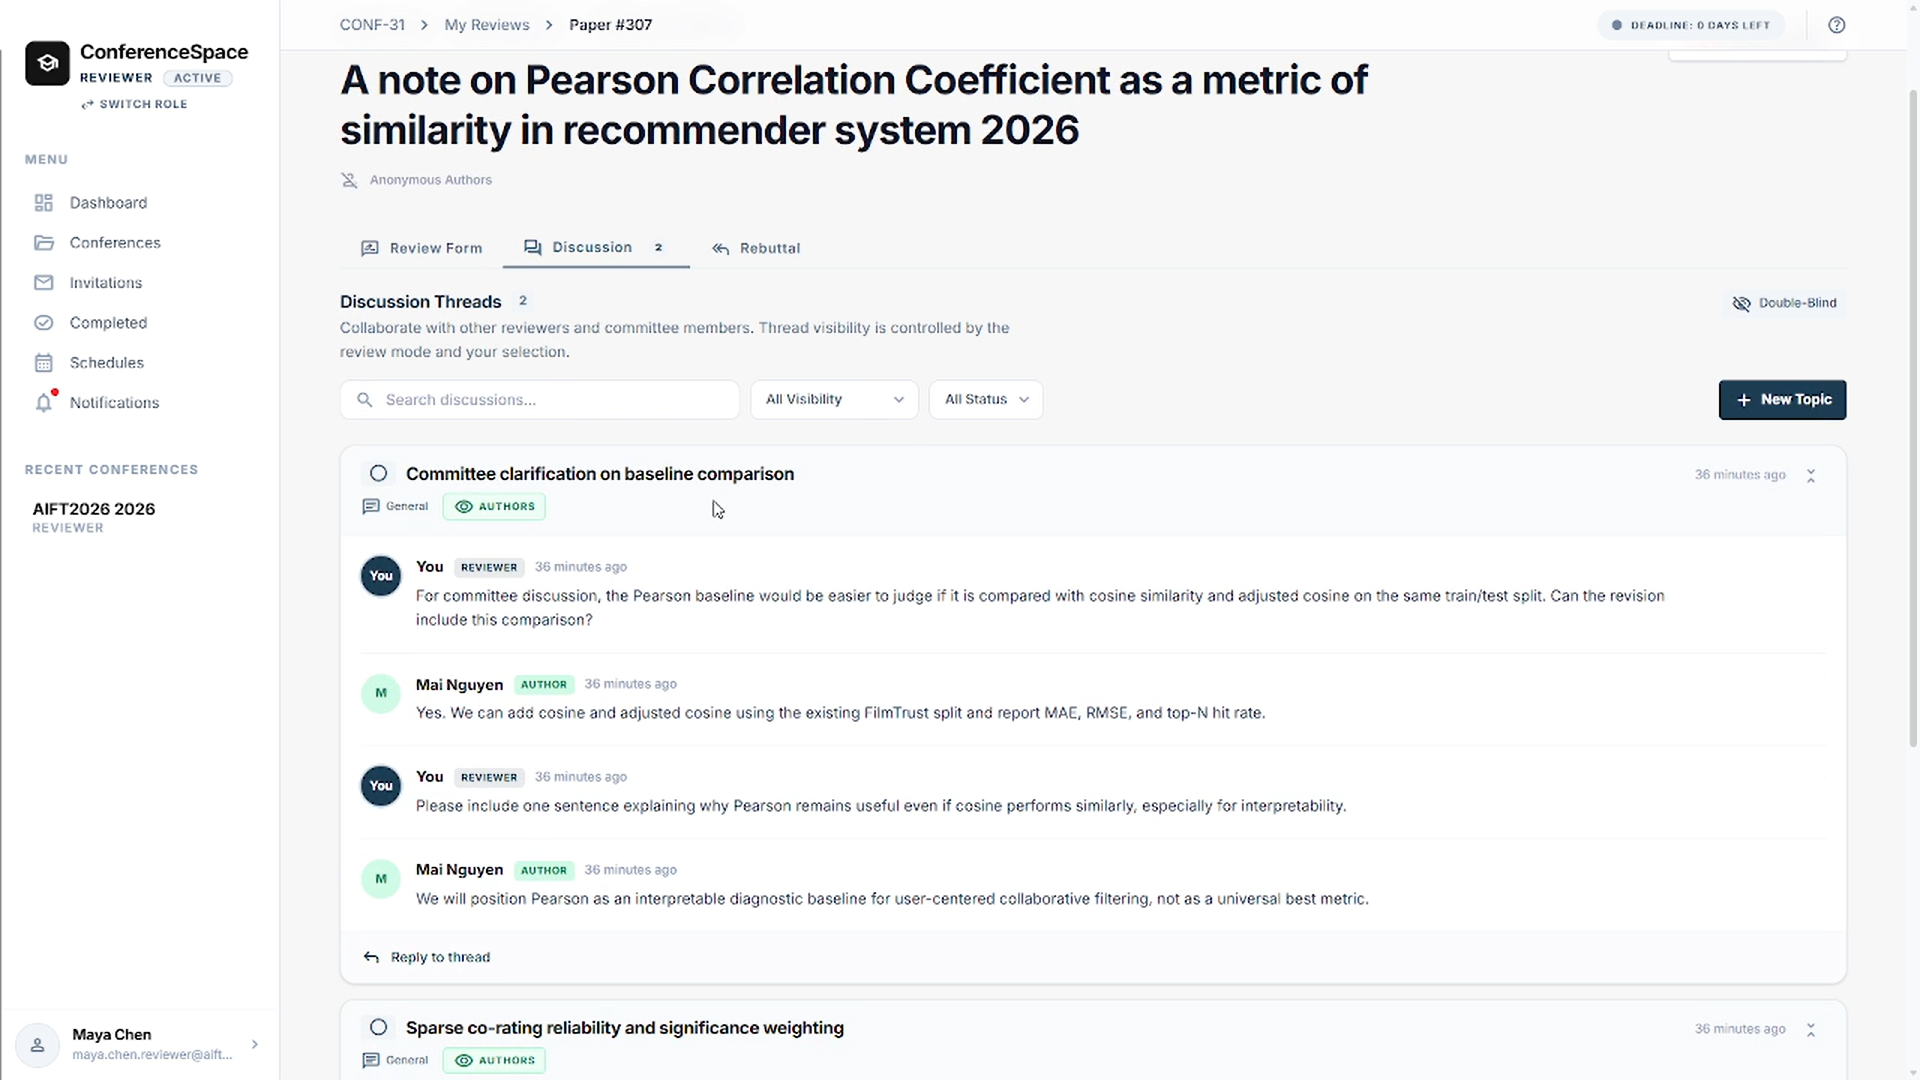
\includegraphics[width=0.95\textwidth]{images/chapter_3_uc08_discussion_chat.png}
  \caption{Giao diện hiển thị danh sách và trao đổi nội dung thảo luận}
  \label{fig:uc08-discussion-chat-cut}
\end{figure}

Hình~\ref{fig:uc08-discussion-chat-cut} thể hiện giao diện hiển thị danh sách chủ đề và nội dung trao đổi trong từng chủ đề.

\subsubsection{UC-09. Tổng hợp bằng chứng hỗ trợ Chủ tọa ra quyết định}

Backend tập hợp điểm số, bản phản biện, phản hồi của Tác giả, thay đổi sau phản hồi và nội dung thảo luận. Chair Decision Copilot tổ chức các nguồn này thành bản tổng hợp gồm điểm đồng thuận, bất đồng, vấn đề còn mở và bằng chứng liên quan. Chủ tọa đối chiếu bản tổng hợp với dữ liệu gốc rồi tự ghi nhận quyết định cuối cùng. Khi bộ bằng chứng thay đổi, hệ thống đánh dấu kết quả cũ là không còn hiệu lực.

\begin{figure}[H]
  \centering
  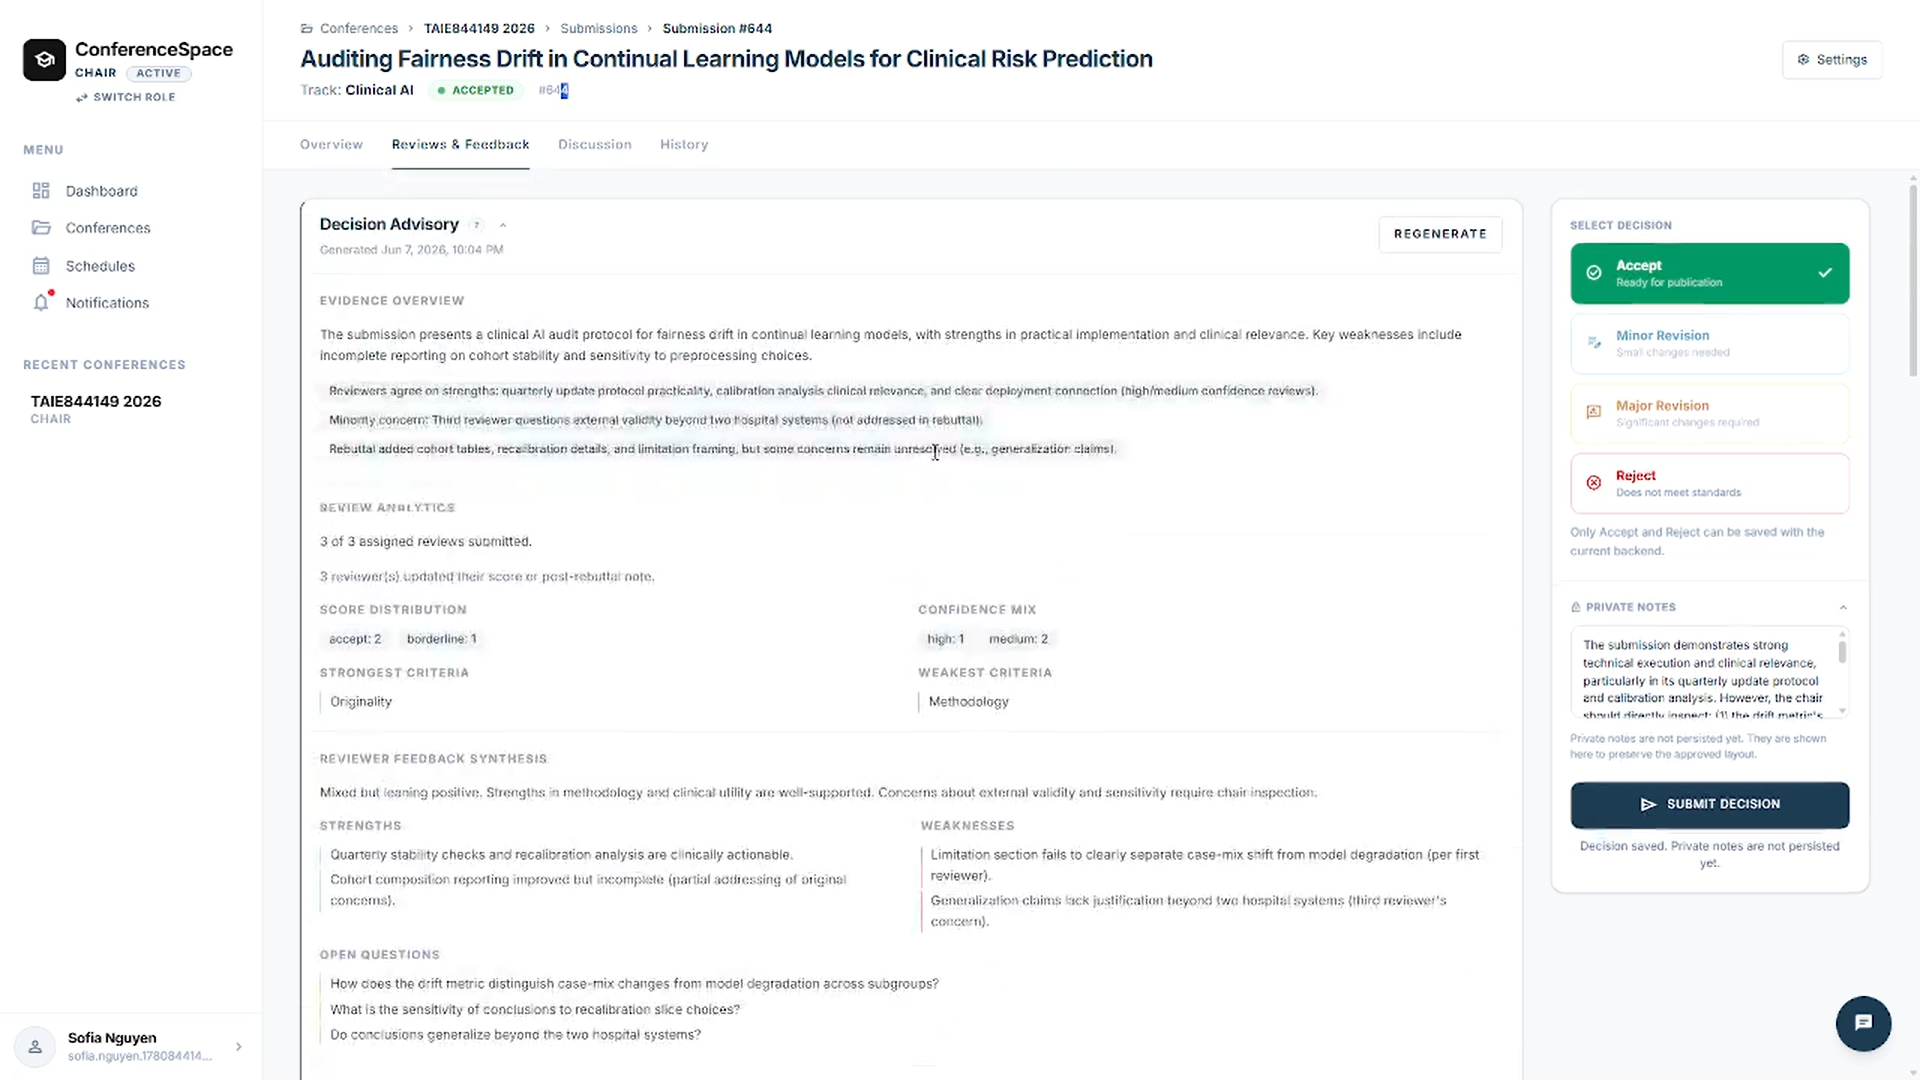
\includegraphics[width=0.95\textwidth]{images/chapter_3_uc09_decision_support.png}
  \caption{Giao diện tổng hợp bằng chứng và ghi nhận quyết định của Chủ tọa}
  \label{fig:uc09-decision-cut}
\end{figure}

Hình~\ref{fig:uc09-decision-cut} minh họa giao diện tổng hợp bằng chứng và ghi nhận quyết định của Chủ tọa.

Chair Decision Copilot không tạo khuyến nghị chấp nhận hoặc từ chối. Khi dịch vụ AI gặp lỗi, Chủ tọa vẫn có thể đọc trực tiếp các nguồn bằng chứng và tiếp tục quy trình nghiệp vụ.

\subsubsection{UC-10. Truy vấn trạng thái và hướng dẫn theo ngữ cảnh bằng Chatbot Agent}

Chatbot Agent nhận câu hỏi, lịch sử hội thoại và ngữ cảnh trang hiện tại. Nếu câu hỏi cần dữ liệu nghiệp vụ, Chatbot Agent gọi công cụ truy vấn để gửi yêu cầu có cấu trúc đến backend; backend kiểm tra mã xác thực, tài nguyên, trường dữ liệu, bộ lọc và quyền của người dùng trước khi trả phần dữ liệu tối thiểu được phép. Chatbot Agent dùng kết quả này để tạo câu trả lời phù hợp với vai trò và không truy cập trực tiếp cơ sở dữ liệu.

Backend từ chối yêu cầu vượt quá quyền truy cập; Chatbot Agent thông báo rõ khi câu hỏi nằm ngoài phạm vi chức năng được hỗ trợ. Khi công cụ gặp lỗi, hệ thống trả trạng thái lỗi thay vì tạo dữ liệu không có căn cứ. Các kịch bản hội thoại ở Chương 4 kiểm tra ranh giới này trong phạm vi tài nguyên và vai trò đã chọn.

\begin{figure}[H]
  \centering
  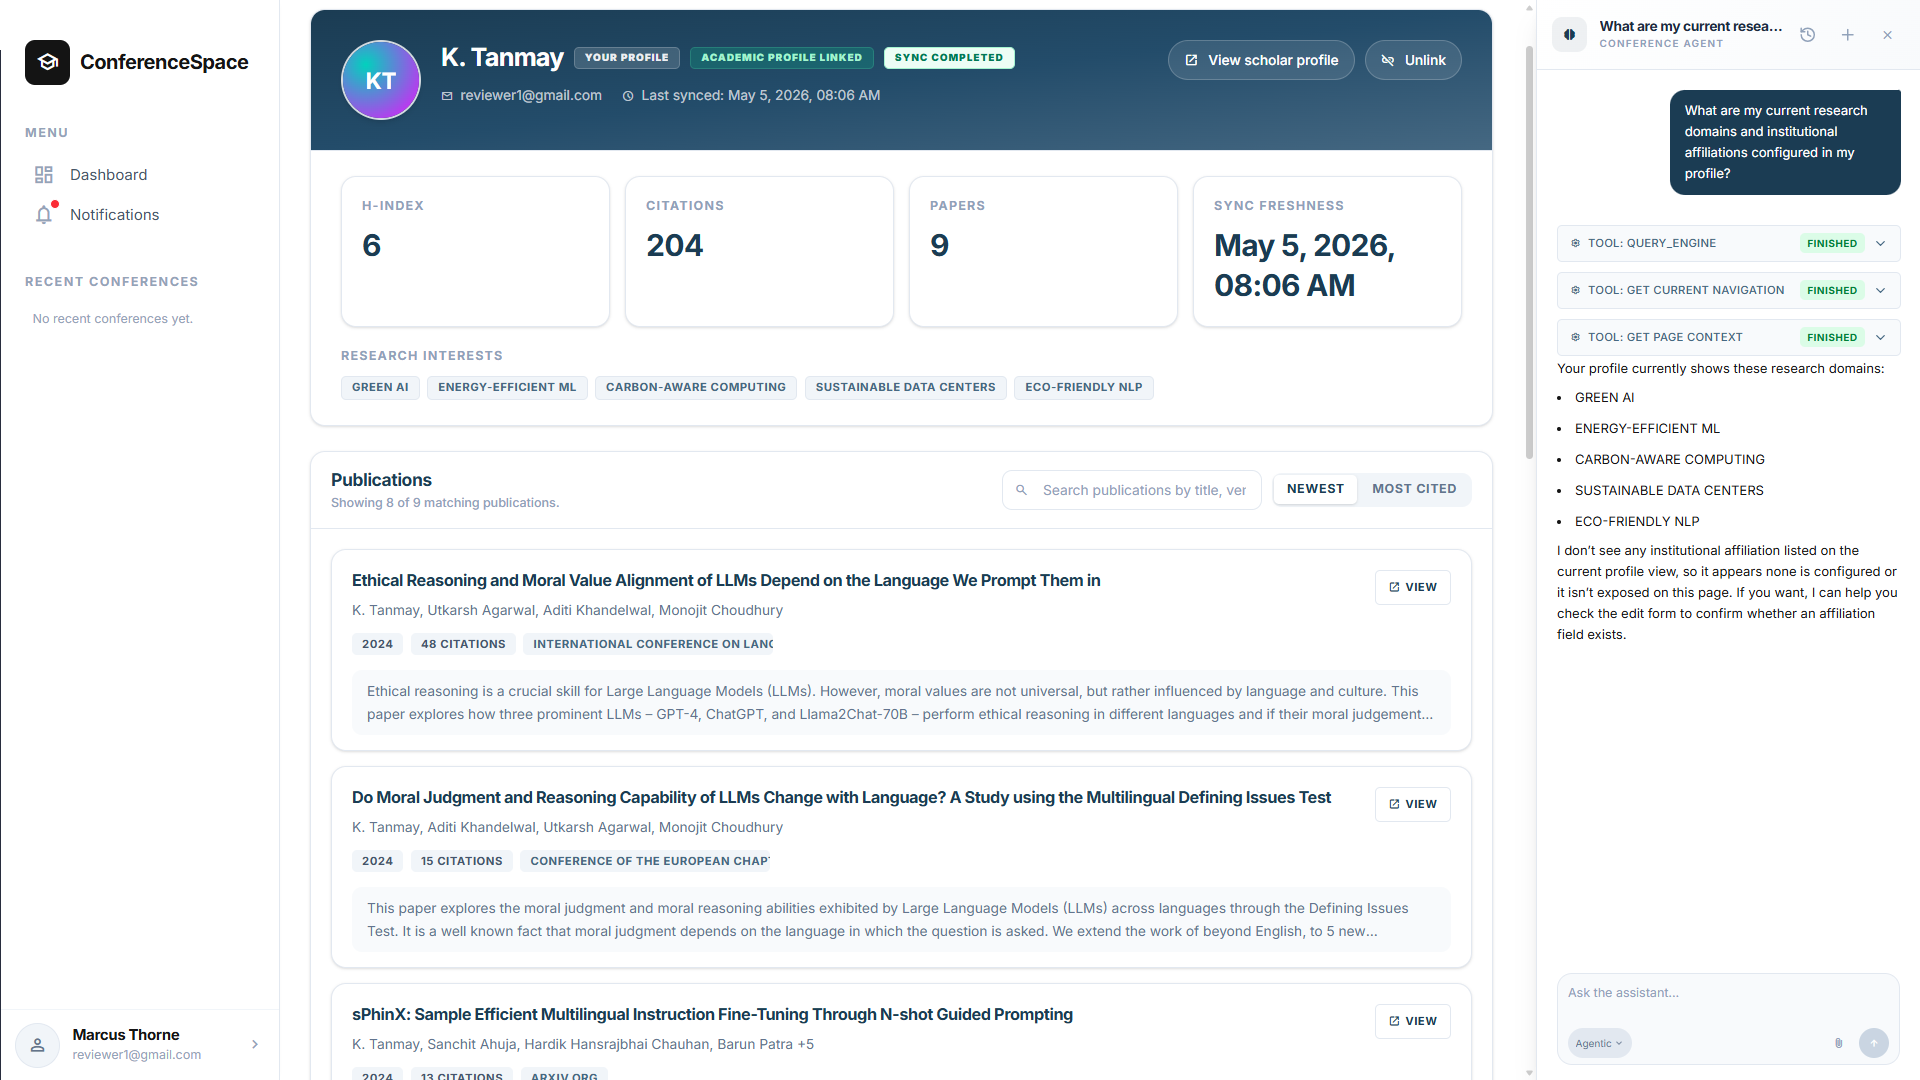
\includegraphics[width=0.95\textwidth]{images/chapter_3_uc10_chatbot_interface.png}
  \caption{Giao diện hội thoại và hỗ trợ tra cứu thông tin của Chatbot Agent}
  \label{fig:uc10-chatbot-cut}
\end{figure}

Hình~\ref{fig:uc10-chatbot-cut} minh họa giao diện hội thoại của Chatbot Agent trong luồng này.

\section{Thiết kế kỹ thuật}

\subsection{Kiến trúc tổng thể}
\label{subsec:ch3-architecture-cut}

ConferenceSpace gồm giao diện web Next.js, backend Go/Gin, dịch vụ AI FastAPI, PostgreSQL, Redis, Neo4j và cổng Caddy. Backend nghiệp vụ là một ứng dụng nguyên khối có kiến trúc phân lớp; nhóm không chia nhỏ nghiệp vụ thành các vi dịch vụ khi chưa có nhu cầu vận hành tương ứng. Dịch vụ AI và các kho dữ liệu được tách tại ranh giới triển khai vì có vòng đời, tải xử lý và yêu cầu truy cập khác với backend.

\begin{figure}[H]
  \centering
  \begin{adjustbox}{max width=\textwidth}
    \begin{tikzpicture}[node distance=12mm and 18mm, >=Latex]
      \node[prismNode] (browser) at (0,0) {Trình duyệt};
      \node[prismNode] (caddy) at (0,-2.2) {Caddy};
      \node[prismNode] (web) at (0,-4.4) {Next.js};
      \node[prismNode] (backend) at (0,-6.6) {Backend Go/Gin};
      \node[prismNode] (postgres) at (-6.4,-9.2) {PostgreSQL};
      \node[prismNode] (neo4j) at (-2.1,-9.2) {Neo4j};
      \node[prismNode] (ai) at (2.1,-9.2) {Dịch vụ AI};
      \node[prismNode] (external) at (6.4,-9.2) {Nguồn dữ liệu học thuật bên ngoài};
      \node[prismNode] (redis) at (0,-11.8) {Redis};
      \node[prismNode] (model) at (4.3,-11.8) {Nhà cung cấp mô hình};
      \draw[prismArrow] (browser) -- (caddy);
      \draw[prismArrow] (caddy) -- (web);
      \draw[prismArrow] (web) -- (backend);
      \draw[prismArrow] (web) -- node[prismEdgeLabel] {API hội thoại} (ai);
      \draw[prismArrow] (backend) -- (postgres);
      \draw[prismArrow] (backend) -- (neo4j);
      \draw[prismArrow] (backend) -- (ai);
      \draw[prismDashedArrow, bend left=24] (ai) to node[prismEdgeLabel] {endpoint truy vấn của backend} (backend);
      \draw[prismArrow] (backend) -- (external);
      \draw[prismArrow] (ai) -- (redis);
      \draw[prismArrow] (ai) -- (model);
      \draw[prismDashedArrow] (ai) -- node[prismEdgeLabel] {kết quả cần truy vết} (postgres);
    \end{tikzpicture}
  \end{adjustbox}
  \caption{Kiến trúc dịch vụ và ranh giới dữ liệu của ConferenceSpace}
  \label{fig:ch3-architecture-cut}
\end{figure}

Backend là ranh giới nghiệp vụ chính đối với dữ liệu và cập nhật trạng thái. Giao diện không truy cập trực tiếp cơ sở dữ liệu hoặc nhà cung cấp mô hình; tuy nhiên, Next.js có luồng giao tiếp trực tiếp với dịch vụ AI cho hội thoại. Khi Chatbot Agent cần dữ liệu nghiệp vụ, dịch vụ AI gọi endpoint truy vấn của backend bằng mã xác thực của người dùng và mã xác thực liên dịch vụ; backend tiếp tục kiểm tra danh mục tài nguyên và phân quyền theo vai trò trong hội nghị (RBAC). Sơ đồ vì vậy tách luồng hội thoại Next.js--AI khỏi luồng truy vấn dữ liệu AI--backend.

\subsection{Thiết kế giao diện web và trải nghiệm theo vai trò}
\label{subsec:ch3-web-cut}

Giao diện được tổ chức theo không gian làm việc của từng vai trò. Không gian Tác giả kết nối hoạt động khám phá hội nghị, nộp và quản lý bài; không gian Phản biện viên kết nối lời mời, bài được phân công, trình soạn phản biện và thảo luận; không gian Chủ tọa kết nối cấu hình, phân công, giám sát tiến độ và ra quyết định. Chatbot Agent và thông báo xuất hiện trong cả ba không gian nhưng dùng cùng ngữ cảnh xác thực và quyền trên tài nguyên.

Giao diện sử dụng Next.js App Router, React, TypeScript, Radix UI và Tailwind CSS \cite{ch3ref1,ch3ref3,ch3ref4,ch3ref5}. Các luồng dài được chia thành từng bước; trạng thái quan trọng được thể hiện bằng nhãn và bảng; thao tác gửi bài, gửi phản biện và lưu quyết định yêu cầu người dùng xác nhận. Đầu ra AI được trình bày dưới dạng bản nháp, cảnh báo hoặc bản tổng hợp cần kiểm tra, thay vì kết luận chính thức.

\subsection{Thiết kế backend, API và phân quyền}
\label{subsec:ch3-backend-cut}

Backend áp dụng kiến trúc phân lớp. Tầng điều khiển tiếp nhận yêu cầu HTTP; tầng dịch vụ thực thi nghiệp vụ; tầng lưu trữ làm việc với PostgreSQL; tầng tích hợp (client) kết nối dịch vụ AI, Neo4j, nguồn dữ liệu học thuật và thư điện tử. Nghiệp vụ phân công được tách thành miền riêng để logic tính điểm, đối sánh và phát hiện xung đột lợi ích có thể được kiểm thử độc lập.

\begin{figure}[H]
  \centering
  \begin{adjustbox}{max width=0.9\textwidth}
    \begin{tikzpicture}[node distance=12mm and 18mm, >=Latex]
      \node[prismNode] (router) at (0,0) {Bộ định tuyến Gin};
      \node[prismNode] (middleware) at (0,-2.2) {Middleware xác thực và ghi nhật ký};
      \node[prismNode] (controller) at (0,-4.4) {Tầng điều khiển};
      \node[prismNode] (service) at (0,-6.6) {Tầng dịch vụ};
      \node[prismNode] (storage) at (-4.2,-9.0) {Tầng lưu trữ};
      \node[prismNode] (assignment) at (0,-9.0) {Miền phân công};
      \node[prismNode] (clients) at (4.2,-9.0) {Tầng tích hợp};
      \node[prismNode] (db) at (-4.2,-11.4) {PostgreSQL};
      \node[prismNode] (coi) at (0,-11.4) {Đối sánh và xung đột lợi ích};
      \node[prismNode] (services) at (4.2,-11.4) {AI, Neo4j, email};
      \draw[prismArrow] (router) -- (middleware);
      \draw[prismArrow] (middleware) -- (controller);
      \draw[prismArrow] (controller) -- (service);
      \draw[prismArrow] (service) -- (storage);
      \draw[prismArrow] (service) -- (assignment);
      \draw[prismArrow] (service) -- (clients);
      \draw[prismArrow] (storage) -- (db);
      \draw[prismArrow] (assignment) -- (coi);
      \draw[prismArrow] (clients) -- (services);
    \end{tikzpicture}
  \end{adjustbox}
  \caption{Kiến trúc phân tầng của backend}
  \label{fig:ch3-backend-cut}
\end{figure}

Hệ thống phân quyền theo vai trò trong từng hội nghị thay vì dùng quyền toàn cục. Một người có thể là Tác giả ở hội nghị này, Phản biện viên ở hội nghị khác và Chủ tọa ở hội nghị thứ ba; do đó, backend kiểm tra cả danh tính người dùng và quan hệ của họ với tài nguyên cụ thể. Bảng~\ref{tab:ch3-discussion-permission-cut} minh họa cách nguyên tắc này được áp dụng cho chức năng thảo luận.

\begin{table}[H]
  \centering
  \caption{Quyền hiện hành trong chức năng thảo luận theo bài nộp}
  \label{tab:ch3-discussion-permission-cut}
  \setlength{\tabcolsep}{2pt}
  \renewcommand{\arraystretch}{1.15}
  \begin{tabularx}{\textwidth}{|P{0.22\textwidth}|Y|Y|Y|}
    \hline
    \TableHeader{Vai trò} & \TableHeader{Tạo chuỗi} & \TableHeader{Xem chuỗi} & \TableHeader{Gửi tin nhắn} \\ \hline
    Phản biện viên được phân công & Có & Các chuỗi do mình tạo trong bài nộp & Có, trong chuỗi do mình tạo \\ \hline
    Tác giả của bài nộp & Không & Các chuỗi gắn với bài của mình & Có, trong chuỗi liên quan \\ \hline
    Chủ tọa/Đồng chủ tọa & Không & Toàn bộ chuỗi và tin nhắn của bài & Không \\ \hline
  \end{tabularx}
\end{table}

Ngoài JWT dành cho người dùng cuối, hệ thống dùng mã xác thực riêng cho tác vụ quản trị nội bộ và giao tiếp giữa dịch vụ AI với endpoint truy vấn của backend. Mã xác thực dịch vụ không thay thế kiểm tra quyền: backend vẫn giới hạn tài nguyên, trường dữ liệu và thao tác theo người dùng hiện tại.

\subsection{Thiết kế cơ sở dữ liệu và lưu trữ dữ liệu}

ConferenceSpace phân chia dữ liệu theo yêu cầu giao dịch và kiểu truy vấn. PostgreSQL lưu dữ liệu nghiệp vụ, phiên và tin nhắn hội thoại cùng kết quả cần truy vết; Neo4j lưu quan hệ đồng tác giả để truy vấn nhiều bậc; Redis lưu kết quả công cụ đang chờ và bộ đếm giới hạn tần suất có thời hạn ngắn. Bảng~\ref{tab:ch3-db-groups-cut} tóm tắt bốn nhóm dữ liệu chính và vai trò của chúng.

\begingroup
\setlength{\tabcolsep}{2pt}
\begin{longtable}{|P{0.27\textwidth}|P{0.30\textwidth}|P{0.35\textwidth}|}
  \caption{Nhóm dữ liệu chính trong thiết kế cơ sở dữ liệu}\label{tab:ch3-db-groups-cut}\\
  \hline
  \TableHeader{Nhóm dữ liệu} & \TableHeader{Thực thể tiêu biểu} & \TableHeader{Vai trò trong thiết kế} \\ \hline
  \endfirsthead
  \hline
  \TableHeader{Nhóm dữ liệu} & \TableHeader{Thực thể tiêu biểu} & \TableHeader{Vai trò trong thiết kế} \\ \hline
  \endhead
  Nghiệp vụ hội nghị & \textit{conferences}, \CodeBreak{conference\_submissions}, \CodeBreak{paper\_assignments}, \CodeBreak{rebuttal\_points} & Bảo toàn vòng đời nộp bài--phản biện--phản hồi và các ràng buộc giao dịch \\ \hline
  Phân quyền và phối hợp & \textit{users}, \CodeBreak{conference\_user\_roles}, \CodeBreak{discussion\_threads}, \textit{notifications} & Giới hạn thao tác theo vai trò, tài nguyên và chuyển thông báo đến đúng người \\ \hline
  Học thuật và xung đột lợi ích & \CodeBreak{scholar\_profiles}, \CodeBreak{scholar\_papers}, \CodeBreak{coi\_relationships}, đồ thị Neo4j & Phát hiện quan hệ có nguy cơ gây xung đột và lưu bằng chứng để Chủ tọa kiểm tra \\ \hline
  Kết quả AI và kiểm toán & \textit{ai.*\_runs}, \textit{ai.*\_artifacts}, \textit{ai.*\_stage\_records}, \textit{ai\_tool\_audit} & Theo dõi đầu vào, đầu ra, trạng thái và lỗi của từng luồng AI \\ \hline
\end{longtable}
\endgroup

\begin{figure}[H]
  \centering
  \begin{adjustbox}{max width=\textwidth}
    \begin{tikzpicture}[
        entity/.style={draw=black!65, rounded corners=2pt, align=center, font=\scriptsize\ttfamily, text width=3.5cm, minimum height=9mm, fill=green!6},
        fk/.style={-{Latex[length=1.8mm]}, thick, draw=black!75},
        logical/.style={-{Latex[length=1.8mm]}, thick, dashed, draw=blue!65!black},
        relLabel/.style={font=\scriptsize, align=center, fill=white, inner sep=1pt},
        legend/.style={draw=black!45, rounded corners=2pt, align=left, font=\scriptsize, fill=white, inner sep=3pt}
      ]
      \node[entity] (users) at (-7.2,0) {users};
      \node[entity] (conferences) at (-2.4,0) {conferences};
      \node[entity] (roles) at (2.4,0) {conference\_user\_roles};
      \node[entity] (sessions) at (7.2,0) {ai\_sessions / ai\_messages};

      \node[entity] (scholar) at (-7.2,-2.4) {scholar\_profiles};
      \node[entity] (submissions) at (-2.4,-2.4) {conference\_submissions};
      \node[entity] (reviewers) at (2.4,-2.4) {conference\_reviewers};
      \node[entity] (coi) at (7.2,-2.4) {coi\_relationships};

      \node[entity] (rebuttal) at (-7.2,-4.8) {rebuttal\_points};
      \node[entity] (assignments) at (-2.4,-4.8) {paper\_assignments};
      \node[entity] (audit) at (2.4,-4.8) {review\_audit\_events};
      \node[entity] (threads) at (7.2,-4.8) {discussion\_threads};
      \node[entity] (messages) at (7.2,-7.2) {discussion\_messages};

      \draw[fk] (users) -- node[relLabel] {1:0..1} (scholar);
      \draw[fk] (submissions) -- node[relLabel] {1:N} (assignments);
      \draw[fk] (reviewers) -- node[relLabel, pos=0.58] {1:N} (assignments);
      \draw[fk] (assignments) -- node[relLabel] {1:N} (audit);
      \draw[fk] (submissions.east) -- ++(0.8,0) |- node[relLabel, pos=0.73] {1:N} (threads.west);
      \draw[fk] (threads) -- node[relLabel] {1:N} (messages);

      \draw[logical] (users) -- node[relLabel] {định danh} (roles);
      \draw[logical] (conferences) -- node[relLabel] {phạm vi} (roles);
      \draw[logical] (conferences) -- node[relLabel] {phạm vi} (submissions);
      \draw[logical] (users.south east) to[bend left=14] node[relLabel, pos=0.55] {vai trò} (reviewers.north west);
      \draw[logical] (conferences.south east) -- node[relLabel] {phạm vi} (reviewers.north west);
      \draw[logical] (submissions) -- node[relLabel] {định danh} (rebuttal);
      \draw[logical] (submissions.east) to[bend left=12] node[relLabel, pos=0.72] {định danh} (coi.west);
      \draw[logical] (reviewers) -- node[relLabel] {định danh} (coi);
      \draw[logical] (users) -- node[relLabel] {định danh} (sessions);

      \node[legend, anchor=north west] at (-7.2,-7.0) {
        \tikz\draw[fk] (0,0) -- (0.9,0);\; khóa ngoại được PostgreSQL cưỡng chế\\[2pt]
        \tikz\draw[logical] (0,0) -- (0.9,0);\; quan hệ logic qua định danh hoặc tầng ứng dụng
      };
    \end{tikzpicture}
  \end{adjustbox}
  \caption{Các thực thể triển khai và quan hệ chính trong PostgreSQL}
  \label{fig:ch3-data-cut}
\end{figure}

Hình~\ref{fig:ch3-data-cut} giữ nguyên định danh kỹ thuật và phân biệt khóa ngoại vật lý với quan hệ được nối ở tầng ứng dụng. \CodeBreak{paper\_assignments.reviewer\_id} tham chiếu \CodeBreak{conference\_reviewers.id}; từ đó hệ thống mới xác định người dùng giữ vai trò Phản biện viên trong một hội nghị. Nét đứt không biểu thị ràng buộc khóa ngoại trong PostgreSQL. \CodeBreak{coi\_relationships} lưu bằng chứng do quy trình refresh hoặc rebuild tạo ra, còn bản đồ xung đột dùng để loại cặp xung đột được xây dựng riêng cho từng lượt đối sánh.

Reviewer Initial Analysis và Chair Decision Copilot dùng mã nhận diện đầu vào (fingerprint) để phát hiện kết quả không còn hiệu lực (\textit{stale}) khi dữ liệu nguồn thay đổi. Reviewer Initial Analysis tính mã này từ trạng thái bài nộp; Chair Decision Copilot tính mã cho bộ bằng chứng và từng thành phần, đồng thời lưu lý do hết hiệu lực. Submission Gating ghi mã nhận diện đầu vào cùng mã chính sách cho mỗi lần chạy, còn Review Quality Auditor lưu yêu cầu, phản hồi, trạng thái lần chạy và mã nhận diện của điều kiện phát hiện.

Submission Autofill không lưu kết quả theo cơ chế hết hiệu lực mà trả dữ liệu để Tác giả áp dụng vào biểu mẫu có thể chỉnh sửa. Chatbot Agent lưu phiên và lịch sử hội thoại để phục vụ truy vết.

\subsection{Luồng xử lý hệ thống}

\subsubsection{Luồng nộp bài có AI hỗ trợ}

Trong luồng nộp bài, giao diện chuyển tệp và ngữ cảnh hội nghị đến backend; backend gọi Submission Autofill để tạo bản nháp, sau đó lưu các chỉnh sửa do Tác giả xác nhận. Trước khi gửi chính thức, backend gửi bản nháp hiện hành đến Submission Gating để kiểm tra. AI chỉ tạo dữ liệu hỗ trợ và cảnh báo; backend kiểm soát việc ghi dữ liệu chính thức, còn Tác giả quyết định gửi bài. Tác giả có thể tiếp tục nhập và lưu bản nháp khi chức năng AI không khả dụng; thao tác gửi bài vẫn cần một kết quả Submission Gating hợp lệ.

\subsubsection{Luồng Chatbot Agent truy vấn dữ liệu hệ thống}

Chatbot Agent chỉ gọi endpoint truy vấn mà backend đã định nghĩa và cho phép sử dụng. Mỗi yêu cầu gồm ngữ cảnh người dùng, tài nguyên, trường dữ liệu và điều kiện truy vấn; backend xác thực người dùng và dịch vụ, kiểm tra danh mục tài nguyên rồi mới thực thi. Cách tổ chức này giữ việc kiểm soát quyền tại backend và ngăn Chatbot Agent sử dụng quyền truy cập cơ sở dữ liệu trực tiếp.

\section{Cơ chế nghiệp vụ và thuật toán xác định}

\subsection{Vai trò của các cơ chế xác định}

Các tác vụ có quy tắc rõ ràng được tách khỏi lớp AI để người dùng có thể kiểm tra điều kiện và nguyên nhân của kết quả. Nhóm này gồm đối sánh Phản biện viên, phát hiện xung đột lợi ích, kiểm soát trạng thái và hạn chót nộp bài, phân quyền, định tuyến thông báo và kiểm tra cấu trúc dữ liệu. Kết quả chỉ ổn định khi hệ thống đã định nghĩa đầy đủ quy tắc, bao gồm cách phân xử các trường hợp bằng điểm.

\subsection{Đối sánh phản biện viên}
\label{subsec:ch3-matching-cut}

Hệ thống tạo đề xuất phân công từ miền chuyên môn của bài nộp và Phản biện viên, cấu hình hội nghị cùng kết quả kiểm tra xung đột lợi ích. Matcher hiện chỉ nhận đầu vào là định danh Phản biện viên, không kèm dữ liệu tải hiện có; do đó bộ đếm tải được khởi tạo bằng $0$ và chỉ phản ánh số phân công phát sinh trong lượt chạy, không bao gồm các phân công đã tồn tại trước đó. Với tập miền chuyên môn của bài nộp $S$ và của Phản biện viên $R$, điểm phù hợp được tính bằng hệ số Jaccard:

\[
  J(S,R)=\frac{|S\cap R|}{|S\cup R|}.
\]

Nếu cả hai tập rỗng, hệ thống gán điểm $0$ vì không có bằng chứng về mức độ phù hợp. Nhóm chọn Jaccard vì điểm số có thể giải thích trực tiếp từ số miền chuyên môn chung và không cần mô hình học máy hoặc dữ liệu huấn luyện. Chiến lược tham lam lần lượt chọn các cặp có điểm cao, nhờ đó đơn giản hóa việc triển khai và kiểm tra so với việc giải bài toán tối ưu toàn cục. Đổi lại, Jaccard xem các miền chuyên môn như tập hợp không trọng số; chiến lược tham lam có thể bỏ lỡ phương án có tổng mức phù hợp cao hơn cho toàn bộ hội nghị và phụ thuộc vào thứ tự khi nhiều cặp bằng điểm.

Hình~\ref{fig:ch3-matching-flow-cut} biểu diễn hai lượt của thuật toán và ràng buộc được giữ hoặc nới ở mỗi lượt.

\begin{figure}[H]
  \centering
  \begin{adjustbox}{max width=0.90\textwidth, max height=0.70\textheight, keepaspectratio}
    \begin{tikzpicture}[scale=0.84, every node/.style={transform shape},
        matchStep/.style={draw=black!65, rounded corners=2pt, align=center, font=\footnotesize, text width=4.2cm, minimum height=11mm, fill=blue!7},
        pass/.style={draw=black!65, rounded corners=2pt, align=left, font=\footnotesize, text width=5.5cm, minimum height=20mm, fill=green!7},
        decision/.style={draw=black!65, diamond, aspect=2.2, align=center, font=\scriptsize, text width=2.8cm, fill=orange!9},
        end/.style={draw=black!65, rounded corners=2pt, align=center, font=\footnotesize, text width=4.6cm, minimum height=11mm, fill=gray!9},
        >=Latex
      ]
      \node[matchStep] (matrix) at (0,0) {Tạo ma trận điểm Jaccard cho các cặp bài nộp--Phản biện viên};
      \node[matchStep] (filter) at (0,-2.2) {Loại các cặp có xung đột lợi ích};
      \node[matchStep] (sort) at (0,-4.4) {Sắp xếp điểm giảm dần\\chưa có tiêu chí phân xử khi bằng điểm};
      \node[pass] (pass1) at (0,-7.3) {\textbf{Lượt 1}\newline Giữ ngưỡng điểm, số người cần cho mỗi bài, giới hạn tải phát sinh trong lượt chạy và xung đột lợi ích};
      \node[decision] (unassigned) at (0,-10.7) {Bài nào vẫn có 0 Phản biện viên?};
      \node[pass] (pass2) at (5.8,-13.8) {\textbf{Lượt 2}\newline Bỏ ngưỡng điểm và giới hạn tải; vẫn giữ xung đột lợi ích; chỉ bổ sung một Phản biện viên};
      \node[end] (result) at (0,-17.0) {Trả đề xuất, điểm số và danh sách bài còn thiếu người};
      \node[end, fill=orange!7] (confirm) at (0,-19.4) {Chủ tọa xem, điều chỉnh và xác nhận};
      \draw[prismArrow] (matrix) -- (filter);
      \draw[prismArrow] (filter) -- (sort);
      \draw[prismArrow] (sort) -- (pass1);
      \draw[prismArrow] (pass1) -- (unassigned);
      \draw[prismArrow] (unassigned) -- node[prismEdgeLabel] {Có} (pass2);
      \draw[prismArrow] (unassigned) -- node[prismEdgeLabel] {Không} (result);
      \draw[prismArrow] (pass2) -- (result);
      \draw[prismArrow] (result) -- (confirm);
    \end{tikzpicture}
  \end{adjustbox}
  \caption{Hai lượt của thuật toán đối sánh GreedyMatcher}
  \label{fig:ch3-matching-flow-cut}
\end{figure}

Lượt dự phòng có thể chọn cặp có điểm bằng $0$ hoặc làm Phản biện viên vượt giới hạn tải trong lượt chạy; thủ tục cũng không bảo đảm mọi bài có đủ số người yêu cầu. Vì vậy, đầu ra gồm điểm, lý do, số phân công được tạo cho từng Phản biện viên và danh sách bài còn thiếu người để Chủ tọa kiểm tra trước khi xác nhận. Do chưa có tiêu chí phân xử thứ cấp khi bằng điểm và chưa tính đến tải lịch sử của Phản biện viên, báo cáo không dùng thuật toán này làm bằng chứng cho tính tái tạo hoàn toàn hoặc cân bằng tổng tải hiện có.

\begin{table}[H]
  \centering
  \caption{Tình huống ngoại lệ trong đối sánh Phản biện viên}
  \label{tab:ch3-matching-exceptions-cut}
  \setlength{\tabcolsep}{3pt}
  \renewcommand{\arraystretch}{1.15}
  \begin{tabularx}{\textwidth}{|Y|Y|}
    \hline
    \TableHeader{Tình huống} & \TableHeader{Cách xử lý} \\ \hline
    Bài nộp không có đủ Phản biện viên không có xung đột lợi ích & Đánh dấu thiếu để Chủ tọa mời thêm hoặc phân công thủ công \\ \hline
    Hồ sơ thiếu miền chuyên môn & Giữ ứng viên với điểm thấp nếu không có xung đột lợi ích, nhưng không ưu tiên \\ \hline
    Không cấu hình kết nối Neo4j & Áp dụng các lớp kiểm tra còn lại và ghi trạng thái \CodeBreak{skipped\_neo4j\_unavailable}; độ bao phủ quan hệ bị giảm \\ \hline
    Tất cả ứng viên có điểm phù hợp đều có xung đột lợi ích & Thuật toán tự động không gán và giữ bài nộp trong danh sách thiếu Phản biện viên \\ \hline
  \end{tabularx}
\end{table}

Thuật toán tự động tạo danh sách đề xuất và cung cấp căn cứ để Chủ tọa kiểm tra trước khi xác nhận. Bộ đếm tải chỉ bao gồm các phân công phát sinh trong lượt chạy hiện tại, còn trường hợp bằng điểm chưa có tiêu chí phân xử thứ cấp; đây là hai ranh giới trực tiếp của phương án hiện hành.

\subsection{Phát hiện xung đột lợi ích}
\label{subsec:ch3-coi-cut}

Hệ thống kiểm tra xung đột lợi ích theo ba nguồn bổ sung cho nhau: quan hệ tác giả của bài, khai báo thủ công và quan hệ đồng tác giả nhiều bậc trong Neo4j. \CodeBreak{coi\_relationships} lưu bằng chứng đã phát hiện để Chủ tọa kiểm tra, còn bản đồ xung đột được tạo cho lượt đối sánh là dữ liệu trực tiếp quyết định cặp nào bị loại khỏi thuật toán tự động. Hai cấu trúc phục vụ hai mục đích khác nhau và không được xem là thay thế cho nhau.

\begin{figure}[H]
  \centering
  \begin{adjustbox}{max width=\textwidth}
    \begin{tikzpicture}[
        source/.style={draw=black!65, rounded corners=2pt, align=center, font=\footnotesize, text width=3.5cm, minimum height=12mm, fill=blue!7},
        process/.style={draw=black!65, rounded corners=2pt, align=center, font=\footnotesize, text width=4.5cm, minimum height=13mm, fill=green!7},
        warning/.style={draw=black!65, rounded corners=2pt, align=center, font=\footnotesize, text width=4.7cm, minimum height=13mm, fill=orange!9},
        evidence/.style={draw=black!65, rounded corners=2pt, align=center, font=\footnotesize, text width=4.7cm, minimum height=13mm, fill=gray!9},
        lane/.style={draw=black!35, rounded corners=3pt, dashed, inner sep=5pt},
        laneTitle/.style={font=\scriptsize\bfseries, anchor=south west},
        >=Latex
      ]
      \node[source] (author) at (-5.2,0) {Tự phản biện và quan hệ đồng tác giả trực tiếp};
      \node[source] (declared) at (0,0) {Xung đột do Tác giả khai báo};
      \node[source] (graph) at (5.2,0) {Quan hệ đồng tác giả nhiều bậc qua Neo4j};

      \node[process] (map) at (-5.2,-3.1) {Tạo bản đồ xung đột cho lượt chạy};
      \node[process] (auto) at (-5.2,-5.8) {Đối sánh tự động loại cặp xung đột lợi ích trong cả hai lượt};

      \node[process] (rebuild) at (0,-3.1) {Tác vụ refresh/rebuild quan hệ xung đột lợi ích};
      \node[evidence] (stored) at (0,-5.8) {Ghi bằng chứng vào \CodeBreak{coi\_relationships}};

      \node[warning] (manualCheck) at (5.2,-3.1) {Đề xuất thủ công kiểm tra trực tiếp và đọc bộ nhớ đệm xung đột lợi ích nếu có};
      \node[warning] (manualResult) at (5.2,-5.8) {Trả \CodeBreak{COIWarning}; lưu trạng thái kiểm tra trong siêu dữ liệu của đề xuất};

      \draw[prismArrow] (author) -- (map);
      \draw[prismArrow] (declared) -- (map);
      \draw[prismArrow] (graph) -- (map);
      \draw[prismArrow] (map) -- (auto);

      \draw[prismArrow] (author) -- (rebuild);
      \draw[prismArrow] (declared) -- (rebuild);
      \draw[prismArrow] (graph) -- (rebuild);
      \draw[prismArrow] (rebuild) -- (stored);

      \draw[prismArrow] (author) -- (manualCheck);
      \draw[prismArrow] (declared) -- (manualCheck);
      \draw[prismDashedArrow] (stored) to[bend right=16] node[prismEdgeLabel] {bộ nhớ đệm nếu có} (manualCheck);
      \draw[prismArrow] (manualCheck) -- (manualResult);

      \node[laneTitle] at (-7.65,-1.7) {Cưỡng chế trong lượt đối sánh};
      \node[laneTitle] at (-2.45,-1.7) {Dữ liệu truy vết bền vững};
      \node[laneTitle] at (2.75,-1.7) {Cảnh báo cho đề xuất thủ công};
    \end{tikzpicture}
  \end{adjustbox}
  \caption{Ba luồng sử dụng kết quả phát hiện xung đột lợi ích}
  \label{fig:ch3-coi-flow-cut}
\end{figure}

Hình~\ref{fig:ch3-coi-flow-cut} tách ba mục đích sử dụng kết quả xung đột lợi ích. Bản đồ xung đột chỉ phục vụ lượt đối sánh tự động và loại cặp xung đột trước khi xếp hạng. \CodeBreak{coi\_relationships} được cập nhật qua tác vụ refresh hoặc rebuild riêng. Khi Chủ tọa thêm đề xuất thủ công, backend kiểm tra trực tiếp quan hệ tác giả, đồng tác giả và khai báo, đọc thêm bộ nhớ đệm xung đột lợi ích nếu có, trả \CodeBreak{COIWarning} và lưu trạng thái kiểm tra trong siêu dữ liệu của đề xuất; thao tác này không tự ghi quan hệ mới vào \CodeBreak{coi\_relationships}.

Thuật toán tự động không nới lỏng ràng buộc xung đột lợi ích trong lượt dự phòng. Khi thành phần phát hiện quan hệ chưa được cấu hình, hệ thống ghi \CodeBreak{skipped\_neo4j\_unavailable} và tiếp tục bằng các nguồn còn lại. Nếu truy vấn Neo4j thất bại, một số luồng chỉ ghi nhật ký lỗi rồi tiếp tục; khi đó, hệ thống không thể khẳng định rằng quan hệ đồng tác giả nhiều bậc đã được kiểm tra đầy đủ. Luồng thêm đề xuất thủ công hiện chỉ cảnh báo, chưa chặn ghi dữ liệu và chưa lưu bản ghi kiểm toán riêng cho quyết định tiếp tục.

\subsection{Các cơ chế nghiệp vụ hỗ trợ vận hành}
\label{subsec:ch3-operations-cut}

Các cơ chế hỗ trợ gồm máy trạng thái của hội nghị, kiểm soát hạn chót nộp bài, phân quyền theo vai trò trong hội nghị (RBAC), định tuyến thông báo và kiểm tra cấu trúc dữ liệu. Các cơ chế này kiểm tra và giới hạn thao tác theo vai trò, trạng thái và quy tắc đã được triển khai trước khi hệ thống ghi dữ liệu.

Cơ chế kiểm soát bản thảo hoàn chỉnh hiện chỉ kiểm tra bài ở trạng thái \textit{accepted} và tính hợp lệ của tệp; hệ thống chưa kiểm tra hạn chót nộp bản thảo hoàn chỉnh tại thời điểm thực thi. Giới hạn được nêu riêng vì đầu ra AI không thể bù cho một quy tắc nghiệp vụ chưa được áp dụng đầy đủ.

\section{Giải pháp AI}

\subsection{Vai trò của AI trong hệ thống}

AI được tích hợp vào sáu luồng hỗ trợ: Submission Autofill hỗ trợ nhập liệu; Submission Gating hỗ trợ kiểm tra bài nộp; Reviewer Initial Analysis hỗ trợ định hướng đọc; Review Quality Auditor hỗ trợ rà soát bản nháp; Chair Decision Copilot hỗ trợ tổng hợp bằng chứng; và Chatbot Agent hỗ trợ truy vấn dữ liệu. Bảng~\ref{tab:ch3-ai-overview-cut} đối chiếu đầu ra, điểm kiểm soát và ranh giới của từng luồng.

\begingroup
\setlength{\tabcolsep}{2pt}
\begin{longtable}{|P{0.17\textwidth}|P{0.26\textwidth}|P{0.23\textwidth}|P{0.26\textwidth}|}
  \caption{Dữ liệu và trạng thái của các luồng AI}\label{tab:ch3-ai-overview-cut}\\
  \hline
  \TableHeader{Luồng} & \TableHeader{Đầu vào} & \TableHeader{Đầu ra} & \TableHeader{Lỗi hoặc hiệu lực kết quả} \\ \hline
  \endfirsthead
  \hline
  \TableHeader{Luồng} & \TableHeader{Đầu vào} & \TableHeader{Đầu ra} & \TableHeader{Lỗi hoặc hiệu lực kết quả} \\ \hline
  \endhead
  Submission Autofill & Tệp và ngữ cảnh hội nghị & Siêu dữ liệu nháp, gợi ý chuyên đề & Cảnh báo khi thiếu dữ liệu; chưa lưu kết quả dưới dạng bản ghi có trạng thái \textit{stale} \\ \hline
  Submission Gating & Tệp và chính sách hội nghị & Trạng thái cùng phát hiện có bằng chứng & Ghi mã nhận diện đầu vào và mã chính sách; giữ kết quả kiểm tra theo quy tắc nếu riêng bước AI lỗi \\ \hline
  Reviewer Initial Analysis & Bản thảo và phân công & Bản định hướng đọc & Dùng mã nhận diện đầu vào để chuyển kết quả sang \textit{stale} khi bản thảo thay đổi \\ \hline
  Review Quality Auditor & Bản nháp phản biện và điểm & Danh sách phát hiện & Lưu trạng thái lần chạy và mã nhận diện của điều kiện phát hiện; lỗi thực thi được báo riêng \\ \hline
  Chair Decision Copilot & Bộ bằng chứng & Bản tổng hợp đồng thuận, bất đồng và vấn đề còn mở & Dùng mã nhận diện của bộ bằng chứng để đánh dấu \textit{stale} và nêu lý do \\ \hline
  Chatbot Agent & Câu hỏi, vai trò và ngữ cảnh trang & Câu trả lời cùng kết quả công cụ & Lưu phiên, lịch sử; công khai trạng thái bị từ chối, lỗi hoặc hết thời gian \\ \hline
\end{longtable}
\endgroup

\begin{table}[H]
  \centering
  \caption{Quyền xác nhận và tác động nghiệp vụ của các luồng AI}
  \label{tab:ch3-ai-authority-cut}
  \setlength{\tabcolsep}{3pt}
  \renewcommand{\arraystretch}{1.15}
  \begin{tabularx}{\textwidth}{|P{0.20\textwidth}|Y|Y|}
    \hline
    \TableHeader{Luồng} & \TableHeader{Điểm xác nhận của con người} & \TableHeader{Ranh giới tác động nghiệp vụ} \\ \hline
    Submission Autofill & Tác giả sửa và xác nhận; giao diện lọc chuyên đề hợp lệ & Chỉ cập nhật biểu mẫu, không tự gửi bài \\ \hline
    Submission Gating & Tác giả sửa lỗi hoặc xem cảnh báo & Kiểm tra theo quy tắc có thể tạo \textit{block}; bước đánh giá nội dung bằng AI chỉ tạo \textit{warn} hoặc \textit{pass} \\ \hline
    Reviewer Initial Analysis & Phản biện viên đối chiếu bài gốc & Không cập nhật điểm hoặc nội dung phản biện \\ \hline
    Review Quality Auditor & Phản biện viên xem, sửa hoặc gửi; xác nhận nếu bước rà soát thất bại & Nhãn \textit{blocking} chỉ làm nổi bật phát hiện, không ngăn gửi \\ \hline
    Chair Decision Copilot & Chủ tọa đối chiếu dữ liệu nguồn & Không ghi quyết định chấp nhận hoặc từ chối \\ \hline
    Chatbot Agent & Backend kiểm soát dữ liệu; người dùng xem kết quả & Chỉ đọc dữ liệu được phép, không cập nhật trạng thái chính thức \\ \hline
  \end{tabularx}
\end{table}

\subsection{Các luồng xử lý có sử dụng AI}
\label{subsec:ch3-ai-workflows-cut}

\subsubsection{Submission Autofill}

Submission Autofill đọc bản thảo để tạo bản nháp gồm tiêu đề, tóm tắt, từ khóa, thông tin tác giả và gợi ý chuyên đề. Đầu vào còn gồm ngữ cảnh hội nghị và danh sách chuyên đề đang mở. Cấu trúc phản hồi chưa tự giới hạn giá trị gợi ý vào danh sách này; khi áp dụng kết quả, giao diện đối chiếu và chỉ nhận các chuyên đề còn hợp lệ trong cấu hình hiện hành. Nếu văn bản trích xuất quá ít hoặc thiếu thông tin, luồng trả cảnh báo thay vì suy đoán dữ liệu.

Giao diện giữ toàn bộ trường ở trạng thái có thể chỉnh sửa; backend chỉ lưu bài nộp chính thức sau khi Tác giả xác nhận. Chương 4 đo độ khớp của siêu dữ liệu và kiểm tra gợi ý có thuộc danh sách chuyên đề hợp lệ. Phạm vi đánh giá chưa bao gồm nhãn chuyên gia cho thứ hạng chuyên đề; mức thời gian tiết kiệm được ước tính dựa trên phản hồi tự báo cáo, không phải phép đo trực tiếp thời gian hoàn thành biểu mẫu.

\subsubsection{Submission Gating}

Submission Gating kết hợp kiểm tra theo quy tắc và đánh giá nội dung có AI hỗ trợ. Luồng chuẩn hóa yêu cầu, kiểm tra tính toàn vẹn của tệp, trích xuất tài liệu, xác định dữ kiện, áp dụng chính sách hội nghị và tổng hợp phát hiện thành bốn trạng thái: \textit{pass}, \textit{warn}, \textit{block} hoặc \textit{error}.

\begin{figure}[H]
  \centering
  \begin{adjustbox}{max width=\textwidth}
    \begin{tikzpicture}[
        stage/.style={draw=black!65, rounded corners=2pt, align=center, font=\footnotesize, text width=4.2cm, minimum height=12mm, fill=blue!7},
        rule/.style={draw=black!65, rounded corners=2pt, align=center, font=\footnotesize, text width=4.6cm, minimum height=15mm, fill=green!7},
        ai/.style={draw=black!65, rounded corners=2pt, align=center, font=\footnotesize, text width=4.6cm, minimum height=15mm, fill=orange!9},
        outcome/.style={draw=black!65, rounded corners=2pt, align=center, font=\footnotesize, text width=3.3cm, minimum height=11mm},
        >=Latex
      ]
      \node[stage] (input) at (0,0) {Bản nháp, tệp và chính sách hội nghị};
      \node[stage] (extract) at (0,-2.4) {Kiểm tra tệp, trích xuất tài liệu và xác định dữ kiện};
      \node[rule] (rules) at (-3.7,-5.4) {Kiểm tra theo quy tắc\\định dạng, số trang, phần bắt buộc, ẩn danh và các quy tắc cấu hình};
      \node[ai] (content) at (3.7,-5.4) {Đánh giá nội dung có AI hỗ trợ\\chỉ tạo \textit{warn} hoặc \textit{pass}};
      \node[stage] (merge) at (0,-8.3) {Tổng hợp phát hiện và ghi mã nhận diện đầu vào, mã chính sách};
      \node[outcome, fill=red!7] (block) at (-4.4,-11.0) {\textit{block}\\Lỗi kỹ thuật hoặc vi phạm quy tắc};
      \node[outcome, fill=orange!8] (warn) at (0,-11.0) {\textit{warn}\\Tác giả xem và chỉnh sửa};
      \node[outcome, fill=green!8] (pass) at (4.4,-11.0) {\textit{pass}\\Cho phép tiếp tục};
      \node[outcome, fill=gray!9, text width=4.5cm] (aiError) at (6.2,-8.3) {Bước AI lỗi: giữ kết quả quy tắc và nêu rõ phần nội dung chưa được đánh giá};
      \draw[prismArrow] (input) -- (extract);
      \draw[prismArrow] (extract) -- (rules);
      \draw[prismArrow] (extract) -- (content);
      \draw[prismArrow] (rules) -- (merge);
      \draw[prismArrow] (content) -- (merge);
      \draw[prismDashedArrow] (content) -- (aiError);
      \draw[prismArrow] (aiError) -- (merge);
      \draw[prismArrow] (merge) -- (block);
      \draw[prismArrow] (merge) -- (warn);
      \draw[prismArrow] (merge) -- (pass);
    \end{tikzpicture}
  \end{adjustbox}
  \caption{Submission Gating phân biệt kiểm tra theo quy tắc với cảnh báo nội dung do AI hỗ trợ}
  \label{fig:ch3-gating-flow-cut}
\end{figure}

Hình~\ref{fig:ch3-gating-flow-cut} cho thấy chỉ lỗi kỹ thuật và vi phạm quy tắc mới có thể chặn thao tác gửi. Khi riêng bước đánh giá nội dung lỗi, hệ thống vẫn giữ kết quả của các kiểm tra đã hoàn tất nhưng phải nêu rõ phạm vi chưa được đánh giá.

Các lỗi kỹ thuật và vi phạm quy tắc có thể tái tạo, như tệp không đọc được, thiếu phần bắt buộc, vi phạm yêu cầu ẩn danh hoặc vượt giới hạn trang, tạo trạng thái \textit{block}. Bước đánh giá nội dung bằng AI chỉ tạo \textit{warn} hoặc \textit{pass}; hệ thống không dùng nhận định này để từ chối bài về mặt học thuật. Nếu riêng bước đánh giá nội dung bằng AI gặp lỗi, luồng vẫn có thể tổng hợp kết quả từ các kiểm tra theo quy tắc đã hoàn tất; trạng thái \textit{pass} trong trường hợp này không có nghĩa phần nội dung đã được đánh giá đầy đủ. Nếu toàn bộ quy trình không trả kết quả hợp lệ, backend không tự động cho phép gửi bài. Mỗi phát hiện gồm nguồn, mức độ nghiêm trọng, bằng chứng và hướng dẫn khắc phục để Tác giả biết điều cần kiểm tra.

Mã nhận diện đầu vào và mã chính sách cho biết kết quả được tạo từ bản nháp và cấu hình nào. Chương 4 kiểm tra độ chính xác của tám trường hợp kiểm thử quy tắc và xác nhận 24 trường hợp cảnh báo AI không tạo \textit{block}; bộ thử chưa có nhãn người để đo độ chính xác nội dung của từng cảnh báo.

\subsubsection{Reviewer Initial Analysis}

Reviewer Initial Analysis tạo bản định hướng trước khi Phản biện viên viết nhận xét. Đầu ra gồm tóm tắt, các đóng góp được bài báo trình bày, điểm cần kiểm chứng và chú thích theo từng phần. Kết quả được gắn với phân công, bài nộp và mã nhận diện của trạng thái bài nộp; khi bản thảo thay đổi, hệ thống chuyển bản phân tích cũ sang trạng thái \textit{stale}.

Các nội dung về điểm mạnh, điểm yếu hoặc câu hỏi có thể ảnh hưởng đến nhận định chuyên môn, nên đầu ra không được xem là chỉ dẫn trung lập. Giao diện phải công khai nguồn gốc AI và yêu cầu Phản biện viên đối chiếu với bài gốc. Phạm vi đánh giá ở Chương 4 tập trung vào đầu ra của chức năng, chưa bao gồm số lần đọc lại, tải nhận thức, mức phụ thuộc vào gợi ý hoặc thay đổi trong nội dung phản biện. Vì vậy, kết quả không được dùng để suy ra mức cải thiện chất lượng quyết định chuyên môn.

\subsubsection{Review Quality Auditor}

Review Quality Auditor nhận bản nháp phản biện, điểm số và các định danh cần thiết để phát hiện vấn đề về độ cụ thể, mức độ dựa trên bằng chứng, tính nhất quán và các phần bắt buộc. Ở phiên bản được triển khai, đầu vào không bao gồm đầy đủ toàn văn bài nộp và toàn bộ chính sách hội nghị. Luồng không đánh giá chất lượng học thuật của bài và không tự thay đổi điểm, khuyến nghị hoặc mức độ tự tin của Phản biện viên.

\begin{table}[H]
  \centering
  \caption{Ý nghĩa trạng thái của Review Quality Auditor}
  \label{tab:ch3-rqa-states-cut}
  \setlength{\tabcolsep}{2pt}
  \renewcommand{\arraystretch}{1.15}
  \begin{tabularx}{\textwidth}{|P{0.14\textwidth}|Y|Y|}
    \hline
    \TableHeader{Trạng thái} & \TableHeader{Điều kiện} & \TableHeader{Hành vi trong luồng} \\ \hline
    \textit{pass} & Không có phát hiện đáng kể & Hiển thị kết quả và cho phép tiếp tục lưu hoặc gửi \\ \hline
    \textit{warn} & Có vấn đề cần xem lại & Hiển thị cảnh báo; Phản biện viên có thể sửa hoặc tiếp tục \\ \hline
    \textit{block} & Có ít nhất một phát hiện mà hệ thống gắn nhãn \textit{blocking} & Làm nổi bật phát hiện nghiêm trọng nhưng không ngăn gửi chính thức \\ \hline
  \end{tabularx}
\end{table}

Hình~\ref{fig:ch3-rqa-flow-cut} tách hai lần chạy và hai loại trạng thái thường bị nhầm lẫn trong luồng này.

\begin{figure}[H]
  \centering
  \begin{adjustbox}{max width=\textwidth}
    \begin{tikzpicture}[
        actor/.style={draw=black!65, rounded corners=2pt, align=center, font=\footnotesize, text width=3.5cm, minimum height=11mm, fill=blue!7},
        run/.style={draw=black!65, rounded corners=2pt, align=center, font=\footnotesize, text width=4.6cm, minimum height=14mm, fill=green!7},
        advisory/.style={draw=black!65, rounded corners=2pt, align=center, font=\footnotesize, text width=4.8cm, minimum height=16mm, fill=orange!8},
        failure/.style={draw=black!65, rounded corners=2pt, align=center, font=\footnotesize, text width=5.2cm, minimum height=16mm, fill=red!6},
        >=Latex
      ]
      \node[actor] (draft) at (0,0) {Bản nháp phản biện};
      \node[run] (preflight) at (-4.2,-2.8) {Giao diện chạy\\\CodeBreak{submit\_preflight}};
      \node[advisory] (findings) at (-4.2,-5.8) {Kết quả tư vấn\\\textit{pass}, \textit{warn}, \textit{block}\\đều cho phép Phản biện viên quyết định tiếp tục};
      \node[actor] (submit) at (0,-8.8) {Yêu cầu gửi chính thức};
      \node[run] (enforce) at (4.2,-2.8) {Backend chạy lại\\\CodeBreak{submit\_enforcement}};
      \node[advisory, fill=green!7] (success) at (2.0,-5.8) {Bước rà soát hoàn tất\\lưu phản biện; nhãn \textit{block} không phải điều kiện từ chối};
      \node[failure] (failure) at (7.4,-5.8) {Bước rà soát không hoàn tất\\trả \CodeBreak{review\_audit\_failed}};
      \node[failure, fill=orange!8] (override) at (7.4,-8.8) {Phản biện viên xác nhận tiếp tục\\lưu \CodeBreak{submit\_override\_after\_audit\_failure}};
      \draw[prismArrow] (draft) -- (preflight);
      \draw[prismArrow] (preflight) -- (findings);
      \draw[prismArrow] (findings) -- (submit);
      \draw[prismArrow] (submit) -- (enforce);
      \draw[prismArrow] (enforce) -- (success);
      \draw[prismArrow] (enforce) -- (failure);
      \draw[prismArrow] (failure) -- (override);
    \end{tikzpicture}
  \end{adjustbox}
  \caption{Hai lần chạy Review Quality Auditor và ranh giới giữa phát hiện tư vấn với lỗi thực thi}
  \label{fig:ch3-rqa-flow-cut}
\end{figure}

Giao diện chạy \CodeBreak{submit\_preflight} để hiển thị các phát hiện trước khi Phản biện viên gửi. Khi nhận yêu cầu gửi chính thức, backend chạy lại \CodeBreak{submit\_enforcement} để xác định tác vụ rà soát có hoàn tất hay không; kết quả lần chạy này không thay thế bảng phát hiện mà giao diện đã nhận từ preflight. Backend không dùng trạng thái \textit{block} làm điều kiện từ chối. Chỉ khi bước rà soát không thể hoàn tất, backend mới trả mã \CodeBreak{review\_audit\_failed}; Phản biện viên có thể xác nhận gửi mà không có kết quả rà soát, và hệ thống lưu sự kiện \CodeBreak{submit\_override\_after\_audit\_failure} kèm lý do.

\subsubsection{Chair Decision Copilot}

Chair Decision Copilot nhận bộ bằng chứng gồm điểm số, bản phản biện, phản hồi của Tác giả, nội dung thảo luận và trạng thái liên quan. Hệ thống tạo mã nhận diện cho bộ dữ liệu và từng thành phần, dùng lại bản tổng hợp khi còn hợp lệ hoặc đánh dấu \textit{stale} kèm lý do khi bằng chứng thay đổi. Đầu ra sắp xếp bằng chứng theo các điểm đồng thuận, bất đồng, vấn đề còn mở và ghi chú nháp để Chủ tọa đối chiếu.

Luồng không tạo khuyến nghị chấp nhận hoặc từ chối. Chủ tọa phải đọc dữ liệu gốc và tự ghi quyết định vào hệ thống nghiệp vụ. Việc tách bản tổng hợp khỏi quyết định cuối cùng giúp bảo toàn thẩm quyền, nhưng không loại bỏ hoàn toàn ảnh hưởng của cách AI lựa chọn hoặc trình bày bằng chứng; phạm vi này được nêu như một giới hạn khi diễn giải kết quả đánh giá.

\subsubsection{Chatbot Agent}

Chatbot Agent hỗ trợ ba vai trò tra cứu hướng dẫn và dữ liệu trạng thái của hệ thống. Công cụ xác định liệu câu hỏi có cần dữ liệu nghiệp vụ; nếu có, nó tạo yêu cầu gồm tài nguyên, trường, điều kiện lọc, phép tổng hợp và giới hạn số dòng. Backend xác thực người dùng và dịch vụ, kiểm tra danh mục tài nguyên cùng phân quyền theo vai trò trong hội nghị (RBAC) rồi mới trả dữ liệu.

\begin{figure}[H]
  \centering
  \begin{adjustbox}{max width=\textwidth}
    \begin{tikzpicture}[
        comp/.style={draw=black!65, rounded corners=2pt, align=center, font=\footnotesize, text width=3.6cm, minimum height=12mm, fill=blue!7},
        guard/.style={draw=black!65, rounded corners=2pt, align=center, font=\footnotesize, text width=4.5cm, minimum height=16mm, fill=orange!9},
        data/.style={draw=black!65, rounded corners=2pt, align=center, font=\footnotesize, text width=3.8cm, minimum height=12mm, fill=green!7},
        >=Latex
      ]
      \node[comp] (user) at (0,0) {Người dùng theo vai trò};
      \node[comp] (next) at (4.5,0) {Next.js server\\endpoint hội thoại};
      \node[comp] (agent) at (9.0,0) {Dịch vụ AI\\Chatbot Agent};
      \node[guard] (backend) at (9.0,-3.3) {Backend query endpoint\\xác thực người dùng và dịch vụ; kiểm tra tài nguyên, trường dữ liệu và phân quyền theo vai trò trong hội nghị (RBAC)};
      \node[data] (postgres) at (4.5,-3.3) {PostgreSQL\\dữ liệu nghiệp vụ};
      \node[data] (answer) at (4.5,-6.3) {Câu trả lời kèm trạng thái công cụ};
      \draw[prismArrow] (user) -- node[prismEdgeLabel] {yêu cầu hội thoại} (next);
      \draw[prismArrow] (next) -- node[prismEdgeLabel] {ngữ cảnh và mã xác thực} (agent);
      \draw[prismArrow] (agent) -- node[prismEdgeLabel, right] {yêu cầu truy vấn có cấu trúc} (backend);
      \draw[prismArrow] (backend) -- node[prismEdgeLabel] {truy vấn được phép} (postgres);
      \draw[prismDashedArrow] (postgres) -- (backend);
      \draw[prismDashedArrow] (backend) -- (agent);
      \draw[prismDashedArrow] (agent) -- (answer);
      \draw[prismDashedArrow] (answer) -| (user);
    \end{tikzpicture}
  \end{adjustbox}
  \caption{Ranh giới phân quyền khi Chatbot Agent truy vấn dữ liệu nghiệp vụ}
  \label{fig:ch3-chatbot-auth-cut}
\end{figure}

Hình~\ref{fig:ch3-chatbot-auth-cut} cho thấy dịch vụ AI không đọc PostgreSQL trực tiếp. Next.js phụ trách kết nối hội thoại, còn backend giữ quyền quyết định tài nguyên và trường dữ liệu được phép trả cho người dùng hiện tại.

Ranh giới này đặc biệt quan trọng vì hội thoại có thể làm lộ bản thảo hoặc nhận xét phản biện. AI chỉ đề xuất nội dung truy vấn; backend quyết định dữ liệu nào được trả. Truy vấn bị từ chối, lỗi công cụ và thời gian chờ được chuyển thành trạng thái rõ ràng để giao diện không hiển thị dữ liệu suy đoán như kết quả hệ thống.

\subsubsection{Các kiểm soát chung cho luồng xử lý AI}

Bảng~\ref{tab:ch3-ai-controls-cut} tổng hợp sáu nhóm kiểm soát được áp dụng tùy theo quy tắc và cấu trúc dữ liệu của từng luồng. Mức triển khai không đồng nhất: một số luồng dùng mô hình Pydantic để kiểm tra đầu ra, trong khi các luồng khác chuẩn hóa bằng mã xử lý riêng hoặc kiểm tra tại nơi áp dụng kết quả. Vì vậy, báo cáo chỉ ghi nhận cơ chế kiểm soát cho luồng có bằng chứng triển khai tương ứng, tránh suy diễn cho các luồng còn lại.

\begin{table}[H]
  \centering
  \caption{Các cơ chế kiểm soát đầu ra AI}
  \label{tab:ch3-ai-controls-cut}
  \setlength{\tabcolsep}{3pt}
  \renewcommand{\arraystretch}{1.15}
  \begin{tabularx}{\textwidth}{|P{0.27\textwidth}|Y|}
    \hline
    \TableHeader{Kiểm soát} & \TableHeader{Vai trò} \\ \hline
    Kiểm tra cấu trúc & Kiểm tra lược đồ hoặc chuẩn hóa trường theo quy tắc và cấu trúc dữ liệu của từng luồng trước khi hiển thị hoặc áp dụng \\ \hline
    Mã nhận diện và trạng thái hiệu lực & Reviewer Initial Analysis và Chair Decision Copilot nhận diện kết quả \textit{stale}; các luồng khác lưu dữ liệu truy vết riêng \\ \hline
    Mã chính sách & Submission Gating ghi nhận cấu hình được dùng cho mỗi lần kiểm tra \\ \hline
    Xử lý lỗi & Trả lỗi rõ ràng thay vì chuyển lỗi nhà cung cấp thành dữ liệu có vẻ hợp lệ \\ \hline
    Điểm kiểm soát của con người & Xác định người xem, sửa, xác nhận hoặc ghi đè theo từng luồng \\ \hline
    Dấu vết kiểm toán & Lưu trạng thái, lỗi và thời gian xử lý để phục vụ đánh giá và gỡ lỗi \\ \hline
  \end{tabularx}
\end{table}

Các điểm kiểm soát giữ quyền cập nhật dữ liệu chính thức cho người dùng: Tác giả xác nhận biểu mẫu, Phản biện viên quyết định nội dung và thao tác gửi, còn Chủ tọa ghi quyết định cuối cùng. Tuy nhiên, hệ thống chưa có một cơ chế thống nhất để Chủ tọa bật hoặc tắt từng luồng AI và xác nhận việc gửi dữ liệu nhạy cảm đến từng nhà cung cấp bên ngoài. Cấu hình hiện hành kiểm soát một số chính sách nghiệp vụ, chẳng hạn bật hoặc tắt Submission Gating theo hội nghị, nhưng chưa tạo thành cơ chế quản trị dữ liệu thống nhất cho toàn bộ sáu luồng. Vì vậy, yêu cầu quản trị việc sử dụng AI và gửi dữ liệu đến nhà cung cấp bên ngoài mới được đáp ứng một phần. Các kiểm soát hiện có cũng không loại bỏ ảnh hưởng của cách AI lựa chọn hoặc trình bày thông tin; phạm vi đánh giá tập trung vào chất lượng đầu ra và ranh giới hành động của từng luồng.

\subsection{Dịch vụ AI, bộ định tuyến mô hình và đầu ra có cấu trúc}

Dịch vụ AI sử dụng FastAPI và định nghĩa endpoint, cấu trúc dữ liệu cùng thành phần thực thi riêng cho từng luồng. Phần lớn chức năng nghiệp vụ gọi dịch vụ qua client của backend; riêng các endpoint hội thoại phía máy chủ Next.js gọi trực tiếp dịch vụ AI và chuyển mã xác thực người dùng. Thành phần thực thi chuẩn hóa dữ liệu, gọi bộ định tuyến mô hình và kiểm tra đầu ra theo quy tắc của luồng. PostgreSQL lưu phiên, tin nhắn, lần chạy và kết quả cần truy vết; Redis chỉ giữ dữ liệu tạm thời của công cụ và bộ đếm giới hạn tần suất.

\begin{figure}[H]
  \centering
  \begin{adjustbox}{max width=0.82\textwidth}
    \begin{tikzpicture}[node distance=12mm and 18mm, >=Latex]
      \node[prismNode] (backend) at (0,0) {Backend Go};
      \node[prismNode] (client) at (0,-2.3) {AI Service Client};
      \node[prismNode] (router) at (0,-4.6) {Bộ định tuyến FastAPI};
      \node[prismNode] (workflow) at (0,-6.9) {Thành phần thực thi luồng};
      \node[prismNode] (schema) at (0,-9.2) {Kiểm tra theo quy tắc của luồng};
      \node[prismNode] (llm) at (0,-11.5) {LLMClient và bộ định tuyến mô hình};
      \node[prismNode] (provider) at (0,-13.8) {Nhà cung cấp mô hình};
      \node[prismNode] (storage) at (5.0,-6.9) {PostgreSQL\\Kết quả cần truy vết};
      \node[prismNode] (redisTemp) at (5.0,-10.0) {Redis\\Dữ liệu tạm thời};
      \draw[prismArrow] (backend) -- (client);
      \draw[prismArrow] (client) -- (router);
      \draw[prismArrow] (router) -- (workflow);
      \draw[prismArrow] (workflow) -- (schema);
      \draw[prismArrow] (schema) -- (llm);
      \draw[prismArrow] (llm) -- (provider);
      \draw[prismArrow] (workflow) -- node[prismEdgeLabel] {lưu kết quả} (storage);
      \draw[prismArrow] (workflow) -- node[prismEdgeLabel, pos=0.75] {kết quả công cụ} (redisTemp);
      \draw[prismDashedArrow] (workflow.west) -- ++(-2.2,0) |- node[prismEdgeLabel] {trả kết quả} (backend.west);
    \end{tikzpicture}
  \end{adjustbox}
  \caption{Luồng tích hợp giữa backend và dịch vụ AI}
  \label{fig:ch3-ai-integration-cut}
\end{figure}

\textit{LLMClient} thống nhất thời gian chờ, yêu cầu đầu ra có cấu trúc và cách chọn tuyến dịch vụ. Cơ chế dự phòng chỉ thay đổi tuyến gọi, không thay đổi trách nhiệm học thuật của chức năng. Khi dùng nhà cung cấp bên ngoài, nội dung bản thảo hoặc phản biện có thể rời khỏi hạ tầng ConferenceSpace; cơ chế phân quyền của ứng dụng không kiểm soát chính sách lưu giữ, sử dụng dữ liệu hoặc vị trí lưu trữ của nhà cung cấp. Đề tài chưa kiểm toán các khía cạnh này.

\subsection{Tích hợp nguồn dữ liệu học thuật bên ngoài}

Hệ thống dùng API Semantic Scholar để bổ sung hồ sơ và quan hệ đồng tác giả phục vụ đối sánh và phát hiện xung đột lợi ích \cite{ch2ref13}. Dữ liệu này chỉ là nguồn hỗ trợ: hồ sơ có thể thiếu, sai hoặc chưa đồng bộ, nên hệ thống lưu nguồn cùng bằng chứng và để Chủ tọa kiểm tra trước khi sử dụng trong phân công.

\subsection{Ưu điểm và giới hạn của các luồng xử lý AI}

Submission Autofill có thể giảm lượng thông tin Tác giả phải nhập lại; các luồng còn lại hỗ trợ định hướng đọc, rà soát bản nháp và tổ chức nhiều nguồn bằng chứng. Giá trị này phụ thuộc vào việc người dùng hiểu đúng phạm vi hỗ trợ và có khả năng kiểm tra dữ liệu gốc. AI không bảo đảm bản thảo đạt yêu cầu học thuật, không thay thế việc đọc bài và không chịu trách nhiệm về quyết định chấp nhận hoặc từ chối.

Các giới hạn chính gồm chất lượng tệp đầu vào, nguy cơ tạo nhận định thiếu căn cứ, giới hạn độ dài và tần suất gọi dịch vụ, rủi ro khi gửi dữ liệu đến nhà cung cấp bên ngoài và khả năng thay đổi chất lượng giữa các lĩnh vực. Hệ thống mới chỉ duy trì được một phần quy trình nghiệp vụ khi dịch vụ AI không khả dụng: Tác giả vẫn có thể nhập bản nháp, Phản biện viên vẫn có thể đọc và viết phản biện, còn Chủ tọa vẫn có thể đối chiếu bằng chứng gốc. Riêng thao tác gửi bài hiện vẫn cần một kết quả Submission Gating hợp lệ. Đề tài chưa kiểm toán vòng đời dữ liệu của nhà cung cấp, chưa đo thiên lệch tự động hóa và chưa thử nghiệm chèn lỗi đầu cuối cho toàn bộ sáu luồng; vì vậy, báo cáo không suy diễn các cơ chế kiểm soát thành bảo đảm an toàn hoặc khả năng duy trì nghiệp vụ toàn diện.

\section{Môi trường triển khai và vận hành}
\label{sec:ch3-deployment-cut}

\subsection{Môi trường phát triển cục bộ}

Môi trường cục bộ dùng Docker Compose để chạy PostgreSQL, Redis, Neo4j và dịch vụ AI; backend có thể chạy trực tiếp bằng Go, còn giao diện dùng máy chủ phát triển Next.js. Makefile tự động hóa việc khởi động kho dữ liệu, cập nhật lược đồ, tạo tài liệu API và chạy backend. Lệnh \textit{make dev} khởi động các thành phần backend chính; giao diện được chạy riêng bằng \textit{npm run dev}. Cấu trúc này giảm thao tác thiết lập nhưng vẫn cho phép gỡ lỗi từng dịch vụ.

\subsubsection{Quy trình khởi động môi trường}

Quy trình khởi động thiết lập kho dữ liệu trước, áp dụng migration rồi mới chạy dịch vụ phụ thuộc. PostgreSQL và Neo4j được khởi tạo theo lược đồ hiện hành; Redis cung cấp dữ liệu tạm thời có thời hạn; dịch vụ AI kiểm tra kết nối trước khi nhận yêu cầu. Thứ tự này giúp lỗi cấu hình xuất hiện tại thành phần liên quan thay vì bị che bởi lỗi ở giao diện.

\subsubsection{Các dịch vụ phụ thuộc trong môi trường phát triển}

PostgreSQL lưu dữ liệu nghiệp vụ, phiên và tin nhắn hội thoại; Redis lưu dữ liệu tạm thời của công cụ và bộ đếm giới hạn tần suất; Neo4j lưu quan hệ học thuật; dịch vụ AI xử lý sáu luồng hỗ trợ. Các dịch vụ lưu trạng thái chạy trong container để giữ môi trường ổn định giữa các lần sửa mã. Backend và giao diện có thể chạy ngoài container để rút ngắn chu kỳ phát triển.

\subsubsection{Chạy riêng từng dịch vụ để kiểm thử}

Nhóm có thể chạy riêng backend, giao diện hoặc dịch vụ AI để kiểm tra migration, kết nối kho dữ liệu, endpoint trạng thái và giao tiếp liên dịch vụ. Các lệnh và biến môi trường chi tiết được duy trì trong Makefile, tệp cấu hình mẫu và tài liệu của kho mã nguồn; báo cáo chỉ giữ mô hình vận hành cần thiết để giải thích khả năng tái tạo môi trường.

\subsection{Kiến trúc triển khai chính thức}

Cấu hình production đóng gói Caddy, Next.js, backend Go, tác vụ migration, dịch vụ AI, PostgreSQL, Redis và Neo4j thành các container dự kiến chạy trên cùng một VPS. Theo cấu hình này, Caddy là cổng truy cập công khai, còn các kho dữ liệu không mở cổng trực tiếp ra Internet. Sơ đồ triển khai thể hiện cách liên kết được định nghĩa trong Docker Compose, không phải bằng chứng rằng VPS hoặc các kết nối HTTPS đang vận hành tại thời điểm báo cáo. Khả năng vận hành dưới tải được đánh giá riêng bằng số liệu thực nghiệm thay vì suy ra từ cấu hình triển khai.

\begin{figure}[H]
  \centering
  \begin{adjustbox}{max width=\textwidth}
    \begin{tikzpicture}[
        service/.style={draw=black!65, rounded corners=2pt, align=center, font=\scriptsize, text width=3.0cm, minimum height=9mm, fill=blue!7},
        datastore/.style={draw=black!65, rounded corners=2pt, align=center, font=\scriptsize, text width=3.0cm, minimum height=9mm, fill=green!7},
        boundary/.style={draw=black!55, rounded corners=4pt, thick, inner sep=8pt},
        appnet/.style={draw=blue!65!black, rounded corners=3pt, dashed, inner sep=5pt},
        datanet/.style={draw=green!45!black, rounded corners=3pt, densely dashed, inner sep=5pt},
        label/.style={font=\scriptsize\bfseries, anchor=north west},
        >=Latex
      ]
      \node[service] (internet) at (-7.2,0) {Internet};
      \node[service, fill=orange!9] (caddy) at (-3.4,0) {\CodeBreak{frontend}\\Caddy};
      \node[service] (web) at (0,1.6) {\CodeBreak{web}\\Next.js};
      \node[service] (backend) at (0,-1.6) {\CodeBreak{backend}\\Go/Gin};
      \node[service] (ai) at (3.8,1.6) {\CodeBreak{ai-service}\\FastAPI};
      \node[datastore] (neo4j) at (3.8,-1.6) {\CodeBreak{neo4j}};
      \node[service, fill=gray!9] (migrate) at (0,-4.8) {\CodeBreak{backend-migrate}};
      \node[datastore] (postgres) at (3.8,-4.0) {\CodeBreak{postgres}};
      \node[datastore] (redis) at (3.8,-5.6) {\CodeBreak{redis}};

      \begin{scope}[on background layer]
        \node[appnet, fit=(caddy)(web)(backend)(ai)] (app) {};
        \node[label, text=blue!65!black] at ([xshift=2pt,yshift=-2pt]app.north west) {Mạng Docker \textit{app}};
        \node[datanet, fit=(backend)(ai)(neo4j)(migrate)(postgres)(redis)] (data) {};
        \node[font=\scriptsize\bfseries, text=green!45!black, anchor=south west] at ([xshift=2pt,yshift=2pt]data.south west) {Mạng Docker \textit{data} (\textit{internal: true})};
        \node[boundary, fit=(app)(data), label={[font=\footnotesize\bfseries]above left:VPS theo cấu hình production}] (vps) {};
      \end{scope}

      \draw[prismArrow] (internet) -- node[prismEdgeLabel] {80/443} (caddy);
      \draw[prismArrow] (caddy) -- (web);
      \draw[prismArrow] (caddy) -- node[prismEdgeLabel, below] {WebSocket} (backend);
      \draw[prismArrow] (web) -- (backend);
      \draw[prismArrow] (web) -- node[prismEdgeLabel] {hội thoại} (ai);
      \draw[prismArrow] (backend) -- (ai);
      \draw[prismDashedArrow, bend left=22] (ai) to node[prismEdgeLabel] {endpoint truy vấn của backend} (backend);
      \draw[prismArrow] (backend) -- (postgres);
      \draw[prismArrow] (backend) -- (neo4j);
      \draw[prismArrow] (ai) -- (postgres);
      \draw[prismArrow] (ai) -- (redis);
      \draw[prismArrow] (migrate) -- (postgres);
    \end{tikzpicture}
  \end{adjustbox}
  \caption{Sơ đồ triển khai được định nghĩa trong cấu hình production với ranh giới VPS, mạng \textit{app} và mạng \textit{data}}
  \label{fig:ch3-production-cut}
\end{figure}

Mạng \textit{app} phục vụ trao đổi giữa các dịch vụ, còn mạng \textit{data} được đặt \textit{internal: true} để giới hạn truy cập trực tiếp đến kho dữ liệu. Cách phân tách này giảm số thành phần lưu trữ có thể bị truy cập trực tiếp từ mạng ứng dụng; mức bảo vệ toàn diện đối với bản thảo và dữ liệu phản biện còn phụ thuộc vào xác thực, phân quyền, quản lý bí mật và các biện pháp vận hành khác.

\subsection{Docker Compose và container image}

Docker Compose định nghĩa image (gói phát hành chứa môi trường chạy), biến môi trường, volume, kiểm tra trạng thái, mạng và chính sách khởi động lại. Next.js, backend và dịch vụ AI được xây dựng thành ba image của dự án; dịch vụ \CodeBreak{frontend} dùng image Caddy công khai làm reverse proxy. Mỗi image của dự án chứa môi trường chạy và phần phụ thuộc của dịch vụ tương ứng. Thẻ commit SHA cho phép truy ngược ba image này đến phiên bản mã nguồn mà quy trình đã xây dựng. Cơ chế đó không tự bảo đảm quá trình xây dựng có thể tái tạo hoàn toàn, vì kết quả còn phụ thuộc phiên bản image nền, gói phụ thuộc và hạ tầng xây dựng.

\begin{table}[H]
  \centering
  \caption{Tên dịch vụ ứng dụng trong cấu hình Docker Compose production}
  \label{tab:ch3-images-cut}
  \setlength{\tabcolsep}{3pt}
  \renewcommand{\arraystretch}{1.15}
  \begin{tabularx}{\textwidth}{|P{0.16\textwidth}|P{0.24\textwidth}|Y|}
    \hline
    \TableHeader{Dịch vụ Compose} & \TableHeader{Image hoặc nền tảng} & \TableHeader{Nội dung chính} \\ \hline
    \CodeBreak{frontend} & \CodeBreak{caddy:2-alpine} & Reverse proxy công khai trên cổng 80 và 443; chuyển lưu lượng đến \CodeBreak{web} và \CodeBreak{backend} \\ \hline
    \CodeBreak{web} & Node.js 22; \CodeBreak{FRONTEND\_IMAGE} & Xây dựng và chạy ứng dụng Next.js trên cổng 3000 \\ \hline
    \CodeBreak{backend} & Go 1.24; \CodeBreak{BACKEND\_IMAGE} & Tệp thực thi backend, tài liệu API và migration trên cổng 8080 \\ \hline
    \CodeBreak{ai-service} & Python 3.12; \CodeBreak{AI\_SERVICE\_IMAGE} & Dịch vụ FastAPI, migration Alembic và Uvicorn trên cổng 8090 \\ \hline
  \end{tabularx}
\end{table}

Bảng~\ref{tab:ch3-images-cut} dùng đúng tên dịch vụ Compose: \CodeBreak{frontend} chỉ Caddy, còn \CodeBreak{web} chỉ ứng dụng Next.js. Ba image của dự án được chỉ định qua các biến \CodeBreak{FRONTEND\_IMAGE}, \CodeBreak{BACKEND\_IMAGE} và \CodeBreak{AI\_SERVICE\_IMAGE}; quy trình GitHub Actions gán tên trong GitHub Container Registry (GHCR) cùng thẻ commit SHA trước khi cập nhật các biến này trong cấu hình triển khai.

\subsection{Cấu hình máy chủ và biến môi trường}

Tệp \CodeBreak{.env.production} tách cấu hình thực thi khỏi mã nguồn. Các nhóm cấu hình gồm địa chỉ công khai, CORS, PostgreSQL, Neo4j, Redis, dịch vụ AI, nhà cung cấp mô hình và mã xác thực liên dịch vụ. Báo cáo chỉ nêu vai trò của các nhóm biến; thông tin bí mật được lưu trên máy chủ hoặc trong GitHub Secrets và không được ghi vào image hay kho mã nguồn.

\subsection{Reverse proxy, HTTPS và định tuyến}

Cấu hình Caddy công bố các cổng 80 và 443 và bật HTTPS tự động~\cite{ch3ref19}; reverse proxy chuyển yêu cầu giao diện đến Next.js và định tuyến WebSocket đến backend theo tệp cấu hình của dự án. Nếu cấu hình này được triển khai đúng, trình duyệt không cần truy cập trực tiếp backend, dịch vụ AI hoặc kho dữ liệu. Caddy khi đó tạo ranh giới truy cập công khai; việc xác thực và phân quyền tài nguyên vẫn do backend thực hiện. Báo cáo chưa dùng bằng chứng từ môi trường vận hành thực tế để khẳng định chứng chỉ HTTPS hoặc tuyến WebSocket đang hoạt động trên VPS.

\subsection{Quy trình xây dựng image và triển khai tự động}

GitHub Actions xây dựng song song image của giao diện, backend và dịch vụ AI, gắn thẻ theo commit SHA rồi đẩy lên GitHub Container Registry (GHCR). Tác vụ triển khai chuyển cấu hình cần thiết đến VPS, cập nhật tên image trong \CodeBreak{.env.production}, tải image, chạy migration và cập nhật container bằng Docker Compose. Quy trình này tự động hóa bước xây dựng và triển khai image. Phạm vi hiện hành chưa gồm đầy đủ các bước kiểm tra chất lượng bắt buộc, kiểm tra hoạt động cơ bản sau triển khai và rollback tự động.

\begin{figure}[H]
  \centering
  \begin{adjustbox}{max width=0.85\textwidth}
    \begin{tikzpicture}[node distance=12mm and 18mm, >=Latex]
      \node[prismNode] (source) at (0,0) {Đẩy mã nguồn hoặc chạy thủ công};
      \node[prismNode] (frontend) at (-4.2,-2.5) {Build Next.js};
      \node[prismNode] (backend) at (0,-2.5) {Build backend};
      \node[prismNode] (ai) at (4.2,-2.5) {Build AI service};
      \node[prismNode] (ghcr) at (0,-5.0) {Push image lên GitHub Container Registry (GHCR)};
      \node[prismNode] (vps) at (0,-7.5) {VPS pull image theo commit SHA};
      \node[prismNode] (migration) at (0,-10.0) {Chạy migration};
      \node[prismNode] (compose) at (0,-12.5) {Docker Compose cập nhật dịch vụ};
      \draw[prismArrow] (source) -- (frontend);
      \draw[prismArrow] (source) -- (backend);
      \draw[prismArrow] (source) -- (ai);
      \draw[prismArrow] (frontend) -- (ghcr);
      \draw[prismArrow] (backend) -- (ghcr);
      \draw[prismArrow] (ai) -- (ghcr);
      \draw[prismArrow] (ghcr) -- (vps);
      \draw[prismArrow] (vps) -- (migration);
      \draw[prismArrow] (migration) -- (compose);
    \end{tikzpicture}
  \end{adjustbox}
  \caption{Luồng xây dựng image và triển khai tự động trong môi trường chính thức}
  \label{fig:ch3-cicd-cut}
\end{figure}

Quy trình chỉ sử dụng máy chủ để triển khai image đã xây dựng, thay vì dùng máy chủ làm môi trường xây dựng. Việc gắn image với commit SHA cho phép truy vết bản phát hành về phiên bản mã nguồn tương ứng. Khả năng tạo lại đúng cùng gói phát hành, rollback và độ tin cậy dài hạn cần cơ chế cùng bằng chứng vận hành riêng.

\subsection{Cô lập mạng, volume dữ liệu và bảo vệ thông tin bí mật}

PostgreSQL và Redis chỉ tham gia mạng dữ liệu; backend và dịch vụ AI tham gia mạng ứng dụng cùng mạng dữ liệu để phục vụ yêu cầu nội bộ. Neo4j không mở cổng công khai trong cấu hình chính thức, còn Caddy chỉ tham gia mạng ứng dụng. Các volume riêng lưu dữ liệu PostgreSQL, Redis, Neo4j, tệp tải lên và trạng thái Caddy khi container được tạo lại. Volume không phải bản sao lưu và cấu hình hiện chưa chứng minh khả năng khôi phục sau sự cố mất dữ liệu hoặc hỏng máy chủ.

Tệp \CodeBreak{.env.production} được đặt quyền truy cập hạn chế trên máy chủ. Đây là biện pháp bảo vệ cơ bản đối với mật khẩu, mã xác thực và khóa gọi dịch vụ bên ngoài. Phạm vi vận hành được mô tả ở đây gồm cô lập mạng, lưu dữ liệu bền vững và truy vết bản phát hành; kiểm toán bảo mật, giám sát dài hạn, sao lưu và khôi phục, cùng rollback cần được đánh giá bằng quy trình riêng.

\section{Tổng kết chương}

Chương 3 đã trình bày cách ConferenceSpace triển khai vòng đời hội nghị bằng ba lớp trách nhiệm. Backend kiểm soát trạng thái và quyền trên dữ liệu nghiệp vụ; các thuật toán xác định tạo đề xuất đối sánh, kiểm tra xung đột lợi ích và cung cấp căn cứ để Chủ tọa xem xét; sáu luồng AI hỗ trợ nhập liệu, đọc, rà soát, tổng hợp và truy vấn trong khi quyền cập nhật dữ liệu học thuật vẫn thuộc người dùng.

Các ranh giới được mô tả theo hành vi thực tế của từng luồng. Thuật toán tự động loại các cặp có xung đột lợi ích, còn luồng thêm đề xuất thủ công cảnh báo để Chủ tọa xử lý. Review Quality Auditor làm nổi bật phát hiện nghiêm trọng nhưng không ngăn gửi; chỉ lỗi thực thi bước rà soát mới yêu cầu Phản biện viên xác nhận tiếp tục và được ghi vào nhật ký. Chatbot Agent nhận hội thoại qua Next.js nhưng truy vấn dữ liệu nghiệp vụ qua backend và phân quyền theo vai trò trong hội nghị (RBAC). Cách phân định này cho thấy rõ trường hợp hệ thống bắt buộc theo quy tắc, trường hợp hệ thống chỉ cảnh báo và trường hợp cần quyết định của con người.

Bảng~\ref{tab:ch3-design-evidence-cut} phân biệt thành phần đã triển khai với phép đo thực tế ở Chương 4. Nhờ đó, độ chính xác của siêu dữ liệu, tính hợp lệ của chuyên đề, kết quả kiểm tra theo quy tắc, chất lượng đầu ra AI và hiệu năng thuật toán được diễn giải theo đúng dữ liệu đánh giá tương ứng.

\begingroup
\setlength{\tabcolsep}{2pt}
\begin{longtable}{|P{0.27\textwidth}|P{0.32\textwidth}|P{0.33\textwidth}|}
  \caption{Đối chiếu luận điểm thiết kế Chương 3 với bằng chứng Chương 4}\label{tab:ch3-design-evidence-cut}\\
  \hline
  \TableHeader{Luận điểm thiết kế} & \TableHeader{Thành phần triển khai} & \TableHeader{Bằng chứng và phạm vi diễn giải} \\ \hline
  \endfirsthead
  \hline
  \TableHeader{Luận điểm thiết kế} & \TableHeader{Thành phần triển khai} & \TableHeader{Bằng chứng và phạm vi diễn giải} \\ \hline
  \endhead
  Vòng đời được tổ chức theo vai trò và trạng thái & Use case, giao diện, API và máy trạng thái & Chương 4 đo một số điểm cuối và khảo sát người dùng; chưa bao quát toàn bộ vòng đời đầu cuối \\ \hline
  Phân công tự động có điểm số giải thích được & Jaccard, thuật toán đối sánh GreedyMatcher và xác nhận của Chủ tọa & Đo chất lượng và thời gian xử lý trên tập thử; thuật toán chưa có quy tắc phân xử khi bằng điểm và chưa tính đến tải lịch sử của Phản biện viên \\ \hline
  Xung đột lợi ích được áp dụng bắt buộc theo quy tắc trong thuật toán tự động & Kiểm tra tác giả, khai báo và đồ thị đồng tác giả & Giữ xung đột lợi ích trong lượt dự phòng; luồng thêm đề xuất thủ công chỉ cảnh báo và chưa lưu bản ghi kiểm toán riêng gồm người xác nhận, thời điểm và lý do; độ phủ Neo4j phụ thuộc truy vấn thành công \\ \hline
  Submission Autofill tạo dữ liệu nháp & Trích xuất siêu dữ liệu và lọc chuyên đề khi áp dụng & Đo độ khớp siêu dữ liệu và tính hợp lệ của chuyên đề; chưa đo độ chính xác chuyên môn của thứ hạng \\ \hline
  Submission Gating tách luật cứng và cảnh báo AI & Kiểm tra xác định, đánh giá nội dung và tổng hợp trạng thái & Đo độ chính xác của tám trường hợp kiểm thử quy tắc và ranh giới mềm của 24 trường hợp AI; chưa có nhãn người cho độ chính xác từng cảnh báo \\ \hline
  RQA hỗ trợ rà soát nhưng không tước quyền gửi & Nhãn \textit{pass}/\textit{warn}/\textit{block}; xác nhận khi bước rà soát thất bại & Chương 4 đo mức bám nguồn và mức nhiễu của phát hiện; không dùng phân bố nhãn để suy ra hành vi chặn khi vận hành \\ \hline
  Chatbot giới hạn dữ liệu theo quyền & Endpoint truy vấn của backend, mã xác thực dịch vụ, danh mục tài nguyên và phân quyền theo vai trò trong hội nghị (RBAC) & Kịch bản hội thoại kiểm tra ranh giới quyền trong phạm vi bộ thử \\ \hline
  Quyền quản trị việc sử dụng AI và dữ liệu gửi ra ngoài & Cấu hình chính sách ở một số luồng và bộ định tuyến nhà cung cấp & Đáp ứng một phần; chưa có kiểm soát thống nhất theo hội nghị cho sáu luồng, chưa chứng minh cơ chế chấp thuận gửi dữ liệu nhạy cảm hoặc kiểm toán chính sách lưu giữ của nhà cung cấp \\ \hline
  Nghiệp vụ tiếp tục khi dịch vụ AI không khả dụng & Đường thao tác thủ công ở Autofill, RIA, RQA và Decision Copilot; xử lý lỗi theo từng luồng & Đáp ứng một phần; chưa thử nghiệm chèn lỗi đầu cuối cho toàn bộ dịch vụ và thao tác gửi bài vẫn cần kết quả Submission Gating hợp lệ \\ \hline
  Bản phát hành có thể truy vết đến mã nguồn & Docker Compose, image theo commit SHA, Caddy và GitHub Actions & Cấu hình thể hiện cơ chế đóng gói và truy vết; chưa có bằng chứng từ môi trường vận hành thực tế để khẳng định VPS, HTTPS và quyền truy cập tệp bí mật đang vận hành đúng, đồng thời chưa chứng minh quá trình xây dựng có thể tái tạo hoàn toàn, rollback hoặc sao lưu và khôi phục \\ \hline
\end{longtable}
\endgroup

Từ các thành phần trên, ConferenceSpace hình thành một hệ thống quản lý hội nghị có ranh giới trách nhiệm rõ: quy tắc nghiệp vụ bảo vệ trạng thái, thuật toán hỗ trợ tìm phương án có thể kiểm tra, còn AI tổ chức thông tin để người dùng ra quyết định. Chương 4 tiếp tục đánh giá từng nhóm năng lực bằng phép đo phù hợp và chỉ kết luận trong phạm vi dữ liệu đã thu thập.

% !TEX root = ../main.tex
\chapter{Thiết lập thực nghiệm và đánh giá hệ thống}
\label{Chapter4}

\par\noindent\rule{\textwidth}{0.4pt}\par

\section{Mục tiêu và phạm vi đánh giá}

Chương 3 đã phân chia ConferenceSpace thành ba lớp trách nhiệm: nghiệp vụ cốt lõi, thuật toán xác định có thể kiểm chứng và AI hỗ trợ. Chương này đánh giá mức độ hoàn thành trách nhiệm của từng lớp trong các điều kiện thử nghiệm đã xác định, sau đó đối chiếu kết quả kỹ thuật với phản hồi của người dùng. Do mỗi lớp tạo ra một loại đầu ra khác nhau, quy trình kiểm thử sử dụng các nguồn bằng chứng riêng thay vì quy toàn bộ hệ thống về một thước đo chung.

Bảng~\ref{tab:ch4-demo-questions} trình bày bốn câu hỏi đánh giá, nguồn bằng chứng và phạm vi kết luận tương ứng.

\begingroup
\setlength{\tabcolsep}{4pt}
\renewcommand{\arraystretch}{1.3}
\begin{longtable}{|>{\raggedright\arraybackslash}p{0.26\textwidth}|>{\raggedright\arraybackslash}p{0.26\textwidth}|>{\raggedright\arraybackslash}p{0.22\textwidth}|>{\raggedright\arraybackslash}p{0.18\textwidth}|}
\caption{Câu hỏi đánh giá và phạm vi bằng chứng}
\label{tab:ch4-demo-questions} \\
\hline
\TableHeader{Câu hỏi đánh giá} & \TableHeader{Nguồn bằng chứng} & \TableHeader{Chỉ số chính} & \TableHeader{Phạm vi kết luận} \\ \hline
\endfirsthead
\hline
\TableHeader{Câu hỏi đánh giá} & \TableHeader{Nguồn bằng chứng} & \TableHeader{Chỉ số chính} & \TableHeader{Phạm vi kết luận} \\ \hline
\endhead
\hline
\multicolumn{4}{|r|}{\textit{(Tiếp tục ở trang sau...)}} \\ \hline
\endfoot
\hline
\endlastfoot
Hệ thống nghiệp vụ có đủ nhanh và ổn định trong điều kiện tải thử nghiệm hay không? & Kiểm thử tải bằng k6, thống kê yêu cầu thất bại và giám sát tài nguyên & Thông lượng, độ trễ p95, tỷ lệ yêu cầu thất bại, mức sử dụng CPU và RAM & Các đường xử lý và cấu hình đã chọn \\ \hline
Thuật toán đối sánh và phát hiện xung đột lợi ích có chạy nhanh, cho kết quả có thể tái lập và có thể giải thích hay không? & Go microbenchmark và thử nghiệm trên dữ liệu tổng hợp mô phỏng lược đồ Semantic Scholar & Thời gian xử lý, bộ nhớ, Hit@k, MRR, nDCG, độ phủ và độ đồng đều của phân công & Chi phí mã thuật toán và hành vi trên dữ liệu tổng hợp \\ \hline
Các luồng AI có tạo đầu ra đủ bám bằng chứng và giữ đúng ranh giới hỗ trợ hay không? & Đối chiếu trực tiếp, Textual Claim-based Assessment (TCA) và thử nghiệm hội thoại & Exact Match, ROUGE, F1, Truthfulness, Coverage, Additionality và kết quả hội thoại & Từng tác vụ và từng bộ kiểm thử tương ứng \\ \hline
Kết quả kỹ thuật có tương ứng với trải nghiệm của người dùng hay không? & Khảo sát sau sử dụng theo ba vai trò & Mức hài lòng, cảm nhận giảm thao tác và phản hồi định tính & Cảm nhận của mẫu người dùng tham gia \\
\end{longtable}
\endgroup

Hiệu năng của backend không chứng minh đầu ra AI đáng tin cậy; mức bám bằng chứng cao không chứng minh quyết định học thuật đúng; phản hồi tích cực của người dùng cũng không thay thế kiểm thử định lượng. Chương này vì vậy diễn giải từng kết quả trong phạm vi của phép đo đã tạo ra kết quả đó.

\subsection{Chuỗi thực nghiệm và ranh giới với Phụ lục C}

Chuỗi thực nghiệm được tổ chức theo quan hệ từ đầu vào đến kết luận. Nhóm khởi tạo dữ liệu và điều kiện chạy, thực hiện thao tác tương ứng với từng kịch bản, lưu đầu ra cùng thông tin truy vết, tính các chỉ số đã xác định, rồi phân tích kết quả trong phạm vi của phép đo. Hình~\ref{fig:ch4-evaluation-chain} minh họa chuỗi bằng chứng ở mức khái quát.

\begin{figure}[H]
  \centering
  \begin{adjustbox}{max width=\textwidth}
  \begin{tikzpicture}[
    node distance=0.55cm and 0.35cm,
    evalstep/.style={draw, rounded corners, align=center, minimum height=0.85cm, text width=2.25cm, fill=gray!8},
    evalarrow/.style={-{Latex[length=2mm]}, thick}
  ]
    \node[evalstep] (input) {Đầu vào và\\ điều kiện};
    \node[evalstep, right=of input] (run) {Thao tác theo\\ kịch bản};
    \node[evalstep, right=of run] (record) {Đầu ra và\\ tư liệu truy vết};
    \node[evalstep, right=of record] (metric) {Chỉ số và\\ đối chiếu};
    \node[evalstep, right=of metric] (claim) {Phân tích và\\ giới hạn kết luận};
    \draw[evalarrow] (input) -- (run);
    \draw[evalarrow] (run) -- (record);
    \draw[evalarrow] (record) -- (metric);
    \draw[evalarrow] (metric) -- (claim);
  \end{tikzpicture}
  \end{adjustbox}
  \caption{Chuỗi thực nghiệm từ đầu vào đến kết luận}
  \label{fig:ch4-evaluation-chain}
\end{figure}

Chương 4 giữ phần thông tin cần thiết để người đọc hiểu mục tiêu, đối tượng, đầu vào, kịch bản, thao tác, giá trị của phép đo và giới hạn diễn giải. Phụ lục C không thay thế phần trình bày này; phụ lục cung cấp mức chi tiết sâu hơn về điều kiện khởi tạo, bộ dữ liệu kiểm thử, bản dữ liệu cố định, đơn vị đo, định dạng tư liệu và các khoảng trống truy vết. Vì vậy, người đọc có thể đọc Chương 4 để nắm mạch đánh giá, sau đó sử dụng các mục~\ref{appc:index}--\ref{appc:operations} để kiểm tra hoặc tái lập từng nhóm phép đo.

\section{Thiết lập thực nghiệm}

\subsection{Dữ liệu và nhóm thực nghiệm}

Đối với lớp AI, nhóm chọn một tập con của ReviewRebuttal (Re2), bộ dữ liệu chứa hồ sơ phản biện bài báo qua nhiều giai đoạn từ OpenReview~\cite{ch4ref1}. Tập dữ liệu gồm các bản ghi có đủ thành phần cần thiết để thực hiện lại ít nhất một luồng được đánh giá, chẳng hạn bài nộp, siêu dữ liệu, nhận xét phản biện, phản hồi của tác giả hoặc bản tổng hợp nhận xét. Bộ thực thi đã xử lý thành công 1.097 trên 1.127 bài đầu vào. Ba mươi trường hợp không hoàn tất do lỗi dịch vụ AI hoặc lỗi trong quá trình chạy benchmark, chiếm 2,66\% tổng số bài. Tỷ lệ hoàn tất 97,34\% cho thấy quy trình chạy ổn định trên phần lớn tập dữ liệu đã chọn. Các bài không hoàn tất không được đưa vào phép chấm TCA vì không tạo ra kết quả đủ điều kiện, nhưng vẫn được giữ trong thống kê vận hành để phản ánh đầy đủ tỷ lệ thành công của bộ thực thi.

Hình~\ref{fig:ch4-demo-dataset-distribution} trình bày phân bố 1.127 bài theo hội nghị hoặc chuyên đề. Bốn nguồn lớn nhất chiếm 70,72\% tập dữ liệu; do đó, kết quả cần được đọc như bằng chứng trên tập đã chọn, không phải phân bố đại diện cho mọi hội nghị.

\begin{figure}[!htbp]
  \centering
  
\includegraphics[width=0.90\textwidth]{fig01b_runner_by_conference.png}
  \caption{Phân bố bài đầu vào theo hội nghị và chuyên đề}
  \label{fig:ch4-demo-dataset-distribution}
\end{figure}

Các nhóm thực nghiệm còn lại sử dụng tập kiểm thử phù hợp với từng trách nhiệm. Kiểm thử backend dùng dữ liệu tổng hợp gồm 300 hội nghị, 15.000 bài nộp và 9.000 quan hệ phản biện viên--hội nghị. Đánh giá đối sánh dùng 60 hồ sơ tác giả và 2.565 bài báo tổng hợp. Tự động điền bài nộp (Submission Autofill) có thêm 48 trường hợp kiểm thử gợi ý chuyên đề; Kiểm tra trước khi nộp bài (Submission Gating) có 8 trường hợp kiểm thử luật và 24 trường hợp kiểm thử cảnh báo nội dung; Chatbot Agent có 40 hội thoại thuộc tám nhóm kịch bản. Phụ lục~\ref{AppendixC} trình bày phân bố dữ liệu, điều kiện chạy và quy trình chấm chi tiết.

\subsection{Kịch bản và quy tắc đánh giá}

Mỗi nhóm đánh giá trả lời một câu hỏi riêng. Nhóm hiệu năng backend kiểm tra ba đường xử lý HTTP trên dữ liệu tổng hợp; nhóm thuật toán sử dụng bộ kiểm thử Go ở nhiều quy mô và một bản dữ liệu cố định tổng hợp để đánh giá chi phí xử lý, hành vi xếp hạng và kết quả phân công. Cấu hình khởi tạo và quy tắc tạo dữ liệu được trình bày tại các Mục~\ref{appc:backend-contract} và~\ref{appc:algorithm-contract}.

Ba kịch bản backend gồm truy vấn đọc, gợi ý phản biện viên và kiểm tra xung đột lợi ích. Kịch bản truy vấn đọc lần lượt liệt kê hội nghị, liệt kê bài nộp và tìm kiếm người dùng; mặc dù được gọi là CRUD trong tư liệu tải, kịch bản chỉ thực hiện yêu cầu đọc. Kịch bản gợi ý phản biện viên gọi đường xử lý \CodeBreak{reviewer-suggestions} nhưng không tự động phân công. Kịch bản xung đột lợi ích gọi đường xử lý kiểm tra xung đột, trong đó có truy vấn mẫu quan hệ đồng tác giả trên Neo4j bằng Cypher~\cite{ch4ref6}.

Đối với xếp hạng, nhóm giữ lại một bài từ mỗi hồ sơ tác giả làm truy vấn, loại bài đó khỏi hồ sơ tương ứng rồi xếp hạng các hồ sơ còn lại bằng Jaccard, \CodeBreak{overlap\_count} và phương pháp ngẫu nhiên. Kết quả được mô tả bằng Hit@k, MRR và nDCG@10, là các chỉ số thường dùng để đánh giá danh sách xếp hạng~\cite{ch4ref8}. Đối với phân công, nhóm so sánh Greedy với gán tuần tự và ngẫu nhiên bằng độ phủ, độ đồng đều, điểm Jaccard, lượt dự phòng và số ca tự gán. Vì chưa có phương án phân công tối ưu do Chủ tọa xác nhận, nhãn tác giả gốc và các chỉ số nội tại chỉ là bằng chứng gián tiếp.

Các luồng AI thực hiện những trách nhiệm khác nhau nên không được đánh giá bằng một chỉ số chung. Đối với đầu ra có dữ liệu tham chiếu xác định, nhóm đối chiếu trực tiếp kết quả của hệ thống với giá trị kỳ vọng. Đối với đầu ra văn bản mở, nhóm sử dụng TCA để kiểm tra quan hệ giữa từng mệnh đề và nguồn bằng chứng. Chatbot Agent được đánh giá riêng theo kịch bản hội thoại, quyền truy cập và hành vi gọi công cụ. Bảng~\ref{tab:ch4-ai-evaluation-contracts} tóm tắt đầu vào, đầu ra và cách kiểm tra của từng luồng; Phụ lục~\ref{AppendixC} trình bày cấu trúc dữ liệu, trường hợp kiểm thử và quy trình tái lập.

\begingroup
\small
\setlength{\tabcolsep}{2pt}
\renewcommand{\arraystretch}{1.2}
\begin{longtable}{|>{\RaggedRight\arraybackslash\hyphenpenalty=10000\exhyphenpenalty=10000}p{0.16\textwidth}|>{\RaggedRight\arraybackslash}p{0.16\textwidth}|>{\RaggedRight\arraybackslash}p{0.17\textwidth}|>{\RaggedRight\arraybackslash}p{0.24\textwidth}|>{\RaggedRight\arraybackslash}p{0.18\textwidth}|}
\caption{Đầu vào, đầu ra và cách đánh giá các luồng AI hỗ trợ}
\label{tab:ch4-ai-evaluation-contracts} \\
\hline
\TableHeader{Luồng} & \TableHeader{Đầu vào} & \TableHeader{Đầu ra quan sát} & \TableHeader{Cách kiểm tra} & \TableHeader{Phạm vi kết luận} \\ \hline
\endfirsthead
\hline
\TableHeader{Luồng} & \TableHeader{Đầu vào} & \TableHeader{Đầu ra quan sát} & \TableHeader{Cách kiểm tra} & \TableHeader{Phạm vi kết luận} \\ \hline
\endhead
\hline
\multicolumn{5}{|r|}{\textit{(Tiếp tục ở trang sau...)}} \\ \hline
\endfoot
\hline
\endlastfoot
Submission Autofill & Bản thảo, siêu dữ liệu tham chiếu và danh sách chuyên đề hợp lệ & Tiêu đề, tác giả, từ khóa, tóm tắt, trường bắt buộc và chuyên đề được gợi ý & Đối chiếu siêu dữ liệu bằng \mbox{Exact Match}, F1 và ROUGE; kiểm tra tính hợp lệ của chuyên đề được gợi ý & Độ khớp trường và khả năng hoàn tất; chưa xác nhận chuyên đề phù hợp nhất \\ \hline
Submission Gating: kiểm tra luật & Tệp bài nộp, siêu dữ liệu và quy tắc hội nghị & Phán quyết và mã quy tắc & Đối chiếu với kết quả kỳ vọng của từng trường hợp kiểm thử & Việc áp dụng các quy tắc đã định nghĩa \\ \hline
Submission Gating: cảnh báo nội dung & Nội dung bản thảo và phạm vi cảnh báo & Danh sách cảnh báo không chặn & Kiểm tra khả năng hoàn tất, số cảnh báo và việc không tự động chặn & Hành vi hỗ trợ; chưa xác nhận độ chính xác của từng cảnh báo \\ \hline
Reviewer Initial Analysis & Bản thảo và siêu dữ liệu bài nộp & Trích dẫn, chú giải và điểm cần lưu ý & Đối chiếu trích dẫn với bản thảo; dùng TCA cho các nhận định mở và nội dung tham chiếu & Mức bám nguồn và quan hệ với tham chiếu; không thay thế phán đoán của Phản biện viên \\ \hline
Review Quality Auditor & Bản phản biện và tiêu chí kiểm tra chất lượng & Phát hiện, trạng thái và mức độ nghiêm trọng & Dùng TCA để kiểm tra mức bám nguồn, tính hợp lệ và phần đồng thời đạt hai điều kiện & Chất lượng phát hiện; trạng thái \textit{block} không phải quyết định từ chối thao tác \\ \hline
Chair Decision Copilot & Bài nộp, bản phản biện, phản hồi của tác giả và nội dung thảo luận khả dụng & Cơ sở bằng chứng, điểm đồng thuận, điểm bất đồng và bản tổng hợp & Dùng TCA để kiểm tra mức bám nguồn và quan hệ với nội dung tham chiếu & Chất lượng bản tổng hợp; không đo độ chính xác của quyết định học thuật \\ \hline
Chatbot Agent & Vai trò, yêu cầu của người dùng và dữ liệu được phép truy cập & Câu trả lời, chuỗi gọi công cụ và trạng thái hội thoại & Rà soát thủ công theo kịch bản, công cụ dự kiến và tiêu chí hành vi & Hành vi trong 40 hội thoại đã thiết kế \\
\end{longtable}
\endgroup

Đối với các luồng AI, bộ thực thi tạo và lưu đầu ra trước khi hoạt động chấm bắt đầu. Submission Autofill và nhánh kiểm tra luật của Submission Gating được đối chiếu trực tiếp; Reviewer Initial Analysis, Review Quality Auditor và Chair Decision Copilot được đánh giá theo quan hệ mệnh đề--bằng chứng; Chatbot Agent được chấm theo hành vi hội thoại. Hình~\ref{fig:ch4-ai-evaluation-flow} minh họa ba nhánh đánh giá này.

\begin{figure}[htbp]
  \centering
  \begin{adjustbox}{max width=0.88\textwidth}
  \begin{tikzpicture}[>=Latex,
    block/.style={draw=black!65, rounded corners, align=center, text width=2.9cm, minimum height=0.85cm, fill=gray!8},
    arrow/.style={-{Latex[length=2mm]}, thick}
  ]
    \node[block] (data) at (0,3.6) {Bài nộp và\\ ngữ cảnh nguồn};
    \node[block] (worker) at (0,1.4) {Bộ thực thi\\ luồng xử lý};
    \node[block] (outputs) at (0,-0.8) {Gói đầu ra\\ và điểm kiểm tra};
    \node[block] (direct) at (4.2,-3.3) {Đối chiếu trực tiếp\\ Autofill / Gating};
    \node[block] (tca) at (-4.2,-3.3) {TCA cho\\ đầu ra văn bản};
    \node[block] (chat) at (0,-3.3) {Chấm theo kịch bản\\ Chatbot Agent};
    \draw[arrow] (data) -- (worker);
    \draw[arrow] (worker) -- (outputs);
    \draw[arrow] (outputs) -- (direct);
    \draw[arrow] (outputs) -- (tca);
    \draw[arrow] (outputs) -- (chat);
  \end{tikzpicture}
  \end{adjustbox}
\caption{Các nhánh đánh giá đầu ra của luồng xử lý AI}
\label{fig:ch4-ai-evaluation-flow}
\end{figure}

\subsection{Môi trường và tư liệu thực nghiệm}

Bảng~\ref{tab:ch4-demo-environments} liên kết từng nhóm đánh giá với môi trường thực hiện, quy mô chính và tư liệu đầu ra. Bảng chỉ cung cấp thông tin cần thiết để xác định nguồn của phép đo; cấu hình chi tiết, đơn vị đo và yêu cầu truy vết được trình bày trong Phụ lục~\ref{AppendixC}.

\begingroup
\setlength{\tabcolsep}{2.5pt}
\renewcommand{\arraystretch}{1.3}

\begin{longtable}{|>{\raggedright\arraybackslash}p{0.17\textwidth}|>{\raggedright\arraybackslash}p{0.40\textwidth}|>{\raggedright\arraybackslash}p{0.18\textwidth}|>{\raggedright\arraybackslash}p{0.20\textwidth}|}
\caption{Môi trường và tư liệu thực nghiệm}
\label{tab:ch4-demo-environments} \\
\hline
\TableHeader{Nhóm thực nghiệm} & \TableHeader{Môi trường hoặc phương pháp} & \TableHeader{Quy mô chính} & \TableHeader{Tư liệu đầu ra} \\ \hline
\endfirsthead
\hline
\TableHeader{Nhóm thực nghiệm} & \TableHeader{Môi trường hoặc phương pháp} & \TableHeader{Quy mô chính} & \TableHeader{Tư liệu đầu ra} \\ \hline
\endhead
\hline
\multicolumn{4}{|r|}{\textit{(Tiếp tục ở trang sau...)}} \\ \hline
\endfoot
\hline
\endlastfoot
Hiệu năng backend & k6 tạo tải HTTP lên API; yêu cầu được xử lý qua PostgreSQL, Neo4j và Redis; 20 người dùng ảo trong 30 giây cho mỗi kịch bản & 300 hội nghị; 15.000 bài; 9.000 quan hệ phản biện viên--hội nghị & Tóm tắt k6 và nhật ký tài nguyên \\ \hline
Chi phí thuật toán & Go microbenchmark chạy trực tiếp trên mã và lặp 5 lần; không gồm HTTP, cơ sở dữ liệu và mạng & Nhiều quy mô đầu vào & Thời gian, bộ nhớ và số lần cấp phát trên mỗi thao tác \\ \hline
Xếp hạng và phân công & Leave-one-out theo tác giả; so sánh Jaccard, đếm số chủ đề chung, gán tuần tự và ngẫu nhiên & 60 hồ sơ; 2.565 bài tổng hợp & Báo cáo Markdown/CSV và bảng chỉ số \\ \hline
Luồng AI & Bộ điều phối và các tiến trình xử lý tạo đầu ra cho từng bài; Gemini 3.1 Flash Lite được gọi qua bộ định tuyến mô hình & 1.127 bài & Ngữ cảnh nguồn, đầu ra, trạng thái, thời gian và token \\ \hline
TCA & \CodeBreak{dleemiller/ModernCE-large-nli} phân loại quan hệ bằng chứng--mệnh đề; Qwen3.5-2B và Qwen3.5-0.8B thực hiện chuẩn hóa và phân loại mức độ hỗ trợ~\cite{ch4ref2,ch4ref3} & 1.097 bài có kết quả đủ điều kiện & JSONL theo bài và nhóm chỉ số \\ \hline
Chatbot Agent & Thử nghiệm thủ công hồi cứu theo vai trò, công cụ dự kiến được gọi và tiêu chí định trước & 40 hội thoại & Bản ghi hội thoại và nhật ký gọi công cụ \\ \hline
Khảo sát sau sử dụng & Bảng hỏi theo vai trò sau khi người tham gia trải nghiệm hệ thống & 91 phản hồi & Điểm số và phản hồi định tính \\
\end{longtable}
\endgroup

\subsection{Phương pháp đánh giá theo nhóm}

Kiểm thử tải dùng k6 để tạo tải HTTP lên API và thu các chỉ số tích hợp về số yêu cầu, thời gian xử lý và tỷ lệ thất bại~\cite{ch4ref4}. Go microbenchmark chạy trực tiếp trên mã thuật toán theo cơ chế benchmark của gói \CodeBreak{testing}~\cite{ch4ref5}, nhằm tách thời gian xử lý và mức sử dụng bộ nhớ khỏi chi phí HTTP, cơ sở dữ liệu và mạng. Phép thử xếp hạng dùng phương pháp leave-one-out theo tác giả; phép thử phân công so sánh Greedy với gán tuần tự và ngẫu nhiên bằng các chỉ số nội tại vì chưa có phương án phân công tối ưu do Chủ tọa xác nhận.

Các đầu ra AI được đánh giá theo ba cách. Tự động điền bài nộp (Submission Autofill) được đối chiếu với siêu dữ liệu tham chiếu bằng Exact Match, F1 và ROUGE, trong đó ROUGE đo mức trùng lặp giữa văn bản tạo ra và văn bản tham chiếu~\cite{ch4ref9}; phần kiểm tra luật của Submission Gating được đối chiếu với phán quyết và mã luật dự kiến. Phân tích và tóm tắt bài báo (Reviewer Initial Analysis), Kiểm tra chất lượng nhận xét (Review Quality Auditor) và Báo cáo tổng hợp hỗ trợ Chủ tọa (Chair Decision Copilot) được đánh giá bằng TCA. Chatbot Agent được kiểm tra qua các kịch bản hội thoại theo vai trò, quyền truy cập và phạm vi hỗ trợ.

\subsection{Textual Claim-based Assessment}
\label{subsec:ch4-tca}

Các đầu ra như bản phân tích dành cho Phản biện viên, phát hiện về chất lượng nhận xét và bản tổng hợp dành cho Chủ tọa không có một đáp án văn bản duy nhất. Các phép đo dựa trên mức trùng khớp từ vựng có thể đánh giá thấp một cách diễn đạt khác nhưng đúng, đồng thời không xác định được một nhận định có thực sự được nguồn dữ liệu hỗ trợ hay không. Mặt khác, nội dung do con người tạo không nhất thiết bao quát toàn bộ thông tin có căn cứ trong bài báo. Vì vậy, nhóm sử dụng Textual Claim-based Assessment (TCA), một khung hậu kiểm tự động đánh giá đầu ra văn bản theo đơn vị mệnh đề--chứng cứ.

TCA không tạo lại đầu ra của các luồng AI. Sau khi bộ thực thi hoàn tất một lượt chạy, hệ thống lưu đầu ra cùng ngữ cảnh nguồn, nội dung tham chiếu và thông tin truy vết thành một gói kết quả. TCA chỉ đọc các gói đã lưu và chấm chúng theo cùng một quy trình. Cách tổ chức này tách hoạt động tạo nội dung khỏi hoạt động đánh giá, đồng thời cho phép kiểm tra lại kết quả mà không làm thay đổi đầu ra ban đầu.

Bộ thực thi tiếp nhận 1.127 bài và tạo được 1.097 gói kết quả đủ điều kiện cho TCA. Ba mươi lượt không hoàn tất vẫn được tính khi báo cáo tỷ lệ thành công của bộ thực thi, nhưng không được đưa vào phép chấm chất lượng vì thiếu đầu ra hợp lệ. Do đó, các tỷ lệ hoàn tất vận hành sử dụng 1.127 bài làm mẫu số, còn các chỉ số TCA được tổng hợp trên 1.097 bài có gói kết quả đủ điều kiện.

\subsubsection{Đầu vào và đầu ra}

Mỗi gói đầu vào của TCA gồm ba nhóm thông tin. Nhóm thứ nhất là đầu ra cần đánh giá, chẳng hạn điểm cần lưu ý, phát hiện về bản phản biện hoặc cơ sở bằng chứng dành cho Chủ tọa. Nhóm thứ hai là nguồn dùng để kiểm tra các nhận định, gồm bản thảo, bản phản biện, phản hồi của tác giả hoặc nội dung thảo luận tương ứng với từng luồng. Nhóm thứ ba là nội dung do con người tạo dùng làm tham chiếu khi phép đo cần xác định mức độ bao phủ hoặc phần nội dung bổ sung.

Đầu ra của TCA gồm kết quả kiểm tra ở cấp mệnh đề, các chỉ số tổng hợp theo bài và thông tin truy vết về nhánh đánh giá đã sử dụng. Các gói kết quả này được lưu ở định dạng JSONL để nhóm có thể tổng hợp số liệu mà vẫn truy ngược được từ chỉ số về bài và mệnh đề tương ứng. Mục~\ref{appc:tca} trình bày cấu trúc dữ liệu, cấu hình và quy tắc tổng hợp chi tiết.

\subsubsection{Các giai đoạn xử lý}

Hình~\ref{fig:ch4-tca-flow} trình bày bốn giai đoạn xử lý chung của TCA. Mỗi luồng sử dụng nguồn bằng chứng và nhóm chỉ số riêng, nhưng đều tuân theo chuỗi từ kiểm tra gói kết quả đến lưu kết quả có thể truy vết.

\begin{figure}[H]
  \centering
  \begin{adjustbox}{max width=\textwidth}
  \begin{tikzpicture}[
    node distance=0.35cm,
    tcastep/.style={draw, rounded corners, align=center, minimum height=1.1cm, text width=2.45cm, fill=gray!8},
    tcaarrow/.style={-{Latex[length=2mm]}, thick}
  ]
    \node[tcastep] (package) {Gói kết quả\\ đã lưu};
    \node[tcastep, right=of package] (eligibility) {Kiểm tra điều kiện\\ và chọn nhánh};
    \node[tcastep, right=of eligibility] (claims) {Tách và chuẩn hóa\\ đơn vị đánh giá};
    \node[tcastep, right=of claims] (evidence) {Đối chiếu với\\ nguồn bằng chứng};
    \node[tcastep, right=of evidence] (aggregate) {Tổng hợp chỉ số\\ và lưu truy vết};
    \draw[tcaarrow] (package) -- (eligibility);
    \draw[tcaarrow] (eligibility) -- (claims);
    \draw[tcaarrow] (claims) -- (evidence);
    \draw[tcaarrow] (evidence) -- (aggregate);
  \end{tikzpicture}
  \end{adjustbox}
  \caption{Luồng xử lý tổng quát của TCA}
  \label{fig:ch4-tca-flow}
\end{figure}

\textbf{Giai đoạn 1 -- kiểm tra điều kiện và chọn nhánh đánh giá.} TCA kiểm tra gói kết quả có đủ đầu ra và nguồn đối chiếu cần thiết hay không, sau đó chọn nhánh xử lý phù hợp với từng luồng. Các gói thiếu dữ liệu bắt buộc được ghi nhận bằng cờ chất lượng và không được đưa vào mẫu số của phép chấm tương ứng.

\textbf{Giai đoạn 2 -- tách và chuẩn hóa đơn vị đánh giá.} TCA chuyển đầu ra thành các đơn vị có thể kiểm tra độc lập, chẳng hạn trích dẫn, điểm cần lưu ý, phát hiện về bản phản biện hoặc nhận định trong bản tổng hợp. Quy trình đồng thời loại các câu thuần túy hành chính nếu chúng không chứa nhận định cần đối chiếu với nội dung học thuật.

\textbf{Giai đoạn 3 -- đối chiếu với nguồn bằng chứng.} Đối với trích dẫn trực tiếp, TCA kiểm tra mức khớp với văn bản nguồn. Đối với nhận định mở, TCA xác định quan hệ giữa mệnh đề và phần bằng chứng liên quan. Khi có nội dung tham chiếu do con người tạo, TCA tiếp tục kiểm tra mệnh đề nào trùng với tham chiếu và mệnh đề nào có căn cứ nhưng nằm ngoài tham chiếu.

\textbf{Giai đoạn 4 -- tổng hợp và lưu kết quả.} TCA tổng hợp kết quả ở cấp mệnh đề thành các chỉ số theo bài và từng luồng, đồng thời giữ lại mã nhận diện, cờ chất lượng và thông tin cần thiết để truy vết. Công thức, quy tắc xử lý trường hợp đặc biệt và cấu hình kỹ thuật được trình bày tại Mục~\ref{appc:tca}.

\subsubsection{Ý nghĩa và giới hạn của các chỉ số}

\begingroup
\small
\setlength{\tabcolsep}{3pt}
\renewcommand{\arraystretch}{1.2}
\begin{longtable}{|>{\RaggedRight\arraybackslash}p{0.19\textwidth}|>{\RaggedRight\arraybackslash}p{0.39\textwidth}|>{\RaggedRight\arraybackslash}p{0.34\textwidth}|}
\caption{Ý nghĩa và giới hạn diễn giải của các chỉ số TCA}
\label{tab:ch4-tca-metric-meanings} \\
\hline
\TableHeader{Chỉ số} & \TableHeader{Ý nghĩa trong phép đánh giá} & \TableHeader{Không được diễn giải thành} \\ \hline
\endfirsthead
\hline
\TableHeader{Chỉ số} & \TableHeader{Ý nghĩa trong phép đánh giá} & \TableHeader{Không được diễn giải thành} \\ \hline
\endhead
\hline
\multicolumn{3}{|r|}{\textit{(Tiếp tục ở trang sau...)}} \\ \hline
\endfoot
\hline
\endlastfoot
Tỷ lệ trích dẫn bám nguồn & Tỷ lệ trích dẫn có thể đối chiếu trực tiếp hoặc một phần với văn bản nguồn & Độ đúng của toàn bộ bản phân tích \\ \hline
Truthfulness & Mức độ các mệnh đề được nguồn dữ liệu chỉ định hỗ trợ & Độ chính xác của quyết định học thuật \\ \hline
Coverage & Mức độ đầu ra bao phủ các điểm có trong nội dung tham chiếu do con người tạo & Mức độ bao phủ toàn bộ nội dung bài báo \\ \hline
Additionality & Tỷ lệ nội dung được đánh giá là có căn cứ nhưng không trùng trực tiếp với tham chiếu của con người & Tính mới, mức hữu ích hoặc giá trị chuyên môn \\ \hline
Validity & Tỷ lệ phát hiện phù hợp với tiêu chí kiểm tra tương ứng & Bằng chứng rằng phát hiện đã bám nguồn đầy đủ \\ \hline
Tỷ lệ vừa bám nguồn vừa hợp lệ & Tỷ lệ phát hiện đồng thời có căn cứ và phù hợp với tiêu chí kiểm tra & Tỷ lệ hệ thống nên tự động chặn người dùng \\ \hline
Tỷ lệ rủi ro cao & Tỷ lệ bài có dấu hiệu cần ưu tiên kiểm tra lại theo quy tắc TCA & Tỷ lệ bài nên bị từ chối \\
\end{longtable}
\endgroup

Kết quả TCA được dùng làm bằng chứng gián tiếp về mức bám nguồn và quan hệ giữa đầu ra AI với nội dung tham chiếu. Phép chấm chưa được hiệu chuẩn bằng một bộ nhãn chuyên gia độc lập; vì vậy, kết quả không thay thế đánh giá của Phản biện viên hoặc Chủ tọa. Báo cáo chỉ sử dụng kết quả TCA để mô tả mức độ đầu ra có thể được truy vết về nguồn, phần nội dung trùng với tham chiếu và phần nội dung có căn cứ nằm ngoài tham chiếu. Các kết quả này không trực tiếp đo mức hữu ích chuyên môn, tính đầy đủ của nhận xét hoặc độ chính xác của quyết định chấp nhận bài.

\section{Đánh giá lớp nghiệp vụ cốt lõi}
\label{sec:chap4-core-business}

\subsection{Hiệu năng backend}

Hình~\ref{fig:ch4-k6-throughput} và Hình~\ref{fig:ch4-k6-latency} minh họa hai khía cạnh khác nhau của cùng phép đo: thông lượng cho biết số yêu cầu được xử lý trong một đơn vị thời gian, còn các phân vị độ trễ cho biết mức phản hồi trong từng kịch bản. Các hình không mở rộng phạm vi đo vượt quá ba đường xử lý HTTP đã mô tả.

\begin{figure}[!htbp]
  \centering
  
\includegraphics[width=0.95\textwidth]{fig02_k6_throughput.png}
  \caption{Thông lượng HTTP theo kịch bản k6}
  \label{fig:ch4-k6-throughput}
\end{figure}

\begin{figure}[!htbp]
  \centering
  
\includegraphics[width=0.95\textwidth]{fig03_k6_latency_percentiles.png}
  \caption{Các phân vị độ trễ HTTP theo kịch bản k6}
  \label{fig:ch4-k6-latency}
\end{figure}

Ba kịch bản tải gồm truy vấn đọc dữ liệu, gợi ý phản biện viên và kiểm tra xung đột lợi ích. Mỗi kịch bản sử dụng 20 người dùng ảo trong 30 giây. Kịch bản được gọi là CRUD chỉ thực hiện ba thao tác đọc: liệt kê hội nghị, liệt kê bài nộp và tìm kiếm người dùng; kịch bản không tạo, cập nhật hoặc xóa bản ghi. Cấu hình đầy đủ được trình bày tại Mục~\ref{appc:backend-contract}.

\begingroup
\setlength{\tabcolsep}{4pt}
\begin{longtable}{|>{\RaggedRight\arraybackslash}p{0.19\textwidth}|>{\centering\arraybackslash}p{0.13\textwidth}|>{\centering\arraybackslash}p{0.16\textwidth}|>{\centering\arraybackslash}p{0.14\textwidth}|>{\centering\arraybackslash}p{0.12\textwidth}|>{\centering\arraybackslash}p{0.12\textwidth}|}
  \caption{Kết quả tải HTTP theo kịch bản k6}\label{tab:ch4-demo-http}\\[0.5\baselineskip]
  \hline
  Kịch bản & Số yêu cầu & Thông lượng & Độ trễ trung vị & Độ trễ p95 & Tỷ lệ thất bại \\ \hline
  \endfirsthead
  \hline
  Kịch bản & Số yêu cầu & Thông lượng & Độ trễ trung vị & Độ trễ p95 & Tỷ lệ thất bại \\ \hline
  \endhead
  \hline
  \endfoot
  Truy vấn đọc & 11.110 & 369 yêu cầu/giây & 46,2 ms & 117,6 ms & 0,00\% \\ \hline
  Đối sánh phản biện viên & 17.184 & 572 yêu cầu/giây & 9,7 ms & 71,8 ms & 0,00\% \\ \hline
  Xung đột lợi ích & 16.760 & 558 yêu cầu/giây & 9,5 ms & 79,3 ms & 0,00\% \\ \hline
\end{longtable}
\endgroup

Bảng~\ref{tab:ch4-demo-http} cho thấy backend xử lý hàng trăm yêu cầu mỗi giây và giữ độ trễ p95 dưới 120 ms trong cả ba kịch bản. Kết quả chỉ phản ánh tải ngắn hạn trên các đường xử lý đã chọn; phép thử không thay thế kiểm thử đầy đủ vòng đời chức năng, kiểm thử chạy bền hoặc đánh giá tải phân tán.

\subsection{Tài nguyên tiêu thụ}

Container API sử dụng trung bình 28\% công suất của một nhân CPU, cao nhất 43\%, và khoảng 30 MB RAM. PostgreSQL sử dụng trung bình khoảng 115\% công suất của một nhân CPU, cao nhất 163\%, với mức RAM từ 204 đến 222 MB. Neo4j dùng khoảng 508 MB RAM nhưng dưới 1\% CPU, còn Redis dùng khoảng 9 MB RAM. Hình~\ref{fig:ch4-resource-cpu} và Hình~\ref{fig:ch4-resource-ram} cho thấy cùng xu hướng theo thành phần. Vì CPU được báo cáo theo một nhân và phép đo chưa tách thời gian truy vấn theo thành phần, kết quả chỉ xác định PostgreSQL là thành phần cần ưu tiên kiểm tra khi tối ưu, không chứng minh đây là điểm nghẽn duy nhất ở cấu hình khác.

\begin{figure}[!htbp]
  \centering
  
\includegraphics[width=0.94\textwidth]{fig09_resource_cpu.png}
  \caption{Mức sử dụng CPU theo giai đoạn và thành phần}
  \label{fig:ch4-resource-cpu}
\end{figure}

\begin{figure}[!htbp]
  \centering
  
\includegraphics[width=0.88\textwidth]{fig10_resource_ram.png}
  \caption{Mức sử dụng RAM theo thành phần}
  \label{fig:ch4-resource-ram}
\end{figure}

\section{Đánh giá lớp thuật toán có thể kiểm chứng}
\label{sec:chap4-deterministic-algo}

\subsection{Chi phí xử lý}

Hệ thống tính độ tương đồng Jaccard theo công thức $J(A,B)=|A\cap B|/|A\cup B|$~\cite{ch4ref7}, sau đó áp dụng thủ tục gán tham lam có xét giới hạn tải. Go microbenchmark đo trực tiếp mã thuật toán và không bao gồm HTTP, cơ sở dữ liệu hoặc mạng. Hình~\ref{fig:ch4-microbench-scale} trình bày thời gian xử lý theo quy mô đầu vào, còn Hình~\ref{fig:ch4-microbench-allocs} trình bày số lần cấp phát bộ nhớ. Hai hình thay thế cho bảng số liệu chi tiết để làm nổi bật xu hướng tăng chi phí khi quy mô đầu vào mở rộng.

\begin{figure}[!htbp]
  \centering
  
\includegraphics[width=0.90\textwidth]{fig07_microbench_scale.png}
  \caption{Thời gian Go microbenchmark theo quy mô đầu vào}
  \label{fig:ch4-microbench-scale}
\end{figure}

\begin{figure}[!htbp]
  \centering
  
\includegraphics[width=0.90\textwidth]{fig08_microbench_allocs.png}
  \caption{Số lần cấp phát bộ nhớ trong Go microbenchmark}
  \label{fig:ch4-microbench-allocs}
\end{figure}

Chi phí đối sánh tăng từ 131 $\mu$s lên 56 ms khi ma trận điểm giữa bài và hồ sơ mở rộng. Chi phí của hai bộ kiểm tra xung đột xác định tăng từ 14,9 $\mu$s lên 653 $\mu$s. Các giá trị này xác nhận chi phí mã thuật toán trong các quy mô đã thử, nhưng không đại diện cho độ trễ đầu cuối hoặc lớp đồ thị Neo4j.

\subsection{Hành vi xếp hạng và phân công}

Phép thử leave-one-out giữ lại một bài từ mỗi hồ sơ tác giả làm truy vấn, sau đó xếp hạng 60 hồ sơ bằng Jaccard, số chủ đề chung và phương pháp ngẫu nhiên. Nhãn tác giả gốc chỉ kiểm tra khả năng truy hồi quan hệ chủ đề đã được mã hóa trong dữ liệu; nhãn này không đại diện cho phản biện viên phù hợp vì tác giả của bài còn là một xung đột lợi ích hiển nhiên trong vận hành thật.

\begingroup
\setlength{\tabcolsep}{3.5pt}
\begin{longtable}{|>{\RaggedRight\arraybackslash}p{0.21\textwidth}|>{\centering\arraybackslash}p{0.13\textwidth}|>{\centering\arraybackslash}p{0.13\textwidth}|>{\centering\arraybackslash}p{0.13\textwidth}|>{\centering\arraybackslash}p{0.13\textwidth}|>{\centering\arraybackslash}p{0.15\textwidth}|}
  \caption{Kết quả xếp hạng hồ sơ tác giả}\label{tab:ch4-demo-ranking}\\[0.5\baselineskip]
  \hline
  Phương pháp & Hit@1 & Hit@5 & Hit@10 & MRR & nDCG@10 \\ \hline
  \endfirsthead
  \hline
  Phương pháp & Hit@1 & Hit@5 & Hit@10 & MRR & nDCG@10 \\ \hline
  \endhead
  \hline
  \endfoot
  Jaccard & 0,250 & 0,550 & 0,650 & 0,392 & 0,442 \\ \hline
  Số chủ đề chung & 0,233 & 0,550 & 0,733 & 0,391 & 0,463 \\ \hline
  Ngẫu nhiên & 0,017 & 0,083 & 0,167 & 0,078 & 0,076 \\ \hline
\end{longtable}
\endgroup

Hình~\ref{fig:ch4-ranking-hit} cho thấy Jaccard và phương pháp đếm số chủ đề chung đều vượt đường cơ sở ngẫu nhiên ở các mức Hit@k. Jaccard đạt MRR 0,392, cao gấp khoảng năm lần phương pháp ngẫu nhiên. Tuy nhiên, phương pháp đếm số chủ đề chung đạt Hit@10 và nDCG@10 cao hơn Jaccard. Kết quả trên 60 truy vấn chưa cho thấy một phương pháp chiếm ưu thế ổn định.

\begin{figure}[!htbp]
  \centering
  
\includegraphics[width=0.82\textwidth]{fig02_ranking_hit_at_k.png}
  \caption{Tỷ lệ Hit@k theo phương pháp xếp hạng}
  \label{fig:ch4-ranking-hit}
\end{figure}

Vì chưa có phương án phân công tối ưu do Chủ tọa xác nhận, nhóm đã so sánh thuật toán Greedy với gán tuần tự và ngẫu nhiên bằng các chỉ số nội tại. Greedy đạt điểm Jaccard trung bình 0,011, cao gấp 2,75 lần hai phương pháp cơ sở, nhưng độ phủ đủ hai phản biện viên chỉ đạt 65,9\%. Có 23,3\% số bài cần lượt dự phòng; lượt này bỏ ngưỡng điểm và giới hạn tải nhưng vẫn giữ xung đột lợi ích là ràng buộc cứng. Hình~\ref{fig:ch4-assignment-tradeoff} minh họa đánh đổi giữa độ phủ và điểm phù hợp trung bình. Kết quả chỉ hỗ trợ sử dụng Greedy để tạo danh sách ứng viên cho Chủ tọa kiểm tra, không hỗ trợ phân công tự động.

\begin{figure}[!htbp]
  \centering
  
\includegraphics[width=0.84\textwidth]{fig06_assignment_coverage_score.png}
  \caption{Đánh đổi giữa độ phủ và điểm Jaccard trung bình của phân công}
  \label{fig:ch4-assignment-tradeoff}
\end{figure}

\subsection{Phát hiện xung đột lợi ích đa tầng}

Cơ chế phát hiện xung đột lợi ích gồm kiểm tra tự gán, quan hệ do người dùng khai báo và quan hệ đồng tác giả từ một đến ba bậc được truy vấn theo mẫu đường đi trên Neo4j~\cite{ch4ref6} trong khoảng thời gian cấu hình. Microbenchmark chỉ bao phủ hai bộ kiểm tra xác định đầu tiên. Phép đánh giá chưa đo thời gian hoặc chất lượng phát hiện của lớp đồ thị, chưa có tập cặp xung đột do chuyên gia gán nhãn và chưa kiểm tra đầu cuối khi Neo4j không khả dụng. Vì vậy, kết quả hiện tại chưa xác nhận chất lượng của toàn bộ cơ chế đa tầng.

\section{Đánh giá các luồng AI hỗ trợ}
\label{sec:chap4-ai-flows}

\subsection{Submission Autofill và Submission Gating}

Trên 1.127 bài, chức năng Tự động điền bài nộp (Submission Autofill) đạt F1 theo token của tiêu đề 98,20\%, F1 từ khóa 92,77\% và F1 tác giả 83,49\%. Tỷ lệ hoàn tất trường bắt buộc đạt 86,93\%. Các trường ngắn và có cấu trúc rõ đạt mức khớp cao hơn trường có cấu trúc phức tạp. Hình~\ref{fig:ch4-autofill-quality} minh họa sự khác biệt giữa các nhóm trường. Giá trị thấp nhất bằng 0 ở một số trường cho thấy luồng có những trường hợp thất bại hoàn toàn; hệ thống vì vậy chỉ nên tạo bản nháp để Tác giả kiểm tra và chỉnh sửa.

\begin{figure}[H]
  \centering
  
\includegraphics[width=0.94\textwidth]{fig08_autofill_quality.png}
  \caption{Mức khớp của các trường siêu dữ liệu trong Submission Autofill}
  \label{fig:ch4-autofill-quality}
\end{figure}

Track Recommendation trong Submission Autofill nhận nội dung bài cùng danh sách chuyên đề hợp lệ của hội nghị, sau đó trả về các chuyên đề đề xuất trong chính danh sách này. Bộ kiểm thử riêng gồm 48 trường hợp; luồng hoàn tất 48/48 trường hợp, không tạo đề xuất ngoài danh sách hợp lệ và có độ trễ trung bình 18,19 giây. Kết quả xác nhận tính hợp lệ của đầu ra và khả năng hoàn tất luồng. Tập kiểm thử chưa có nhãn chuyên gia về chuyên đề phù hợp nhất, nên kết quả không được dùng để kết luận độ chính xác Top-1 hoặc Top-3.

Submission Gating tách hai tuyến đánh giá. Tuyến kiểm tra luật cố định đối chiếu trực tiếp tệp và siêu dữ liệu với các điều kiện nộp bài có kết quả kỳ vọng; tuyến LLM Gating đọc nội dung để tạo cảnh báo không chặn đối với các vấn đề cần Tác giả hoặc người phụ trách xem xét. Nhánh kiểm tra luật hoàn tất 8/8 trường hợp, đạt 100\% về phán quyết và mã luật, đồng thời không ghi nhận trường hợp chặn sai. Nhánh LLM Gating hoàn tất 24/24 trường hợp, tạo 26 cảnh báo và không có trường hợp biến cảnh báo nội dung thành quyết định chặn tự động. Kết quả này xác nhận luồng giữ đúng ranh giới hỗ trợ, nhưng chưa xác nhận độ chính xác hoặc khả năng hỗ trợ chỉnh sửa của từng cảnh báo vì tập kiểm thử chưa có nhãn chuyên gia tương ứng. Cấu trúc của các bộ kiểm thử được trình bày tại Mục~\ref{appc:direct-fixtures}.

\subsection{Reviewer Initial Analysis}

Thử nghiệm cung cấp bản thảo và siêu dữ liệu bài nộp cho Reviewer Initial Analysis. Luồng tạo các trích dẫn, chú giải và điểm cần lưu ý nhằm định hướng Phản biện viên trước khi viết nhận xét. TCA kiểm tra riêng mức bám nguồn của trích dẫn và các nhận định mở; các bản phản biện của con người được sử dụng để đo Coverage và Additionality, không được xem là đáp án duy nhất của bài toán.

Chức năng Phân tích và tóm tắt bài báo (Reviewer Initial Analysis) tạo bản định hướng trước khi Phản biện viên viết nhận xét. Theo phép chấm TCA, tỷ lệ trích dẫn bám nguồn đạt 96,22\%, tỷ lệ nội dung bị phân loại là không bám nguồn đạt 3,78\%, còn Truthfulness của điểm cần lưu ý đạt 69,86\%. Hình~\ref{fig:ch4-reviewer-grounding} tách mức bám nguồn của trích dẫn khỏi các điểm cần lưu ý. Coverage đạt 4,49\% và Additionality đạt 92,23\%; hai chỉ số này không trực tiếp đo mức độ mới hoặc hữu ích của nội dung bổ sung.

Kết quả cho thấy luồng có thể hỗ trợ định hướng đọc trong phạm vi phép chấm, nhưng Phản biện viên vẫn phải kiểm tra từng nhận định trên bài gốc. Vì đầu ra có thể ảnh hưởng đến phán đoán chuyên môn, mức độ phù hợp với chính sách sử dụng AI phải được xem xét theo từng hội nghị.

\begin{figure}[H]
  \centering
  
\includegraphics[width=0.94\textwidth]{fig09a_reviewer_annotation_grounding.png}
  \caption{Mức bám nguồn của đầu ra Reviewer Initial Analysis theo phép chấm TCA}
  \label{fig:ch4-reviewer-grounding}
\end{figure}

\subsection{Review Quality Auditor}

Thử nghiệm cung cấp nội dung bản phản biện cho Review Quality Auditor và ghi nhận danh sách phát hiện, trạng thái cùng mức độ nghiêm trọng. TCA kiểm tra liệu mỗi phát hiện có được nội dung bản phản biện hỗ trợ và có phù hợp với tiêu chí kiểm tra hay không. Phép đánh giá không xem trạng thái \CodeBreak{block} là một quyết định từ chối thao tác, vì trạng thái này chỉ làm nổi bật nội dung cần người dùng xem xét.

Trên 1.127 bài, chức năng Kiểm tra chất lượng nhận xét (Review Quality Auditor) tạo 3.658 lượt kiểm tra, gồm 1.913 lượt mang trạng thái \textit{block}, 1.650 lượt \textit{warn} và 95 lượt \textit{pass}. Trong luồng hiện hành, \textit{severity=blocking} biểu thị mức nghiêm trọng của phát hiện, còn \textit{status=block} làm nổi bật bản phản biện cần được xem xét trên giao diện. Cả hai nhãn chỉ phục vụ hiển thị và hỗ trợ Phản biện viên chỉnh sửa, không ngăn thao tác nộp bản phản biện. Vì vậy, các số liệu này phản ánh mức độ ưu tiên của phát hiện, không phải số lần hệ thống từ chối thao tác.

Theo TCA, Truthfulness so với bản phản biện đạt 58,28\%, tỷ lệ hợp lệ đạt 71,04\%, còn tỷ lệ phát hiện vừa bám nguồn vừa hợp lệ đạt 46,99\%. Hình~\ref{fig:ch4-quality-auditor} cho thấy sự khác biệt giữa tính hợp lệ, mức bám nguồn và phần đồng thời đạt cả hai điều kiện. Kết quả cho thấy Review Quality Auditor phù hợp với vai trò hiển thị các điểm cần kiểm tra trước khi nộp. Phản biện viên vẫn quyết định có chỉnh sửa bản phản biện theo các phát hiện này hay không và chịu trách nhiệm đối với nội dung được nộp.

\begin{figure}[H]
  \centering
  
\includegraphics[width=0.94\textwidth]{fig09c_review_quality_auditor.png}
  \caption{Các chỉ số bám nguồn và tính hợp lệ của Review Quality Auditor}
  \label{fig:ch4-quality-auditor}
\end{figure}

\subsection{Chair Decision Copilot}

Thử nghiệm cung cấp cho Chair Decision Copilot các bản phản biện, phản hồi của tác giả và ngữ cảnh nguồn tương ứng. Luồng tạo cơ sở bằng chứng cùng bản tổng hợp các điểm đồng thuận và bất đồng để Chủ tọa xem xét. TCA đo mức bám nguồn của các nhận định và quan hệ với nội dung tham chiếu; phép đánh giá không yêu cầu hoặc chấm một nhãn chấp nhận hay từ chối bài.

Chair Decision Copilot tổng hợp nhận xét phản biện, phản hồi của tác giả và các điểm đồng thuận hoặc bất đồng trước khi Chủ tọa ra quyết định. Theo TCA, Truthfulness của cơ sở bằng chứng đạt 87,34\%, còn Truthfulness của bản tổng hợp bất đồng đạt 87,11\%. Hình~\ref{fig:ch4-chair-evidence} minh họa các chỉ số của cơ sở bằng chứng và bản tổng hợp bất đồng; hình chỉ mô tả kết quả TCA, không phải độ chính xác của quyết định học thuật.

\begin{figure}[H]
  \centering
  
\includegraphics[width=0.94\textwidth]{fig09d_chair_evidence_basis.png}
  \caption{Mức bám nguồn của cơ sở bằng chứng và bản tổng hợp bất đồng}
  \label{fig:ch4-chair-evidence}
\end{figure} Coverage của hai nhóm lần lượt đạt 5,27\% và 13,82\%; Additionality của cơ sở bằng chứng đạt 91,63\%. Tỷ lệ rủi ro cao đạt 1,28\%, tương đương khoảng 14 bài trong tập chấm.

Các kết quả chỉ xác nhận mức bám nguồn của bản tổng hợp theo phép chấm TCA. Quá trình kiểm thử chưa đo mức độ đầy đủ và hữu ích theo đánh giá của Chủ tọa, thời gian đọc, độ chính xác quyết định hoặc thiên lệch tự động hóa. Chủ tọa vì vậy vẫn phải kiểm tra nguồn và chịu trách nhiệm về quyết định cuối cùng.

\subsection{Chatbot Agent}
\label{subsec:chap4-chatbot}

Chatbot Agent được đánh giá như một trợ lý truy vấn dữ liệu ConferenceSpace theo quyền của người dùng, không phải trợ lý phân tích nội dung học thuật hoặc hệ thống trò chuyện tự do. Bộ thử gồm tám nhóm kịch bản, mỗi nhóm có năm biến thể diễn đạt. Trợ lý hoàn tất luồng phản hồi trong cả 40 hội thoại; báo cáo rà soát thủ công hồi cứu phân loại 25 lượt đạt, 12 lượt đạt một phần và 3 lượt không đạt. Tỷ lệ gọi công cụ thành công đạt 97/128 lượt, tương ứng 75,78\%. Hình~\ref{fig:ch4-chatbot-outcomes} và Hình~\ref{fig:ch4-chatbot-tools} tách kết quả hội thoại khỏi khả năng gọi công cụ; tỷ lệ gọi công cụ không được diễn giải như tỷ lệ hoàn tất hội thoại.

\begin{figure}[!htbp]
  \centering
  
\includegraphics[width=0.78\textwidth]{fig07_chatbot_manual_outcomes.png}
  \caption{Phân bố kết quả rà soát thủ công của Chatbot Agent}
  \label{fig:ch4-chatbot-outcomes}
\end{figure}

\begin{figure}[!htbp]
  \centering
  
\includegraphics[width=0.94\textwidth]{fig06_chatbot_tool_success.png}
  \caption{Kết quả gọi công cụ của Chatbot Agent}
  \label{fig:ch4-chatbot-tools}
\end{figure}

Hình~\ref{fig:ch4-chatbot-response-stages} phân tách thời gian phản hồi của Chatbot Agent thành thời gian đến token đầu tiên, thời gian đến token đầu tiên của câu trả lời hoàn chỉnh, thời gian truyền nội dung và tổng thời lượng. Thời gian đến token đầu tiên đạt trung bình 2,36 giây, nhưng câu trả lời hoàn chỉnh chỉ bắt đầu sau trung bình 23,02 giây do luồng còn thực hiện các lượt gọi công cụ và tổng hợp dữ liệu. Tổng thời lượng trung bình đạt 26,53 giây; tỷ lệ gọi công cụ thành công đạt 75,78\%.

Thử nghiệm không ghi nhận rò rỉ dữ liệu riêng tư trong kịch bản quyền. Tuy nhiên, một biến thể ngoài phạm vi vẫn tạo báo cáo thị trường và một số câu trả lời trình bày lỗi truy vấn thay vì giải thích rõ ranh giới quyền. Các trường chấm theo từng lượt chưa được điền đầy đủ, đồng thời tư liệu chưa ghi người chấm và ngày chấm; vì vậy, phân bố 25/12/3 chỉ là bằng chứng mô tả. Ma trận kịch bản và yêu cầu truy vết được trình bày tại Mục~\ref{appc:chatbot}.

\begin{figure}[H]
  \centering
  
\includegraphics[width=0.94\textwidth]{fig14_chatbot_response_stages.png}
  \caption{Các giai đoạn phản hồi và kết quả gọi công cụ của Chatbot Agent}
  \label{fig:ch4-chatbot-response-stages}
\end{figure}

\section{Tính khả thi vận hành}

Các luồng xử lý được đo theo những đơn vị khác nhau: Submission Autofill, Reviewer Initial Analysis và Chair Decision Copilot được tính theo bài; Review Quality Auditor được tính theo lượt kiểm tra; Chatbot Agent được tính theo hội thoại. Hình~\ref{fig:ch4-resource-latency} trình bày độ trễ trung bình, trung vị và cao nhất theo từng luồng. Hình~\ref{fig:ch4-resource-tokens} trình bày token trung bình trên mỗi đơn vị công việc. Do mẫu số khác nhau, số token giữa các luồng không được dùng để xếp hạng chi phí.

\begin{figure}[!htbp]
  \centering
  
\includegraphics[width=0.94\textwidth]{fig11_resource_latency.png}
  \caption{Độ trễ theo luồng xử lý AI}
  \label{fig:ch4-resource-latency}
\end{figure}

\begin{figure}[!htbp]
  \centering
  
\includegraphics[width=0.94\textwidth]{fig12_resource_tokens.png}
  \caption{Token trung bình theo đơn vị công việc của các luồng AI}
  \label{fig:ch4-resource-tokens}
\end{figure}

Hình~\ref{fig:ch4-resource-ops-mode} chuyển các mức độ trễ quan sát được thành khuyến nghị về cách tổ chức vận hành. Đây là khuyến nghị thiết kế dựa trên độ trễ và đặc điểm phản hồi của từng luồng, không phải kết quả so sánh giữa các phương án triển khai thực tế. Nhánh kiểm tra luật của chức năng Kiểm tra trước khi nộp bài (Submission Gating) có thể chạy đồng bộ. Nhánh LLM Gating phù hợp với xử lý song song không chặn thao tác. Reviewer Initial Analysis, Review Quality Auditor và Chair Decision Copilot có các trường hợp vượt 100 giây, nên phù hợp hơn với cơ chế chạy nền hoặc chạy trước. Chatbot Agent cần phản hồi từng phần và hiển thị trạng thái tra cứu vì thời gian đến token đầu tiên chỉ đạt 2,36 giây, trong khi câu trả lời hoàn chỉnh bắt đầu sau trung bình 23,02 giây.

\begin{figure}[!htbp]
  \centering
  
\includegraphics[width=0.94\textwidth]{fig13_resource_ops_mode.png}
  \caption{Khuyến nghị cách tổ chức vận hành theo luồng AI}
  \label{fig:ch4-resource-ops-mode}
\end{figure}

Các kết quả dẫn đến ba yêu cầu vận hành: chuyển tác vụ dài sang hàng đợi nền; hiển thị tiến độ, lỗi và khả năng thử lại; giảm 31 lượt gọi công cụ thất bại của Chatbot Agent.

\section{Khảo sát người dùng}
\label{sec:chap4-uat}

Báo cáo tổng hợp ghi nhận 91 phản hồi dùng cho phân tích, gồm 76 phản hồi của Tác giả, 7 phản hồi của Phản biện viên và 8 phản hồi của Chủ tọa. Đây là mẫu thuận tiện và lệch mạnh về nhóm Tác giả; kết quả chỉ mô tả cảm nhận của mẫu tham gia. Riêng số liệu Chủ tọa chưa thể được tái lập độc lập từ tệp dữ liệu thô hiện có, nên được xem là số liệu tổng hợp thứ cấp. Bản ghi thô đang lưu chỉ có sáu bản ghi Chủ tọa, trong đó năm bản ghi thiếu phần đánh giá chính; vì vậy, các thống kê với mẫu số tám được giữ theo báo cáo tổng hợp nhưng không được xem là đã xác minh độc lập.

Bảng~\ref{tab:ch4-demo-uat} tổng hợp kết quả khảo sát theo ba vai trò.

\begingroup
\setlength{\tabcolsep}{4pt}
\begin{longtable}{|>{\RaggedRight\arraybackslash}p{0.18\textwidth}|>{\centering\arraybackslash}p{0.13\textwidth}|>{\centering\arraybackslash}p{0.22\textwidth}|>{\RaggedRight\arraybackslash}p{0.39\textwidth}|}
  \caption{Tổng hợp kết quả khảo sát theo vai trò}\label{tab:ch4-demo-uat}\\[0.5\baselineskip]
  \hline
  Vai trò & Cỡ mẫu & Hài lòng tổng thể & Tín hiệu chính \\ \hline
  \endfirsthead
  \hline
  Vai trò & Cỡ mẫu & Hài lòng tổng thể & Tín hiệu chính \\ \hline
  \endhead
  \hline
  \endfoot
  Tác giả & 76 & 3,89/5; 67/76 tích cực & 47/76 chọn Submission Autofill là tính năng hữu ích nhất; 69/76 cảm nhận AI giúp giảm thao tác hoặc thời gian \\ \hline
  Phản biện viên & 7 & 4,29/5 & 6/7 phản hồi tích cực với nhóm chức năng hỗ trợ đọc và phản biện \\ \hline
  Chủ tọa & 8 & 4,38/5; 7/8 tích cực & 8/8 phản hồi tích cực về theo dõi tiến độ; 7/8 phản hồi tích cực trong câu hỏi gộp về nhóm công cụ AI \\ \hline
\end{longtable}
\endgroup

Ở nhóm Tác giả, chức năng Tự động điền bài nộp (Submission Autofill) nhận phản hồi tích cực nhất, phù hợp với kết quả đối sánh siêu dữ liệu. Tuy nhiên, khảo sát chỉ đo cảm nhận giảm thao tác hoặc tiết kiệm thời gian, không đo số phút thực tế. Ở nhóm Phản biện viên, câu hỏi gộp nhiều thành phần nên không thể quy kết quả riêng cho chức năng Phân tích và tóm tắt bài báo (Reviewer Initial Analysis). Ở nhóm Chủ tọa, mức độ sử dụng các tính năng không đồng đều và câu hỏi dùng mẫu số theo từng mục; kết quả vì vậy không đánh giá riêng chức năng Báo cáo tổng hợp hỗ trợ Chủ tọa (Chair Decision Copilot) hoặc chất lượng quyết định.

Toàn bộ mẫu có 73/91 người tham gia cho biết sẵn sàng giới thiệu nền tảng. Tỷ lệ này chịu ảnh hưởng lớn từ nhóm Tác giả, vốn chiếm 83,5\% mẫu. UAT cung cấp bằng chứng cảm nhận ban đầu về tính hữu ích, đồng thời nhấn mạnh nhu cầu giữ quyền kiểm tra, sửa và bỏ qua đầu ra AI. Phụ lục~\ref{appc:uat} trình bày nguồn gốc và giới hạn truy vết của dữ liệu khảo sát.

\section{Tổng hợp kết quả và giới hạn}

Bảng~\ref{tab:ch4-demo-synthesis} tổng hợp mức kết luận cho từng nhóm trách nhiệm và bằng chứng tương ứng.

\begingroup
\setlength{\tabcolsep}{4pt}
\renewcommand{\arraystretch}{1.3}
\begin{longtable}{|>{\raggedright\arraybackslash}p{0.27\textwidth}|>{\raggedright\arraybackslash}p{0.43\textwidth}|>{\raggedright\arraybackslash}p{0.22\textwidth}|}
\caption{Mức kết luận theo trách nhiệm và bằng chứng}
\label{tab:ch4-demo-synthesis} \\
\hline
\TableHeader{Nội dung đánh giá} & \TableHeader{Bằng chứng chính} & \TableHeader{Mức kết luận} \\ \hline
\endfirsthead
\hline
\TableHeader{Nội dung đánh giá} & \TableHeader{Bằng chứng chính} & \TableHeader{Mức kết luận} \\ \hline
\endhead
\hline
\multicolumn{3}{|r|}{\textit{(Tiếp tục ở trang sau...)}} \\ \hline
\endfoot
\hline
\endlastfoot
Hiệu năng của các endpoint đã chọn & Ba kịch bản k6; độ trễ p95 dưới 120 ms; tỷ lệ yêu cầu thất bại bằng 0\% & Bằng chứng trực tiếp trong cấu hình thử nghiệm \\ \hline
Đối sánh và phân công & Phép thử leave-one-out và các phương pháp cơ sở trên dữ liệu tổng hợp; MRR của Jaccard đạt 0,392; độ phủ của Greedy đạt 65,9\% & Chỉ số gián tiếp \\ \hline
Xung đột lợi ích & Microbenchmark cho kiểm tra tự gán và quan hệ khai báo & Chưa đo chất lượng đa tầng \\ \hline
Submission Autofill và luật của Submission Gating & Đối chiếu trên 1.127 bài; 8/8 trường hợp kiểm thử luật & Bằng chứng trực tiếp trong phạm vi đầu vào và tập kiểm thử \\ \hline
Reviewer Initial Analysis & TCA trên 1.097 bài có kết quả đủ điều kiện; tỷ lệ trích dẫn bám nguồn 96,22\%; Truthfulness của điểm cần lưu ý 69,86\% & Chỉ số gián tiếp \\ \hline
Review Quality Auditor & 3.658 lượt; tỷ lệ phát hiện vừa bám nguồn vừa hợp lệ 46,99\% & Phát hiện được hiển thị để hỗ trợ Phản biện viên kiểm tra \\ \hline
Chair Decision Copilot & Truthfulness của cơ sở bằng chứng và bản tổng hợp bất đồng lần lượt đạt 87,34\% và 87,11\% & Chỉ số gián tiếp \\ \hline
Chatbot Agent & 40 hội thoại; 97/128 lượt gọi công cụ thành công; không ghi nhận rò rỉ dữ liệu trong kịch bản quyền & Bằng chứng theo kịch bản \\ \hline
Trải nghiệm người dùng & 91 phản hồi gồm 76 Tác giả, 7 Phản biện viên và 8 Chủ tọa & Bằng chứng cảm nhận \\
\end{longtable}
\endgroup

Kết quả kỹ thuật và UAT cùng cho thấy chức năng Tự động điền bài nộp (Submission Autofill) có thể hỗ trợ nhập liệu, nhưng quá trình kiểm thử chưa đo trực tiếp số thao tác hoặc thời gian tiết kiệm được. Các phép truy hồi chủ đề và TCA cung cấp chỉ số gián tiếp; chúng không xác nhận mức độ phù hợp của phản biện viên, chất lượng quyết định học thuật hoặc tính hữu ích theo đánh giá của chuyên gia. Với chức năng Kiểm tra chất lượng nhận xét (Review Quality Auditor), các phát hiện được hiển thị để Phản biện viên xem xét và chỉnh sửa bản phản biện; trạng thái \textit{block} không ngăn thao tác nộp. Tỷ lệ phát hiện vừa bám nguồn vừa hợp lệ đạt 46,99\%, nên Phản biện viên vẫn phải kiểm tra nội dung phát hiện trước khi sử dụng.

Các giới hạn chính gồm thiếu nhãn chuyên gia cho một số luồng, dữ liệu đối sánh tổng hợp, phạm vi bài báo chủ yếu bằng tiếng Anh, thiếu thử nghiệm chạy bền và thử nghiệm chủ động gây lỗi, cùng khả năng truy vết chưa đầy đủ của UAT ở nhóm Chủ tọa. Bộ thực thi đạt tỷ lệ hoàn tất 97,34\%; 30 bài không hoàn tất do lỗi dịch vụ AI hoặc lỗi trong quá trình chạy benchmark được giữ trong thống kê vận hành nhưng không được đưa vào phép chấm TCA. Cơ chế phân quyền cấp ứng dụng cũng chưa cung cấp bằng chứng về chính sách lưu giữ, sử dụng và khu vực lưu trữ dữ liệu của nhà cung cấp AI.

Tóm lại, Chương 4 xác nhận hiệu năng của các endpoint đã chọn, mức độ khớp của siêu dữ liệu do chức năng Tự động điền bài nộp (Submission Autofill) tạo và hành vi của bộ kiểm thử luật trong cấu hình thử nghiệm. Đánh giá đối sánh, TCA, Chatbot Agent và UAT cung cấp bằng chứng theo phạm vi hẹp hơn. Các kết quả chưa xác nhận chất lượng của toàn bộ cơ chế phát hiện xung đột lợi ích đa tầng, độ chính xác của quyết định học thuật hoặc mức độ sẵn sàng triển khai trong một hội nghị thực tế.

% !TEX root = ../main.tex
\chapter{Kết luận}
\label{Chapter5}

Chương này tổng kết mức độ hoàn thành mục tiêu của ConferenceSpace bằng cách đối chiếu với vấn đề nêu ở Chương~1, kết quả khảo sát và quy ước trách nhiệm ở Chương~2, thiết kế ở Chương~3 cùng bằng chứng thực nghiệm ở Chương~4.

Trong điều kiện thử nghiệm, ConferenceSpace đã triển khai mô hình phân tách trách nhiệm thành ba lớp và thu thập bằng chứng cho từng tác vụ hỗ trợ được đánh giá. Tuy nhiên, báo cáo không kết luận rằng mô hình này duy trì hiệu quả nội dung phản biện và bảo đảm mọi quyết định vẫn thuộc về con người. Reviewer Initial Analysis tạo nội dung có thể ảnh hưởng đến nhận định, còn Review Quality Auditor cho phép một phát hiện do AI tạo ở mức \textit{blocking} ngăn thao tác gửi trong khi Phản biện viên chưa có quyền ghi đè. Báo cáo cũng không khẳng định mô hình ba lớp là kiến trúc tối ưu hoặc ConferenceSpace ưu việt hơn các nền tảng lấy AI làm trọng tâm đã khảo sát. Đóng góp được xác nhận trong phạm vi đề tài là việc triển khai mô hình trách nhiệm, đồng thời xác định bằng chứng và khoảng trống của từng tác vụ.

\section{Kết quả đạt được}

\subsection{Nền tảng nghiệp vụ trong phạm vi đề tài}

Đề tài đã xây dựng các thành phần, giao diện và API phục vụ vòng đời bình duyệt theo các vai trò Tác giả, Phản biện viên và Chủ tọa/Đồng chủ tọa. Phạm vi gồm cấu hình hội nghị và chuyên đề, nộp và sửa bài, phân công, kiểm tra xung đột lợi ích, phản biện, phản hồi của Tác giả, thảo luận, ra quyết định và gửi thông báo. Đối với bản hoàn thiện sau chấp nhận, hệ thống mới hỗ trợ tải lên và truy xuất tệp; hệ thống chưa hỗ trợ Chủ tọa phê duyệt, kiểm soát hạn chót hoặc yêu cầu Tác giả nộp lại. Chương~4 chỉ xác nhận hiệu năng của một số endpoint; thử nghiệm chưa kiểm tra đầu cuối tính đúng đắn của toàn bộ chuỗi trạng thái và cơ chế phân quyền.

Ba kịch bản k6 ghi nhận tỷ lệ lỗi yêu cầu bằng 0\% và độ trễ p95 dưới 120~ms trên các endpoint đã chọn. Kết quả này xác nhận các endpoint đáp ứng ngưỡng hiệu năng trong cấu hình thử nghiệm, nhưng không thay thế phép kiểm thử chức năng cho toàn bộ vòng đời và không chứng minh hệ thống đã sẵn sàng phục vụ một hội nghị thực tế. Các chức năng quản lý sự kiện ngoài trọng tâm bình duyệt, mức độ hoàn thiện tương đương sản phẩm thương mại và khả năng vận hành dài hạn vẫn nằm ngoài phạm vi hoặc chưa được triển khai đầy đủ.

\subsection{Cách phân công trách nhiệm giữa ba lớp}

Đề tài đã triển khai mô hình phân tách trách nhiệm thành ba lớp logic. Lớp nghiệp vụ cốt lõi quản lý trạng thái, quyền hạn và quy tắc của vòng đời hội nghị. Lớp thuật toán xử lý quy tắc nộp bài, xếp hạng bằng chỉ số Jaccard và một phần hoạt động kiểm tra xung đột lợi ích. Phép xếp hạng Jaccard cho kết quả xác định, nhưng quy trình phân công có lượt dự phòng nới lỏng ngưỡng nên không bảo đảm mức độ phù hợp chuyên môn. Lớp AI tạo bản nháp, cảnh báo, nội dung phân tích hoặc bản tổng hợp để người có thẩm quyền xem xét. Sự phân tách này xác định ranh giới trách nhiệm về mặt logic; thử nghiệm chưa chứng minh mọi ranh giới đều được tuân thủ hiệu quả trong điều kiện sử dụng thực tế.

Trên tập dữ liệu tổng hợp mô phỏng lược đồ Semantic Scholar, Jaccard truy hồi hồ sơ của tác giả gốc tốt hơn phương pháp ngẫu nhiên trong phép thử theo chủ đề, với MRR đạt 0,392, Hit@5 đạt 55\% và Hit@10 đạt 65\%. Phép thử này chưa đo mức độ phù hợp chuyên môn của một Phản biện viên độc lập. Trong quy trình phân công, tỷ lệ bài được phân đủ hai Phản biện viên chỉ đạt 65,9\%; 23,3\% số bài phải dùng lượt dự phòng, trong đó cả ngưỡng điểm và giới hạn tải tối đa đều bị loại bỏ. Vì vậy, kết quả chỉ mô tả khả năng truy hồi theo chủ đề và hành vi nội tại của quy trình phân công; bằng chứng hiện có chưa đủ để hệ thống tự động xác nhận phân công hoặc để so sánh chất lượng với nền tảng khác.

Cơ chế phát hiện xung đột lợi ích kết hợp kiểm tra trường hợp tự phân công, thông tin khai báo và dữ liệu đồng tác giả. Microbenchmark chỉ đánh giá hai cơ chế phát hiện trường hợp tự phân công và xung đột đã khai báo; báo cáo chưa trình bày kết quả microbenchmark đối với lớp quan hệ đồng tác giả trên Neo4j. Tập dữ liệu phân công không có trường hợp tự phân công, trong khi tất cả phương pháp cơ sở đều cho cùng kết quả và chưa có tập các cặp xung đột thuộc nhiều loại do chuyên gia gán nhãn. Do đó, báo cáo chưa cung cấp bằng chứng về chất lượng của cơ chế phát hiện xung đột lợi ích nhiều lớp.

\subsection{Chuỗi bằng chứng cho các chức năng AI hỗ trợ}

Đề tài không dựa vào số lượng chức năng AI để kết luận về chất lượng hệ thống. Mỗi luồng xử lý có nhiệm vụ, đầu ra, người chịu trách nhiệm xác nhận và phương pháp đánh giá riêng.

Submission Autofill có bằng chứng trực tiếp rõ nhất đối với siêu dữ liệu: F1 theo token tiêu đề đạt 98,20\%, F1 của từ khóa đạt 92,77\% và tỷ lệ hoàn tất các trường bắt buộc đạt 86,93\%. Giá trị thấp nhất bằng 0 ở một số trường và F1 của thông tin tác giả thấp hơn cho thấy Tác giả vẫn phải kiểm tra bản nháp. Submission Gating xử lý đúng 8/8 trường hợp kiểm tra quy tắc trong bộ thử hiện tại và giữ 24 trường hợp kiểm tra bằng AI ở mức cảnh báo; chất lượng nội dung của các cảnh báo này chưa được chuyên gia gán nhãn.

Theo bộ chấm tự động mang tính thăm dò, Reviewer Initial Analysis đạt tỷ lệ trích dẫn bám nguồn 96,22\%, nhưng độ trung thực của các điểm cần chú ý chỉ đạt 69,86\%. Luồng này còn tạo điểm mạnh, điểm yếu và gợi ý có thể ảnh hưởng đến nội dung phản biện; thử nghiệm chưa đánh giá mức độ Phản biện viên phụ thuộc vào nội dung gợi ý hoặc mức độ phù hợp của chức năng với chính sách hội nghị.

Review Quality Auditor chỉ đạt 46,99\% phát hiện vừa bám nguồn vừa hợp lệ. Trong khi đó, một phát hiện do AI tạo ở mức \textit{blocking} có thể ngăn Phản biện viên gửi bản phản biện, nhưng Phản biện viên chưa có quyền ghi đè. Vì vậy, luồng này chưa đáp ứng yêu cầu bảo đảm quyền kiểm soát của con người. Các phát hiện do AI tạo cần được chuyển thành cảnh báo; chỉ các quy tắc xác định mới được phép chặn thao tác gửi.

Chair Decision Copilot đạt 87,34\% về độ trung thực của cơ sở bằng chứng và 87,11\% về độ trung thực của bản tổng hợp các điểm bất đồng theo phép chấm TCA. Kiểm thử chấp nhận của người dùng (User Acceptance Testing/UAT) dành cho Chủ tọa cung cấp tín hiệu cảm nhận ban đầu về tính minh bạch và khả năng chất vấn các công cụ AI nói chung, nhưng không đánh giá riêng chức năng này hoặc đo ảnh hưởng của nó đến chất lượng quyết định. Các phép chấm TCA và NLI chưa được hiệu chuẩn bằng nhãn chuyên gia, nên báo cáo chỉ dùng chúng làm chỉ số gián tiếp để lựa chọn trường hợp cần kiểm tra.

Chatbot Agent hoàn tất 40 hội thoại và không làm lộ dữ liệu trong các kịch bản kiểm tra quyền truy cập đã thực hiện. Tuy nhiên, một biến thể của yêu cầu nghiên cứu ngoài nền tảng đã tạo báo cáo vượt phạm vi; chỉ 37/40 hội thoại được đánh giá là đạt hoặc đạt một phần, còn 31/128 lượt gọi công cụ thất bại. Kết quả cho thấy kiểm soát quyền truy cập và kiểm soát phạm vi nội dung là hai thuộc tính khác nhau. Các kịch bản đã thực hiện không tương đương một cuộc kiểm toán bảo mật và cũng không cung cấp bằng chứng về độ ổn định trong vận hành dài hạn.

\subsection{Mức độ hoàn thành mục tiêu}

ConferenceSpace đã xây dựng một nền tảng thực nghiệm áp dụng mô hình phân tách trách nhiệm thành ba lớp và tạo chuỗi bằng chứng ban đầu cho từng tác vụ được đánh giá. Độ vững của bằng chứng không đồng đều: hiệu năng của các endpoint đã chọn, độ chính xác khi trích xuất siêu dữ liệu của Submission Autofill và bộ trường hợp kiểm tra quy tắc có phép đo trực tiếp; kết quả truy hồi theo chủ đề và phép chấm TCA chỉ là chỉ số gián tiếp; còn UAT chỉ phản ánh cảm nhận của những người tham gia khảo sát. Thử nghiệm chưa đo đầy đủ tính đúng đắn đầu cuối, chất lượng của cơ chế phát hiện xung đột lợi ích nhiều lớp, hiệu lực kiểm soát của con người, hoạt động quản trị dữ liệu của nhà cung cấp và khả năng chịu lỗi.

Do đó, kết quả chỉ hỗ trợ kết luận rằng ConferenceSpace đã triển khai các ràng buộc không cho AI tự điền hoặc gửi biểu mẫu phản biện, chấm điểm hay đưa ra quyết định chấp nhận hoặc từ chối bài. Thử nghiệm chưa đo hiệu lực thực tế của việc người dùng kiểm tra, bác bỏ hoặc ghi đè đầu ra AI. Reviewer Initial Analysis vẫn tạo nội dung tương tự một phần của bản phản biện, còn Review Quality Auditor vượt quá vai trò tư vấn khi một phát hiện do AI tạo có thể chặn thao tác gửi. Đề tài chưa chứng minh ConferenceSpace ưu việt hơn nền tảng khác, chưa xác lập quan hệ nhân quả giữa mô hình ba lớp và kết quả quan sát được, đồng thời chưa chứng minh hệ thống sẵn sàng triển khai thực tế.

\section{Các hạn chế}

\subsection{Giới hạn của so sánh và phạm vi sản phẩm}

Phần so sánh ở Chương~2 dựa trên tài liệu sản phẩm, tài liệu hỗ trợ, bài viết kỹ thuật và chính sách công khai. Nhóm không so sánh trực tiếp ConferenceSpace với PeerSubmit, Morressier hoặc nền tảng thương mại khác trên cùng dữ liệu và bằng cùng phương pháp. Vì vậy, báo cáo chỉ so sánh định vị, phạm vi chức năng và quy ước trách nhiệm được công bố; báo cáo không xếp hạng chất lượng các sản phẩm.

ConferenceSpace là nền tảng thực nghiệm, chưa có bằng chứng về độ trưởng thành trong vận hành, thỏa thuận mức dịch vụ, khả năng hỗ trợ tổ chức hội nghị, quy mô người dùng hoặc mức độ đầy đủ của các chức năng quản lý sự kiện như một sản phẩm thương mại. Các nghiệp vụ cần hoàn thiện thêm gồm cơ chế đăng ký hoặc chọn bài phản biện, kiểm soát hạn chót, một số luồng xử lý bản hoàn thiện sau chấp nhận và các thao tác sau khi có quyết định.

\subsection{Giới hạn của dữ liệu và phương pháp đánh giá}

Các luồng AI chủ yếu được đánh giá trên bài báo tiếng Anh thuộc bộ dữ liệu OpenReview lưu cục bộ. Bộ thử đối sánh phản biện viên sử dụng dữ liệu tổng hợp mô phỏng lược đồ Semantic Scholar, không phải dữ liệu thu thập từ hoạt động phân công thực tế. Hiệu quả của các luồng đối với bài viết tiếng Việt, hội nghị nhỏ, lĩnh vực có cấu trúc bài khác hoặc hội nghị áp dụng chính sách bình duyệt khác chưa được xác nhận. Phương pháp đối sánh chưa được đánh giá bằng dữ liệu phân công thực tế của Chủ tọa; cơ chế phát hiện xung đột lợi ích cũng chưa có tập các cặp có và không có xung đột do chuyên gia gán nhãn.

Một số chức năng AI còn thiếu nhãn chuyên gia, gồm gợi ý chuyên đề, cảnh báo của Submission Gating, mức độ hữu ích của các điểm cần chú ý và chất lượng của bản tổng hợp hỗ trợ quyết định. Các phép chấm TCA và NLI chưa được hiệu chuẩn bằng nhãn chuyên gia; phép chấm có thể bỏ sót mệnh đề đúng được diễn đạt theo cách khác hoặc đánh giá không chính xác các suy luận kỹ thuật phức tạp. Chỉ số Additionality chỉ cho biết mệnh đề được đánh giá là có căn cứ nhưng không trùng trực tiếp với nội dung tham chiếu; chỉ số này không chứng minh thông tin mới hữu ích.

Ba tệp UAT hiện có 91 phản hồi xác nhận đồng ý tham gia và cung cấp đủ dữ liệu để tính các chỉ số chính, gồm 76 phản hồi của Tác giả, 7 phản hồi của Phản biện viên và 8 phản hồi của Chủ tọa. Nhóm tuyển mẫu theo phương pháp thuận tiện; Tác giả chiếm 83,5\% tổng số phản hồi. Do nguồn lực hạn chế và vai trò Chủ tọa hoặc vị trí tương đương đòi hỏi kinh nghiệm chuyên môn, nhóm gặp khó khăn trong việc tuyển người phù hợp và sẵn sàng tham gia. Nhóm chuyển phiếu dành cho Chủ tọa sang hình thức ẩn danh để giảm rào cản tuyển mẫu. Theo quy trình thu thập của nhóm, tám phản hồi này đến từ tám lượt tham gia ẩn danh; tệp xuất ghi cùng một địa chỉ đại diện do lựa chọn ẩn danh, không phải do trùng bản ghi. Tuy nhiên, vì không cấp mã riêng cho từng người tham gia, tệp xuất không cho phép kiểm chứng độc lập tính duy nhất, danh tính hoặc hồ sơ chuyên môn của mẫu Chủ tọa. Vì vậy, kết quả từ nhóm Chủ tọa chỉ cung cấp bằng chứng mô tả ban đầu và không hỗ trợ suy rộng thống kê cho vai trò này. Khảo sát cũng chỉ đo mức độ đồng ý với nhận định rằng AI giúp giảm thao tác hoặc tiết kiệm thời gian; khảo sát không đo thời gian thực hiện nhiệm vụ, gánh nặng nhận thức, chất lượng quyết định hoặc thiên lệch tự động hóa.

\subsection{Giới hạn vận hành, cô lập lỗi và quản trị dữ liệu}

Kiến trúc cung cấp các luồng thao tác thủ công và tách trạng thái nghiệp vụ khỏi kết quả AI, nhưng đề tài chưa thực hiện thử nghiệm chèn lỗi đầu cuối khi yêu cầu đến dịch vụ AI bị timeout hoặc dịch vụ ngừng hoạt động. Do đó, báo cáo chưa chứng minh toàn bộ nghiệp vụ vẫn tiếp tục vận hành và trạng thái không bị thay đổi ngoài ý muốn khi dịch vụ AI gặp sự cố. Một số luồng ghi nhận độ trễ ngoại lệ vượt 100 giây, còn Chatbot Agent có tỷ lệ lỗi gọi công cụ đáng kể. Hệ thống chưa được thử nghiệm khả năng vận hành liên tục hoặc hoạt động phân tán trong thời gian dài.

Cơ chế phân quyền ở cấp ứng dụng giới hạn tài nguyên mà người dùng có thể truy cập, nhưng không thay thế việc kiểm toán toàn bộ vòng đời dữ liệu tại nhà cung cấp AI. Đề tài chưa xác minh chính sách lưu giữ dữ liệu, quyền sử dụng dữ liệu để huấn luyện, khu vực lưu trữ và xử lý dữ liệu hoặc quy trình xử lý sự cố của từng nhà cung cấp. Hệ thống cũng chưa cung cấp cho người dùng nhật ký kiểm toán để theo dõi đầy đủ nguồn dữ liệu, lượt gọi công cụ, đầu ra, nội dung chỉnh sửa và quyết định ghi đè. Vì vậy, chưa có bằng chứng cho thấy ConferenceSpace phù hợp để gửi bản thảo hoặc nội dung phản biện mật đến nhà cung cấp AI bên ngoài. Khi triển khai cho hội nghị thực tế, các luồng này phải bị vô hiệu hóa theo mặc định cho đến khi chính sách hội nghị và thỏa thuận xử lý dữ liệu của nhà cung cấp cho phép rõ ràng~\cite{ch5ref3,ch5ref4}.

\section{Hướng phát triển trong tương lai}

\subsection{Bổ sung bằng chứng còn thiếu}

Ưu tiên đầu tiên là xây dựng tập đánh giá gần với điều kiện vận hành thực tế. Hoạt động đối sánh phản biện viên cần sử dụng dữ liệu phân công lịch sử, nhãn do Chủ tọa cung cấp và tỷ lệ Chủ tọa chấp nhận đề xuất. Cơ chế phát hiện xung đột lợi ích cần tập các cặp có và không có xung đột, bao gồm trường hợp tự phân công, đồng tác giả, cùng đơn vị, quan hệ cố vấn và quan hệ được khai báo, để đo precision, recall và độ phủ theo từng nguồn dữ liệu. Nhiều Phản biện viên và Chủ tọa cần đánh giá các luồng gần bước ra quyết định theo mức độ hữu ích, độ đầy đủ, thời gian đọc, số điểm bất đồng được phát hiện và mức độ ảnh hưởng đến phán đoán.

Các đợt UAT tiếp theo cần mở rộng mẫu ở từng vai trò, đặc biệt là Chủ tọa, thông qua hợp tác với ban tổ chức hội nghị, giảng viên hoặc người từng đảm nhiệm trách nhiệm tương đương. Quy trình nên xác định tiêu chí sàng lọc, cấp mã ẩn danh duy nhất cho từng người tham gia và lưu bằng chứng xác nhận tư cách tách biệt với câu trả lời để vừa bảo vệ danh tính vừa kiểm soát tính hợp lệ của mẫu. Thử nghiệm cần chuẩn hóa nhiệm vụ, đo trực tiếp thời gian thao tác và có điều kiện đối chứng không sử dụng AI. Thiết kế đánh giá cũng cần đo thiên lệch tự động hóa, mức độ người dùng kiểm tra lại nguồn và chất lượng quyết định sau khi nhận gợi ý. Bộ dữ liệu nên được mở rộng sang bài viết tiếng Việt, nhiều lĩnh vực và nhiều chính sách hội nghị.

\subsection{Kiểm chứng khả năng cô lập lỗi và hoàn thiện vận hành}

Hệ thống cần có kịch bản chèn lỗi cho từng dịch vụ AI và Neo4j, gồm yêu cầu bị timeout, dịch vụ của nhà cung cấp gặp lỗi, đầu ra sai cấu trúc và mất kết nối. Thử nghiệm phải xác nhận rằng người dùng vẫn thực hiện được các thao tác thủ công như nộp bài, phân công, gửi bản phản biện và ra quyết định; lỗi AI không tự động thay đổi trạng thái nghiệp vụ; thông báo lỗi nêu rõ cách người dùng cần xử lý.

Các luồng xử lý kéo dài cần sử dụng hàng đợi bất đồng bộ, giới hạn thời gian cho từng giai đoạn, số lần thử lại hữu hạn, cơ chế bảo đảm tác vụ lặp lại không gây sai lệch trạng thái, thông tin tiến độ và khả năng khôi phục. Cơ chế giám sát vận hành cần liên kết yêu cầu, kết quả AI, lượt gọi công cụ, nguồn bằng chứng, phiên bản cấu hình, quyết định xác nhận và thao tác ghi đè. Nhật ký kiểm toán phải hỗ trợ cả việc điều tra lỗi kỹ thuật và xác định trách nhiệm nghiệp vụ.

\subsection{Tăng quyền kiểm soát dữ liệu và hoàn thiện nghiệp vụ}

Đề tài cần đánh giá nhà cung cấp dựa trên điều khoản hợp đồng về dữ liệu, thời gian lưu giữ, quyền sử dụng dữ liệu để huấn luyện, khu vực lưu trữ và xử lý dữ liệu và quy trình xóa dữ liệu. Đối với hội nghị có yêu cầu bảo mật cao, nhóm có thể so sánh phương án triển khai tại chỗ hoặc sử dụng mô hình có trọng số công khai theo các tiêu chí chất lượng, chi phí và công sức vận hành, thay vì mặc định tăng số lượng chức năng AI.

Về sản phẩm, đề tài cần ưu tiên hoàn thiện các nghiệp vụ còn thiếu hoặc chưa đầy đủ, gồm cơ chế đăng ký hoặc chọn bài phản biện, kiểm soát hạn chót, xử lý bản hoàn thiện sau chấp nhận và các thao tác sau khi có quyết định. Nếu ConferenceSpace được phát triển thành hạ tầng học thuật mở, mô hình vận hành nên dựa trên dịch vụ triển khai, hỗ trợ và thỏa thuận mức dịch vụ, không dựa trên việc khai thác dữ liệu bản thảo hoặc nội dung phản biện~\cite{ch5ref8,ch5ref9}.

Tóm lại, đóng góp của ConferenceSpace không nằm ở luận điểm rằng thị trường thiếu AI hoặc việc bổ sung nhiều chức năng AI mặc nhiên tạo ra hệ thống tốt hơn. Trong phạm vi bằng chứng hiện có, đóng góp của đề tài là xây dựng và áp dụng mô hình phân công tác vụ dựa trên hậu quả, khả năng tái tạo và chủ thể chịu trách nhiệm; đồng thời thu thập bằng chứng cho từng tác vụ để xác định những điểm mô hình phù hợp và những điểm hệ thống chưa tuân thủ chính quy ước đã đặt ra. Báo cáo chưa xác nhận tính đúng đắn của toàn bộ vòng đời, mức độ phù hợp chuyên môn của kết quả phân công, chất lượng của cơ chế phát hiện xung đột lợi ích nhiều lớp, mức độ an toàn của dữ liệu tại nhà cung cấp, hiệu lực kiểm soát của con người hoặc khả năng vận hành dài hạn. Các giới hạn này cần được giữ nguyên khi phát triển ConferenceSpace thành hệ thống phục vụ hội nghị thực tế.


% In tài liệu tham khảo
\addcontentsline{toc}{chapter}{Tài liệu tham khảo}
\printbibliography[title={Tài liệu tham khảo}]

\cleardoublepage
\phantomsection
\addcontentsline{toc}{chapter}{Danh mục thuật ngữ và từ viết tắt}
\chapter*{Danh mục thuật ngữ và từ viết tắt}

Danh mục này giải thích các thuật ngữ chuyên môn và từ viết tắt có vai trò quan trọng trong báo cáo ConferenceSpace. Các mục được chọn theo mức độ xuất hiện và vai trò diễn giải trong Chương~1--5; tên tiếng Anh chuẩn được giữ khi báo cáo dùng chúng như nhãn kỹ thuật hoặc chỉ số, còn phần tiếng Việt bám các cụm đã thống nhất trong toàn báo cáo.

\section*{Thuật ngữ nghiệp vụ hội nghị}

\begingroup
\small
\setlength{\tabcolsep}{2pt}
\renewcommand{\arraystretch}{1.2}
\begin{longtable}{|C{0.22\textwidth}|P{0.26\textwidth}|P{0.46\textwidth}|}
  \caption{Danh mục thuật ngữ và từ viết tắt, phần 1}\\
  \hline
   \TableHeader{Thuật ngữ}    &    \TableHeader{Tên đầy đủ / tương đương}    &    \TableHeader{Nghĩa sử dụng trong báo cáo} \\ \hline
  Chair     &     Chủ tọa (Chair)     &     Vai trò chịu trách nhiệm cấu hình hội nghị, theo dõi tiến độ, phân công phản biện và ra quyết định cuối cùng đối với bài nộp. Trong ConferenceSpace thường viết tắt là \textbf{Chủ tọa}; khi cần phân biệt với vai trò đồng điều phối dùng \textbf{Chủ tọa/Đồng chủ tọa} \\ \hline
  Area Chair      &      Chủ tọa khu vực (Area Chair)      &      Vai trò điều phối theo khu vực chủ đề trong hội nghị quy mô lớn (ví dụ OpenReview/NeurIPS); xuất hiện khi báo cáo đối chiếu quy trình hội nghị thực tế, không phải vai trò nghiệp vụ chính của ConferenceSpace \\ \hline
  Reviewer      &      phản biện viên      &      Người được phân công đọc bài, viết \textbf{nhận xét / bản phản biện}, chấm điểm hoặc đưa ra khuyến nghị trong quy trình xét duyệt. \textbf{phản biện viên} là vai trò; \textbf{nhận xét phản biện} / \textbf{bản phản biện} là sản phẩm do phản biện viên viết \\ \hline
  Submission     &     bài nộp     &     Bản thảo và metadata do tác giả gửi vào một hội nghị hoặc chuyên đề (track) cụ thể. Giữ tiếng Anh trong tên luồng sản phẩm (ví dụ Submission Autofill, Submission Gating) và trong mã kỹ thuật \\ \hline
  CFP      &      Call for Papers      &      Lời mời nộp bài của hội nghị, thường mô tả phạm vi chủ đề, chuyên đề, thời hạn và yêu cầu nộp bài \\ \hline
  Rebuttal     &     giai đoạn phản hồi của tác giả (rebuttal)     &     Giai đoạn tác giả trả lời nhận xét của phản biện viên trước khi Chủ tọa ra quyết định cuối cùng. Sau lần giới thiệu đầy đủ, báo cáo có thể rút gọn thành \textit{phản hồi của tác giả (rebuttal)} \\ \hline
  Camera-ready      &      bản camera-ready / bản hoàn thiện sau chấp nhận      &      Phiên bản cuối của bài báo sau khi bài được chấp nhận và tác giả đã chỉnh sửa theo yêu cầu hội nghị \\ \hline
  Bidding     &     đăng ký/chọn bài phản biện (bidding)     &     Cơ chế phản biện viên bày tỏ mức độ quan tâm hoặc phù hợp với các bài nộp trước khi phân công. Trong phạm vi hiện tại, đây là hướng hoàn thiện nghiệp vụ, chưa phải luồng đã đánh giá đầy đủ \\ \hline
  Peer review      &      bình duyệt học thuật (peer review)      &      Quy trình chuyên gia đánh giá chất lượng, tính mới, độ đúng và mức phù hợp của bài báo khoa học; còn gọi là phản biện học thuật khi nhấn mạnh hoạt động phản biện \\ \hline
\end{longtable}
\endgroup

\section*{Thuật ngữ hệ thống và AI}

\begingroup
\small
\setlength{\tabcolsep}{2pt}
\renewcommand{\arraystretch}{1.2}
\begin{longtable}{|C{0.22\textwidth}|P{0.26\textwidth}|P{0.46\textwidth}|}
  \caption{Danh mục thuật ngữ và từ viết tắt, phần 2}\\
  \hline
   \TableHeader{Thuật ngữ}    &    \TableHeader{Tên đầy đủ / tương đương}    &    \TableHeader{Nghĩa sử dụng trong báo cáo} \\ \hline
  AI     &     Artificial Intelligence     &     Nhóm chức năng hỗ trợ bằng mô hình trí tuệ nhân tạo trong hệ thống. Không bao gồm các cơ chế thuật toán cố định, có thể kiểm chứng như đối sánh phản biện (reviewer matching) và phát hiện xung đột lợi ích (COI) \\ \hline
  LLM     &     Large Language Model     &     Mô hình ngôn ngữ lớn dùng trong các luồng hỗ trợ nhập liệu, đọc bài, kiểm tra bản nháp nhận xét phản biện, tổng hợp bằng chứng hoặc chatbot \\ \hline
  Luồng AI      &      luồng xử lý AI / AI workflow      &      Luồng xử lý có dùng AI, có đầu vào, đầu ra, ranh giới kiểm soát và tiêu chí đánh giá riêng. Báo cáo ưu tiên từ \textbf{luồng} thay cho lặp \textit{workflow} khi không cần tên riêng tiếng Anh \\ \hline
  Sáu luồng AI chính     &     tên sản phẩm tiếng Anh giữ nguyên     &     Submission Autofill (tự động điền bài nộp); Submission Gating (kiểm tra trước khi nộp bài); Reviewer Initial Analysis (phân tích và tóm tắt bài báo); Review Quality Auditor (kiểm tra chất lượng nhận xét phản biện); Chair Decision Copilot (báo cáo tổng hợp hỗ trợ Chủ tọa); Chatbot Agent (trợ lý hội thoại có công cụ và phân quyền) \\ \hline
  Thuật toán cố định, có thể kiểm chứng      &      deterministic / thuật toán xác định      &      Lớp xử lý đối sánh phản biện và COI: kết quả ổn định, có thể tái tạo và kiểm tra lại; không dùng AI tạo sinh. Lần đầu trong đoạn dùng cụm đầy đủ; các lần sau có thể xen kẽ \textit{thuật toán có thể kiểm chứng} hoặc \textit{thuật toán xác định} \\ \hline
  Agent      &      tác nhân (agent)      &      Thành phần AI có thể chọn chiến lược truy xuất, chia nhỏ tác vụ, gọi công cụ và lặp bước kiểm tra trong phạm vi quyền. Không dùng \textit{tác tử} \\ \hline
  human-in-the-loop     &     sự can thiệp của con người (human-in-the-loop)     &     Bước người hoặc vai trò có thẩm quyền xem lại, chỉnh sửa, ghi đè hoặc xác nhận trước khi dùng đầu ra AI gần quyết định học thuật. Không dùng \textit{vòng kiểm soát của con người} \\ \hline
  ReAct     &     Reasoning and Acting     &     Mẫu kết hợp suy luận và gọi công cụ cho agent nhiều bước. Báo cáo chỉ giữ một lớp gloss tiếng Anh, không nhét thêm bản dịch tiếng Việt kép \\ \hline
  Bộ chạy luồng xử lý     &     workflow runner     &     Thành phần chạy luồng AI trên tập dữ liệu benchmark, lưu đầu ra, điểm kiểm tra, thời gian xử lý, token và trạng thái hoàn tất \\ \hline
  Dispatcher-worker     &     bộ điều phối và worker xử lý     &     Mô hình vận hành trong đó dispatcher phân phối tác vụ AI cho các worker chạy độc lập và lưu kết quả theo từng tác vụ \\ \hline
  Artifact      &      hiện vật / gói kết quả kỹ thuật      &      Kết quả hoặc đối tượng kỹ thuật được tạo và lưu để đối chiếu, ví dụ đầu ra của luồng AI, metadata kiểm toán hoặc dữ liệu đã gắn fingerprint \\ \hline
  Structured output     &     đầu ra có cấu trúc (structured output)     &     Đầu ra của mô hình phải tuân theo schema hoặc ràng buộc field để backend có thể kiểm tra, lưu và hiển thị \\ \hline
  Schema      &      lược đồ dữ liệu      &      Đặc tả cấu trúc dữ liệu, kiểu field và ràng buộc kiểm tra cho request/response, đầu ra AI hoặc artifact \\ \hline
  data contract      &      ràng buộc dữ liệu (data contract) / chuẩn đầu ra      &      Quy ước bắt buộc về cấu trúc và điều kiện đầu ra giữa AI service và backend. Không dùng calque \textit{hợp đồng dữ liệu} / \textit{hợp đồng đầu ra}; khi nhấn mạnh hành động kiểm tra dùng \textit{đối chiếu đầu ra với chuẩn đã định sẵn} \\ \hline
  Composite pattern      &      mẫu Composite      &      Mẫu thiết kế gom nhiều detector hoặc thành phần xử lý cùng giao diện để bật/tắt hoặc kết hợp theo cấu hình, dùng trong phát hiện COI nhiều lớp \\ \hline
  Hallucination     &     ảo tưởng (hallucination) / thông tin thiếu căn cứ     &     Trường hợp AI tạo nội dung không được dữ liệu đầu vào hoặc bằng chứng hệ thống hỗ trợ. Báo cáo cũng diễn đạt là \textit{thông tin thiếu căn cứ} hoặc \textit{nội dung do AI tạo ra không có căn cứ} \\ \hline
  Retrieval-Augmented Generation     &     truy hồi tăng cường tạo sinh     &     Cách kết hợp mô hình ngôn ngữ với bước truy xuất tài liệu hoặc artifact liên quan trước khi sinh câu trả lời, nhằm tăng mức bám nguồn \\ \hline
  RAG      &      Retrieval-Augmented Generation      &      Viết tắt của Retrieval-Augmented Generation; trong báo cáo chủ yếu là hướng phát triển để tăng groundedness của luồng AI \\ \hline
  Agentic RAG     &     truy hồi tăng cường tạo sinh dạng tác nhân (Agentic RAG)     &     Hướng mở rộng trong đó agent chọn chiến lược truy xuất, chia nhỏ tác vụ, gọi công cụ và kiểm tra lại nguồn thay vì chạy một pipeline cố định \\ \hline
  Vector search      &      tìm kiếm vector (vector search)      &      Cách tìm tài liệu, chủ đề hoặc hồ sơ gần nhau trong không gian embedding thay vì chỉ khớp từ khóa \\ \hline
  Hybrid retrieval     &     truy hồi lai (hybrid retrieval)     &     Cách kết hợp tìm kiếm từ khóa, metadata và vector search để tăng khả năng lấy đúng nguồn liên quan \\ \hline
  Observability      &      khả năng quan sát (observability)      &      Khả năng theo dõi luồng xử lý đã dùng nguồn nào, gọi công cụ nào, sinh đầu ra nào, lỗi ở đâu và người dùng đã chấp nhận, chỉnh sửa hoặc ghi đè kết quả ra sao \\ \hline
  AgentOps     &     vận hành tác nhân (AgentOps)     &     Nhóm thực hành giám sát, ghi log, theo dõi vết, analytics và kiểm soát an toàn cho hệ thống agent, tương tự DevOps/MLOps cho agent \\ \hline
  Audit trail      &      dấu vết kiểm toán (audit trail)      &      Chuỗi sự kiện và artifact giúp truy lại thành phần nào đã thực hiện thao tác, dựa trên dữ liệu nào và tạo kết quả gì \\ \hline
  Rollback      &      khôi phục (rollback)      &      Cơ chế đưa hệ thống hoặc artifact về trạng thái trước đó khi thao tác tự động hoặc bán tự động không phù hợp \\ \hline
  Fingerprint     &     dấu vết trạng thái / mã định danh (fingerprint)     &     Giá trị đại diện cho trạng thái dữ liệu tại thời điểm sinh artifact, dùng để phát hiện artifact đã lỗi thời \\ \hline
  Stale      &      không còn hiện hành (stale)      &      Trạng thái của artifact khi dữ liệu gốc đã thay đổi so với thời điểm artifact được tạo \\ \hline
  Model router     &     bộ định tuyến mô hình (model router)     &     Lớp chọn hoặc gọi nhà cung cấp mô hình theo cấu hình runtime của AI service \\ \hline
  Open scholarly infrastructure      &      hạ tầng học thuật mở (open scholarly infrastructure)      &      Định hướng vận hành hạ tầng phục vụ cộng đồng học thuật với quản trị, tính bền vững, mã nguồn mở hoặc chuẩn mở phù hợp; xuất hiện khi bàn mô hình vận hành dài hạn \\ \hline
  PoC     &     mô hình kiểm chứng (PoC / Proof of Concept)     &     Bản chứng minh khả thi về mặt kỹ thuật và học thuật, chưa nhằm chứng minh mô hình kinh doanh hoặc khả năng vận hành thương mại đầy đủ \\ \hline
\end{longtable}
\endgroup

\section*{Thuật ngữ phân quyền và Chatbot Agent}

\begingroup
\small
\setlength{\tabcolsep}{2pt}
\renewcommand{\arraystretch}{1.2}
\begin{longtable}{|C{0.22\textwidth}|P{0.26\textwidth}|P{0.46\textwidth}|}
  \caption{Danh mục thuật ngữ và từ viết tắt, phần 3}\\
  \hline
   \TableHeader{Thuật ngữ}    &    \TableHeader{Tên đầy đủ / tương đương}    &    \TableHeader{Nghĩa sử dụng trong báo cáo} \\ \hline
  API     &     Application Programming Interface     &     Giao diện cho phép các thành phần hệ thống trao đổi request/response \\ \hline
  RBAC     &     Role-Based Access Control     &     Cơ chế kiểm soát quyền truy cập dựa trên vai trò của người dùng trong từng hội nghị và trên từng tài nguyên \\ \hline
  Resource registry      &      danh mục tài nguyên (resource registry)      &      Danh sách tài nguyên mà agent được phép mô tả và truy vấn, kèm kiểm tra field và chính sách, ví dụ bài nộp, phân công hoặc thông báo \\ \hline
  Query engine      &      backend query engine      &      Công cụ truy vấn chỉ đọc để Chatbot Agent lấy dữ liệu hệ thống thông qua backend và lớp phân quyền, không truy cập cơ sở dữ liệu trực tiếp \\ \hline
  Service-to-service token      &      token nội bộ giữa các service      &      Token xác thực dùng cho giao tiếp nội bộ giữa backend và AI service trong phạm vi đã kiểm soát \\ \hline
  Ranh giới phân quyền     &     permission boundary / ranh giới quyền     &     Giới hạn dữ liệu hoặc thao tác mà một vai trò người dùng được phép truy cập; đặc biệt quan trọng với Chatbot Agent để tránh rò rỉ bản thảo hoặc nhận xét phản biện \\ \hline
  Khả năng tuân thủ quyền truy cập     &     permission compliance     &     Mức độ chatbot hoặc agent giữ đúng ranh giới quyền, không trả dữ liệu vượt quyền của vai trò đang sử dụng. Thay cho nhãn \textit{permission safety} không dùng trong báo cáo \\ \hline
  SLA      &      Service Level Agreement      &      Cam kết mức dịch vụ, ví dụ độ sẵn sàng, thời gian phản hồi hoặc hỗ trợ vận hành trong mô hình dịch vụ được vận hành (hosted service) \\ \hline
\end{longtable}
\endgroup

\section*{Thuật ngữ đối sánh phản biện và COI}

\begingroup
\small
\setlength{\tabcolsep}{2pt}
\renewcommand{\arraystretch}{1.2}
\begin{longtable}{|C{0.22\textwidth}|P{0.26\textwidth}|P{0.46\textwidth}|}
  \caption{Danh mục thuật ngữ và từ viết tắt, phần 4}\\
  \hline
   \TableHeader{Thuật ngữ}    &    \TableHeader{Tên đầy đủ / tương đương}    &    \TableHeader{Nghĩa sử dụng trong báo cáo} \\ \hline
  COI     &     Conflict of Interest / xung đột lợi ích     &     Xung đột lợi ích giữa phản biện viên và bài nộp, cần được phát hiện trước khi phân công phản biện \\ \hline
  Reviewer matching      &      đối sánh phản biện (reviewer matching)      &      Cơ chế gợi ý phản biện viên phù hợp với bài nộp dựa trên miền chuyên môn, khối lượng công việc và ràng buộc COI. Lớp này thuộc thuật toán cố định, có thể kiểm chứng, không phải luồng AI tạo sinh \\ \hline
  Domain Jaccard     &     Jaccard theo miền chuyên môn     &     Công thức đo độ tương đồng giữa tập từ khóa/miền của bài nộp và phản biện viên bằng tỷ lệ giao trên hợp \\ \hline
  Greedy assignment      &      phân công tham lam (greedy)      &      Thuật toán xét các cặp bài nộp--phản biện viên có điểm cao trước, đồng thời tôn trọng giới hạn tải và COI \\ \hline
  Cân bằng tải     &     load balancing     &     Nguyên tắc phân bổ phân công để tránh dồn quá nhiều bài cho một phản biện viên khi có nhiều ứng viên tương đương \\ \hline
  Độ lệch chuẩn tải      &      load standard deviation      &      Chỉ số đo mức phân tán số bài được gán cho từng phản biện viên; giá trị cao cho thấy tải phân công lệch hơn. Báo cáo không dùng nhãn \textit{Load StdDev} \\ \hline
  Hệ số Gini tải     &     load Gini coefficient     &     Chỉ số đo mức bất bình đẳng trong phân bổ bài cho phản biện viên; giá trị càng gần 0 thì tải càng đều. Báo cáo dùng \textit{hệ số Gini tải}, không dùng nhãn \textit{Load Gini} \\ \hline
  Tie-break      &      quy tắc phá hòa      &      Quy tắc chọn thứ tự ưu tiên khi nhiều ứng viên có cùng điểm, ví dụ ưu tiên phản biện viên có tải thấp hơn \\ \hline
  Fallback     &     bước dự phòng (fallback)     &     Bước xử lý khi một bài chưa đủ phản biện viên sau lượt gán chính; có thể nới điểm hoặc giới hạn tải nhưng không nới COI \\ \hline
  Tỷ lệ chuyển sang phân công ngẫu nhiên      &      fallback / tỷ lệ thoái lui (khi diễn đạt ngắn)      &      Tỷ lệ phân công phải dùng cơ chế dự phòng vì không còn phản biện viên hợp lệ có tín hiệu phù hợp đủ rõ. Cụm chính trong Chương~4 là \textit{tỷ lệ chuyển sang phân công ngẫu nhiên}; không dùng nhãn \textit{fallback rate} \\ \hline
  Vi phạm COI     &     vi phạm xung đột lợi ích (COI)     &     Trường hợp hệ thống phân công phản biện viên vào bài nộp có COI; trong benchmark đây là chỉ số phải bằng 0 \\ \hline
  Co-author graph      &      đồ thị đồng tác giả      &      Đồ thị biểu diễn quan hệ đồng tác giả giữa các nhà nghiên cứu, dùng để phát hiện COI gián tiếp trên Neo4j \\ \hline
  Trần từ vựng     &     lexical ceiling     &     Giới hạn của phương pháp so khớp từ khóa khi hai hồ sơ cùng lĩnh vực lớn nhưng dùng ít từ khóa trùng nhau \\ \hline
  Embedding     &     biểu diễn nhúng / vector ngữ nghĩa     &     Cách biểu diễn văn bản hoặc chủ đề thành vector để đo tương đồng ngữ nghĩa sâu hơn so với trùng khớp từ khóa \\ \hline
  ANN      &      Approximate Nearest Neighbor      &      Kỹ thuật tìm láng giềng gần xấp xỉ trong không gian vector, thường dùng khi cần xếp hạng tương đồng trên tập dữ liệu lớn \\ \hline
\end{longtable}
\endgroup

\section*{Thuật ngữ đánh giá thực nghiệm}

\begingroup
\small
\setlength{\tabcolsep}{2pt}
\renewcommand{\arraystretch}{1.2}
\begin{longtable}{|C{0.22\textwidth}|P{0.26\textwidth}|P{0.46\textwidth}|}
  \caption{Danh mục thuật ngữ và từ viết tắt, phần 5}\\
  \hline
   \TableHeader{Thuật ngữ}    &    \TableHeader{Tên đầy đủ / tương đương}    &    \TableHeader{Nghĩa sử dụng trong báo cáo} \\ \hline
  Benchmark     &     thực nghiệm đánh giá có kịch bản     &     Quy trình đo hiệu năng, chất lượng hoặc độ tin cậy của một lớp hệ thống theo dữ liệu và chỉ số đã xác định \\ \hline
  Go micro-benchmark      &      (giữ tên tiếng Anh)      &      Thực nghiệm đo trực tiếp thời gian xử lý và mức sử dụng bộ nhớ của thuật toán trong chương trình, \textbf{không bao gồm} chi phí của HTTP, cơ sở dữ liệu và mạng \\ \hline
  k6     &     công cụ kiểm thử tải HTTP     &     Công cụ dùng để sinh tải request trong benchmark backend, đo độ trễ, thông lượng và tỷ lệ lỗi \\ \hline
  Người dùng ảo      &      virtual user      &      Đơn vị mô phỏng người dùng đồng thời trong kiểm thử tải bằng k6 \\ \hline
  Đường cơ sở     &     baseline     &     Phương pháp hoặc kết quả nền dùng để so sánh, ví dụ xếp hạng ngẫu nhiên trong đánh giá đối sánh phản biện \\ \hline
  Snapshot      &      bản sao lưu dữ liệu (snapshot)      &      Bản dữ liệu Semantic Scholar hoặc tập dữ liệu cố định dùng khi đánh giá, không gọi API lúc chạy thử nghiệm. Không dùng \textit{ảnh chụp dữ liệu} \\ \hline
  Dữ liệu tham chiếu     &     nhãn tham chiếu / ground truth     &     Dữ liệu hoặc nhãn được xem là chuẩn đối chiếu trong một thực nghiệm \\ \hline
  Proxy      &      chỉ số gián tiếp (proxy)      &      Chỉ số gián tiếp dùng khi không thể đo trực tiếp chất lượng cần quan tâm, ví dụ dùng TCA để đánh giá mức bám chứng cứ của đầu ra AI. Không dùng \textit{chỉ báo thay thế} hay \textit{bằng chứng thay thế} \\ \hline
  TCA     &     Textual Claim-based Assessment     &     Khung đánh giá đầu ra AI theo mệnh đề--chứng cứ, gồm độ trung thực (Truthfulness), độ phủ (Coverage) và khả năng bổ sung (Additionality). Không expand nhầm thành chuỗi ghép ba từ tiếng Anh \\ \hline
  NLI      &      Natural Language Inference / suy luận ngôn ngữ tự nhiên      &      Kỹ thuật kiểm tra quan hệ suy luận giữa mệnh đề và chứng cứ, dùng trong benchmark đánh giá một số đầu ra AI \\ \hline
  Truthfulness     &     độ trung thực / mức bám nguồn     &     Tỷ lệ hoặc mức độ các mệnh đề được nguồn dữ liệu hỗ trợ \\ \hline
  Groundedness      &      mức độ bám chứng cứ (groundedness)      &      Mức độ một nhận định có thể truy vết về chứng cứ cụ thể trong dữ liệu đầu vào \\ \hline
  Coverage (TCA)     &     độ phủ (Coverage)     &     Trong benchmark AI: mức độ đầu ra bao phủ các điểm có trong nguồn tham chiếu hoặc trong nội dung do con người tạo ra \\ \hline
  Độ phủ phân công      &      assignment coverage      &      Trong đối sánh phản biện: tỷ lệ bài được phân công đủ phản biện viên theo yêu cầu thử nghiệm \\ \hline
  Additionality      &      khả năng bổ sung (Additionality)      &      Phần nội dung đúng và có chứng cứ nhưng không trùng trực tiếp với tham chiếu của con người \\ \hline
  Tỷ lệ vừa bám nguồn vừa hợp lệ     &     grounded-and-valid rate     &     Chỉ số kết hợp giữa việc cảnh báo hoặc phát hiện có căn cứ và việc phù hợp với tiêu chí kiểm tra. Thay cho nhãn \textit{Grounded-valid rate} \\ \hline
  Validity     &     tính hợp lệ / validity rate     &     Tỷ lệ phát hiện hoặc cảnh báo được đánh giá là phù hợp với tiêu chí kiểm tra, chưa nhất thiết đảm bảo nội dung đó bám nguồn đầy đủ \\ \hline
  Mức độ nghiêm trọng     &     severity     &     Nhãn thể hiện độ nặng của cảnh báo nội dung hoặc phát hiện, ví dụ warn/block hoặc minor/moderate/major \\ \hline
  Tỷ lệ hoàn tất     &     completion rate     &     Tỷ lệ tác vụ, luồng xử lý hoặc hội thoại chạy xong và tạo được đầu ra hợp lệ theo chuẩn đã định sẵn \\ \hline
  Tỷ lệ chuyên đề không hợp lệ      &      invalid track rate      &      Tỷ lệ gợi ý chuyên đề (track) nằm ngoài danh sách chuyên đề hợp lệ của hội nghị đang xét \\ \hline
  Tỷ lệ rủi ro cao     &     high-risk rate     &     Tỷ lệ đầu ra hoặc tác vụ có dấu hiệu cần kiểm tra thủ công kỹ hơn trước khi dùng gần điểm quyết định nhạy cảm \\ \hline
  Exact Match      &      tỉ lệ khớp chính xác (Exact Match)      &      Chỉ số yêu cầu đầu ra trùng hoàn toàn với giá trị tham chiếu sau khi chuẩn hóa theo quy tắc đánh giá \\ \hline
  Hit@K      &      Hit at K      &      Chỉ số xếp hạng cho biết kết quả đúng có nằm trong $K$ gợi ý đầu tiên hay không. Báo cáo cũng viết Hit@k \\ \hline
  MRR     &     Mean Reciprocal Rank     &     Trung bình nghịch đảo thứ hạng của kết quả đúng đầu tiên trong danh sách gợi ý \\ \hline
  nDCG@K      &      Normalized Discounted Cumulative Gain at K      &      Chỉ số đánh giá xếp hạng có xét vị trí và độ liên quan của các kết quả trong $K$ vị trí đầu \\ \hline
  F1     &     F1-score     &     Trung bình điều hòa giữa precision và recall, dùng trong các bài toán so khớp hoặc trích xuất metadata \\ \hline
  ROUGE      &      Recall-Oriented Understudy for Gisting Evaluation      &      Nhóm chỉ số so sánh độ trùng lặp văn bản, dùng trong đánh giá tóm tắt hoặc trích xuất abstract \\ \hline
  p95 latency     &     độ trễ phân vị 95     &     Mức độ trễ mà 95\% request có thời gian xử lý nhỏ hơn hoặc bằng giá trị này \\ \hline
  Throughput      &      thông lượng      &      Số request hoặc tác vụ hệ thống xử lý được trong một đơn vị thời gian \\ \hline
  Token     &     đơn vị văn bản của mô hình     &     Đơn vị dùng để đo lượng đầu vào/đầu ra và ước tính chi phí khi gọi LLM. Khác với token xác thực (JWT, service token) \\ \hline
  TTFT      &      thời gian đến token đầu tiên (TTFT)      &      Thời gian từ lúc gửi yêu cầu đến khi hệ thống bắt đầu trả token đầu tiên trong luồng phản hồi chatbot \\ \hline
  Thời lượng luồng phản hồi     &     stream duration     &     Thời gian hệ thống duy trì luồng trả lời sau khi bắt đầu stream dữ liệu về giao diện. Thay cho nhãn \textit{Stream duration} đứng một mình \\ \hline
  Tỷ lệ gọi công cụ thành công      &      tool-call success rate      &      Tỷ lệ lời gọi công cụ (tool call) của agent trả về kết quả hợp lệ trong benchmark hội thoại \\ \hline
  Kết quả hội thoại     &     conversation / workflow outcome     &     Nhãn đánh giá cuối cùng của một hội thoại chatbot, gồm đạt, đạt một phần hoặc không đạt \\ \hline
  UAT     &     User Acceptance Testing / khảo sát sau sử dụng     &     Khảo sát hoặc kiểm thử mức chấp nhận của người dùng sau khi trải nghiệm hệ thống, trên các vai trò Tác giả, phản biện viên và Chủ tọa \\ \hline
\end{longtable}
\endgroup

\section*{Từ viết tắt triển khai}

\begingroup
\small
\setlength{\tabcolsep}{2pt}
\renewcommand{\arraystretch}{1.2}
\begin{longtable}{|C{0.22\textwidth}|P{0.26\textwidth}|P{0.46\textwidth}|}
  \caption{Danh mục thuật ngữ và từ viết tắt, phần 6}\\
  \hline
   \TableHeader{Thuật ngữ}    &    \TableHeader{Tên đầy đủ / tương đương}    &    \TableHeader{Nghĩa sử dụng trong báo cáo} \\ \hline
  CI/CD     &     Continuous Integration / Continuous Deployment     &     Quy trình tự động build, kiểm tra, đóng gói và triển khai hệ thống \\ \hline
  GHCR      &      GitHub Container Registry      &      Registry lưu container image được build từ GitHub Actions \\ \hline
  VPS     &     Virtual Private Server     &     Máy chủ ảo dùng để triển khai môi trường production trong phạm vi đề tài \\ \hline
  HTTP      &      Hypertext Transfer Protocol      &      Giao thức request/response dùng cho API và benchmark tải backend \\ \hline
  HTTPS     &     HTTP Secure     &     HTTP qua kênh mã hóa TLS, được Caddy xử lý trong triển khai production \\ \hline
  CRUD      &      Create, Read, Update, Delete      &      Nhóm thao tác nghiệp vụ cơ bản trên dữ liệu hệ thống; cũng là một kịch bản tải HTTP trong Chương~4 \\ \hline
\end{longtable}
\endgroup


\fi\fi\fi

\end{document} 